\documentclass[twoside]{book}

% Packages required by doxygen
\usepackage{fixltx2e}
\usepackage{calc}
\usepackage{doxygen}
\usepackage[export]{adjustbox} % also loads graphicx
\usepackage{graphicx}
\usepackage[utf8]{inputenc}
\usepackage{makeidx}
\usepackage{multicol}
\usepackage{multirow}
\PassOptionsToPackage{warn}{textcomp}
\usepackage{textcomp}
\usepackage[nointegrals]{wasysym}
\usepackage[table]{xcolor}

% Font selection
\usepackage[T1]{fontenc}
\usepackage[scaled=.90]{helvet}
\usepackage{courier}
\usepackage{amssymb}
\usepackage{sectsty}
\renewcommand{\familydefault}{\sfdefault}
\allsectionsfont{%
  \fontseries{bc}\selectfont%
  \color{darkgray}%
}
\renewcommand{\DoxyLabelFont}{%
  \fontseries{bc}\selectfont%
  \color{darkgray}%
}
\newcommand{\+}{\discretionary{\mbox{\scriptsize$\hookleftarrow$}}{}{}}

% Page & text layout
\usepackage{geometry}
\geometry{%
  a4paper,%
  top=2.5cm,%
  bottom=2.5cm,%
  left=2.5cm,%
  right=2.5cm%
}
\tolerance=750
\hfuzz=15pt
\hbadness=750
\setlength{\emergencystretch}{15pt}
\setlength{\parindent}{0cm}
\setlength{\parskip}{3ex plus 2ex minus 2ex}
\makeatletter
\renewcommand{\paragraph}{%
  \@startsection{paragraph}{4}{0ex}{-1.0ex}{1.0ex}{%
    \normalfont\normalsize\bfseries\SS@parafont%
  }%
}
\renewcommand{\subparagraph}{%
  \@startsection{subparagraph}{5}{0ex}{-1.0ex}{1.0ex}{%
    \normalfont\normalsize\bfseries\SS@subparafont%
  }%
}
\makeatother

% Headers & footers
\usepackage{fancyhdr}
\pagestyle{fancyplain}
\fancyhead[LE]{\fancyplain{}{\bfseries\thepage}}
\fancyhead[CE]{\fancyplain{}{}}
\fancyhead[RE]{\fancyplain{}{\bfseries\leftmark}}
\fancyhead[LO]{\fancyplain{}{\bfseries\rightmark}}
\fancyhead[CO]{\fancyplain{}{}}
\fancyhead[RO]{\fancyplain{}{\bfseries\thepage}}
\fancyfoot[LE]{\fancyplain{}{}}
\fancyfoot[CE]{\fancyplain{}{}}
\fancyfoot[RE]{\fancyplain{}{\bfseries\scriptsize Generated by Doxygen }}
\fancyfoot[LO]{\fancyplain{}{\bfseries\scriptsize Generated by Doxygen }}
\fancyfoot[CO]{\fancyplain{}{}}
\fancyfoot[RO]{\fancyplain{}{}}
\renewcommand{\footrulewidth}{0.4pt}
\renewcommand{\chaptermark}[1]{%
  \markboth{#1}{}%
}
\renewcommand{\sectionmark}[1]{%
  \markright{\thesection\ #1}%
}

% Indices & bibliography
\usepackage{natbib}
\usepackage[titles]{tocloft}
\setcounter{tocdepth}{3}
\setcounter{secnumdepth}{5}
\makeindex

% Hyperlinks (required, but should be loaded last)
\usepackage{ifpdf}
\ifpdf
  \usepackage[pdftex,pagebackref=true]{hyperref}
\else
  \usepackage[ps2pdf,pagebackref=true]{hyperref}
\fi
\hypersetup{%
  colorlinks=true,%
  linkcolor=blue,%
  citecolor=blue,%
  unicode%
}

% Custom commands
\newcommand{\clearemptydoublepage}{%
  \newpage{\pagestyle{empty}\cleardoublepage}%
}

\usepackage{caption}
\captionsetup{labelsep=space,justification=centering,font={bf},singlelinecheck=off,skip=4pt,position=top}

%===== C O N T E N T S =====

\begin{document}

% Titlepage & ToC
\hypersetup{pageanchor=false,
             bookmarksnumbered=true,
             pdfencoding=unicode
            }
\pagenumbering{roman}
\begin{titlepage}
\vspace*{7cm}
\begin{center}%
{\Large mpx-\/spring2017-\/npennf \\[1ex]\large N\+P\+E-\/\+N\+P\+X.\+R6.\+04282017 }\\
\vspace*{1cm}
{\large Generated by Doxygen 1.8.11}\\
\end{center}
\end{titlepage}
\clearemptydoublepage
\tableofcontents
\clearemptydoublepage
\pagenumbering{arabic}
\hypersetup{pageanchor=true}

%--- Begin generated contents ---
\chapter{Data Structure Index}
\section{Data Structures}
Here are the data structures with brief descriptions\+:\begin{DoxyCompactList}
\item\contentsline{section}{\hyperlink{structboot__sector}{boot\+\_\+sector} }{\pageref{structboot__sector}}{}
\item\contentsline{section}{\hyperlink{structcmcb}{cmcb} }{\pageref{structcmcb}}{}
\item\contentsline{section}{\hyperlink{structcontext}{context} }{\pageref{structcontext}}{}
\item\contentsline{section}{\hyperlink{structdate__time}{date\+\_\+time} }{\pageref{structdate__time}}{}
\item\contentsline{section}{\hyperlink{structdir__entry}{dir\+\_\+entry} }{\pageref{structdir__entry}}{}
\item\contentsline{section}{\hyperlink{structfat__tables}{fat\+\_\+tables} }{\pageref{structfat__tables}}{}
\item\contentsline{section}{\hyperlink{structfooter}{footer} }{\pageref{structfooter}}{}
\item\contentsline{section}{\hyperlink{structfunction_def}{function\+Def} }{\pageref{structfunction_def}}{}
\item\contentsline{section}{\hyperlink{structgdt__descriptor__struct}{gdt\+\_\+descriptor\+\_\+struct} }{\pageref{structgdt__descriptor__struct}}{}
\item\contentsline{section}{\hyperlink{structgdt__entry__struct}{gdt\+\_\+entry\+\_\+struct} }{\pageref{structgdt__entry__struct}}{}
\item\contentsline{section}{\hyperlink{structheader}{header} }{\pageref{structheader}}{}
\item\contentsline{section}{\hyperlink{structheap}{heap} }{\pageref{structheap}}{}
\item\contentsline{section}{\hyperlink{structidt__entry__struct}{idt\+\_\+entry\+\_\+struct} }{\pageref{structidt__entry__struct}}{}
\item\contentsline{section}{\hyperlink{structidt__struct}{idt\+\_\+struct} }{\pageref{structidt__struct}}{}
\item\contentsline{section}{\hyperlink{structindex__entry}{index\+\_\+entry} }{\pageref{structindex__entry}}{}
\item\contentsline{section}{\hyperlink{structindex__table}{index\+\_\+table} }{\pageref{structindex__table}}{}
\item\contentsline{section}{\hyperlink{structlmcb}{lmcb} }{\pageref{structlmcb}}{}
\item\contentsline{section}{\hyperlink{structnode}{node} }{\pageref{structnode}}{}
\item\contentsline{section}{\hyperlink{structpage__dir}{page\+\_\+dir} }{\pageref{structpage__dir}}{}
\item\contentsline{section}{\hyperlink{structpage__entry}{page\+\_\+entry} }{\pageref{structpage__entry}}{}
\item\contentsline{section}{\hyperlink{structpage__table}{page\+\_\+table} }{\pageref{structpage__table}}{}
\item\contentsline{section}{\hyperlink{structparam}{param} }{\pageref{structparam}}{}
\item\contentsline{section}{\hyperlink{structpcb}{pcb} }{\pageref{structpcb}}{}
\end{DoxyCompactList}

\chapter{File Index}
\section{File List}
Here is a list of all files with brief descriptions\+:\begin{DoxyCompactList}
\item\contentsline{section}{include/\hyperlink{boolean_8h}{boolean.\+h} }{\pageref{boolean_8h}}{}
\item\contentsline{section}{include/\hyperlink{math_8h}{math.\+h} }{\pageref{math_8h}}{}
\item\contentsline{section}{include/\hyperlink{regex_8h}{regex.\+h} }{\pageref{regex_8h}}{}
\item\contentsline{section}{include/\hyperlink{string_8h}{string.\+h} }{\pageref{string_8h}}{}
\item\contentsline{section}{include/\hyperlink{system_8h}{system.\+h} }{\pageref{system_8h}}{}
\item\contentsline{section}{include/\hyperlink{time_8h}{time.\+h} }{\pageref{time_8h}}{}
\item\contentsline{section}{include/core/\hyperlink{asm_8h}{asm.\+h} }{\pageref{asm_8h}}{}
\item\contentsline{section}{include/core/\hyperlink{com_handler_8h}{com\+Handler.\+h} }{\pageref{com_handler_8h}}{}
\item\contentsline{section}{include/core/\hyperlink{commands_8h}{commands.\+h} }{\pageref{commands_8h}}{}
\item\contentsline{section}{include/core/\hyperlink{core_2help_8h}{help.\+h} }{\pageref{core_2help_8h}}{}
\item\contentsline{section}{include/core/\hyperlink{interrupts_8h}{interrupts.\+h} }{\pageref{interrupts_8h}}{}
\item\contentsline{section}{include/core/\hyperlink{io_8h}{io.\+h} }{\pageref{io_8h}}{}
\item\contentsline{section}{include/core/\hyperlink{pcb_8h}{pcb.\+h} }{\pageref{pcb_8h}}{}
\item\contentsline{section}{include/core/\hyperlink{queue_8h}{queue.\+h} }{\pageref{queue_8h}}{}
\item\contentsline{section}{include/core/\hyperlink{serial_8h}{serial.\+h} }{\pageref{serial_8h}}{}
\item\contentsline{section}{include/core/\hyperlink{tables_8h}{tables.\+h} }{\pageref{tables_8h}}{}
\item\contentsline{section}{include/core/\hyperlink{version_8h}{version.\+h} }{\pageref{version_8h}}{}
\item\contentsline{section}{include/mem/\hyperlink{heap_8h}{heap.\+h} }{\pageref{heap_8h}}{}
\item\contentsline{section}{include/mem/\hyperlink{memory_control_8h}{memory\+Control.\+h} }{\pageref{memory_control_8h}}{}
\item\contentsline{section}{include/mem/\hyperlink{paging_8h}{paging.\+h} }{\pageref{paging_8h}}{}
\item\contentsline{section}{include/modules/\hyperlink{mpx__supt_8h}{mpx\+\_\+supt.\+h} }{\pageref{mpx__supt_8h}}{}
\item\contentsline{section}{include/modules/\+R2/commands/\hyperlink{modules_2_r2_2commands_2help_8h}{help.\+h} }{\pageref{modules_2_r2_2commands_2help_8h}}{}
\item\contentsline{section}{include/modules/\+R2/commands/\hyperlink{help__temp_8h}{help\+\_\+temp.\+h} }{\pageref{help__temp_8h}}{}
\item\contentsline{section}{include/modules/\+R2/commands/\hyperlink{perm_8h}{perm.\+h} }{\pageref{perm_8h}}{}
\item\contentsline{section}{include/modules/\+R2/commands/\hyperlink{status_8h}{status.\+h} }{\pageref{status_8h}}{}
\item\contentsline{section}{include/modules/\+R2/commands/\hyperlink{status__temp_8h}{status\+\_\+temp.\+h} }{\pageref{status__temp_8h}}{}
\item\contentsline{section}{include/modules/\+R2/commands/\hyperlink{temp_8h}{temp.\+h} }{\pageref{temp_8h}}{}
\item\contentsline{section}{include/modules/\+R3/\hyperlink{processes_8h}{processes.\+h} }{\pageref{processes_8h}}{}
\item\contentsline{section}{include/modules/\+R3/commands/\hyperlink{modules_2_r3_2commands_2help_8h}{help.\+h} }{\pageref{modules_2_r3_2commands_2help_8h}}{}
\item\contentsline{section}{include/modules/\+R3/commands/\hyperlink{r3commands_8h}{r3commands.\+h} }{\pageref{r3commands_8h}}{}
\item\contentsline{section}{include/modules/\+R5/\hyperlink{modules_2_r5_2help_8h}{help.\+h} }{\pageref{modules_2_r5_2help_8h}}{}
\item\contentsline{section}{include/modules/\+R5/\hyperlink{mem_commands_8h}{mem\+Commands.\+h} }{\pageref{mem_commands_8h}}{}
\item\contentsline{section}{include/modules/\+R5/commands/\hyperlink{modules_2_r5_2commands_2help_8h}{help.\+h} }{\pageref{modules_2_r5_2commands_2help_8h}}{}
\item\contentsline{section}{include/modules/\+R5/commands/\hyperlink{r5commands_8h}{r5commands.\+h} }{\pageref{r5commands_8h}}{}
\item\contentsline{section}{kernel/core/\hyperlink{com_handler_8c}{com\+Handler.\+c} }{\pageref{com_handler_8c}}{}
\item\contentsline{section}{kernel/core/\hyperlink{commands_8c}{commands.\+c} }{\pageref{commands_8c}}{}
\item\contentsline{section}{kernel/core/\hyperlink{interrupts_8c}{interrupts.\+c} }{\pageref{interrupts_8c}}{}
\item\contentsline{section}{kernel/core/\hyperlink{kmain_8c}{kmain.\+c} }{\pageref{kmain_8c}}{}
\item\contentsline{section}{kernel/core/\hyperlink{pcb_8c}{pcb.\+c} }{\pageref{pcb_8c}}{}
\item\contentsline{section}{kernel/core/\hyperlink{queue_8c}{queue.\+c} }{\pageref{queue_8c}}{}
\item\contentsline{section}{kernel/core/\hyperlink{serial_8c}{serial.\+c} }{\pageref{serial_8c}}{}
\item\contentsline{section}{kernel/core/\hyperlink{system_8c}{system.\+c} }{\pageref{system_8c}}{}
\item\contentsline{section}{kernel/core/\hyperlink{tables_8c}{tables.\+c} }{\pageref{tables_8c}}{}
\item\contentsline{section}{kernel/mem/\hyperlink{heap_8c}{heap.\+c} }{\pageref{heap_8c}}{}
\item\contentsline{section}{kernel/mem/\hyperlink{memory_control_8c}{memory\+Control.\+c} }{\pageref{memory_control_8c}}{}
\item\contentsline{section}{kernel/mem/\hyperlink{paging_8c}{paging.\+c} }{\pageref{paging_8c}}{}
\item\contentsline{section}{lib/\hyperlink{math_8c}{math.\+c} }{\pageref{math_8c}}{}
\item\contentsline{section}{lib/\hyperlink{regex_8c}{regex.\+c} }{\pageref{regex_8c}}{}
\item\contentsline{section}{lib/\hyperlink{string_8c}{string.\+c} }{\pageref{string_8c}}{}
\item\contentsline{section}{lib/\hyperlink{time_8c}{time.\+c} }{\pageref{time_8c}}{}
\item\contentsline{section}{modules/\hyperlink{mpx__supt_8c}{mpx\+\_\+supt.\+c} }{\pageref{mpx__supt_8c}}{}
\item\contentsline{section}{modules/\+R2/commands/\hyperlink{perm_8c}{perm.\+c} }{\pageref{perm_8c}}{}
\item\contentsline{section}{modules/\+R2/commands/\hyperlink{temp_8c}{temp.\+c} }{\pageref{temp_8c}}{}
\item\contentsline{section}{modules/\+R3/\hyperlink{procsr3_8c}{procsr3.\+c} }{\pageref{procsr3_8c}}{}
\item\contentsline{section}{modules/\+R3/commands/\hyperlink{r3commands_8c}{r3commands.\+c} }{\pageref{r3commands_8c}}{}
\item\contentsline{section}{modules/\+R5/\hyperlink{mem_commands_8c}{mem\+Commands.\+c} }{\pageref{mem_commands_8c}}{}
\item\contentsline{section}{modules/\+R5/commands/\hyperlink{r5commands_8c}{r5commands.\+c} }{\pageref{r5commands_8c}}{}
\item\contentsline{section}{r6/\hyperlink{fat_8c}{fat.\+c} }{\pageref{fat_8c}}{}
\item\contentsline{section}{r6/\hyperlink{fat_8h}{fat.\+h} }{\pageref{fat_8h}}{}
\item\contentsline{section}{r6/\hyperlink{main_8c}{main.\+c} }{\pageref{main_8c}}{}
\end{DoxyCompactList}

\chapter{Data Structure Documentation}
\hypertarget{structboot__sector}{}\section{boot\+\_\+sector Struct Reference}
\label{structboot__sector}\index{boot\+\_\+sector@{boot\+\_\+sector}}


{\ttfamily \#include $<$fat.\+h$>$}

\subsection*{Data Fields}
\begin{DoxyCompactItemize}
\item 
uint8\+\_\+t \hyperlink{structboot__sector_a4a5f044c4af1ec63539b4d313aabb92a}{ignore\+\_\+1} \mbox{[}11\mbox{]}
\item 
uint16\+\_\+t \hyperlink{structboot__sector_adb2ddeae74baf681103d21d724814a63}{bytes\+Per\+Sector}
\item 
uint8\+\_\+t \hyperlink{structboot__sector_a3ce07376c286acd8393a18a32d7ca4c0}{sectors\+Per\+Cluster}
\item 
uint16\+\_\+t \hyperlink{structboot__sector_a9837d510dc3b5f71fffea972a5ddcca4}{num\+Reserved\+Sectors}
\item 
uint8\+\_\+t \hyperlink{structboot__sector_a248319edc283c2789351510caa983680}{num\+F\+A\+T\+Copies}
\item 
uint16\+\_\+t \hyperlink{structboot__sector_ab233d94ef0ebef743305b206a1fad236}{max\+Root\+Dir\+Entries}
\item 
uint16\+\_\+t \hyperlink{structboot__sector_a089c1fc6d861771cad3c35c875e7b6d9}{num\+Sectors}
\item 
uint8\+\_\+t \hyperlink{structboot__sector_a0b21e9d53cf987278e208805bc8500c8}{ignore\+\_\+2} \mbox{[}1\mbox{]}
\item 
uint16\+\_\+t \hyperlink{structboot__sector_a863410095bdf8e95fa196716be36d91b}{sectors\+Per\+F\+AT}
\item 
uint16\+\_\+t \hyperlink{structboot__sector_a42886f9109ee1759d5972e871f0689a8}{sectors\+Per\+Track}
\item 
uint16\+\_\+t \hyperlink{structboot__sector_a59a74774238113cb621818427f11a877}{num\+Heads}
\item 
uint8\+\_\+t \hyperlink{structboot__sector_a7b56f8c85b389a72d0885f574f2d2161}{ignore\+\_\+3} \mbox{[}4\mbox{]}
\item 
uint32\+\_\+t \hyperlink{structboot__sector_a381d6892c473adfd2847a08ed022d81c}{sector\+Count\+F\+A\+T32}
\item 
uint8\+\_\+t \hyperlink{structboot__sector_a85aa9de3f0400bf29bff2bf715f50054}{ignore\+\_\+4} \mbox{[}2\mbox{]}
\item 
uint8\+\_\+t \hyperlink{structboot__sector_a6c8098ef528b68696452b3caeaced159}{boot\+Sig}
\item 
uint32\+\_\+t \hyperlink{structboot__sector_a86483b972623ebdcf816ef6fc098c1c6}{vol\+Id}
\item 
unsigned char \hyperlink{structboot__sector_abf99e855e09d7505a608b31f619535a6}{vol\+Name} \mbox{[}12\mbox{]}
\item 
unsigned char \hyperlink{structboot__sector_a490bf602a1750aea0d5bdb7c64a0f08e}{file\+System\+Type} \mbox{[}9\mbox{]}
\item 
uint8\+\_\+t \hyperlink{structboot__sector_a04c57fb0a1efb4695f297caae351f295}{ignore\+\_\+5} \mbox{[}450\mbox{]}
\end{DoxyCompactItemize}


\subsection{Detailed Description}
Struct representing the boot sector 

\subsection{Field Documentation}
\index{boot\+\_\+sector@{boot\+\_\+sector}!boot\+Sig@{boot\+Sig}}
\index{boot\+Sig@{boot\+Sig}!boot\+\_\+sector@{boot\+\_\+sector}}
\subsubsection[{\texorpdfstring{boot\+Sig}{bootSig}}]{\setlength{\rightskip}{0pt plus 5cm}uint8\+\_\+t boot\+Sig}\hypertarget{structboot__sector_a6c8098ef528b68696452b3caeaced159}{}\label{structboot__sector_a6c8098ef528b68696452b3caeaced159}
\index{boot\+\_\+sector@{boot\+\_\+sector}!bytes\+Per\+Sector@{bytes\+Per\+Sector}}
\index{bytes\+Per\+Sector@{bytes\+Per\+Sector}!boot\+\_\+sector@{boot\+\_\+sector}}
\subsubsection[{\texorpdfstring{bytes\+Per\+Sector}{bytesPerSector}}]{\setlength{\rightskip}{0pt plus 5cm}uint16\+\_\+t bytes\+Per\+Sector}\hypertarget{structboot__sector_adb2ddeae74baf681103d21d724814a63}{}\label{structboot__sector_adb2ddeae74baf681103d21d724814a63}
\index{boot\+\_\+sector@{boot\+\_\+sector}!file\+System\+Type@{file\+System\+Type}}
\index{file\+System\+Type@{file\+System\+Type}!boot\+\_\+sector@{boot\+\_\+sector}}
\subsubsection[{\texorpdfstring{file\+System\+Type}{fileSystemType}}]{\setlength{\rightskip}{0pt plus 5cm}unsigned char file\+System\+Type\mbox{[}9\mbox{]}}\hypertarget{structboot__sector_a490bf602a1750aea0d5bdb7c64a0f08e}{}\label{structboot__sector_a490bf602a1750aea0d5bdb7c64a0f08e}
\index{boot\+\_\+sector@{boot\+\_\+sector}!ignore\+\_\+1@{ignore\+\_\+1}}
\index{ignore\+\_\+1@{ignore\+\_\+1}!boot\+\_\+sector@{boot\+\_\+sector}}
\subsubsection[{\texorpdfstring{ignore\+\_\+1}{ignore_1}}]{\setlength{\rightskip}{0pt plus 5cm}uint8\+\_\+t ignore\+\_\+1\mbox{[}11\mbox{]}}\hypertarget{structboot__sector_a4a5f044c4af1ec63539b4d313aabb92a}{}\label{structboot__sector_a4a5f044c4af1ec63539b4d313aabb92a}
\index{boot\+\_\+sector@{boot\+\_\+sector}!ignore\+\_\+2@{ignore\+\_\+2}}
\index{ignore\+\_\+2@{ignore\+\_\+2}!boot\+\_\+sector@{boot\+\_\+sector}}
\subsubsection[{\texorpdfstring{ignore\+\_\+2}{ignore_2}}]{\setlength{\rightskip}{0pt plus 5cm}uint8\+\_\+t ignore\+\_\+2\mbox{[}1\mbox{]}}\hypertarget{structboot__sector_a0b21e9d53cf987278e208805bc8500c8}{}\label{structboot__sector_a0b21e9d53cf987278e208805bc8500c8}
\index{boot\+\_\+sector@{boot\+\_\+sector}!ignore\+\_\+3@{ignore\+\_\+3}}
\index{ignore\+\_\+3@{ignore\+\_\+3}!boot\+\_\+sector@{boot\+\_\+sector}}
\subsubsection[{\texorpdfstring{ignore\+\_\+3}{ignore_3}}]{\setlength{\rightskip}{0pt plus 5cm}uint8\+\_\+t ignore\+\_\+3\mbox{[}4\mbox{]}}\hypertarget{structboot__sector_a7b56f8c85b389a72d0885f574f2d2161}{}\label{structboot__sector_a7b56f8c85b389a72d0885f574f2d2161}
\index{boot\+\_\+sector@{boot\+\_\+sector}!ignore\+\_\+4@{ignore\+\_\+4}}
\index{ignore\+\_\+4@{ignore\+\_\+4}!boot\+\_\+sector@{boot\+\_\+sector}}
\subsubsection[{\texorpdfstring{ignore\+\_\+4}{ignore_4}}]{\setlength{\rightskip}{0pt plus 5cm}uint8\+\_\+t ignore\+\_\+4\mbox{[}2\mbox{]}}\hypertarget{structboot__sector_a85aa9de3f0400bf29bff2bf715f50054}{}\label{structboot__sector_a85aa9de3f0400bf29bff2bf715f50054}
\index{boot\+\_\+sector@{boot\+\_\+sector}!ignore\+\_\+5@{ignore\+\_\+5}}
\index{ignore\+\_\+5@{ignore\+\_\+5}!boot\+\_\+sector@{boot\+\_\+sector}}
\subsubsection[{\texorpdfstring{ignore\+\_\+5}{ignore_5}}]{\setlength{\rightskip}{0pt plus 5cm}uint8\+\_\+t ignore\+\_\+5\mbox{[}450\mbox{]}}\hypertarget{structboot__sector_a04c57fb0a1efb4695f297caae351f295}{}\label{structboot__sector_a04c57fb0a1efb4695f297caae351f295}
\index{boot\+\_\+sector@{boot\+\_\+sector}!max\+Root\+Dir\+Entries@{max\+Root\+Dir\+Entries}}
\index{max\+Root\+Dir\+Entries@{max\+Root\+Dir\+Entries}!boot\+\_\+sector@{boot\+\_\+sector}}
\subsubsection[{\texorpdfstring{max\+Root\+Dir\+Entries}{maxRootDirEntries}}]{\setlength{\rightskip}{0pt plus 5cm}uint16\+\_\+t max\+Root\+Dir\+Entries}\hypertarget{structboot__sector_ab233d94ef0ebef743305b206a1fad236}{}\label{structboot__sector_ab233d94ef0ebef743305b206a1fad236}
\index{boot\+\_\+sector@{boot\+\_\+sector}!num\+F\+A\+T\+Copies@{num\+F\+A\+T\+Copies}}
\index{num\+F\+A\+T\+Copies@{num\+F\+A\+T\+Copies}!boot\+\_\+sector@{boot\+\_\+sector}}
\subsubsection[{\texorpdfstring{num\+F\+A\+T\+Copies}{numFATCopies}}]{\setlength{\rightskip}{0pt plus 5cm}uint8\+\_\+t num\+F\+A\+T\+Copies}\hypertarget{structboot__sector_a248319edc283c2789351510caa983680}{}\label{structboot__sector_a248319edc283c2789351510caa983680}
\index{boot\+\_\+sector@{boot\+\_\+sector}!num\+Heads@{num\+Heads}}
\index{num\+Heads@{num\+Heads}!boot\+\_\+sector@{boot\+\_\+sector}}
\subsubsection[{\texorpdfstring{num\+Heads}{numHeads}}]{\setlength{\rightskip}{0pt plus 5cm}uint16\+\_\+t num\+Heads}\hypertarget{structboot__sector_a59a74774238113cb621818427f11a877}{}\label{structboot__sector_a59a74774238113cb621818427f11a877}
\index{boot\+\_\+sector@{boot\+\_\+sector}!num\+Reserved\+Sectors@{num\+Reserved\+Sectors}}
\index{num\+Reserved\+Sectors@{num\+Reserved\+Sectors}!boot\+\_\+sector@{boot\+\_\+sector}}
\subsubsection[{\texorpdfstring{num\+Reserved\+Sectors}{numReservedSectors}}]{\setlength{\rightskip}{0pt plus 5cm}uint16\+\_\+t num\+Reserved\+Sectors}\hypertarget{structboot__sector_a9837d510dc3b5f71fffea972a5ddcca4}{}\label{structboot__sector_a9837d510dc3b5f71fffea972a5ddcca4}
\index{boot\+\_\+sector@{boot\+\_\+sector}!num\+Sectors@{num\+Sectors}}
\index{num\+Sectors@{num\+Sectors}!boot\+\_\+sector@{boot\+\_\+sector}}
\subsubsection[{\texorpdfstring{num\+Sectors}{numSectors}}]{\setlength{\rightskip}{0pt plus 5cm}uint16\+\_\+t num\+Sectors}\hypertarget{structboot__sector_a089c1fc6d861771cad3c35c875e7b6d9}{}\label{structboot__sector_a089c1fc6d861771cad3c35c875e7b6d9}
\index{boot\+\_\+sector@{boot\+\_\+sector}!sector\+Count\+F\+A\+T32@{sector\+Count\+F\+A\+T32}}
\index{sector\+Count\+F\+A\+T32@{sector\+Count\+F\+A\+T32}!boot\+\_\+sector@{boot\+\_\+sector}}
\subsubsection[{\texorpdfstring{sector\+Count\+F\+A\+T32}{sectorCountFAT32}}]{\setlength{\rightskip}{0pt plus 5cm}uint32\+\_\+t sector\+Count\+F\+A\+T32}\hypertarget{structboot__sector_a381d6892c473adfd2847a08ed022d81c}{}\label{structboot__sector_a381d6892c473adfd2847a08ed022d81c}
\index{boot\+\_\+sector@{boot\+\_\+sector}!sectors\+Per\+Cluster@{sectors\+Per\+Cluster}}
\index{sectors\+Per\+Cluster@{sectors\+Per\+Cluster}!boot\+\_\+sector@{boot\+\_\+sector}}
\subsubsection[{\texorpdfstring{sectors\+Per\+Cluster}{sectorsPerCluster}}]{\setlength{\rightskip}{0pt plus 5cm}uint8\+\_\+t sectors\+Per\+Cluster}\hypertarget{structboot__sector_a3ce07376c286acd8393a18a32d7ca4c0}{}\label{structboot__sector_a3ce07376c286acd8393a18a32d7ca4c0}
\index{boot\+\_\+sector@{boot\+\_\+sector}!sectors\+Per\+F\+AT@{sectors\+Per\+F\+AT}}
\index{sectors\+Per\+F\+AT@{sectors\+Per\+F\+AT}!boot\+\_\+sector@{boot\+\_\+sector}}
\subsubsection[{\texorpdfstring{sectors\+Per\+F\+AT}{sectorsPerFAT}}]{\setlength{\rightskip}{0pt plus 5cm}uint16\+\_\+t sectors\+Per\+F\+AT}\hypertarget{structboot__sector_a863410095bdf8e95fa196716be36d91b}{}\label{structboot__sector_a863410095bdf8e95fa196716be36d91b}
\index{boot\+\_\+sector@{boot\+\_\+sector}!sectors\+Per\+Track@{sectors\+Per\+Track}}
\index{sectors\+Per\+Track@{sectors\+Per\+Track}!boot\+\_\+sector@{boot\+\_\+sector}}
\subsubsection[{\texorpdfstring{sectors\+Per\+Track}{sectorsPerTrack}}]{\setlength{\rightskip}{0pt plus 5cm}uint16\+\_\+t sectors\+Per\+Track}\hypertarget{structboot__sector_a42886f9109ee1759d5972e871f0689a8}{}\label{structboot__sector_a42886f9109ee1759d5972e871f0689a8}
\index{boot\+\_\+sector@{boot\+\_\+sector}!vol\+Id@{vol\+Id}}
\index{vol\+Id@{vol\+Id}!boot\+\_\+sector@{boot\+\_\+sector}}
\subsubsection[{\texorpdfstring{vol\+Id}{volId}}]{\setlength{\rightskip}{0pt plus 5cm}uint32\+\_\+t vol\+Id}\hypertarget{structboot__sector_a86483b972623ebdcf816ef6fc098c1c6}{}\label{structboot__sector_a86483b972623ebdcf816ef6fc098c1c6}
\index{boot\+\_\+sector@{boot\+\_\+sector}!vol\+Name@{vol\+Name}}
\index{vol\+Name@{vol\+Name}!boot\+\_\+sector@{boot\+\_\+sector}}
\subsubsection[{\texorpdfstring{vol\+Name}{volName}}]{\setlength{\rightskip}{0pt plus 5cm}unsigned char vol\+Name\mbox{[}12\mbox{]}}\hypertarget{structboot__sector_abf99e855e09d7505a608b31f619535a6}{}\label{structboot__sector_abf99e855e09d7505a608b31f619535a6}


The documentation for this struct was generated from the following file\+:\begin{DoxyCompactItemize}
\item 
r6/\hyperlink{fat_8h}{fat.\+h}\end{DoxyCompactItemize}

\hypertarget{structcmcb}{}\section{cmcb Struct Reference}
\label{structcmcb}\index{cmcb@{cmcb}}


{\ttfamily \#include $<$memory\+Control.\+h$>$}



Collaboration diagram for cmcb\+:\nopagebreak
\begin{figure}[H]
\begin{center}
\leavevmode
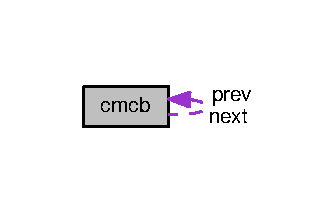
\includegraphics[width=161pt]{structcmcb__coll__graph}
\end{center}
\end{figure}
\subsection*{Data Fields}
\begin{DoxyCompactItemize}
\item 
int \hyperlink{structcmcb_ac765329451135abec74c45e1897abf26}{type}
\item 
void $\ast$ \hyperlink{structcmcb_a2f9031157d525501090fbadf7a1783cd}{beginning\+Addr}
\item 
int \hyperlink{structcmcb_a439227feff9d7f55384e8780cfc2eb82}{size}
\item 
int \hyperlink{structcmcb_af9658f4d1c59d6d251445c83931f0e55}{mem\+Size}
\item 
const char $\ast$ \hyperlink{structcmcb_a8f8f80d37794cde9472343e4487ba3eb}{name}
\item 
struct \hyperlink{structcmcb}{cmcb} $\ast$ \hyperlink{structcmcb_ae83456b67ed4fecca2703e070657e3c5}{next}
\item 
struct \hyperlink{structcmcb}{cmcb} $\ast$ \hyperlink{structcmcb_a6fd7de8eeff4983e21309c07178f6a77}{prev}
\end{DoxyCompactItemize}


\subsection{Field Documentation}
\index{cmcb@{cmcb}!beginning\+Addr@{beginning\+Addr}}
\index{beginning\+Addr@{beginning\+Addr}!cmcb@{cmcb}}
\subsubsection[{\texorpdfstring{beginning\+Addr}{beginningAddr}}]{\setlength{\rightskip}{0pt plus 5cm}void$\ast$ beginning\+Addr}\hypertarget{structcmcb_a2f9031157d525501090fbadf7a1783cd}{}\label{structcmcb_a2f9031157d525501090fbadf7a1783cd}
\index{cmcb@{cmcb}!mem\+Size@{mem\+Size}}
\index{mem\+Size@{mem\+Size}!cmcb@{cmcb}}
\subsubsection[{\texorpdfstring{mem\+Size}{memSize}}]{\setlength{\rightskip}{0pt plus 5cm}int mem\+Size}\hypertarget{structcmcb_af9658f4d1c59d6d251445c83931f0e55}{}\label{structcmcb_af9658f4d1c59d6d251445c83931f0e55}
\index{cmcb@{cmcb}!name@{name}}
\index{name@{name}!cmcb@{cmcb}}
\subsubsection[{\texorpdfstring{name}{name}}]{\setlength{\rightskip}{0pt plus 5cm}const char$\ast$ name}\hypertarget{structcmcb_a8f8f80d37794cde9472343e4487ba3eb}{}\label{structcmcb_a8f8f80d37794cde9472343e4487ba3eb}
\index{cmcb@{cmcb}!next@{next}}
\index{next@{next}!cmcb@{cmcb}}
\subsubsection[{\texorpdfstring{next}{next}}]{\setlength{\rightskip}{0pt plus 5cm}struct {\bf cmcb}$\ast$ next}\hypertarget{structcmcb_ae83456b67ed4fecca2703e070657e3c5}{}\label{structcmcb_ae83456b67ed4fecca2703e070657e3c5}
\index{cmcb@{cmcb}!prev@{prev}}
\index{prev@{prev}!cmcb@{cmcb}}
\subsubsection[{\texorpdfstring{prev}{prev}}]{\setlength{\rightskip}{0pt plus 5cm}struct {\bf cmcb}$\ast$ prev}\hypertarget{structcmcb_a6fd7de8eeff4983e21309c07178f6a77}{}\label{structcmcb_a6fd7de8eeff4983e21309c07178f6a77}
\index{cmcb@{cmcb}!size@{size}}
\index{size@{size}!cmcb@{cmcb}}
\subsubsection[{\texorpdfstring{size}{size}}]{\setlength{\rightskip}{0pt plus 5cm}int size}\hypertarget{structcmcb_a439227feff9d7f55384e8780cfc2eb82}{}\label{structcmcb_a439227feff9d7f55384e8780cfc2eb82}
\index{cmcb@{cmcb}!type@{type}}
\index{type@{type}!cmcb@{cmcb}}
\subsubsection[{\texorpdfstring{type}{type}}]{\setlength{\rightskip}{0pt plus 5cm}int type}\hypertarget{structcmcb_ac765329451135abec74c45e1897abf26}{}\label{structcmcb_ac765329451135abec74c45e1897abf26}


The documentation for this struct was generated from the following file\+:\begin{DoxyCompactItemize}
\item 
include/mem/\hyperlink{memory_control_8h}{memory\+Control.\+h}\end{DoxyCompactItemize}

\hypertarget{structcontext}{}\section{context Struct Reference}
\label{structcontext}\index{context@{context}}


{\ttfamily \#include $<$mpx\+\_\+supt.\+h$>$}

\subsection*{Data Fields}
\begin{DoxyCompactItemize}
\item 
\hyperlink{system_8h_a757de76cafbcddaac0d1632902fe4cb8}{u32int} \hyperlink{structcontext_abcc56997e8024ea8d5d3cf7e1ef6ae3a}{gs}
\item 
\hyperlink{system_8h_a757de76cafbcddaac0d1632902fe4cb8}{u32int} \hyperlink{structcontext_a59556586c5fc48990f50150d95a0735d}{fs}
\item 
\hyperlink{system_8h_a757de76cafbcddaac0d1632902fe4cb8}{u32int} \hyperlink{structcontext_aa9186bcc7f073d849fd12d4f2c649637}{es}
\item 
\hyperlink{system_8h_a757de76cafbcddaac0d1632902fe4cb8}{u32int} \hyperlink{structcontext_a27b615cc9d414c57f335c1744908fbd1}{ds}
\item 
\hyperlink{system_8h_a757de76cafbcddaac0d1632902fe4cb8}{u32int} \hyperlink{structcontext_ab42cc86f60a286d9cb20116b853239ff}{edi}
\item 
\hyperlink{system_8h_a757de76cafbcddaac0d1632902fe4cb8}{u32int} \hyperlink{structcontext_a031d176a324992b1ef7c3b7335383590}{esi}
\item 
\hyperlink{system_8h_a757de76cafbcddaac0d1632902fe4cb8}{u32int} \hyperlink{structcontext_a98b65807686fee47d4061d2f2ea8578a}{ebp}
\item 
\hyperlink{system_8h_a757de76cafbcddaac0d1632902fe4cb8}{u32int} \hyperlink{structcontext_a7c8cdb0e23278dc958565ee9a5ebb14b}{esp}
\item 
\hyperlink{system_8h_a757de76cafbcddaac0d1632902fe4cb8}{u32int} \hyperlink{structcontext_aab632bcfbdfeee937cc42940432af39a}{ebx}
\item 
\hyperlink{system_8h_a757de76cafbcddaac0d1632902fe4cb8}{u32int} \hyperlink{structcontext_aeef91c926bff500767180c01b413a537}{edx}
\item 
\hyperlink{system_8h_a757de76cafbcddaac0d1632902fe4cb8}{u32int} \hyperlink{structcontext_aab67c5aaaf6afb6a2c47a4c81fb0d567}{ecx}
\item 
\hyperlink{system_8h_a757de76cafbcddaac0d1632902fe4cb8}{u32int} \hyperlink{structcontext_aa4608f9844ee6e6e638c487a8c8aa14f}{eax}
\item 
\hyperlink{system_8h_a757de76cafbcddaac0d1632902fe4cb8}{u32int} \hyperlink{structcontext_ac6586230a521f5a60cded255700eaa79}{eip}
\item 
\hyperlink{system_8h_a757de76cafbcddaac0d1632902fe4cb8}{u32int} \hyperlink{structcontext_aff16eb39266599b77ad4025e1cf36c4e}{cs}
\item 
\hyperlink{system_8h_a757de76cafbcddaac0d1632902fe4cb8}{u32int} \hyperlink{structcontext_a1d2e9eee9e5db4c3658f2d72065463f3}{eflags}
\end{DoxyCompactItemize}


\subsection{Field Documentation}
\index{context@{context}!cs@{cs}}
\index{cs@{cs}!context@{context}}
\subsubsection[{\texorpdfstring{cs}{cs}}]{\setlength{\rightskip}{0pt plus 5cm}{\bf u32int} cs}\hypertarget{structcontext_aff16eb39266599b77ad4025e1cf36c4e}{}\label{structcontext_aff16eb39266599b77ad4025e1cf36c4e}
\index{context@{context}!ds@{ds}}
\index{ds@{ds}!context@{context}}
\subsubsection[{\texorpdfstring{ds}{ds}}]{\setlength{\rightskip}{0pt plus 5cm}{\bf u32int} ds}\hypertarget{structcontext_a27b615cc9d414c57f335c1744908fbd1}{}\label{structcontext_a27b615cc9d414c57f335c1744908fbd1}
\index{context@{context}!eax@{eax}}
\index{eax@{eax}!context@{context}}
\subsubsection[{\texorpdfstring{eax}{eax}}]{\setlength{\rightskip}{0pt plus 5cm}{\bf u32int} eax}\hypertarget{structcontext_aa4608f9844ee6e6e638c487a8c8aa14f}{}\label{structcontext_aa4608f9844ee6e6e638c487a8c8aa14f}
\index{context@{context}!ebp@{ebp}}
\index{ebp@{ebp}!context@{context}}
\subsubsection[{\texorpdfstring{ebp}{ebp}}]{\setlength{\rightskip}{0pt plus 5cm}{\bf u32int} ebp}\hypertarget{structcontext_a98b65807686fee47d4061d2f2ea8578a}{}\label{structcontext_a98b65807686fee47d4061d2f2ea8578a}
\index{context@{context}!ebx@{ebx}}
\index{ebx@{ebx}!context@{context}}
\subsubsection[{\texorpdfstring{ebx}{ebx}}]{\setlength{\rightskip}{0pt plus 5cm}{\bf u32int} ebx}\hypertarget{structcontext_aab632bcfbdfeee937cc42940432af39a}{}\label{structcontext_aab632bcfbdfeee937cc42940432af39a}
\index{context@{context}!ecx@{ecx}}
\index{ecx@{ecx}!context@{context}}
\subsubsection[{\texorpdfstring{ecx}{ecx}}]{\setlength{\rightskip}{0pt plus 5cm}{\bf u32int} ecx}\hypertarget{structcontext_aab67c5aaaf6afb6a2c47a4c81fb0d567}{}\label{structcontext_aab67c5aaaf6afb6a2c47a4c81fb0d567}
\index{context@{context}!edi@{edi}}
\index{edi@{edi}!context@{context}}
\subsubsection[{\texorpdfstring{edi}{edi}}]{\setlength{\rightskip}{0pt plus 5cm}{\bf u32int} edi}\hypertarget{structcontext_ab42cc86f60a286d9cb20116b853239ff}{}\label{structcontext_ab42cc86f60a286d9cb20116b853239ff}
\index{context@{context}!edx@{edx}}
\index{edx@{edx}!context@{context}}
\subsubsection[{\texorpdfstring{edx}{edx}}]{\setlength{\rightskip}{0pt plus 5cm}{\bf u32int} edx}\hypertarget{structcontext_aeef91c926bff500767180c01b413a537}{}\label{structcontext_aeef91c926bff500767180c01b413a537}
\index{context@{context}!eflags@{eflags}}
\index{eflags@{eflags}!context@{context}}
\subsubsection[{\texorpdfstring{eflags}{eflags}}]{\setlength{\rightskip}{0pt plus 5cm}{\bf u32int} eflags}\hypertarget{structcontext_a1d2e9eee9e5db4c3658f2d72065463f3}{}\label{structcontext_a1d2e9eee9e5db4c3658f2d72065463f3}
\index{context@{context}!eip@{eip}}
\index{eip@{eip}!context@{context}}
\subsubsection[{\texorpdfstring{eip}{eip}}]{\setlength{\rightskip}{0pt plus 5cm}{\bf u32int} eip}\hypertarget{structcontext_ac6586230a521f5a60cded255700eaa79}{}\label{structcontext_ac6586230a521f5a60cded255700eaa79}
\index{context@{context}!es@{es}}
\index{es@{es}!context@{context}}
\subsubsection[{\texorpdfstring{es}{es}}]{\setlength{\rightskip}{0pt plus 5cm}{\bf u32int} es}\hypertarget{structcontext_aa9186bcc7f073d849fd12d4f2c649637}{}\label{structcontext_aa9186bcc7f073d849fd12d4f2c649637}
\index{context@{context}!esi@{esi}}
\index{esi@{esi}!context@{context}}
\subsubsection[{\texorpdfstring{esi}{esi}}]{\setlength{\rightskip}{0pt plus 5cm}{\bf u32int} esi}\hypertarget{structcontext_a031d176a324992b1ef7c3b7335383590}{}\label{structcontext_a031d176a324992b1ef7c3b7335383590}
\index{context@{context}!esp@{esp}}
\index{esp@{esp}!context@{context}}
\subsubsection[{\texorpdfstring{esp}{esp}}]{\setlength{\rightskip}{0pt plus 5cm}{\bf u32int} esp}\hypertarget{structcontext_a7c8cdb0e23278dc958565ee9a5ebb14b}{}\label{structcontext_a7c8cdb0e23278dc958565ee9a5ebb14b}
\index{context@{context}!fs@{fs}}
\index{fs@{fs}!context@{context}}
\subsubsection[{\texorpdfstring{fs}{fs}}]{\setlength{\rightskip}{0pt plus 5cm}{\bf u32int} fs}\hypertarget{structcontext_a59556586c5fc48990f50150d95a0735d}{}\label{structcontext_a59556586c5fc48990f50150d95a0735d}
\index{context@{context}!gs@{gs}}
\index{gs@{gs}!context@{context}}
\subsubsection[{\texorpdfstring{gs}{gs}}]{\setlength{\rightskip}{0pt plus 5cm}{\bf u32int} gs}\hypertarget{structcontext_abcc56997e8024ea8d5d3cf7e1ef6ae3a}{}\label{structcontext_abcc56997e8024ea8d5d3cf7e1ef6ae3a}


The documentation for this struct was generated from the following file\+:\begin{DoxyCompactItemize}
\item 
include/modules/\hyperlink{mpx__supt_8h}{mpx\+\_\+supt.\+h}\end{DoxyCompactItemize}

\hypertarget{structdate__time}{}\section{date\+\_\+time Struct Reference}
\label{structdate__time}\index{date\+\_\+time@{date\+\_\+time}}


{\ttfamily \#include $<$time.\+h$>$}

\subsection*{Data Fields}
\begin{DoxyCompactItemize}
\item 
int \hyperlink{structdate__time_a90c2ace84e5523d06b7162ea5928acc1}{sec}
\item 
int \hyperlink{structdate__time_a3e202b201e6255d975cd6d3aff1f5a4d}{min}
\item 
int \hyperlink{structdate__time_a15df9ba285cfd842f284025f904edc9c}{hour}
\item 
int \hyperlink{structdate__time_a65f1a8d2d8998298122653d29b282039}{day\+\_\+w}
\item 
int \hyperlink{structdate__time_a02c5941dc0947f075ee0d8f3362921bf}{day\+\_\+m}
\item 
int \hyperlink{structdate__time_ae32b944876e247e9a9fae3371d54c71f}{day\+\_\+y}
\item 
int \hyperlink{structdate__time_a25b602fa15f03b01f61a900f1f68a67d}{mon}
\item 
int \hyperlink{structdate__time_abeac221e38b7b9ce7df8722c842bf671}{year}
\end{DoxyCompactItemize}


\subsection{Detailed Description}
Structure representing a date and time. 

\subsection{Field Documentation}
\index{date\+\_\+time@{date\+\_\+time}!day\+\_\+m@{day\+\_\+m}}
\index{day\+\_\+m@{day\+\_\+m}!date\+\_\+time@{date\+\_\+time}}
\subsubsection[{\texorpdfstring{day\+\_\+m}{day_m}}]{\setlength{\rightskip}{0pt plus 5cm}int day\+\_\+m}\hypertarget{structdate__time_a02c5941dc0947f075ee0d8f3362921bf}{}\label{structdate__time_a02c5941dc0947f075ee0d8f3362921bf}
\index{date\+\_\+time@{date\+\_\+time}!day\+\_\+w@{day\+\_\+w}}
\index{day\+\_\+w@{day\+\_\+w}!date\+\_\+time@{date\+\_\+time}}
\subsubsection[{\texorpdfstring{day\+\_\+w}{day_w}}]{\setlength{\rightskip}{0pt plus 5cm}int day\+\_\+w}\hypertarget{structdate__time_a65f1a8d2d8998298122653d29b282039}{}\label{structdate__time_a65f1a8d2d8998298122653d29b282039}
\index{date\+\_\+time@{date\+\_\+time}!day\+\_\+y@{day\+\_\+y}}
\index{day\+\_\+y@{day\+\_\+y}!date\+\_\+time@{date\+\_\+time}}
\subsubsection[{\texorpdfstring{day\+\_\+y}{day_y}}]{\setlength{\rightskip}{0pt plus 5cm}int day\+\_\+y}\hypertarget{structdate__time_ae32b944876e247e9a9fae3371d54c71f}{}\label{structdate__time_ae32b944876e247e9a9fae3371d54c71f}
\index{date\+\_\+time@{date\+\_\+time}!hour@{hour}}
\index{hour@{hour}!date\+\_\+time@{date\+\_\+time}}
\subsubsection[{\texorpdfstring{hour}{hour}}]{\setlength{\rightskip}{0pt plus 5cm}int hour}\hypertarget{structdate__time_a15df9ba285cfd842f284025f904edc9c}{}\label{structdate__time_a15df9ba285cfd842f284025f904edc9c}
\index{date\+\_\+time@{date\+\_\+time}!min@{min}}
\index{min@{min}!date\+\_\+time@{date\+\_\+time}}
\subsubsection[{\texorpdfstring{min}{min}}]{\setlength{\rightskip}{0pt plus 5cm}int min}\hypertarget{structdate__time_a3e202b201e6255d975cd6d3aff1f5a4d}{}\label{structdate__time_a3e202b201e6255d975cd6d3aff1f5a4d}
\index{date\+\_\+time@{date\+\_\+time}!mon@{mon}}
\index{mon@{mon}!date\+\_\+time@{date\+\_\+time}}
\subsubsection[{\texorpdfstring{mon}{mon}}]{\setlength{\rightskip}{0pt plus 5cm}int mon}\hypertarget{structdate__time_a25b602fa15f03b01f61a900f1f68a67d}{}\label{structdate__time_a25b602fa15f03b01f61a900f1f68a67d}
\index{date\+\_\+time@{date\+\_\+time}!sec@{sec}}
\index{sec@{sec}!date\+\_\+time@{date\+\_\+time}}
\subsubsection[{\texorpdfstring{sec}{sec}}]{\setlength{\rightskip}{0pt plus 5cm}int sec}\hypertarget{structdate__time_a90c2ace84e5523d06b7162ea5928acc1}{}\label{structdate__time_a90c2ace84e5523d06b7162ea5928acc1}
\index{date\+\_\+time@{date\+\_\+time}!year@{year}}
\index{year@{year}!date\+\_\+time@{date\+\_\+time}}
\subsubsection[{\texorpdfstring{year}{year}}]{\setlength{\rightskip}{0pt plus 5cm}int year}\hypertarget{structdate__time_abeac221e38b7b9ce7df8722c842bf671}{}\label{structdate__time_abeac221e38b7b9ce7df8722c842bf671}


The documentation for this struct was generated from the following file\+:\begin{DoxyCompactItemize}
\item 
include/\hyperlink{time_8h}{time.\+h}\end{DoxyCompactItemize}

\hypertarget{structdir__entry}{}\section{dir\+\_\+entry Struct Reference}
\label{structdir__entry}\index{dir\+\_\+entry@{dir\+\_\+entry}}


{\ttfamily \#include $<$fat.\+h$>$}

\subsection*{Data Fields}
\begin{DoxyCompactItemize}
\item 
unsigned char \hyperlink{structdir__entry_aa45f4647093034458ab8972553e58829}{filename} \mbox{[}9\mbox{]}
\item 
unsigned char \hyperlink{structdir__entry_aa7a3c21c76cf5259f07096aa3cb7be7b}{extension} \mbox{[}4\mbox{]}
\item 
uint8\+\_\+t \hyperlink{structdir__entry_a983149395439fbc9ca8497076b75fd6b}{attributes}
\item 
uint16\+\_\+t \hyperlink{structdir__entry_a5a6ed8c04a3db86066924b1a1bf4dad3}{reserved}
\item 
uint16\+\_\+t \hyperlink{structdir__entry_a2b2b18a3fb988470278b1217abe946ab}{creation\+Time}
\item 
uint16\+\_\+t \hyperlink{structdir__entry_ab00be6268bf4c4f4b6014f056e27ba45}{creation\+Date}
\item 
uint16\+\_\+t \hyperlink{structdir__entry_a242e5c055f30cde4b8c0e121fe25deab}{last\+Access}
\item 
uint16\+\_\+t \hyperlink{structdir__entry_a56a1f4f280fba6da7541dbe629342781}{ignore}
\item 
uint16\+\_\+t \hyperlink{structdir__entry_ab140bb773b2ff0ddf7199efc083ce037}{last\+Write\+Time}
\item 
uint16\+\_\+t \hyperlink{structdir__entry_a26f462d6e4410d502149973ee6c216fd}{last\+Write\+Date}
\item 
uint16\+\_\+t \hyperlink{structdir__entry_a1b249a3e9b17eda2684039fc366f6131}{first\+Logical\+Cluster}
\item 
uint32\+\_\+t \hyperlink{structdir__entry_a48f46ad02b77a00b795d15626ba1d42e}{file\+Size}
\end{DoxyCompactItemize}


\subsection{Detailed Description}
Struct representing a directory entry 

\subsection{Field Documentation}
\index{dir\+\_\+entry@{dir\+\_\+entry}!attributes@{attributes}}
\index{attributes@{attributes}!dir\+\_\+entry@{dir\+\_\+entry}}
\subsubsection[{\texorpdfstring{attributes}{attributes}}]{\setlength{\rightskip}{0pt plus 5cm}uint8\+\_\+t attributes}\hypertarget{structdir__entry_a983149395439fbc9ca8497076b75fd6b}{}\label{structdir__entry_a983149395439fbc9ca8497076b75fd6b}
\index{dir\+\_\+entry@{dir\+\_\+entry}!creation\+Date@{creation\+Date}}
\index{creation\+Date@{creation\+Date}!dir\+\_\+entry@{dir\+\_\+entry}}
\subsubsection[{\texorpdfstring{creation\+Date}{creationDate}}]{\setlength{\rightskip}{0pt plus 5cm}uint16\+\_\+t creation\+Date}\hypertarget{structdir__entry_ab00be6268bf4c4f4b6014f056e27ba45}{}\label{structdir__entry_ab00be6268bf4c4f4b6014f056e27ba45}
\index{dir\+\_\+entry@{dir\+\_\+entry}!creation\+Time@{creation\+Time}}
\index{creation\+Time@{creation\+Time}!dir\+\_\+entry@{dir\+\_\+entry}}
\subsubsection[{\texorpdfstring{creation\+Time}{creationTime}}]{\setlength{\rightskip}{0pt plus 5cm}uint16\+\_\+t creation\+Time}\hypertarget{structdir__entry_a2b2b18a3fb988470278b1217abe946ab}{}\label{structdir__entry_a2b2b18a3fb988470278b1217abe946ab}
\index{dir\+\_\+entry@{dir\+\_\+entry}!extension@{extension}}
\index{extension@{extension}!dir\+\_\+entry@{dir\+\_\+entry}}
\subsubsection[{\texorpdfstring{extension}{extension}}]{\setlength{\rightskip}{0pt plus 5cm}unsigned char extension\mbox{[}4\mbox{]}}\hypertarget{structdir__entry_aa7a3c21c76cf5259f07096aa3cb7be7b}{}\label{structdir__entry_aa7a3c21c76cf5259f07096aa3cb7be7b}
\index{dir\+\_\+entry@{dir\+\_\+entry}!filename@{filename}}
\index{filename@{filename}!dir\+\_\+entry@{dir\+\_\+entry}}
\subsubsection[{\texorpdfstring{filename}{filename}}]{\setlength{\rightskip}{0pt plus 5cm}unsigned char filename\mbox{[}9\mbox{]}}\hypertarget{structdir__entry_aa45f4647093034458ab8972553e58829}{}\label{structdir__entry_aa45f4647093034458ab8972553e58829}
\index{dir\+\_\+entry@{dir\+\_\+entry}!file\+Size@{file\+Size}}
\index{file\+Size@{file\+Size}!dir\+\_\+entry@{dir\+\_\+entry}}
\subsubsection[{\texorpdfstring{file\+Size}{fileSize}}]{\setlength{\rightskip}{0pt plus 5cm}uint32\+\_\+t file\+Size}\hypertarget{structdir__entry_a48f46ad02b77a00b795d15626ba1d42e}{}\label{structdir__entry_a48f46ad02b77a00b795d15626ba1d42e}
\index{dir\+\_\+entry@{dir\+\_\+entry}!first\+Logical\+Cluster@{first\+Logical\+Cluster}}
\index{first\+Logical\+Cluster@{first\+Logical\+Cluster}!dir\+\_\+entry@{dir\+\_\+entry}}
\subsubsection[{\texorpdfstring{first\+Logical\+Cluster}{firstLogicalCluster}}]{\setlength{\rightskip}{0pt plus 5cm}uint16\+\_\+t first\+Logical\+Cluster}\hypertarget{structdir__entry_a1b249a3e9b17eda2684039fc366f6131}{}\label{structdir__entry_a1b249a3e9b17eda2684039fc366f6131}
\index{dir\+\_\+entry@{dir\+\_\+entry}!ignore@{ignore}}
\index{ignore@{ignore}!dir\+\_\+entry@{dir\+\_\+entry}}
\subsubsection[{\texorpdfstring{ignore}{ignore}}]{\setlength{\rightskip}{0pt plus 5cm}uint16\+\_\+t ignore}\hypertarget{structdir__entry_a56a1f4f280fba6da7541dbe629342781}{}\label{structdir__entry_a56a1f4f280fba6da7541dbe629342781}
\index{dir\+\_\+entry@{dir\+\_\+entry}!last\+Access@{last\+Access}}
\index{last\+Access@{last\+Access}!dir\+\_\+entry@{dir\+\_\+entry}}
\subsubsection[{\texorpdfstring{last\+Access}{lastAccess}}]{\setlength{\rightskip}{0pt plus 5cm}uint16\+\_\+t last\+Access}\hypertarget{structdir__entry_a242e5c055f30cde4b8c0e121fe25deab}{}\label{structdir__entry_a242e5c055f30cde4b8c0e121fe25deab}
\index{dir\+\_\+entry@{dir\+\_\+entry}!last\+Write\+Date@{last\+Write\+Date}}
\index{last\+Write\+Date@{last\+Write\+Date}!dir\+\_\+entry@{dir\+\_\+entry}}
\subsubsection[{\texorpdfstring{last\+Write\+Date}{lastWriteDate}}]{\setlength{\rightskip}{0pt plus 5cm}uint16\+\_\+t last\+Write\+Date}\hypertarget{structdir__entry_a26f462d6e4410d502149973ee6c216fd}{}\label{structdir__entry_a26f462d6e4410d502149973ee6c216fd}
\index{dir\+\_\+entry@{dir\+\_\+entry}!last\+Write\+Time@{last\+Write\+Time}}
\index{last\+Write\+Time@{last\+Write\+Time}!dir\+\_\+entry@{dir\+\_\+entry}}
\subsubsection[{\texorpdfstring{last\+Write\+Time}{lastWriteTime}}]{\setlength{\rightskip}{0pt plus 5cm}uint16\+\_\+t last\+Write\+Time}\hypertarget{structdir__entry_ab140bb773b2ff0ddf7199efc083ce037}{}\label{structdir__entry_ab140bb773b2ff0ddf7199efc083ce037}
\index{dir\+\_\+entry@{dir\+\_\+entry}!reserved@{reserved}}
\index{reserved@{reserved}!dir\+\_\+entry@{dir\+\_\+entry}}
\subsubsection[{\texorpdfstring{reserved}{reserved}}]{\setlength{\rightskip}{0pt plus 5cm}uint16\+\_\+t reserved}\hypertarget{structdir__entry_a5a6ed8c04a3db86066924b1a1bf4dad3}{}\label{structdir__entry_a5a6ed8c04a3db86066924b1a1bf4dad3}


The documentation for this struct was generated from the following file\+:\begin{DoxyCompactItemize}
\item 
r6/\hyperlink{fat_8h}{fat.\+h}\end{DoxyCompactItemize}

\hypertarget{structfat__tables}{}\section{fat\+\_\+tables Struct Reference}
\label{structfat__tables}\index{fat\+\_\+tables@{fat\+\_\+tables}}


{\ttfamily \#include $<$fat.\+h$>$}

\subsection*{Data Fields}
\begin{DoxyCompactItemize}
\item 
int \hyperlink{structfat__tables_a75b15f0e26b4ccf3195772b134b660ec}{num\+Entries}
\item 
uint16\+\_\+t $\ast$ \hyperlink{structfat__tables_a45f86c4c2f51c8fe61e736c8d9449abf}{fat1}
\item 
uint16\+\_\+t $\ast$ \hyperlink{structfat__tables_a639b4d55f6ba2085dc48551d4234af67}{fat2}
\end{DoxyCompactItemize}


\subsection{Detailed Description}
Struct containing the F\+AT table information 

\subsection{Field Documentation}
\index{fat\+\_\+tables@{fat\+\_\+tables}!fat1@{fat1}}
\index{fat1@{fat1}!fat\+\_\+tables@{fat\+\_\+tables}}
\subsubsection[{\texorpdfstring{fat1}{fat1}}]{\setlength{\rightskip}{0pt plus 5cm}uint16\+\_\+t$\ast$ fat1}\hypertarget{structfat__tables_a45f86c4c2f51c8fe61e736c8d9449abf}{}\label{structfat__tables_a45f86c4c2f51c8fe61e736c8d9449abf}
\index{fat\+\_\+tables@{fat\+\_\+tables}!fat2@{fat2}}
\index{fat2@{fat2}!fat\+\_\+tables@{fat\+\_\+tables}}
\subsubsection[{\texorpdfstring{fat2}{fat2}}]{\setlength{\rightskip}{0pt plus 5cm}uint16\+\_\+t$\ast$ fat2}\hypertarget{structfat__tables_a639b4d55f6ba2085dc48551d4234af67}{}\label{structfat__tables_a639b4d55f6ba2085dc48551d4234af67}
\index{fat\+\_\+tables@{fat\+\_\+tables}!num\+Entries@{num\+Entries}}
\index{num\+Entries@{num\+Entries}!fat\+\_\+tables@{fat\+\_\+tables}}
\subsubsection[{\texorpdfstring{num\+Entries}{numEntries}}]{\setlength{\rightskip}{0pt plus 5cm}int num\+Entries}\hypertarget{structfat__tables_a75b15f0e26b4ccf3195772b134b660ec}{}\label{structfat__tables_a75b15f0e26b4ccf3195772b134b660ec}


The documentation for this struct was generated from the following file\+:\begin{DoxyCompactItemize}
\item 
r6/\hyperlink{fat_8h}{fat.\+h}\end{DoxyCompactItemize}

\hypertarget{structfooter}{}\section{footer Struct Reference}
\label{structfooter}\index{footer@{footer}}


{\ttfamily \#include $<$heap.\+h$>$}



Collaboration diagram for footer\+:\nopagebreak
\begin{figure}[H]
\begin{center}
\leavevmode
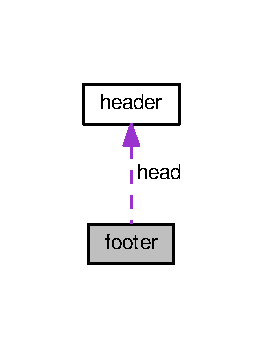
\includegraphics[width=128pt]{structfooter__coll__graph}
\end{center}
\end{figure}
\subsection*{Data Fields}
\begin{DoxyCompactItemize}
\item 
\hyperlink{structheader}{header} \hyperlink{structfooter_a0e77a30e5469bc62f17579602fc74bc3}{head}
\end{DoxyCompactItemize}


\subsection{Detailed Description}
Heap allocation footer. 

\subsection{Field Documentation}
\index{footer@{footer}!head@{head}}
\index{head@{head}!footer@{footer}}
\subsubsection[{\texorpdfstring{head}{head}}]{\setlength{\rightskip}{0pt plus 5cm}{\bf header} head}\hypertarget{structfooter_a0e77a30e5469bc62f17579602fc74bc3}{}\label{structfooter_a0e77a30e5469bc62f17579602fc74bc3}


The documentation for this struct was generated from the following file\+:\begin{DoxyCompactItemize}
\item 
include/mem/\hyperlink{heap_8h}{heap.\+h}\end{DoxyCompactItemize}

\hypertarget{structfunction_def}{}\section{function\+Def Struct Reference}
\label{structfunction_def}\index{function\+Def@{function\+Def}}


{\ttfamily \#include $<$com\+Handler.\+h$>$}

\subsection*{Data Fields}
\begin{DoxyCompactItemize}
\item 
char $\ast$ \hyperlink{structfunction_def_a5ac083a645d964373f022d03df4849c8}{name}
\item 
const char $\ast$ \hyperlink{structfunction_def_ab4c259a269a580945600ed07ecaebffa}{help\+String}
\item 
const char $\ast$($\ast$ \hyperlink{structfunction_def_a00d6d4cc8307840fbc601f6fa55dafa3}{func\+Pointer} )(char $\ast$$\ast$args, int num\+Args)
\end{DoxyCompactItemize}


\subsection{Field Documentation}
\index{function\+Def@{function\+Def}!func\+Pointer@{func\+Pointer}}
\index{func\+Pointer@{func\+Pointer}!function\+Def@{function\+Def}}
\subsubsection[{\texorpdfstring{func\+Pointer}{funcPointer}}]{\setlength{\rightskip}{0pt plus 5cm}const char$\ast$($\ast$ func\+Pointer) (char $\ast$$\ast$args, int num\+Args)}\hypertarget{structfunction_def_a00d6d4cc8307840fbc601f6fa55dafa3}{}\label{structfunction_def_a00d6d4cc8307840fbc601f6fa55dafa3}
\index{function\+Def@{function\+Def}!help\+String@{help\+String}}
\index{help\+String@{help\+String}!function\+Def@{function\+Def}}
\subsubsection[{\texorpdfstring{help\+String}{helpString}}]{\setlength{\rightskip}{0pt plus 5cm}const char$\ast$ help\+String}\hypertarget{structfunction_def_ab4c259a269a580945600ed07ecaebffa}{}\label{structfunction_def_ab4c259a269a580945600ed07ecaebffa}
\index{function\+Def@{function\+Def}!name@{name}}
\index{name@{name}!function\+Def@{function\+Def}}
\subsubsection[{\texorpdfstring{name}{name}}]{\setlength{\rightskip}{0pt plus 5cm}char$\ast$ name}\hypertarget{structfunction_def_a5ac083a645d964373f022d03df4849c8}{}\label{structfunction_def_a5ac083a645d964373f022d03df4849c8}


The documentation for this struct was generated from the following file\+:\begin{DoxyCompactItemize}
\item 
include/core/\hyperlink{com_handler_8h}{com\+Handler.\+h}\end{DoxyCompactItemize}

\hypertarget{structgdt__descriptor__struct}{}\section{gdt\+\_\+descriptor\+\_\+struct Struct Reference}
\label{structgdt__descriptor__struct}\index{gdt\+\_\+descriptor\+\_\+struct@{gdt\+\_\+descriptor\+\_\+struct}}


{\ttfamily \#include $<$tables.\+h$>$}

\subsection*{Data Fields}
\begin{DoxyCompactItemize}
\item 
\hyperlink{system_8h_a863d9497073aad2b991aeab2211d87af}{u16int} \hyperlink{structgdt__descriptor__struct_a68fd3b4f6c14a331ca9b226cbf122e13}{limit}
\item 
\hyperlink{system_8h_a757de76cafbcddaac0d1632902fe4cb8}{u32int} \hyperlink{structgdt__descriptor__struct_ab5763c2b18c825c8b8fba44b2e60ddc1}{base}
\end{DoxyCompactItemize}


\subsection{Field Documentation}
\index{gdt\+\_\+descriptor\+\_\+struct@{gdt\+\_\+descriptor\+\_\+struct}!base@{base}}
\index{base@{base}!gdt\+\_\+descriptor\+\_\+struct@{gdt\+\_\+descriptor\+\_\+struct}}
\subsubsection[{\texorpdfstring{base}{base}}]{\setlength{\rightskip}{0pt plus 5cm}{\bf u32int} base}\hypertarget{structgdt__descriptor__struct_ab5763c2b18c825c8b8fba44b2e60ddc1}{}\label{structgdt__descriptor__struct_ab5763c2b18c825c8b8fba44b2e60ddc1}
\index{gdt\+\_\+descriptor\+\_\+struct@{gdt\+\_\+descriptor\+\_\+struct}!limit@{limit}}
\index{limit@{limit}!gdt\+\_\+descriptor\+\_\+struct@{gdt\+\_\+descriptor\+\_\+struct}}
\subsubsection[{\texorpdfstring{limit}{limit}}]{\setlength{\rightskip}{0pt plus 5cm}{\bf u16int} limit}\hypertarget{structgdt__descriptor__struct_a68fd3b4f6c14a331ca9b226cbf122e13}{}\label{structgdt__descriptor__struct_a68fd3b4f6c14a331ca9b226cbf122e13}


The documentation for this struct was generated from the following file\+:\begin{DoxyCompactItemize}
\item 
include/core/\hyperlink{tables_8h}{tables.\+h}\end{DoxyCompactItemize}

\hypertarget{structgdt__entry__struct}{}\section{gdt\+\_\+entry\+\_\+struct Struct Reference}
\label{structgdt__entry__struct}\index{gdt\+\_\+entry\+\_\+struct@{gdt\+\_\+entry\+\_\+struct}}


{\ttfamily \#include $<$tables.\+h$>$}

\subsection*{Data Fields}
\begin{DoxyCompactItemize}
\item 
\hyperlink{system_8h_a863d9497073aad2b991aeab2211d87af}{u16int} \hyperlink{structgdt__entry__struct_af9013229edfb91d4820f66b8df890ce3}{limit\+\_\+low}
\item 
\hyperlink{system_8h_a863d9497073aad2b991aeab2211d87af}{u16int} \hyperlink{structgdt__entry__struct_a0a776dced2c26f16298425cde39f8364}{base\+\_\+low}
\item 
\hyperlink{system_8h_a1026e682ffdadc1701c42cd44ce9efcf}{u8int} \hyperlink{structgdt__entry__struct_a35c709a004babd09046db9f667ba0646}{base\+\_\+mid}
\item 
\hyperlink{system_8h_a1026e682ffdadc1701c42cd44ce9efcf}{u8int} \hyperlink{structgdt__entry__struct_a360a726ac0b61d9e4e1be3ad34f80244}{access}
\item 
\hyperlink{system_8h_a1026e682ffdadc1701c42cd44ce9efcf}{u8int} \hyperlink{structgdt__entry__struct_a138dda98fcd4738346af61bcca8cf4b4}{flags}
\item 
\hyperlink{system_8h_a1026e682ffdadc1701c42cd44ce9efcf}{u8int} \hyperlink{structgdt__entry__struct_a706c81b840522a69ab6e6e941630d5e4}{base\+\_\+high}
\end{DoxyCompactItemize}


\subsection{Field Documentation}
\index{gdt\+\_\+entry\+\_\+struct@{gdt\+\_\+entry\+\_\+struct}!access@{access}}
\index{access@{access}!gdt\+\_\+entry\+\_\+struct@{gdt\+\_\+entry\+\_\+struct}}
\subsubsection[{\texorpdfstring{access}{access}}]{\setlength{\rightskip}{0pt plus 5cm}{\bf u8int} access}\hypertarget{structgdt__entry__struct_a360a726ac0b61d9e4e1be3ad34f80244}{}\label{structgdt__entry__struct_a360a726ac0b61d9e4e1be3ad34f80244}
\index{gdt\+\_\+entry\+\_\+struct@{gdt\+\_\+entry\+\_\+struct}!base\+\_\+high@{base\+\_\+high}}
\index{base\+\_\+high@{base\+\_\+high}!gdt\+\_\+entry\+\_\+struct@{gdt\+\_\+entry\+\_\+struct}}
\subsubsection[{\texorpdfstring{base\+\_\+high}{base_high}}]{\setlength{\rightskip}{0pt plus 5cm}{\bf u8int} base\+\_\+high}\hypertarget{structgdt__entry__struct_a706c81b840522a69ab6e6e941630d5e4}{}\label{structgdt__entry__struct_a706c81b840522a69ab6e6e941630d5e4}
\index{gdt\+\_\+entry\+\_\+struct@{gdt\+\_\+entry\+\_\+struct}!base\+\_\+low@{base\+\_\+low}}
\index{base\+\_\+low@{base\+\_\+low}!gdt\+\_\+entry\+\_\+struct@{gdt\+\_\+entry\+\_\+struct}}
\subsubsection[{\texorpdfstring{base\+\_\+low}{base_low}}]{\setlength{\rightskip}{0pt plus 5cm}{\bf u16int} base\+\_\+low}\hypertarget{structgdt__entry__struct_a0a776dced2c26f16298425cde39f8364}{}\label{structgdt__entry__struct_a0a776dced2c26f16298425cde39f8364}
\index{gdt\+\_\+entry\+\_\+struct@{gdt\+\_\+entry\+\_\+struct}!base\+\_\+mid@{base\+\_\+mid}}
\index{base\+\_\+mid@{base\+\_\+mid}!gdt\+\_\+entry\+\_\+struct@{gdt\+\_\+entry\+\_\+struct}}
\subsubsection[{\texorpdfstring{base\+\_\+mid}{base_mid}}]{\setlength{\rightskip}{0pt plus 5cm}{\bf u8int} base\+\_\+mid}\hypertarget{structgdt__entry__struct_a35c709a004babd09046db9f667ba0646}{}\label{structgdt__entry__struct_a35c709a004babd09046db9f667ba0646}
\index{gdt\+\_\+entry\+\_\+struct@{gdt\+\_\+entry\+\_\+struct}!flags@{flags}}
\index{flags@{flags}!gdt\+\_\+entry\+\_\+struct@{gdt\+\_\+entry\+\_\+struct}}
\subsubsection[{\texorpdfstring{flags}{flags}}]{\setlength{\rightskip}{0pt plus 5cm}{\bf u8int} flags}\hypertarget{structgdt__entry__struct_a138dda98fcd4738346af61bcca8cf4b4}{}\label{structgdt__entry__struct_a138dda98fcd4738346af61bcca8cf4b4}
\index{gdt\+\_\+entry\+\_\+struct@{gdt\+\_\+entry\+\_\+struct}!limit\+\_\+low@{limit\+\_\+low}}
\index{limit\+\_\+low@{limit\+\_\+low}!gdt\+\_\+entry\+\_\+struct@{gdt\+\_\+entry\+\_\+struct}}
\subsubsection[{\texorpdfstring{limit\+\_\+low}{limit_low}}]{\setlength{\rightskip}{0pt plus 5cm}{\bf u16int} limit\+\_\+low}\hypertarget{structgdt__entry__struct_af9013229edfb91d4820f66b8df890ce3}{}\label{structgdt__entry__struct_af9013229edfb91d4820f66b8df890ce3}


The documentation for this struct was generated from the following file\+:\begin{DoxyCompactItemize}
\item 
include/core/\hyperlink{tables_8h}{tables.\+h}\end{DoxyCompactItemize}

\hypertarget{structheader}{}\section{header Struct Reference}
\label{structheader}\index{header@{header}}


{\ttfamily \#include $<$heap.\+h$>$}

\subsection*{Data Fields}
\begin{DoxyCompactItemize}
\item 
int \hyperlink{structheader_a439227feff9d7f55384e8780cfc2eb82}{size}
\item 
int \hyperlink{structheader_af535dc35cc74e67b62de5a0a3540becd}{index\+\_\+id}
\end{DoxyCompactItemize}


\subsection{Detailed Description}
Heap allocation header. 

\subsection{Field Documentation}
\index{header@{header}!index\+\_\+id@{index\+\_\+id}}
\index{index\+\_\+id@{index\+\_\+id}!header@{header}}
\subsubsection[{\texorpdfstring{index\+\_\+id}{index_id}}]{\setlength{\rightskip}{0pt plus 5cm}int index\+\_\+id}\hypertarget{structheader_af535dc35cc74e67b62de5a0a3540becd}{}\label{structheader_af535dc35cc74e67b62de5a0a3540becd}
\index{header@{header}!size@{size}}
\index{size@{size}!header@{header}}
\subsubsection[{\texorpdfstring{size}{size}}]{\setlength{\rightskip}{0pt plus 5cm}int size}\hypertarget{structheader_a439227feff9d7f55384e8780cfc2eb82}{}\label{structheader_a439227feff9d7f55384e8780cfc2eb82}


The documentation for this struct was generated from the following file\+:\begin{DoxyCompactItemize}
\item 
include/mem/\hyperlink{heap_8h}{heap.\+h}\end{DoxyCompactItemize}

\hypertarget{structheap}{}\section{heap Struct Reference}
\label{structheap}\index{heap@{heap}}


{\ttfamily \#include $<$heap.\+h$>$}



Collaboration diagram for heap\+:\nopagebreak
\begin{figure}[H]
\begin{center}
\leavevmode
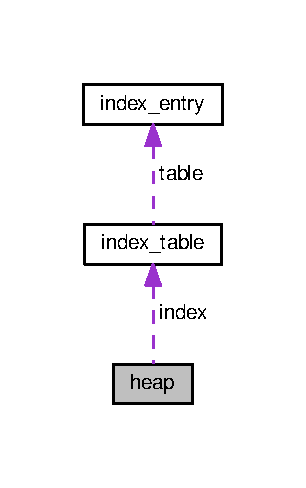
\includegraphics[width=147pt]{structheap__coll__graph}
\end{center}
\end{figure}
\subsection*{Data Fields}
\begin{DoxyCompactItemize}
\item 
\hyperlink{structindex__table}{index\+\_\+table} \hyperlink{structheap_af44ecb378e6839e4c91808d259825274}{index}
\item 
\hyperlink{system_8h_a757de76cafbcddaac0d1632902fe4cb8}{u32int} \hyperlink{structheap_ab5763c2b18c825c8b8fba44b2e60ddc1}{base}
\item 
\hyperlink{system_8h_a757de76cafbcddaac0d1632902fe4cb8}{u32int} \hyperlink{structheap_aff98f60fdff673e586a88d147da4798c}{max\+\_\+size}
\item 
\hyperlink{system_8h_a757de76cafbcddaac0d1632902fe4cb8}{u32int} \hyperlink{structheap_af515ec763221e45adce632886c4cb888}{min\+\_\+size}
\end{DoxyCompactItemize}


\subsection{Detailed Description}
Heap structure 

\subsection{Field Documentation}
\index{heap@{heap}!base@{base}}
\index{base@{base}!heap@{heap}}
\subsubsection[{\texorpdfstring{base}{base}}]{\setlength{\rightskip}{0pt plus 5cm}{\bf u32int} base}\hypertarget{structheap_ab5763c2b18c825c8b8fba44b2e60ddc1}{}\label{structheap_ab5763c2b18c825c8b8fba44b2e60ddc1}
\index{heap@{heap}!index@{index}}
\index{index@{index}!heap@{heap}}
\subsubsection[{\texorpdfstring{index}{index}}]{\setlength{\rightskip}{0pt plus 5cm}{\bf index\+\_\+table} index}\hypertarget{structheap_af44ecb378e6839e4c91808d259825274}{}\label{structheap_af44ecb378e6839e4c91808d259825274}
\index{heap@{heap}!max\+\_\+size@{max\+\_\+size}}
\index{max\+\_\+size@{max\+\_\+size}!heap@{heap}}
\subsubsection[{\texorpdfstring{max\+\_\+size}{max_size}}]{\setlength{\rightskip}{0pt plus 5cm}{\bf u32int} max\+\_\+size}\hypertarget{structheap_aff98f60fdff673e586a88d147da4798c}{}\label{structheap_aff98f60fdff673e586a88d147da4798c}
\index{heap@{heap}!min\+\_\+size@{min\+\_\+size}}
\index{min\+\_\+size@{min\+\_\+size}!heap@{heap}}
\subsubsection[{\texorpdfstring{min\+\_\+size}{min_size}}]{\setlength{\rightskip}{0pt plus 5cm}{\bf u32int} min\+\_\+size}\hypertarget{structheap_af515ec763221e45adce632886c4cb888}{}\label{structheap_af515ec763221e45adce632886c4cb888}


The documentation for this struct was generated from the following file\+:\begin{DoxyCompactItemize}
\item 
include/mem/\hyperlink{heap_8h}{heap.\+h}\end{DoxyCompactItemize}

\hypertarget{structidt__entry__struct}{}\section{idt\+\_\+entry\+\_\+struct Struct Reference}
\label{structidt__entry__struct}\index{idt\+\_\+entry\+\_\+struct@{idt\+\_\+entry\+\_\+struct}}


{\ttfamily \#include $<$tables.\+h$>$}

\subsection*{Data Fields}
\begin{DoxyCompactItemize}
\item 
\hyperlink{system_8h_a863d9497073aad2b991aeab2211d87af}{u16int} \hyperlink{structidt__entry__struct_a0a776dced2c26f16298425cde39f8364}{base\+\_\+low}
\item 
\hyperlink{system_8h_a863d9497073aad2b991aeab2211d87af}{u16int} \hyperlink{structidt__entry__struct_ab3f34507900160b4a9b309b4ed039e07}{sselect}
\item 
\hyperlink{system_8h_a1026e682ffdadc1701c42cd44ce9efcf}{u8int} \hyperlink{structidt__entry__struct_a94515e42687e7508877c09da81f86860}{zero}
\item 
\hyperlink{system_8h_a1026e682ffdadc1701c42cd44ce9efcf}{u8int} \hyperlink{structidt__entry__struct_a138dda98fcd4738346af61bcca8cf4b4}{flags}
\item 
\hyperlink{system_8h_a863d9497073aad2b991aeab2211d87af}{u16int} \hyperlink{structidt__entry__struct_aa5444beb10d8cdc1d75a18d338f1b3ea}{base\+\_\+high}
\end{DoxyCompactItemize}


\subsection{Field Documentation}
\index{idt\+\_\+entry\+\_\+struct@{idt\+\_\+entry\+\_\+struct}!base\+\_\+high@{base\+\_\+high}}
\index{base\+\_\+high@{base\+\_\+high}!idt\+\_\+entry\+\_\+struct@{idt\+\_\+entry\+\_\+struct}}
\subsubsection[{\texorpdfstring{base\+\_\+high}{base_high}}]{\setlength{\rightskip}{0pt plus 5cm}{\bf u16int} base\+\_\+high}\hypertarget{structidt__entry__struct_aa5444beb10d8cdc1d75a18d338f1b3ea}{}\label{structidt__entry__struct_aa5444beb10d8cdc1d75a18d338f1b3ea}
\index{idt\+\_\+entry\+\_\+struct@{idt\+\_\+entry\+\_\+struct}!base\+\_\+low@{base\+\_\+low}}
\index{base\+\_\+low@{base\+\_\+low}!idt\+\_\+entry\+\_\+struct@{idt\+\_\+entry\+\_\+struct}}
\subsubsection[{\texorpdfstring{base\+\_\+low}{base_low}}]{\setlength{\rightskip}{0pt plus 5cm}{\bf u16int} base\+\_\+low}\hypertarget{structidt__entry__struct_a0a776dced2c26f16298425cde39f8364}{}\label{structidt__entry__struct_a0a776dced2c26f16298425cde39f8364}
\index{idt\+\_\+entry\+\_\+struct@{idt\+\_\+entry\+\_\+struct}!flags@{flags}}
\index{flags@{flags}!idt\+\_\+entry\+\_\+struct@{idt\+\_\+entry\+\_\+struct}}
\subsubsection[{\texorpdfstring{flags}{flags}}]{\setlength{\rightskip}{0pt plus 5cm}{\bf u8int} flags}\hypertarget{structidt__entry__struct_a138dda98fcd4738346af61bcca8cf4b4}{}\label{structidt__entry__struct_a138dda98fcd4738346af61bcca8cf4b4}
\index{idt\+\_\+entry\+\_\+struct@{idt\+\_\+entry\+\_\+struct}!sselect@{sselect}}
\index{sselect@{sselect}!idt\+\_\+entry\+\_\+struct@{idt\+\_\+entry\+\_\+struct}}
\subsubsection[{\texorpdfstring{sselect}{sselect}}]{\setlength{\rightskip}{0pt plus 5cm}{\bf u16int} sselect}\hypertarget{structidt__entry__struct_ab3f34507900160b4a9b309b4ed039e07}{}\label{structidt__entry__struct_ab3f34507900160b4a9b309b4ed039e07}
\index{idt\+\_\+entry\+\_\+struct@{idt\+\_\+entry\+\_\+struct}!zero@{zero}}
\index{zero@{zero}!idt\+\_\+entry\+\_\+struct@{idt\+\_\+entry\+\_\+struct}}
\subsubsection[{\texorpdfstring{zero}{zero}}]{\setlength{\rightskip}{0pt plus 5cm}{\bf u8int} zero}\hypertarget{structidt__entry__struct_a94515e42687e7508877c09da81f86860}{}\label{structidt__entry__struct_a94515e42687e7508877c09da81f86860}


The documentation for this struct was generated from the following file\+:\begin{DoxyCompactItemize}
\item 
include/core/\hyperlink{tables_8h}{tables.\+h}\end{DoxyCompactItemize}

\hypertarget{structidt__struct}{}\section{idt\+\_\+struct Struct Reference}
\label{structidt__struct}\index{idt\+\_\+struct@{idt\+\_\+struct}}


{\ttfamily \#include $<$tables.\+h$>$}

\subsection*{Data Fields}
\begin{DoxyCompactItemize}
\item 
\hyperlink{system_8h_a863d9497073aad2b991aeab2211d87af}{u16int} \hyperlink{structidt__struct_a68fd3b4f6c14a331ca9b226cbf122e13}{limit}
\item 
\hyperlink{system_8h_a757de76cafbcddaac0d1632902fe4cb8}{u32int} \hyperlink{structidt__struct_ab5763c2b18c825c8b8fba44b2e60ddc1}{base}
\end{DoxyCompactItemize}


\subsection{Field Documentation}
\index{idt\+\_\+struct@{idt\+\_\+struct}!base@{base}}
\index{base@{base}!idt\+\_\+struct@{idt\+\_\+struct}}
\subsubsection[{\texorpdfstring{base}{base}}]{\setlength{\rightskip}{0pt plus 5cm}{\bf u32int} base}\hypertarget{structidt__struct_ab5763c2b18c825c8b8fba44b2e60ddc1}{}\label{structidt__struct_ab5763c2b18c825c8b8fba44b2e60ddc1}
\index{idt\+\_\+struct@{idt\+\_\+struct}!limit@{limit}}
\index{limit@{limit}!idt\+\_\+struct@{idt\+\_\+struct}}
\subsubsection[{\texorpdfstring{limit}{limit}}]{\setlength{\rightskip}{0pt plus 5cm}{\bf u16int} limit}\hypertarget{structidt__struct_a68fd3b4f6c14a331ca9b226cbf122e13}{}\label{structidt__struct_a68fd3b4f6c14a331ca9b226cbf122e13}


The documentation for this struct was generated from the following file\+:\begin{DoxyCompactItemize}
\item 
include/core/\hyperlink{tables_8h}{tables.\+h}\end{DoxyCompactItemize}

\hypertarget{structindex__entry}{}\section{index\+\_\+entry Struct Reference}
\label{structindex__entry}\index{index\+\_\+entry@{index\+\_\+entry}}


{\ttfamily \#include $<$heap.\+h$>$}

\subsection*{Data Fields}
\begin{DoxyCompactItemize}
\item 
int \hyperlink{structindex__entry_a439227feff9d7f55384e8780cfc2eb82}{size}
\item 
int \hyperlink{structindex__entry_a7d076984670ab0600048b27ffb9ccdc3}{empty}
\item 
\hyperlink{system_8h_a757de76cafbcddaac0d1632902fe4cb8}{u32int} \hyperlink{structindex__entry_a149bb6ecda94461da44658b57b575133}{block}
\end{DoxyCompactItemize}


\subsection{Field Documentation}
\index{index\+\_\+entry@{index\+\_\+entry}!block@{block}}
\index{block@{block}!index\+\_\+entry@{index\+\_\+entry}}
\subsubsection[{\texorpdfstring{block}{block}}]{\setlength{\rightskip}{0pt plus 5cm}{\bf u32int} block}\hypertarget{structindex__entry_a149bb6ecda94461da44658b57b575133}{}\label{structindex__entry_a149bb6ecda94461da44658b57b575133}
\index{index\+\_\+entry@{index\+\_\+entry}!empty@{empty}}
\index{empty@{empty}!index\+\_\+entry@{index\+\_\+entry}}
\subsubsection[{\texorpdfstring{empty}{empty}}]{\setlength{\rightskip}{0pt plus 5cm}int empty}\hypertarget{structindex__entry_a7d076984670ab0600048b27ffb9ccdc3}{}\label{structindex__entry_a7d076984670ab0600048b27ffb9ccdc3}
\index{index\+\_\+entry@{index\+\_\+entry}!size@{size}}
\index{size@{size}!index\+\_\+entry@{index\+\_\+entry}}
\subsubsection[{\texorpdfstring{size}{size}}]{\setlength{\rightskip}{0pt plus 5cm}int size}\hypertarget{structindex__entry_a439227feff9d7f55384e8780cfc2eb82}{}\label{structindex__entry_a439227feff9d7f55384e8780cfc2eb82}


The documentation for this struct was generated from the following file\+:\begin{DoxyCompactItemize}
\item 
include/mem/\hyperlink{heap_8h}{heap.\+h}\end{DoxyCompactItemize}

\hypertarget{structindex__table}{}\section{index\+\_\+table Struct Reference}
\label{structindex__table}\index{index\+\_\+table@{index\+\_\+table}}


{\ttfamily \#include $<$heap.\+h$>$}



Collaboration diagram for index\+\_\+table\+:\nopagebreak
\begin{figure}[H]
\begin{center}
\leavevmode
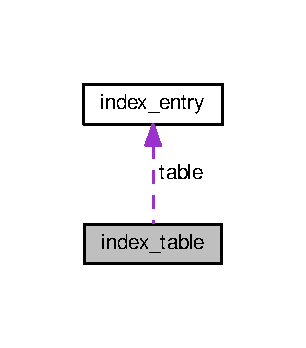
\includegraphics[width=147pt]{structindex__table__coll__graph}
\end{center}
\end{figure}
\subsection*{Data Fields}
\begin{DoxyCompactItemize}
\item 
\hyperlink{structindex__entry}{index\+\_\+entry} \hyperlink{structindex__table_ac79481e508bbe68d18d747f7af369986}{table} \mbox{[}\hyperlink{heap_8h_a032503e76d6f69bc67e99e909c8125da}{T\+A\+B\+L\+E\+\_\+\+S\+I\+ZE}\mbox{]}
\item 
int \hyperlink{structindex__table_a7441ef0865bcb3db9b8064dd7375c1ea}{id}
\end{DoxyCompactItemize}


\subsection{Detailed Description}
Kernel heap index table. 

\subsection{Field Documentation}
\index{index\+\_\+table@{index\+\_\+table}!id@{id}}
\index{id@{id}!index\+\_\+table@{index\+\_\+table}}
\subsubsection[{\texorpdfstring{id}{id}}]{\setlength{\rightskip}{0pt plus 5cm}int id}\hypertarget{structindex__table_a7441ef0865bcb3db9b8064dd7375c1ea}{}\label{structindex__table_a7441ef0865bcb3db9b8064dd7375c1ea}
\index{index\+\_\+table@{index\+\_\+table}!table@{table}}
\index{table@{table}!index\+\_\+table@{index\+\_\+table}}
\subsubsection[{\texorpdfstring{table}{table}}]{\setlength{\rightskip}{0pt plus 5cm}{\bf index\+\_\+entry} table\mbox{[}{\bf T\+A\+B\+L\+E\+\_\+\+S\+I\+ZE}\mbox{]}}\hypertarget{structindex__table_ac79481e508bbe68d18d747f7af369986}{}\label{structindex__table_ac79481e508bbe68d18d747f7af369986}


The documentation for this struct was generated from the following file\+:\begin{DoxyCompactItemize}
\item 
include/mem/\hyperlink{heap_8h}{heap.\+h}\end{DoxyCompactItemize}

\hypertarget{structlmcb}{}\section{lmcb Struct Reference}
\label{structlmcb}\index{lmcb@{lmcb}}


{\ttfamily \#include $<$memory\+Control.\+h$>$}

\subsection*{Data Fields}
\begin{DoxyCompactItemize}
\item 
int \hyperlink{structlmcb_ac765329451135abec74c45e1897abf26}{type}
\item 
int \hyperlink{structlmcb_a439227feff9d7f55384e8780cfc2eb82}{size}
\item 
int \hyperlink{structlmcb_af9658f4d1c59d6d251445c83931f0e55}{mem\+Size}
\end{DoxyCompactItemize}


\subsection{Field Documentation}
\index{lmcb@{lmcb}!mem\+Size@{mem\+Size}}
\index{mem\+Size@{mem\+Size}!lmcb@{lmcb}}
\subsubsection[{\texorpdfstring{mem\+Size}{memSize}}]{\setlength{\rightskip}{0pt plus 5cm}int mem\+Size}\hypertarget{structlmcb_af9658f4d1c59d6d251445c83931f0e55}{}\label{structlmcb_af9658f4d1c59d6d251445c83931f0e55}
\index{lmcb@{lmcb}!size@{size}}
\index{size@{size}!lmcb@{lmcb}}
\subsubsection[{\texorpdfstring{size}{size}}]{\setlength{\rightskip}{0pt plus 5cm}int size}\hypertarget{structlmcb_a439227feff9d7f55384e8780cfc2eb82}{}\label{structlmcb_a439227feff9d7f55384e8780cfc2eb82}
\index{lmcb@{lmcb}!type@{type}}
\index{type@{type}!lmcb@{lmcb}}
\subsubsection[{\texorpdfstring{type}{type}}]{\setlength{\rightskip}{0pt plus 5cm}int type}\hypertarget{structlmcb_ac765329451135abec74c45e1897abf26}{}\label{structlmcb_ac765329451135abec74c45e1897abf26}


The documentation for this struct was generated from the following file\+:\begin{DoxyCompactItemize}
\item 
include/mem/\hyperlink{memory_control_8h}{memory\+Control.\+h}\end{DoxyCompactItemize}

\hypertarget{structnode}{}\section{node Struct Reference}
\label{structnode}\index{node@{node}}


{\ttfamily \#include $<$queue.\+h$>$}



Collaboration diagram for node\+:\nopagebreak
\begin{figure}[H]
\begin{center}
\leavevmode
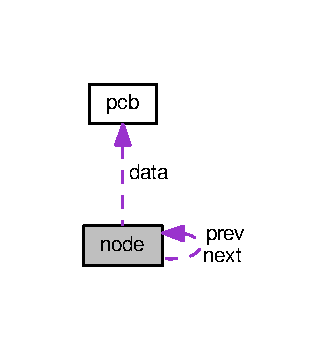
\includegraphics[width=158pt]{structnode__coll__graph}
\end{center}
\end{figure}
\subsection*{Data Fields}
\begin{DoxyCompactItemize}
\item 
struct \hyperlink{structpcb}{pcb} $\ast$ \hyperlink{structnode_a56d819e9a82bb2b5f48ba96fdfe01ca4}{data}
\item 
struct \hyperlink{structnode}{node} $\ast$ \hyperlink{structnode_a0dc1b6470487aa86d9936e3cab8b95be}{next}
\item 
struct \hyperlink{structnode}{node} $\ast$ \hyperlink{structnode_a530843171ca1a6e033bac999737cb184}{prev}
\end{DoxyCompactItemize}


\subsection{Detailed Description}
The struct representing a node in a queue 

\subsection{Field Documentation}
\index{node@{node}!data@{data}}
\index{data@{data}!node@{node}}
\subsubsection[{\texorpdfstring{data}{data}}]{\setlength{\rightskip}{0pt plus 5cm}struct {\bf pcb}$\ast$ data}\hypertarget{structnode_a56d819e9a82bb2b5f48ba96fdfe01ca4}{}\label{structnode_a56d819e9a82bb2b5f48ba96fdfe01ca4}
\index{node@{node}!next@{next}}
\index{next@{next}!node@{node}}
\subsubsection[{\texorpdfstring{next}{next}}]{\setlength{\rightskip}{0pt plus 5cm}struct {\bf node}$\ast$ next}\hypertarget{structnode_a0dc1b6470487aa86d9936e3cab8b95be}{}\label{structnode_a0dc1b6470487aa86d9936e3cab8b95be}
\index{node@{node}!prev@{prev}}
\index{prev@{prev}!node@{node}}
\subsubsection[{\texorpdfstring{prev}{prev}}]{\setlength{\rightskip}{0pt plus 5cm}struct {\bf node}$\ast$ prev}\hypertarget{structnode_a530843171ca1a6e033bac999737cb184}{}\label{structnode_a530843171ca1a6e033bac999737cb184}


The documentation for this struct was generated from the following file\+:\begin{DoxyCompactItemize}
\item 
include/core/\hyperlink{queue_8h}{queue.\+h}\end{DoxyCompactItemize}

\hypertarget{structpage__dir}{}\section{page\+\_\+dir Struct Reference}
\label{structpage__dir}\index{page\+\_\+dir@{page\+\_\+dir}}


{\ttfamily \#include $<$paging.\+h$>$}



Collaboration diagram for page\+\_\+dir\+:\nopagebreak
\begin{figure}[H]
\begin{center}
\leavevmode
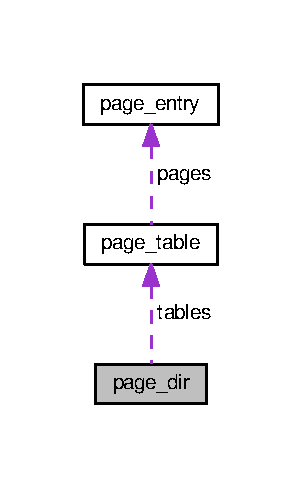
\includegraphics[width=145pt]{structpage__dir__coll__graph}
\end{center}
\end{figure}
\subsection*{Data Fields}
\begin{DoxyCompactItemize}
\item 
\hyperlink{structpage__table}{page\+\_\+table} $\ast$ \hyperlink{structpage__dir_a3d121c0f2d5bf9079178a0889d26ae94}{tables} \mbox{[}1024\mbox{]}
\item 
\hyperlink{system_8h_a757de76cafbcddaac0d1632902fe4cb8}{u32int} \hyperlink{structpage__dir_a67d4c7f42d2b63673971e15ebabed897}{tables\+\_\+phys} \mbox{[}1024\mbox{]}
\end{DoxyCompactItemize}


\subsection{Detailed Description}
Page directory structure Limited to 1024 tables for now 

\subsection{Field Documentation}
\index{page\+\_\+dir@{page\+\_\+dir}!tables@{tables}}
\index{tables@{tables}!page\+\_\+dir@{page\+\_\+dir}}
\subsubsection[{\texorpdfstring{tables}{tables}}]{\setlength{\rightskip}{0pt plus 5cm}{\bf page\+\_\+table}$\ast$ tables\mbox{[}1024\mbox{]}}\hypertarget{structpage__dir_a3d121c0f2d5bf9079178a0889d26ae94}{}\label{structpage__dir_a3d121c0f2d5bf9079178a0889d26ae94}
\index{page\+\_\+dir@{page\+\_\+dir}!tables\+\_\+phys@{tables\+\_\+phys}}
\index{tables\+\_\+phys@{tables\+\_\+phys}!page\+\_\+dir@{page\+\_\+dir}}
\subsubsection[{\texorpdfstring{tables\+\_\+phys}{tables_phys}}]{\setlength{\rightskip}{0pt plus 5cm}{\bf u32int} tables\+\_\+phys\mbox{[}1024\mbox{]}}\hypertarget{structpage__dir_a67d4c7f42d2b63673971e15ebabed897}{}\label{structpage__dir_a67d4c7f42d2b63673971e15ebabed897}


The documentation for this struct was generated from the following file\+:\begin{DoxyCompactItemize}
\item 
include/mem/\hyperlink{paging_8h}{paging.\+h}\end{DoxyCompactItemize}

\hypertarget{structpage__entry}{}\section{page\+\_\+entry Struct Reference}
\label{structpage__entry}\index{page\+\_\+entry@{page\+\_\+entry}}


{\ttfamily \#include $<$paging.\+h$>$}

\subsection*{Data Fields}
\begin{DoxyCompactItemize}
\item 
\hyperlink{system_8h_a757de76cafbcddaac0d1632902fe4cb8}{u32int} \hyperlink{structpage__entry_a69718d61bbe7faf204d90744c9824c52}{present}\+: 1
\item 
\hyperlink{system_8h_a757de76cafbcddaac0d1632902fe4cb8}{u32int} \hyperlink{structpage__entry_a421725c39c0745b022f36ab85b6cf3ce}{writeable}\+: 1
\item 
\hyperlink{system_8h_a757de76cafbcddaac0d1632902fe4cb8}{u32int} \hyperlink{structpage__entry_a277f6a1db251178ac4c5bd2e58acf139}{usermode}\+: 1
\item 
\hyperlink{system_8h_a757de76cafbcddaac0d1632902fe4cb8}{u32int} \hyperlink{structpage__entry_afb99a0327fa4c7332208a4c69586c8ec}{accessed}\+: 1
\item 
\hyperlink{system_8h_a757de76cafbcddaac0d1632902fe4cb8}{u32int} \hyperlink{structpage__entry_a3a32ba260115f27563a8197f17c291a6}{dirty}\+: 1
\item 
\hyperlink{system_8h_a757de76cafbcddaac0d1632902fe4cb8}{u32int} \hyperlink{structpage__entry_a428bdea224227681cbba9cb45f3cca62}{reserved}\+: 7
\item 
\hyperlink{system_8h_a757de76cafbcddaac0d1632902fe4cb8}{u32int} \hyperlink{structpage__entry_a95b631ccb680a6af3d4d4a4fda3ca440}{frameaddr}\+: 20
\end{DoxyCompactItemize}


\subsection{Detailed Description}
Page entry structure Describes a single page in memory 

\subsection{Field Documentation}
\index{page\+\_\+entry@{page\+\_\+entry}!accessed@{accessed}}
\index{accessed@{accessed}!page\+\_\+entry@{page\+\_\+entry}}
\subsubsection[{\texorpdfstring{accessed}{accessed}}]{\setlength{\rightskip}{0pt plus 5cm}{\bf u32int} accessed}\hypertarget{structpage__entry_afb99a0327fa4c7332208a4c69586c8ec}{}\label{structpage__entry_afb99a0327fa4c7332208a4c69586c8ec}
\index{page\+\_\+entry@{page\+\_\+entry}!dirty@{dirty}}
\index{dirty@{dirty}!page\+\_\+entry@{page\+\_\+entry}}
\subsubsection[{\texorpdfstring{dirty}{dirty}}]{\setlength{\rightskip}{0pt plus 5cm}{\bf u32int} dirty}\hypertarget{structpage__entry_a3a32ba260115f27563a8197f17c291a6}{}\label{structpage__entry_a3a32ba260115f27563a8197f17c291a6}
\index{page\+\_\+entry@{page\+\_\+entry}!frameaddr@{frameaddr}}
\index{frameaddr@{frameaddr}!page\+\_\+entry@{page\+\_\+entry}}
\subsubsection[{\texorpdfstring{frameaddr}{frameaddr}}]{\setlength{\rightskip}{0pt plus 5cm}{\bf u32int} frameaddr}\hypertarget{structpage__entry_a95b631ccb680a6af3d4d4a4fda3ca440}{}\label{structpage__entry_a95b631ccb680a6af3d4d4a4fda3ca440}
\index{page\+\_\+entry@{page\+\_\+entry}!present@{present}}
\index{present@{present}!page\+\_\+entry@{page\+\_\+entry}}
\subsubsection[{\texorpdfstring{present}{present}}]{\setlength{\rightskip}{0pt plus 5cm}{\bf u32int} present}\hypertarget{structpage__entry_a69718d61bbe7faf204d90744c9824c52}{}\label{structpage__entry_a69718d61bbe7faf204d90744c9824c52}
\index{page\+\_\+entry@{page\+\_\+entry}!reserved@{reserved}}
\index{reserved@{reserved}!page\+\_\+entry@{page\+\_\+entry}}
\subsubsection[{\texorpdfstring{reserved}{reserved}}]{\setlength{\rightskip}{0pt plus 5cm}{\bf u32int} reserved}\hypertarget{structpage__entry_a428bdea224227681cbba9cb45f3cca62}{}\label{structpage__entry_a428bdea224227681cbba9cb45f3cca62}
\index{page\+\_\+entry@{page\+\_\+entry}!usermode@{usermode}}
\index{usermode@{usermode}!page\+\_\+entry@{page\+\_\+entry}}
\subsubsection[{\texorpdfstring{usermode}{usermode}}]{\setlength{\rightskip}{0pt plus 5cm}{\bf u32int} usermode}\hypertarget{structpage__entry_a277f6a1db251178ac4c5bd2e58acf139}{}\label{structpage__entry_a277f6a1db251178ac4c5bd2e58acf139}
\index{page\+\_\+entry@{page\+\_\+entry}!writeable@{writeable}}
\index{writeable@{writeable}!page\+\_\+entry@{page\+\_\+entry}}
\subsubsection[{\texorpdfstring{writeable}{writeable}}]{\setlength{\rightskip}{0pt plus 5cm}{\bf u32int} writeable}\hypertarget{structpage__entry_a421725c39c0745b022f36ab85b6cf3ce}{}\label{structpage__entry_a421725c39c0745b022f36ab85b6cf3ce}


The documentation for this struct was generated from the following file\+:\begin{DoxyCompactItemize}
\item 
include/mem/\hyperlink{paging_8h}{paging.\+h}\end{DoxyCompactItemize}

\hypertarget{structpage__table}{}\section{page\+\_\+table Struct Reference}
\label{structpage__table}\index{page\+\_\+table@{page\+\_\+table}}


{\ttfamily \#include $<$paging.\+h$>$}



Collaboration diagram for page\+\_\+table\+:\nopagebreak
\begin{figure}[H]
\begin{center}
\leavevmode
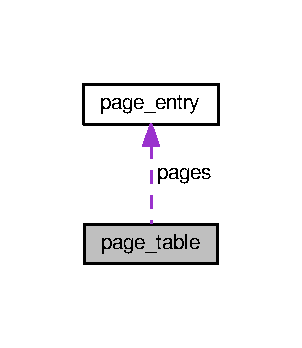
\includegraphics[width=145pt]{structpage__table__coll__graph}
\end{center}
\end{figure}
\subsection*{Data Fields}
\begin{DoxyCompactItemize}
\item 
\hyperlink{structpage__entry}{page\+\_\+entry} \hyperlink{structpage__table_a5cca43bbc67fbbb87eedf886c6e32efb}{pages} \mbox{[}1024\mbox{]}
\end{DoxyCompactItemize}


\subsection{Detailed Description}
Page table structure Contains 1024 pages/frames 

\subsection{Field Documentation}
\index{page\+\_\+table@{page\+\_\+table}!pages@{pages}}
\index{pages@{pages}!page\+\_\+table@{page\+\_\+table}}
\subsubsection[{\texorpdfstring{pages}{pages}}]{\setlength{\rightskip}{0pt plus 5cm}{\bf page\+\_\+entry} pages\mbox{[}1024\mbox{]}}\hypertarget{structpage__table_a5cca43bbc67fbbb87eedf886c6e32efb}{}\label{structpage__table_a5cca43bbc67fbbb87eedf886c6e32efb}


The documentation for this struct was generated from the following file\+:\begin{DoxyCompactItemize}
\item 
include/mem/\hyperlink{paging_8h}{paging.\+h}\end{DoxyCompactItemize}

\hypertarget{structparam}{}\section{param Struct Reference}
\label{structparam}\index{param@{param}}


{\ttfamily \#include $<$mpx\+\_\+supt.\+h$>$}

\subsection*{Data Fields}
\begin{DoxyCompactItemize}
\item 
int \hyperlink{structparam_ab3dee384d0abe30d9ff31e204430241d}{op\+\_\+code}
\item 
int \hyperlink{structparam_accfd0301c469314772cc651ec198d492}{device\+\_\+id}
\end{DoxyCompactItemize}


\subsection{Field Documentation}
\index{param@{param}!device\+\_\+id@{device\+\_\+id}}
\index{device\+\_\+id@{device\+\_\+id}!param@{param}}
\subsubsection[{\texorpdfstring{device\+\_\+id}{device_id}}]{\setlength{\rightskip}{0pt plus 5cm}int device\+\_\+id}\hypertarget{structparam_accfd0301c469314772cc651ec198d492}{}\label{structparam_accfd0301c469314772cc651ec198d492}
\index{param@{param}!op\+\_\+code@{op\+\_\+code}}
\index{op\+\_\+code@{op\+\_\+code}!param@{param}}
\subsubsection[{\texorpdfstring{op\+\_\+code}{op_code}}]{\setlength{\rightskip}{0pt plus 5cm}int op\+\_\+code}\hypertarget{structparam_ab3dee384d0abe30d9ff31e204430241d}{}\label{structparam_ab3dee384d0abe30d9ff31e204430241d}


The documentation for this struct was generated from the following file\+:\begin{DoxyCompactItemize}
\item 
include/modules/\hyperlink{mpx__supt_8h}{mpx\+\_\+supt.\+h}\end{DoxyCompactItemize}

\hypertarget{structpcb}{}\section{pcb Struct Reference}
\label{structpcb}\index{pcb@{pcb}}


{\ttfamily \#include $<$pcb.\+h$>$}

\subsection*{Data Fields}
\begin{DoxyCompactItemize}
\item 
char $\ast$ \hyperlink{structpcb_a87501b25e6cc00b44c763d563ff56feb}{process\+Name}
\item 
int \hyperlink{structpcb_a616049b77d5f877f7cd6633f6c421d63}{process\+Class}
\item 
int \hyperlink{structpcb_acec9ce2df15222151ad66fcb1d74eb9f}{priority}
\item 
int \hyperlink{structpcb_a030f5087a1f437c25cf4a017e8409f49}{is\+Suspended}
\item 
int \hyperlink{structpcb_a89f234133d3efe315836311cbf21c64b}{state}
\item 
unsigned char $\ast$ \hyperlink{structpcb_a4570bd19470baff144028696fa01628c}{stack\+Top}
\item 
unsigned char $\ast$ \hyperlink{structpcb_a02a92960d9b4b330869e1a7bf123f771}{stack\+Bottom}
\end{DoxyCompactItemize}


\subsection{Field Documentation}
\index{pcb@{pcb}!is\+Suspended@{is\+Suspended}}
\index{is\+Suspended@{is\+Suspended}!pcb@{pcb}}
\subsubsection[{\texorpdfstring{is\+Suspended}{isSuspended}}]{\setlength{\rightskip}{0pt plus 5cm}int is\+Suspended}\hypertarget{structpcb_a030f5087a1f437c25cf4a017e8409f49}{}\label{structpcb_a030f5087a1f437c25cf4a017e8409f49}
\index{pcb@{pcb}!priority@{priority}}
\index{priority@{priority}!pcb@{pcb}}
\subsubsection[{\texorpdfstring{priority}{priority}}]{\setlength{\rightskip}{0pt plus 5cm}int priority}\hypertarget{structpcb_acec9ce2df15222151ad66fcb1d74eb9f}{}\label{structpcb_acec9ce2df15222151ad66fcb1d74eb9f}
\index{pcb@{pcb}!process\+Class@{process\+Class}}
\index{process\+Class@{process\+Class}!pcb@{pcb}}
\subsubsection[{\texorpdfstring{process\+Class}{processClass}}]{\setlength{\rightskip}{0pt plus 5cm}int process\+Class}\hypertarget{structpcb_a616049b77d5f877f7cd6633f6c421d63}{}\label{structpcb_a616049b77d5f877f7cd6633f6c421d63}
\index{pcb@{pcb}!process\+Name@{process\+Name}}
\index{process\+Name@{process\+Name}!pcb@{pcb}}
\subsubsection[{\texorpdfstring{process\+Name}{processName}}]{\setlength{\rightskip}{0pt plus 5cm}char$\ast$ process\+Name}\hypertarget{structpcb_a87501b25e6cc00b44c763d563ff56feb}{}\label{structpcb_a87501b25e6cc00b44c763d563ff56feb}
\index{pcb@{pcb}!stack\+Bottom@{stack\+Bottom}}
\index{stack\+Bottom@{stack\+Bottom}!pcb@{pcb}}
\subsubsection[{\texorpdfstring{stack\+Bottom}{stackBottom}}]{\setlength{\rightskip}{0pt plus 5cm}unsigned char$\ast$ stack\+Bottom}\hypertarget{structpcb_a02a92960d9b4b330869e1a7bf123f771}{}\label{structpcb_a02a92960d9b4b330869e1a7bf123f771}
\index{pcb@{pcb}!stack\+Top@{stack\+Top}}
\index{stack\+Top@{stack\+Top}!pcb@{pcb}}
\subsubsection[{\texorpdfstring{stack\+Top}{stackTop}}]{\setlength{\rightskip}{0pt plus 5cm}unsigned char$\ast$ stack\+Top}\hypertarget{structpcb_a4570bd19470baff144028696fa01628c}{}\label{structpcb_a4570bd19470baff144028696fa01628c}
\index{pcb@{pcb}!state@{state}}
\index{state@{state}!pcb@{pcb}}
\subsubsection[{\texorpdfstring{state}{state}}]{\setlength{\rightskip}{0pt plus 5cm}int state}\hypertarget{structpcb_a89f234133d3efe315836311cbf21c64b}{}\label{structpcb_a89f234133d3efe315836311cbf21c64b}


The documentation for this struct was generated from the following file\+:\begin{DoxyCompactItemize}
\item 
include/core/\hyperlink{pcb_8h}{pcb.\+h}\end{DoxyCompactItemize}

\chapter{File Documentation}
\hypertarget{boolean_8h}{}\section{include/boolean.h File Reference}
\label{boolean_8h}\index{include/boolean.\+h@{include/boolean.\+h}}
This graph shows which files directly or indirectly include this file\+:\nopagebreak
\begin{figure}[H]
\begin{center}
\leavevmode
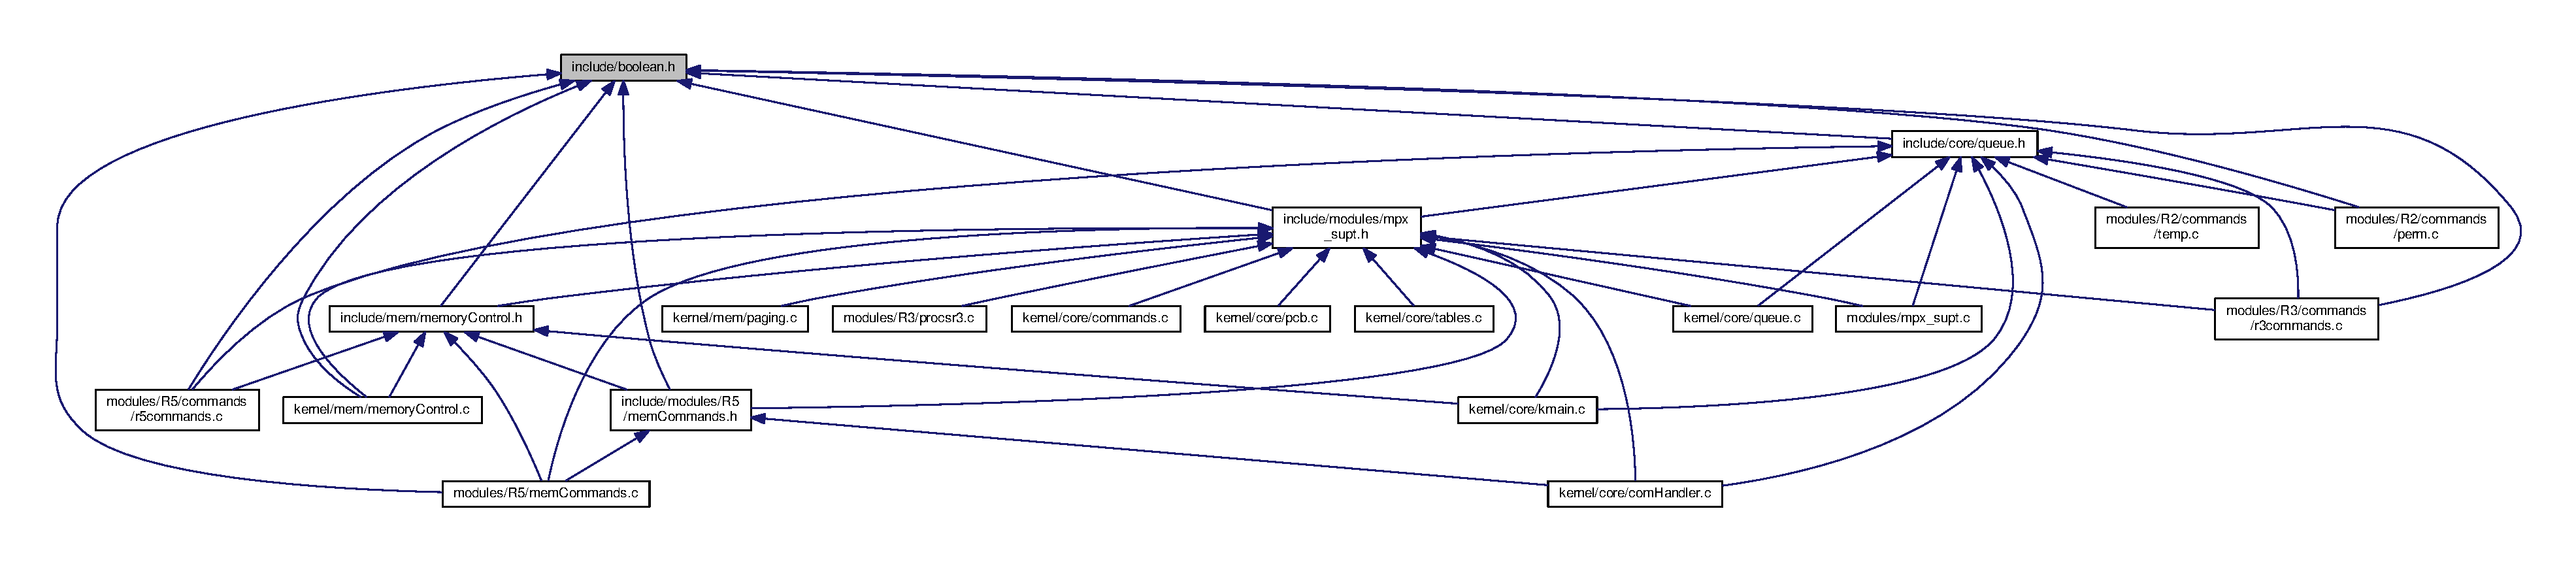
\includegraphics[width=350pt]{boolean_8h__dep__incl}
\end{center}
\end{figure}
\subsection*{Enumerations}
\begin{DoxyCompactItemize}
\item 
enum \hyperlink{boolean_8h_a7c6368b321bd9acd0149b030bb8275ed}{boolean} \{ \hyperlink{boolean_8h_a7c6368b321bd9acd0149b030bb8275edae9de385ef6fe9bf3360d1038396b884c}{false} = 0, 
\hyperlink{boolean_8h_a7c6368b321bd9acd0149b030bb8275eda08f175a5505a10b9ed657defeb050e4b}{true} = 1
 \}
\end{DoxyCompactItemize}


\subsection{Enumeration Type Documentation}
\index{boolean.\+h@{boolean.\+h}!boolean@{boolean}}
\index{boolean@{boolean}!boolean.\+h@{boolean.\+h}}
\subsubsection[{\texorpdfstring{boolean}{boolean}}]{\setlength{\rightskip}{0pt plus 5cm}enum {\bf boolean}}\hypertarget{boolean_8h_a7c6368b321bd9acd0149b030bb8275ed}{}\label{boolean_8h_a7c6368b321bd9acd0149b030bb8275ed}
\begin{Desc}
\item[Enumerator]\par
\begin{description}
\index{false@{false}!boolean.\+h@{boolean.\+h}}\index{boolean.\+h@{boolean.\+h}!false@{false}}\item[{\em 
false\hypertarget{boolean_8h_a7c6368b321bd9acd0149b030bb8275edae9de385ef6fe9bf3360d1038396b884c}{}\label{boolean_8h_a7c6368b321bd9acd0149b030bb8275edae9de385ef6fe9bf3360d1038396b884c}
}]\index{true@{true}!boolean.\+h@{boolean.\+h}}\index{boolean.\+h@{boolean.\+h}!true@{true}}\item[{\em 
true\hypertarget{boolean_8h_a7c6368b321bd9acd0149b030bb8275eda08f175a5505a10b9ed657defeb050e4b}{}\label{boolean_8h_a7c6368b321bd9acd0149b030bb8275eda08f175a5505a10b9ed657defeb050e4b}
}]\end{description}
\end{Desc}

\hypertarget{asm_8h}{}\section{include/core/asm.h File Reference}
\label{asm_8h}\index{include/core/asm.\+h@{include/core/asm.\+h}}
{\ttfamily \#include $<$system.\+h$>$}\\*
{\ttfamily \#include $<$tables.\+h$>$}\\*
Include dependency graph for asm.\+h\+:\nopagebreak
\begin{figure}[H]
\begin{center}
\leavevmode
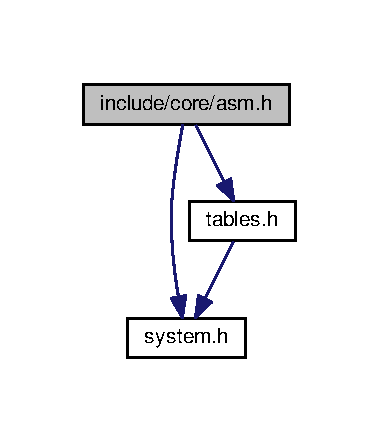
\includegraphics[width=182pt]{asm_8h__incl}
\end{center}
\end{figure}

\hypertarget{com_handler_8h}{}\section{include/core/com\+Handler.h File Reference}
\label{com_handler_8h}\index{include/core/com\+Handler.\+h@{include/core/com\+Handler.\+h}}
{\ttfamily \#include $<$stdint.\+h$>$}\\*
{\ttfamily \#include $<$string.\+h$>$}\\*
{\ttfamily \#include $<$core/io.\+h$>$}\\*
{\ttfamily \#include $<$core/serial.\+h$>$}\\*
Include dependency graph for com\+Handler.\+h\+:\nopagebreak
\begin{figure}[H]
\begin{center}
\leavevmode
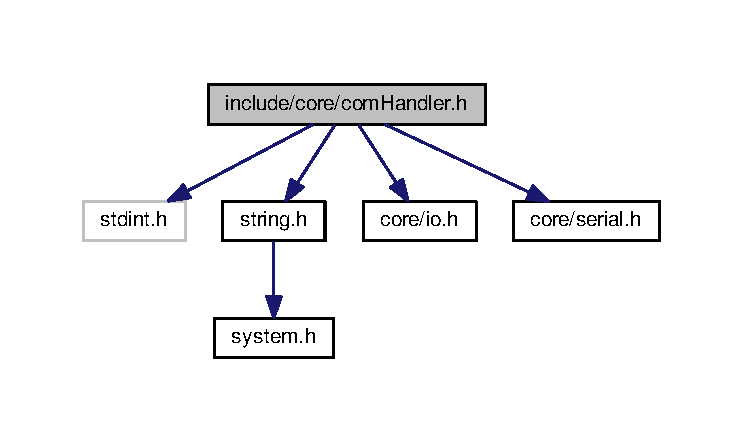
\includegraphics[width=350pt]{com_handler_8h__incl}
\end{center}
\end{figure}
This graph shows which files directly or indirectly include this file\+:\nopagebreak
\begin{figure}[H]
\begin{center}
\leavevmode
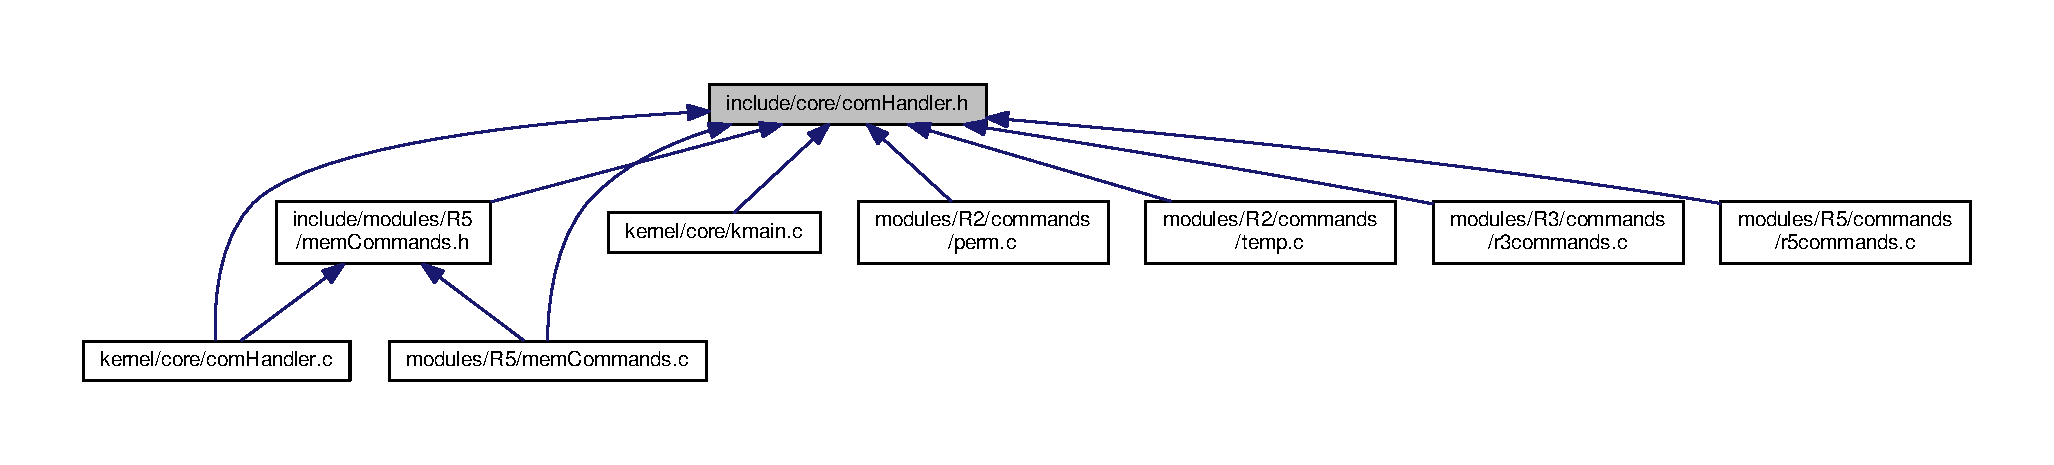
\includegraphics[width=350pt]{com_handler_8h__dep__incl}
\end{center}
\end{figure}
\subsection*{Data Structures}
\begin{DoxyCompactItemize}
\item 
struct \hyperlink{structfunction_def}{function\+Def}
\end{DoxyCompactItemize}
\subsection*{Functions}
\begin{DoxyCompactItemize}
\item 
void \hyperlink{com_handler_8h_af45611c390f08b72ad7f4d38fe845bfa}{add\+Function\+Def} (char $\ast$name, const char $\ast$help\+String, const char $\ast$(func\+Pointer)(char $\ast$$\ast$args, int num\+Args))
\item 
\hyperlink{structfunction_def}{function\+Def} \hyperlink{com_handler_8h_a99dff4fd4af5facdfe9fe8155334c8b6}{get\+Function\+Def} (char $\ast$name)
\item 
const char $\ast$ \hyperlink{com_handler_8h_ae1b11eb92e3c4ef3057c1a2f60d9adcf}{get\+Help\+String} (char $\ast$name)
\item 
char $\ast$ \hyperlink{com_handler_8h_a4621d2e1cae8afd63373d11fd4b8d86e}{get\+Com\+History} (int is\+Prev)
\item 
void \hyperlink{com_handler_8h_ad0ac0a9ea55a932af636e6144c66c4f3}{add\+Com\+History} (char $\ast$new\+Com)
\item 
void \hyperlink{com_handler_8h_a1c6d163609fc84e07bb82328327b7ccb}{print\+Start} ()
\item 
void \hyperlink{com_handler_8h_a097adaa24dfcbf6d84597f5e5e3aea60}{return\+To\+Insertion\+Point} (int end\+Index, int insertion\+Index)
\item 
void \hyperlink{com_handler_8h_adf56ec7300bb290a48fa5c8773950ea2}{erase\+Current\+Row} (int end\+Index, int insertion\+Index)
\item 
char $\ast$ \hyperlink{com_handler_8h_a0701e1cbaa274af91081cdcad3117843}{get\+Input} ()
\item 
void \hyperlink{com_handler_8h_a0b179909cd052ce4a00df79e8a14fbd2}{execute\+Command} (char $\ast$command\+String)
\item 
void \hyperlink{com_handler_8h_a29b919eb7d98b3fc272d7c084437d1ef}{setup\+Commands} ()
\item 
void \hyperlink{com_handler_8h_ae3c8ec1adeb87234023d4b93112397e2}{init\+Command\+Handler} ()
\end{DoxyCompactItemize}


\subsection{Function Documentation}
\index{com\+Handler.\+h@{com\+Handler.\+h}!add\+Com\+History@{add\+Com\+History}}
\index{add\+Com\+History@{add\+Com\+History}!com\+Handler.\+h@{com\+Handler.\+h}}
\subsubsection[{\texorpdfstring{add\+Com\+History(char $\ast$new\+Com)}{addComHistory(char *newCom)}}]{\setlength{\rightskip}{0pt plus 5cm}void add\+Com\+History (
\begin{DoxyParamCaption}
\item[{char $\ast$}]{new\+Com}
\end{DoxyParamCaption}
)}\hypertarget{com_handler_8h_ad0ac0a9ea55a932af636e6144c66c4f3}{}\label{com_handler_8h_ad0ac0a9ea55a932af636e6144c66c4f3}
Helper function to add a command to the command history array


\begin{DoxyParams}{Parameters}
{\em new\+Com} & string to add to the command history \\
\hline
\end{DoxyParams}
\index{com\+Handler.\+h@{com\+Handler.\+h}!add\+Function\+Def@{add\+Function\+Def}}
\index{add\+Function\+Def@{add\+Function\+Def}!com\+Handler.\+h@{com\+Handler.\+h}}
\subsubsection[{\texorpdfstring{add\+Function\+Def(char $\ast$name, const char $\ast$help\+String, const char $\ast$(func\+Pointer)(char $\ast$$\ast$args, int num\+Args))}{addFunctionDef(char *name, const char *helpString, const char *(funcPointer)(char **args, int numArgs))}}]{\setlength{\rightskip}{0pt plus 5cm}void add\+Function\+Def (
\begin{DoxyParamCaption}
\item[{char $\ast$}]{name, }
\item[{const char $\ast$}]{help\+String, }
\item[{const char $\ast$}]{func\+Pointer)(char $\ast$$\ast$args, int num\+Args}
\end{DoxyParamCaption}
)}\hypertarget{com_handler_8h_af45611c390f08b72ad7f4d38fe845bfa}{}\label{com_handler_8h_af45611c390f08b72ad7f4d38fe845bfa}
Adds function definition struct, created from provided params to the function\+Defs array This allows the function to be called in the command handler by its name


\begin{DoxyParams}{Parameters}
{\em name} & -\/ string representation of the function \\
\hline
{\em help\+String} & -\/ const string to be displayed for help \\
\hline
{\em func\+Pointer} & -\/ pointer to the function, must return const char$\ast$ and take in arguments\+: char$\ast$$\ast$ args and int num\+Args \\
\hline
\end{DoxyParams}
\index{com\+Handler.\+h@{com\+Handler.\+h}!erase\+Current\+Row@{erase\+Current\+Row}}
\index{erase\+Current\+Row@{erase\+Current\+Row}!com\+Handler.\+h@{com\+Handler.\+h}}
\subsubsection[{\texorpdfstring{erase\+Current\+Row(int end\+Index, int insertion\+Index)}{eraseCurrentRow(int endIndex, int insertionIndex)}}]{\setlength{\rightskip}{0pt plus 5cm}void erase\+Current\+Row (
\begin{DoxyParamCaption}
\item[{int}]{end\+Index, }
\item[{int}]{insertion\+Index}
\end{DoxyParamCaption}
)}\hypertarget{com_handler_8h_adf56ec7300bb290a48fa5c8773950ea2}{}\label{com_handler_8h_adf56ec7300bb290a48fa5c8773950ea2}
Helper function to remove all printed chars on the current line of input back to the $>$$>$


\begin{DoxyParams}{Parameters}
{\em end\+Index} & -\/ index of last char printed \\
\hline
{\em insertion\+Index} & -\/ index of where insertion point should be \\
\hline
\end{DoxyParams}
\index{com\+Handler.\+h@{com\+Handler.\+h}!execute\+Command@{execute\+Command}}
\index{execute\+Command@{execute\+Command}!com\+Handler.\+h@{com\+Handler.\+h}}
\subsubsection[{\texorpdfstring{execute\+Command(char $\ast$command\+String)}{executeCommand(char *commandString)}}]{\setlength{\rightskip}{0pt plus 5cm}void execute\+Command (
\begin{DoxyParamCaption}
\item[{char $\ast$}]{command\+String}
\end{DoxyParamCaption}
)}\hypertarget{com_handler_8h_a0b179909cd052ce4a00df79e8a14fbd2}{}\label{com_handler_8h_a0b179909cd052ce4a00df79e8a14fbd2}
Gets the command in the given command\+String param and executes it, printing the provided output string


\begin{DoxyParams}{Parameters}
{\em command\+String} & string contianing the command name and any args \\
\hline
\end{DoxyParams}
\index{com\+Handler.\+h@{com\+Handler.\+h}!get\+Com\+History@{get\+Com\+History}}
\index{get\+Com\+History@{get\+Com\+History}!com\+Handler.\+h@{com\+Handler.\+h}}
\subsubsection[{\texorpdfstring{get\+Com\+History(int is\+Prev)}{getComHistory(int isPrev)}}]{\setlength{\rightskip}{0pt plus 5cm}char$\ast$ get\+Com\+History (
\begin{DoxyParamCaption}
\item[{int}]{is\+Prev}
\end{DoxyParamCaption}
)}\hypertarget{com_handler_8h_a4621d2e1cae8afd63373d11fd4b8d86e}{}\label{com_handler_8h_a4621d2e1cae8afd63373d11fd4b8d86e}
Helper function to get the next or previous command from the command history


\begin{DoxyParams}{Parameters}
{\em is\+Prev} & integer denoting if to get the previous command \\
\hline
\end{DoxyParams}
\begin{DoxyReturn}{Returns}
string of the command 
\end{DoxyReturn}
\index{com\+Handler.\+h@{com\+Handler.\+h}!get\+Function\+Def@{get\+Function\+Def}}
\index{get\+Function\+Def@{get\+Function\+Def}!com\+Handler.\+h@{com\+Handler.\+h}}
\subsubsection[{\texorpdfstring{get\+Function\+Def(char $\ast$name)}{getFunctionDef(char *name)}}]{\setlength{\rightskip}{0pt plus 5cm}{\bf function\+Def} get\+Function\+Def (
\begin{DoxyParamCaption}
\item[{char $\ast$}]{name}
\end{DoxyParamCaption}
)}\hypertarget{com_handler_8h_a99dff4fd4af5facdfe9fe8155334c8b6}{}\label{com_handler_8h_a99dff4fd4af5facdfe9fe8155334c8b6}
Gets the \hyperlink{structfunction_def}{function\+Def} struct corresponding to the name provided, returns a \hyperlink{structfunction_def}{function\+Def} with null func\+Pointer if none are found


\begin{DoxyParams}{Parameters}
{\em name} & -\/ name of the \hyperlink{structfunction_def}{function\+Def} \\
\hline
\end{DoxyParams}
\begin{DoxyReturn}{Returns}
\hyperlink{structfunction_def}{function\+Def} 
\end{DoxyReturn}
\index{com\+Handler.\+h@{com\+Handler.\+h}!get\+Help\+String@{get\+Help\+String}}
\index{get\+Help\+String@{get\+Help\+String}!com\+Handler.\+h@{com\+Handler.\+h}}
\subsubsection[{\texorpdfstring{get\+Help\+String(char $\ast$name)}{getHelpString(char *name)}}]{\setlength{\rightskip}{0pt plus 5cm}const char$\ast$ get\+Help\+String (
\begin{DoxyParamCaption}
\item[{char $\ast$}]{name}
\end{DoxyParamCaption}
)}\hypertarget{com_handler_8h_ae1b11eb92e3c4ef3057c1a2f60d9adcf}{}\label{com_handler_8h_ae1b11eb92e3c4ef3057c1a2f60d9adcf}
Gets the help string from the struct for the function name provided


\begin{DoxyParams}{Parameters}
{\em name} & -\/ name associated witht he struct from which to get the help string \\
\hline
\end{DoxyParams}
\begin{DoxyReturn}{Returns}
const char$\ast$ help string 
\end{DoxyReturn}
\index{com\+Handler.\+h@{com\+Handler.\+h}!get\+Input@{get\+Input}}
\index{get\+Input@{get\+Input}!com\+Handler.\+h@{com\+Handler.\+h}}
\subsubsection[{\texorpdfstring{get\+Input()}{getInput()}}]{\setlength{\rightskip}{0pt plus 5cm}char$\ast$ get\+Input (
\begin{DoxyParamCaption}
{}
\end{DoxyParamCaption}
)}\hypertarget{com_handler_8h_a0701e1cbaa274af91081cdcad3117843}{}\label{com_handler_8h_a0701e1cbaa274af91081cdcad3117843}
Polls the input for characters and handles special key strokes such as delete, backspace, arrows, etc. and returns the input string

\begin{DoxyReturn}{Returns}
string that was input 
\end{DoxyReturn}
\index{com\+Handler.\+h@{com\+Handler.\+h}!init\+Command\+Handler@{init\+Command\+Handler}}
\index{init\+Command\+Handler@{init\+Command\+Handler}!com\+Handler.\+h@{com\+Handler.\+h}}
\subsubsection[{\texorpdfstring{init\+Command\+Handler()}{initCommandHandler()}}]{\setlength{\rightskip}{0pt plus 5cm}void init\+Command\+Handler (
\begin{DoxyParamCaption}
{}
\end{DoxyParamCaption}
)}\hypertarget{com_handler_8h_ae3c8ec1adeb87234023d4b93112397e2}{}\label{com_handler_8h_ae3c8ec1adeb87234023d4b93112397e2}
Main function of the com\+Handler that initializes the command handler, continually loops taking in input commands, manages the com\+History, and executes given commands \index{com\+Handler.\+h@{com\+Handler.\+h}!print\+Start@{print\+Start}}
\index{print\+Start@{print\+Start}!com\+Handler.\+h@{com\+Handler.\+h}}
\subsubsection[{\texorpdfstring{print\+Start()}{printStart()}}]{\setlength{\rightskip}{0pt plus 5cm}void print\+Start (
\begin{DoxyParamCaption}
{}
\end{DoxyParamCaption}
)}\hypertarget{com_handler_8h_a1c6d163609fc84e07bb82328327b7ccb}{}\label{com_handler_8h_a1c6d163609fc84e07bb82328327b7ccb}
Helper function to print out the beginning line tag\+: \char`\"{}$>$$>$\char`\"{} \index{com\+Handler.\+h@{com\+Handler.\+h}!return\+To\+Insertion\+Point@{return\+To\+Insertion\+Point}}
\index{return\+To\+Insertion\+Point@{return\+To\+Insertion\+Point}!com\+Handler.\+h@{com\+Handler.\+h}}
\subsubsection[{\texorpdfstring{return\+To\+Insertion\+Point(int end\+Index, int insertion\+Index)}{returnToInsertionPoint(int endIndex, int insertionIndex)}}]{\setlength{\rightskip}{0pt plus 5cm}void return\+To\+Insertion\+Point (
\begin{DoxyParamCaption}
\item[{int}]{end\+Index, }
\item[{int}]{insertion\+Index}
\end{DoxyParamCaption}
)}\hypertarget{com_handler_8h_a097adaa24dfcbf6d84597f5e5e3aea60}{}\label{com_handler_8h_a097adaa24dfcbf6d84597f5e5e3aea60}
Helper function to move the insertion point from the end of the line to the correct placement


\begin{DoxyParams}{Parameters}
{\em end\+Index} & -\/ index of last char printed \\
\hline
{\em insertion\+Index} & -\/ index of where insertion point should be \\
\hline
\end{DoxyParams}
\index{com\+Handler.\+h@{com\+Handler.\+h}!setup\+Commands@{setup\+Commands}}
\index{setup\+Commands@{setup\+Commands}!com\+Handler.\+h@{com\+Handler.\+h}}
\subsubsection[{\texorpdfstring{setup\+Commands()}{setupCommands()}}]{\setlength{\rightskip}{0pt plus 5cm}void setup\+Commands (
\begin{DoxyParamCaption}
{}
\end{DoxyParamCaption}
)}\hypertarget{com_handler_8h_a29b919eb7d98b3fc272d7c084437d1ef}{}\label{com_handler_8h_a29b919eb7d98b3fc272d7c084437d1ef}
Initialization function to add commands ot the function\+Defs array 
\hypertarget{commands_8h}{}\section{include/core/commands.h File Reference}
\label{commands_8h}\index{include/core/commands.\+h@{include/core/commands.\+h}}
This graph shows which files directly or indirectly include this file\+:\nopagebreak
\begin{figure}[H]
\begin{center}
\leavevmode
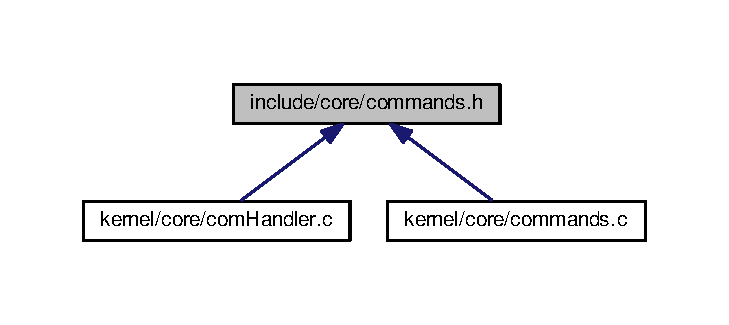
\includegraphics[width=350pt]{commands_8h__dep__incl}
\end{center}
\end{figure}
\subsection*{Functions}
\begin{DoxyCompactItemize}
\item 
const char $\ast$ \hyperlink{commands_8h_a52a5f8d5a6cddf91cd85fb09b8d48dce}{version} (char $\ast$$\ast$args, int num\+Args)
\item 
const char $\ast$ \hyperlink{commands_8h_ab388efb50a8d62df56aa2bcc116a953d}{help} (char $\ast$$\ast$args, int num\+Args)
\item 
const char $\ast$ \hyperlink{commands_8h_afe28183461aff181386fd07baf93bf6d}{shutdown} (char $\ast$$\ast$args, int num\+Args)
\item 
const char $\ast$ \hyperlink{commands_8h_ad9c2acc4a9daa1ebf06b295a4cef9aed}{date} (char $\ast$$\ast$args, int num\+Args)
\end{DoxyCompactItemize}


\subsection{Function Documentation}
\index{commands.\+h@{commands.\+h}!date@{date}}
\index{date@{date}!commands.\+h@{commands.\+h}}
\subsubsection[{\texorpdfstring{date(char $\ast$$\ast$args, int num\+Args)}{date(char **args, int numArgs)}}]{\setlength{\rightskip}{0pt plus 5cm}const char$\ast$ date (
\begin{DoxyParamCaption}
\item[{char $\ast$$\ast$}]{args, }
\item[{int}]{num\+Args}
\end{DoxyParamCaption}
)}\hypertarget{commands_8h_ad9c2acc4a9daa1ebf06b295a4cef9aed}{}\label{commands_8h_ad9c2acc4a9daa1ebf06b295a4cef9aed}
Returns the current date/time in I\+S\+O-\/8601 format. Improperly specified date/times are ignored.

Usage\+: date \mbox{[}--date\mbox{]} \mbox{[}--time\mbox{]} \mbox{[}--setdate yyyy-\/\+M\+M-\/dd\mbox{]} \mbox{[}--settime hh\+:mm\+:ss\mbox{]}

Args\+: \mbox{[}no args\mbox{]} -\/ Return the date and time --date -\/ Return the date --time -\/ Return the time --setdate -\/ Sets the date to the specified date (returns the new date/time) --settime -\/ Sets the time to the specified time (returns the new date/time)


\begin{DoxyParams}{Parameters}
{\em args} & The arguments to pass to the function \\
\hline
{\em num\+Args} & The number of arguments \\
\hline
\end{DoxyParams}
\begin{DoxyReturn}{Returns}
The I\+S\+O-\/8601 formatted date
\end{DoxyReturn}
Returns the current date/time in I\+S\+O-\/8601 format. Improperly specified date/times are ignored.

Usage\+: date \mbox{[}--date\mbox{]} \mbox{[}--time\mbox{]} \mbox{[}--setdate yyyy-\/\+M\+M-\/dd\mbox{]} \mbox{[}--settime hh\+:mm\+:ss\mbox{]}

Args\+: \mbox{[}no args\mbox{]} -\/ Return the date and time --date -\/ Return the date --time -\/ Return the time --setdate -\/ Sets the date to the specified date (returns the new date) --settime -\/ Sets the time to the specified time (returns the new time)


\begin{DoxyParams}{Parameters}
{\em args} & The arguments to pass to the function \\
\hline
\end{DoxyParams}
\begin{DoxyReturn}{Returns}
The I\+S\+O-\/8601 formatted date 
\end{DoxyReturn}
\index{commands.\+h@{commands.\+h}!help@{help}}
\index{help@{help}!commands.\+h@{commands.\+h}}
\subsubsection[{\texorpdfstring{help(char $\ast$$\ast$args, int num\+Args)}{help(char **args, int numArgs)}}]{\setlength{\rightskip}{0pt plus 5cm}const char$\ast$ help (
\begin{DoxyParamCaption}
\item[{char $\ast$$\ast$}]{args, }
\item[{int}]{num\+Args}
\end{DoxyParamCaption}
)}\hypertarget{commands_8h_ab388efb50a8d62df56aa2bcc116a953d}{}\label{commands_8h_ab388efb50a8d62df56aa2bcc116a953d}
Returns help for the specified commands.

Usage\+: help command\+Name

Args\+: \mbox{[}no args\mbox{]} -\/ Returns the help for the help command command\+Name -\/ The name of the command to get help for


\begin{DoxyParams}{Parameters}
{\em args} & The arguments to pass to the function \\
\hline
{\em num\+Args} & The number of arguments \\
\hline
\end{DoxyParams}
\begin{DoxyReturn}{Returns}
The help string 
\end{DoxyReturn}
\index{commands.\+h@{commands.\+h}!shutdown@{shutdown}}
\index{shutdown@{shutdown}!commands.\+h@{commands.\+h}}
\subsubsection[{\texorpdfstring{shutdown(char $\ast$$\ast$args, int num\+Args)}{shutdown(char **args, int numArgs)}}]{\setlength{\rightskip}{0pt plus 5cm}const char$\ast$ shutdown (
\begin{DoxyParamCaption}
\item[{char $\ast$$\ast$}]{args, }
\item[{int}]{num\+Args}
\end{DoxyParamCaption}
)}\hypertarget{commands_8h_afe28183461aff181386fd07baf93bf6d}{}\label{commands_8h_afe28183461aff181386fd07baf93bf6d}
Shuts down the OS after asking for confirmation.

Usage\+: shutdown \mbox{[}--confirm\mbox{]}

Args\+: \mbox{[}no args\mbox{]} -\/ Displays confirmation prompt --confirm -\/ Auto-\/confirms shutdown


\begin{DoxyParams}{Parameters}
{\em args} & The arguments to pass to the function \\
\hline
{\em num\+Args} & The number of arguments \\
\hline
\end{DoxyParams}
\begin{DoxyReturn}{Returns}
True if shutdown was confirmed 
\end{DoxyReturn}
\index{commands.\+h@{commands.\+h}!version@{version}}
\index{version@{version}!commands.\+h@{commands.\+h}}
\subsubsection[{\texorpdfstring{version(char $\ast$$\ast$args, int num\+Args)}{version(char **args, int numArgs)}}]{\setlength{\rightskip}{0pt plus 5cm}const char$\ast$ version (
\begin{DoxyParamCaption}
\item[{char $\ast$$\ast$}]{args, }
\item[{int}]{num\+Args}
\end{DoxyParamCaption}
)}\hypertarget{commands_8h_a52a5f8d5a6cddf91cd85fb09b8d48dce}{}\label{commands_8h_a52a5f8d5a6cddf91cd85fb09b8d48dce}
Returns the current version of the OS.

Usage\+: version

Args\+: \mbox{[}no args\mbox{]} -\/ Returns the version


\begin{DoxyParams}{Parameters}
{\em args} & The arguments to pass to the function \\
\hline
{\em num\+Args} & The number of arguments \\
\hline
\end{DoxyParams}
\begin{DoxyReturn}{Returns}
The version of the OS.
\end{DoxyReturn}
Returns the current version of the OS.

Usage\+: version

Args\+: \mbox{[}no args\mbox{]} -\/ Returns the version


\begin{DoxyParams}{Parameters}
{\em args} & The arguments to pass to the function \\
\hline
\end{DoxyParams}
\begin{DoxyReturn}{Returns}
The version of the OS. 
\end{DoxyReturn}

\hypertarget{core_2help_8h}{}\section{include/core/help.h File Reference}
\label{core_2help_8h}\index{include/core/help.\+h@{include/core/help.\+h}}
This graph shows which files directly or indirectly include this file\+:\nopagebreak
\begin{figure}[H]
\begin{center}
\leavevmode
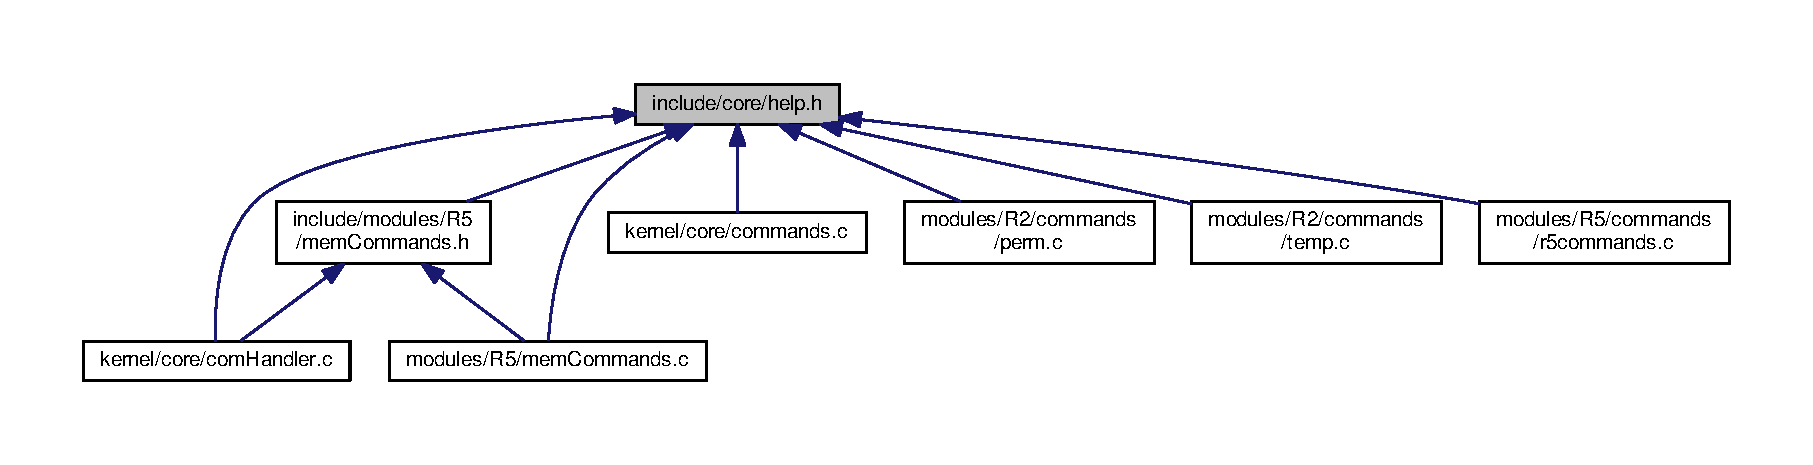
\includegraphics[width=350pt]{core_2help_8h__dep__incl}
\end{center}
\end{figure}
\subsection*{Macros}
\begin{DoxyCompactItemize}
\item 
\#define \hyperlink{core_2help_8h_adf3b9c143880ebac79def26f33303008}{H\+E\+L\+P\+\_\+\+U\+N\+K\+N\+O\+W\+N\+\_\+\+C\+O\+M\+M\+A\+ND}~((const char$\ast$) \char`\"{}Unknown command.\char`\"{})
\item 
\#define \hyperlink{core_2help_8h_a73fc3c00e4bd0fa1f993962853e605d3}{H\+E\+L\+P\+\_\+\+I\+N\+V\+A\+L\+I\+D\+\_\+\+A\+R\+G\+U\+M\+E\+N\+TS}~((const char$\ast$) \char`\"{}Invalid arguments. Please check the documentation for this command.\char`\"{})
\item 
\#define \hyperlink{core_2help_8h_a6a16dbab4e9708f771b676133ec1bbf6}{H\+E\+L\+P\+\_\+\+C\+O\+M\+M\+A\+N\+D\+\_\+\+V\+E\+R\+S\+I\+ON}
\item 
\#define \hyperlink{core_2help_8h_af7d4c48a6c4c03fd0426c81e4fd66b94}{H\+E\+L\+P\+\_\+\+C\+O\+M\+M\+A\+N\+D\+\_\+\+H\+E\+LP}
\item 
\#define \hyperlink{core_2help_8h_a6e574394ffa991934e1adf198fccae08}{H\+E\+L\+P\+\_\+\+C\+O\+M\+M\+A\+N\+D\+\_\+\+S\+H\+U\+T\+D\+O\+WN}
\item 
\#define \hyperlink{core_2help_8h_a44d53654e48f4f20fe33dedf7d847f01}{H\+E\+L\+P\+\_\+\+C\+O\+M\+M\+A\+N\+D\+\_\+\+D\+A\+TE}
\end{DoxyCompactItemize}


\subsection{Macro Definition Documentation}
\index{core/help.\+h@{core/help.\+h}!H\+E\+L\+P\+\_\+\+C\+O\+M\+M\+A\+N\+D\+\_\+\+D\+A\+TE@{H\+E\+L\+P\+\_\+\+C\+O\+M\+M\+A\+N\+D\+\_\+\+D\+A\+TE}}
\index{H\+E\+L\+P\+\_\+\+C\+O\+M\+M\+A\+N\+D\+\_\+\+D\+A\+TE@{H\+E\+L\+P\+\_\+\+C\+O\+M\+M\+A\+N\+D\+\_\+\+D\+A\+TE}!core/help.\+h@{core/help.\+h}}
\subsubsection[{\texorpdfstring{H\+E\+L\+P\+\_\+\+C\+O\+M\+M\+A\+N\+D\+\_\+\+D\+A\+TE}{HELP_COMMAND_DATE}}]{\setlength{\rightskip}{0pt plus 5cm}\#define H\+E\+L\+P\+\_\+\+C\+O\+M\+M\+A\+N\+D\+\_\+\+D\+A\+TE}\hypertarget{core_2help_8h_a44d53654e48f4f20fe33dedf7d847f01}{}\label{core_2help_8h_a44d53654e48f4f20fe33dedf7d847f01}
{\bfseries Value\+:}
\begin{DoxyCode}
((\textcolor{keyword}{const} \textcolor{keywordtype}{char}*) \(\backslash\)
    \textcolor{stringliteral}{"Prints the current date/time in ISO-8601 format.\(\backslash\)n"}\(\backslash\)
    \textcolor{stringliteral}{"Improperly specified date/times are ignored.\(\backslash\)n"}\(\backslash\)
    \textcolor{stringliteral}{"\(\backslash\)n"}\(\backslash\)
    \textcolor{stringliteral}{"Usage: date [--date] [--time] [--setdate yyyy-MM-dd] [--settime hh:mm:ss]\(\backslash\)n"}\(\backslash\)
    \textcolor{stringliteral}{"\(\backslash\)n"}\(\backslash\)
    \textcolor{stringliteral}{"Args:\(\backslash\)n"}\(\backslash\)
    \textcolor{stringliteral}{"    [no args] - Return the date and time\(\backslash\)n"}\(\backslash\)
    \textcolor{stringliteral}{"    --time - Return the time\(\backslash\)n"}\(\backslash\)
    \textcolor{stringliteral}{"    --date - Return the date\(\backslash\)n"}\(\backslash\)
    \textcolor{stringliteral}{"    --setdate - Sets the date to the specified date (returns the new date/time)\(\backslash\)n"}\(\backslash\)
    \textcolor{stringliteral}{"    --settime - Sets the time to the specified time (returns the new date/time)"})
\end{DoxyCode}
\index{core/help.\+h@{core/help.\+h}!H\+E\+L\+P\+\_\+\+C\+O\+M\+M\+A\+N\+D\+\_\+\+H\+E\+LP@{H\+E\+L\+P\+\_\+\+C\+O\+M\+M\+A\+N\+D\+\_\+\+H\+E\+LP}}
\index{H\+E\+L\+P\+\_\+\+C\+O\+M\+M\+A\+N\+D\+\_\+\+H\+E\+LP@{H\+E\+L\+P\+\_\+\+C\+O\+M\+M\+A\+N\+D\+\_\+\+H\+E\+LP}!core/help.\+h@{core/help.\+h}}
\subsubsection[{\texorpdfstring{H\+E\+L\+P\+\_\+\+C\+O\+M\+M\+A\+N\+D\+\_\+\+H\+E\+LP}{HELP_COMMAND_HELP}}]{\setlength{\rightskip}{0pt plus 5cm}\#define H\+E\+L\+P\+\_\+\+C\+O\+M\+M\+A\+N\+D\+\_\+\+H\+E\+LP}\hypertarget{core_2help_8h_af7d4c48a6c4c03fd0426c81e4fd66b94}{}\label{core_2help_8h_af7d4c48a6c4c03fd0426c81e4fd66b94}
{\bfseries Value\+:}
\begin{DoxyCode}
((\textcolor{keyword}{const} \textcolor{keywordtype}{char}*) \(\backslash\)
    \textcolor{stringliteral}{"Prints help for the specified commands.\(\backslash\)n"}\(\backslash\)
    \textcolor{stringliteral}{"\(\backslash\)n"}\(\backslash\)
    \textcolor{stringliteral}{"Usage: help commandName\(\backslash\)n"}\(\backslash\)
    \textcolor{stringliteral}{"\(\backslash\)n"}\(\backslash\)
    \textcolor{stringliteral}{"Args:\(\backslash\)n"}\(\backslash\)
    \textcolor{stringliteral}{"    [no args] - Returns the help for the help command\(\backslash\)n"}\(\backslash\)
    \textcolor{stringliteral}{"    commandName - The name of the command to get help for"})
\end{DoxyCode}
\index{core/help.\+h@{core/help.\+h}!H\+E\+L\+P\+\_\+\+C\+O\+M\+M\+A\+N\+D\+\_\+\+S\+H\+U\+T\+D\+O\+WN@{H\+E\+L\+P\+\_\+\+C\+O\+M\+M\+A\+N\+D\+\_\+\+S\+H\+U\+T\+D\+O\+WN}}
\index{H\+E\+L\+P\+\_\+\+C\+O\+M\+M\+A\+N\+D\+\_\+\+S\+H\+U\+T\+D\+O\+WN@{H\+E\+L\+P\+\_\+\+C\+O\+M\+M\+A\+N\+D\+\_\+\+S\+H\+U\+T\+D\+O\+WN}!core/help.\+h@{core/help.\+h}}
\subsubsection[{\texorpdfstring{H\+E\+L\+P\+\_\+\+C\+O\+M\+M\+A\+N\+D\+\_\+\+S\+H\+U\+T\+D\+O\+WN}{HELP_COMMAND_SHUTDOWN}}]{\setlength{\rightskip}{0pt plus 5cm}\#define H\+E\+L\+P\+\_\+\+C\+O\+M\+M\+A\+N\+D\+\_\+\+S\+H\+U\+T\+D\+O\+WN}\hypertarget{core_2help_8h_a6e574394ffa991934e1adf198fccae08}{}\label{core_2help_8h_a6e574394ffa991934e1adf198fccae08}
{\bfseries Value\+:}
\begin{DoxyCode}
((\textcolor{keyword}{const} \textcolor{keywordtype}{char}*) \(\backslash\)
    \textcolor{stringliteral}{"Shuts down the OS after asking for confirmation.\(\backslash\)n"}\(\backslash\)
    \textcolor{stringliteral}{"\(\backslash\)n"}\(\backslash\)
    \textcolor{stringliteral}{"Usage: shutdown [--confirm]"}\(\backslash\)
    \textcolor{stringliteral}{"\(\backslash\)n"}\(\backslash\)
    \textcolor{stringliteral}{"Args:\(\backslash\)n"}\(\backslash\)
    \textcolor{stringliteral}{"    [no args] - Displays confirmation prompt\(\backslash\)n"}\(\backslash\)
    \textcolor{stringliteral}{"    --confirm - Auto-confirms shutdown"})
\end{DoxyCode}
\index{core/help.\+h@{core/help.\+h}!H\+E\+L\+P\+\_\+\+C\+O\+M\+M\+A\+N\+D\+\_\+\+V\+E\+R\+S\+I\+ON@{H\+E\+L\+P\+\_\+\+C\+O\+M\+M\+A\+N\+D\+\_\+\+V\+E\+R\+S\+I\+ON}}
\index{H\+E\+L\+P\+\_\+\+C\+O\+M\+M\+A\+N\+D\+\_\+\+V\+E\+R\+S\+I\+ON@{H\+E\+L\+P\+\_\+\+C\+O\+M\+M\+A\+N\+D\+\_\+\+V\+E\+R\+S\+I\+ON}!core/help.\+h@{core/help.\+h}}
\subsubsection[{\texorpdfstring{H\+E\+L\+P\+\_\+\+C\+O\+M\+M\+A\+N\+D\+\_\+\+V\+E\+R\+S\+I\+ON}{HELP_COMMAND_VERSION}}]{\setlength{\rightskip}{0pt plus 5cm}\#define H\+E\+L\+P\+\_\+\+C\+O\+M\+M\+A\+N\+D\+\_\+\+V\+E\+R\+S\+I\+ON}\hypertarget{core_2help_8h_a6a16dbab4e9708f771b676133ec1bbf6}{}\label{core_2help_8h_a6a16dbab4e9708f771b676133ec1bbf6}
{\bfseries Value\+:}
\begin{DoxyCode}
((\textcolor{keyword}{const} \textcolor{keywordtype}{char}*) \(\backslash\)
    \textcolor{stringliteral}{"Prints the current version of the OS.\(\backslash\)n"}\(\backslash\)
    \textcolor{stringliteral}{"\(\backslash\)n"}\(\backslash\)
    \textcolor{stringliteral}{"Usage: version\(\backslash\)n"}\(\backslash\)
    \textcolor{stringliteral}{"\(\backslash\)n"}\(\backslash\)
    \textcolor{stringliteral}{"Args:\(\backslash\)n"}\(\backslash\)
    \textcolor{stringliteral}{"    [no args] - Returns the version"})
\end{DoxyCode}
\index{core/help.\+h@{core/help.\+h}!H\+E\+L\+P\+\_\+\+I\+N\+V\+A\+L\+I\+D\+\_\+\+A\+R\+G\+U\+M\+E\+N\+TS@{H\+E\+L\+P\+\_\+\+I\+N\+V\+A\+L\+I\+D\+\_\+\+A\+R\+G\+U\+M\+E\+N\+TS}}
\index{H\+E\+L\+P\+\_\+\+I\+N\+V\+A\+L\+I\+D\+\_\+\+A\+R\+G\+U\+M\+E\+N\+TS@{H\+E\+L\+P\+\_\+\+I\+N\+V\+A\+L\+I\+D\+\_\+\+A\+R\+G\+U\+M\+E\+N\+TS}!core/help.\+h@{core/help.\+h}}
\subsubsection[{\texorpdfstring{H\+E\+L\+P\+\_\+\+I\+N\+V\+A\+L\+I\+D\+\_\+\+A\+R\+G\+U\+M\+E\+N\+TS}{HELP_INVALID_ARGUMENTS}}]{\setlength{\rightskip}{0pt plus 5cm}\#define H\+E\+L\+P\+\_\+\+I\+N\+V\+A\+L\+I\+D\+\_\+\+A\+R\+G\+U\+M\+E\+N\+TS~((const char$\ast$) \char`\"{}Invalid arguments. Please check the documentation for this command.\char`\"{})}\hypertarget{core_2help_8h_a73fc3c00e4bd0fa1f993962853e605d3}{}\label{core_2help_8h_a73fc3c00e4bd0fa1f993962853e605d3}
\index{core/help.\+h@{core/help.\+h}!H\+E\+L\+P\+\_\+\+U\+N\+K\+N\+O\+W\+N\+\_\+\+C\+O\+M\+M\+A\+ND@{H\+E\+L\+P\+\_\+\+U\+N\+K\+N\+O\+W\+N\+\_\+\+C\+O\+M\+M\+A\+ND}}
\index{H\+E\+L\+P\+\_\+\+U\+N\+K\+N\+O\+W\+N\+\_\+\+C\+O\+M\+M\+A\+ND@{H\+E\+L\+P\+\_\+\+U\+N\+K\+N\+O\+W\+N\+\_\+\+C\+O\+M\+M\+A\+ND}!core/help.\+h@{core/help.\+h}}
\subsubsection[{\texorpdfstring{H\+E\+L\+P\+\_\+\+U\+N\+K\+N\+O\+W\+N\+\_\+\+C\+O\+M\+M\+A\+ND}{HELP_UNKNOWN_COMMAND}}]{\setlength{\rightskip}{0pt plus 5cm}\#define H\+E\+L\+P\+\_\+\+U\+N\+K\+N\+O\+W\+N\+\_\+\+C\+O\+M\+M\+A\+ND~((const char$\ast$) \char`\"{}Unknown command.\char`\"{})}\hypertarget{core_2help_8h_adf3b9c143880ebac79def26f33303008}{}\label{core_2help_8h_adf3b9c143880ebac79def26f33303008}

\hypertarget{modules_2_r2_2commands_2help_8h}{}\section{include/modules/\+R2/commands/help.h File Reference}
\label{modules_2_r2_2commands_2help_8h}\index{include/modules/\+R2/commands/help.\+h@{include/modules/\+R2/commands/help.\+h}}
This graph shows which files directly or indirectly include this file\+:\nopagebreak
\begin{figure}[H]
\begin{center}
\leavevmode
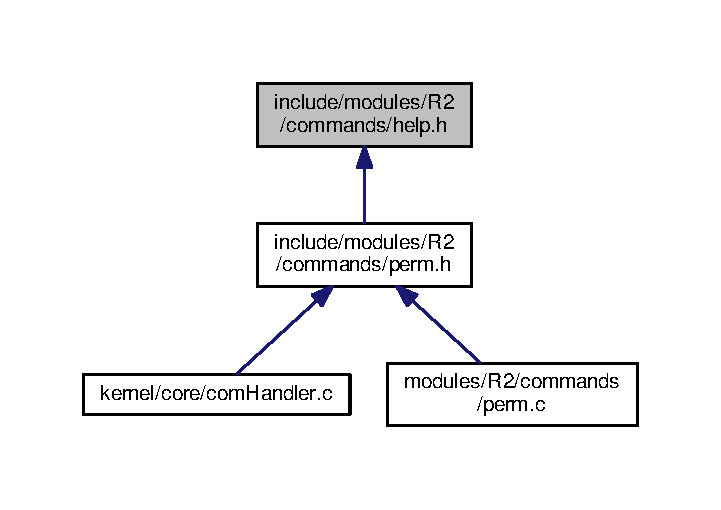
\includegraphics[width=346pt]{modules_2_r2_2commands_2help_8h__dep__incl}
\end{center}
\end{figure}
\subsection*{Macros}
\begin{DoxyCompactItemize}
\item 
\#define \hyperlink{modules_2_r2_2commands_2help_8h_af7e5006fa731a9795f09aef420a2541b}{H\+E\+L\+P\+\_\+\+R2\+\_\+\+C\+O\+M\+M\+A\+N\+D\+\_\+\+S\+P\+CB}
\item 
\#define \hyperlink{modules_2_r2_2commands_2help_8h_ab61e8bf4c5a352d7c16a4862ef9a8eca}{H\+E\+L\+P\+\_\+\+R2\+\_\+\+C\+O\+M\+M\+A\+N\+D\+\_\+\+R\+P\+CB}
\item 
\#define \hyperlink{modules_2_r2_2commands_2help_8h_a082053e40bfb3036b5499019acff2378}{H\+E\+L\+P\+\_\+\+R2\+\_\+\+C\+O\+M\+M\+A\+N\+D\+\_\+\+P\+P\+CB}
\item 
\#define \hyperlink{modules_2_r2_2commands_2help_8h_a212421bf01e8e7c4a28e324d9dc5c501}{H\+E\+L\+P\+\_\+\+R2\+\_\+\+C\+O\+M\+M\+A\+N\+D\+\_\+\+S\+H\+O\+W\+P\+CB}
\end{DoxyCompactItemize}


\subsection{Macro Definition Documentation}
\index{modules/\+R2/commands/help.\+h@{modules/\+R2/commands/help.\+h}!H\+E\+L\+P\+\_\+\+R2\+\_\+\+C\+O\+M\+M\+A\+N\+D\+\_\+\+P\+P\+CB@{H\+E\+L\+P\+\_\+\+R2\+\_\+\+C\+O\+M\+M\+A\+N\+D\+\_\+\+P\+P\+CB}}
\index{H\+E\+L\+P\+\_\+\+R2\+\_\+\+C\+O\+M\+M\+A\+N\+D\+\_\+\+P\+P\+CB@{H\+E\+L\+P\+\_\+\+R2\+\_\+\+C\+O\+M\+M\+A\+N\+D\+\_\+\+P\+P\+CB}!modules/\+R2/commands/help.\+h@{modules/\+R2/commands/help.\+h}}
\subsubsection[{\texorpdfstring{H\+E\+L\+P\+\_\+\+R2\+\_\+\+C\+O\+M\+M\+A\+N\+D\+\_\+\+P\+P\+CB}{HELP_R2_COMMAND_PPCB}}]{\setlength{\rightskip}{0pt plus 5cm}\#define H\+E\+L\+P\+\_\+\+R2\+\_\+\+C\+O\+M\+M\+A\+N\+D\+\_\+\+P\+P\+CB}\hypertarget{modules_2_r2_2commands_2help_8h_a082053e40bfb3036b5499019acff2378}{}\label{modules_2_r2_2commands_2help_8h_a082053e40bfb3036b5499019acff2378}
{\bfseries Value\+:}
\begin{DoxyCode}
((\textcolor{keyword}{const} \textcolor{keywordtype}{char}*) \(\backslash\)
    \textcolor{stringliteral}{"Sets a PCB's priority and reinserts the process into the correct place in the correct queue.\(\backslash\)n"}\(\backslash\)
    \textcolor{stringliteral}{"\(\backslash\)n"}\(\backslash\)
    \textcolor{stringliteral}{"Usage: ppcb name priority\(\backslash\)n"}\(\backslash\)
    \textcolor{stringliteral}{"\(\backslash\)n"}\(\backslash\)
    \textcolor{stringliteral}{"Args:\(\backslash\)n"}\(\backslash\)
    \textcolor{stringliteral}{"    name - The name of the process to set the priority on (must exist)\(\backslash\)n"}\(\backslash\)
    \textcolor{stringliteral}{"    priority - The new priority (between 0 and 9)"})
\end{DoxyCode}
\index{modules/\+R2/commands/help.\+h@{modules/\+R2/commands/help.\+h}!H\+E\+L\+P\+\_\+\+R2\+\_\+\+C\+O\+M\+M\+A\+N\+D\+\_\+\+R\+P\+CB@{H\+E\+L\+P\+\_\+\+R2\+\_\+\+C\+O\+M\+M\+A\+N\+D\+\_\+\+R\+P\+CB}}
\index{H\+E\+L\+P\+\_\+\+R2\+\_\+\+C\+O\+M\+M\+A\+N\+D\+\_\+\+R\+P\+CB@{H\+E\+L\+P\+\_\+\+R2\+\_\+\+C\+O\+M\+M\+A\+N\+D\+\_\+\+R\+P\+CB}!modules/\+R2/commands/help.\+h@{modules/\+R2/commands/help.\+h}}
\subsubsection[{\texorpdfstring{H\+E\+L\+P\+\_\+\+R2\+\_\+\+C\+O\+M\+M\+A\+N\+D\+\_\+\+R\+P\+CB}{HELP_R2_COMMAND_RPCB}}]{\setlength{\rightskip}{0pt plus 5cm}\#define H\+E\+L\+P\+\_\+\+R2\+\_\+\+C\+O\+M\+M\+A\+N\+D\+\_\+\+R\+P\+CB}\hypertarget{modules_2_r2_2commands_2help_8h_ab61e8bf4c5a352d7c16a4862ef9a8eca}{}\label{modules_2_r2_2commands_2help_8h_ab61e8bf4c5a352d7c16a4862ef9a8eca}
{\bfseries Value\+:}
\begin{DoxyCode}
((\textcolor{keyword}{const} \textcolor{keywordtype}{char}*) \(\backslash\)
    \textcolor{stringliteral}{"Places a PCB into the not suspended state and reinserts it into the appropriate queue.\(\backslash\)n"}\(\backslash\)
    \textcolor{stringliteral}{"\(\backslash\)n"}\(\backslash\)
    \textcolor{stringliteral}{"Usage: rpcb name\(\backslash\)n"}\(\backslash\)
    \textcolor{stringliteral}{"\(\backslash\)n"}\(\backslash\)
    \textcolor{stringliteral}{"Args:\(\backslash\)n"}\(\backslash\)
    \textcolor{stringliteral}{"    name - The name of the process to resume (must exist)\(\backslash\)n"}\(\backslash\)
    \textcolor{stringliteral}{"    --all - Resumes all processes"})
\end{DoxyCode}
\index{modules/\+R2/commands/help.\+h@{modules/\+R2/commands/help.\+h}!H\+E\+L\+P\+\_\+\+R2\+\_\+\+C\+O\+M\+M\+A\+N\+D\+\_\+\+S\+H\+O\+W\+P\+CB@{H\+E\+L\+P\+\_\+\+R2\+\_\+\+C\+O\+M\+M\+A\+N\+D\+\_\+\+S\+H\+O\+W\+P\+CB}}
\index{H\+E\+L\+P\+\_\+\+R2\+\_\+\+C\+O\+M\+M\+A\+N\+D\+\_\+\+S\+H\+O\+W\+P\+CB@{H\+E\+L\+P\+\_\+\+R2\+\_\+\+C\+O\+M\+M\+A\+N\+D\+\_\+\+S\+H\+O\+W\+P\+CB}!modules/\+R2/commands/help.\+h@{modules/\+R2/commands/help.\+h}}
\subsubsection[{\texorpdfstring{H\+E\+L\+P\+\_\+\+R2\+\_\+\+C\+O\+M\+M\+A\+N\+D\+\_\+\+S\+H\+O\+W\+P\+CB}{HELP_R2_COMMAND_SHOWPCB}}]{\setlength{\rightskip}{0pt plus 5cm}\#define H\+E\+L\+P\+\_\+\+R2\+\_\+\+C\+O\+M\+M\+A\+N\+D\+\_\+\+S\+H\+O\+W\+P\+CB}\hypertarget{modules_2_r2_2commands_2help_8h_a212421bf01e8e7c4a28e324d9dc5c501}{}\label{modules_2_r2_2commands_2help_8h_a212421bf01e8e7c4a28e324d9dc5c501}
{\bfseries Value\+:}
\begin{DoxyCode}
((\textcolor{keyword}{const} \textcolor{keywordtype}{char}*) \(\backslash\)
    \textcolor{stringliteral}{"Displays the following information for the specified PCBs:\(\backslash\)n"}\(\backslash\)
    \textcolor{stringliteral}{"    Process Name:\(\backslash\)n"}\(\backslash\)
    \textcolor{stringliteral}{"    Class:\(\backslash\)n"}\(\backslash\)
    \textcolor{stringliteral}{"    State:\(\backslash\)n"}\(\backslash\)
    \textcolor{stringliteral}{"    Suspended Status:\(\backslash\)n"}\(\backslash\)
    \textcolor{stringliteral}{"    Priority:\(\backslash\)n"}\(\backslash\)
    \textcolor{stringliteral}{"\(\backslash\)n"}\(\backslash\)
    \textcolor{stringliteral}{"Usage: showpcb [--all] [--ready] [--blocked] [--name pcbName]\(\backslash\)n"}\(\backslash\)
    \textcolor{stringliteral}{"    (at least 1 must be specified)\(\backslash\)n"}\(\backslash\)
    \textcolor{stringliteral}{"\(\backslash\)n"}\(\backslash\)
    \textcolor{stringliteral}{"Args:\(\backslash\)n"}\(\backslash\)
    \textcolor{stringliteral}{"    [no args] - Shows the help for this command\(\backslash\)n"}\(\backslash\)
    \textcolor{stringliteral}{"    --all - Displays information for all PCBs\(\backslash\)n"}\(\backslash\)
    \textcolor{stringliteral}{"    --ready - Displays information for ready PCBs\(\backslash\)n"}\(\backslash\)
    \textcolor{stringliteral}{"    --blocked - Displays information for blocked PCBs\(\backslash\)n"}\(\backslash\)
    \textcolor{stringliteral}{"    --suspended - Displays information for suspended PCBs\(\backslash\)n"}\(\backslash\)
    \textcolor{stringliteral}{"    --name - Displays information for the specified PCB (can be used multiple times)"})
\end{DoxyCode}
\index{modules/\+R2/commands/help.\+h@{modules/\+R2/commands/help.\+h}!H\+E\+L\+P\+\_\+\+R2\+\_\+\+C\+O\+M\+M\+A\+N\+D\+\_\+\+S\+P\+CB@{H\+E\+L\+P\+\_\+\+R2\+\_\+\+C\+O\+M\+M\+A\+N\+D\+\_\+\+S\+P\+CB}}
\index{H\+E\+L\+P\+\_\+\+R2\+\_\+\+C\+O\+M\+M\+A\+N\+D\+\_\+\+S\+P\+CB@{H\+E\+L\+P\+\_\+\+R2\+\_\+\+C\+O\+M\+M\+A\+N\+D\+\_\+\+S\+P\+CB}!modules/\+R2/commands/help.\+h@{modules/\+R2/commands/help.\+h}}
\subsubsection[{\texorpdfstring{H\+E\+L\+P\+\_\+\+R2\+\_\+\+C\+O\+M\+M\+A\+N\+D\+\_\+\+S\+P\+CB}{HELP_R2_COMMAND_SPCB}}]{\setlength{\rightskip}{0pt plus 5cm}\#define H\+E\+L\+P\+\_\+\+R2\+\_\+\+C\+O\+M\+M\+A\+N\+D\+\_\+\+S\+P\+CB}\hypertarget{modules_2_r2_2commands_2help_8h_af7e5006fa731a9795f09aef420a2541b}{}\label{modules_2_r2_2commands_2help_8h_af7e5006fa731a9795f09aef420a2541b}
{\bfseries Value\+:}
\begin{DoxyCode}
((\textcolor{keyword}{const} \textcolor{keywordtype}{char}*) \(\backslash\)
    \textcolor{stringliteral}{"Places a PCB into the suspended state and reinserts it into the appropriate queue.\(\backslash\)n"}\(\backslash\)
    \textcolor{stringliteral}{"\(\backslash\)n"}\(\backslash\)
    \textcolor{stringliteral}{"Usage: spcb name\(\backslash\)n"}\(\backslash\)
    \textcolor{stringliteral}{"\(\backslash\)n"}\(\backslash\)
    \textcolor{stringliteral}{"Args:\(\backslash\)n"}\(\backslash\)
    \textcolor{stringliteral}{"    name - The name of the process to suspend (must exist)"})
\end{DoxyCode}

\hypertarget{modules_2_r3_2commands_2help_8h}{}\section{include/modules/\+R3/commands/help.h File Reference}
\label{modules_2_r3_2commands_2help_8h}\index{include/modules/\+R3/commands/help.\+h@{include/modules/\+R3/commands/help.\+h}}
This graph shows which files directly or indirectly include this file\+:\nopagebreak
\begin{figure}[H]
\begin{center}
\leavevmode
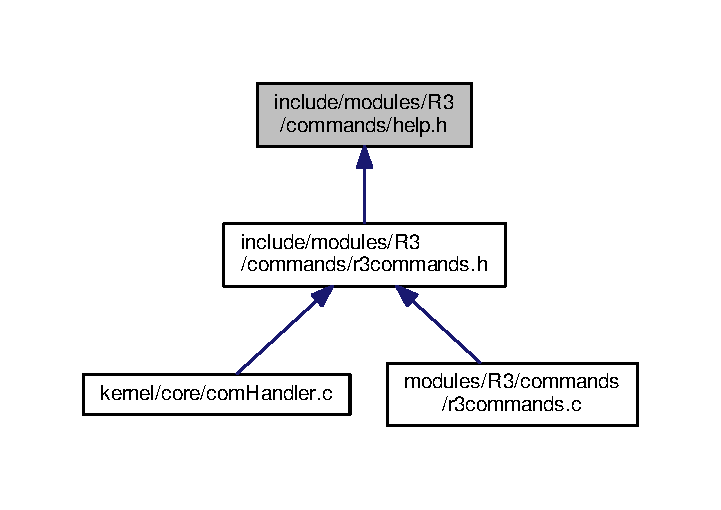
\includegraphics[width=346pt]{modules_2_r3_2commands_2help_8h__dep__incl}
\end{center}
\end{figure}
\subsection*{Macros}
\begin{DoxyCompactItemize}
\item 
\#define \hyperlink{modules_2_r3_2commands_2help_8h_aafd4e68dc4e99af9246c7cc0769306f9}{H\+E\+L\+P\+\_\+\+R3\+\_\+\+C\+O\+M\+M\+A\+N\+D\+\_\+\+Y\+I\+E\+LD}
\item 
\#define \hyperlink{modules_2_r3_2commands_2help_8h_a3a74b43d6f375d35de52752ec24425e9}{H\+E\+L\+P\+\_\+\+R3\+\_\+\+C\+O\+M\+M\+A\+N\+D\+\_\+\+L\+O\+AD}
\end{DoxyCompactItemize}


\subsection{Macro Definition Documentation}
\index{modules/\+R3/commands/help.\+h@{modules/\+R3/commands/help.\+h}!H\+E\+L\+P\+\_\+\+R3\+\_\+\+C\+O\+M\+M\+A\+N\+D\+\_\+\+L\+O\+AD@{H\+E\+L\+P\+\_\+\+R3\+\_\+\+C\+O\+M\+M\+A\+N\+D\+\_\+\+L\+O\+AD}}
\index{H\+E\+L\+P\+\_\+\+R3\+\_\+\+C\+O\+M\+M\+A\+N\+D\+\_\+\+L\+O\+AD@{H\+E\+L\+P\+\_\+\+R3\+\_\+\+C\+O\+M\+M\+A\+N\+D\+\_\+\+L\+O\+AD}!modules/\+R3/commands/help.\+h@{modules/\+R3/commands/help.\+h}}
\subsubsection[{\texorpdfstring{H\+E\+L\+P\+\_\+\+R3\+\_\+\+C\+O\+M\+M\+A\+N\+D\+\_\+\+L\+O\+AD}{HELP_R3_COMMAND_LOAD}}]{\setlength{\rightskip}{0pt plus 5cm}\#define H\+E\+L\+P\+\_\+\+R3\+\_\+\+C\+O\+M\+M\+A\+N\+D\+\_\+\+L\+O\+AD}\hypertarget{modules_2_r3_2commands_2help_8h_a3a74b43d6f375d35de52752ec24425e9}{}\label{modules_2_r3_2commands_2help_8h_a3a74b43d6f375d35de52752ec24425e9}
{\bfseries Value\+:}
\begin{DoxyCode}
((\textcolor{keyword}{const} \textcolor{keywordtype}{char}*) \(\backslash\)
    \textcolor{stringliteral}{"Loads the r3 processes to the queue.\(\backslash\)n"}\(\backslash\)
    \textcolor{stringliteral}{"\(\backslash\)n"}\(\backslash\)
    \textcolor{stringliteral}{"Usage: loadr3\(\backslash\)n"}\(\backslash\)
    \textcolor{stringliteral}{"\(\backslash\)n"}\(\backslash\)
    \textcolor{stringliteral}{"Args:\(\backslash\)n"}\(\backslash\)
    \textcolor{stringliteral}{"    [no args] - loads processes\(\backslash\)n"})
\end{DoxyCode}
\index{modules/\+R3/commands/help.\+h@{modules/\+R3/commands/help.\+h}!H\+E\+L\+P\+\_\+\+R3\+\_\+\+C\+O\+M\+M\+A\+N\+D\+\_\+\+Y\+I\+E\+LD@{H\+E\+L\+P\+\_\+\+R3\+\_\+\+C\+O\+M\+M\+A\+N\+D\+\_\+\+Y\+I\+E\+LD}}
\index{H\+E\+L\+P\+\_\+\+R3\+\_\+\+C\+O\+M\+M\+A\+N\+D\+\_\+\+Y\+I\+E\+LD@{H\+E\+L\+P\+\_\+\+R3\+\_\+\+C\+O\+M\+M\+A\+N\+D\+\_\+\+Y\+I\+E\+LD}!modules/\+R3/commands/help.\+h@{modules/\+R3/commands/help.\+h}}
\subsubsection[{\texorpdfstring{H\+E\+L\+P\+\_\+\+R3\+\_\+\+C\+O\+M\+M\+A\+N\+D\+\_\+\+Y\+I\+E\+LD}{HELP_R3_COMMAND_YIELD}}]{\setlength{\rightskip}{0pt plus 5cm}\#define H\+E\+L\+P\+\_\+\+R3\+\_\+\+C\+O\+M\+M\+A\+N\+D\+\_\+\+Y\+I\+E\+LD}\hypertarget{modules_2_r3_2commands_2help_8h_aafd4e68dc4e99af9246c7cc0769306f9}{}\label{modules_2_r3_2commands_2help_8h_aafd4e68dc4e99af9246c7cc0769306f9}
{\bfseries Value\+:}
\begin{DoxyCode}
((\textcolor{keyword}{const} \textcolor{keywordtype}{char}*) \(\backslash\)
    \textcolor{stringliteral}{"Yields command handler to allow other processes to run.\(\backslash\)n"}\(\backslash\)
    \textcolor{stringliteral}{"\(\backslash\)n"}\(\backslash\)
    \textcolor{stringliteral}{"Usage: yield\(\backslash\)n"}\(\backslash\)
    \textcolor{stringliteral}{"\(\backslash\)n"}\(\backslash\)
    \textcolor{stringliteral}{"Args:\(\backslash\)n"}\(\backslash\)
    \textcolor{stringliteral}{"    [no args] - yields command handler\(\backslash\)n"})
\end{DoxyCode}

\hypertarget{modules_2_r5_2commands_2help_8h}{}\section{include/modules/\+R5/commands/help.h File Reference}
\label{modules_2_r5_2commands_2help_8h}\index{include/modules/\+R5/commands/help.\+h@{include/modules/\+R5/commands/help.\+h}}
This graph shows which files directly or indirectly include this file\+:\nopagebreak
\begin{figure}[H]
\begin{center}
\leavevmode
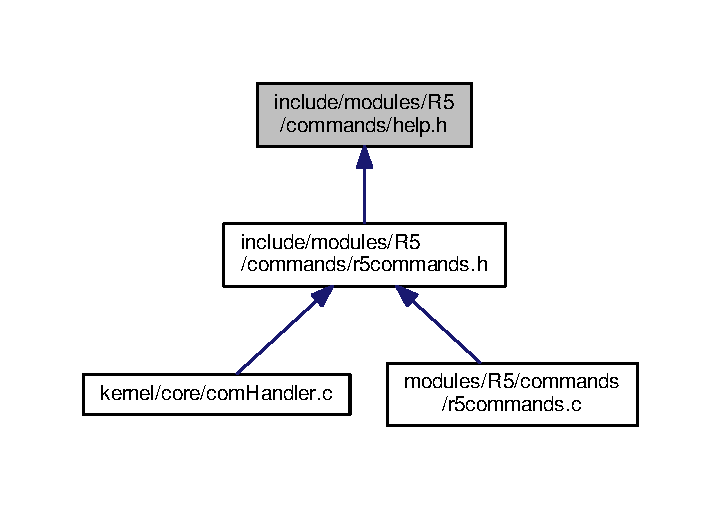
\includegraphics[width=346pt]{modules_2_r5_2commands_2help_8h__dep__incl}
\end{center}
\end{figure}
\subsection*{Macros}
\begin{DoxyCompactItemize}
\item 
\#define \hyperlink{modules_2_r5_2commands_2help_8h_a843ccaf39356ca6188956e9901c57eec}{H\+E\+L\+P\+\_\+\+R5\+\_\+\+C\+O\+M\+M\+A\+N\+D\+\_\+\+S\+H\+O\+W\+M\+E\+M\+O\+RY}
\end{DoxyCompactItemize}


\subsection{Macro Definition Documentation}
\index{modules/\+R5/commands/help.\+h@{modules/\+R5/commands/help.\+h}!H\+E\+L\+P\+\_\+\+R5\+\_\+\+C\+O\+M\+M\+A\+N\+D\+\_\+\+S\+H\+O\+W\+M\+E\+M\+O\+RY@{H\+E\+L\+P\+\_\+\+R5\+\_\+\+C\+O\+M\+M\+A\+N\+D\+\_\+\+S\+H\+O\+W\+M\+E\+M\+O\+RY}}
\index{H\+E\+L\+P\+\_\+\+R5\+\_\+\+C\+O\+M\+M\+A\+N\+D\+\_\+\+S\+H\+O\+W\+M\+E\+M\+O\+RY@{H\+E\+L\+P\+\_\+\+R5\+\_\+\+C\+O\+M\+M\+A\+N\+D\+\_\+\+S\+H\+O\+W\+M\+E\+M\+O\+RY}!modules/\+R5/commands/help.\+h@{modules/\+R5/commands/help.\+h}}
\subsubsection[{\texorpdfstring{H\+E\+L\+P\+\_\+\+R5\+\_\+\+C\+O\+M\+M\+A\+N\+D\+\_\+\+S\+H\+O\+W\+M\+E\+M\+O\+RY}{HELP_R5_COMMAND_SHOWMEMORY}}]{\setlength{\rightskip}{0pt plus 5cm}\#define H\+E\+L\+P\+\_\+\+R5\+\_\+\+C\+O\+M\+M\+A\+N\+D\+\_\+\+S\+H\+O\+W\+M\+E\+M\+O\+RY}\hypertarget{modules_2_r5_2commands_2help_8h_a843ccaf39356ca6188956e9901c57eec}{}\label{modules_2_r5_2commands_2help_8h_a843ccaf39356ca6188956e9901c57eec}
{\bfseries Value\+:}
\begin{DoxyCode}
((\textcolor{keyword}{const} \textcolor{keywordtype}{char}*) \(\backslash\)
    \textcolor{stringliteral}{"Displays the following information for the specified CMCB's:\(\backslash\)n"}\(\backslash\)
    \textcolor{stringliteral}{"CMCB Type:\(\backslash\)n"}\(\backslash\)
    \textcolor{stringliteral}{"Begining Memory Address:\(\backslash\)n"}\(\backslash\)
    \textcolor{stringliteral}{"Block Size:\(\backslash\)n"}\(\backslash\)
    \textcolor{stringliteral}{"Memory Size:\(\backslash\)n"}\(\backslash\)
    \textcolor{stringliteral}{"Process Name:\(\backslash\)n"}\(\backslash\)
    \textcolor{stringliteral}{"\(\backslash\)n"}\(\backslash\)
    \textcolor{stringliteral}{"Usage: showMemory [--all] [--free] [--allocated]\(\backslash\)n"}\(\backslash\)
    \textcolor{stringliteral}{"\(\backslash\)n"}\(\backslash\)
    \textcolor{stringliteral}{"Args:\(\backslash\)n"}\(\backslash\)
    \textcolor{stringliteral}{"    [no args] - Shows the help for this command\(\backslash\)n"}\(\backslash\)
    \textcolor{stringliteral}{"    --all - Displays both free and allocated memory\(\backslash\)n"}\(\backslash\)
    \textcolor{stringliteral}{"    --free - Displays free memory\(\backslash\)n"}\(\backslash\)
    \textcolor{stringliteral}{"    --allocated - Displays allocated memory"})
\end{DoxyCode}

\hypertarget{modules_2_r5_2help_8h}{}\section{include/modules/\+R5/help.h File Reference}
\label{modules_2_r5_2help_8h}\index{include/modules/\+R5/help.\+h@{include/modules/\+R5/help.\+h}}
This graph shows which files directly or indirectly include this file\+:\nopagebreak
\begin{figure}[H]
\begin{center}
\leavevmode
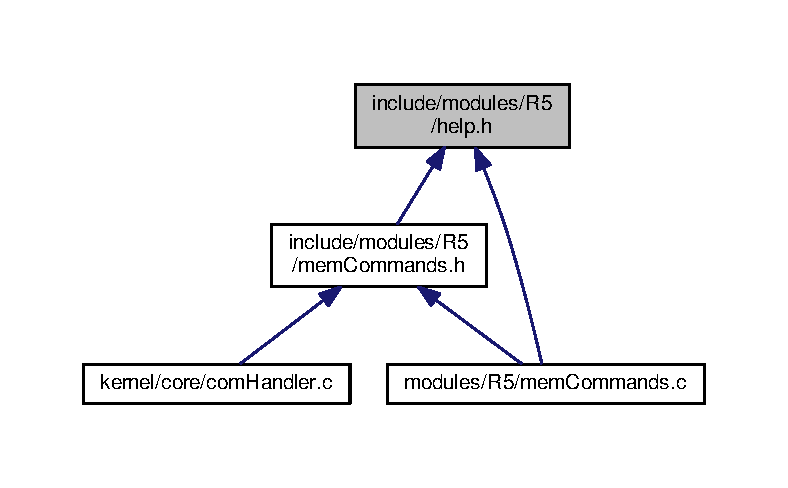
\includegraphics[width=350pt]{modules_2_r5_2help_8h__dep__incl}
\end{center}
\end{figure}
\subsection*{Macros}
\begin{DoxyCompactItemize}
\item 
\#define \hyperlink{modules_2_r5_2help_8h_a40b23c2d24bedc315c563b5a30c0099c}{H\+E\+L\+P\+\_\+\+R5\+\_\+\+C\+O\+M\+M\+A\+N\+D\+\_\+\+H\+E\+AP}
\item 
\#define \hyperlink{modules_2_r5_2help_8h_a83824e1988f7602b0a49a2e445687c9b}{H\+E\+L\+P\+\_\+\+R5\+\_\+\+C\+O\+M\+M\+A\+N\+D\+\_\+\+A\+L\+L\+OC}
\item 
\#define \hyperlink{modules_2_r5_2help_8h_a965bf83361e8b03762b0aa6ac079fb12}{H\+E\+L\+P\+\_\+\+R5\+\_\+\+C\+O\+M\+M\+A\+N\+D\+\_\+\+F\+R\+EE}
\item 
\#define \hyperlink{modules_2_r5_2help_8h_a63cdbbdd3d0ffc3fd74f781779298fe8}{H\+E\+L\+P\+\_\+\+R5\+\_\+\+C\+O\+M\+M\+A\+N\+D\+\_\+\+E\+M\+P\+TY}
\end{DoxyCompactItemize}


\subsection{Macro Definition Documentation}
\index{modules/\+R5/help.\+h@{modules/\+R5/help.\+h}!H\+E\+L\+P\+\_\+\+R5\+\_\+\+C\+O\+M\+M\+A\+N\+D\+\_\+\+A\+L\+L\+OC@{H\+E\+L\+P\+\_\+\+R5\+\_\+\+C\+O\+M\+M\+A\+N\+D\+\_\+\+A\+L\+L\+OC}}
\index{H\+E\+L\+P\+\_\+\+R5\+\_\+\+C\+O\+M\+M\+A\+N\+D\+\_\+\+A\+L\+L\+OC@{H\+E\+L\+P\+\_\+\+R5\+\_\+\+C\+O\+M\+M\+A\+N\+D\+\_\+\+A\+L\+L\+OC}!modules/\+R5/help.\+h@{modules/\+R5/help.\+h}}
\subsubsection[{\texorpdfstring{H\+E\+L\+P\+\_\+\+R5\+\_\+\+C\+O\+M\+M\+A\+N\+D\+\_\+\+A\+L\+L\+OC}{HELP_R5_COMMAND_ALLOC}}]{\setlength{\rightskip}{0pt plus 5cm}\#define H\+E\+L\+P\+\_\+\+R5\+\_\+\+C\+O\+M\+M\+A\+N\+D\+\_\+\+A\+L\+L\+OC}\hypertarget{modules_2_r5_2help_8h_a83824e1988f7602b0a49a2e445687c9b}{}\label{modules_2_r5_2help_8h_a83824e1988f7602b0a49a2e445687c9b}
{\bfseries Value\+:}
\begin{DoxyCode}
((\textcolor{keyword}{const} \textcolor{keywordtype}{char}*) \(\backslash\)
    \textcolor{stringliteral}{"Allocates memory block if memory is available\(\backslash\)n"}\(\backslash\)
    \textcolor{stringliteral}{"\(\backslash\)n"}\(\backslash\)
    \textcolor{stringliteral}{"Usage: allocMem size\(\backslash\)n"}\(\backslash\)
    \textcolor{stringliteral}{"\(\backslash\)n"}\(\backslash\)
    \textcolor{stringliteral}{"Args:\(\backslash\)n"}\(\backslash\)
    \textcolor{stringliteral}{"    size - The size of the memory in bytes"})
\end{DoxyCode}
\index{modules/\+R5/help.\+h@{modules/\+R5/help.\+h}!H\+E\+L\+P\+\_\+\+R5\+\_\+\+C\+O\+M\+M\+A\+N\+D\+\_\+\+E\+M\+P\+TY@{H\+E\+L\+P\+\_\+\+R5\+\_\+\+C\+O\+M\+M\+A\+N\+D\+\_\+\+E\+M\+P\+TY}}
\index{H\+E\+L\+P\+\_\+\+R5\+\_\+\+C\+O\+M\+M\+A\+N\+D\+\_\+\+E\+M\+P\+TY@{H\+E\+L\+P\+\_\+\+R5\+\_\+\+C\+O\+M\+M\+A\+N\+D\+\_\+\+E\+M\+P\+TY}!modules/\+R5/help.\+h@{modules/\+R5/help.\+h}}
\subsubsection[{\texorpdfstring{H\+E\+L\+P\+\_\+\+R5\+\_\+\+C\+O\+M\+M\+A\+N\+D\+\_\+\+E\+M\+P\+TY}{HELP_R5_COMMAND_EMPTY}}]{\setlength{\rightskip}{0pt plus 5cm}\#define H\+E\+L\+P\+\_\+\+R5\+\_\+\+C\+O\+M\+M\+A\+N\+D\+\_\+\+E\+M\+P\+TY}\hypertarget{modules_2_r5_2help_8h_a63cdbbdd3d0ffc3fd74f781779298fe8}{}\label{modules_2_r5_2help_8h_a63cdbbdd3d0ffc3fd74f781779298fe8}
{\bfseries Value\+:}
\begin{DoxyCode}
((\textcolor{keyword}{const} \textcolor{keywordtype}{char}*) \(\backslash\)
    \textcolor{stringliteral}{"Checks if memory is empty\(\backslash\)n"}\(\backslash\)
    \textcolor{stringliteral}{"\(\backslash\)n"}\(\backslash\)
    \textcolor{stringliteral}{"Usage: isEmpty \(\backslash\)n"}\(\backslash\)
    \textcolor{stringliteral}{"\(\backslash\)n"}\(\backslash\)
    \textcolor{stringliteral}{"Args:\(\backslash\)n"}\(\backslash\)
    \textcolor{stringliteral}{"    "})
\end{DoxyCode}
\index{modules/\+R5/help.\+h@{modules/\+R5/help.\+h}!H\+E\+L\+P\+\_\+\+R5\+\_\+\+C\+O\+M\+M\+A\+N\+D\+\_\+\+F\+R\+EE@{H\+E\+L\+P\+\_\+\+R5\+\_\+\+C\+O\+M\+M\+A\+N\+D\+\_\+\+F\+R\+EE}}
\index{H\+E\+L\+P\+\_\+\+R5\+\_\+\+C\+O\+M\+M\+A\+N\+D\+\_\+\+F\+R\+EE@{H\+E\+L\+P\+\_\+\+R5\+\_\+\+C\+O\+M\+M\+A\+N\+D\+\_\+\+F\+R\+EE}!modules/\+R5/help.\+h@{modules/\+R5/help.\+h}}
\subsubsection[{\texorpdfstring{H\+E\+L\+P\+\_\+\+R5\+\_\+\+C\+O\+M\+M\+A\+N\+D\+\_\+\+F\+R\+EE}{HELP_R5_COMMAND_FREE}}]{\setlength{\rightskip}{0pt plus 5cm}\#define H\+E\+L\+P\+\_\+\+R5\+\_\+\+C\+O\+M\+M\+A\+N\+D\+\_\+\+F\+R\+EE}\hypertarget{modules_2_r5_2help_8h_a965bf83361e8b03762b0aa6ac079fb12}{}\label{modules_2_r5_2help_8h_a965bf83361e8b03762b0aa6ac079fb12}
{\bfseries Value\+:}
\begin{DoxyCode}
((\textcolor{keyword}{const} \textcolor{keywordtype}{char}*) \(\backslash\)
    \textcolor{stringliteral}{"Free up memory the memory at the given address\(\backslash\)n"}\(\backslash\)
    \textcolor{stringliteral}{"\(\backslash\)n"}\(\backslash\)
    \textcolor{stringliteral}{"Usage: freeMem address\(\backslash\)n"}\(\backslash\)
    \textcolor{stringliteral}{"\(\backslash\)n"}\(\backslash\)
    \textcolor{stringliteral}{"Args:\(\backslash\)n"}\(\backslash\)
    \textcolor{stringliteral}{"    address - the integer address of the memory"})
\end{DoxyCode}
\index{modules/\+R5/help.\+h@{modules/\+R5/help.\+h}!H\+E\+L\+P\+\_\+\+R5\+\_\+\+C\+O\+M\+M\+A\+N\+D\+\_\+\+H\+E\+AP@{H\+E\+L\+P\+\_\+\+R5\+\_\+\+C\+O\+M\+M\+A\+N\+D\+\_\+\+H\+E\+AP}}
\index{H\+E\+L\+P\+\_\+\+R5\+\_\+\+C\+O\+M\+M\+A\+N\+D\+\_\+\+H\+E\+AP@{H\+E\+L\+P\+\_\+\+R5\+\_\+\+C\+O\+M\+M\+A\+N\+D\+\_\+\+H\+E\+AP}!modules/\+R5/help.\+h@{modules/\+R5/help.\+h}}
\subsubsection[{\texorpdfstring{H\+E\+L\+P\+\_\+\+R5\+\_\+\+C\+O\+M\+M\+A\+N\+D\+\_\+\+H\+E\+AP}{HELP_R5_COMMAND_HEAP}}]{\setlength{\rightskip}{0pt plus 5cm}\#define H\+E\+L\+P\+\_\+\+R5\+\_\+\+C\+O\+M\+M\+A\+N\+D\+\_\+\+H\+E\+AP}\hypertarget{modules_2_r5_2help_8h_a40b23c2d24bedc315c563b5a30c0099c}{}\label{modules_2_r5_2help_8h_a40b23c2d24bedc315c563b5a30c0099c}
{\bfseries Value\+:}
\begin{DoxyCode}
((\textcolor{keyword}{const} \textcolor{keywordtype}{char}*) \(\backslash\)
    \textcolor{stringliteral}{"Initializes the heap\(\backslash\)n"}\(\backslash\)
    \textcolor{stringliteral}{"\(\backslash\)n"}\(\backslash\)
    \textcolor{stringliteral}{"Usage: initHeap size\(\backslash\)n"}\(\backslash\)
    \textcolor{stringliteral}{"\(\backslash\)n"}\(\backslash\)
    \textcolor{stringliteral}{"Args:\(\backslash\)n"}\(\backslash\)
    \textcolor{stringliteral}{"    size - The size of the heap in bytes "})
\end{DoxyCode}

\hypertarget{interrupts_8h}{}\section{include/core/interrupts.h File Reference}
\label{interrupts_8h}\index{include/core/interrupts.\+h@{include/core/interrupts.\+h}}
This graph shows which files directly or indirectly include this file\+:\nopagebreak
\begin{figure}[H]
\begin{center}
\leavevmode
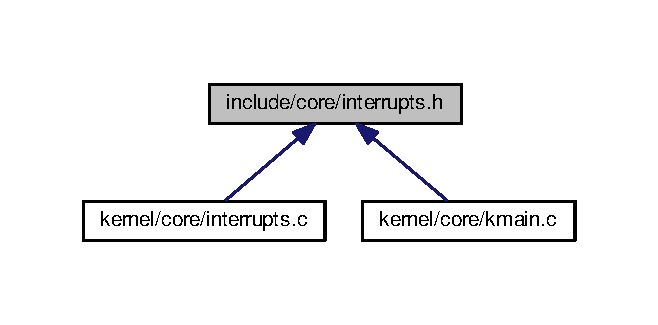
\includegraphics[width=316pt]{interrupts_8h__dep__incl}
\end{center}
\end{figure}
\subsection*{Functions}
\begin{DoxyCompactItemize}
\item 
void \hyperlink{interrupts_8h_ad17d9a8aa78440af8fc40d3fd55dbad8}{init\+\_\+irq} (void)
\item 
void \hyperlink{interrupts_8h_afbc0dbef6f15e2df21b38724ea38c483}{init\+\_\+pic} (void)
\end{DoxyCompactItemize}


\subsection{Function Documentation}
\index{interrupts.\+h@{interrupts.\+h}!init\+\_\+irq@{init\+\_\+irq}}
\index{init\+\_\+irq@{init\+\_\+irq}!interrupts.\+h@{interrupts.\+h}}
\subsubsection[{\texorpdfstring{init\+\_\+irq(void)}{init_irq(void)}}]{\setlength{\rightskip}{0pt plus 5cm}void init\+\_\+irq (
\begin{DoxyParamCaption}
\item[{void}]{}
\end{DoxyParamCaption}
)}\hypertarget{interrupts_8h_ad17d9a8aa78440af8fc40d3fd55dbad8}{}\label{interrupts_8h_ad17d9a8aa78440af8fc40d3fd55dbad8}
Installs the initial interrupt handlers for the first 32 irq lines. Most do a panic for now. \index{interrupts.\+h@{interrupts.\+h}!init\+\_\+pic@{init\+\_\+pic}}
\index{init\+\_\+pic@{init\+\_\+pic}!interrupts.\+h@{interrupts.\+h}}
\subsubsection[{\texorpdfstring{init\+\_\+pic(void)}{init_pic(void)}}]{\setlength{\rightskip}{0pt plus 5cm}void init\+\_\+pic (
\begin{DoxyParamCaption}
\item[{void}]{}
\end{DoxyParamCaption}
)}\hypertarget{interrupts_8h_afbc0dbef6f15e2df21b38724ea38c483}{}\label{interrupts_8h_afbc0dbef6f15e2df21b38724ea38c483}
Initializes the programmable interrupt controllers and performs the necessary remapping of I\+R\+Qs. Leaves interrupts turned off. 
\hypertarget{io_8h}{}\section{include/core/io.h File Reference}
\label{io_8h}\index{include/core/io.\+h@{include/core/io.\+h}}
This graph shows which files directly or indirectly include this file\+:\nopagebreak
\begin{figure}[H]
\begin{center}
\leavevmode
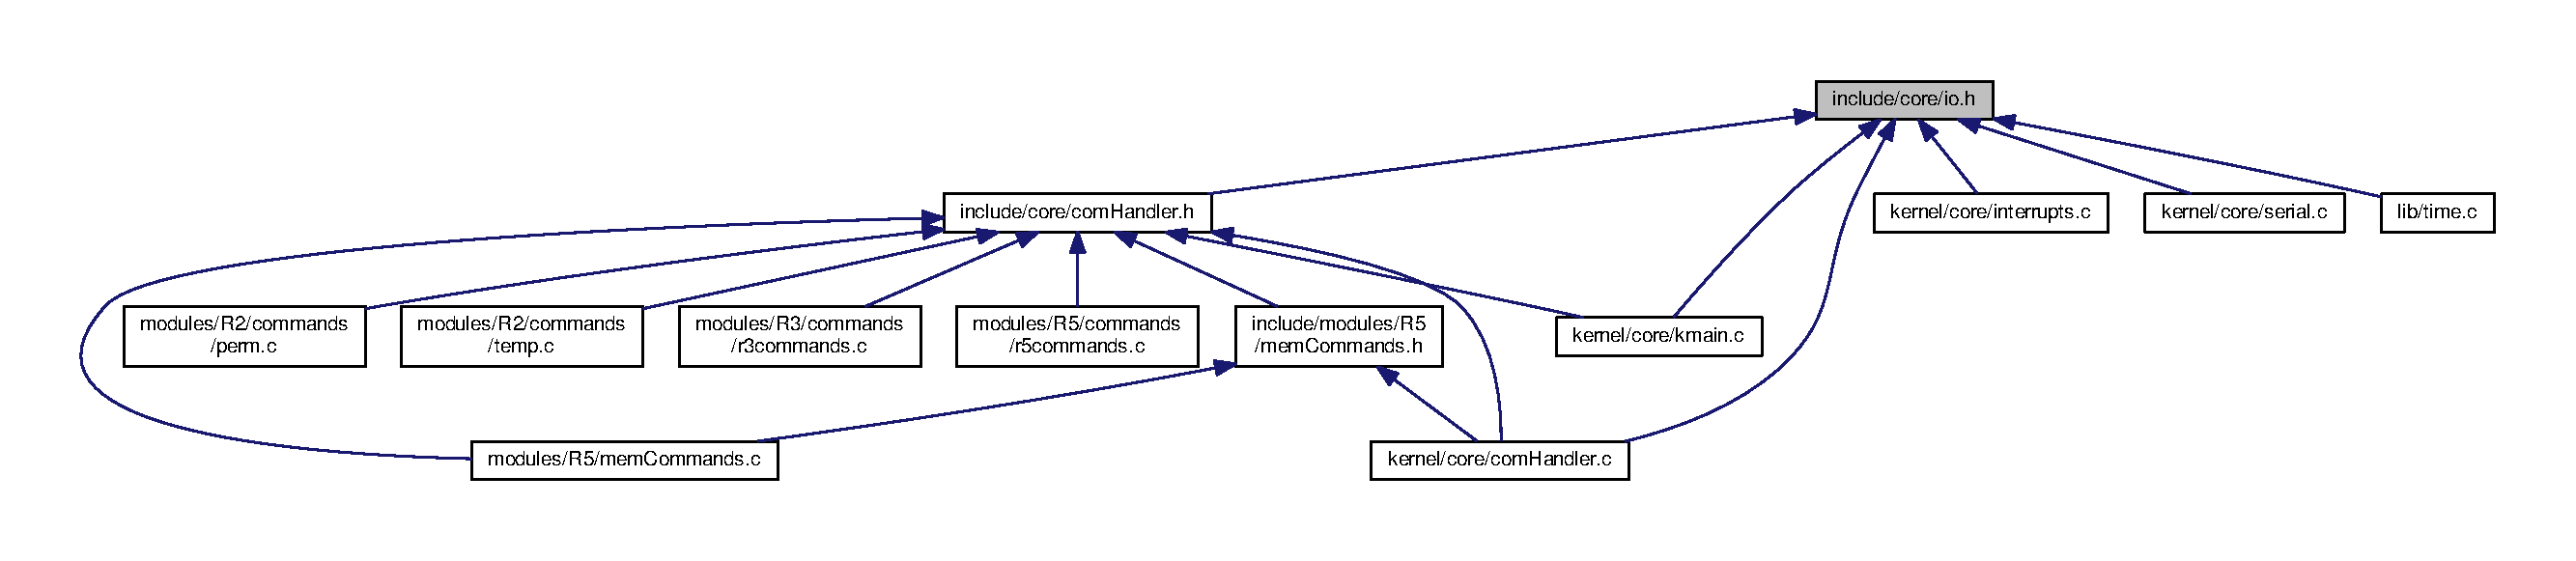
\includegraphics[width=350pt]{io_8h__dep__incl}
\end{center}
\end{figure}
\subsection*{Macros}
\begin{DoxyCompactItemize}
\item 
\#define \hyperlink{io_8h_a0e661d36f40638a36550a534076f155b}{outb}(port,  data)~\hyperlink{system_8h_a71921cebf4610b0dbb2b7a0daaf3fedf}{asm} \hyperlink{system_8h_af55a5e48555be7d32ad73e76cf5d4db0}{volatile} (\char`\"{}outb \%\%al,\%\%dx\char`\"{} \+: \+: \char`\"{}a\char`\"{} (data), \char`\"{}d\char`\"{} (port))
\item 
\#define \hyperlink{io_8h_ad6488a48837d179b1833e2f48dac9665}{inb}(port)
\end{DoxyCompactItemize}


\subsection{Macro Definition Documentation}
\index{io.\+h@{io.\+h}!inb@{inb}}
\index{inb@{inb}!io.\+h@{io.\+h}}
\subsubsection[{\texorpdfstring{inb}{inb}}]{\setlength{\rightskip}{0pt plus 5cm}\#define inb(
\begin{DoxyParamCaption}
\item[{}]{port}
\end{DoxyParamCaption}
)}\hypertarget{io_8h_ad6488a48837d179b1833e2f48dac9665}{}\label{io_8h_ad6488a48837d179b1833e2f48dac9665}
{\bfseries Value\+:}
\begin{DoxyCode}
(\{                                        \(\backslash\)
      unsigned \textcolor{keywordtype}{char} r;                                      \hyperlink{system_8h_a71921cebf4610b0dbb2b7a0daaf3fedf}{\(\backslash\)}
\hyperlink{system_8h_a71921cebf4610b0dbb2b7a0daaf3fedf}{      asm} \textcolor{keyword}{volatile} (\textcolor{stringliteral}{"inb %%dx,%%al"}: \textcolor{stringliteral}{"=a"} (r): \textcolor{stringliteral}{"d"} (port)); \(\backslash\)
      r;                                                    \(\backslash\)
    \})
\end{DoxyCode}
Reads a byte of data from a port.


\begin{DoxyParams}{Parameters}
{\em port} & The port to read the data from \\
\hline
\end{DoxyParams}
\begin{DoxyReturn}{Returns}
The byte from the port 
\end{DoxyReturn}
\index{io.\+h@{io.\+h}!outb@{outb}}
\index{outb@{outb}!io.\+h@{io.\+h}}
\subsubsection[{\texorpdfstring{outb}{outb}}]{\setlength{\rightskip}{0pt plus 5cm}\#define outb(
\begin{DoxyParamCaption}
\item[{}]{port, }
\item[{}]{data}
\end{DoxyParamCaption}
)~{\bf asm} {\bf volatile} (\char`\"{}outb \%\%al,\%\%dx\char`\"{} \+: \+: \char`\"{}a\char`\"{} (data), \char`\"{}d\char`\"{} (port))}\hypertarget{io_8h_a0e661d36f40638a36550a534076f155b}{}\label{io_8h_a0e661d36f40638a36550a534076f155b}
Writes a byte of data to a port.


\begin{DoxyParams}{Parameters}
{\em port} & The port to write the data to \\
\hline
{\em data} & The byte to write \\
\hline
\end{DoxyParams}

\hypertarget{pcb_8h}{}\section{include/core/pcb.h File Reference}
\label{pcb_8h}\index{include/core/pcb.\+h@{include/core/pcb.\+h}}
{\ttfamily \#include $<$system.\+h$>$}\\*
Include dependency graph for pcb.\+h\+:\nopagebreak
\begin{figure}[H]
\begin{center}
\leavevmode
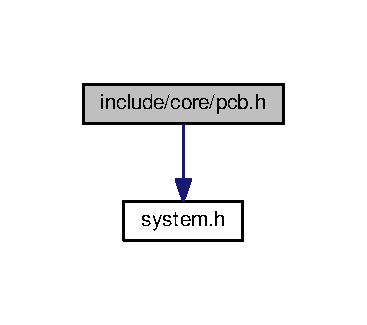
\includegraphics[width=176pt]{pcb_8h__incl}
\end{center}
\end{figure}
This graph shows which files directly or indirectly include this file\+:\nopagebreak
\begin{figure}[H]
\begin{center}
\leavevmode
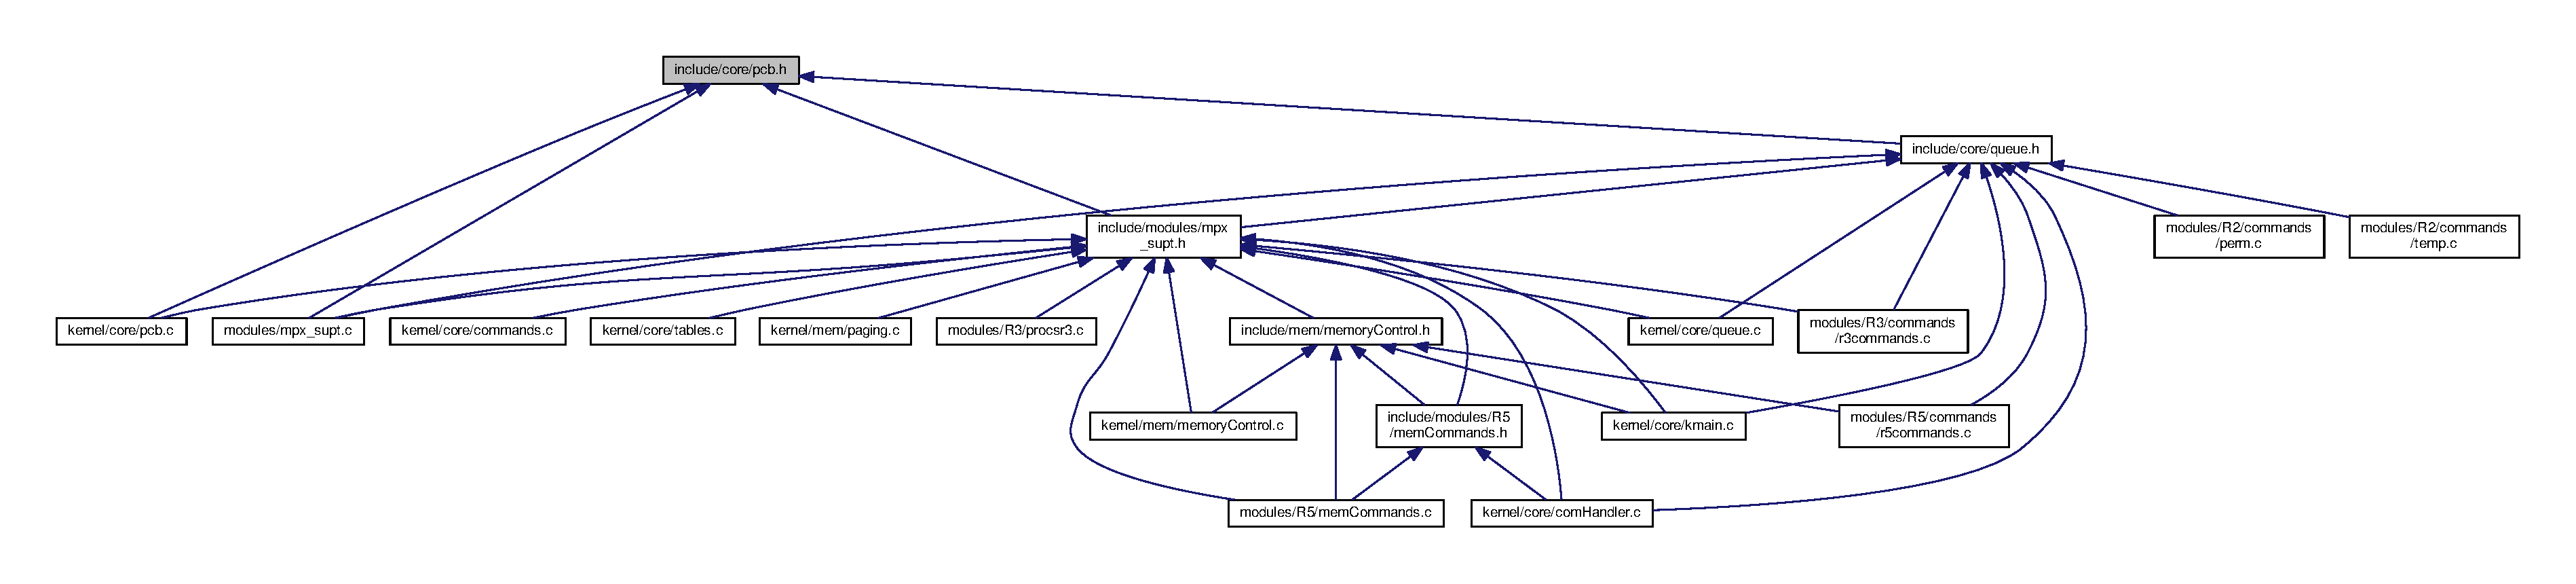
\includegraphics[width=350pt]{pcb_8h__dep__incl}
\end{center}
\end{figure}
\subsection*{Data Structures}
\begin{DoxyCompactItemize}
\item 
struct \hyperlink{structpcb}{pcb}
\end{DoxyCompactItemize}
\subsection*{Macros}
\begin{DoxyCompactItemize}
\item 
\#define \hyperlink{pcb_8h_a48f6457243719e7031768d4100741159}{B\+L\+O\+C\+K\+ED}~0
\item 
\#define \hyperlink{pcb_8h_ad1235d5ce36f7267285e82dccd428aa6}{R\+E\+A\+DY}~1
\item 
\#define \hyperlink{pcb_8h_a6fb7181d994ee98e735494be55809708}{R\+U\+N\+N\+I\+NG}~2
\item 
\#define \hyperlink{pcb_8h_a21b97df85e65556468b28a576311271c}{S\+Y\+S\+T\+EM}~0
\item 
\#define \hyperlink{pcb_8h_a796bd7c6ba2e59281760fb155c6287e8}{A\+P\+P\+L\+I\+C\+A\+T\+I\+ON}~1
\end{DoxyCompactItemize}
\subsection*{Typedefs}
\begin{DoxyCompactItemize}
\item 
typedef struct \hyperlink{structpcb}{pcb} \hyperlink{pcb_8h_a1344afeb2018949c9ac2311b1faea6dc}{pcb}
\end{DoxyCompactItemize}
\subsection*{Functions}
\begin{DoxyCompactItemize}
\item 
\hyperlink{structpcb}{pcb} $\ast$ \hyperlink{pcb_8h_abaf5a209b901d0648067e94079dffe22}{allocate\+P\+CB} ()
\item 
int \hyperlink{pcb_8h_a3cee34bfa271f759a131e81daa5d0072}{free\+P\+CB} (\hyperlink{structpcb}{pcb} $\ast$pcb\+Ptr)
\item 
\hyperlink{structpcb}{pcb} $\ast$ \hyperlink{pcb_8h_a1065e090df16a86b2a477b62e41fa930}{setup\+P\+CB} (const char $\ast$process\+Name, int process\+Class, int priority)
\item 
int \hyperlink{pcb_8h_aaed194f50a1015f4eb373410c81ff23e}{check\+Param\+Name} (const char $\ast$process\+Name)
\item 
int \hyperlink{pcb_8h_ab90a90289554c475abb4f74b71db8163}{check\+Param\+Class} (int process\+Class)
\item 
int \hyperlink{pcb_8h_a0af587ecb3f21b5049b335b62dd44fcf}{check\+Param\+Priority} (int priority)
\end{DoxyCompactItemize}


\subsection{Macro Definition Documentation}
\index{pcb.\+h@{pcb.\+h}!A\+P\+P\+L\+I\+C\+A\+T\+I\+ON@{A\+P\+P\+L\+I\+C\+A\+T\+I\+ON}}
\index{A\+P\+P\+L\+I\+C\+A\+T\+I\+ON@{A\+P\+P\+L\+I\+C\+A\+T\+I\+ON}!pcb.\+h@{pcb.\+h}}
\subsubsection[{\texorpdfstring{A\+P\+P\+L\+I\+C\+A\+T\+I\+ON}{APPLICATION}}]{\setlength{\rightskip}{0pt plus 5cm}\#define A\+P\+P\+L\+I\+C\+A\+T\+I\+ON~1}\hypertarget{pcb_8h_a796bd7c6ba2e59281760fb155c6287e8}{}\label{pcb_8h_a796bd7c6ba2e59281760fb155c6287e8}
\index{pcb.\+h@{pcb.\+h}!B\+L\+O\+C\+K\+ED@{B\+L\+O\+C\+K\+ED}}
\index{B\+L\+O\+C\+K\+ED@{B\+L\+O\+C\+K\+ED}!pcb.\+h@{pcb.\+h}}
\subsubsection[{\texorpdfstring{B\+L\+O\+C\+K\+ED}{BLOCKED}}]{\setlength{\rightskip}{0pt plus 5cm}\#define B\+L\+O\+C\+K\+ED~0}\hypertarget{pcb_8h_a48f6457243719e7031768d4100741159}{}\label{pcb_8h_a48f6457243719e7031768d4100741159}
\index{pcb.\+h@{pcb.\+h}!R\+E\+A\+DY@{R\+E\+A\+DY}}
\index{R\+E\+A\+DY@{R\+E\+A\+DY}!pcb.\+h@{pcb.\+h}}
\subsubsection[{\texorpdfstring{R\+E\+A\+DY}{READY}}]{\setlength{\rightskip}{0pt plus 5cm}\#define R\+E\+A\+DY~1}\hypertarget{pcb_8h_ad1235d5ce36f7267285e82dccd428aa6}{}\label{pcb_8h_ad1235d5ce36f7267285e82dccd428aa6}
\index{pcb.\+h@{pcb.\+h}!R\+U\+N\+N\+I\+NG@{R\+U\+N\+N\+I\+NG}}
\index{R\+U\+N\+N\+I\+NG@{R\+U\+N\+N\+I\+NG}!pcb.\+h@{pcb.\+h}}
\subsubsection[{\texorpdfstring{R\+U\+N\+N\+I\+NG}{RUNNING}}]{\setlength{\rightskip}{0pt plus 5cm}\#define R\+U\+N\+N\+I\+NG~2}\hypertarget{pcb_8h_a6fb7181d994ee98e735494be55809708}{}\label{pcb_8h_a6fb7181d994ee98e735494be55809708}
\index{pcb.\+h@{pcb.\+h}!S\+Y\+S\+T\+EM@{S\+Y\+S\+T\+EM}}
\index{S\+Y\+S\+T\+EM@{S\+Y\+S\+T\+EM}!pcb.\+h@{pcb.\+h}}
\subsubsection[{\texorpdfstring{S\+Y\+S\+T\+EM}{SYSTEM}}]{\setlength{\rightskip}{0pt plus 5cm}\#define S\+Y\+S\+T\+EM~0}\hypertarget{pcb_8h_a21b97df85e65556468b28a576311271c}{}\label{pcb_8h_a21b97df85e65556468b28a576311271c}


\subsection{Typedef Documentation}
\index{pcb.\+h@{pcb.\+h}!pcb@{pcb}}
\index{pcb@{pcb}!pcb.\+h@{pcb.\+h}}
\subsubsection[{\texorpdfstring{pcb}{pcb}}]{\setlength{\rightskip}{0pt plus 5cm}typedef struct {\bf pcb}  {\bf pcb}}\hypertarget{pcb_8h_a1344afeb2018949c9ac2311b1faea6dc}{}\label{pcb_8h_a1344afeb2018949c9ac2311b1faea6dc}


\subsection{Function Documentation}
\index{pcb.\+h@{pcb.\+h}!allocate\+P\+CB@{allocate\+P\+CB}}
\index{allocate\+P\+CB@{allocate\+P\+CB}!pcb.\+h@{pcb.\+h}}
\subsubsection[{\texorpdfstring{allocate\+P\+C\+B()}{allocatePCB()}}]{\setlength{\rightskip}{0pt plus 5cm}{\bf pcb}$\ast$ allocate\+P\+CB (
\begin{DoxyParamCaption}
{}
\end{DoxyParamCaption}
)}\hypertarget{pcb_8h_abaf5a209b901d0648067e94079dffe22}{}\label{pcb_8h_abaf5a209b901d0648067e94079dffe22}
Allocates memory for a new P\+CB and returns a pointer to it

\begin{DoxyReturn}{Returns}
P\+CB pointer or Null if error occurs
\end{DoxyReturn}
Allocates memory for a new P\+CB and returns a pointer to it

free\+P\+CB should be used when done using the pcb to free the memory in use

\begin{DoxyReturn}{Returns}
P\+CB pointer or Null if error occurs 
\end{DoxyReturn}
\index{pcb.\+h@{pcb.\+h}!check\+Param\+Class@{check\+Param\+Class}}
\index{check\+Param\+Class@{check\+Param\+Class}!pcb.\+h@{pcb.\+h}}
\subsubsection[{\texorpdfstring{check\+Param\+Class(int process\+Class)}{checkParamClass(int processClass)}}]{\setlength{\rightskip}{0pt plus 5cm}int check\+Param\+Class (
\begin{DoxyParamCaption}
\item[{int}]{process\+Class}
\end{DoxyParamCaption}
)}\hypertarget{pcb_8h_ab90a90289554c475abb4f74b71db8163}{}\label{pcb_8h_ab90a90289554c475abb4f74b71db8163}
Validates that the process\+Class is valid


\begin{DoxyParams}{Parameters}
{\em process\+Class} & -\/ int \\
\hline
\end{DoxyParams}
\begin{DoxyReturn}{Returns}
integer 0 or 1 if valid 
\end{DoxyReturn}
\index{pcb.\+h@{pcb.\+h}!check\+Param\+Name@{check\+Param\+Name}}
\index{check\+Param\+Name@{check\+Param\+Name}!pcb.\+h@{pcb.\+h}}
\subsubsection[{\texorpdfstring{check\+Param\+Name(const char $\ast$process\+Name)}{checkParamName(const char *processName)}}]{\setlength{\rightskip}{0pt plus 5cm}int check\+Param\+Name (
\begin{DoxyParamCaption}
\item[{const char $\ast$}]{process\+Name}
\end{DoxyParamCaption}
)}\hypertarget{pcb_8h_aaed194f50a1015f4eb373410c81ff23e}{}\label{pcb_8h_aaed194f50a1015f4eb373410c81ff23e}
Validates that the process\+Name is valid


\begin{DoxyParams}{Parameters}
{\em process\+Name} & -\/ const char $\ast$ process\+Name \\
\hline
\end{DoxyParams}
\begin{DoxyReturn}{Returns}
integer 0 or 1 if valid 
\end{DoxyReturn}
\index{pcb.\+h@{pcb.\+h}!check\+Param\+Priority@{check\+Param\+Priority}}
\index{check\+Param\+Priority@{check\+Param\+Priority}!pcb.\+h@{pcb.\+h}}
\subsubsection[{\texorpdfstring{check\+Param\+Priority(int priority)}{checkParamPriority(int priority)}}]{\setlength{\rightskip}{0pt plus 5cm}int check\+Param\+Priority (
\begin{DoxyParamCaption}
\item[{int}]{priority}
\end{DoxyParamCaption}
)}\hypertarget{pcb_8h_a0af587ecb3f21b5049b335b62dd44fcf}{}\label{pcb_8h_a0af587ecb3f21b5049b335b62dd44fcf}
Validates that the priority is valid


\begin{DoxyParams}{Parameters}
{\em priority} & -\/ int \\
\hline
\end{DoxyParams}
\begin{DoxyReturn}{Returns}
integer 0 or 1 if valid 
\end{DoxyReturn}
\index{pcb.\+h@{pcb.\+h}!free\+P\+CB@{free\+P\+CB}}
\index{free\+P\+CB@{free\+P\+CB}!pcb.\+h@{pcb.\+h}}
\subsubsection[{\texorpdfstring{free\+P\+C\+B(pcb $\ast$pcb\+Ptr)}{freePCB(pcb *pcbPtr)}}]{\setlength{\rightskip}{0pt plus 5cm}int free\+P\+CB (
\begin{DoxyParamCaption}
\item[{{\bf pcb} $\ast$}]{pcb\+Ptr}
\end{DoxyParamCaption}
)}\hypertarget{pcb_8h_a3cee34bfa271f759a131e81daa5d0072}{}\label{pcb_8h_a3cee34bfa271f759a131e81daa5d0072}
Frees memory that is allocated for the pcb provided


\begin{DoxyParams}{Parameters}
{\em pcb\+Ptr} & pointer to pcb to be freed \\
\hline
\end{DoxyParams}
\begin{DoxyReturn}{Returns}
integer code -\/ 1 if successful, -\/1 otherwise
\end{DoxyReturn}
Frees memory that is allocated for the pcb provided


\begin{DoxyParams}{Parameters}
{\em pcb\+Ptr} & pointer to pcb to be freed \\
\hline
\end{DoxyParams}
\begin{DoxyReturn}{Returns}
integer code -\/ 1 if successful, 0 otherwise 
\end{DoxyReturn}
\index{pcb.\+h@{pcb.\+h}!setup\+P\+CB@{setup\+P\+CB}}
\index{setup\+P\+CB@{setup\+P\+CB}!pcb.\+h@{pcb.\+h}}
\subsubsection[{\texorpdfstring{setup\+P\+C\+B(const char $\ast$process\+Name, int process\+Class, int priority)}{setupPCB(const char *processName, int processClass, int priority)}}]{\setlength{\rightskip}{0pt plus 5cm}{\bf pcb}$\ast$ setup\+P\+CB (
\begin{DoxyParamCaption}
\item[{const char $\ast$}]{process\+Name, }
\item[{int}]{process\+Class, }
\item[{int}]{priority}
\end{DoxyParamCaption}
)}\hypertarget{pcb_8h_a1065e090df16a86b2a477b62e41fa930}{}\label{pcb_8h_a1065e090df16a86b2a477b62e41fa930}
Allocates memory for a new P\+CB and sets it with given params


\begin{DoxyParams}{Parameters}
{\em process\+Name} & -\/ const string name \\
\hline
{\em process\+Class} & -\/ integer identifying as system or application process (0, 1) \\
\hline
{\em priority} & -\/ integer between 0 and 9 indicating priority \\
\hline
\end{DoxyParams}
\begin{DoxyReturn}{Returns}
P\+CB pointer to new pcb or N\+U\+LL if there were errors 
\end{DoxyReturn}

\hypertarget{queue_8h}{}\section{include/core/queue.h File Reference}
\label{queue_8h}\index{include/core/queue.\+h@{include/core/queue.\+h}}
{\ttfamily \#include \char`\"{}pcb.\+h\char`\"{}}\\*
{\ttfamily \#include \char`\"{}boolean.\+h\char`\"{}}\\*
Include dependency graph for queue.\+h\+:\nopagebreak
\begin{figure}[H]
\begin{center}
\leavevmode
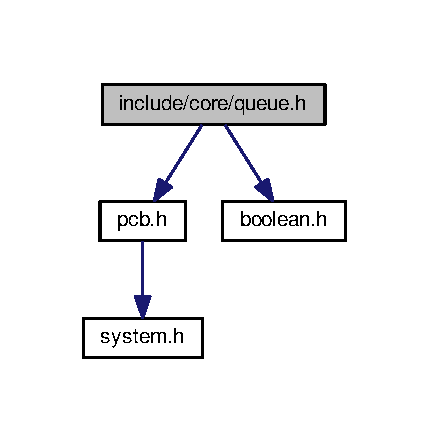
\includegraphics[width=206pt]{queue_8h__incl}
\end{center}
\end{figure}
This graph shows which files directly or indirectly include this file\+:\nopagebreak
\begin{figure}[H]
\begin{center}
\leavevmode
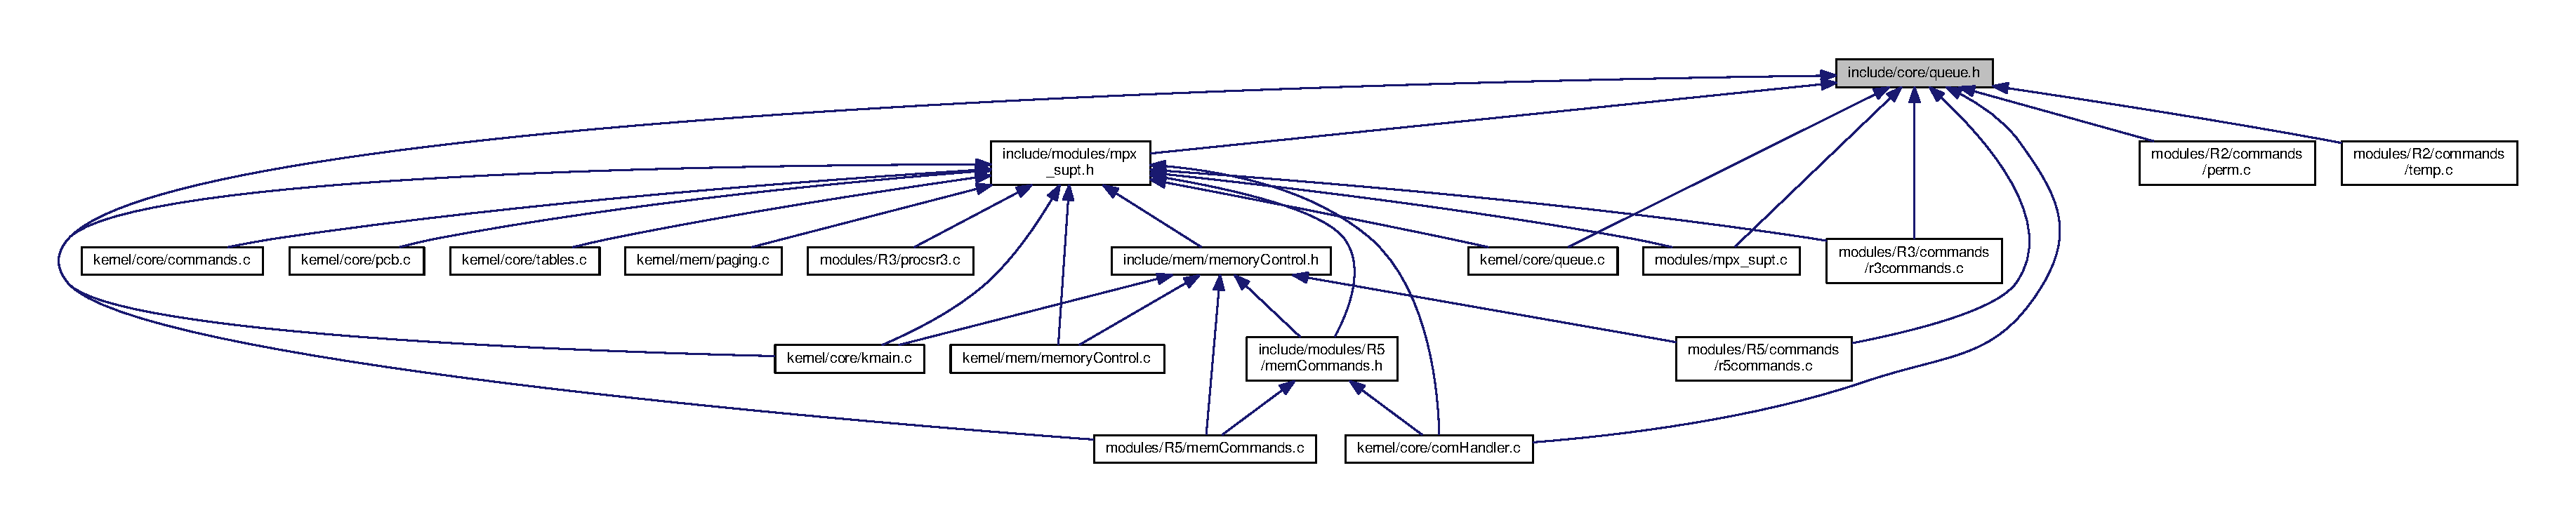
\includegraphics[width=350pt]{queue_8h__dep__incl}
\end{center}
\end{figure}
\subsection*{Data Structures}
\begin{DoxyCompactItemize}
\item 
struct \hyperlink{structnode}{node}
\end{DoxyCompactItemize}
\subsection*{Typedefs}
\begin{DoxyCompactItemize}
\item 
typedef struct \hyperlink{structnode}{node} \hyperlink{queue_8h_ace29f146c273d2654669dc2c710603e2}{node}
\end{DoxyCompactItemize}
\subsection*{Functions}
\begin{DoxyCompactItemize}
\item 
\hyperlink{structnode}{node} $\ast$ \hyperlink{queue_8h_a90ecf077bdf2731051966c1fc72f619b}{get\+Ready\+Queue} ()
\item 
\hyperlink{structnode}{node} $\ast$ \hyperlink{queue_8h_a5170ee107f4bc7e352d4407395d57da7}{get\+Blocked\+Queue} ()
\item 
\hyperlink{structnode}{node} $\ast$ \hyperlink{queue_8h_a10529b60bfa07efe56794a575af1721d}{get\+Suspended\+Ready\+Queue} ()
\item 
\hyperlink{structnode}{node} $\ast$ \hyperlink{queue_8h_a9f027fce172315eed8a8893192af6421}{get\+Suspended\+Blocked\+Queue} ()
\item 
\hyperlink{structpcb}{pcb} $\ast$ \hyperlink{queue_8h_a9d45db295536fc5e43d7ba34b1984157}{pop\+Ready} ()
\item 
\hyperlink{structpcb}{pcb} $\ast$ \hyperlink{queue_8h_a349201cc823df4797c37a24bf34d2014}{pop\+Blocked} ()
\item 
\hyperlink{structpcb}{pcb} $\ast$ \hyperlink{queue_8h_a2986335d1a7e14f5b65173253a911882}{pop\+Suspended\+Ready} ()
\item 
\hyperlink{structpcb}{pcb} $\ast$ \hyperlink{queue_8h_a1a011f09bcd31aa910535aba088ab537}{pop\+Suspended\+Blocked} ()
\item 
\hyperlink{boolean_8h_a7c6368b321bd9acd0149b030bb8275ed}{boolean} \hyperlink{queue_8h_a7d2249981425ab391895a81820d3f221}{insert\+P\+CB} (\hyperlink{structpcb}{pcb} $\ast$p)
\item 
\hyperlink{boolean_8h_a7c6368b321bd9acd0149b030bb8275ed}{boolean} \hyperlink{queue_8h_a305ebe6c5f7cdd7731706cae59d43e33}{remove\+P\+CB} (\hyperlink{structpcb}{pcb} $\ast$p)
\item 
\hyperlink{structpcb}{pcb} $\ast$ \hyperlink{queue_8h_a291648ddfe62eec41c502cee840c98da}{find\+P\+CB} (const char $\ast$process\+Name)
\end{DoxyCompactItemize}


\subsection{Typedef Documentation}
\index{queue.\+h@{queue.\+h}!node@{node}}
\index{node@{node}!queue.\+h@{queue.\+h}}
\subsubsection[{\texorpdfstring{node}{node}}]{\setlength{\rightskip}{0pt plus 5cm}typedef struct {\bf node}  {\bf node}}\hypertarget{queue_8h_ace29f146c273d2654669dc2c710603e2}{}\label{queue_8h_ace29f146c273d2654669dc2c710603e2}
The struct representing a node in a queue 

\subsection{Function Documentation}
\index{queue.\+h@{queue.\+h}!find\+P\+CB@{find\+P\+CB}}
\index{find\+P\+CB@{find\+P\+CB}!queue.\+h@{queue.\+h}}
\subsubsection[{\texorpdfstring{find\+P\+C\+B(const char $\ast$process\+Name)}{findPCB(const char *processName)}}]{\setlength{\rightskip}{0pt plus 5cm}{\bf pcb}$\ast$ find\+P\+CB (
\begin{DoxyParamCaption}
\item[{const char $\ast$}]{process\+Name}
\end{DoxyParamCaption}
)}\hypertarget{queue_8h_a291648ddfe62eec41c502cee840c98da}{}\label{queue_8h_a291648ddfe62eec41c502cee840c98da}
Finds the P\+CB with the given process name.


\begin{DoxyParams}{Parameters}
{\em process\+Name} & The name of the process to search for \\
\hline
\end{DoxyParams}
\begin{DoxyReturn}{Returns}
A pointer to the P\+CB, or null if not found 
\end{DoxyReturn}
\index{queue.\+h@{queue.\+h}!get\+Blocked\+Queue@{get\+Blocked\+Queue}}
\index{get\+Blocked\+Queue@{get\+Blocked\+Queue}!queue.\+h@{queue.\+h}}
\subsubsection[{\texorpdfstring{get\+Blocked\+Queue()}{getBlockedQueue()}}]{\setlength{\rightskip}{0pt plus 5cm}{\bf node}$\ast$ get\+Blocked\+Queue (
\begin{DoxyParamCaption}
{}
\end{DoxyParamCaption}
)}\hypertarget{queue_8h_a5170ee107f4bc7e352d4407395d57da7}{}\label{queue_8h_a5170ee107f4bc7e352d4407395d57da7}
Gets the head node of the blocked queue.

\begin{DoxyReturn}{Returns}
The head node of the blocked queue 
\end{DoxyReturn}
\index{queue.\+h@{queue.\+h}!get\+Ready\+Queue@{get\+Ready\+Queue}}
\index{get\+Ready\+Queue@{get\+Ready\+Queue}!queue.\+h@{queue.\+h}}
\subsubsection[{\texorpdfstring{get\+Ready\+Queue()}{getReadyQueue()}}]{\setlength{\rightskip}{0pt plus 5cm}{\bf node}$\ast$ get\+Ready\+Queue (
\begin{DoxyParamCaption}
{}
\end{DoxyParamCaption}
)}\hypertarget{queue_8h_a90ecf077bdf2731051966c1fc72f619b}{}\label{queue_8h_a90ecf077bdf2731051966c1fc72f619b}
Gets the head node of the ready queue.

\begin{DoxyReturn}{Returns}
The head node of the ready queue 
\end{DoxyReturn}
\index{queue.\+h@{queue.\+h}!get\+Suspended\+Blocked\+Queue@{get\+Suspended\+Blocked\+Queue}}
\index{get\+Suspended\+Blocked\+Queue@{get\+Suspended\+Blocked\+Queue}!queue.\+h@{queue.\+h}}
\subsubsection[{\texorpdfstring{get\+Suspended\+Blocked\+Queue()}{getSuspendedBlockedQueue()}}]{\setlength{\rightskip}{0pt plus 5cm}{\bf node}$\ast$ get\+Suspended\+Blocked\+Queue (
\begin{DoxyParamCaption}
{}
\end{DoxyParamCaption}
)}\hypertarget{queue_8h_a9f027fce172315eed8a8893192af6421}{}\label{queue_8h_a9f027fce172315eed8a8893192af6421}
Gets the head node of the suspended-\/blocked queue.

\begin{DoxyReturn}{Returns}
The head node of the suspended-\/blocked queue 
\end{DoxyReturn}
\index{queue.\+h@{queue.\+h}!get\+Suspended\+Ready\+Queue@{get\+Suspended\+Ready\+Queue}}
\index{get\+Suspended\+Ready\+Queue@{get\+Suspended\+Ready\+Queue}!queue.\+h@{queue.\+h}}
\subsubsection[{\texorpdfstring{get\+Suspended\+Ready\+Queue()}{getSuspendedReadyQueue()}}]{\setlength{\rightskip}{0pt plus 5cm}{\bf node}$\ast$ get\+Suspended\+Ready\+Queue (
\begin{DoxyParamCaption}
{}
\end{DoxyParamCaption}
)}\hypertarget{queue_8h_a10529b60bfa07efe56794a575af1721d}{}\label{queue_8h_a10529b60bfa07efe56794a575af1721d}
Gets the head node of the suspended-\/ready queue.

\begin{DoxyReturn}{Returns}
The head node of the suspended-\/ready queue 
\end{DoxyReturn}
\index{queue.\+h@{queue.\+h}!insert\+P\+CB@{insert\+P\+CB}}
\index{insert\+P\+CB@{insert\+P\+CB}!queue.\+h@{queue.\+h}}
\subsubsection[{\texorpdfstring{insert\+P\+C\+B(pcb $\ast$p)}{insertPCB(pcb *p)}}]{\setlength{\rightskip}{0pt plus 5cm}{\bf boolean} insert\+P\+CB (
\begin{DoxyParamCaption}
\item[{{\bf pcb} $\ast$}]{p}
\end{DoxyParamCaption}
)}\hypertarget{queue_8h_a7d2249981425ab391895a81820d3f221}{}\label{queue_8h_a7d2249981425ab391895a81820d3f221}
Inserts the P\+CB into the appropriate queue.


\begin{DoxyParams}{Parameters}
{\em p} & The P\+CB to insert. \\
\hline
\end{DoxyParams}
\begin{DoxyReturn}{Returns}
true if the P\+CB was inserted, false otherwise 
\end{DoxyReturn}
\index{queue.\+h@{queue.\+h}!pop\+Blocked@{pop\+Blocked}}
\index{pop\+Blocked@{pop\+Blocked}!queue.\+h@{queue.\+h}}
\subsubsection[{\texorpdfstring{pop\+Blocked()}{popBlocked()}}]{\setlength{\rightskip}{0pt plus 5cm}{\bf pcb}$\ast$ pop\+Blocked (
\begin{DoxyParamCaption}
{}
\end{DoxyParamCaption}
)}\hypertarget{queue_8h_a349201cc823df4797c37a24bf34d2014}{}\label{queue_8h_a349201cc823df4797c37a24bf34d2014}
Pops the next node off of the blocked queue.

\begin{DoxyReturn}{Returns}
The next node of the blocked queue, or N\+U\+LL if it is empty 
\end{DoxyReturn}
\index{queue.\+h@{queue.\+h}!pop\+Ready@{pop\+Ready}}
\index{pop\+Ready@{pop\+Ready}!queue.\+h@{queue.\+h}}
\subsubsection[{\texorpdfstring{pop\+Ready()}{popReady()}}]{\setlength{\rightskip}{0pt plus 5cm}{\bf pcb}$\ast$ pop\+Ready (
\begin{DoxyParamCaption}
{}
\end{DoxyParamCaption}
)}\hypertarget{queue_8h_a9d45db295536fc5e43d7ba34b1984157}{}\label{queue_8h_a9d45db295536fc5e43d7ba34b1984157}
Pops the next node off of the ready queue.

\begin{DoxyReturn}{Returns}
The next node of the ready queue, or N\+U\+LL if it is empty 
\end{DoxyReturn}
\index{queue.\+h@{queue.\+h}!pop\+Suspended\+Blocked@{pop\+Suspended\+Blocked}}
\index{pop\+Suspended\+Blocked@{pop\+Suspended\+Blocked}!queue.\+h@{queue.\+h}}
\subsubsection[{\texorpdfstring{pop\+Suspended\+Blocked()}{popSuspendedBlocked()}}]{\setlength{\rightskip}{0pt plus 5cm}{\bf pcb}$\ast$ pop\+Suspended\+Blocked (
\begin{DoxyParamCaption}
{}
\end{DoxyParamCaption}
)}\hypertarget{queue_8h_a1a011f09bcd31aa910535aba088ab537}{}\label{queue_8h_a1a011f09bcd31aa910535aba088ab537}
Pops the next node off of the suspended-\/blocked queue.

\begin{DoxyReturn}{Returns}
The next node of the suspended-\/blocked queue, or N\+U\+LL if it is empty 
\end{DoxyReturn}
\index{queue.\+h@{queue.\+h}!pop\+Suspended\+Ready@{pop\+Suspended\+Ready}}
\index{pop\+Suspended\+Ready@{pop\+Suspended\+Ready}!queue.\+h@{queue.\+h}}
\subsubsection[{\texorpdfstring{pop\+Suspended\+Ready()}{popSuspendedReady()}}]{\setlength{\rightskip}{0pt plus 5cm}{\bf pcb}$\ast$ pop\+Suspended\+Ready (
\begin{DoxyParamCaption}
{}
\end{DoxyParamCaption}
)}\hypertarget{queue_8h_a2986335d1a7e14f5b65173253a911882}{}\label{queue_8h_a2986335d1a7e14f5b65173253a911882}
Pops the next node off of the suspended-\/ready queue.

\begin{DoxyReturn}{Returns}
The next node of the suspended-\/ready queue, or N\+U\+LL if it is empty 
\end{DoxyReturn}
\index{queue.\+h@{queue.\+h}!remove\+P\+CB@{remove\+P\+CB}}
\index{remove\+P\+CB@{remove\+P\+CB}!queue.\+h@{queue.\+h}}
\subsubsection[{\texorpdfstring{remove\+P\+C\+B(pcb $\ast$p)}{removePCB(pcb *p)}}]{\setlength{\rightskip}{0pt plus 5cm}{\bf boolean} remove\+P\+CB (
\begin{DoxyParamCaption}
\item[{{\bf pcb} $\ast$}]{p}
\end{DoxyParamCaption}
)}\hypertarget{queue_8h_a305ebe6c5f7cdd7731706cae59d43e33}{}\label{queue_8h_a305ebe6c5f7cdd7731706cae59d43e33}
Removes the given P\+CB from it\textquotesingle{}s queue.


\begin{DoxyParams}{Parameters}
{\em p} & The P\+CB to remove \\
\hline
\end{DoxyParams}
\begin{DoxyReturn}{Returns}
true if the P\+CB was removed, false otherwise 
\end{DoxyReturn}

\hypertarget{serial_8h}{}\section{include/core/serial.h File Reference}
\label{serial_8h}\index{include/core/serial.\+h@{include/core/serial.\+h}}
This graph shows which files directly or indirectly include this file\+:\nopagebreak
\begin{figure}[H]
\begin{center}
\leavevmode
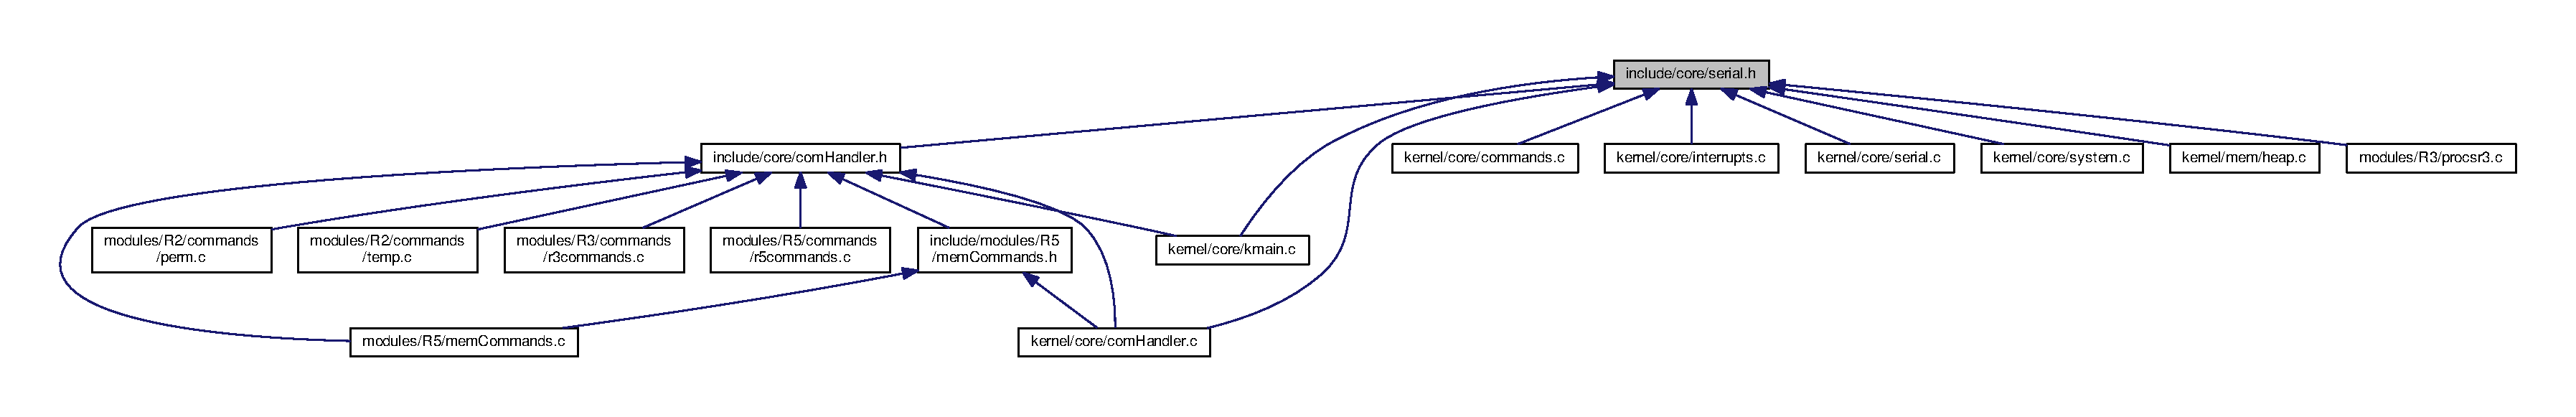
\includegraphics[width=350pt]{serial_8h__dep__incl}
\end{center}
\end{figure}
\subsection*{Macros}
\begin{DoxyCompactItemize}
\item 
\#define \hyperlink{serial_8h_a00dbb3ab1c59e14699be9393693e2248}{C\+O\+M1}~0x3f8
\item 
\#define \hyperlink{serial_8h_a435e02f194c24c9b0e00d7cd27a1704e}{C\+O\+M2}~0x2f8
\item 
\#define \hyperlink{serial_8h_abbed02672431595364c5dd35809303a6}{C\+O\+M3}~0x3e8
\item 
\#define \hyperlink{serial_8h_a595cabb01568ba641574d24546d99c6b}{C\+O\+M4}~0x2e8
\end{DoxyCompactItemize}
\subsection*{Functions}
\begin{DoxyCompactItemize}
\item 
int \hyperlink{serial_8h_a7078c07ff8b2c48780558549a8f7cf90}{init\+\_\+serial} (int device)
\item 
int \hyperlink{serial_8h_a3514f7abff236a4e00a6c46021ce5e22}{serial\+\_\+println} (const char $\ast$msg)
\item 
int \hyperlink{serial_8h_a995827efcd4dcfb780c9fbb9645410a4}{serial\+\_\+print} (const char $\ast$msg)
\item 
int \hyperlink{serial_8h_ae97b87ee1f57c687e7fca6f9958e03ef}{set\+\_\+serial\+\_\+out} (int device)
\item 
int \hyperlink{serial_8h_a3f4008da5feabfb7e086f6673a81104b}{set\+\_\+serial\+\_\+in} (int device)
\end{DoxyCompactItemize}


\subsection{Macro Definition Documentation}
\index{serial.\+h@{serial.\+h}!C\+O\+M1@{C\+O\+M1}}
\index{C\+O\+M1@{C\+O\+M1}!serial.\+h@{serial.\+h}}
\subsubsection[{\texorpdfstring{C\+O\+M1}{COM1}}]{\setlength{\rightskip}{0pt plus 5cm}\#define C\+O\+M1~0x3f8}\hypertarget{serial_8h_a00dbb3ab1c59e14699be9393693e2248}{}\label{serial_8h_a00dbb3ab1c59e14699be9393693e2248}
\index{serial.\+h@{serial.\+h}!C\+O\+M2@{C\+O\+M2}}
\index{C\+O\+M2@{C\+O\+M2}!serial.\+h@{serial.\+h}}
\subsubsection[{\texorpdfstring{C\+O\+M2}{COM2}}]{\setlength{\rightskip}{0pt plus 5cm}\#define C\+O\+M2~0x2f8}\hypertarget{serial_8h_a435e02f194c24c9b0e00d7cd27a1704e}{}\label{serial_8h_a435e02f194c24c9b0e00d7cd27a1704e}
\index{serial.\+h@{serial.\+h}!C\+O\+M3@{C\+O\+M3}}
\index{C\+O\+M3@{C\+O\+M3}!serial.\+h@{serial.\+h}}
\subsubsection[{\texorpdfstring{C\+O\+M3}{COM3}}]{\setlength{\rightskip}{0pt plus 5cm}\#define C\+O\+M3~0x3e8}\hypertarget{serial_8h_abbed02672431595364c5dd35809303a6}{}\label{serial_8h_abbed02672431595364c5dd35809303a6}
\index{serial.\+h@{serial.\+h}!C\+O\+M4@{C\+O\+M4}}
\index{C\+O\+M4@{C\+O\+M4}!serial.\+h@{serial.\+h}}
\subsubsection[{\texorpdfstring{C\+O\+M4}{COM4}}]{\setlength{\rightskip}{0pt plus 5cm}\#define C\+O\+M4~0x2e8}\hypertarget{serial_8h_a595cabb01568ba641574d24546d99c6b}{}\label{serial_8h_a595cabb01568ba641574d24546d99c6b}


\subsection{Function Documentation}
\index{serial.\+h@{serial.\+h}!init\+\_\+serial@{init\+\_\+serial}}
\index{init\+\_\+serial@{init\+\_\+serial}!serial.\+h@{serial.\+h}}
\subsubsection[{\texorpdfstring{init\+\_\+serial(int device)}{init_serial(int device)}}]{\setlength{\rightskip}{0pt plus 5cm}int init\+\_\+serial (
\begin{DoxyParamCaption}
\item[{int}]{device}
\end{DoxyParamCaption}
)}\hypertarget{serial_8h_a7078c07ff8b2c48780558549a8f7cf90}{}\label{serial_8h_a7078c07ff8b2c48780558549a8f7cf90}
Initializes devices for user interaction, logging, ...


\begin{DoxyParams}{Parameters}
{\em device} & The device to initialize \\
\hline
\end{DoxyParams}
\begin{DoxyReturn}{Returns}
The error code 
\end{DoxyReturn}
\index{serial.\+h@{serial.\+h}!serial\+\_\+print@{serial\+\_\+print}}
\index{serial\+\_\+print@{serial\+\_\+print}!serial.\+h@{serial.\+h}}
\subsubsection[{\texorpdfstring{serial\+\_\+print(const char $\ast$msg)}{serial_print(const char *msg)}}]{\setlength{\rightskip}{0pt plus 5cm}int serial\+\_\+print (
\begin{DoxyParamCaption}
\item[{const char $\ast$}]{msg}
\end{DoxyParamCaption}
)}\hypertarget{serial_8h_a995827efcd4dcfb780c9fbb9645410a4}{}\label{serial_8h_a995827efcd4dcfb780c9fbb9645410a4}
Writes a message to the active serial output device.


\begin{DoxyParams}{Parameters}
{\em msg} & The message to write \\
\hline
\end{DoxyParams}
\begin{DoxyReturn}{Returns}
The error code 
\end{DoxyReturn}
\index{serial.\+h@{serial.\+h}!serial\+\_\+println@{serial\+\_\+println}}
\index{serial\+\_\+println@{serial\+\_\+println}!serial.\+h@{serial.\+h}}
\subsubsection[{\texorpdfstring{serial\+\_\+println(const char $\ast$msg)}{serial_println(const char *msg)}}]{\setlength{\rightskip}{0pt plus 5cm}int serial\+\_\+println (
\begin{DoxyParamCaption}
\item[{const char $\ast$}]{msg}
\end{DoxyParamCaption}
)}\hypertarget{serial_8h_a3514f7abff236a4e00a6c46021ce5e22}{}\label{serial_8h_a3514f7abff236a4e00a6c46021ce5e22}
Writes a message to the active serial output device. Appends a newline character.


\begin{DoxyParams}{Parameters}
{\em msg} & The message to write \\
\hline
\end{DoxyParams}
\begin{DoxyReturn}{Returns}
The error code 
\end{DoxyReturn}
\index{serial.\+h@{serial.\+h}!set\+\_\+serial\+\_\+in@{set\+\_\+serial\+\_\+in}}
\index{set\+\_\+serial\+\_\+in@{set\+\_\+serial\+\_\+in}!serial.\+h@{serial.\+h}}
\subsubsection[{\texorpdfstring{set\+\_\+serial\+\_\+in(int device)}{set_serial_in(int device)}}]{\setlength{\rightskip}{0pt plus 5cm}int set\+\_\+serial\+\_\+in (
\begin{DoxyParamCaption}
\item[{int}]{device}
\end{DoxyParamCaption}
)}\hypertarget{serial_8h_a3f4008da5feabfb7e086f6673a81104b}{}\label{serial_8h_a3f4008da5feabfb7e086f6673a81104b}
Sets serial\+\_\+port\+\_\+in to the given device address. All serial input, such as console input via a virutal machine, Q\+E\+M\+U/\+Bochc/etc, will be directed to the device.


\begin{DoxyParams}{Parameters}
{\em device} & The divce to set as input \\
\hline
\end{DoxyParams}
\begin{DoxyReturn}{Returns}
The error code 
\end{DoxyReturn}
\index{serial.\+h@{serial.\+h}!set\+\_\+serial\+\_\+out@{set\+\_\+serial\+\_\+out}}
\index{set\+\_\+serial\+\_\+out@{set\+\_\+serial\+\_\+out}!serial.\+h@{serial.\+h}}
\subsubsection[{\texorpdfstring{set\+\_\+serial\+\_\+out(int device)}{set_serial_out(int device)}}]{\setlength{\rightskip}{0pt plus 5cm}int set\+\_\+serial\+\_\+out (
\begin{DoxyParamCaption}
\item[{int}]{device}
\end{DoxyParamCaption}
)}\hypertarget{serial_8h_ae97b87ee1f57c687e7fca6f9958e03ef}{}\label{serial_8h_ae97b87ee1f57c687e7fca6f9958e03ef}
Sets serial\+\_\+port\+\_\+out to the given device address. All serial output, such as that from serial\+\_\+println, will be directed to this device.


\begin{DoxyParams}{Parameters}
{\em device} & The device to set as output \\
\hline
\end{DoxyParams}
\begin{DoxyReturn}{Returns}
The error code 
\end{DoxyReturn}

\hypertarget{tables_8h}{}\section{include/core/tables.h File Reference}
\label{tables_8h}\index{include/core/tables.\+h@{include/core/tables.\+h}}
{\ttfamily \#include \char`\"{}system.\+h\char`\"{}}\\*
Include dependency graph for tables.\+h\+:\nopagebreak
\begin{figure}[H]
\begin{center}
\leavevmode
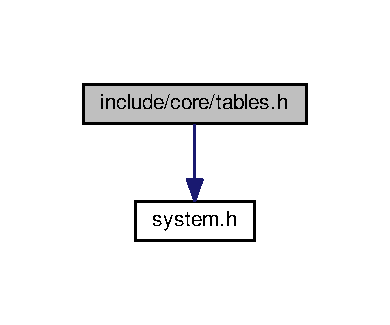
\includegraphics[width=187pt]{tables_8h__incl}
\end{center}
\end{figure}
This graph shows which files directly or indirectly include this file\+:\nopagebreak
\begin{figure}[H]
\begin{center}
\leavevmode
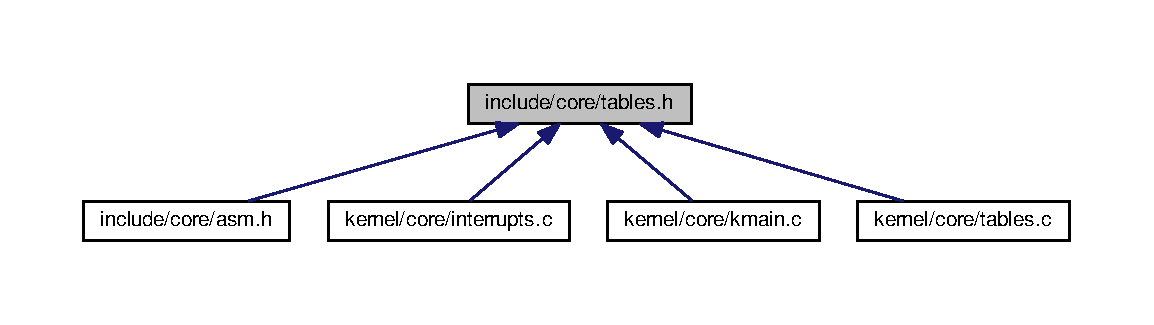
\includegraphics[width=350pt]{tables_8h__dep__incl}
\end{center}
\end{figure}
\subsection*{Data Structures}
\begin{DoxyCompactItemize}
\item 
struct \hyperlink{structidt__entry__struct}{idt\+\_\+entry\+\_\+struct}
\item 
struct \hyperlink{structidt__struct}{idt\+\_\+struct}
\item 
struct \hyperlink{structgdt__descriptor__struct}{gdt\+\_\+descriptor\+\_\+struct}
\item 
struct \hyperlink{structgdt__entry__struct}{gdt\+\_\+entry\+\_\+struct}
\end{DoxyCompactItemize}
\subsection*{Functions}
\begin{DoxyCompactItemize}
\item 
struct \hyperlink{structidt__entry__struct}{idt\+\_\+entry\+\_\+struct} \hyperlink{tables_8h_ad1929ba5e546bde910d88a7c08dc507b}{\+\_\+\+\_\+attribute\+\_\+\+\_\+} ((packed)) idt\+\_\+entry
\item 
void \hyperlink{tables_8h_a9eca3fe1465f8d7d383551d804853139}{idt\+\_\+set\+\_\+gate} (\hyperlink{system_8h_a1026e682ffdadc1701c42cd44ce9efcf}{u8int} idx, \hyperlink{system_8h_a757de76cafbcddaac0d1632902fe4cb8}{u32int} \hyperlink{tables_8h_ab5763c2b18c825c8b8fba44b2e60ddc1}{base}, \hyperlink{system_8h_a863d9497073aad2b991aeab2211d87af}{u16int} sel, \hyperlink{system_8h_a1026e682ffdadc1701c42cd44ce9efcf}{u8int} \hyperlink{tables_8h_a138dda98fcd4738346af61bcca8cf4b4}{flags})
\item 
void \hyperlink{tables_8h_a0b5aee548c88c40ecb07741be1be2e27}{gdt\+\_\+init\+\_\+entry} (int idx, \hyperlink{system_8h_a757de76cafbcddaac0d1632902fe4cb8}{u32int} \hyperlink{tables_8h_ab5763c2b18c825c8b8fba44b2e60ddc1}{base}, \hyperlink{system_8h_a757de76cafbcddaac0d1632902fe4cb8}{u32int} \hyperlink{tables_8h_a68fd3b4f6c14a331ca9b226cbf122e13}{limit}, \hyperlink{system_8h_a1026e682ffdadc1701c42cd44ce9efcf}{u8int} \hyperlink{tables_8h_a360a726ac0b61d9e4e1be3ad34f80244}{access}, \hyperlink{system_8h_a1026e682ffdadc1701c42cd44ce9efcf}{u8int} \hyperlink{tables_8h_a138dda98fcd4738346af61bcca8cf4b4}{flags})
\item 
void \hyperlink{tables_8h_a35fe413107af682030ab7a4b6dff19b8}{init\+\_\+idt} ()
\item 
void \hyperlink{tables_8h_a86bb50044169930202cc403376ef40c3}{init\+\_\+gdt} ()
\end{DoxyCompactItemize}
\subsection*{Variables}
\begin{DoxyCompactItemize}
\item 
\hyperlink{system_8h_a863d9497073aad2b991aeab2211d87af}{u16int} \hyperlink{tables_8h_a0a776dced2c26f16298425cde39f8364}{base\+\_\+low}
\item 
\hyperlink{system_8h_a863d9497073aad2b991aeab2211d87af}{u16int} \hyperlink{tables_8h_ab3f34507900160b4a9b309b4ed039e07}{sselect}
\item 
\hyperlink{system_8h_a1026e682ffdadc1701c42cd44ce9efcf}{u8int} \hyperlink{tables_8h_a94515e42687e7508877c09da81f86860}{zero}
\item 
\hyperlink{system_8h_a1026e682ffdadc1701c42cd44ce9efcf}{u8int} \hyperlink{tables_8h_a138dda98fcd4738346af61bcca8cf4b4}{flags}
\item 
\hyperlink{system_8h_a863d9497073aad2b991aeab2211d87af}{u16int} \hyperlink{tables_8h_a706c81b840522a69ab6e6e941630d5e4}{base\+\_\+high}
\item 
\hyperlink{system_8h_a863d9497073aad2b991aeab2211d87af}{u16int} \hyperlink{tables_8h_a68fd3b4f6c14a331ca9b226cbf122e13}{limit}
\item 
\hyperlink{system_8h_a757de76cafbcddaac0d1632902fe4cb8}{u32int} \hyperlink{tables_8h_ab5763c2b18c825c8b8fba44b2e60ddc1}{base}
\item 
\hyperlink{system_8h_a863d9497073aad2b991aeab2211d87af}{u16int} \hyperlink{tables_8h_af9013229edfb91d4820f66b8df890ce3}{limit\+\_\+low}
\item 
\hyperlink{system_8h_a1026e682ffdadc1701c42cd44ce9efcf}{u8int} \hyperlink{tables_8h_a35c709a004babd09046db9f667ba0646}{base\+\_\+mid}
\item 
\hyperlink{system_8h_a1026e682ffdadc1701c42cd44ce9efcf}{u8int} \hyperlink{tables_8h_a360a726ac0b61d9e4e1be3ad34f80244}{access}
\end{DoxyCompactItemize}


\subsection{Function Documentation}
\index{tables.\+h@{tables.\+h}!\+\_\+\+\_\+attribute\+\_\+\+\_\+@{\+\_\+\+\_\+attribute\+\_\+\+\_\+}}
\index{\+\_\+\+\_\+attribute\+\_\+\+\_\+@{\+\_\+\+\_\+attribute\+\_\+\+\_\+}!tables.\+h@{tables.\+h}}
\subsubsection[{\texorpdfstring{\+\_\+\+\_\+attribute\+\_\+\+\_\+((packed)) idt\+\_\+entry}{__attribute__((packed)) idt_entry}}]{\setlength{\rightskip}{0pt plus 5cm}struct {\bf idt\+\_\+entry\+\_\+struct} \+\_\+\+\_\+attribute\+\_\+\+\_\+ (
\begin{DoxyParamCaption}
\item[{(packed)}]{}
\end{DoxyParamCaption}
)}\hypertarget{tables_8h_ad1929ba5e546bde910d88a7c08dc507b}{}\label{tables_8h_ad1929ba5e546bde910d88a7c08dc507b}
\index{tables.\+h@{tables.\+h}!gdt\+\_\+init\+\_\+entry@{gdt\+\_\+init\+\_\+entry}}
\index{gdt\+\_\+init\+\_\+entry@{gdt\+\_\+init\+\_\+entry}!tables.\+h@{tables.\+h}}
\subsubsection[{\texorpdfstring{gdt\+\_\+init\+\_\+entry(int idx, u32int base, u32int limit, u8int access, u8int flags)}{gdt_init_entry(int idx, u32int base, u32int limit, u8int access, u8int flags)}}]{\setlength{\rightskip}{0pt plus 5cm}void gdt\+\_\+init\+\_\+entry (
\begin{DoxyParamCaption}
\item[{int}]{idx, }
\item[{{\bf u32int}}]{base, }
\item[{{\bf u32int}}]{limit, }
\item[{{\bf u8int}}]{access, }
\item[{{\bf u8int}}]{flags}
\end{DoxyParamCaption}
)}\hypertarget{tables_8h_a0b5aee548c88c40ecb07741be1be2e27}{}\label{tables_8h_a0b5aee548c88c40ecb07741be1be2e27}
Installs a new table entry into the global descriptor table.


\begin{DoxyParams}{Parameters}
{\em idx} & \\
\hline
{\em base} & \\
\hline
{\em limit} & \\
\hline
{\em access} & \\
\hline
{\em flags} & \\
\hline
\end{DoxyParams}
\index{tables.\+h@{tables.\+h}!idt\+\_\+set\+\_\+gate@{idt\+\_\+set\+\_\+gate}}
\index{idt\+\_\+set\+\_\+gate@{idt\+\_\+set\+\_\+gate}!tables.\+h@{tables.\+h}}
\subsubsection[{\texorpdfstring{idt\+\_\+set\+\_\+gate(u8int idx, u32int base, u16int sel, u8int flags)}{idt_set_gate(u8int idx, u32int base, u16int sel, u8int flags)}}]{\setlength{\rightskip}{0pt plus 5cm}void idt\+\_\+set\+\_\+gate (
\begin{DoxyParamCaption}
\item[{{\bf u8int}}]{idx, }
\item[{{\bf u32int}}]{base, }
\item[{{\bf u16int}}]{sel, }
\item[{{\bf u8int}}]{flags}
\end{DoxyParamCaption}
)}\hypertarget{tables_8h_a9eca3fe1465f8d7d383551d804853139}{}\label{tables_8h_a9eca3fe1465f8d7d383551d804853139}
Installs a new gate entry into the I\+DT.


\begin{DoxyParams}{Parameters}
{\em idx} & \\
\hline
{\em base} & \\
\hline
{\em sel} & \\
\hline
{\em flags} & \\
\hline
\end{DoxyParams}
\index{tables.\+h@{tables.\+h}!init\+\_\+gdt@{init\+\_\+gdt}}
\index{init\+\_\+gdt@{init\+\_\+gdt}!tables.\+h@{tables.\+h}}
\subsubsection[{\texorpdfstring{init\+\_\+gdt()}{init_gdt()}}]{\setlength{\rightskip}{0pt plus 5cm}void init\+\_\+gdt (
\begin{DoxyParamCaption}
{}
\end{DoxyParamCaption}
)}\hypertarget{tables_8h_a86bb50044169930202cc403376ef40c3}{}\label{tables_8h_a86bb50044169930202cc403376ef40c3}
Creates the global descriptor table and installs it using the defined assembly routine. \index{tables.\+h@{tables.\+h}!init\+\_\+idt@{init\+\_\+idt}}
\index{init\+\_\+idt@{init\+\_\+idt}!tables.\+h@{tables.\+h}}
\subsubsection[{\texorpdfstring{init\+\_\+idt()}{init_idt()}}]{\setlength{\rightskip}{0pt plus 5cm}void init\+\_\+idt (
\begin{DoxyParamCaption}
{}
\end{DoxyParamCaption}
)}\hypertarget{tables_8h_a35fe413107af682030ab7a4b6dff19b8}{}\label{tables_8h_a35fe413107af682030ab7a4b6dff19b8}
Creates the interrupt descriptor table and writes the pointer using the defined assembly function. 

\subsection{Variable Documentation}
\index{tables.\+h@{tables.\+h}!access@{access}}
\index{access@{access}!tables.\+h@{tables.\+h}}
\subsubsection[{\texorpdfstring{access}{access}}]{\setlength{\rightskip}{0pt plus 5cm}{\bf u8int} access}\hypertarget{tables_8h_a360a726ac0b61d9e4e1be3ad34f80244}{}\label{tables_8h_a360a726ac0b61d9e4e1be3ad34f80244}
\index{tables.\+h@{tables.\+h}!base@{base}}
\index{base@{base}!tables.\+h@{tables.\+h}}
\subsubsection[{\texorpdfstring{base}{base}}]{\setlength{\rightskip}{0pt plus 5cm}{\bf u32int} base}\hypertarget{tables_8h_ab5763c2b18c825c8b8fba44b2e60ddc1}{}\label{tables_8h_ab5763c2b18c825c8b8fba44b2e60ddc1}
\index{tables.\+h@{tables.\+h}!base\+\_\+high@{base\+\_\+high}}
\index{base\+\_\+high@{base\+\_\+high}!tables.\+h@{tables.\+h}}
\subsubsection[{\texorpdfstring{base\+\_\+high}{base_high}}]{\setlength{\rightskip}{0pt plus 5cm}{\bf u8int} base\+\_\+high}\hypertarget{tables_8h_a706c81b840522a69ab6e6e941630d5e4}{}\label{tables_8h_a706c81b840522a69ab6e6e941630d5e4}
\index{tables.\+h@{tables.\+h}!base\+\_\+low@{base\+\_\+low}}
\index{base\+\_\+low@{base\+\_\+low}!tables.\+h@{tables.\+h}}
\subsubsection[{\texorpdfstring{base\+\_\+low}{base_low}}]{\setlength{\rightskip}{0pt plus 5cm}{\bf u16int} base\+\_\+low}\hypertarget{tables_8h_a0a776dced2c26f16298425cde39f8364}{}\label{tables_8h_a0a776dced2c26f16298425cde39f8364}
\index{tables.\+h@{tables.\+h}!base\+\_\+mid@{base\+\_\+mid}}
\index{base\+\_\+mid@{base\+\_\+mid}!tables.\+h@{tables.\+h}}
\subsubsection[{\texorpdfstring{base\+\_\+mid}{base_mid}}]{\setlength{\rightskip}{0pt plus 5cm}{\bf u8int} base\+\_\+mid}\hypertarget{tables_8h_a35c709a004babd09046db9f667ba0646}{}\label{tables_8h_a35c709a004babd09046db9f667ba0646}
\index{tables.\+h@{tables.\+h}!flags@{flags}}
\index{flags@{flags}!tables.\+h@{tables.\+h}}
\subsubsection[{\texorpdfstring{flags}{flags}}]{\setlength{\rightskip}{0pt plus 5cm}{\bf u8int} flags}\hypertarget{tables_8h_a138dda98fcd4738346af61bcca8cf4b4}{}\label{tables_8h_a138dda98fcd4738346af61bcca8cf4b4}
\index{tables.\+h@{tables.\+h}!limit@{limit}}
\index{limit@{limit}!tables.\+h@{tables.\+h}}
\subsubsection[{\texorpdfstring{limit}{limit}}]{\setlength{\rightskip}{0pt plus 5cm}{\bf u16int} limit}\hypertarget{tables_8h_a68fd3b4f6c14a331ca9b226cbf122e13}{}\label{tables_8h_a68fd3b4f6c14a331ca9b226cbf122e13}
\index{tables.\+h@{tables.\+h}!limit\+\_\+low@{limit\+\_\+low}}
\index{limit\+\_\+low@{limit\+\_\+low}!tables.\+h@{tables.\+h}}
\subsubsection[{\texorpdfstring{limit\+\_\+low}{limit_low}}]{\setlength{\rightskip}{0pt plus 5cm}{\bf u16int} limit\+\_\+low}\hypertarget{tables_8h_af9013229edfb91d4820f66b8df890ce3}{}\label{tables_8h_af9013229edfb91d4820f66b8df890ce3}
\index{tables.\+h@{tables.\+h}!sselect@{sselect}}
\index{sselect@{sselect}!tables.\+h@{tables.\+h}}
\subsubsection[{\texorpdfstring{sselect}{sselect}}]{\setlength{\rightskip}{0pt plus 5cm}{\bf u16int} sselect}\hypertarget{tables_8h_ab3f34507900160b4a9b309b4ed039e07}{}\label{tables_8h_ab3f34507900160b4a9b309b4ed039e07}
\index{tables.\+h@{tables.\+h}!zero@{zero}}
\index{zero@{zero}!tables.\+h@{tables.\+h}}
\subsubsection[{\texorpdfstring{zero}{zero}}]{\setlength{\rightskip}{0pt plus 5cm}{\bf u8int} zero}\hypertarget{tables_8h_a94515e42687e7508877c09da81f86860}{}\label{tables_8h_a94515e42687e7508877c09da81f86860}

\hypertarget{version_8h}{}\section{include/core/version.h File Reference}
\label{version_8h}\index{include/core/version.\+h@{include/core/version.\+h}}
This graph shows which files directly or indirectly include this file\+:\nopagebreak
\begin{figure}[H]
\begin{center}
\leavevmode
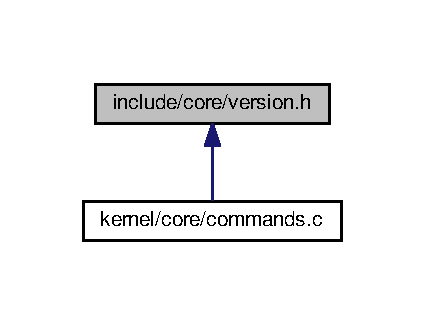
\includegraphics[width=204pt]{version_8h__dep__incl}
\end{center}
\end{figure}
\subsection*{Macros}
\begin{DoxyCompactItemize}
\item 
\#define \hyperlink{version_8h_a8ee42974be7bd483db95ede8d81be518}{O\+S\+\_\+\+V\+E\+R\+S\+I\+ON}~((const char$\ast$) \char`\"{}N\+PE-\/M\+P\+X.\+R5.\+04282017\char`\"{})
\end{DoxyCompactItemize}


\subsection{Macro Definition Documentation}
\index{version.\+h@{version.\+h}!O\+S\+\_\+\+V\+E\+R\+S\+I\+ON@{O\+S\+\_\+\+V\+E\+R\+S\+I\+ON}}
\index{O\+S\+\_\+\+V\+E\+R\+S\+I\+ON@{O\+S\+\_\+\+V\+E\+R\+S\+I\+ON}!version.\+h@{version.\+h}}
\subsubsection[{\texorpdfstring{O\+S\+\_\+\+V\+E\+R\+S\+I\+ON}{OS_VERSION}}]{\setlength{\rightskip}{0pt plus 5cm}\#define O\+S\+\_\+\+V\+E\+R\+S\+I\+ON~((const char$\ast$) \char`\"{}N\+PE-\/M\+P\+X.\+R5.\+04282017\char`\"{})}\hypertarget{version_8h_a8ee42974be7bd483db95ede8d81be518}{}\label{version_8h_a8ee42974be7bd483db95ede8d81be518}
The current OS version. 
\hypertarget{math_8h}{}\section{include/math.h File Reference}
\label{math_8h}\index{include/math.\+h@{include/math.\+h}}
This graph shows which files directly or indirectly include this file\+:\nopagebreak
\begin{figure}[H]
\begin{center}
\leavevmode
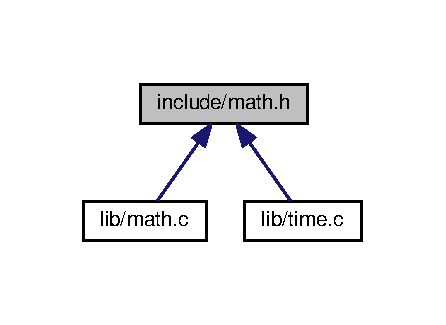
\includegraphics[width=214pt]{math_8h__dep__incl}
\end{center}
\end{figure}
\subsection*{Functions}
\begin{DoxyCompactItemize}
\item 
unsigned char \hyperlink{math_8h_a844e84db974b1f32caabf109e83a33e5}{bcd\+To\+Dec} (unsigned char bcd)
\item 
unsigned char \hyperlink{math_8h_ab92bb5c05ba791a72094f439f4fe3aa4}{dec\+To\+Bcd} (unsigned char dec)
\end{DoxyCompactItemize}


\subsection{Function Documentation}
\index{math.\+h@{math.\+h}!bcd\+To\+Dec@{bcd\+To\+Dec}}
\index{bcd\+To\+Dec@{bcd\+To\+Dec}!math.\+h@{math.\+h}}
\subsubsection[{\texorpdfstring{bcd\+To\+Dec(unsigned char bcd)}{bcdToDec(unsigned char bcd)}}]{\setlength{\rightskip}{0pt plus 5cm}unsigned char bcd\+To\+Dec (
\begin{DoxyParamCaption}
\item[{unsigned char}]{bcd}
\end{DoxyParamCaption}
)}\hypertarget{math_8h_a844e84db974b1f32caabf109e83a33e5}{}\label{math_8h_a844e84db974b1f32caabf109e83a33e5}
Converts a B\+CD encoded byte to a decimal encoded byte


\begin{DoxyParams}{Parameters}
{\em bcd} & The value to convert \\
\hline
\end{DoxyParams}
\begin{DoxyReturn}{Returns}
The decimal value 
\end{DoxyReturn}
\index{math.\+h@{math.\+h}!dec\+To\+Bcd@{dec\+To\+Bcd}}
\index{dec\+To\+Bcd@{dec\+To\+Bcd}!math.\+h@{math.\+h}}
\subsubsection[{\texorpdfstring{dec\+To\+Bcd(unsigned char dec)}{decToBcd(unsigned char dec)}}]{\setlength{\rightskip}{0pt plus 5cm}unsigned char dec\+To\+Bcd (
\begin{DoxyParamCaption}
\item[{unsigned char}]{dec}
\end{DoxyParamCaption}
)}\hypertarget{math_8h_ab92bb5c05ba791a72094f439f4fe3aa4}{}\label{math_8h_ab92bb5c05ba791a72094f439f4fe3aa4}
Converts a decimal encoded byte to a B\+CD encoded byte


\begin{DoxyParams}{Parameters}
{\em dec} & The value to convert \\
\hline
\end{DoxyParams}
\begin{DoxyReturn}{Returns}
The B\+CD value 
\end{DoxyReturn}

\hypertarget{heap_8h}{}\section{include/mem/heap.h File Reference}
\label{heap_8h}\index{include/mem/heap.\+h@{include/mem/heap.\+h}}
This graph shows which files directly or indirectly include this file\+:\nopagebreak
\begin{figure}[H]
\begin{center}
\leavevmode
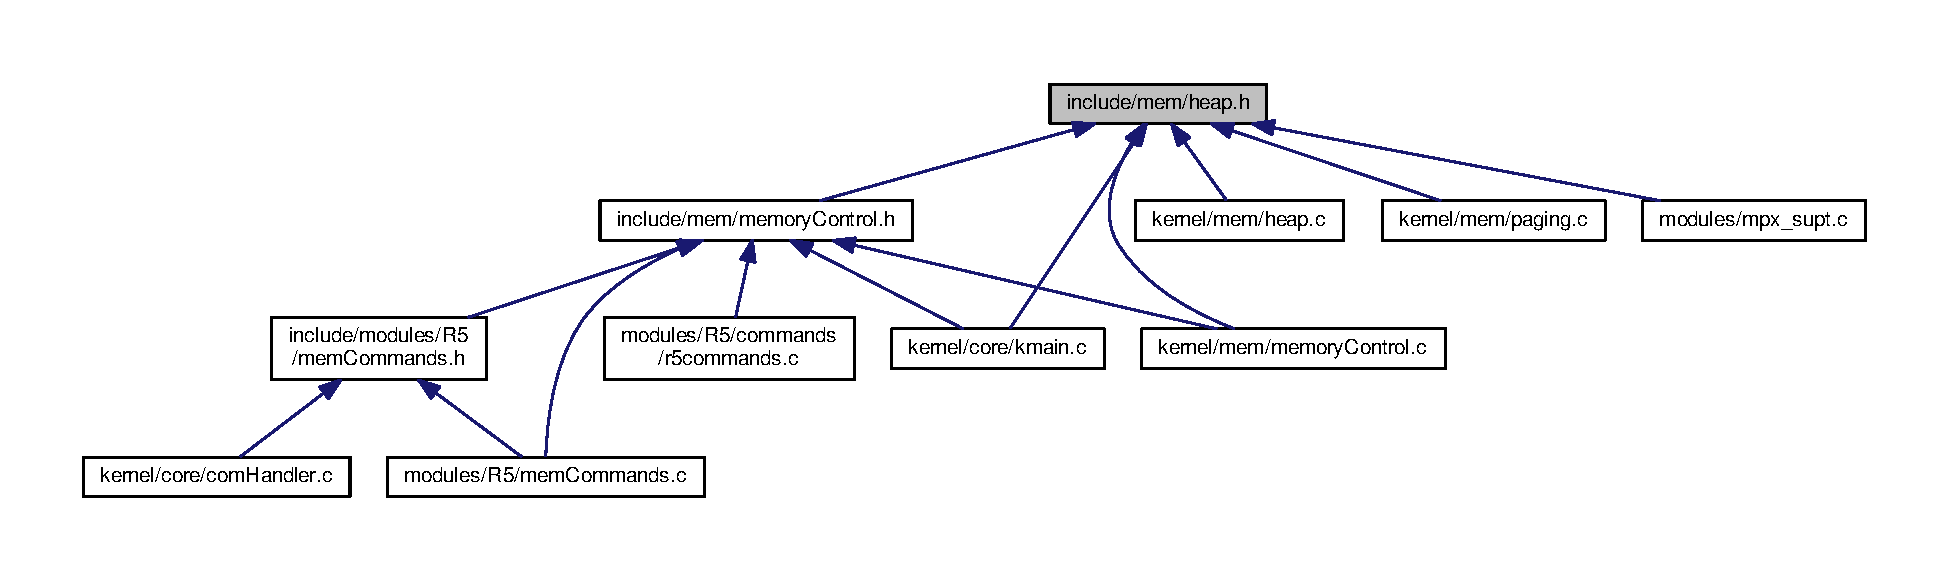
\includegraphics[width=350pt]{heap_8h__dep__incl}
\end{center}
\end{figure}
\subsection*{Data Structures}
\begin{DoxyCompactItemize}
\item 
struct \hyperlink{structheader}{header}
\item 
struct \hyperlink{structfooter}{footer}
\item 
struct \hyperlink{structindex__entry}{index\+\_\+entry}
\item 
struct \hyperlink{structindex__table}{index\+\_\+table}
\item 
struct \hyperlink{structheap}{heap}
\end{DoxyCompactItemize}
\subsection*{Macros}
\begin{DoxyCompactItemize}
\item 
\#define \hyperlink{heap_8h_a032503e76d6f69bc67e99e909c8125da}{T\+A\+B\+L\+E\+\_\+\+S\+I\+ZE}~0x1000
\item 
\#define \hyperlink{heap_8h_a15073b9742f7e29d8174509197eb4ab9}{K\+H\+E\+A\+P\+\_\+\+B\+A\+SE}~0x\+D000000
\item 
\#define \hyperlink{heap_8h_aee52619f74498ad224eb8e4354b89e40}{K\+H\+E\+A\+P\+\_\+\+M\+IN}~0x10000
\item 
\#define \hyperlink{heap_8h_a0f2696767a10e6efffc64e9b459c4ea6}{K\+H\+E\+A\+P\+\_\+\+S\+I\+ZE}~0x1000000
\end{DoxyCompactItemize}
\subsection*{Functions}
\begin{DoxyCompactItemize}
\item 
\hyperlink{system_8h_a757de76cafbcddaac0d1632902fe4cb8}{u32int} \hyperlink{heap_8h_a9bfb8053c2382598ef5b2175f475d49a}{\+\_\+kmalloc} (\hyperlink{system_8h_a757de76cafbcddaac0d1632902fe4cb8}{u32int} size, int align, \hyperlink{system_8h_a757de76cafbcddaac0d1632902fe4cb8}{u32int} $\ast$phys\+\_\+addr)
\item 
\hyperlink{system_8h_a757de76cafbcddaac0d1632902fe4cb8}{u32int} \hyperlink{heap_8h_a15d6a52c5c080c8c7ffc73e336d8e574}{kmalloc} (\hyperlink{system_8h_a757de76cafbcddaac0d1632902fe4cb8}{u32int} size)
\item 
\hyperlink{system_8h_a757de76cafbcddaac0d1632902fe4cb8}{u32int} \hyperlink{heap_8h_aa2a6fb2aa05727dc1e7d72cbc108e63c}{kfree} ()
\item 
void \hyperlink{heap_8h_a755a69ff831b6e23a808dcf4b9944854}{init\+\_\+kheap} ()
\item 
\hyperlink{system_8h_a757de76cafbcddaac0d1632902fe4cb8}{u32int} \hyperlink{heap_8h_a2b1d5a9ba11695605f74fc10cd719af5}{alloc} (\hyperlink{system_8h_a757de76cafbcddaac0d1632902fe4cb8}{u32int} size, \hyperlink{structheap}{heap} $\ast$hp, int align)
\item 
\hyperlink{structheap}{heap} $\ast$ \hyperlink{heap_8h_a686135c02695aef4208f93d4549a15d0}{make\+\_\+heap} (\hyperlink{system_8h_a757de76cafbcddaac0d1632902fe4cb8}{u32int} \hyperlink{tables_8h_ab5763c2b18c825c8b8fba44b2e60ddc1}{base}, \hyperlink{system_8h_a757de76cafbcddaac0d1632902fe4cb8}{u32int} max, \hyperlink{system_8h_a757de76cafbcddaac0d1632902fe4cb8}{u32int} min)
\end{DoxyCompactItemize}
\subsection*{Variables}
\begin{DoxyCompactItemize}
\item 
typedef \hyperlink{heap_8h_aaa4b117a86b9205e66f2cde318c1f01e}{\+\_\+\+\_\+attribute\+\_\+\+\_\+}
\end{DoxyCompactItemize}


\subsection{Macro Definition Documentation}
\index{heap.\+h@{heap.\+h}!K\+H\+E\+A\+P\+\_\+\+B\+A\+SE@{K\+H\+E\+A\+P\+\_\+\+B\+A\+SE}}
\index{K\+H\+E\+A\+P\+\_\+\+B\+A\+SE@{K\+H\+E\+A\+P\+\_\+\+B\+A\+SE}!heap.\+h@{heap.\+h}}
\subsubsection[{\texorpdfstring{K\+H\+E\+A\+P\+\_\+\+B\+A\+SE}{KHEAP_BASE}}]{\setlength{\rightskip}{0pt plus 5cm}\#define K\+H\+E\+A\+P\+\_\+\+B\+A\+SE~0x\+D000000}\hypertarget{heap_8h_a15073b9742f7e29d8174509197eb4ab9}{}\label{heap_8h_a15073b9742f7e29d8174509197eb4ab9}
\index{heap.\+h@{heap.\+h}!K\+H\+E\+A\+P\+\_\+\+M\+IN@{K\+H\+E\+A\+P\+\_\+\+M\+IN}}
\index{K\+H\+E\+A\+P\+\_\+\+M\+IN@{K\+H\+E\+A\+P\+\_\+\+M\+IN}!heap.\+h@{heap.\+h}}
\subsubsection[{\texorpdfstring{K\+H\+E\+A\+P\+\_\+\+M\+IN}{KHEAP_MIN}}]{\setlength{\rightskip}{0pt plus 5cm}\#define K\+H\+E\+A\+P\+\_\+\+M\+IN~0x10000}\hypertarget{heap_8h_aee52619f74498ad224eb8e4354b89e40}{}\label{heap_8h_aee52619f74498ad224eb8e4354b89e40}
\index{heap.\+h@{heap.\+h}!K\+H\+E\+A\+P\+\_\+\+S\+I\+ZE@{K\+H\+E\+A\+P\+\_\+\+S\+I\+ZE}}
\index{K\+H\+E\+A\+P\+\_\+\+S\+I\+ZE@{K\+H\+E\+A\+P\+\_\+\+S\+I\+ZE}!heap.\+h@{heap.\+h}}
\subsubsection[{\texorpdfstring{K\+H\+E\+A\+P\+\_\+\+S\+I\+ZE}{KHEAP_SIZE}}]{\setlength{\rightskip}{0pt plus 5cm}\#define K\+H\+E\+A\+P\+\_\+\+S\+I\+ZE~0x1000000}\hypertarget{heap_8h_a0f2696767a10e6efffc64e9b459c4ea6}{}\label{heap_8h_a0f2696767a10e6efffc64e9b459c4ea6}
\index{heap.\+h@{heap.\+h}!T\+A\+B\+L\+E\+\_\+\+S\+I\+ZE@{T\+A\+B\+L\+E\+\_\+\+S\+I\+ZE}}
\index{T\+A\+B\+L\+E\+\_\+\+S\+I\+ZE@{T\+A\+B\+L\+E\+\_\+\+S\+I\+ZE}!heap.\+h@{heap.\+h}}
\subsubsection[{\texorpdfstring{T\+A\+B\+L\+E\+\_\+\+S\+I\+ZE}{TABLE_SIZE}}]{\setlength{\rightskip}{0pt plus 5cm}\#define T\+A\+B\+L\+E\+\_\+\+S\+I\+ZE~0x1000}\hypertarget{heap_8h_a032503e76d6f69bc67e99e909c8125da}{}\label{heap_8h_a032503e76d6f69bc67e99e909c8125da}
Kernel heap. 

\subsection{Function Documentation}
\index{heap.\+h@{heap.\+h}!\+\_\+kmalloc@{\+\_\+kmalloc}}
\index{\+\_\+kmalloc@{\+\_\+kmalloc}!heap.\+h@{heap.\+h}}
\subsubsection[{\texorpdfstring{\+\_\+kmalloc(u32int size, int align, u32int $\ast$phys\+\_\+addr)}{_kmalloc(u32int size, int align, u32int *phys_addr)}}]{\setlength{\rightskip}{0pt plus 5cm}{\bf u32int} \+\_\+kmalloc (
\begin{DoxyParamCaption}
\item[{{\bf u32int}}]{size, }
\item[{int}]{page\+\_\+align, }
\item[{{\bf u32int} $\ast$}]{phys\+\_\+addr}
\end{DoxyParamCaption}
)}\hypertarget{heap_8h_a9bfb8053c2382598ef5b2175f475d49a}{}\label{heap_8h_a9bfb8053c2382598ef5b2175f475d49a}
Base-\/level kernel memory allocation routine. Used to provide page alignment and access physical addresses of allocations. Called by kmalloc with align=0, physical\+\_\+address=0.


\begin{DoxyParams}{Parameters}
{\em size} & The amount of memory to allocate \\
\hline
{\em align} & The page alignment \\
\hline
{\em phys\+\_\+addr} & The physical address \\
\hline
\end{DoxyParams}
\begin{DoxyReturn}{Returns}
The memory address 
\end{DoxyReturn}
\index{heap.\+h@{heap.\+h}!alloc@{alloc}}
\index{alloc@{alloc}!heap.\+h@{heap.\+h}}
\subsubsection[{\texorpdfstring{alloc(u32int size, heap $\ast$hp, int align)}{alloc(u32int size, heap *hp, int align)}}]{\setlength{\rightskip}{0pt plus 5cm}{\bf u32int} alloc (
\begin{DoxyParamCaption}
\item[{{\bf u32int}}]{size, }
\item[{{\bf heap} $\ast$}]{h, }
\item[{int}]{align}
\end{DoxyParamCaption}
)}\hypertarget{heap_8h_a2b1d5a9ba11695605f74fc10cd719af5}{}\label{heap_8h_a2b1d5a9ba11695605f74fc10cd719af5}
Allocates some memory using the given heap. Can specify page-\/alignment.


\begin{DoxyParams}{Parameters}
{\em size} & The amount of memory to allocate \\
\hline
{\em hp} & The heap to allocate on \\
\hline
{\em align} & The page alignment \\
\hline
\end{DoxyParams}
\begin{DoxyReturn}{Returns}
The memory address 
\end{DoxyReturn}
\index{heap.\+h@{heap.\+h}!init\+\_\+kheap@{init\+\_\+kheap}}
\index{init\+\_\+kheap@{init\+\_\+kheap}!heap.\+h@{heap.\+h}}
\subsubsection[{\texorpdfstring{init\+\_\+kheap()}{init_kheap()}}]{\setlength{\rightskip}{0pt plus 5cm}void init\+\_\+kheap (
\begin{DoxyParamCaption}
{}
\end{DoxyParamCaption}
)}\hypertarget{heap_8h_a755a69ff831b6e23a808dcf4b9944854}{}\label{heap_8h_a755a69ff831b6e23a808dcf4b9944854}
Initialize the kernel heap, and set it as the current heap. \index{heap.\+h@{heap.\+h}!kfree@{kfree}}
\index{kfree@{kfree}!heap.\+h@{heap.\+h}}
\subsubsection[{\texorpdfstring{kfree()}{kfree()}}]{\setlength{\rightskip}{0pt plus 5cm}{\bf u32int} kfree (
\begin{DoxyParamCaption}
{}
\end{DoxyParamCaption}
)}\hypertarget{heap_8h_aa2a6fb2aa05727dc1e7d72cbc108e63c}{}\label{heap_8h_aa2a6fb2aa05727dc1e7d72cbc108e63c}
Free kernel memory.

\begin{DoxyReturn}{Returns}

\end{DoxyReturn}
\index{heap.\+h@{heap.\+h}!kmalloc@{kmalloc}}
\index{kmalloc@{kmalloc}!heap.\+h@{heap.\+h}}
\subsubsection[{\texorpdfstring{kmalloc(u32int size)}{kmalloc(u32int size)}}]{\setlength{\rightskip}{0pt plus 5cm}{\bf u32int} kmalloc (
\begin{DoxyParamCaption}
\item[{{\bf u32int}}]{size}
\end{DoxyParamCaption}
)}\hypertarget{heap_8h_a15d6a52c5c080c8c7ffc73e336d8e574}{}\label{heap_8h_a15d6a52c5c080c8c7ffc73e336d8e574}
Standard memory allocation routine. Use this unless you need to specify alignment or obtain a physical address. Calls \+\_\+kmalloc.


\begin{DoxyParams}{Parameters}
{\em size} & The amount of memory to allocate \\
\hline
\end{DoxyParams}
\begin{DoxyReturn}{Returns}
The memory address 
\end{DoxyReturn}
\index{heap.\+h@{heap.\+h}!make\+\_\+heap@{make\+\_\+heap}}
\index{make\+\_\+heap@{make\+\_\+heap}!heap.\+h@{heap.\+h}}
\subsubsection[{\texorpdfstring{make\+\_\+heap(u32int base, u32int max, u32int min)}{make_heap(u32int base, u32int max, u32int min)}}]{\setlength{\rightskip}{0pt plus 5cm}{\bf heap}$\ast$ make\+\_\+heap (
\begin{DoxyParamCaption}
\item[{{\bf u32int}}]{base, }
\item[{{\bf u32int}}]{max, }
\item[{{\bf u32int}}]{min}
\end{DoxyParamCaption}
)}\hypertarget{heap_8h_a686135c02695aef4208f93d4549a15d0}{}\label{heap_8h_a686135c02695aef4208f93d4549a15d0}
Create a new heap.


\begin{DoxyParams}{Parameters}
{\em base} & Physical start address of the heap \\
\hline
{\em max} & Maximum size the heap may grow to \\
\hline
{\em min} & Minium/\+Initial size \\
\hline
\end{DoxyParams}
\begin{DoxyReturn}{Returns}
The address of the heap 
\end{DoxyReturn}


\subsection{Variable Documentation}
\index{heap.\+h@{heap.\+h}!\+\_\+\+\_\+attribute\+\_\+\+\_\+@{\+\_\+\+\_\+attribute\+\_\+\+\_\+}}
\index{\+\_\+\+\_\+attribute\+\_\+\+\_\+@{\+\_\+\+\_\+attribute\+\_\+\+\_\+}!heap.\+h@{heap.\+h}}
\subsubsection[{\texorpdfstring{\+\_\+\+\_\+attribute\+\_\+\+\_\+}{__attribute__}}]{\setlength{\rightskip}{0pt plus 5cm}struct {\bf gdt\+\_\+entry\+\_\+struct} \+\_\+\+\_\+attribute\+\_\+\+\_\+}\hypertarget{heap_8h_aaa4b117a86b9205e66f2cde318c1f01e}{}\label{heap_8h_aaa4b117a86b9205e66f2cde318c1f01e}

\hypertarget{memory_control_8h}{}\section{include/mem/memory\+Control.h File Reference}
\label{memory_control_8h}\index{include/mem/memory\+Control.\+h@{include/mem/memory\+Control.\+h}}
{\ttfamily \#include $<$system.\+h$>$}\\*
{\ttfamily \#include $<$mem/heap.\+h$>$}\\*
{\ttfamily \#include $<$modules/mpx\+\_\+supt.\+h$>$}\\*
{\ttfamily \#include $<$boolean.\+h$>$}\\*
Include dependency graph for memory\+Control.\+h\+:\nopagebreak
\begin{figure}[H]
\begin{center}
\leavevmode
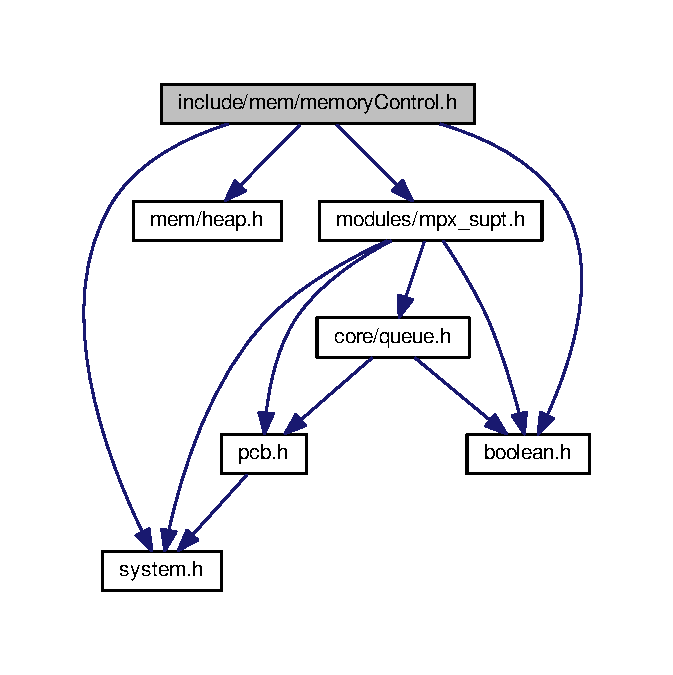
\includegraphics[width=323pt]{memory_control_8h__incl}
\end{center}
\end{figure}
This graph shows which files directly or indirectly include this file\+:\nopagebreak
\begin{figure}[H]
\begin{center}
\leavevmode
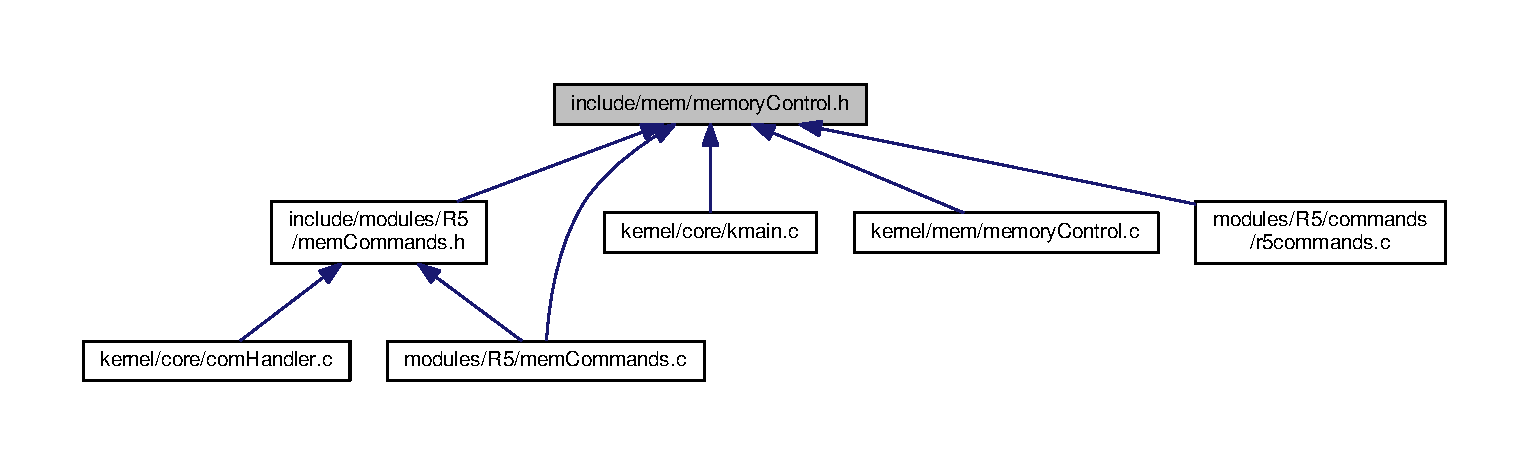
\includegraphics[width=350pt]{memory_control_8h__dep__incl}
\end{center}
\end{figure}
\subsection*{Data Structures}
\begin{DoxyCompactItemize}
\item 
struct \hyperlink{structcmcb}{cmcb}
\item 
struct \hyperlink{structlmcb}{lmcb}
\end{DoxyCompactItemize}
\subsection*{Macros}
\begin{DoxyCompactItemize}
\item 
\#define \hyperlink{memory_control_8h_a9a8e700d56e7d858108b755ad3edb52e}{F\+R\+EE}~0
\item 
\#define \hyperlink{memory_control_8h_aaa0db48d5bc1e51c3fde24e3b8ade641}{A\+L\+L\+O\+C\+A\+T\+ED}~1
\end{DoxyCompactItemize}
\subsection*{Typedefs}
\begin{DoxyCompactItemize}
\item 
typedef struct \hyperlink{structcmcb}{cmcb} \hyperlink{memory_control_8h_ad874ed0d8f386f5de2010c7f3624d077}{cmcb}
\item 
typedef struct \hyperlink{structlmcb}{lmcb} \hyperlink{memory_control_8h_a63ec758f80a50b22328b902eb98d9844}{lmcb}
\end{DoxyCompactItemize}
\subsection*{Functions}
\begin{DoxyCompactItemize}
\item 
\hyperlink{boolean_8h_a7c6368b321bd9acd0149b030bb8275ed}{boolean} \hyperlink{memory_control_8h_af9f876f6d6cea9ef14b5c457f8835ab1}{initialize\+Heap} (int size)
\item 
void $\ast$ \hyperlink{memory_control_8h_ae841b4b92ac63a904d3b357cd0277a0e}{allocate\+Memory} (int size)
\item 
\hyperlink{boolean_8h_a7c6368b321bd9acd0149b030bb8275ed}{boolean} \hyperlink{memory_control_8h_af17f3ec8ec711d793814e7afb5fb416b}{deallocate\+Memory} (void $\ast$mem\+Pointer)
\item 
\hyperlink{boolean_8h_a7c6368b321bd9acd0149b030bb8275ed}{boolean} \hyperlink{memory_control_8h_aa71d41fd3d95c354d4d5e922c6c21210}{is\+Empty} ()
\item 
\hyperlink{structcmcb}{cmcb} $\ast$ \hyperlink{memory_control_8h_aa8d430c05a8323b5f5570e4f000d033b}{get\+Free\+Head} ()
\item 
\hyperlink{structcmcb}{cmcb} $\ast$ \hyperlink{memory_control_8h_a5bf2a856d94db1ea1af87b4dcf95b830}{get\+Allocated\+Head} ()
\end{DoxyCompactItemize}


\subsection{Macro Definition Documentation}
\index{memory\+Control.\+h@{memory\+Control.\+h}!A\+L\+L\+O\+C\+A\+T\+ED@{A\+L\+L\+O\+C\+A\+T\+ED}}
\index{A\+L\+L\+O\+C\+A\+T\+ED@{A\+L\+L\+O\+C\+A\+T\+ED}!memory\+Control.\+h@{memory\+Control.\+h}}
\subsubsection[{\texorpdfstring{A\+L\+L\+O\+C\+A\+T\+ED}{ALLOCATED}}]{\setlength{\rightskip}{0pt plus 5cm}\#define A\+L\+L\+O\+C\+A\+T\+ED~1}\hypertarget{memory_control_8h_aaa0db48d5bc1e51c3fde24e3b8ade641}{}\label{memory_control_8h_aaa0db48d5bc1e51c3fde24e3b8ade641}
\index{memory\+Control.\+h@{memory\+Control.\+h}!F\+R\+EE@{F\+R\+EE}}
\index{F\+R\+EE@{F\+R\+EE}!memory\+Control.\+h@{memory\+Control.\+h}}
\subsubsection[{\texorpdfstring{F\+R\+EE}{FREE}}]{\setlength{\rightskip}{0pt plus 5cm}\#define F\+R\+EE~0}\hypertarget{memory_control_8h_a9a8e700d56e7d858108b755ad3edb52e}{}\label{memory_control_8h_a9a8e700d56e7d858108b755ad3edb52e}


\subsection{Typedef Documentation}
\index{memory\+Control.\+h@{memory\+Control.\+h}!cmcb@{cmcb}}
\index{cmcb@{cmcb}!memory\+Control.\+h@{memory\+Control.\+h}}
\subsubsection[{\texorpdfstring{cmcb}{cmcb}}]{\setlength{\rightskip}{0pt plus 5cm}typedef struct {\bf cmcb}  {\bf cmcb}}\hypertarget{memory_control_8h_ad874ed0d8f386f5de2010c7f3624d077}{}\label{memory_control_8h_ad874ed0d8f386f5de2010c7f3624d077}
\index{memory\+Control.\+h@{memory\+Control.\+h}!lmcb@{lmcb}}
\index{lmcb@{lmcb}!memory\+Control.\+h@{memory\+Control.\+h}}
\subsubsection[{\texorpdfstring{lmcb}{lmcb}}]{\setlength{\rightskip}{0pt plus 5cm}typedef struct {\bf lmcb}  {\bf lmcb}}\hypertarget{memory_control_8h_a63ec758f80a50b22328b902eb98d9844}{}\label{memory_control_8h_a63ec758f80a50b22328b902eb98d9844}


\subsection{Function Documentation}
\index{memory\+Control.\+h@{memory\+Control.\+h}!allocate\+Memory@{allocate\+Memory}}
\index{allocate\+Memory@{allocate\+Memory}!memory\+Control.\+h@{memory\+Control.\+h}}
\subsubsection[{\texorpdfstring{allocate\+Memory(int size)}{allocateMemory(int size)}}]{\setlength{\rightskip}{0pt plus 5cm}void$\ast$ allocate\+Memory (
\begin{DoxyParamCaption}
\item[{int}]{size}
\end{DoxyParamCaption}
)}\hypertarget{memory_control_8h_ae841b4b92ac63a904d3b357cd0277a0e}{}\label{memory_control_8h_ae841b4b92ac63a904d3b357cd0277a0e}
Allocates a memory block if enough memory is availabel


\begin{DoxyParams}{Parameters}
{\em size} & -\/ size of memory to allocate in bytes \\
\hline
\end{DoxyParams}
\begin{DoxyReturn}{Returns}
pointer to the me 
\end{DoxyReturn}
\index{memory\+Control.\+h@{memory\+Control.\+h}!deallocate\+Memory@{deallocate\+Memory}}
\index{deallocate\+Memory@{deallocate\+Memory}!memory\+Control.\+h@{memory\+Control.\+h}}
\subsubsection[{\texorpdfstring{deallocate\+Memory(void $\ast$mem\+Pointer)}{deallocateMemory(void *memPointer)}}]{\setlength{\rightskip}{0pt plus 5cm}{\bf boolean} deallocate\+Memory (
\begin{DoxyParamCaption}
\item[{void $\ast$}]{mem\+Pointer}
\end{DoxyParamCaption}
)}\hypertarget{memory_control_8h_af17f3ec8ec711d793814e7afb5fb416b}{}\label{memory_control_8h_af17f3ec8ec711d793814e7afb5fb416b}
Deallocates the block of memory at the mempointer


\begin{DoxyParams}{Parameters}
{\em mem\+Pointer} & -\/ pointer to the mem block \\
\hline
\end{DoxyParams}
\begin{DoxyReturn}{Returns}
boolean -\/ tells whether successfull dealloc
\end{DoxyReturn}
Deallocates the block of memory at the mempointer


\begin{DoxyParams}{Parameters}
{\em mem\+Pointer} & -\/ pointer to the mem block \\
\hline
\end{DoxyParams}
\begin{DoxyReturn}{Returns}
boolean -\/ boolean telling whether succesful dealloc 
\end{DoxyReturn}
\index{memory\+Control.\+h@{memory\+Control.\+h}!get\+Allocated\+Head@{get\+Allocated\+Head}}
\index{get\+Allocated\+Head@{get\+Allocated\+Head}!memory\+Control.\+h@{memory\+Control.\+h}}
\subsubsection[{\texorpdfstring{get\+Allocated\+Head()}{getAllocatedHead()}}]{\setlength{\rightskip}{0pt plus 5cm}{\bf cmcb}$\ast$ get\+Allocated\+Head (
\begin{DoxyParamCaption}
{}
\end{DoxyParamCaption}
)}\hypertarget{memory_control_8h_a5bf2a856d94db1ea1af87b4dcf95b830}{}\label{memory_control_8h_a5bf2a856d94db1ea1af87b4dcf95b830}
Returns the head to the allocated list

\begin{DoxyReturn}{Returns}
cmcb $\ast$ to the allocated list head 
\end{DoxyReturn}
\index{memory\+Control.\+h@{memory\+Control.\+h}!get\+Free\+Head@{get\+Free\+Head}}
\index{get\+Free\+Head@{get\+Free\+Head}!memory\+Control.\+h@{memory\+Control.\+h}}
\subsubsection[{\texorpdfstring{get\+Free\+Head()}{getFreeHead()}}]{\setlength{\rightskip}{0pt plus 5cm}{\bf cmcb}$\ast$ get\+Free\+Head (
\begin{DoxyParamCaption}
{}
\end{DoxyParamCaption}
)}\hypertarget{memory_control_8h_aa8d430c05a8323b5f5570e4f000d033b}{}\label{memory_control_8h_aa8d430c05a8323b5f5570e4f000d033b}
Returns the head of the free list

\begin{DoxyReturn}{Returns}
cmcb $\ast$ to the free list head 
\end{DoxyReturn}
\index{memory\+Control.\+h@{memory\+Control.\+h}!initialize\+Heap@{initialize\+Heap}}
\index{initialize\+Heap@{initialize\+Heap}!memory\+Control.\+h@{memory\+Control.\+h}}
\subsubsection[{\texorpdfstring{initialize\+Heap(int size)}{initializeHeap(int size)}}]{\setlength{\rightskip}{0pt plus 5cm}{\bf boolean} initialize\+Heap (
\begin{DoxyParamCaption}
\item[{int}]{size}
\end{DoxyParamCaption}
)}\hypertarget{memory_control_8h_af9f876f6d6cea9ef14b5c457f8835ab1}{}\label{memory_control_8h_af9f876f6d6cea9ef14b5c457f8835ab1}
Initializes the heap to the provided size and creates a free mem block across it


\begin{DoxyParams}{Parameters}
{\em size} & -\/ size of heap in bytes \\
\hline
\end{DoxyParams}
\begin{DoxyReturn}{Returns}
boolean -\/ boolean denoting if heap was initialized 
\end{DoxyReturn}
\index{memory\+Control.\+h@{memory\+Control.\+h}!is\+Empty@{is\+Empty}}
\index{is\+Empty@{is\+Empty}!memory\+Control.\+h@{memory\+Control.\+h}}
\subsubsection[{\texorpdfstring{is\+Empty()}{isEmpty()}}]{\setlength{\rightskip}{0pt plus 5cm}{\bf boolean} is\+Empty (
\begin{DoxyParamCaption}
{}
\end{DoxyParamCaption}
)}\hypertarget{memory_control_8h_aa71d41fd3d95c354d4d5e922c6c21210}{}\label{memory_control_8h_aa71d41fd3d95c354d4d5e922c6c21210}
Returns a boolean telling if all the memory is empty

\begin{DoxyReturn}{Returns}
boolean 
\end{DoxyReturn}

\hypertarget{paging_8h}{}\section{include/mem/paging.h File Reference}
\label{paging_8h}\index{include/mem/paging.\+h@{include/mem/paging.\+h}}
{\ttfamily \#include $<$system.\+h$>$}\\*
Include dependency graph for paging.\+h\+:\nopagebreak
\begin{figure}[H]
\begin{center}
\leavevmode
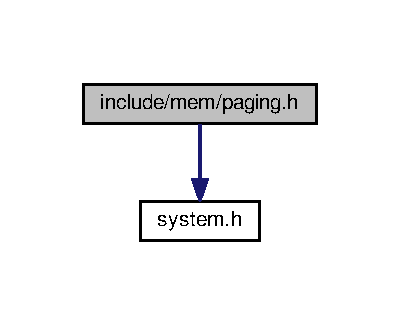
\includegraphics[width=192pt]{paging_8h__incl}
\end{center}
\end{figure}
This graph shows which files directly or indirectly include this file\+:\nopagebreak
\begin{figure}[H]
\begin{center}
\leavevmode
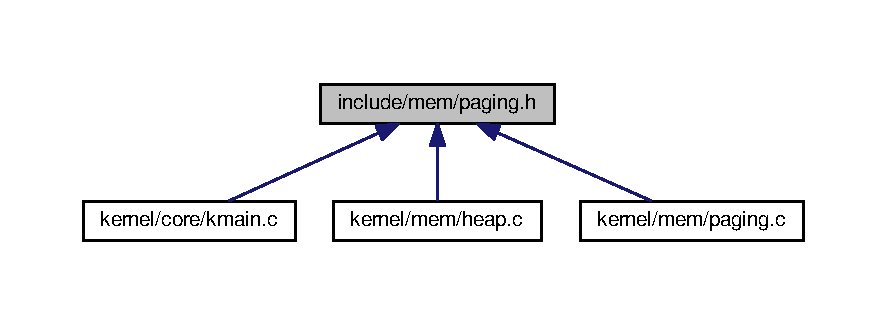
\includegraphics[width=350pt]{paging_8h__dep__incl}
\end{center}
\end{figure}
\subsection*{Data Structures}
\begin{DoxyCompactItemize}
\item 
struct \hyperlink{structpage__entry}{page\+\_\+entry}
\item 
struct \hyperlink{structpage__table}{page\+\_\+table}
\item 
struct \hyperlink{structpage__dir}{page\+\_\+dir}
\end{DoxyCompactItemize}
\subsection*{Macros}
\begin{DoxyCompactItemize}
\item 
\#define \hyperlink{paging_8h_a7d467c1d283fdfa1f2081ba1e0d01b6e}{P\+A\+G\+E\+\_\+\+S\+I\+ZE}~0x1000
\end{DoxyCompactItemize}
\subsection*{Functions}
\begin{DoxyCompactItemize}
\item 
void \hyperlink{paging_8h_a70101fc152ff58caafbe36ab391a9a68}{set\+\_\+bit} (\hyperlink{system_8h_a757de76cafbcddaac0d1632902fe4cb8}{u32int} addr)
\item 
void \hyperlink{paging_8h_adcef508c82c20a032508f871e79e1b92}{clear\+\_\+bit} (\hyperlink{system_8h_a757de76cafbcddaac0d1632902fe4cb8}{u32int} addr)
\item 
\hyperlink{system_8h_a757de76cafbcddaac0d1632902fe4cb8}{u32int} \hyperlink{paging_8h_a317b4797bc81f65bd01cfa190800ecdd}{get\+\_\+bit} (\hyperlink{system_8h_a757de76cafbcddaac0d1632902fe4cb8}{u32int} addr)
\item 
\hyperlink{system_8h_a757de76cafbcddaac0d1632902fe4cb8}{u32int} \hyperlink{paging_8h_acb3c25257061521382c7ba900c1c1ab4}{first\+\_\+free} ()
\item 
void \hyperlink{paging_8h_a919b727f386797a8b9d8eceb5c4e7313}{init\+\_\+paging} ()
\item 
void \hyperlink{paging_8h_a3affceba4cd194e1c516404c14abbe7c}{load\+\_\+page\+\_\+dir} (\hyperlink{structpage__dir}{page\+\_\+dir} $\ast$new\+\_\+page\+\_\+dir)
\item 
\hyperlink{structpage__entry}{page\+\_\+entry} $\ast$ \hyperlink{paging_8h_a69b165b3d1adf3aeaae126ca7a5aac3e}{get\+\_\+page} (\hyperlink{system_8h_a757de76cafbcddaac0d1632902fe4cb8}{u32int} addr, \hyperlink{structpage__dir}{page\+\_\+dir} $\ast$dir, int make\+\_\+table)
\item 
void \hyperlink{paging_8h_a04bce9da2c1d7c59f6efd8e4d9b54db7}{new\+\_\+frame} (\hyperlink{structpage__entry}{page\+\_\+entry} $\ast$page)
\end{DoxyCompactItemize}


\subsection{Macro Definition Documentation}
\index{paging.\+h@{paging.\+h}!P\+A\+G\+E\+\_\+\+S\+I\+ZE@{P\+A\+G\+E\+\_\+\+S\+I\+ZE}}
\index{P\+A\+G\+E\+\_\+\+S\+I\+ZE@{P\+A\+G\+E\+\_\+\+S\+I\+ZE}!paging.\+h@{paging.\+h}}
\subsubsection[{\texorpdfstring{P\+A\+G\+E\+\_\+\+S\+I\+ZE}{PAGE_SIZE}}]{\setlength{\rightskip}{0pt plus 5cm}\#define P\+A\+G\+E\+\_\+\+S\+I\+ZE~0x1000}\hypertarget{paging_8h_a7d467c1d283fdfa1f2081ba1e0d01b6e}{}\label{paging_8h_a7d467c1d283fdfa1f2081ba1e0d01b6e}


\subsection{Function Documentation}
\index{paging.\+h@{paging.\+h}!clear\+\_\+bit@{clear\+\_\+bit}}
\index{clear\+\_\+bit@{clear\+\_\+bit}!paging.\+h@{paging.\+h}}
\subsubsection[{\texorpdfstring{clear\+\_\+bit(u32int addr)}{clear_bit(u32int addr)}}]{\setlength{\rightskip}{0pt plus 5cm}void clear\+\_\+bit (
\begin{DoxyParamCaption}
\item[{{\bf u32int}}]{addr}
\end{DoxyParamCaption}
)}\hypertarget{paging_8h_adcef508c82c20a032508f871e79e1b92}{}\label{paging_8h_adcef508c82c20a032508f871e79e1b92}
Marks a page frame bit as free (0).


\begin{DoxyParams}{Parameters}
{\em addr} & The address of the frame \\
\hline
\end{DoxyParams}
\index{paging.\+h@{paging.\+h}!first\+\_\+free@{first\+\_\+free}}
\index{first\+\_\+free@{first\+\_\+free}!paging.\+h@{paging.\+h}}
\subsubsection[{\texorpdfstring{first\+\_\+free()}{first_free()}}]{\setlength{\rightskip}{0pt plus 5cm}{\bf u32int} first\+\_\+free (
\begin{DoxyParamCaption}
{}
\end{DoxyParamCaption}
)}\hypertarget{paging_8h_acb3c25257061521382c7ba900c1c1ab4}{}\label{paging_8h_acb3c25257061521382c7ba900c1c1ab4}
Finds the first free page frame.

\begin{DoxyReturn}{Returns}
The first free page frame 
\end{DoxyReturn}
\index{paging.\+h@{paging.\+h}!get\+\_\+bit@{get\+\_\+bit}}
\index{get\+\_\+bit@{get\+\_\+bit}!paging.\+h@{paging.\+h}}
\subsubsection[{\texorpdfstring{get\+\_\+bit(u32int addr)}{get_bit(u32int addr)}}]{\setlength{\rightskip}{0pt plus 5cm}{\bf u32int} get\+\_\+bit (
\begin{DoxyParamCaption}
\item[{{\bf u32int}}]{addr}
\end{DoxyParamCaption}
)}\hypertarget{paging_8h_a317b4797bc81f65bd01cfa190800ecdd}{}\label{paging_8h_a317b4797bc81f65bd01cfa190800ecdd}
Checks if page frame is in use.


\begin{DoxyParams}{Parameters}
{\em addr} & The address of the frame \\
\hline
\end{DoxyParams}
\begin{DoxyReturn}{Returns}
True if it is in use 
\end{DoxyReturn}
\index{paging.\+h@{paging.\+h}!get\+\_\+page@{get\+\_\+page}}
\index{get\+\_\+page@{get\+\_\+page}!paging.\+h@{paging.\+h}}
\subsubsection[{\texorpdfstring{get\+\_\+page(u32int addr, page\+\_\+dir $\ast$dir, int make\+\_\+table)}{get_page(u32int addr, page_dir *dir, int make_table)}}]{\setlength{\rightskip}{0pt plus 5cm}{\bf page\+\_\+entry}$\ast$ get\+\_\+page (
\begin{DoxyParamCaption}
\item[{{\bf u32int}}]{addr, }
\item[{{\bf page\+\_\+dir} $\ast$}]{dir, }
\item[{int}]{make\+\_\+table}
\end{DoxyParamCaption}
)}\hypertarget{paging_8h_a69b165b3d1adf3aeaae126ca7a5aac3e}{}\label{paging_8h_a69b165b3d1adf3aeaae126ca7a5aac3e}
Finds and returns a page, allocating a new page table if necessary.


\begin{DoxyParams}{Parameters}
{\em addr} & The address of the page \\
\hline
{\em dir} & The page directory \\
\hline
{\em make\+\_\+table} & Boolean to create a table if necessary \\
\hline
\end{DoxyParams}
\begin{DoxyReturn}{Returns}
A pointer to the page 
\end{DoxyReturn}
\index{paging.\+h@{paging.\+h}!init\+\_\+paging@{init\+\_\+paging}}
\index{init\+\_\+paging@{init\+\_\+paging}!paging.\+h@{paging.\+h}}
\subsubsection[{\texorpdfstring{init\+\_\+paging()}{init_paging()}}]{\setlength{\rightskip}{0pt plus 5cm}void init\+\_\+paging (
\begin{DoxyParamCaption}
{}
\end{DoxyParamCaption}
)}\hypertarget{paging_8h_a919b727f386797a8b9d8eceb5c4e7313}{}\label{paging_8h_a919b727f386797a8b9d8eceb5c4e7313}
Initializes the kernel page directory and initial kernel heap area. Performs identity mapping of the kernel frames such that the virtual addresses are equivalent to the physical addresses. \index{paging.\+h@{paging.\+h}!load\+\_\+page\+\_\+dir@{load\+\_\+page\+\_\+dir}}
\index{load\+\_\+page\+\_\+dir@{load\+\_\+page\+\_\+dir}!paging.\+h@{paging.\+h}}
\subsubsection[{\texorpdfstring{load\+\_\+page\+\_\+dir(page\+\_\+dir $\ast$new\+\_\+page\+\_\+dir)}{load_page_dir(page_dir *new_page_dir)}}]{\setlength{\rightskip}{0pt plus 5cm}void load\+\_\+page\+\_\+dir (
\begin{DoxyParamCaption}
\item[{{\bf page\+\_\+dir} $\ast$}]{new\+\_\+dir}
\end{DoxyParamCaption}
)}\hypertarget{paging_8h_a3affceba4cd194e1c516404c14abbe7c}{}\label{paging_8h_a3affceba4cd194e1c516404c14abbe7c}
Sets a page directory as the current directory and enables paging via the C\+R0 register,The C\+R3 register enables address translation from linear to physical address.

\href{http://en.wikipedia.org/wiki/Control_register#Control_registers_in_x86_series}{\tt http\+://en.\+wikipedia.\+org/wiki/\+Control\+\_\+register\#\+Control\+\_\+registers\+\_\+in\+\_\+x86\+\_\+series} 
\begin{DoxyParams}{Parameters}
{\em new\+\_\+page\+\_\+dir} & The page directory to set as the current\\
\hline
\end{DoxyParams}
Sets a page directory as the current directory and enables paging via the C\+R0 register, The C\+R3 register enables address translation from linear to physical address.

\href{http://en.wikipedia.org/wiki/Control_register#Control_registers_in_x86_series}{\tt http\+://en.\+wikipedia.\+org/wiki/\+Control\+\_\+register\#\+Control\+\_\+registers\+\_\+in\+\_\+x86\+\_\+series}


\begin{DoxyParams}{Parameters}
{\em new\+\_\+page\+\_\+dir} & The page directory to set as the current \\
\hline
\end{DoxyParams}
\index{paging.\+h@{paging.\+h}!new\+\_\+frame@{new\+\_\+frame}}
\index{new\+\_\+frame@{new\+\_\+frame}!paging.\+h@{paging.\+h}}
\subsubsection[{\texorpdfstring{new\+\_\+frame(page\+\_\+entry $\ast$page)}{new_frame(page_entry *page)}}]{\setlength{\rightskip}{0pt plus 5cm}void new\+\_\+frame (
\begin{DoxyParamCaption}
\item[{{\bf page\+\_\+entry} $\ast$}]{page}
\end{DoxyParamCaption}
)}\hypertarget{paging_8h_a04bce9da2c1d7c59f6efd8e4d9b54db7}{}\label{paging_8h_a04bce9da2c1d7c59f6efd8e4d9b54db7}
Marks a frame as in use un the frame bitmap, sets up the page, and saves$\ast$ the frame index in the page.$\ast$ 
\begin{DoxyParams}{Parameters}
{\em page} & The page to create the frame in\\
\hline
\end{DoxyParams}
Marks a frame as in use un the frame bitmap, sets up the page, and saves$\ast$ the frame index in the page.


\begin{DoxyParams}{Parameters}
{\em page} & The page to create the frame in \\
\hline
\end{DoxyParams}
\index{paging.\+h@{paging.\+h}!set\+\_\+bit@{set\+\_\+bit}}
\index{set\+\_\+bit@{set\+\_\+bit}!paging.\+h@{paging.\+h}}
\subsubsection[{\texorpdfstring{set\+\_\+bit(u32int addr)}{set_bit(u32int addr)}}]{\setlength{\rightskip}{0pt plus 5cm}void set\+\_\+bit (
\begin{DoxyParamCaption}
\item[{{\bf u32int}}]{addr}
\end{DoxyParamCaption}
)}\hypertarget{paging_8h_a70101fc152ff58caafbe36ab391a9a68}{}\label{paging_8h_a70101fc152ff58caafbe36ab391a9a68}
Marks a page frame bit as in use (1).


\begin{DoxyParams}{Parameters}
{\em addr} & The address of the frame \\
\hline
\end{DoxyParams}

\hypertarget{mpx__supt_8h}{}\section{include/modules/mpx\+\_\+supt.h File Reference}
\label{mpx__supt_8h}\index{include/modules/mpx\+\_\+supt.\+h@{include/modules/mpx\+\_\+supt.\+h}}
{\ttfamily \#include $<$core/queue.\+h$>$}\\*
{\ttfamily \#include $<$core/pcb.\+h$>$}\\*
{\ttfamily \#include $<$boolean.\+h$>$}\\*
{\ttfamily \#include $<$system.\+h$>$}\\*
Include dependency graph for mpx\+\_\+supt.\+h\+:\nopagebreak
\begin{figure}[H]
\begin{center}
\leavevmode
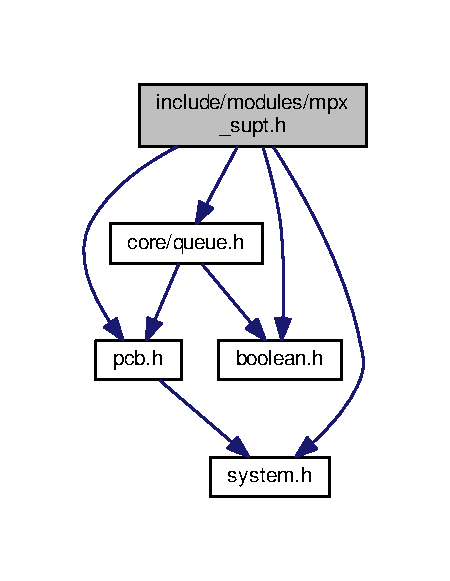
\includegraphics[width=216pt]{mpx__supt_8h__incl}
\end{center}
\end{figure}
This graph shows which files directly or indirectly include this file\+:\nopagebreak
\begin{figure}[H]
\begin{center}
\leavevmode
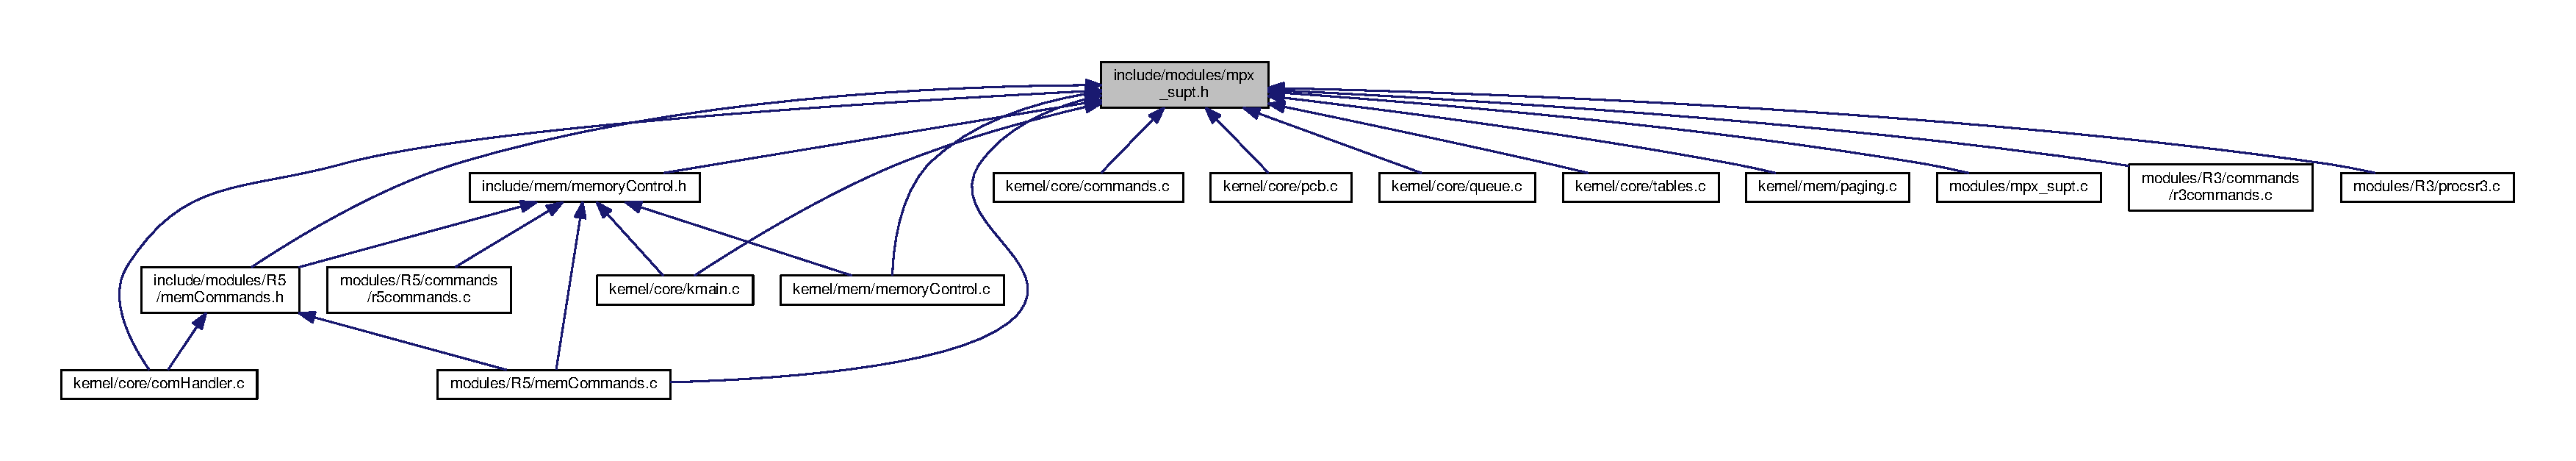
\includegraphics[width=350pt]{mpx__supt_8h__dep__incl}
\end{center}
\end{figure}
\subsection*{Data Structures}
\begin{DoxyCompactItemize}
\item 
struct \hyperlink{structparam}{param}
\item 
struct \hyperlink{structcontext}{context}
\end{DoxyCompactItemize}
\subsection*{Macros}
\begin{DoxyCompactItemize}
\item 
\#define \hyperlink{mpx__supt_8h_ad111e603bbebe5d87f6bc39264ce4733}{E\+X\+IT}~0
\item 
\#define \hyperlink{mpx__supt_8h_a9c21a7caee326d7803b94ae1952b27ca}{I\+D\+LE}~1
\item 
\#define \hyperlink{mpx__supt_8h_ada74e7db007a68e763f20c17f2985356}{R\+E\+AD}~2
\item 
\#define \hyperlink{mpx__supt_8h_aa10f470e996d0f51210d24f442d25e1e}{W\+R\+I\+TE}~3
\item 
\#define \hyperlink{mpx__supt_8h_a9d88621bfb79cb860b9ea2b5abb1c7f0}{M\+O\+D\+U\+L\+E\+\_\+\+R1}~0
\item 
\#define \hyperlink{mpx__supt_8h_a177f46669733cd706e9476485dfd961b}{M\+O\+D\+U\+L\+E\+\_\+\+R2}~1
\item 
\#define \hyperlink{mpx__supt_8h_afe0ac8d1ebddd519bed41c8d8e79fad0}{M\+O\+D\+U\+L\+E\+\_\+\+R3}~2
\item 
\#define \hyperlink{mpx__supt_8h_a05541487bcf6e840b918f0a6ef097024}{M\+O\+D\+U\+L\+E\+\_\+\+R4}~4
\item 
\#define \hyperlink{mpx__supt_8h_a68745bb3b58fd02dcee2cad3b2331def}{M\+O\+D\+U\+L\+E\+\_\+\+R5}~8
\end{DoxyCompactItemize}
\subsection*{Typedefs}
\begin{DoxyCompactItemize}
\item 
typedef struct \hyperlink{structcontext}{context} \hyperlink{mpx__supt_8h_a8a4c4daa317e8755642ca6d112f8aada}{context}
\end{DoxyCompactItemize}
\subsection*{Functions}
\begin{DoxyCompactItemize}
\item 
\hyperlink{system_8h_a757de76cafbcddaac0d1632902fe4cb8}{u32int} $\ast$ \hyperlink{mpx__supt_8h_aad8093682fcfe15c2669288f19d1c52c}{sys\+\_\+call} (\hyperlink{structcontext}{context} $\ast$registers)
\item 
void $\ast$ \hyperlink{mpx__supt_8h_ace6ee45c30e71865e6eb635200379db9}{memset} (void $\ast$s, int c, \hyperlink{system_8h_a7c94ea6f8948649f8d181ae55911eeaf}{size\+\_\+t} n)
\item 
int \hyperlink{mpx__supt_8h_afb6ff5e2e9bdde9d8971a497b6fe38ae}{sys\+\_\+req} (int op\+\_\+code)
\item 
void \hyperlink{mpx__supt_8h_a53332c6a3107a4feed6e2e79690a6ffa}{mpx\+\_\+init} (int cur\+\_\+mod)
\item 
void \hyperlink{mpx__supt_8h_a461113326a3bbb80ad5cca937558ca45}{sys\+\_\+set\+\_\+malloc} (void $\ast$($\ast$func)(int))
\item 
void \hyperlink{mpx__supt_8h_a339f3d08c4a16455cc58d20dfab4801f}{sys\+\_\+set\+\_\+free} (\hyperlink{boolean_8h_a7c6368b321bd9acd0149b030bb8275ed}{boolean}(func)(void $\ast$))
\item 
void $\ast$ \hyperlink{mpx__supt_8h_a61adad2abba0a3a225c2290b3de1fe93}{sys\+\_\+alloc\+\_\+mem} (\hyperlink{system_8h_a757de76cafbcddaac0d1632902fe4cb8}{u32int} size)
\item 
int \hyperlink{mpx__supt_8h_a950663d39dbb073c9dff9cf3b5d3392c}{sys\+\_\+free\+\_\+mem} (void $\ast$ptr)
\item 
void \hyperlink{mpx__supt_8h_a83abbeda22fc5e6c2b35523b64199c1c}{idle} ()
\item 
const char $\ast$ \hyperlink{mpx__supt_8h_ac82ba2233eada42af3611d09821b8906}{get\+C\+O\+P\+Name} ()
\end{DoxyCompactItemize}


\subsection{Macro Definition Documentation}
\index{mpx\+\_\+supt.\+h@{mpx\+\_\+supt.\+h}!E\+X\+IT@{E\+X\+IT}}
\index{E\+X\+IT@{E\+X\+IT}!mpx\+\_\+supt.\+h@{mpx\+\_\+supt.\+h}}
\subsubsection[{\texorpdfstring{E\+X\+IT}{EXIT}}]{\setlength{\rightskip}{0pt plus 5cm}\#define E\+X\+IT~0}\hypertarget{mpx__supt_8h_ad111e603bbebe5d87f6bc39264ce4733}{}\label{mpx__supt_8h_ad111e603bbebe5d87f6bc39264ce4733}
\index{mpx\+\_\+supt.\+h@{mpx\+\_\+supt.\+h}!I\+D\+LE@{I\+D\+LE}}
\index{I\+D\+LE@{I\+D\+LE}!mpx\+\_\+supt.\+h@{mpx\+\_\+supt.\+h}}
\subsubsection[{\texorpdfstring{I\+D\+LE}{IDLE}}]{\setlength{\rightskip}{0pt plus 5cm}\#define I\+D\+LE~1}\hypertarget{mpx__supt_8h_a9c21a7caee326d7803b94ae1952b27ca}{}\label{mpx__supt_8h_a9c21a7caee326d7803b94ae1952b27ca}
\index{mpx\+\_\+supt.\+h@{mpx\+\_\+supt.\+h}!M\+O\+D\+U\+L\+E\+\_\+\+R1@{M\+O\+D\+U\+L\+E\+\_\+\+R1}}
\index{M\+O\+D\+U\+L\+E\+\_\+\+R1@{M\+O\+D\+U\+L\+E\+\_\+\+R1}!mpx\+\_\+supt.\+h@{mpx\+\_\+supt.\+h}}
\subsubsection[{\texorpdfstring{M\+O\+D\+U\+L\+E\+\_\+\+R1}{MODULE_R1}}]{\setlength{\rightskip}{0pt plus 5cm}\#define M\+O\+D\+U\+L\+E\+\_\+\+R1~0}\hypertarget{mpx__supt_8h_a9d88621bfb79cb860b9ea2b5abb1c7f0}{}\label{mpx__supt_8h_a9d88621bfb79cb860b9ea2b5abb1c7f0}
\index{mpx\+\_\+supt.\+h@{mpx\+\_\+supt.\+h}!M\+O\+D\+U\+L\+E\+\_\+\+R2@{M\+O\+D\+U\+L\+E\+\_\+\+R2}}
\index{M\+O\+D\+U\+L\+E\+\_\+\+R2@{M\+O\+D\+U\+L\+E\+\_\+\+R2}!mpx\+\_\+supt.\+h@{mpx\+\_\+supt.\+h}}
\subsubsection[{\texorpdfstring{M\+O\+D\+U\+L\+E\+\_\+\+R2}{MODULE_R2}}]{\setlength{\rightskip}{0pt plus 5cm}\#define M\+O\+D\+U\+L\+E\+\_\+\+R2~1}\hypertarget{mpx__supt_8h_a177f46669733cd706e9476485dfd961b}{}\label{mpx__supt_8h_a177f46669733cd706e9476485dfd961b}
\index{mpx\+\_\+supt.\+h@{mpx\+\_\+supt.\+h}!M\+O\+D\+U\+L\+E\+\_\+\+R3@{M\+O\+D\+U\+L\+E\+\_\+\+R3}}
\index{M\+O\+D\+U\+L\+E\+\_\+\+R3@{M\+O\+D\+U\+L\+E\+\_\+\+R3}!mpx\+\_\+supt.\+h@{mpx\+\_\+supt.\+h}}
\subsubsection[{\texorpdfstring{M\+O\+D\+U\+L\+E\+\_\+\+R3}{MODULE_R3}}]{\setlength{\rightskip}{0pt plus 5cm}\#define M\+O\+D\+U\+L\+E\+\_\+\+R3~2}\hypertarget{mpx__supt_8h_afe0ac8d1ebddd519bed41c8d8e79fad0}{}\label{mpx__supt_8h_afe0ac8d1ebddd519bed41c8d8e79fad0}
\index{mpx\+\_\+supt.\+h@{mpx\+\_\+supt.\+h}!M\+O\+D\+U\+L\+E\+\_\+\+R4@{M\+O\+D\+U\+L\+E\+\_\+\+R4}}
\index{M\+O\+D\+U\+L\+E\+\_\+\+R4@{M\+O\+D\+U\+L\+E\+\_\+\+R4}!mpx\+\_\+supt.\+h@{mpx\+\_\+supt.\+h}}
\subsubsection[{\texorpdfstring{M\+O\+D\+U\+L\+E\+\_\+\+R4}{MODULE_R4}}]{\setlength{\rightskip}{0pt plus 5cm}\#define M\+O\+D\+U\+L\+E\+\_\+\+R4~4}\hypertarget{mpx__supt_8h_a05541487bcf6e840b918f0a6ef097024}{}\label{mpx__supt_8h_a05541487bcf6e840b918f0a6ef097024}
\index{mpx\+\_\+supt.\+h@{mpx\+\_\+supt.\+h}!M\+O\+D\+U\+L\+E\+\_\+\+R5@{M\+O\+D\+U\+L\+E\+\_\+\+R5}}
\index{M\+O\+D\+U\+L\+E\+\_\+\+R5@{M\+O\+D\+U\+L\+E\+\_\+\+R5}!mpx\+\_\+supt.\+h@{mpx\+\_\+supt.\+h}}
\subsubsection[{\texorpdfstring{M\+O\+D\+U\+L\+E\+\_\+\+R5}{MODULE_R5}}]{\setlength{\rightskip}{0pt plus 5cm}\#define M\+O\+D\+U\+L\+E\+\_\+\+R5~8}\hypertarget{mpx__supt_8h_a68745bb3b58fd02dcee2cad3b2331def}{}\label{mpx__supt_8h_a68745bb3b58fd02dcee2cad3b2331def}
\index{mpx\+\_\+supt.\+h@{mpx\+\_\+supt.\+h}!R\+E\+AD@{R\+E\+AD}}
\index{R\+E\+AD@{R\+E\+AD}!mpx\+\_\+supt.\+h@{mpx\+\_\+supt.\+h}}
\subsubsection[{\texorpdfstring{R\+E\+AD}{READ}}]{\setlength{\rightskip}{0pt plus 5cm}\#define R\+E\+AD~2}\hypertarget{mpx__supt_8h_ada74e7db007a68e763f20c17f2985356}{}\label{mpx__supt_8h_ada74e7db007a68e763f20c17f2985356}
\index{mpx\+\_\+supt.\+h@{mpx\+\_\+supt.\+h}!W\+R\+I\+TE@{W\+R\+I\+TE}}
\index{W\+R\+I\+TE@{W\+R\+I\+TE}!mpx\+\_\+supt.\+h@{mpx\+\_\+supt.\+h}}
\subsubsection[{\texorpdfstring{W\+R\+I\+TE}{WRITE}}]{\setlength{\rightskip}{0pt plus 5cm}\#define W\+R\+I\+TE~3}\hypertarget{mpx__supt_8h_aa10f470e996d0f51210d24f442d25e1e}{}\label{mpx__supt_8h_aa10f470e996d0f51210d24f442d25e1e}


\subsection{Typedef Documentation}
\index{mpx\+\_\+supt.\+h@{mpx\+\_\+supt.\+h}!context@{context}}
\index{context@{context}!mpx\+\_\+supt.\+h@{mpx\+\_\+supt.\+h}}
\subsubsection[{\texorpdfstring{context}{context}}]{\setlength{\rightskip}{0pt plus 5cm}typedef struct {\bf context}  {\bf context}}\hypertarget{mpx__supt_8h_a8a4c4daa317e8755642ca6d112f8aada}{}\label{mpx__supt_8h_a8a4c4daa317e8755642ca6d112f8aada}


\subsection{Function Documentation}
\index{mpx\+\_\+supt.\+h@{mpx\+\_\+supt.\+h}!get\+C\+O\+P\+Name@{get\+C\+O\+P\+Name}}
\index{get\+C\+O\+P\+Name@{get\+C\+O\+P\+Name}!mpx\+\_\+supt.\+h@{mpx\+\_\+supt.\+h}}
\subsubsection[{\texorpdfstring{get\+C\+O\+P\+Name()}{getCOPName()}}]{\setlength{\rightskip}{0pt plus 5cm}const char$\ast$ get\+C\+O\+P\+Name (
\begin{DoxyParamCaption}
{}
\end{DoxyParamCaption}
)}\hypertarget{mpx__supt_8h_ac82ba2233eada42af3611d09821b8906}{}\label{mpx__supt_8h_ac82ba2233eada42af3611d09821b8906}
Gets the name of the C\+OP

\begin{DoxyReturn}{Returns}
const char pointer name 
\end{DoxyReturn}
\index{mpx\+\_\+supt.\+h@{mpx\+\_\+supt.\+h}!idle@{idle}}
\index{idle@{idle}!mpx\+\_\+supt.\+h@{mpx\+\_\+supt.\+h}}
\subsubsection[{\texorpdfstring{idle()}{idle()}}]{\setlength{\rightskip}{0pt plus 5cm}void idle (
\begin{DoxyParamCaption}
{}
\end{DoxyParamCaption}
)}\hypertarget{mpx__supt_8h_a83abbeda22fc5e6c2b35523b64199c1c}{}\label{mpx__supt_8h_a83abbeda22fc5e6c2b35523b64199c1c}
The idle process \index{mpx\+\_\+supt.\+h@{mpx\+\_\+supt.\+h}!memset@{memset}}
\index{memset@{memset}!mpx\+\_\+supt.\+h@{mpx\+\_\+supt.\+h}}
\subsubsection[{\texorpdfstring{memset(void $\ast$s, int c, size\+\_\+t n)}{memset(void *s, int c, size_t n)}}]{\setlength{\rightskip}{0pt plus 5cm}void$\ast$ memset (
\begin{DoxyParamCaption}
\item[{void $\ast$}]{s, }
\item[{int}]{c, }
\item[{{\bf size\+\_\+t}}]{n}
\end{DoxyParamCaption}
)}\hypertarget{mpx__supt_8h_ace6ee45c30e71865e6eb635200379db9}{}\label{mpx__supt_8h_ace6ee45c30e71865e6eb635200379db9}
Set a region of memory


\begin{DoxyParams}{Parameters}
{\em s} & Destination \\
\hline
{\em c} & Byte to write \\
\hline
{\em n} & Count \\
\hline
\end{DoxyParams}
\begin{DoxyReturn}{Returns}
s 
\end{DoxyReturn}
\index{mpx\+\_\+supt.\+h@{mpx\+\_\+supt.\+h}!mpx\+\_\+init@{mpx\+\_\+init}}
\index{mpx\+\_\+init@{mpx\+\_\+init}!mpx\+\_\+supt.\+h@{mpx\+\_\+supt.\+h}}
\subsubsection[{\texorpdfstring{mpx\+\_\+init(int cur\+\_\+mod)}{mpx_init(int cur_mod)}}]{\setlength{\rightskip}{0pt plus 5cm}void mpx\+\_\+init (
\begin{DoxyParamCaption}
\item[{int}]{cur\+\_\+mod}
\end{DoxyParamCaption}
)}\hypertarget{mpx__supt_8h_a53332c6a3107a4feed6e2e79690a6ffa}{}\label{mpx__supt_8h_a53332c6a3107a4feed6e2e79690a6ffa}
Initialize M\+PX support software


\begin{DoxyParams}{Parameters}
{\em cur\+\_\+mod} & (symbolic constants M\+O\+D\+U\+L\+E\+\_\+\+R1, M\+O\+D\+U\+L\+E\+\_\+\+R2, etc) \\
\hline
\end{DoxyParams}
\index{mpx\+\_\+supt.\+h@{mpx\+\_\+supt.\+h}!sys\+\_\+alloc\+\_\+mem@{sys\+\_\+alloc\+\_\+mem}}
\index{sys\+\_\+alloc\+\_\+mem@{sys\+\_\+alloc\+\_\+mem}!mpx\+\_\+supt.\+h@{mpx\+\_\+supt.\+h}}
\subsubsection[{\texorpdfstring{sys\+\_\+alloc\+\_\+mem(u32int size)}{sys_alloc_mem(u32int size)}}]{\setlength{\rightskip}{0pt plus 5cm}void$\ast$ sys\+\_\+alloc\+\_\+mem (
\begin{DoxyParamCaption}
\item[{{\bf u32int}}]{size}
\end{DoxyParamCaption}
)}\hypertarget{mpx__supt_8h_a61adad2abba0a3a225c2290b3de1fe93}{}\label{mpx__supt_8h_a61adad2abba0a3a225c2290b3de1fe93}
Allocates a block of memory (similar to malloc)


\begin{DoxyParams}{Parameters}
{\em size} & Number of bytes to allocate \\
\hline
\end{DoxyParams}
\begin{DoxyReturn}{Returns}
The allocated memory 
\end{DoxyReturn}
\index{mpx\+\_\+supt.\+h@{mpx\+\_\+supt.\+h}!sys\+\_\+call@{sys\+\_\+call}}
\index{sys\+\_\+call@{sys\+\_\+call}!mpx\+\_\+supt.\+h@{mpx\+\_\+supt.\+h}}
\subsubsection[{\texorpdfstring{sys\+\_\+call(context $\ast$registers)}{sys_call(context *registers)}}]{\setlength{\rightskip}{0pt plus 5cm}{\bf u32int}$\ast$ sys\+\_\+call (
\begin{DoxyParamCaption}
\item[{{\bf context} $\ast$}]{registers}
\end{DoxyParamCaption}
)}\hypertarget{mpx__supt_8h_aad8093682fcfe15c2669288f19d1c52c}{}\label{mpx__supt_8h_aad8093682fcfe15c2669288f19d1c52c}
Changes the currently running process to that of the next ready process


\begin{DoxyParams}{Parameters}
{\em registers} & -\/ copy of register values \\
\hline
\end{DoxyParams}
\begin{DoxyReturn}{Returns}
u32int position of stack\+Top 
\end{DoxyReturn}
\index{mpx\+\_\+supt.\+h@{mpx\+\_\+supt.\+h}!sys\+\_\+free\+\_\+mem@{sys\+\_\+free\+\_\+mem}}
\index{sys\+\_\+free\+\_\+mem@{sys\+\_\+free\+\_\+mem}!mpx\+\_\+supt.\+h@{mpx\+\_\+supt.\+h}}
\subsubsection[{\texorpdfstring{sys\+\_\+free\+\_\+mem(void $\ast$ptr)}{sys_free_mem(void *ptr)}}]{\setlength{\rightskip}{0pt plus 5cm}int sys\+\_\+free\+\_\+mem (
\begin{DoxyParamCaption}
\item[{void $\ast$}]{ptr}
\end{DoxyParamCaption}
)}\hypertarget{mpx__supt_8h_a950663d39dbb073c9dff9cf3b5d3392c}{}\label{mpx__supt_8h_a950663d39dbb073c9dff9cf3b5d3392c}
Frees memory


\begin{DoxyParams}{Parameters}
{\em ptr} & Pointer to the block of memory to free \\
\hline
\end{DoxyParams}
\begin{DoxyReturn}{Returns}

\end{DoxyReturn}
\index{mpx\+\_\+supt.\+h@{mpx\+\_\+supt.\+h}!sys\+\_\+req@{sys\+\_\+req}}
\index{sys\+\_\+req@{sys\+\_\+req}!mpx\+\_\+supt.\+h@{mpx\+\_\+supt.\+h}}
\subsubsection[{\texorpdfstring{sys\+\_\+req(int op\+\_\+code)}{sys_req(int op_code)}}]{\setlength{\rightskip}{0pt plus 5cm}int sys\+\_\+req (
\begin{DoxyParamCaption}
\item[{int}]{op\+\_\+code}
\end{DoxyParamCaption}
)}\hypertarget{mpx__supt_8h_afb6ff5e2e9bdde9d8971a497b6fe38ae}{}\label{mpx__supt_8h_afb6ff5e2e9bdde9d8971a497b6fe38ae}
Generates interrupt 60H


\begin{DoxyParams}{Parameters}
{\em op\+\_\+code} & (I\+D\+LE) \\
\hline
\end{DoxyParams}
\begin{DoxyReturn}{Returns}
0 
\end{DoxyReturn}
\index{mpx\+\_\+supt.\+h@{mpx\+\_\+supt.\+h}!sys\+\_\+set\+\_\+free@{sys\+\_\+set\+\_\+free}}
\index{sys\+\_\+set\+\_\+free@{sys\+\_\+set\+\_\+free}!mpx\+\_\+supt.\+h@{mpx\+\_\+supt.\+h}}
\subsubsection[{\texorpdfstring{sys\+\_\+set\+\_\+free(boolean(func)(void $\ast$))}{sys_set_free(boolean(func)(void *))}}]{\setlength{\rightskip}{0pt plus 5cm}void sys\+\_\+set\+\_\+free (
\begin{DoxyParamCaption}
\item[{{\bf boolean}(func)(void $\ast$)}]{}
\end{DoxyParamCaption}
)}\hypertarget{mpx__supt_8h_a339f3d08c4a16455cc58d20dfab4801f}{}\label{mpx__supt_8h_a339f3d08c4a16455cc58d20dfab4801f}
Sets the memory free function for sys\+\_\+free\+\_\+mem


\begin{DoxyParams}{Parameters}
{\em func} & Function pointer to the memory free-\/er \\
\hline
\end{DoxyParams}
\index{mpx\+\_\+supt.\+h@{mpx\+\_\+supt.\+h}!sys\+\_\+set\+\_\+malloc@{sys\+\_\+set\+\_\+malloc}}
\index{sys\+\_\+set\+\_\+malloc@{sys\+\_\+set\+\_\+malloc}!mpx\+\_\+supt.\+h@{mpx\+\_\+supt.\+h}}
\subsubsection[{\texorpdfstring{sys\+\_\+set\+\_\+malloc(void $\ast$($\ast$func)(int))}{sys_set_malloc(void *(*func)(int))}}]{\setlength{\rightskip}{0pt plus 5cm}void sys\+\_\+set\+\_\+malloc (
\begin{DoxyParamCaption}
\item[{void $\ast$($\ast$)(int)}]{func}
\end{DoxyParamCaption}
)}\hypertarget{mpx__supt_8h_a461113326a3bbb80ad5cca937558ca45}{}\label{mpx__supt_8h_a461113326a3bbb80ad5cca937558ca45}
Sets the memory allocation function for sys\+\_\+alloc\+\_\+mem


\begin{DoxyParams}{Parameters}
{\em func} & Function pointer to the memory allocator \\
\hline
\end{DoxyParams}

\hypertarget{help__temp_8h}{}\section{include/modules/\+R2/commands/help\+\_\+temp.h File Reference}
\label{help__temp_8h}\index{include/modules/\+R2/commands/help\+\_\+temp.\+h@{include/modules/\+R2/commands/help\+\_\+temp.\+h}}
This graph shows which files directly or indirectly include this file\+:\nopagebreak
\begin{figure}[H]
\begin{center}
\leavevmode
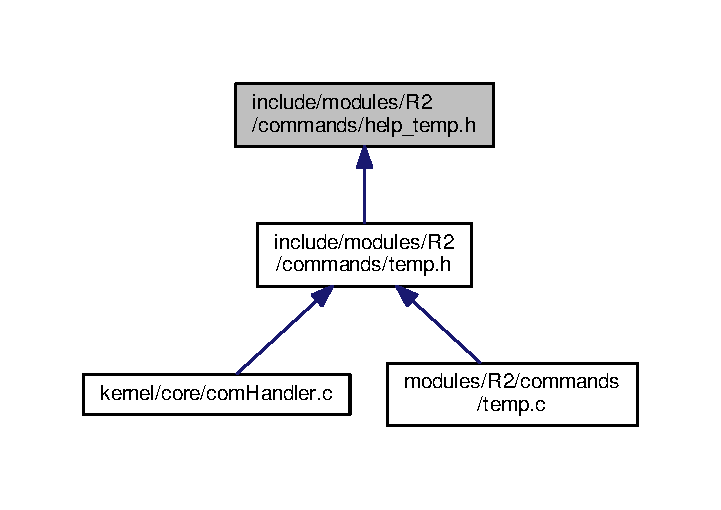
\includegraphics[width=346pt]{help__temp_8h__dep__incl}
\end{center}
\end{figure}
\subsection*{Macros}
\begin{DoxyCompactItemize}
\item 
\#define \hyperlink{help__temp_8h_a14a992a53cf97e2680d36d59c040af00}{H\+E\+L\+P\+\_\+\+R2\+\_\+\+C\+O\+M\+M\+A\+N\+D\+\_\+\+C\+P\+CB}
\item 
\#define \hyperlink{help__temp_8h_af0afce80946a346875137e9ccbf02018}{H\+E\+L\+P\+\_\+\+R2\+\_\+\+C\+O\+M\+M\+A\+N\+D\+\_\+\+D\+P\+CB}
\item 
\#define \hyperlink{help__temp_8h_a0ad95dbd36602ae2b1ae6fab25f77218}{H\+E\+L\+P\+\_\+\+R2\+\_\+\+C\+O\+M\+M\+A\+N\+D\+\_\+\+B\+P\+CB}
\item 
\#define \hyperlink{help__temp_8h_a381cd747906cd1e579e4ee8886705e81}{H\+E\+L\+P\+\_\+\+R2\+\_\+\+C\+O\+M\+M\+A\+N\+D\+\_\+\+U\+P\+CB}
\end{DoxyCompactItemize}


\subsection{Macro Definition Documentation}
\index{help\+\_\+temp.\+h@{help\+\_\+temp.\+h}!H\+E\+L\+P\+\_\+\+R2\+\_\+\+C\+O\+M\+M\+A\+N\+D\+\_\+\+B\+P\+CB@{H\+E\+L\+P\+\_\+\+R2\+\_\+\+C\+O\+M\+M\+A\+N\+D\+\_\+\+B\+P\+CB}}
\index{H\+E\+L\+P\+\_\+\+R2\+\_\+\+C\+O\+M\+M\+A\+N\+D\+\_\+\+B\+P\+CB@{H\+E\+L\+P\+\_\+\+R2\+\_\+\+C\+O\+M\+M\+A\+N\+D\+\_\+\+B\+P\+CB}!help\+\_\+temp.\+h@{help\+\_\+temp.\+h}}
\subsubsection[{\texorpdfstring{H\+E\+L\+P\+\_\+\+R2\+\_\+\+C\+O\+M\+M\+A\+N\+D\+\_\+\+B\+P\+CB}{HELP_R2_COMMAND_BPCB}}]{\setlength{\rightskip}{0pt plus 5cm}\#define H\+E\+L\+P\+\_\+\+R2\+\_\+\+C\+O\+M\+M\+A\+N\+D\+\_\+\+B\+P\+CB}\hypertarget{help__temp_8h_a0ad95dbd36602ae2b1ae6fab25f77218}{}\label{help__temp_8h_a0ad95dbd36602ae2b1ae6fab25f77218}
{\bfseries Value\+:}
\begin{DoxyCode}
((\textcolor{keyword}{const} \textcolor{keywordtype}{char}*) \(\backslash\)
    \textcolor{stringliteral}{"Places a PCB into the blocked state and reinserts it into the appropriate queue.\(\backslash\)n"}\(\backslash\)
    \textcolor{stringliteral}{"\(\backslash\)n"}\(\backslash\)
    \textcolor{stringliteral}{"Note: This command will be removed in module R3/R4\(\backslash\)n"}\(\backslash\)
    \textcolor{stringliteral}{"\(\backslash\)n"}\(\backslash\)
    \textcolor{stringliteral}{"Usage: bpcb name\(\backslash\)n"}\(\backslash\)
    \textcolor{stringliteral}{"\(\backslash\)n"}\(\backslash\)
    \textcolor{stringliteral}{"Args:\(\backslash\)n"}\(\backslash\)
    \textcolor{stringliteral}{"    name - The Process Name to place into the blocked state (must exist)"})
\end{DoxyCode}
\index{help\+\_\+temp.\+h@{help\+\_\+temp.\+h}!H\+E\+L\+P\+\_\+\+R2\+\_\+\+C\+O\+M\+M\+A\+N\+D\+\_\+\+C\+P\+CB@{H\+E\+L\+P\+\_\+\+R2\+\_\+\+C\+O\+M\+M\+A\+N\+D\+\_\+\+C\+P\+CB}}
\index{H\+E\+L\+P\+\_\+\+R2\+\_\+\+C\+O\+M\+M\+A\+N\+D\+\_\+\+C\+P\+CB@{H\+E\+L\+P\+\_\+\+R2\+\_\+\+C\+O\+M\+M\+A\+N\+D\+\_\+\+C\+P\+CB}!help\+\_\+temp.\+h@{help\+\_\+temp.\+h}}
\subsubsection[{\texorpdfstring{H\+E\+L\+P\+\_\+\+R2\+\_\+\+C\+O\+M\+M\+A\+N\+D\+\_\+\+C\+P\+CB}{HELP_R2_COMMAND_CPCB}}]{\setlength{\rightskip}{0pt plus 5cm}\#define H\+E\+L\+P\+\_\+\+R2\+\_\+\+C\+O\+M\+M\+A\+N\+D\+\_\+\+C\+P\+CB}\hypertarget{help__temp_8h_a14a992a53cf97e2680d36d59c040af00}{}\label{help__temp_8h_a14a992a53cf97e2680d36d59c040af00}
{\bfseries Value\+:}
\begin{DoxyCode}
((\textcolor{keyword}{const} \textcolor{keywordtype}{char}*) \(\backslash\)
    \textcolor{stringliteral}{"Creates a PCB and inserts it into the appropriate queue.\(\backslash\)n"}\(\backslash\)
    \textcolor{stringliteral}{"\(\backslash\)n"}\(\backslash\)
    \textcolor{stringliteral}{"Note: This command will be removed in module R3/R4\(\backslash\)n"}\(\backslash\)
    \textcolor{stringliteral}{"\(\backslash\)n"}\(\backslash\)
    \textcolor{stringliteral}{"Usage: cpcb name class priority\(\backslash\)n"}\(\backslash\)
    \textcolor{stringliteral}{"\(\backslash\)n"}\(\backslash\)
    \textcolor{stringliteral}{"Args:\(\backslash\)n"}\(\backslash\)
    \textcolor{stringliteral}{"    name - The Process Name (must be unique)\(\backslash\)n"}\(\backslash\)
    \textcolor{stringliteral}{"    class - The Process Class (either 0 (system) or 1 (application))\(\backslash\)n"}\(\backslash\)
    \textcolor{stringliteral}{"    priority - The Process Priority (number between 0 and 9)"})
\end{DoxyCode}
\index{help\+\_\+temp.\+h@{help\+\_\+temp.\+h}!H\+E\+L\+P\+\_\+\+R2\+\_\+\+C\+O\+M\+M\+A\+N\+D\+\_\+\+D\+P\+CB@{H\+E\+L\+P\+\_\+\+R2\+\_\+\+C\+O\+M\+M\+A\+N\+D\+\_\+\+D\+P\+CB}}
\index{H\+E\+L\+P\+\_\+\+R2\+\_\+\+C\+O\+M\+M\+A\+N\+D\+\_\+\+D\+P\+CB@{H\+E\+L\+P\+\_\+\+R2\+\_\+\+C\+O\+M\+M\+A\+N\+D\+\_\+\+D\+P\+CB}!help\+\_\+temp.\+h@{help\+\_\+temp.\+h}}
\subsubsection[{\texorpdfstring{H\+E\+L\+P\+\_\+\+R2\+\_\+\+C\+O\+M\+M\+A\+N\+D\+\_\+\+D\+P\+CB}{HELP_R2_COMMAND_DPCB}}]{\setlength{\rightskip}{0pt plus 5cm}\#define H\+E\+L\+P\+\_\+\+R2\+\_\+\+C\+O\+M\+M\+A\+N\+D\+\_\+\+D\+P\+CB}\hypertarget{help__temp_8h_af0afce80946a346875137e9ccbf02018}{}\label{help__temp_8h_af0afce80946a346875137e9ccbf02018}
{\bfseries Value\+:}
\begin{DoxyCode}
((\textcolor{keyword}{const} \textcolor{keywordtype}{char}*) \(\backslash\)
    \textcolor{stringliteral}{"Removes a PCB from the appropriate queue and then frees all associated memory.\(\backslash\)n"}\(\backslash\)
    \textcolor{stringliteral}{"\(\backslash\)n"}\(\backslash\)
    \textcolor{stringliteral}{"Note: This command will be removed in module R3/R4\(\backslash\)n"}\(\backslash\)
    \textcolor{stringliteral}{"\(\backslash\)n"}\(\backslash\)
    \textcolor{stringliteral}{"Usage: dpcb name\(\backslash\)n"}\(\backslash\)
    \textcolor{stringliteral}{"\(\backslash\)n"}\(\backslash\)
    \textcolor{stringliteral}{"Args:\(\backslash\)n"}\(\backslash\)
    \textcolor{stringliteral}{"    name - The Process Name to remove (must exist)"})
\end{DoxyCode}
\index{help\+\_\+temp.\+h@{help\+\_\+temp.\+h}!H\+E\+L\+P\+\_\+\+R2\+\_\+\+C\+O\+M\+M\+A\+N\+D\+\_\+\+U\+P\+CB@{H\+E\+L\+P\+\_\+\+R2\+\_\+\+C\+O\+M\+M\+A\+N\+D\+\_\+\+U\+P\+CB}}
\index{H\+E\+L\+P\+\_\+\+R2\+\_\+\+C\+O\+M\+M\+A\+N\+D\+\_\+\+U\+P\+CB@{H\+E\+L\+P\+\_\+\+R2\+\_\+\+C\+O\+M\+M\+A\+N\+D\+\_\+\+U\+P\+CB}!help\+\_\+temp.\+h@{help\+\_\+temp.\+h}}
\subsubsection[{\texorpdfstring{H\+E\+L\+P\+\_\+\+R2\+\_\+\+C\+O\+M\+M\+A\+N\+D\+\_\+\+U\+P\+CB}{HELP_R2_COMMAND_UPCB}}]{\setlength{\rightskip}{0pt plus 5cm}\#define H\+E\+L\+P\+\_\+\+R2\+\_\+\+C\+O\+M\+M\+A\+N\+D\+\_\+\+U\+P\+CB}\hypertarget{help__temp_8h_a381cd747906cd1e579e4ee8886705e81}{}\label{help__temp_8h_a381cd747906cd1e579e4ee8886705e81}
{\bfseries Value\+:}
\begin{DoxyCode}
((\textcolor{keyword}{const} \textcolor{keywordtype}{char}*) \(\backslash\)
    \textcolor{stringliteral}{"Places a PCB into the unblocked state and reinserts it into the appropriate queue.\(\backslash\)n"}\(\backslash\)
    \textcolor{stringliteral}{"\(\backslash\)n"}\(\backslash\)
    \textcolor{stringliteral}{"Note: This command will be removed in module R3/R4\(\backslash\)n"}\(\backslash\)
    \textcolor{stringliteral}{"\(\backslash\)n"}\(\backslash\)
    \textcolor{stringliteral}{"Usage: upcb name\(\backslash\)n"}\(\backslash\)
    \textcolor{stringliteral}{"\(\backslash\)n"}\(\backslash\)
    \textcolor{stringliteral}{"Args:\(\backslash\)n"}\(\backslash\)
    \textcolor{stringliteral}{"    name - The Process Name to place into the unblocked state (must exist)"})
\end{DoxyCode}

\hypertarget{perm_8h}{}\section{include/modules/\+R2/commands/perm.h File Reference}
\label{perm_8h}\index{include/modules/\+R2/commands/perm.\+h@{include/modules/\+R2/commands/perm.\+h}}
{\ttfamily \#include \char`\"{}help.\+h\char`\"{}}\\*
{\ttfamily \#include \char`\"{}status.\+h\char`\"{}}\\*
Include dependency graph for perm.\+h\+:\nopagebreak
\begin{figure}[H]
\begin{center}
\leavevmode
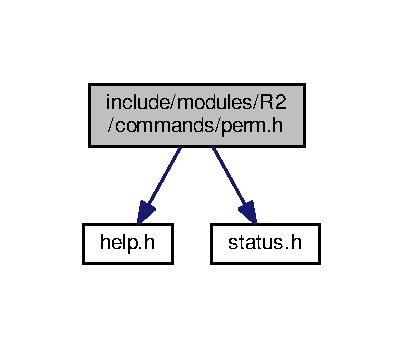
\includegraphics[width=194pt]{perm_8h__incl}
\end{center}
\end{figure}
This graph shows which files directly or indirectly include this file\+:\nopagebreak
\begin{figure}[H]
\begin{center}
\leavevmode
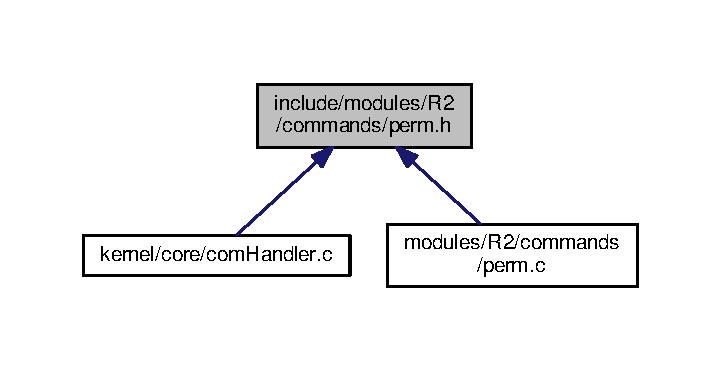
\includegraphics[width=346pt]{perm_8h__dep__incl}
\end{center}
\end{figure}
\subsection*{Functions}
\begin{DoxyCompactItemize}
\item 
void \hyperlink{perm_8h_a81a1071e7a98eaced2f1b4a418df87cb}{register\+R2\+Perm\+Commands} ()
\item 
const char $\ast$ \hyperlink{perm_8h_aeb3891b8b6fa80f3307b8c83bf8c6178}{suspend\+Pcb} (char $\ast$$\ast$args, int num\+Args)
\item 
const char $\ast$ \hyperlink{perm_8h_a3107aea4894efdf8a23240ee68869822}{resume\+Pcb} (char $\ast$$\ast$args, int num\+Args)
\item 
const char $\ast$ \hyperlink{perm_8h_a4aca0351fa322b227ff3114f0c7b8a04}{set\+Priority\+Pcb} (char $\ast$$\ast$args, int num\+Args)
\item 
const char $\ast$ \hyperlink{perm_8h_a4ece86bfd9ed049b2779020662b8b022}{show\+Pcb\+Info} (char $\ast$$\ast$args, int num\+Args)
\end{DoxyCompactItemize}


\subsection{Function Documentation}
\index{perm.\+h@{perm.\+h}!register\+R2\+Perm\+Commands@{register\+R2\+Perm\+Commands}}
\index{register\+R2\+Perm\+Commands@{register\+R2\+Perm\+Commands}!perm.\+h@{perm.\+h}}
\subsubsection[{\texorpdfstring{register\+R2\+Perm\+Commands()}{registerR2PermCommands()}}]{\setlength{\rightskip}{0pt plus 5cm}void register\+R2\+Perm\+Commands (
\begin{DoxyParamCaption}
{}
\end{DoxyParamCaption}
)}\hypertarget{perm_8h_a81a1071e7a98eaced2f1b4a418df87cb}{}\label{perm_8h_a81a1071e7a98eaced2f1b4a418df87cb}
Registers the permanent commands in the command handler \index{perm.\+h@{perm.\+h}!resume\+Pcb@{resume\+Pcb}}
\index{resume\+Pcb@{resume\+Pcb}!perm.\+h@{perm.\+h}}
\subsubsection[{\texorpdfstring{resume\+Pcb(char $\ast$$\ast$args, int num\+Args)}{resumePcb(char **args, int numArgs)}}]{\setlength{\rightskip}{0pt plus 5cm}const char$\ast$ resume\+Pcb (
\begin{DoxyParamCaption}
\item[{char $\ast$$\ast$}]{args, }
\item[{int}]{num\+Args}
\end{DoxyParamCaption}
)}\hypertarget{perm_8h_a3107aea4894efdf8a23240ee68869822}{}\label{perm_8h_a3107aea4894efdf8a23240ee68869822}
Places a P\+CB into the not suspended state and reinserts it into the appropriate queue.

Usage\+: rpcb name

Args\+: name -\/ The name of the process to resume (must exist)


\begin{DoxyParams}{Parameters}
{\em args} & The arguments to pass to the function \\
\hline
{\em num\+Args} & The number of arguments \\
\hline
\end{DoxyParams}
\begin{DoxyReturn}{Returns}
A status message indicating success/failure
\end{DoxyReturn}
Places a P\+CB into the not suspended state and reinserts it into the appropriate queue.

Usage\+: rpcb name

Args\+: name -\/ The name of the process to resume (must exist) --all -\/ Resumes all processes


\begin{DoxyParams}{Parameters}
{\em args} & The arguments to pass to the function \\
\hline
{\em num\+Args} & The number of arguments \\
\hline
\end{DoxyParams}
\begin{DoxyReturn}{Returns}
A status message indicating success/failure 
\end{DoxyReturn}
\index{perm.\+h@{perm.\+h}!set\+Priority\+Pcb@{set\+Priority\+Pcb}}
\index{set\+Priority\+Pcb@{set\+Priority\+Pcb}!perm.\+h@{perm.\+h}}
\subsubsection[{\texorpdfstring{set\+Priority\+Pcb(char $\ast$$\ast$args, int num\+Args)}{setPriorityPcb(char **args, int numArgs)}}]{\setlength{\rightskip}{0pt plus 5cm}const char$\ast$ set\+Priority\+Pcb (
\begin{DoxyParamCaption}
\item[{char $\ast$$\ast$}]{args, }
\item[{int}]{num\+Args}
\end{DoxyParamCaption}
)}\hypertarget{perm_8h_a4aca0351fa322b227ff3114f0c7b8a04}{}\label{perm_8h_a4aca0351fa322b227ff3114f0c7b8a04}
Sets a P\+CB\textquotesingle{}s priority and reinserts the process into the correct place in the correct queue.

Usage\+: ppcb name priority

Args\+: name -\/ The name of the process to set the priority on (must exist) priority -\/ The new priority (between 0 and 9)


\begin{DoxyParams}{Parameters}
{\em args} & The arguments to pass to the function \\
\hline
{\em num\+Args} & The number of arguments \\
\hline
\end{DoxyParams}
\begin{DoxyReturn}{Returns}
A status message indicating success/failure 
\end{DoxyReturn}
\index{perm.\+h@{perm.\+h}!show\+Pcb\+Info@{show\+Pcb\+Info}}
\index{show\+Pcb\+Info@{show\+Pcb\+Info}!perm.\+h@{perm.\+h}}
\subsubsection[{\texorpdfstring{show\+Pcb\+Info(char $\ast$$\ast$args, int num\+Args)}{showPcbInfo(char **args, int numArgs)}}]{\setlength{\rightskip}{0pt plus 5cm}const char$\ast$ show\+Pcb\+Info (
\begin{DoxyParamCaption}
\item[{char $\ast$$\ast$}]{args, }
\item[{int}]{num\+Args}
\end{DoxyParamCaption}
)}\hypertarget{perm_8h_a4ece86bfd9ed049b2779020662b8b022}{}\label{perm_8h_a4ece86bfd9ed049b2779020662b8b022}
Displays the following information for the specified P\+C\+Bs\+: Process Name\+: Class\+: State\+: Suspended Status\+: Priority\+:

Usage\+: showpcb \mbox{[}--all\mbox{]} \mbox{[}--ready\mbox{]} \mbox{[}--blocked\mbox{]} \mbox{[}--name pcb\+Name\mbox{]} (at least 1 must be specified)

Args\+: \mbox{[}no args\mbox{]} -\/ Shows the help for this command --all -\/ Displays information for all P\+C\+Bs --ready -\/ Displays information for ready P\+C\+Bs --blocked -\/ Displays information for blocked P\+C\+Bs --suspended -\/ Displays information for suspended P\+C\+Bs --name -\/ Displays information for the specified P\+CB (can be used multiple times)


\begin{DoxyParams}{Parameters}
{\em args} & The arguments to pass to the function \\
\hline
{\em num\+Args} & The number of arguments \\
\hline
\end{DoxyParams}
\begin{DoxyReturn}{Returns}
A status message indicating success/failure
\end{DoxyReturn}
Displays the following information for the specified P\+C\+Bs\+: Process Name\+: Class\+: State\+: Suspended Status\+: Priority\+:

Usage\+: showpcb \mbox{[}--all\mbox{]} \mbox{[}--ready\mbox{]} \mbox{[}--blocked\mbox{]} \mbox{[}--suspended\mbox{]} \mbox{[}--name pcb\+Name\mbox{]}

Args\+: \mbox{[}no args\mbox{]} -\/ Shows the help for this command --all -\/ Displays information for all P\+C\+Bs --ready -\/ Displays information for ready P\+C\+Bs --blocked -\/ Displays information for blocked P\+C\+Bs --suspended -\/ Displays information for suspended P\+C\+Bs --name -\/ Displays information for the specified P\+CB


\begin{DoxyParams}{Parameters}
{\em args} & The arguments to pass to the function \\
\hline
{\em num\+Args} & The number of arguments \\
\hline
\end{DoxyParams}
\begin{DoxyReturn}{Returns}
A status message indicating success/failure 
\end{DoxyReturn}
\index{perm.\+h@{perm.\+h}!suspend\+Pcb@{suspend\+Pcb}}
\index{suspend\+Pcb@{suspend\+Pcb}!perm.\+h@{perm.\+h}}
\subsubsection[{\texorpdfstring{suspend\+Pcb(char $\ast$$\ast$args, int num\+Args)}{suspendPcb(char **args, int numArgs)}}]{\setlength{\rightskip}{0pt plus 5cm}const char$\ast$ suspend\+Pcb (
\begin{DoxyParamCaption}
\item[{char $\ast$$\ast$}]{args, }
\item[{int}]{num\+Args}
\end{DoxyParamCaption}
)}\hypertarget{perm_8h_aeb3891b8b6fa80f3307b8c83bf8c6178}{}\label{perm_8h_aeb3891b8b6fa80f3307b8c83bf8c6178}
Places a P\+CB into the suspended state and reinserts it into the appropriate queue.

Usage\+: spcb name

Args\+: name -\/ The name of the process to suspend (must exist) --all -\/ Resumes all processes


\begin{DoxyParams}{Parameters}
{\em args} & The arguments to pass to the function \\
\hline
{\em num\+Args} & The number of arguments \\
\hline
\end{DoxyParams}
\begin{DoxyReturn}{Returns}
A status message indicating success/failure 
\end{DoxyReturn}

\hypertarget{status_8h}{}\section{include/modules/\+R2/commands/status.h File Reference}
\label{status_8h}\index{include/modules/\+R2/commands/status.\+h@{include/modules/\+R2/commands/status.\+h}}
This graph shows which files directly or indirectly include this file\+:\nopagebreak
\begin{figure}[H]
\begin{center}
\leavevmode
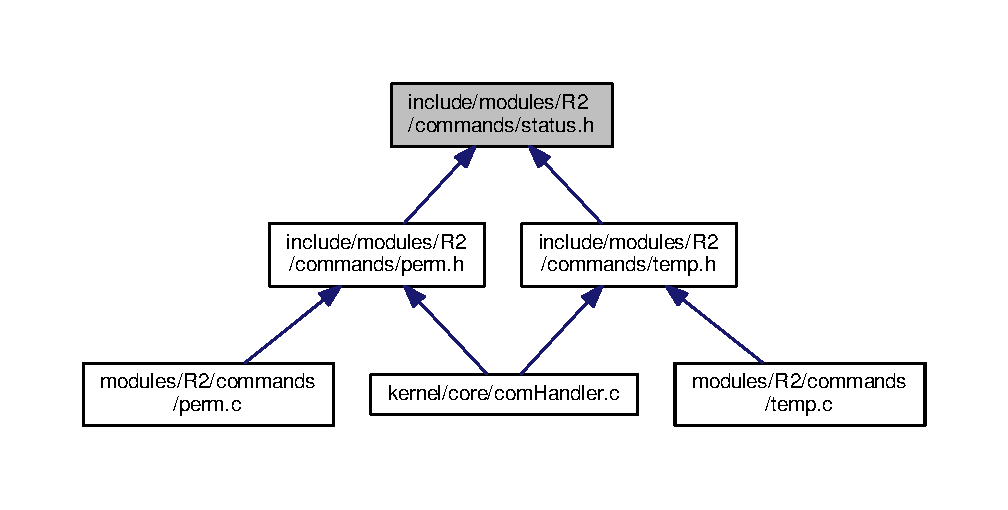
\includegraphics[width=350pt]{status_8h__dep__incl}
\end{center}
\end{figure}
\subsection*{Macros}
\begin{DoxyCompactItemize}
\item 
\#define \hyperlink{status_8h_a66a0164c254daac42696e0cb6719a64e}{U\+N\+K\+N\+O\+W\+N\+\_\+\+P\+C\+B\+\_\+\+N\+A\+ME}~((const char$\ast$) \char`\"{}Unknown P\+CB name.\char`\"{})
\item 
\#define \hyperlink{status_8h_adbb3bc7034dadbed6f4ae1e6f574f9be}{S\+U\+S\+P\+E\+N\+D\+\_\+\+P\+C\+B\+\_\+\+S\+U\+C\+C\+E\+SS}~((const char$\ast$) \char`\"{}Process suspended.\char`\"{})
\item 
\#define \hyperlink{status_8h_abbe82b179368fce3b4c1746fe5c5a295}{R\+E\+S\+U\+M\+E\+\_\+\+P\+C\+B\+\_\+\+S\+U\+C\+C\+E\+SS}~((const char$\ast$) \char`\"{}Process resumed.\char`\"{})
\item 
\#define \hyperlink{status_8h_a15f305673049d2a01548d4f232eaf9ac}{R\+E\+S\+U\+M\+E\+\_\+\+P\+C\+B\+S\+\_\+\+S\+U\+C\+C\+E\+SS}~((const char$\ast$) \char`\"{}All processes resumed.\char`\"{})
\item 
\#define \hyperlink{status_8h_ad27ebfa85f071ed58a9504a1e52af217}{U\+P\+D\+A\+T\+E\+\_\+\+P\+R\+I\+O\+R\+I\+T\+Y\+\_\+\+S\+U\+C\+C\+E\+SS}~((const char$\ast$) \char`\"{}Priority updated.\char`\"{})
\end{DoxyCompactItemize}


\subsection{Macro Definition Documentation}
\index{status.\+h@{status.\+h}!R\+E\+S\+U\+M\+E\+\_\+\+P\+C\+B\+\_\+\+S\+U\+C\+C\+E\+SS@{R\+E\+S\+U\+M\+E\+\_\+\+P\+C\+B\+\_\+\+S\+U\+C\+C\+E\+SS}}
\index{R\+E\+S\+U\+M\+E\+\_\+\+P\+C\+B\+\_\+\+S\+U\+C\+C\+E\+SS@{R\+E\+S\+U\+M\+E\+\_\+\+P\+C\+B\+\_\+\+S\+U\+C\+C\+E\+SS}!status.\+h@{status.\+h}}
\subsubsection[{\texorpdfstring{R\+E\+S\+U\+M\+E\+\_\+\+P\+C\+B\+\_\+\+S\+U\+C\+C\+E\+SS}{RESUME_PCB_SUCCESS}}]{\setlength{\rightskip}{0pt plus 5cm}\#define R\+E\+S\+U\+M\+E\+\_\+\+P\+C\+B\+\_\+\+S\+U\+C\+C\+E\+SS~((const char$\ast$) \char`\"{}Process resumed.\char`\"{})}\hypertarget{status_8h_abbe82b179368fce3b4c1746fe5c5a295}{}\label{status_8h_abbe82b179368fce3b4c1746fe5c5a295}
\index{status.\+h@{status.\+h}!R\+E\+S\+U\+M\+E\+\_\+\+P\+C\+B\+S\+\_\+\+S\+U\+C\+C\+E\+SS@{R\+E\+S\+U\+M\+E\+\_\+\+P\+C\+B\+S\+\_\+\+S\+U\+C\+C\+E\+SS}}
\index{R\+E\+S\+U\+M\+E\+\_\+\+P\+C\+B\+S\+\_\+\+S\+U\+C\+C\+E\+SS@{R\+E\+S\+U\+M\+E\+\_\+\+P\+C\+B\+S\+\_\+\+S\+U\+C\+C\+E\+SS}!status.\+h@{status.\+h}}
\subsubsection[{\texorpdfstring{R\+E\+S\+U\+M\+E\+\_\+\+P\+C\+B\+S\+\_\+\+S\+U\+C\+C\+E\+SS}{RESUME_PCBS_SUCCESS}}]{\setlength{\rightskip}{0pt plus 5cm}\#define R\+E\+S\+U\+M\+E\+\_\+\+P\+C\+B\+S\+\_\+\+S\+U\+C\+C\+E\+SS~((const char$\ast$) \char`\"{}All processes resumed.\char`\"{})}\hypertarget{status_8h_a15f305673049d2a01548d4f232eaf9ac}{}\label{status_8h_a15f305673049d2a01548d4f232eaf9ac}
\index{status.\+h@{status.\+h}!S\+U\+S\+P\+E\+N\+D\+\_\+\+P\+C\+B\+\_\+\+S\+U\+C\+C\+E\+SS@{S\+U\+S\+P\+E\+N\+D\+\_\+\+P\+C\+B\+\_\+\+S\+U\+C\+C\+E\+SS}}
\index{S\+U\+S\+P\+E\+N\+D\+\_\+\+P\+C\+B\+\_\+\+S\+U\+C\+C\+E\+SS@{S\+U\+S\+P\+E\+N\+D\+\_\+\+P\+C\+B\+\_\+\+S\+U\+C\+C\+E\+SS}!status.\+h@{status.\+h}}
\subsubsection[{\texorpdfstring{S\+U\+S\+P\+E\+N\+D\+\_\+\+P\+C\+B\+\_\+\+S\+U\+C\+C\+E\+SS}{SUSPEND_PCB_SUCCESS}}]{\setlength{\rightskip}{0pt plus 5cm}\#define S\+U\+S\+P\+E\+N\+D\+\_\+\+P\+C\+B\+\_\+\+S\+U\+C\+C\+E\+SS~((const char$\ast$) \char`\"{}Process suspended.\char`\"{})}\hypertarget{status_8h_adbb3bc7034dadbed6f4ae1e6f574f9be}{}\label{status_8h_adbb3bc7034dadbed6f4ae1e6f574f9be}
\index{status.\+h@{status.\+h}!U\+N\+K\+N\+O\+W\+N\+\_\+\+P\+C\+B\+\_\+\+N\+A\+ME@{U\+N\+K\+N\+O\+W\+N\+\_\+\+P\+C\+B\+\_\+\+N\+A\+ME}}
\index{U\+N\+K\+N\+O\+W\+N\+\_\+\+P\+C\+B\+\_\+\+N\+A\+ME@{U\+N\+K\+N\+O\+W\+N\+\_\+\+P\+C\+B\+\_\+\+N\+A\+ME}!status.\+h@{status.\+h}}
\subsubsection[{\texorpdfstring{U\+N\+K\+N\+O\+W\+N\+\_\+\+P\+C\+B\+\_\+\+N\+A\+ME}{UNKNOWN_PCB_NAME}}]{\setlength{\rightskip}{0pt plus 5cm}\#define U\+N\+K\+N\+O\+W\+N\+\_\+\+P\+C\+B\+\_\+\+N\+A\+ME~((const char$\ast$) \char`\"{}Unknown P\+CB name.\char`\"{})}\hypertarget{status_8h_a66a0164c254daac42696e0cb6719a64e}{}\label{status_8h_a66a0164c254daac42696e0cb6719a64e}
\index{status.\+h@{status.\+h}!U\+P\+D\+A\+T\+E\+\_\+\+P\+R\+I\+O\+R\+I\+T\+Y\+\_\+\+S\+U\+C\+C\+E\+SS@{U\+P\+D\+A\+T\+E\+\_\+\+P\+R\+I\+O\+R\+I\+T\+Y\+\_\+\+S\+U\+C\+C\+E\+SS}}
\index{U\+P\+D\+A\+T\+E\+\_\+\+P\+R\+I\+O\+R\+I\+T\+Y\+\_\+\+S\+U\+C\+C\+E\+SS@{U\+P\+D\+A\+T\+E\+\_\+\+P\+R\+I\+O\+R\+I\+T\+Y\+\_\+\+S\+U\+C\+C\+E\+SS}!status.\+h@{status.\+h}}
\subsubsection[{\texorpdfstring{U\+P\+D\+A\+T\+E\+\_\+\+P\+R\+I\+O\+R\+I\+T\+Y\+\_\+\+S\+U\+C\+C\+E\+SS}{UPDATE_PRIORITY_SUCCESS}}]{\setlength{\rightskip}{0pt plus 5cm}\#define U\+P\+D\+A\+T\+E\+\_\+\+P\+R\+I\+O\+R\+I\+T\+Y\+\_\+\+S\+U\+C\+C\+E\+SS~((const char$\ast$) \char`\"{}Priority updated.\char`\"{})}\hypertarget{status_8h_ad27ebfa85f071ed58a9504a1e52af217}{}\label{status_8h_ad27ebfa85f071ed58a9504a1e52af217}

\hypertarget{status__temp_8h}{}\section{include/modules/\+R2/commands/status\+\_\+temp.h File Reference}
\label{status__temp_8h}\index{include/modules/\+R2/commands/status\+\_\+temp.\+h@{include/modules/\+R2/commands/status\+\_\+temp.\+h}}
This graph shows which files directly or indirectly include this file\+:\nopagebreak
\begin{figure}[H]
\begin{center}
\leavevmode
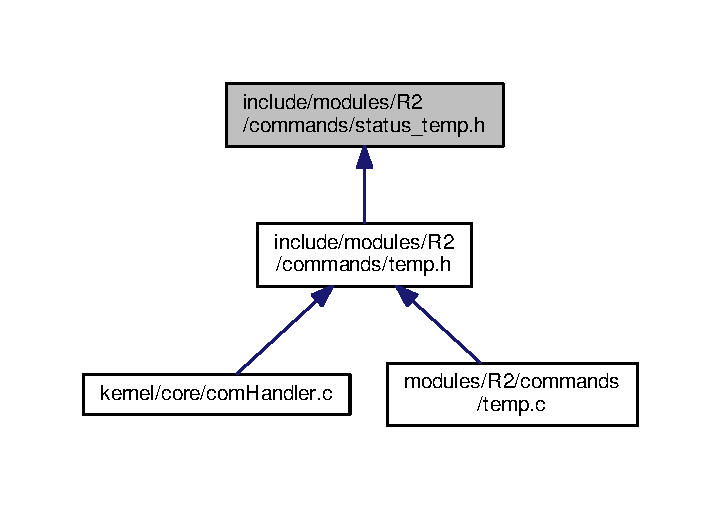
\includegraphics[width=346pt]{status__temp_8h__dep__incl}
\end{center}
\end{figure}
\subsection*{Macros}
\begin{DoxyCompactItemize}
\item 
\#define \hyperlink{status__temp_8h_ac77924329fd299922b865355c38a84cf}{C\+R\+E\+A\+T\+E\+\_\+\+P\+C\+B\+\_\+\+S\+U\+C\+C\+E\+SS}~((const char$\ast$) \char`\"{}P\+CB created successfully.\char`\"{})
\item 
\#define \hyperlink{status__temp_8h_ab96c6daf821f1eb62faee65336979a8f}{D\+E\+L\+E\+T\+E\+\_\+\+P\+C\+B\+\_\+\+S\+U\+C\+C\+E\+SS}~((const char$\ast$) \char`\"{}P\+CB deleted successfully.\char`\"{})
\item 
\#define \hyperlink{status__temp_8h_a6f9d8825dcf06847214ae1ff0d0fe33d}{B\+L\+O\+C\+K\+\_\+\+P\+C\+B\+\_\+\+S\+U\+C\+C\+E\+SS}~((const char$\ast$) \char`\"{}P\+CB set to blocked.\char`\"{})
\item 
\#define \hyperlink{status__temp_8h_a7dea081a0255c32868d0de0978f2d6cc}{U\+N\+B\+L\+O\+C\+K\+\_\+\+P\+C\+B\+\_\+\+S\+U\+C\+C\+E\+SS}~((const char$\ast$) \char`\"{}P\+CB set to unblocked.\char`\"{})
\item 
\#define \hyperlink{status__temp_8h_a18b4ed9cd81b7f35bf77d823cafd7320}{P\+R\+O\+C\+E\+S\+S\+\_\+\+N\+A\+M\+E\+\_\+\+A\+L\+R\+E\+A\+D\+Y\+\_\+\+E\+X\+I\+S\+TS}~((const char$\ast$) \char`\"{}This process name already exists\char`\"{})
\end{DoxyCompactItemize}


\subsection{Macro Definition Documentation}
\index{status\+\_\+temp.\+h@{status\+\_\+temp.\+h}!B\+L\+O\+C\+K\+\_\+\+P\+C\+B\+\_\+\+S\+U\+C\+C\+E\+SS@{B\+L\+O\+C\+K\+\_\+\+P\+C\+B\+\_\+\+S\+U\+C\+C\+E\+SS}}
\index{B\+L\+O\+C\+K\+\_\+\+P\+C\+B\+\_\+\+S\+U\+C\+C\+E\+SS@{B\+L\+O\+C\+K\+\_\+\+P\+C\+B\+\_\+\+S\+U\+C\+C\+E\+SS}!status\+\_\+temp.\+h@{status\+\_\+temp.\+h}}
\subsubsection[{\texorpdfstring{B\+L\+O\+C\+K\+\_\+\+P\+C\+B\+\_\+\+S\+U\+C\+C\+E\+SS}{BLOCK_PCB_SUCCESS}}]{\setlength{\rightskip}{0pt plus 5cm}\#define B\+L\+O\+C\+K\+\_\+\+P\+C\+B\+\_\+\+S\+U\+C\+C\+E\+SS~((const char$\ast$) \char`\"{}P\+CB set to blocked.\char`\"{})}\hypertarget{status__temp_8h_a6f9d8825dcf06847214ae1ff0d0fe33d}{}\label{status__temp_8h_a6f9d8825dcf06847214ae1ff0d0fe33d}
\index{status\+\_\+temp.\+h@{status\+\_\+temp.\+h}!C\+R\+E\+A\+T\+E\+\_\+\+P\+C\+B\+\_\+\+S\+U\+C\+C\+E\+SS@{C\+R\+E\+A\+T\+E\+\_\+\+P\+C\+B\+\_\+\+S\+U\+C\+C\+E\+SS}}
\index{C\+R\+E\+A\+T\+E\+\_\+\+P\+C\+B\+\_\+\+S\+U\+C\+C\+E\+SS@{C\+R\+E\+A\+T\+E\+\_\+\+P\+C\+B\+\_\+\+S\+U\+C\+C\+E\+SS}!status\+\_\+temp.\+h@{status\+\_\+temp.\+h}}
\subsubsection[{\texorpdfstring{C\+R\+E\+A\+T\+E\+\_\+\+P\+C\+B\+\_\+\+S\+U\+C\+C\+E\+SS}{CREATE_PCB_SUCCESS}}]{\setlength{\rightskip}{0pt plus 5cm}\#define C\+R\+E\+A\+T\+E\+\_\+\+P\+C\+B\+\_\+\+S\+U\+C\+C\+E\+SS~((const char$\ast$) \char`\"{}P\+CB created successfully.\char`\"{})}\hypertarget{status__temp_8h_ac77924329fd299922b865355c38a84cf}{}\label{status__temp_8h_ac77924329fd299922b865355c38a84cf}
\index{status\+\_\+temp.\+h@{status\+\_\+temp.\+h}!D\+E\+L\+E\+T\+E\+\_\+\+P\+C\+B\+\_\+\+S\+U\+C\+C\+E\+SS@{D\+E\+L\+E\+T\+E\+\_\+\+P\+C\+B\+\_\+\+S\+U\+C\+C\+E\+SS}}
\index{D\+E\+L\+E\+T\+E\+\_\+\+P\+C\+B\+\_\+\+S\+U\+C\+C\+E\+SS@{D\+E\+L\+E\+T\+E\+\_\+\+P\+C\+B\+\_\+\+S\+U\+C\+C\+E\+SS}!status\+\_\+temp.\+h@{status\+\_\+temp.\+h}}
\subsubsection[{\texorpdfstring{D\+E\+L\+E\+T\+E\+\_\+\+P\+C\+B\+\_\+\+S\+U\+C\+C\+E\+SS}{DELETE_PCB_SUCCESS}}]{\setlength{\rightskip}{0pt plus 5cm}\#define D\+E\+L\+E\+T\+E\+\_\+\+P\+C\+B\+\_\+\+S\+U\+C\+C\+E\+SS~((const char$\ast$) \char`\"{}P\+CB deleted successfully.\char`\"{})}\hypertarget{status__temp_8h_ab96c6daf821f1eb62faee65336979a8f}{}\label{status__temp_8h_ab96c6daf821f1eb62faee65336979a8f}
\index{status\+\_\+temp.\+h@{status\+\_\+temp.\+h}!P\+R\+O\+C\+E\+S\+S\+\_\+\+N\+A\+M\+E\+\_\+\+A\+L\+R\+E\+A\+D\+Y\+\_\+\+E\+X\+I\+S\+TS@{P\+R\+O\+C\+E\+S\+S\+\_\+\+N\+A\+M\+E\+\_\+\+A\+L\+R\+E\+A\+D\+Y\+\_\+\+E\+X\+I\+S\+TS}}
\index{P\+R\+O\+C\+E\+S\+S\+\_\+\+N\+A\+M\+E\+\_\+\+A\+L\+R\+E\+A\+D\+Y\+\_\+\+E\+X\+I\+S\+TS@{P\+R\+O\+C\+E\+S\+S\+\_\+\+N\+A\+M\+E\+\_\+\+A\+L\+R\+E\+A\+D\+Y\+\_\+\+E\+X\+I\+S\+TS}!status\+\_\+temp.\+h@{status\+\_\+temp.\+h}}
\subsubsection[{\texorpdfstring{P\+R\+O\+C\+E\+S\+S\+\_\+\+N\+A\+M\+E\+\_\+\+A\+L\+R\+E\+A\+D\+Y\+\_\+\+E\+X\+I\+S\+TS}{PROCESS_NAME_ALREADY_EXISTS}}]{\setlength{\rightskip}{0pt plus 5cm}\#define P\+R\+O\+C\+E\+S\+S\+\_\+\+N\+A\+M\+E\+\_\+\+A\+L\+R\+E\+A\+D\+Y\+\_\+\+E\+X\+I\+S\+TS~((const char$\ast$) \char`\"{}This process name already exists\char`\"{})}\hypertarget{status__temp_8h_a18b4ed9cd81b7f35bf77d823cafd7320}{}\label{status__temp_8h_a18b4ed9cd81b7f35bf77d823cafd7320}
\index{status\+\_\+temp.\+h@{status\+\_\+temp.\+h}!U\+N\+B\+L\+O\+C\+K\+\_\+\+P\+C\+B\+\_\+\+S\+U\+C\+C\+E\+SS@{U\+N\+B\+L\+O\+C\+K\+\_\+\+P\+C\+B\+\_\+\+S\+U\+C\+C\+E\+SS}}
\index{U\+N\+B\+L\+O\+C\+K\+\_\+\+P\+C\+B\+\_\+\+S\+U\+C\+C\+E\+SS@{U\+N\+B\+L\+O\+C\+K\+\_\+\+P\+C\+B\+\_\+\+S\+U\+C\+C\+E\+SS}!status\+\_\+temp.\+h@{status\+\_\+temp.\+h}}
\subsubsection[{\texorpdfstring{U\+N\+B\+L\+O\+C\+K\+\_\+\+P\+C\+B\+\_\+\+S\+U\+C\+C\+E\+SS}{UNBLOCK_PCB_SUCCESS}}]{\setlength{\rightskip}{0pt plus 5cm}\#define U\+N\+B\+L\+O\+C\+K\+\_\+\+P\+C\+B\+\_\+\+S\+U\+C\+C\+E\+SS~((const char$\ast$) \char`\"{}P\+CB set to unblocked.\char`\"{})}\hypertarget{status__temp_8h_a7dea081a0255c32868d0de0978f2d6cc}{}\label{status__temp_8h_a7dea081a0255c32868d0de0978f2d6cc}

\hypertarget{temp_8h}{}\section{include/modules/\+R2/commands/temp.h File Reference}
\label{temp_8h}\index{include/modules/\+R2/commands/temp.\+h@{include/modules/\+R2/commands/temp.\+h}}
{\ttfamily \#include \char`\"{}help\+\_\+temp.\+h\char`\"{}}\\*
{\ttfamily \#include \char`\"{}status.\+h\char`\"{}}\\*
{\ttfamily \#include \char`\"{}status\+\_\+temp.\+h\char`\"{}}\\*
Include dependency graph for temp.\+h\+:\nopagebreak
\begin{figure}[H]
\begin{center}
\leavevmode
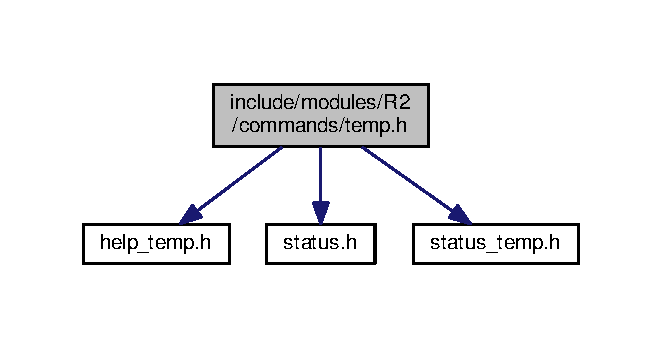
\includegraphics[width=318pt]{temp_8h__incl}
\end{center}
\end{figure}
This graph shows which files directly or indirectly include this file\+:\nopagebreak
\begin{figure}[H]
\begin{center}
\leavevmode
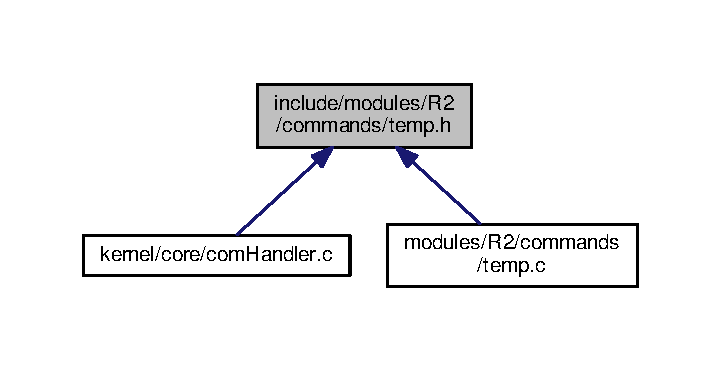
\includegraphics[width=346pt]{temp_8h__dep__incl}
\end{center}
\end{figure}
\subsection*{Functions}
\begin{DoxyCompactItemize}
\item 
void \hyperlink{temp_8h_a81189cb37f2afeab192231685edecd88}{register\+R2\+Temp\+Commands} ()
\item 
const char $\ast$ \hyperlink{temp_8h_a5e63afd4ae8abb41356eb748bef35d35}{create\+Pcb} (char $\ast$$\ast$args, int num\+Args)
\item 
const char $\ast$ \hyperlink{temp_8h_ab9749ddce5f9526746d36289fc41df80}{delete\+Pcb} (char $\ast$$\ast$args, int num\+Args)
\item 
const char $\ast$ \hyperlink{temp_8h_a679c0f302ee2c34f32fa616bc5e8353d}{block\+Pcb} (char $\ast$$\ast$args, int num\+Args)
\item 
const char $\ast$ \hyperlink{temp_8h_a9d9f1d27d45b617d33b361480b80e91f}{unblock\+Pcb} (char $\ast$$\ast$args, int num\+Args)
\end{DoxyCompactItemize}


\subsection{Function Documentation}
\index{temp.\+h@{temp.\+h}!block\+Pcb@{block\+Pcb}}
\index{block\+Pcb@{block\+Pcb}!temp.\+h@{temp.\+h}}
\subsubsection[{\texorpdfstring{block\+Pcb(char $\ast$$\ast$args, int num\+Args)}{blockPcb(char **args, int numArgs)}}]{\setlength{\rightskip}{0pt plus 5cm}const char$\ast$ block\+Pcb (
\begin{DoxyParamCaption}
\item[{char $\ast$$\ast$}]{args, }
\item[{int}]{num\+Args}
\end{DoxyParamCaption}
)}\hypertarget{temp_8h_a679c0f302ee2c34f32fa616bc5e8353d}{}\label{temp_8h_a679c0f302ee2c34f32fa616bc5e8353d}
Places a P\+CB into the blocked state and reinserts it into the appropriate queue.

Note\+: This command will be removed in module R3/\+R4

Usage\+: bpcb name

Args\+: name -\/ The Process Name to place into the blocked state (must exist)


\begin{DoxyParams}{Parameters}
{\em args} & The arguments to pass to the function \\
\hline
{\em num\+Args} & The number of arguments \\
\hline
\end{DoxyParams}
\begin{DoxyReturn}{Returns}
A status message indicating success/failure 
\end{DoxyReturn}
\index{temp.\+h@{temp.\+h}!create\+Pcb@{create\+Pcb}}
\index{create\+Pcb@{create\+Pcb}!temp.\+h@{temp.\+h}}
\subsubsection[{\texorpdfstring{create\+Pcb(char $\ast$$\ast$args, int num\+Args)}{createPcb(char **args, int numArgs)}}]{\setlength{\rightskip}{0pt plus 5cm}const char$\ast$ create\+Pcb (
\begin{DoxyParamCaption}
\item[{char $\ast$$\ast$}]{args, }
\item[{int}]{num\+Args}
\end{DoxyParamCaption}
)}\hypertarget{temp_8h_a5e63afd4ae8abb41356eb748bef35d35}{}\label{temp_8h_a5e63afd4ae8abb41356eb748bef35d35}
Creates a P\+CB and inserts it into the appropriate queue.

Note\+: This command will be removed in module R3/\+R4

Usage\+: cpcb name class priority

Args\+: name -\/ The Process Name (must be unique) class -\/ The Process Class (either 0 (system) or 1 (application)) priority -\/ The Process Priority (number between 0 and 9)


\begin{DoxyParams}{Parameters}
{\em args} & The arguments to pass to the function \\
\hline
{\em num\+Args} & The number of arguments \\
\hline
\end{DoxyParams}
\begin{DoxyReturn}{Returns}
A status message indicating success/failure 
\end{DoxyReturn}
\index{temp.\+h@{temp.\+h}!delete\+Pcb@{delete\+Pcb}}
\index{delete\+Pcb@{delete\+Pcb}!temp.\+h@{temp.\+h}}
\subsubsection[{\texorpdfstring{delete\+Pcb(char $\ast$$\ast$args, int num\+Args)}{deletePcb(char **args, int numArgs)}}]{\setlength{\rightskip}{0pt plus 5cm}const char$\ast$ delete\+Pcb (
\begin{DoxyParamCaption}
\item[{char $\ast$$\ast$}]{args, }
\item[{int}]{num\+Args}
\end{DoxyParamCaption}
)}\hypertarget{temp_8h_ab9749ddce5f9526746d36289fc41df80}{}\label{temp_8h_ab9749ddce5f9526746d36289fc41df80}
Removes a P\+CB from the appropriate queue and then frees all associated memory.

Note\+: This command will be removed in module R3/\+R4

Usage\+: dpcb name

Args\+: name -\/ The Process Name to remove (must exist)


\begin{DoxyParams}{Parameters}
{\em args} & The arguments to pass to the function \\
\hline
{\em num\+Args} & The number of arguments \\
\hline
\end{DoxyParams}
\begin{DoxyReturn}{Returns}
A status message indicating success/failure 
\end{DoxyReturn}
\index{temp.\+h@{temp.\+h}!register\+R2\+Temp\+Commands@{register\+R2\+Temp\+Commands}}
\index{register\+R2\+Temp\+Commands@{register\+R2\+Temp\+Commands}!temp.\+h@{temp.\+h}}
\subsubsection[{\texorpdfstring{register\+R2\+Temp\+Commands()}{registerR2TempCommands()}}]{\setlength{\rightskip}{0pt plus 5cm}void register\+R2\+Temp\+Commands (
\begin{DoxyParamCaption}
{}
\end{DoxyParamCaption}
)}\hypertarget{temp_8h_a81189cb37f2afeab192231685edecd88}{}\label{temp_8h_a81189cb37f2afeab192231685edecd88}
Registers the temporary commands in the command handler \index{temp.\+h@{temp.\+h}!unblock\+Pcb@{unblock\+Pcb}}
\index{unblock\+Pcb@{unblock\+Pcb}!temp.\+h@{temp.\+h}}
\subsubsection[{\texorpdfstring{unblock\+Pcb(char $\ast$$\ast$args, int num\+Args)}{unblockPcb(char **args, int numArgs)}}]{\setlength{\rightskip}{0pt plus 5cm}const char$\ast$ unblock\+Pcb (
\begin{DoxyParamCaption}
\item[{char $\ast$$\ast$}]{args, }
\item[{int}]{num\+Args}
\end{DoxyParamCaption}
)}\hypertarget{temp_8h_a9d9f1d27d45b617d33b361480b80e91f}{}\label{temp_8h_a9d9f1d27d45b617d33b361480b80e91f}
Places a P\+CB into the unblocked state and reinserts it into the appropriate queue.

Note\+: This command will be removed in module R3/\+R4

Usage\+: upcb name

Args\+: name -\/ The Process Name to place into the unblocked state (must exist)


\begin{DoxyParams}{Parameters}
{\em args} & The arguments to pass to the function \\
\hline
{\em num\+Args} & The number of arguments \\
\hline
\end{DoxyParams}
\begin{DoxyReturn}{Returns}
A status message indicating success/failure 
\end{DoxyReturn}

\hypertarget{r3commands_8h}{}\section{include/modules/\+R3/commands/r3commands.h File Reference}
\label{r3commands_8h}\index{include/modules/\+R3/commands/r3commands.\+h@{include/modules/\+R3/commands/r3commands.\+h}}
{\ttfamily \#include $<$modules/\+R3/commands/help.\+h$>$}\\*
Include dependency graph for r3commands.\+h\+:\nopagebreak
\begin{figure}[H]
\begin{center}
\leavevmode
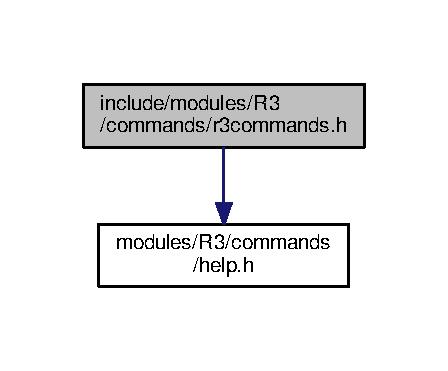
\includegraphics[width=215pt]{r3commands_8h__incl}
\end{center}
\end{figure}
This graph shows which files directly or indirectly include this file\+:\nopagebreak
\begin{figure}[H]
\begin{center}
\leavevmode
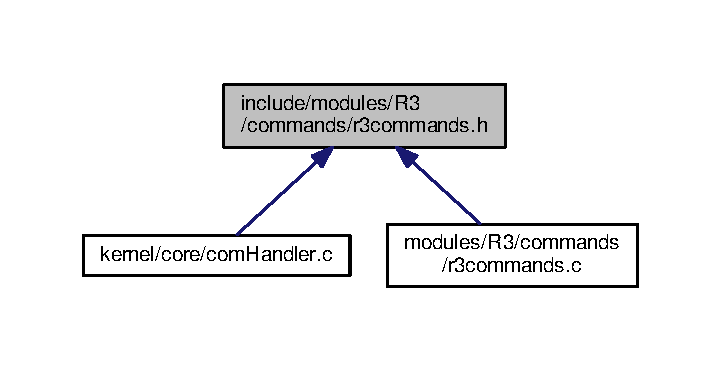
\includegraphics[width=346pt]{r3commands_8h__dep__incl}
\end{center}
\end{figure}
\subsection*{Functions}
\begin{DoxyCompactItemize}
\item 
void \hyperlink{r3commands_8h_ac3eaf8777396a53fec4521ca264f5dcc}{register\+R3\+Commands} ()
\item 
const char $\ast$ \hyperlink{r3commands_8h_a560ff05de4721b7ee4008437c4597cd3}{yield} (char $\ast$$\ast$args, int num\+Args)
\item 
const char $\ast$ \hyperlink{r3commands_8h_ac06ea22234ec47eb995772ac6d355743}{loadr3} (char $\ast$$\ast$args, int num\+Args)
\end{DoxyCompactItemize}


\subsection{Function Documentation}
\index{r3commands.\+h@{r3commands.\+h}!loadr3@{loadr3}}
\index{loadr3@{loadr3}!r3commands.\+h@{r3commands.\+h}}
\subsubsection[{\texorpdfstring{loadr3(char $\ast$$\ast$args, int num\+Args)}{loadr3(char **args, int numArgs)}}]{\setlength{\rightskip}{0pt plus 5cm}const char$\ast$ loadr3 (
\begin{DoxyParamCaption}
\item[{char $\ast$$\ast$}]{args, }
\item[{int}]{num\+Args}
\end{DoxyParamCaption}
)}\hypertarget{r3commands_8h_ac06ea22234ec47eb995772ac6d355743}{}\label{r3commands_8h_ac06ea22234ec47eb995772ac6d355743}
Loads the r3 processes to the queue.~\newline
")

Usage\+: loadr3

Args\+: \mbox{[}no args\mbox{]} -\/ loads processes


\begin{DoxyParams}{Parameters}
{\em args} & The arguments to pass to the function \\
\hline
\end{DoxyParams}
\begin{DoxyReturn}{Returns}
\char`\"{}\char`\"{} 
\end{DoxyReturn}
\index{r3commands.\+h@{r3commands.\+h}!register\+R3\+Commands@{register\+R3\+Commands}}
\index{register\+R3\+Commands@{register\+R3\+Commands}!r3commands.\+h@{r3commands.\+h}}
\subsubsection[{\texorpdfstring{register\+R3\+Commands()}{registerR3Commands()}}]{\setlength{\rightskip}{0pt plus 5cm}void register\+R3\+Commands (
\begin{DoxyParamCaption}
{}
\end{DoxyParamCaption}
)}\hypertarget{r3commands_8h_ac3eaf8777396a53fec4521ca264f5dcc}{}\label{r3commands_8h_ac3eaf8777396a53fec4521ca264f5dcc}
Registers commands in command handler \index{r3commands.\+h@{r3commands.\+h}!yield@{yield}}
\index{yield@{yield}!r3commands.\+h@{r3commands.\+h}}
\subsubsection[{\texorpdfstring{yield(char $\ast$$\ast$args, int num\+Args)}{yield(char **args, int numArgs)}}]{\setlength{\rightskip}{0pt plus 5cm}const char$\ast$ yield (
\begin{DoxyParamCaption}
\item[{char $\ast$$\ast$}]{args, }
\item[{int}]{num\+Args}
\end{DoxyParamCaption}
)}\hypertarget{r3commands_8h_a560ff05de4721b7ee4008437c4597cd3}{}\label{r3commands_8h_a560ff05de4721b7ee4008437c4597cd3}
Yields command handler to allow other processes to run.

Usage\+: yield

Args\+: \mbox{[}no args\mbox{]} -\/ yields command handler


\begin{DoxyParams}{Parameters}
{\em args} & The arguments to pass to the function \\
\hline
\end{DoxyParams}
\begin{DoxyReturn}{Returns}
\char`\"{}\char`\"{} 
\end{DoxyReturn}

\hypertarget{processes_8h}{}\section{include/modules/\+R3/processes.h File Reference}
\label{processes_8h}\index{include/modules/\+R3/processes.\+h@{include/modules/\+R3/processes.\+h}}
This graph shows which files directly or indirectly include this file\+:\nopagebreak
\begin{figure}[H]
\begin{center}
\leavevmode
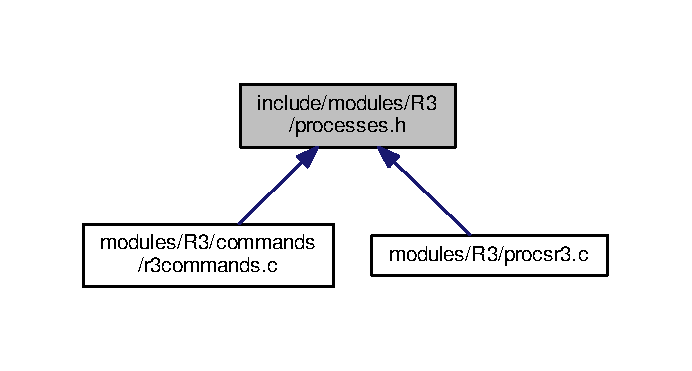
\includegraphics[width=332pt]{processes_8h__dep__incl}
\end{center}
\end{figure}
\subsection*{Functions}
\begin{DoxyCompactItemize}
\item 
void \hyperlink{processes_8h_ade99845b64379d4ca17724eb6e39c2b4}{proc1} ()
\item 
void \hyperlink{processes_8h_af37cd4c55ba62a3241f54f8f4e8747e8}{proc2} ()
\item 
void \hyperlink{processes_8h_aea8e61640dff07a97542c429e0eb2559}{proc3} ()
\item 
void \hyperlink{processes_8h_a86a94995afad1e25eaab374c95c89c94}{proc4} ()
\item 
void \hyperlink{processes_8h_a6c2f639619099a32f0b4004bd111d679}{proc5} ()
\end{DoxyCompactItemize}


\subsection{Function Documentation}
\index{processes.\+h@{processes.\+h}!proc1@{proc1}}
\index{proc1@{proc1}!processes.\+h@{processes.\+h}}
\subsubsection[{\texorpdfstring{proc1()}{proc1()}}]{\setlength{\rightskip}{0pt plus 5cm}void proc1 (
\begin{DoxyParamCaption}
{}
\end{DoxyParamCaption}
)}\hypertarget{processes_8h_ade99845b64379d4ca17724eb6e39c2b4}{}\label{processes_8h_ade99845b64379d4ca17724eb6e39c2b4}
\index{processes.\+h@{processes.\+h}!proc2@{proc2}}
\index{proc2@{proc2}!processes.\+h@{processes.\+h}}
\subsubsection[{\texorpdfstring{proc2()}{proc2()}}]{\setlength{\rightskip}{0pt plus 5cm}void proc2 (
\begin{DoxyParamCaption}
{}
\end{DoxyParamCaption}
)}\hypertarget{processes_8h_af37cd4c55ba62a3241f54f8f4e8747e8}{}\label{processes_8h_af37cd4c55ba62a3241f54f8f4e8747e8}
\index{processes.\+h@{processes.\+h}!proc3@{proc3}}
\index{proc3@{proc3}!processes.\+h@{processes.\+h}}
\subsubsection[{\texorpdfstring{proc3()}{proc3()}}]{\setlength{\rightskip}{0pt plus 5cm}void proc3 (
\begin{DoxyParamCaption}
{}
\end{DoxyParamCaption}
)}\hypertarget{processes_8h_aea8e61640dff07a97542c429e0eb2559}{}\label{processes_8h_aea8e61640dff07a97542c429e0eb2559}
\index{processes.\+h@{processes.\+h}!proc4@{proc4}}
\index{proc4@{proc4}!processes.\+h@{processes.\+h}}
\subsubsection[{\texorpdfstring{proc4()}{proc4()}}]{\setlength{\rightskip}{0pt plus 5cm}void proc4 (
\begin{DoxyParamCaption}
{}
\end{DoxyParamCaption}
)}\hypertarget{processes_8h_a86a94995afad1e25eaab374c95c89c94}{}\label{processes_8h_a86a94995afad1e25eaab374c95c89c94}
\index{processes.\+h@{processes.\+h}!proc5@{proc5}}
\index{proc5@{proc5}!processes.\+h@{processes.\+h}}
\subsubsection[{\texorpdfstring{proc5()}{proc5()}}]{\setlength{\rightskip}{0pt plus 5cm}void proc5 (
\begin{DoxyParamCaption}
{}
\end{DoxyParamCaption}
)}\hypertarget{processes_8h_a6c2f639619099a32f0b4004bd111d679}{}\label{processes_8h_a6c2f639619099a32f0b4004bd111d679}

\hypertarget{r5commands_8h}{}\section{include/modules/\+R5/commands/r5commands.h File Reference}
\label{r5commands_8h}\index{include/modules/\+R5/commands/r5commands.\+h@{include/modules/\+R5/commands/r5commands.\+h}}
{\ttfamily \#include $<$modules/\+R5/commands/help.\+h$>$}\\*
Include dependency graph for r5commands.\+h\+:\nopagebreak
\begin{figure}[H]
\begin{center}
\leavevmode
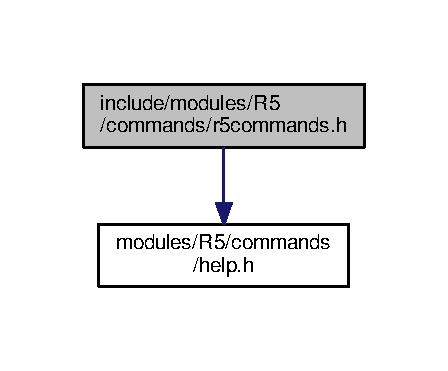
\includegraphics[width=215pt]{r5commands_8h__incl}
\end{center}
\end{figure}
This graph shows which files directly or indirectly include this file\+:\nopagebreak
\begin{figure}[H]
\begin{center}
\leavevmode
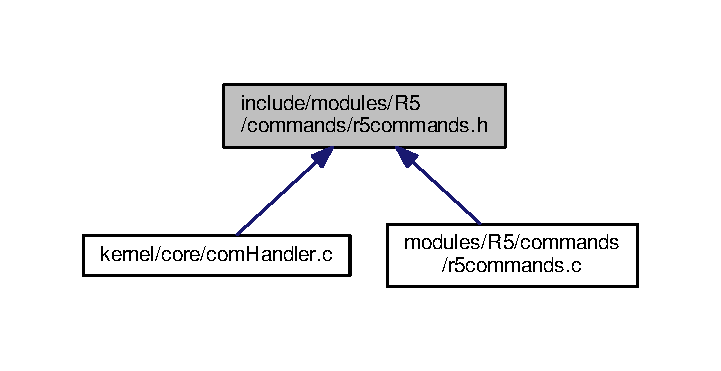
\includegraphics[width=346pt]{r5commands_8h__dep__incl}
\end{center}
\end{figure}
\subsection*{Functions}
\begin{DoxyCompactItemize}
\item 
void \hyperlink{r5commands_8h_a21eac9fef5e4c61e3c5e516237dfd611}{register\+R5\+Perm\+Commands} ()
\item 
const char $\ast$ \hyperlink{r5commands_8h_a2213472154067610a41f70642395892b}{show\+Memory} (char $\ast$$\ast$args, int num\+Args)
\end{DoxyCompactItemize}


\subsection{Function Documentation}
\index{r5commands.\+h@{r5commands.\+h}!register\+R5\+Perm\+Commands@{register\+R5\+Perm\+Commands}}
\index{register\+R5\+Perm\+Commands@{register\+R5\+Perm\+Commands}!r5commands.\+h@{r5commands.\+h}}
\subsubsection[{\texorpdfstring{register\+R5\+Perm\+Commands()}{registerR5PermCommands()}}]{\setlength{\rightskip}{0pt plus 5cm}void register\+R5\+Perm\+Commands (
\begin{DoxyParamCaption}
{}
\end{DoxyParamCaption}
)}\hypertarget{r5commands_8h_a21eac9fef5e4c61e3c5e516237dfd611}{}\label{r5commands_8h_a21eac9fef5e4c61e3c5e516237dfd611}
Registers commands in command handler

Registers the permanent commands in the command handler \index{r5commands.\+h@{r5commands.\+h}!show\+Memory@{show\+Memory}}
\index{show\+Memory@{show\+Memory}!r5commands.\+h@{r5commands.\+h}}
\subsubsection[{\texorpdfstring{show\+Memory(char $\ast$$\ast$args, int num\+Args)}{showMemory(char **args, int numArgs)}}]{\setlength{\rightskip}{0pt plus 5cm}const char$\ast$ show\+Memory (
\begin{DoxyParamCaption}
\item[{char $\ast$$\ast$}]{args, }
\item[{int}]{num\+Args}
\end{DoxyParamCaption}
)}\hypertarget{r5commands_8h_a2213472154067610a41f70642395892b}{}\label{r5commands_8h_a2213472154067610a41f70642395892b}
Displays the following information for the specified C\+M\+CB\textquotesingle{}s\+: C\+M\+CB Type\+: Begining Memory Address\+: Block Size\+: Memory Size\+: Process Name\+:

Usage\+: show\+Memory \mbox{[}--all\mbox{]} \mbox{[}--free\mbox{]} \mbox{[}--allocated\mbox{]}

Args\+: \mbox{[}no args\mbox{]} -\/ Shows the help for this command --all -\/ Displays both free and allocated memory --free -\/ Displays free memory --allocated -\/ Displays allocated memory


\begin{DoxyParams}{Parameters}
{\em args} & The arguments to pass to the function \\
\hline
{\em num\+Args} & The number of arguments \\
\hline
\end{DoxyParams}
\begin{DoxyReturn}{Returns}
A status message indicating success/failure 
\end{DoxyReturn}

\hypertarget{mem_commands_8h}{}\section{include/modules/\+R5/mem\+Commands.h File Reference}
\label{mem_commands_8h}\index{include/modules/\+R5/mem\+Commands.\+h@{include/modules/\+R5/mem\+Commands.\+h}}
{\ttfamily \#include $<$mem/memory\+Control.\+h$>$}\\*
{\ttfamily \#include $<$boolean.\+h$>$}\\*
{\ttfamily \#include $<$core/com\+Handler.\+h$>$}\\*
{\ttfamily \#include $<$core/help.\+h$>$}\\*
{\ttfamily \#include $<$modules/\+R5/help.\+h$>$}\\*
{\ttfamily \#include $<$modules/mpx\+\_\+supt.\+h$>$}\\*
Include dependency graph for mem\+Commands.\+h\+:\nopagebreak
\begin{figure}[H]
\begin{center}
\leavevmode
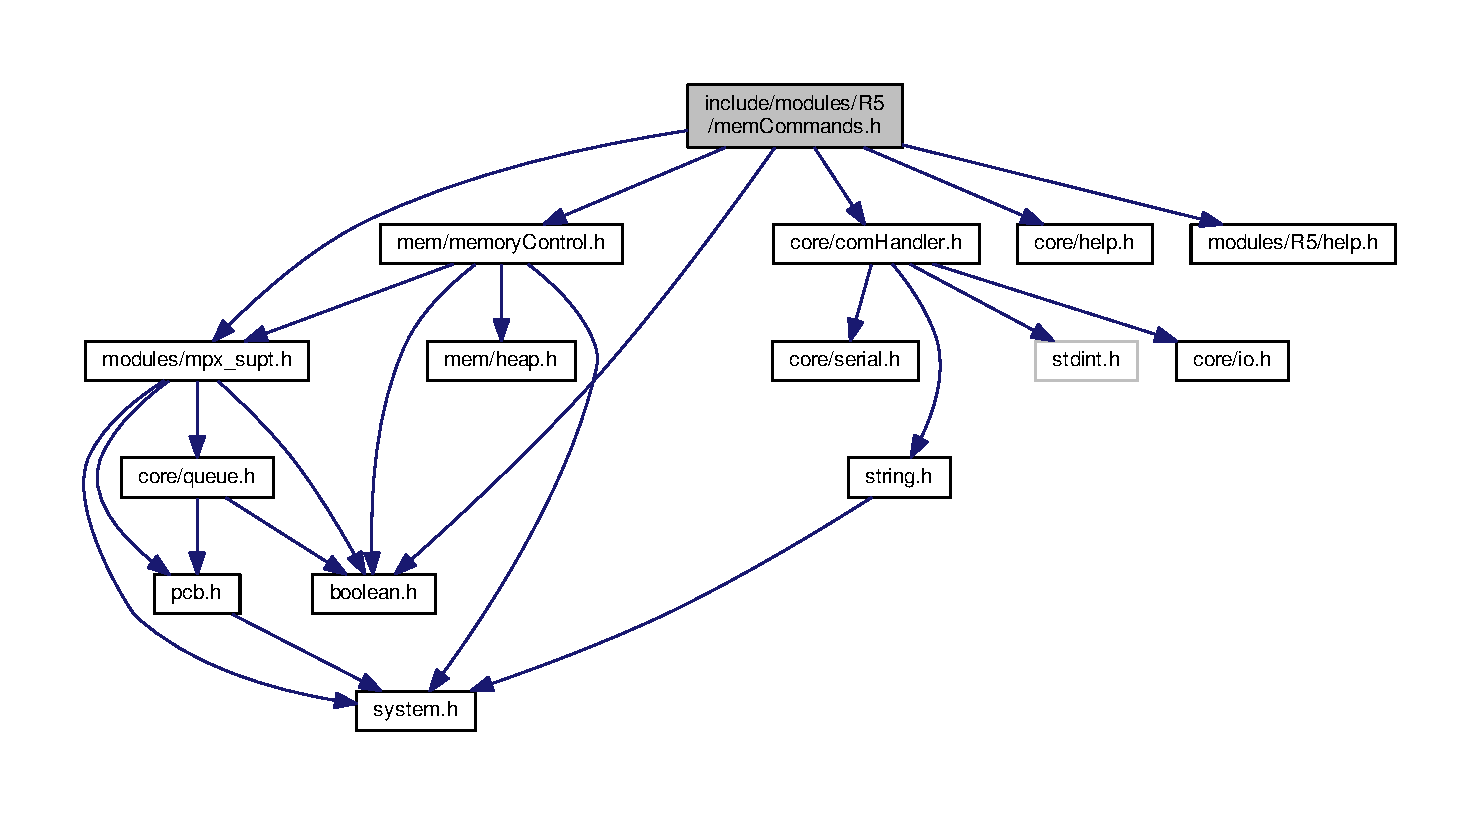
\includegraphics[width=350pt]{mem_commands_8h__incl}
\end{center}
\end{figure}
This graph shows which files directly or indirectly include this file\+:\nopagebreak
\begin{figure}[H]
\begin{center}
\leavevmode
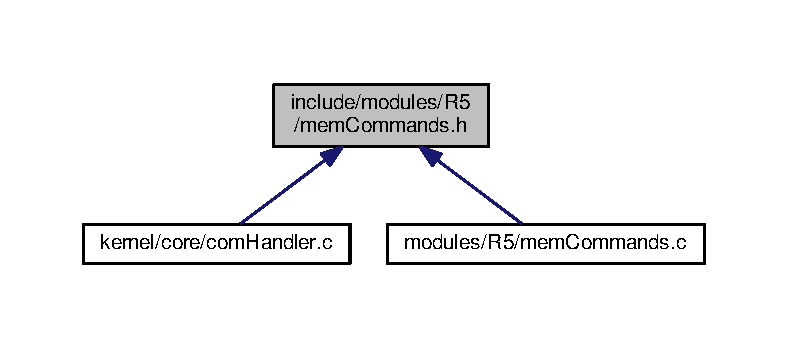
\includegraphics[width=350pt]{mem_commands_8h__dep__incl}
\end{center}
\end{figure}
\subsection*{Functions}
\begin{DoxyCompactItemize}
\item 
void \hyperlink{mem_commands_8h_a7ac22a33e0c40829431c45c393ef3ece}{register\+R5\+Temp\+Commands} ()
\item 
const char $\ast$ \hyperlink{mem_commands_8h_a26a3d6f0c06211cf1fdb0d69febb0624}{init\+Heap} (char $\ast$$\ast$args, int num\+Args)
\item 
const char $\ast$ \hyperlink{mem_commands_8h_a8c34ba132332867bae929ac6bce37cc7}{allocate\+Mem} (char $\ast$$\ast$args, int num\+Args)
\item 
const char $\ast$ \hyperlink{mem_commands_8h_a5cb6fcfaf13055b8a30f1b4def59699c}{free\+Memory} (char $\ast$$\ast$args, int num\+Args)
\item 
const char $\ast$ \hyperlink{mem_commands_8h_afa60e4452b25cba25054ba9319184a8c}{is\+Empty\+Com} (char $\ast$$\ast$args, int num\+Args)
\end{DoxyCompactItemize}


\subsection{Function Documentation}
\index{mem\+Commands.\+h@{mem\+Commands.\+h}!allocate\+Mem@{allocate\+Mem}}
\index{allocate\+Mem@{allocate\+Mem}!mem\+Commands.\+h@{mem\+Commands.\+h}}
\subsubsection[{\texorpdfstring{allocate\+Mem(char $\ast$$\ast$args, int num\+Args)}{allocateMem(char **args, int numArgs)}}]{\setlength{\rightskip}{0pt plus 5cm}const char$\ast$ allocate\+Mem (
\begin{DoxyParamCaption}
\item[{char $\ast$$\ast$}]{args, }
\item[{int}]{num\+Args}
\end{DoxyParamCaption}
)}\hypertarget{mem_commands_8h_a8c34ba132332867bae929ac6bce37cc7}{}\label{mem_commands_8h_a8c34ba132332867bae929ac6bce37cc7}
Allocates a memory block if enough memory is availabel


\begin{DoxyParams}{Parameters}
{\em size} & -\/ size of memory to allocate in bytes \\
\hline
\end{DoxyParams}
\begin{DoxyReturn}{Returns}
pointer to the me
\end{DoxyReturn}
Allocates a memory block if enough memory is available


\begin{DoxyParams}{Parameters}
{\em size} & -\/ size of memory to allocate in bytes \\
\hline
\end{DoxyParams}
\begin{DoxyReturn}{Returns}
pointer to the me 
\end{DoxyReturn}
\index{mem\+Commands.\+h@{mem\+Commands.\+h}!free\+Memory@{free\+Memory}}
\index{free\+Memory@{free\+Memory}!mem\+Commands.\+h@{mem\+Commands.\+h}}
\subsubsection[{\texorpdfstring{free\+Memory(char $\ast$$\ast$args, int num\+Args)}{freeMemory(char **args, int numArgs)}}]{\setlength{\rightskip}{0pt plus 5cm}const char$\ast$ free\+Memory (
\begin{DoxyParamCaption}
\item[{char $\ast$$\ast$}]{args, }
\item[{int}]{num\+Args}
\end{DoxyParamCaption}
)}\hypertarget{mem_commands_8h_a5cb6fcfaf13055b8a30f1b4def59699c}{}\label{mem_commands_8h_a5cb6fcfaf13055b8a30f1b4def59699c}
Deallocates the block of memory at the mempointer


\begin{DoxyParams}{Parameters}
{\em mem\+Pointer} & -\/ pointer to the mem block \\
\hline
\end{DoxyParams}
\index{mem\+Commands.\+h@{mem\+Commands.\+h}!init\+Heap@{init\+Heap}}
\index{init\+Heap@{init\+Heap}!mem\+Commands.\+h@{mem\+Commands.\+h}}
\subsubsection[{\texorpdfstring{init\+Heap(char $\ast$$\ast$args, int num\+Args)}{initHeap(char **args, int numArgs)}}]{\setlength{\rightskip}{0pt plus 5cm}const char$\ast$ init\+Heap (
\begin{DoxyParamCaption}
\item[{char $\ast$$\ast$}]{args, }
\item[{int}]{num\+Args}
\end{DoxyParamCaption}
)}\hypertarget{mem_commands_8h_a26a3d6f0c06211cf1fdb0d69febb0624}{}\label{mem_commands_8h_a26a3d6f0c06211cf1fdb0d69febb0624}
Initializes the heap to the provided size and creates a free mem block across it

\begin{DoxyReturn}{Returns}
True or false 
\end{DoxyReturn}
\index{mem\+Commands.\+h@{mem\+Commands.\+h}!is\+Empty\+Com@{is\+Empty\+Com}}
\index{is\+Empty\+Com@{is\+Empty\+Com}!mem\+Commands.\+h@{mem\+Commands.\+h}}
\subsubsection[{\texorpdfstring{is\+Empty\+Com(char $\ast$$\ast$args, int num\+Args)}{isEmptyCom(char **args, int numArgs)}}]{\setlength{\rightskip}{0pt plus 5cm}const char$\ast$ is\+Empty\+Com (
\begin{DoxyParamCaption}
\item[{char $\ast$$\ast$}]{args, }
\item[{int}]{num\+Args}
\end{DoxyParamCaption}
)}\hypertarget{mem_commands_8h_afa60e4452b25cba25054ba9319184a8c}{}\label{mem_commands_8h_afa60e4452b25cba25054ba9319184a8c}
Check if memory is empty \index{mem\+Commands.\+h@{mem\+Commands.\+h}!register\+R5\+Temp\+Commands@{register\+R5\+Temp\+Commands}}
\index{register\+R5\+Temp\+Commands@{register\+R5\+Temp\+Commands}!mem\+Commands.\+h@{mem\+Commands.\+h}}
\subsubsection[{\texorpdfstring{register\+R5\+Temp\+Commands()}{registerR5TempCommands()}}]{\setlength{\rightskip}{0pt plus 5cm}void register\+R5\+Temp\+Commands (
\begin{DoxyParamCaption}
{}
\end{DoxyParamCaption}
)}\hypertarget{mem_commands_8h_a7ac22a33e0c40829431c45c393ef3ece}{}\label{mem_commands_8h_a7ac22a33e0c40829431c45c393ef3ece}
Registers the permanent commands in the command handler 
\hypertarget{regex_8h}{}\section{include/regex.h File Reference}
\label{regex_8h}\index{include/regex.\+h@{include/regex.\+h}}
This graph shows which files directly or indirectly include this file\+:\nopagebreak
\begin{figure}[H]
\begin{center}
\leavevmode
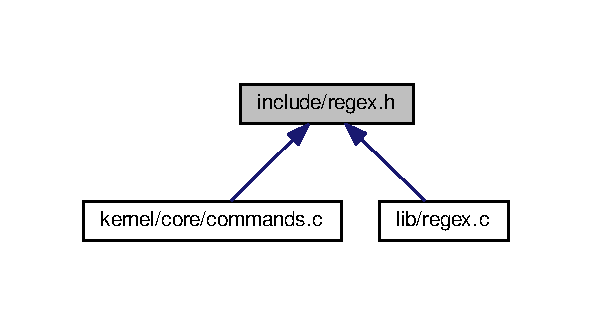
\includegraphics[width=284pt]{regex_8h__dep__incl}
\end{center}
\end{figure}
\subsection*{Functions}
\begin{DoxyCompactItemize}
\item 
int \hyperlink{regex_8h_a7ee5ec72fdd808d5959aa552df970761}{test\+Regex} (const char $\ast$regex, const char $\ast$string\+To\+Check)
\end{DoxyCompactItemize}


\subsection{Function Documentation}
\index{regex.\+h@{regex.\+h}!test\+Regex@{test\+Regex}}
\index{test\+Regex@{test\+Regex}!regex.\+h@{regex.\+h}}
\subsubsection[{\texorpdfstring{test\+Regex(const char $\ast$regex, const char $\ast$string\+To\+Check)}{testRegex(const char *regex, const char *stringToCheck)}}]{\setlength{\rightskip}{0pt plus 5cm}int test\+Regex (
\begin{DoxyParamCaption}
\item[{const char $\ast$}]{regex, }
\item[{const char $\ast$}]{string\+To\+Check}
\end{DoxyParamCaption}
)}\hypertarget{regex_8h_a7ee5ec72fdd808d5959aa552df970761}{}\label{regex_8h_a7ee5ec72fdd808d5959aa552df970761}
Tests if the string\+To\+Check adheres to the given regex string

The regex string is comprised of\+: d matches digits 0-\/9 c matches characters a-\/z\+A-\/Z u matches uppercase character, A-\/Z l matches lowercase character, a-\/z
\begin{DoxyItemize}
\item matches any char /char for a literal character, ex\+: \char`\"{}/a\char`\"{} matches \textquotesingle{}a\textquotesingle{}, /d matches \textquotesingle{}d\textquotesingle{}
\end{DoxyItemize}

Example \+: regex \char`\"{}dcd/a\char`\"{} matches any string with the pattern \char`\"{}digit character digit \textquotesingle{}a\textquotesingle{}\char`\"{}, ex \char`\"{}1b3a\char`\"{}, \char`\"{}6b9a\char`\"{}


\begin{DoxyParams}{Parameters}
{\em regex} & \\
\hline
{\em string\+To\+Check} & \\
\hline
\end{DoxyParams}
\begin{DoxyReturn}{Returns}
1 if adheres, 0 otherwise 
\end{DoxyReturn}

\hypertarget{string_8h}{}\section{include/string.h File Reference}
\label{string_8h}\index{include/string.\+h@{include/string.\+h}}
{\ttfamily \#include $<$system.\+h$>$}\\*
Include dependency graph for string.\+h\+:\nopagebreak
\begin{figure}[H]
\begin{center}
\leavevmode
\includegraphics[width=163pt]{string_8h__incl}
\end{center}
\end{figure}
This graph shows which files directly or indirectly include this file\+:
\nopagebreak
\begin{figure}[H]
\begin{center}
\leavevmode
\includegraphics[width=350pt]{string_8h__dep__incl}
\end{center}
\end{figure}
\subsection*{Functions}
\begin{DoxyCompactItemize}
\item 
int \hyperlink{string_8h_a0f3d37d605e9e6d4fc1853ff9d4b91bf}{isspace} (const char $\ast$c)
\item 
int \hyperlink{string_8h_a6a2b9960cc4b26c5e76ef56a1c233a95}{isdigit} (const char c)
\item 
int \hyperlink{string_8h_a1fabc9e88c2332828090cb7d716c7db9}{is\+Char} (const char c)
\item 
int \hyperlink{string_8h_ab1fd9310dd20b229c2701f3fb7608830}{is\+Upper\+Char} (const char c)
\item 
int \hyperlink{string_8h_a37c3a81183e47d54cdbfa1cf74cb45f7}{is\+Lower\+Char} (const char c)
\item 
char $\ast$ \hyperlink{string_8h_a1eb9cae61e6a6282c28dbc298ef7297e}{strcpy} (char $\ast$s1, const char $\ast$s2)
\item 
char $\ast$ \hyperlink{string_8h_a8908188ae9fc2f05d993257ef001d553}{strcat} (char $\ast$s1, const char $\ast$s2)
\item 
int \hyperlink{string_8h_a2dee044e4e667b5b789b493abd21cfa4}{strlen} (const char $\ast$s)
\item 
int \hyperlink{string_8h_a11bd144d7d44914099a3aeddf1c8567d}{strcmp} (const char $\ast$s1, const char $\ast$s2)
\item 
char $\ast$ \hyperlink{string_8h_af1a867dcea42fc1215d0eddf19283ef3}{strtok} (char $\ast$s1, const char $\ast$s2)
\item 
int \hyperlink{string_8h_a30670a60464f77af17dfb353353d6df8}{atoi} (const char $\ast$s)
\item 
void \hyperlink{string_8h_ad54d5e6d2a62cac148aa89737ed96236}{itoa} (int num, char $\ast$str, int \hyperlink{tables_8h_ab5763c2b18c825c8b8fba44b2e60ddc1}{base})
\item 
void \hyperlink{string_8h_aad7fea725cb4b198ace1aa3df5051244}{reverse} (char $\ast$str, int len)
\end{DoxyCompactItemize}


\subsection{Function Documentation}
\index{string.\+h@{string.\+h}!atoi@{atoi}}
\index{atoi@{atoi}!string.\+h@{string.\+h}}
\subsubsection[{\texorpdfstring{atoi(const char $\ast$s)}{atoi(const char *s)}}]{\setlength{\rightskip}{0pt plus 5cm}int atoi (
\begin{DoxyParamCaption}
\item[{const char $\ast$}]{s}
\end{DoxyParamCaption}
)}\hypertarget{string_8h_a30670a60464f77af17dfb353353d6df8}{}\label{string_8h_a30670a60464f77af17dfb353353d6df8}
Convert an A\+S\+C\+II string to an integer


\begin{DoxyParams}{Parameters}
{\em s} & The string to convert \\
\hline
\end{DoxyParams}
\begin{DoxyReturn}{Returns}
The integer value of the string, or the M\+A\+X/\+M\+IN value of an integer if the value is out of range. 
\end{DoxyReturn}
\index{string.\+h@{string.\+h}!is\+Char@{is\+Char}}
\index{is\+Char@{is\+Char}!string.\+h@{string.\+h}}
\subsubsection[{\texorpdfstring{is\+Char(const char c)}{isChar(const char c)}}]{\setlength{\rightskip}{0pt plus 5cm}int is\+Char (
\begin{DoxyParamCaption}
\item[{const char}]{c}
\end{DoxyParamCaption}
)}\hypertarget{string_8h_a1fabc9e88c2332828090cb7d716c7db9}{}\label{string_8h_a1fabc9e88c2332828090cb7d716c7db9}
Checks if the given char is a-\/z or A-\/Z 
\begin{DoxyParams}{Parameters}
{\em const} & char c \\
\hline
\end{DoxyParams}
\begin{DoxyReturn}{Returns}
1 if c is a char, 0 otherwies
\end{DoxyReturn}
Checks if the given char is a-\/z or A-\/Z 
\begin{DoxyParams}{Parameters}
{\em const} & char c \\
\hline
\end{DoxyParams}
\begin{DoxyReturn}{Returns}
1 if c is a char, 0 otherwise 
\end{DoxyReturn}
\index{string.\+h@{string.\+h}!isdigit@{isdigit}}
\index{isdigit@{isdigit}!string.\+h@{string.\+h}}
\subsubsection[{\texorpdfstring{isdigit(const char c)}{isdigit(const char c)}}]{\setlength{\rightskip}{0pt plus 5cm}int isdigit (
\begin{DoxyParamCaption}
\item[{const char}]{c}
\end{DoxyParamCaption}
)}\hypertarget{string_8h_a6a2b9960cc4b26c5e76ef56a1c233a95}{}\label{string_8h_a6a2b9960cc4b26c5e76ef56a1c233a95}
Determine if a character is a digit.


\begin{DoxyParams}{Parameters}
{\em c} & The character to check \\
\hline
\end{DoxyParams}
\begin{DoxyReturn}{Returns}
True if the character is a digit 
\end{DoxyReturn}
\index{string.\+h@{string.\+h}!is\+Lower\+Char@{is\+Lower\+Char}}
\index{is\+Lower\+Char@{is\+Lower\+Char}!string.\+h@{string.\+h}}
\subsubsection[{\texorpdfstring{is\+Lower\+Char(const char c)}{isLowerChar(const char c)}}]{\setlength{\rightskip}{0pt plus 5cm}int is\+Lower\+Char (
\begin{DoxyParamCaption}
\item[{const char}]{c}
\end{DoxyParamCaption}
)}\hypertarget{string_8h_a37c3a81183e47d54cdbfa1cf74cb45f7}{}\label{string_8h_a37c3a81183e47d54cdbfa1cf74cb45f7}
Checks if the given char is a-\/z 
\begin{DoxyParams}{Parameters}
{\em const} & char c \\
\hline
\end{DoxyParams}
\begin{DoxyReturn}{Returns}
1 if c is a lower char, 0 otherwise 
\end{DoxyReturn}
\index{string.\+h@{string.\+h}!isspace@{isspace}}
\index{isspace@{isspace}!string.\+h@{string.\+h}}
\subsubsection[{\texorpdfstring{isspace(const char $\ast$c)}{isspace(const char *c)}}]{\setlength{\rightskip}{0pt plus 5cm}int isspace (
\begin{DoxyParamCaption}
\item[{const char $\ast$}]{c}
\end{DoxyParamCaption}
)}\hypertarget{string_8h_a0f3d37d605e9e6d4fc1853ff9d4b91bf}{}\label{string_8h_a0f3d37d605e9e6d4fc1853ff9d4b91bf}
Determine if a character is whitespace.


\begin{DoxyParams}{Parameters}
{\em c} & The character to check \\
\hline
\end{DoxyParams}
\begin{DoxyReturn}{Returns}
True if the character is a whitespace character 
\end{DoxyReturn}
\index{string.\+h@{string.\+h}!is\+Upper\+Char@{is\+Upper\+Char}}
\index{is\+Upper\+Char@{is\+Upper\+Char}!string.\+h@{string.\+h}}
\subsubsection[{\texorpdfstring{is\+Upper\+Char(const char c)}{isUpperChar(const char c)}}]{\setlength{\rightskip}{0pt plus 5cm}int is\+Upper\+Char (
\begin{DoxyParamCaption}
\item[{const char}]{c}
\end{DoxyParamCaption}
)}\hypertarget{string_8h_ab1fd9310dd20b229c2701f3fb7608830}{}\label{string_8h_ab1fd9310dd20b229c2701f3fb7608830}
Checks if the given char is A-\/Z 
\begin{DoxyParams}{Parameters}
{\em const} & char c \\
\hline
\end{DoxyParams}
\begin{DoxyReturn}{Returns}
1 if c is a upper char, 0 otherwise 
\end{DoxyReturn}
\index{string.\+h@{string.\+h}!itoa@{itoa}}
\index{itoa@{itoa}!string.\+h@{string.\+h}}
\subsubsection[{\texorpdfstring{itoa(int num, char $\ast$str, int base)}{itoa(int num, char *str, int base)}}]{\setlength{\rightskip}{0pt plus 5cm}void itoa (
\begin{DoxyParamCaption}
\item[{int}]{num, }
\item[{char $\ast$}]{str, }
\item[{int}]{base}
\end{DoxyParamCaption}
)}\hypertarget{string_8h_ad54d5e6d2a62cac148aa89737ed96236}{}\label{string_8h_ad54d5e6d2a62cac148aa89737ed96236}
Converts an integer to an A\+S\+C\+II string.


\begin{DoxyParams}{Parameters}
{\em num} & The number to convert \\
\hline
{\em str} & The destination string \\
\hline
{\em base} & The radix \\
\hline
\end{DoxyParams}
\index{string.\+h@{string.\+h}!reverse@{reverse}}
\index{reverse@{reverse}!string.\+h@{string.\+h}}
\subsubsection[{\texorpdfstring{reverse(char $\ast$str, int len)}{reverse(char *str, int len)}}]{\setlength{\rightskip}{0pt plus 5cm}void reverse (
\begin{DoxyParamCaption}
\item[{char $\ast$}]{str, }
\item[{int}]{len}
\end{DoxyParamCaption}
)}\hypertarget{string_8h_aad7fea725cb4b198ace1aa3df5051244}{}\label{string_8h_aad7fea725cb4b198ace1aa3df5051244}
Reverses a string.


\begin{DoxyParams}{Parameters}
{\em str} & The string to reverse \\
\hline
{\em len} & The length of the string \\
\hline
\end{DoxyParams}
\index{string.\+h@{string.\+h}!strcat@{strcat}}
\index{strcat@{strcat}!string.\+h@{string.\+h}}
\subsubsection[{\texorpdfstring{strcat(char $\ast$s1, const char $\ast$s2)}{strcat(char *s1, const char *s2)}}]{\setlength{\rightskip}{0pt plus 5cm}char$\ast$ strcat (
\begin{DoxyParamCaption}
\item[{char $\ast$}]{s1, }
\item[{const char $\ast$}]{s2}
\end{DoxyParamCaption}
)}\hypertarget{string_8h_a8908188ae9fc2f05d993257ef001d553}{}\label{string_8h_a8908188ae9fc2f05d993257ef001d553}
Concatenate the contents of one string onto another.


\begin{DoxyParams}{Parameters}
{\em s1} & The destination string \\
\hline
{\em s2} & The source string \\
\hline
\end{DoxyParams}
\begin{DoxyReturn}{Returns}
A pointer to the destination string 
\end{DoxyReturn}
\index{string.\+h@{string.\+h}!strcmp@{strcmp}}
\index{strcmp@{strcmp}!string.\+h@{string.\+h}}
\subsubsection[{\texorpdfstring{strcmp(const char $\ast$s1, const char $\ast$s2)}{strcmp(const char *s1, const char *s2)}}]{\setlength{\rightskip}{0pt plus 5cm}int strcmp (
\begin{DoxyParamCaption}
\item[{const char $\ast$}]{s1, }
\item[{const char $\ast$}]{s2}
\end{DoxyParamCaption}
)}\hypertarget{string_8h_a11bd144d7d44914099a3aeddf1c8567d}{}\label{string_8h_a11bd144d7d44914099a3aeddf1c8567d}
Compares two strings to each other


\begin{DoxyParams}{Parameters}
{\em s1} & The first string \\
\hline
{\em s2} & The second string \\
\hline
\end{DoxyParams}
\begin{DoxyReturn}{Returns}
The difference between the characters at the first index of indifference 
\end{DoxyReturn}
\index{string.\+h@{string.\+h}!strcpy@{strcpy}}
\index{strcpy@{strcpy}!string.\+h@{string.\+h}}
\subsubsection[{\texorpdfstring{strcpy(char $\ast$s1, const char $\ast$s2)}{strcpy(char *s1, const char *s2)}}]{\setlength{\rightskip}{0pt plus 5cm}char$\ast$ strcpy (
\begin{DoxyParamCaption}
\item[{char $\ast$}]{cpy, }
\item[{const char $\ast$}]{ori}
\end{DoxyParamCaption}
)}\hypertarget{string_8h_a1eb9cae61e6a6282c28dbc298ef7297e}{}\label{string_8h_a1eb9cae61e6a6282c28dbc298ef7297e}
Copy on string to another.


\begin{DoxyParams}{Parameters}
{\em cpy} & The destination string \\
\hline
{\em ori} & The source string \\
\hline
\end{DoxyParams}
\begin{DoxyReturn}{Returns}
A pointer to the destination string 
\end{DoxyReturn}
\index{string.\+h@{string.\+h}!strlen@{strlen}}
\index{strlen@{strlen}!string.\+h@{string.\+h}}
\subsubsection[{\texorpdfstring{strlen(const char $\ast$s)}{strlen(const char *s)}}]{\setlength{\rightskip}{0pt plus 5cm}int strlen (
\begin{DoxyParamCaption}
\item[{const char $\ast$}]{s}
\end{DoxyParamCaption}
)}\hypertarget{string_8h_a2dee044e4e667b5b789b493abd21cfa4}{}\label{string_8h_a2dee044e4e667b5b789b493abd21cfa4}
Returns the length of a string.


\begin{DoxyParams}{Parameters}
{\em s} & The input string \\
\hline
\end{DoxyParams}
\begin{DoxyReturn}{Returns}
The length of the string 
\end{DoxyReturn}
\index{string.\+h@{string.\+h}!strtok@{strtok}}
\index{strtok@{strtok}!string.\+h@{string.\+h}}
\subsubsection[{\texorpdfstring{strtok(char $\ast$s1, const char $\ast$s2)}{strtok(char *s1, const char *s2)}}]{\setlength{\rightskip}{0pt plus 5cm}char$\ast$ strtok (
\begin{DoxyParamCaption}
\item[{char $\ast$}]{s1, }
\item[{const char $\ast$}]{s2}
\end{DoxyParamCaption}
)}\hypertarget{string_8h_af1a867dcea42fc1215d0eddf19283ef3}{}\label{string_8h_af1a867dcea42fc1215d0eddf19283ef3}
Split string into tokens

Call this function multiple times (substituting N\+U\+LL for s1) until N\+U\+LL is returned to get all tokens.


\begin{DoxyParams}{Parameters}
{\em s1} & The string to split \\
\hline
{\em s2} & The delimiter \\
\hline
\end{DoxyParams}
\begin{DoxyReturn}{Returns}
A single token 
\end{DoxyReturn}

\hypertarget{system_8h}{}\section{include/system.h File Reference}
\label{system_8h}\index{include/system.\+h@{include/system.\+h}}
This graph shows which files directly or indirectly include this file\+:
\nopagebreak
\begin{figure}[H]
\begin{center}
\leavevmode
\includegraphics[width=350pt]{system_8h__dep__incl}
\end{center}
\end{figure}
\subsection*{Macros}
\begin{DoxyCompactItemize}
\item 
\#define \hyperlink{system_8h_a070d2ce7b6bb7e5c05602aa8c308d0c4}{N\+U\+LL}~0
\item 
\#define \hyperlink{system_8h_ab3bb695e7817363c7bdb781f214e83a2}{no\+\_\+warn}(p)~if (p) while (1) break
\item 
\#define \hyperlink{system_8h_a71921cebf4610b0dbb2b7a0daaf3fedf}{asm}~\+\_\+\+\_\+asm\+\_\+\+\_\+
\item 
\#define \hyperlink{system_8h_af55a5e48555be7d32ad73e76cf5d4db0}{volatile}~\+\_\+\+\_\+volatile\+\_\+\+\_\+
\item 
\#define \hyperlink{system_8h_ac5d15f274bc9b1e96230f3d3c60fd1f8}{sti}()~\hyperlink{system_8h_a71921cebf4610b0dbb2b7a0daaf3fedf}{asm} \hyperlink{system_8h_af55a5e48555be7d32ad73e76cf5d4db0}{volatile} (\char`\"{}sti\char`\"{}\+::)
\item 
\#define \hyperlink{system_8h_a68c330e94fe121eba993e5a5973c3162}{cli}()~\hyperlink{system_8h_a71921cebf4610b0dbb2b7a0daaf3fedf}{asm} \hyperlink{system_8h_af55a5e48555be7d32ad73e76cf5d4db0}{volatile} (\char`\"{}cli\char`\"{}\+::)
\item 
\#define \hyperlink{system_8h_a6c92c29fa8e83ab85e05543010e10d7c}{nop}()~\hyperlink{system_8h_a71921cebf4610b0dbb2b7a0daaf3fedf}{asm} \hyperlink{system_8h_af55a5e48555be7d32ad73e76cf5d4db0}{volatile} (\char`\"{}nop\char`\"{}\+::)
\item 
\#define \hyperlink{system_8h_a954b0134ce21d80f0efb22c77e821da3}{hlt}()~\hyperlink{system_8h_a71921cebf4610b0dbb2b7a0daaf3fedf}{asm} \hyperlink{system_8h_af55a5e48555be7d32ad73e76cf5d4db0}{volatile} (\char`\"{}hlt\char`\"{}\+::)
\item 
\#define \hyperlink{system_8h_a6eab829c77f5e1d2786863e18547b81b}{iret}()~\hyperlink{system_8h_a71921cebf4610b0dbb2b7a0daaf3fedf}{asm} \hyperlink{system_8h_af55a5e48555be7d32ad73e76cf5d4db0}{volatile} (\char`\"{}iret\char`\"{}\+::)
\item 
\#define \hyperlink{system_8h_aeb3dcf3cb65fb9b31c3d6b9ddb576071}{G\+D\+T\+\_\+\+C\+S\+\_\+\+ID}~0x01
\item 
\#define \hyperlink{system_8h_a90303dd4b4639f2e4106ced8d18fb4a1}{G\+D\+T\+\_\+\+D\+S\+\_\+\+ID}~0x02
\end{DoxyCompactItemize}
\subsection*{Typedefs}
\begin{DoxyCompactItemize}
\item 
typedef unsigned int \hyperlink{system_8h_a7c94ea6f8948649f8d181ae55911eeaf}{size\+\_\+t}
\item 
typedef unsigned char \hyperlink{system_8h_a1026e682ffdadc1701c42cd44ce9efcf}{u8int}
\item 
typedef unsigned short \hyperlink{system_8h_a863d9497073aad2b991aeab2211d87af}{u16int}
\item 
typedef unsigned long \hyperlink{system_8h_a757de76cafbcddaac0d1632902fe4cb8}{u32int}
\end{DoxyCompactItemize}
\subsection*{Functions}
\begin{DoxyCompactItemize}
\item 
void \hyperlink{system_8h_abdb09834267dd4a2a0d07d43ca4d230d}{klogv} (const char $\ast$msg)
\item 
void \hyperlink{system_8h_aff8473f901d828d76d3548130731c41d}{kpanic} (const char $\ast$msg)
\end{DoxyCompactItemize}


\subsection{Macro Definition Documentation}
\index{system.\+h@{system.\+h}!asm@{asm}}
\index{asm@{asm}!system.\+h@{system.\+h}}
\subsubsection[{\texorpdfstring{asm}{asm}}]{\setlength{\rightskip}{0pt plus 5cm}\#define asm~\+\_\+\+\_\+asm\+\_\+\+\_\+}\hypertarget{system_8h_a71921cebf4610b0dbb2b7a0daaf3fedf}{}\label{system_8h_a71921cebf4610b0dbb2b7a0daaf3fedf}
\index{system.\+h@{system.\+h}!cli@{cli}}
\index{cli@{cli}!system.\+h@{system.\+h}}
\subsubsection[{\texorpdfstring{cli}{cli}}]{\setlength{\rightskip}{0pt plus 5cm}\#define cli(
\begin{DoxyParamCaption}
{}
\end{DoxyParamCaption}
)~{\bf asm} {\bf volatile} (\char`\"{}cli\char`\"{}\+::)}\hypertarget{system_8h_a68c330e94fe121eba993e5a5973c3162}{}\label{system_8h_a68c330e94fe121eba993e5a5973c3162}
Turn I\+R\+Qs off. \index{system.\+h@{system.\+h}!G\+D\+T\+\_\+\+C\+S\+\_\+\+ID@{G\+D\+T\+\_\+\+C\+S\+\_\+\+ID}}
\index{G\+D\+T\+\_\+\+C\+S\+\_\+\+ID@{G\+D\+T\+\_\+\+C\+S\+\_\+\+ID}!system.\+h@{system.\+h}}
\subsubsection[{\texorpdfstring{G\+D\+T\+\_\+\+C\+S\+\_\+\+ID}{GDT_CS_ID}}]{\setlength{\rightskip}{0pt plus 5cm}\#define G\+D\+T\+\_\+\+C\+S\+\_\+\+ID~0x01}\hypertarget{system_8h_aeb3dcf3cb65fb9b31c3d6b9ddb576071}{}\label{system_8h_aeb3dcf3cb65fb9b31c3d6b9ddb576071}
Kernel code segment ID. \index{system.\+h@{system.\+h}!G\+D\+T\+\_\+\+D\+S\+\_\+\+ID@{G\+D\+T\+\_\+\+D\+S\+\_\+\+ID}}
\index{G\+D\+T\+\_\+\+D\+S\+\_\+\+ID@{G\+D\+T\+\_\+\+D\+S\+\_\+\+ID}!system.\+h@{system.\+h}}
\subsubsection[{\texorpdfstring{G\+D\+T\+\_\+\+D\+S\+\_\+\+ID}{GDT_DS_ID}}]{\setlength{\rightskip}{0pt plus 5cm}\#define G\+D\+T\+\_\+\+D\+S\+\_\+\+ID~0x02}\hypertarget{system_8h_a90303dd4b4639f2e4106ced8d18fb4a1}{}\label{system_8h_a90303dd4b4639f2e4106ced8d18fb4a1}
Kernel data segment ID. \index{system.\+h@{system.\+h}!hlt@{hlt}}
\index{hlt@{hlt}!system.\+h@{system.\+h}}
\subsubsection[{\texorpdfstring{hlt}{hlt}}]{\setlength{\rightskip}{0pt plus 5cm}\#define hlt(
\begin{DoxyParamCaption}
{}
\end{DoxyParamCaption}
)~{\bf asm} {\bf volatile} (\char`\"{}hlt\char`\"{}\+::)}\hypertarget{system_8h_a954b0134ce21d80f0efb22c77e821da3}{}\label{system_8h_a954b0134ce21d80f0efb22c77e821da3}
Halt. \index{system.\+h@{system.\+h}!iret@{iret}}
\index{iret@{iret}!system.\+h@{system.\+h}}
\subsubsection[{\texorpdfstring{iret}{iret}}]{\setlength{\rightskip}{0pt plus 5cm}\#define iret(
\begin{DoxyParamCaption}
{}
\end{DoxyParamCaption}
)~{\bf asm} {\bf volatile} (\char`\"{}iret\char`\"{}\+::)}\hypertarget{system_8h_a6eab829c77f5e1d2786863e18547b81b}{}\label{system_8h_a6eab829c77f5e1d2786863e18547b81b}
Interrupt return. \index{system.\+h@{system.\+h}!no\+\_\+warn@{no\+\_\+warn}}
\index{no\+\_\+warn@{no\+\_\+warn}!system.\+h@{system.\+h}}
\subsubsection[{\texorpdfstring{no\+\_\+warn}{no_warn}}]{\setlength{\rightskip}{0pt plus 5cm}\#define no\+\_\+warn(
\begin{DoxyParamCaption}
\item[{}]{p}
\end{DoxyParamCaption}
)~if (p) while (1) break}\hypertarget{system_8h_ab3bb695e7817363c7bdb781f214e83a2}{}\label{system_8h_ab3bb695e7817363c7bdb781f214e83a2}
Suppress \textquotesingle{}unused parameter\textquotesingle{} warnings/errors


\begin{DoxyParams}{Parameters}
{\em p} & The parameter \\
\hline
\end{DoxyParams}
\index{system.\+h@{system.\+h}!nop@{nop}}
\index{nop@{nop}!system.\+h@{system.\+h}}
\subsubsection[{\texorpdfstring{nop}{nop}}]{\setlength{\rightskip}{0pt plus 5cm}\#define nop(
\begin{DoxyParamCaption}
{}
\end{DoxyParamCaption}
)~{\bf asm} {\bf volatile} (\char`\"{}nop\char`\"{}\+::)}\hypertarget{system_8h_a6c92c29fa8e83ab85e05543010e10d7c}{}\label{system_8h_a6c92c29fa8e83ab85e05543010e10d7c}
Skip cycle. \index{system.\+h@{system.\+h}!N\+U\+LL@{N\+U\+LL}}
\index{N\+U\+LL@{N\+U\+LL}!system.\+h@{system.\+h}}
\subsubsection[{\texorpdfstring{N\+U\+LL}{NULL}}]{\setlength{\rightskip}{0pt plus 5cm}\#define N\+U\+LL~0}\hypertarget{system_8h_a070d2ce7b6bb7e5c05602aa8c308d0c4}{}\label{system_8h_a070d2ce7b6bb7e5c05602aa8c308d0c4}
\index{system.\+h@{system.\+h}!sti@{sti}}
\index{sti@{sti}!system.\+h@{system.\+h}}
\subsubsection[{\texorpdfstring{sti}{sti}}]{\setlength{\rightskip}{0pt plus 5cm}\#define sti(
\begin{DoxyParamCaption}
{}
\end{DoxyParamCaption}
)~{\bf asm} {\bf volatile} (\char`\"{}sti\char`\"{}\+::)}\hypertarget{system_8h_ac5d15f274bc9b1e96230f3d3c60fd1f8}{}\label{system_8h_ac5d15f274bc9b1e96230f3d3c60fd1f8}
Turn I\+R\+Qs on. \index{system.\+h@{system.\+h}!volatile@{volatile}}
\index{volatile@{volatile}!system.\+h@{system.\+h}}
\subsubsection[{\texorpdfstring{volatile}{volatile}}]{\setlength{\rightskip}{0pt plus 5cm}\#define volatile~\+\_\+\+\_\+volatile\+\_\+\+\_\+}\hypertarget{system_8h_af55a5e48555be7d32ad73e76cf5d4db0}{}\label{system_8h_af55a5e48555be7d32ad73e76cf5d4db0}


\subsection{Typedef Documentation}
\index{system.\+h@{system.\+h}!size\+\_\+t@{size\+\_\+t}}
\index{size\+\_\+t@{size\+\_\+t}!system.\+h@{system.\+h}}
\subsubsection[{\texorpdfstring{size\+\_\+t}{size_t}}]{\setlength{\rightskip}{0pt plus 5cm}typedef unsigned int {\bf size\+\_\+t}}\hypertarget{system_8h_a7c94ea6f8948649f8d181ae55911eeaf}{}\label{system_8h_a7c94ea6f8948649f8d181ae55911eeaf}
\index{system.\+h@{system.\+h}!u16int@{u16int}}
\index{u16int@{u16int}!system.\+h@{system.\+h}}
\subsubsection[{\texorpdfstring{u16int}{u16int}}]{\setlength{\rightskip}{0pt plus 5cm}typedef unsigned short {\bf u16int}}\hypertarget{system_8h_a863d9497073aad2b991aeab2211d87af}{}\label{system_8h_a863d9497073aad2b991aeab2211d87af}
\index{system.\+h@{system.\+h}!u32int@{u32int}}
\index{u32int@{u32int}!system.\+h@{system.\+h}}
\subsubsection[{\texorpdfstring{u32int}{u32int}}]{\setlength{\rightskip}{0pt plus 5cm}typedef unsigned long {\bf u32int}}\hypertarget{system_8h_a757de76cafbcddaac0d1632902fe4cb8}{}\label{system_8h_a757de76cafbcddaac0d1632902fe4cb8}
\index{system.\+h@{system.\+h}!u8int@{u8int}}
\index{u8int@{u8int}!system.\+h@{system.\+h}}
\subsubsection[{\texorpdfstring{u8int}{u8int}}]{\setlength{\rightskip}{0pt plus 5cm}typedef unsigned char {\bf u8int}}\hypertarget{system_8h_a1026e682ffdadc1701c42cd44ce9efcf}{}\label{system_8h_a1026e682ffdadc1701c42cd44ce9efcf}


\subsection{Function Documentation}
\index{system.\+h@{system.\+h}!klogv@{klogv}}
\index{klogv@{klogv}!system.\+h@{system.\+h}}
\subsubsection[{\texorpdfstring{klogv(const char $\ast$msg)}{klogv(const char *msg)}}]{\setlength{\rightskip}{0pt plus 5cm}void klogv (
\begin{DoxyParamCaption}
\item[{const char $\ast$}]{msg}
\end{DoxyParamCaption}
)}\hypertarget{system_8h_abdb09834267dd4a2a0d07d43ca4d230d}{}\label{system_8h_abdb09834267dd4a2a0d07d43ca4d230d}
Kernel log message. Sent to active serial device.


\begin{DoxyParams}{Parameters}
{\em msg} & The message to log \\
\hline
\end{DoxyParams}
\index{system.\+h@{system.\+h}!kpanic@{kpanic}}
\index{kpanic@{kpanic}!system.\+h@{system.\+h}}
\subsubsection[{\texorpdfstring{kpanic(const char $\ast$msg)}{kpanic(const char *msg)}}]{\setlength{\rightskip}{0pt plus 5cm}void kpanic (
\begin{DoxyParamCaption}
\item[{const char $\ast$}]{msg}
\end{DoxyParamCaption}
)}\hypertarget{system_8h_aff8473f901d828d76d3548130731c41d}{}\label{system_8h_aff8473f901d828d76d3548130731c41d}
Kernel panic. Prints an error message and halts.


\begin{DoxyParams}{Parameters}
{\em msg} & The error mesage to print \\
\hline
\end{DoxyParams}

\hypertarget{time_8h}{}\section{include/time.h File Reference}
\label{time_8h}\index{include/time.\+h@{include/time.\+h}}
This graph shows which files directly or indirectly include this file\+:\nopagebreak
\begin{figure}[H]
\begin{center}
\leavevmode
\includegraphics[width=278pt]{time_8h__dep__incl}
\end{center}
\end{figure}
\subsection*{Data Structures}
\begin{DoxyCompactItemize}
\item 
struct \hyperlink{structdate__time}{date\+\_\+time}
\end{DoxyCompactItemize}
\subsection*{Macros}
\begin{DoxyCompactItemize}
\item 
\#define \hyperlink{time_8h_a98972216f45b70d97b59b4196306021a}{M\+ON}~((const char$\ast$) \char`\"{}Monday\char`\"{})
\item 
\#define \hyperlink{time_8h_ae4b8e06919fadd6dc68db97ecff6dd20}{T\+UE}~((const char$\ast$) \char`\"{}Tuesday\char`\"{})
\item 
\#define \hyperlink{time_8h_aab76148e4b24e1303763fbd215f6f728}{W\+ED}~((const char$\ast$) \char`\"{}Wednesday\char`\"{})
\item 
\#define \hyperlink{time_8h_a2859c772410fbb7546c39f8dabb857c8}{T\+HU}~((const char$\ast$) \char`\"{}Thursday\char`\"{})
\item 
\#define \hyperlink{time_8h_a7bf6b0f2e741ff1e61246f7cf903449a}{F\+RI}~((const char$\ast$) \char`\"{}Friday\char`\"{})
\item 
\#define \hyperlink{time_8h_a39e99fc584742378db7375c290cfa0ed}{S\+AT}~((const char$\ast$) \char`\"{}Saturday\char`\"{})
\item 
\#define \hyperlink{time_8h_a332587bf4287f2a9eb97ccee6ad00504}{S\+UN}~((const char$\ast$) \char`\"{}Sunday\char`\"{})
\item 
\#define \hyperlink{time_8h_aab3c8ecfef25f81b9df422660690ef73}{J\+AN}~((const char$\ast$) \char`\"{}January\char`\"{})
\item 
\#define \hyperlink{time_8h_a9aa2615c9b994022bdba836351eccc7f}{F\+EB}~((const char$\ast$) \char`\"{}February\char`\"{})
\item 
\#define \hyperlink{time_8h_a8cf6c431bb390cdff475e7f849b1d62f}{M\+AR}~((const char$\ast$) \char`\"{}March\char`\"{})
\item 
\#define \hyperlink{time_8h_a14e6757ba0150df2248d1550fb8d13d0}{A\+PR}~((const char$\ast$) \char`\"{}April\char`\"{})
\item 
\#define \hyperlink{time_8h_a51a4d4fd49a2f55c046f9206c4566d15}{M\+AY}~((const char$\ast$) \char`\"{}May\char`\"{})
\item 
\#define \hyperlink{time_8h_a8062c0d173c42b80e7d8f5875ca993da}{J\+UN}~((const char$\ast$) \char`\"{}June\char`\"{})
\item 
\#define \hyperlink{time_8h_a942146833b52ff5250c10e912ee8bc20}{J\+UL}~((const char$\ast$) \char`\"{}July\char`\"{})
\item 
\#define \hyperlink{time_8h_a4ea48e5a35ec64cdaaa559ca9a08b260}{A\+UG}~((const char$\ast$) \char`\"{}August\char`\"{})
\item 
\#define \hyperlink{time_8h_a95cf1ca63ff303311d342d1a53d51f38}{S\+EP}~((const char$\ast$) \char`\"{}September\char`\"{})
\item 
\#define \hyperlink{time_8h_a904777e8f3d21de0a6679d2c9f0f1eec}{O\+CT}~((const char$\ast$) \char`\"{}October\char`\"{})
\item 
\#define \hyperlink{time_8h_a25a0e4e0ecc3b022473827f8d25ce2b7}{N\+OV}~((const char$\ast$) \char`\"{}November\char`\"{})
\item 
\#define \hyperlink{time_8h_afe38ec6126e35e40049e27fdf4586ba5}{D\+EC}~((const char$\ast$) \char`\"{}December\char`\"{})
\item 
\#define \hyperlink{time_8h_a48fcf4f2eeef6769d588168d4ac2ab0e}{S\+E\+C\+O\+N\+DS}~0x00
\item 
\#define \hyperlink{time_8h_a84be9dcfa5a172ee83121620d15c8e29}{M\+I\+N\+U\+T\+ES}~0x02
\item 
\#define \hyperlink{time_8h_a212d0f839f6f7ca43ccde311f93d5892}{H\+O\+U\+RS}~0x04
\item 
\#define \hyperlink{time_8h_acd522b0e92d01c9bb65527206fc17508}{D\+A\+Y\+\_\+\+W\+E\+EK}~0x06
\item 
\#define \hyperlink{time_8h_aa652d6d52e8e86bfd3659f873c87a340}{D\+A\+Y\+\_\+\+M\+O\+N\+TH}~0x07
\item 
\#define \hyperlink{time_8h_a3729d06495d9713592f79f3122c9e677}{M\+O\+N\+TH}~0x08
\item 
\#define \hyperlink{time_8h_a5871356500f559add06ea81d60331b1b}{Y\+E\+AR}~0x09
\item 
\#define \hyperlink{time_8h_a1ef7b9796fcb1fed4d40173fba9f52fc}{C\+O\+N\+T\+R\+O\+L\+\_\+\+P\+O\+RT}~0x70
\item 
\#define \hyperlink{time_8h_ab0c169c959c5be67954c866776329563}{D\+A\+T\+A\+\_\+\+P\+O\+RT}~0x71
\item 
\#define \hyperlink{time_8h_af8090254be0d984779ce18638041ae36}{T\+I\+M\+E\+\_\+\+D\+E\+L\+IM}~\textquotesingle{}\+:\textquotesingle{}
\item 
\#define \hyperlink{time_8h_a834cd69b1dbee54944f96f87b8bc2fc7}{N\+M\+I\+\_\+\+D\+I\+S\+A\+B\+LE}~0x80
\item 
\#define \hyperlink{time_8h_a8b46551b768ea3b676fc739cc1edaf3c}{N\+M\+I\+\_\+\+E\+N\+A\+B\+LE}~0x7F
\end{DoxyCompactItemize}
\subsection*{Functions}
\begin{DoxyCompactItemize}
\item 
\hyperlink{structdate__time}{date\+\_\+time} \hyperlink{time_8h_a66710b20174f45f5b8f81d9f0768d2c5}{get\+Date\+Time} ()
\item 
void \hyperlink{time_8h_ac784e7da42bb11564c76d3fccbf9b978}{set\+Date\+Time} (\hyperlink{structdate__time}{date\+\_\+time})
\item 
unsigned char \hyperlink{time_8h_a321d8f10d5182229677266a91cb88c92}{get\+Seconds} ()
\item 
unsigned char \hyperlink{time_8h_a58df480e36f2204cfdd975972d373634}{get\+Minutes} ()
\item 
unsigned char \hyperlink{time_8h_a2524929d6220ffddb6f194b01e8c2122}{get\+Hours} ()
\item 
unsigned char \hyperlink{time_8h_a18d1f62d1444ad57fbe434d54b878a19}{get\+Day\+Of\+Week} ()
\item 
unsigned char \hyperlink{time_8h_a579db00a3140cf410a8c3c2d5abf01c3}{get\+Day\+Of\+Month} ()
\item 
unsigned char \hyperlink{time_8h_a05788a27dd70216657566ab4db5af1bc}{get\+Month} ()
\item 
unsigned char \hyperlink{time_8h_a50c7376114a1136dac3a33aa2f833451}{get\+Year} ()
\item 
void \hyperlink{time_8h_af7acc3599a4bd7b5ddf8a11fa594b4d2}{set\+Seconds} (unsigned char seconds)
\item 
void \hyperlink{time_8h_a2517ff4cc495671bb857aaa3179fad6a}{set\+Minutes} (unsigned char minutes)
\item 
void \hyperlink{time_8h_a4bc1d7b5ebcc0d812d9a7a0b473c0161}{set\+Hours} (unsigned char hours)
\item 
void \hyperlink{time_8h_aa7d7c9619a99d4155defa04633357869}{set\+Day\+Of\+Week} (unsigned char day\+Of\+Week)
\item 
void \hyperlink{time_8h_ae9886fdf51fa3e234b0f4821dabeae6b}{set\+Day\+Of\+Month} (unsigned char day\+Of\+Month)
\item 
void \hyperlink{time_8h_a0db96532823768ee281e17fecad3fbee}{set\+Month} (unsigned char month)
\item 
void \hyperlink{time_8h_a3668649ec3f1ecc1f370e7418ada94ae}{set\+Year} (unsigned char year)
\item 
void \hyperlink{time_8h_a6bd75e238bb0477212793a8333b43b26}{update\+Day\+Of\+Week} (\hyperlink{structdate__time}{date\+\_\+time} $\ast$date\+Time)
\item 
void \hyperlink{time_8h_af04f67feda281f69984016324fada573}{update\+Day\+Of\+Year} (\hyperlink{structdate__time}{date\+\_\+time} $\ast$date\+Time)
\item 
int \hyperlink{time_8h_ae2f7c9a7e17225bac3e3f9a506b8a829}{is\+Leap\+Year} (int year)
\end{DoxyCompactItemize}
\subsection*{Variables}
\begin{DoxyCompactItemize}
\item 
const int \hyperlink{time_8h_a73dde863137d5fb84a69d84319a8245c}{D\+A\+Y\+S\+\_\+\+I\+N\+\_\+\+M\+O\+N\+TH} \mbox{[}13\mbox{]}
\end{DoxyCompactItemize}


\subsection{Macro Definition Documentation}
\index{time.\+h@{time.\+h}!A\+PR@{A\+PR}}
\index{A\+PR@{A\+PR}!time.\+h@{time.\+h}}
\subsubsection[{\texorpdfstring{A\+PR}{APR}}]{\setlength{\rightskip}{0pt plus 5cm}\#define A\+PR~((const char$\ast$) \char`\"{}April\char`\"{})}\hypertarget{time_8h_a14e6757ba0150df2248d1550fb8d13d0}{}\label{time_8h_a14e6757ba0150df2248d1550fb8d13d0}
\index{time.\+h@{time.\+h}!A\+UG@{A\+UG}}
\index{A\+UG@{A\+UG}!time.\+h@{time.\+h}}
\subsubsection[{\texorpdfstring{A\+UG}{AUG}}]{\setlength{\rightskip}{0pt plus 5cm}\#define A\+UG~((const char$\ast$) \char`\"{}August\char`\"{})}\hypertarget{time_8h_a4ea48e5a35ec64cdaaa559ca9a08b260}{}\label{time_8h_a4ea48e5a35ec64cdaaa559ca9a08b260}
\index{time.\+h@{time.\+h}!C\+O\+N\+T\+R\+O\+L\+\_\+\+P\+O\+RT@{C\+O\+N\+T\+R\+O\+L\+\_\+\+P\+O\+RT}}
\index{C\+O\+N\+T\+R\+O\+L\+\_\+\+P\+O\+RT@{C\+O\+N\+T\+R\+O\+L\+\_\+\+P\+O\+RT}!time.\+h@{time.\+h}}
\subsubsection[{\texorpdfstring{C\+O\+N\+T\+R\+O\+L\+\_\+\+P\+O\+RT}{CONTROL_PORT}}]{\setlength{\rightskip}{0pt plus 5cm}\#define C\+O\+N\+T\+R\+O\+L\+\_\+\+P\+O\+RT~0x70}\hypertarget{time_8h_a1ef7b9796fcb1fed4d40173fba9f52fc}{}\label{time_8h_a1ef7b9796fcb1fed4d40173fba9f52fc}
Registers for reading/writing data \index{time.\+h@{time.\+h}!D\+A\+T\+A\+\_\+\+P\+O\+RT@{D\+A\+T\+A\+\_\+\+P\+O\+RT}}
\index{D\+A\+T\+A\+\_\+\+P\+O\+RT@{D\+A\+T\+A\+\_\+\+P\+O\+RT}!time.\+h@{time.\+h}}
\subsubsection[{\texorpdfstring{D\+A\+T\+A\+\_\+\+P\+O\+RT}{DATA_PORT}}]{\setlength{\rightskip}{0pt plus 5cm}\#define D\+A\+T\+A\+\_\+\+P\+O\+RT~0x71}\hypertarget{time_8h_ab0c169c959c5be67954c866776329563}{}\label{time_8h_ab0c169c959c5be67954c866776329563}
\index{time.\+h@{time.\+h}!D\+A\+Y\+\_\+\+M\+O\+N\+TH@{D\+A\+Y\+\_\+\+M\+O\+N\+TH}}
\index{D\+A\+Y\+\_\+\+M\+O\+N\+TH@{D\+A\+Y\+\_\+\+M\+O\+N\+TH}!time.\+h@{time.\+h}}
\subsubsection[{\texorpdfstring{D\+A\+Y\+\_\+\+M\+O\+N\+TH}{DAY_MONTH}}]{\setlength{\rightskip}{0pt plus 5cm}\#define D\+A\+Y\+\_\+\+M\+O\+N\+TH~0x07}\hypertarget{time_8h_aa652d6d52e8e86bfd3659f873c87a340}{}\label{time_8h_aa652d6d52e8e86bfd3659f873c87a340}
\index{time.\+h@{time.\+h}!D\+A\+Y\+\_\+\+W\+E\+EK@{D\+A\+Y\+\_\+\+W\+E\+EK}}
\index{D\+A\+Y\+\_\+\+W\+E\+EK@{D\+A\+Y\+\_\+\+W\+E\+EK}!time.\+h@{time.\+h}}
\subsubsection[{\texorpdfstring{D\+A\+Y\+\_\+\+W\+E\+EK}{DAY_WEEK}}]{\setlength{\rightskip}{0pt plus 5cm}\#define D\+A\+Y\+\_\+\+W\+E\+EK~0x06}\hypertarget{time_8h_acd522b0e92d01c9bb65527206fc17508}{}\label{time_8h_acd522b0e92d01c9bb65527206fc17508}
\index{time.\+h@{time.\+h}!D\+EC@{D\+EC}}
\index{D\+EC@{D\+EC}!time.\+h@{time.\+h}}
\subsubsection[{\texorpdfstring{D\+EC}{DEC}}]{\setlength{\rightskip}{0pt plus 5cm}\#define D\+EC~((const char$\ast$) \char`\"{}December\char`\"{})}\hypertarget{time_8h_afe38ec6126e35e40049e27fdf4586ba5}{}\label{time_8h_afe38ec6126e35e40049e27fdf4586ba5}
\index{time.\+h@{time.\+h}!F\+EB@{F\+EB}}
\index{F\+EB@{F\+EB}!time.\+h@{time.\+h}}
\subsubsection[{\texorpdfstring{F\+EB}{FEB}}]{\setlength{\rightskip}{0pt plus 5cm}\#define F\+EB~((const char$\ast$) \char`\"{}February\char`\"{})}\hypertarget{time_8h_a9aa2615c9b994022bdba836351eccc7f}{}\label{time_8h_a9aa2615c9b994022bdba836351eccc7f}
\index{time.\+h@{time.\+h}!F\+RI@{F\+RI}}
\index{F\+RI@{F\+RI}!time.\+h@{time.\+h}}
\subsubsection[{\texorpdfstring{F\+RI}{FRI}}]{\setlength{\rightskip}{0pt plus 5cm}\#define F\+RI~((const char$\ast$) \char`\"{}Friday\char`\"{})}\hypertarget{time_8h_a7bf6b0f2e741ff1e61246f7cf903449a}{}\label{time_8h_a7bf6b0f2e741ff1e61246f7cf903449a}
\index{time.\+h@{time.\+h}!H\+O\+U\+RS@{H\+O\+U\+RS}}
\index{H\+O\+U\+RS@{H\+O\+U\+RS}!time.\+h@{time.\+h}}
\subsubsection[{\texorpdfstring{H\+O\+U\+RS}{HOURS}}]{\setlength{\rightskip}{0pt plus 5cm}\#define H\+O\+U\+RS~0x04}\hypertarget{time_8h_a212d0f839f6f7ca43ccde311f93d5892}{}\label{time_8h_a212d0f839f6f7ca43ccde311f93d5892}
\index{time.\+h@{time.\+h}!J\+AN@{J\+AN}}
\index{J\+AN@{J\+AN}!time.\+h@{time.\+h}}
\subsubsection[{\texorpdfstring{J\+AN}{JAN}}]{\setlength{\rightskip}{0pt plus 5cm}\#define J\+AN~((const char$\ast$) \char`\"{}January\char`\"{})}\hypertarget{time_8h_aab3c8ecfef25f81b9df422660690ef73}{}\label{time_8h_aab3c8ecfef25f81b9df422660690ef73}
Month Names \index{time.\+h@{time.\+h}!J\+UL@{J\+UL}}
\index{J\+UL@{J\+UL}!time.\+h@{time.\+h}}
\subsubsection[{\texorpdfstring{J\+UL}{JUL}}]{\setlength{\rightskip}{0pt plus 5cm}\#define J\+UL~((const char$\ast$) \char`\"{}July\char`\"{})}\hypertarget{time_8h_a942146833b52ff5250c10e912ee8bc20}{}\label{time_8h_a942146833b52ff5250c10e912ee8bc20}
\index{time.\+h@{time.\+h}!J\+UN@{J\+UN}}
\index{J\+UN@{J\+UN}!time.\+h@{time.\+h}}
\subsubsection[{\texorpdfstring{J\+UN}{JUN}}]{\setlength{\rightskip}{0pt plus 5cm}\#define J\+UN~((const char$\ast$) \char`\"{}June\char`\"{})}\hypertarget{time_8h_a8062c0d173c42b80e7d8f5875ca993da}{}\label{time_8h_a8062c0d173c42b80e7d8f5875ca993da}
\index{time.\+h@{time.\+h}!M\+AR@{M\+AR}}
\index{M\+AR@{M\+AR}!time.\+h@{time.\+h}}
\subsubsection[{\texorpdfstring{M\+AR}{MAR}}]{\setlength{\rightskip}{0pt plus 5cm}\#define M\+AR~((const char$\ast$) \char`\"{}March\char`\"{})}\hypertarget{time_8h_a8cf6c431bb390cdff475e7f849b1d62f}{}\label{time_8h_a8cf6c431bb390cdff475e7f849b1d62f}
\index{time.\+h@{time.\+h}!M\+AY@{M\+AY}}
\index{M\+AY@{M\+AY}!time.\+h@{time.\+h}}
\subsubsection[{\texorpdfstring{M\+AY}{MAY}}]{\setlength{\rightskip}{0pt plus 5cm}\#define M\+AY~((const char$\ast$) \char`\"{}May\char`\"{})}\hypertarget{time_8h_a51a4d4fd49a2f55c046f9206c4566d15}{}\label{time_8h_a51a4d4fd49a2f55c046f9206c4566d15}
\index{time.\+h@{time.\+h}!M\+I\+N\+U\+T\+ES@{M\+I\+N\+U\+T\+ES}}
\index{M\+I\+N\+U\+T\+ES@{M\+I\+N\+U\+T\+ES}!time.\+h@{time.\+h}}
\subsubsection[{\texorpdfstring{M\+I\+N\+U\+T\+ES}{MINUTES}}]{\setlength{\rightskip}{0pt plus 5cm}\#define M\+I\+N\+U\+T\+ES~0x02}\hypertarget{time_8h_a84be9dcfa5a172ee83121620d15c8e29}{}\label{time_8h_a84be9dcfa5a172ee83121620d15c8e29}
\index{time.\+h@{time.\+h}!M\+ON@{M\+ON}}
\index{M\+ON@{M\+ON}!time.\+h@{time.\+h}}
\subsubsection[{\texorpdfstring{M\+ON}{MON}}]{\setlength{\rightskip}{0pt plus 5cm}\#define M\+ON~((const char$\ast$) \char`\"{}Monday\char`\"{})}\hypertarget{time_8h_a98972216f45b70d97b59b4196306021a}{}\label{time_8h_a98972216f45b70d97b59b4196306021a}
Day Names \index{time.\+h@{time.\+h}!M\+O\+N\+TH@{M\+O\+N\+TH}}
\index{M\+O\+N\+TH@{M\+O\+N\+TH}!time.\+h@{time.\+h}}
\subsubsection[{\texorpdfstring{M\+O\+N\+TH}{MONTH}}]{\setlength{\rightskip}{0pt plus 5cm}\#define M\+O\+N\+TH~0x08}\hypertarget{time_8h_a3729d06495d9713592f79f3122c9e677}{}\label{time_8h_a3729d06495d9713592f79f3122c9e677}
\index{time.\+h@{time.\+h}!N\+M\+I\+\_\+\+D\+I\+S\+A\+B\+LE@{N\+M\+I\+\_\+\+D\+I\+S\+A\+B\+LE}}
\index{N\+M\+I\+\_\+\+D\+I\+S\+A\+B\+LE@{N\+M\+I\+\_\+\+D\+I\+S\+A\+B\+LE}!time.\+h@{time.\+h}}
\subsubsection[{\texorpdfstring{N\+M\+I\+\_\+\+D\+I\+S\+A\+B\+LE}{NMI_DISABLE}}]{\setlength{\rightskip}{0pt plus 5cm}\#define N\+M\+I\+\_\+\+D\+I\+S\+A\+B\+LE~0x80}\hypertarget{time_8h_a834cd69b1dbee54944f96f87b8bc2fc7}{}\label{time_8h_a834cd69b1dbee54944f96f87b8bc2fc7}
N\+MI Flags Disable -\/ OR, Enable -\/ A\+ND \index{time.\+h@{time.\+h}!N\+M\+I\+\_\+\+E\+N\+A\+B\+LE@{N\+M\+I\+\_\+\+E\+N\+A\+B\+LE}}
\index{N\+M\+I\+\_\+\+E\+N\+A\+B\+LE@{N\+M\+I\+\_\+\+E\+N\+A\+B\+LE}!time.\+h@{time.\+h}}
\subsubsection[{\texorpdfstring{N\+M\+I\+\_\+\+E\+N\+A\+B\+LE}{NMI_ENABLE}}]{\setlength{\rightskip}{0pt plus 5cm}\#define N\+M\+I\+\_\+\+E\+N\+A\+B\+LE~0x7F}\hypertarget{time_8h_a8b46551b768ea3b676fc739cc1edaf3c}{}\label{time_8h_a8b46551b768ea3b676fc739cc1edaf3c}
\index{time.\+h@{time.\+h}!N\+OV@{N\+OV}}
\index{N\+OV@{N\+OV}!time.\+h@{time.\+h}}
\subsubsection[{\texorpdfstring{N\+OV}{NOV}}]{\setlength{\rightskip}{0pt plus 5cm}\#define N\+OV~((const char$\ast$) \char`\"{}November\char`\"{})}\hypertarget{time_8h_a25a0e4e0ecc3b022473827f8d25ce2b7}{}\label{time_8h_a25a0e4e0ecc3b022473827f8d25ce2b7}
\index{time.\+h@{time.\+h}!O\+CT@{O\+CT}}
\index{O\+CT@{O\+CT}!time.\+h@{time.\+h}}
\subsubsection[{\texorpdfstring{O\+CT}{OCT}}]{\setlength{\rightskip}{0pt plus 5cm}\#define O\+CT~((const char$\ast$) \char`\"{}October\char`\"{})}\hypertarget{time_8h_a904777e8f3d21de0a6679d2c9f0f1eec}{}\label{time_8h_a904777e8f3d21de0a6679d2c9f0f1eec}
\index{time.\+h@{time.\+h}!S\+AT@{S\+AT}}
\index{S\+AT@{S\+AT}!time.\+h@{time.\+h}}
\subsubsection[{\texorpdfstring{S\+AT}{SAT}}]{\setlength{\rightskip}{0pt plus 5cm}\#define S\+AT~((const char$\ast$) \char`\"{}Saturday\char`\"{})}\hypertarget{time_8h_a39e99fc584742378db7375c290cfa0ed}{}\label{time_8h_a39e99fc584742378db7375c290cfa0ed}
\index{time.\+h@{time.\+h}!S\+E\+C\+O\+N\+DS@{S\+E\+C\+O\+N\+DS}}
\index{S\+E\+C\+O\+N\+DS@{S\+E\+C\+O\+N\+DS}!time.\+h@{time.\+h}}
\subsubsection[{\texorpdfstring{S\+E\+C\+O\+N\+DS}{SECONDS}}]{\setlength{\rightskip}{0pt plus 5cm}\#define S\+E\+C\+O\+N\+DS~0x00}\hypertarget{time_8h_a48fcf4f2eeef6769d588168d4ac2ab0e}{}\label{time_8h_a48fcf4f2eeef6769d588168d4ac2ab0e}
Aliases for accessing time/date \index{time.\+h@{time.\+h}!S\+EP@{S\+EP}}
\index{S\+EP@{S\+EP}!time.\+h@{time.\+h}}
\subsubsection[{\texorpdfstring{S\+EP}{SEP}}]{\setlength{\rightskip}{0pt plus 5cm}\#define S\+EP~((const char$\ast$) \char`\"{}September\char`\"{})}\hypertarget{time_8h_a95cf1ca63ff303311d342d1a53d51f38}{}\label{time_8h_a95cf1ca63ff303311d342d1a53d51f38}
\index{time.\+h@{time.\+h}!S\+UN@{S\+UN}}
\index{S\+UN@{S\+UN}!time.\+h@{time.\+h}}
\subsubsection[{\texorpdfstring{S\+UN}{SUN}}]{\setlength{\rightskip}{0pt plus 5cm}\#define S\+UN~((const char$\ast$) \char`\"{}Sunday\char`\"{})}\hypertarget{time_8h_a332587bf4287f2a9eb97ccee6ad00504}{}\label{time_8h_a332587bf4287f2a9eb97ccee6ad00504}
\index{time.\+h@{time.\+h}!T\+HU@{T\+HU}}
\index{T\+HU@{T\+HU}!time.\+h@{time.\+h}}
\subsubsection[{\texorpdfstring{T\+HU}{THU}}]{\setlength{\rightskip}{0pt plus 5cm}\#define T\+HU~((const char$\ast$) \char`\"{}Thursday\char`\"{})}\hypertarget{time_8h_a2859c772410fbb7546c39f8dabb857c8}{}\label{time_8h_a2859c772410fbb7546c39f8dabb857c8}
\index{time.\+h@{time.\+h}!T\+I\+M\+E\+\_\+\+D\+E\+L\+IM@{T\+I\+M\+E\+\_\+\+D\+E\+L\+IM}}
\index{T\+I\+M\+E\+\_\+\+D\+E\+L\+IM@{T\+I\+M\+E\+\_\+\+D\+E\+L\+IM}!time.\+h@{time.\+h}}
\subsubsection[{\texorpdfstring{T\+I\+M\+E\+\_\+\+D\+E\+L\+IM}{TIME_DELIM}}]{\setlength{\rightskip}{0pt plus 5cm}\#define T\+I\+M\+E\+\_\+\+D\+E\+L\+IM~\textquotesingle{}\+:\textquotesingle{}}\hypertarget{time_8h_af8090254be0d984779ce18638041ae36}{}\label{time_8h_af8090254be0d984779ce18638041ae36}
The delimiter for the time \index{time.\+h@{time.\+h}!T\+UE@{T\+UE}}
\index{T\+UE@{T\+UE}!time.\+h@{time.\+h}}
\subsubsection[{\texorpdfstring{T\+UE}{TUE}}]{\setlength{\rightskip}{0pt plus 5cm}\#define T\+UE~((const char$\ast$) \char`\"{}Tuesday\char`\"{})}\hypertarget{time_8h_ae4b8e06919fadd6dc68db97ecff6dd20}{}\label{time_8h_ae4b8e06919fadd6dc68db97ecff6dd20}
\index{time.\+h@{time.\+h}!W\+ED@{W\+ED}}
\index{W\+ED@{W\+ED}!time.\+h@{time.\+h}}
\subsubsection[{\texorpdfstring{W\+ED}{WED}}]{\setlength{\rightskip}{0pt plus 5cm}\#define W\+ED~((const char$\ast$) \char`\"{}Wednesday\char`\"{})}\hypertarget{time_8h_aab76148e4b24e1303763fbd215f6f728}{}\label{time_8h_aab76148e4b24e1303763fbd215f6f728}
\index{time.\+h@{time.\+h}!Y\+E\+AR@{Y\+E\+AR}}
\index{Y\+E\+AR@{Y\+E\+AR}!time.\+h@{time.\+h}}
\subsubsection[{\texorpdfstring{Y\+E\+AR}{YEAR}}]{\setlength{\rightskip}{0pt plus 5cm}\#define Y\+E\+AR~0x09}\hypertarget{time_8h_a5871356500f559add06ea81d60331b1b}{}\label{time_8h_a5871356500f559add06ea81d60331b1b}


\subsection{Function Documentation}
\index{time.\+h@{time.\+h}!get\+Date\+Time@{get\+Date\+Time}}
\index{get\+Date\+Time@{get\+Date\+Time}!time.\+h@{time.\+h}}
\subsubsection[{\texorpdfstring{get\+Date\+Time()}{getDateTime()}}]{\setlength{\rightskip}{0pt plus 5cm}{\bf date\+\_\+time} get\+Date\+Time (
\begin{DoxyParamCaption}
{}
\end{DoxyParamCaption}
)}\hypertarget{time_8h_a66710b20174f45f5b8f81d9f0768d2c5}{}\label{time_8h_a66710b20174f45f5b8f81d9f0768d2c5}
Gets the date and time from the R\+TC registers.

\begin{DoxyReturn}{Returns}
The date and time stored in the R\+TC. 
\end{DoxyReturn}
\index{time.\+h@{time.\+h}!get\+Day\+Of\+Month@{get\+Day\+Of\+Month}}
\index{get\+Day\+Of\+Month@{get\+Day\+Of\+Month}!time.\+h@{time.\+h}}
\subsubsection[{\texorpdfstring{get\+Day\+Of\+Month()}{getDayOfMonth()}}]{\setlength{\rightskip}{0pt plus 5cm}unsigned char get\+Day\+Of\+Month (
\begin{DoxyParamCaption}
{}
\end{DoxyParamCaption}
)}\hypertarget{time_8h_a579db00a3140cf410a8c3c2d5abf01c3}{}\label{time_8h_a579db00a3140cf410a8c3c2d5abf01c3}
Gets the day of the month (decimal-\/encoded) from the R\+TC.

\begin{DoxyReturn}{Returns}
The decimal-\/encoded day of the month. 
\end{DoxyReturn}
\index{time.\+h@{time.\+h}!get\+Day\+Of\+Week@{get\+Day\+Of\+Week}}
\index{get\+Day\+Of\+Week@{get\+Day\+Of\+Week}!time.\+h@{time.\+h}}
\subsubsection[{\texorpdfstring{get\+Day\+Of\+Week()}{getDayOfWeek()}}]{\setlength{\rightskip}{0pt plus 5cm}unsigned char get\+Day\+Of\+Week (
\begin{DoxyParamCaption}
{}
\end{DoxyParamCaption}
)}\hypertarget{time_8h_a18d1f62d1444ad57fbe434d54b878a19}{}\label{time_8h_a18d1f62d1444ad57fbe434d54b878a19}
Gets the day of the week (decimal-\/encoded) from the R\+TC.

Sunday -\/ 1 Monday -\/ 2 Tuesday -\/ 3 Wednesday -\/ 4 Thursday -\/ 5 Friday -\/ 6 Saturday -\/ 7

\begin{DoxyReturn}{Returns}
The decimal-\/encoded day of the week. 
\end{DoxyReturn}
\index{time.\+h@{time.\+h}!get\+Hours@{get\+Hours}}
\index{get\+Hours@{get\+Hours}!time.\+h@{time.\+h}}
\subsubsection[{\texorpdfstring{get\+Hours()}{getHours()}}]{\setlength{\rightskip}{0pt plus 5cm}unsigned char get\+Hours (
\begin{DoxyParamCaption}
{}
\end{DoxyParamCaption}
)}\hypertarget{time_8h_a2524929d6220ffddb6f194b01e8c2122}{}\label{time_8h_a2524929d6220ffddb6f194b01e8c2122}
Gets the hours value (decimal-\/encoded) from the R\+TC.

\begin{DoxyReturn}{Returns}
The decimal-\/encoded number of hours. 
\end{DoxyReturn}
\index{time.\+h@{time.\+h}!get\+Minutes@{get\+Minutes}}
\index{get\+Minutes@{get\+Minutes}!time.\+h@{time.\+h}}
\subsubsection[{\texorpdfstring{get\+Minutes()}{getMinutes()}}]{\setlength{\rightskip}{0pt plus 5cm}unsigned char get\+Minutes (
\begin{DoxyParamCaption}
{}
\end{DoxyParamCaption}
)}\hypertarget{time_8h_a58df480e36f2204cfdd975972d373634}{}\label{time_8h_a58df480e36f2204cfdd975972d373634}
Gets the minutes value (decimal-\/encoded) from the R\+TC.

\begin{DoxyReturn}{Returns}
The decimal-\/encoded number of minutes. 
\end{DoxyReturn}
\index{time.\+h@{time.\+h}!get\+Month@{get\+Month}}
\index{get\+Month@{get\+Month}!time.\+h@{time.\+h}}
\subsubsection[{\texorpdfstring{get\+Month()}{getMonth()}}]{\setlength{\rightskip}{0pt plus 5cm}unsigned char get\+Month (
\begin{DoxyParamCaption}
{}
\end{DoxyParamCaption}
)}\hypertarget{time_8h_a05788a27dd70216657566ab4db5af1bc}{}\label{time_8h_a05788a27dd70216657566ab4db5af1bc}
Gets the month (decimal-\/encoded) from the R\+TC.

\begin{DoxyReturn}{Returns}
The decimal-\/encoded month. 
\end{DoxyReturn}
\index{time.\+h@{time.\+h}!get\+Seconds@{get\+Seconds}}
\index{get\+Seconds@{get\+Seconds}!time.\+h@{time.\+h}}
\subsubsection[{\texorpdfstring{get\+Seconds()}{getSeconds()}}]{\setlength{\rightskip}{0pt plus 5cm}unsigned char get\+Seconds (
\begin{DoxyParamCaption}
{}
\end{DoxyParamCaption}
)}\hypertarget{time_8h_a321d8f10d5182229677266a91cb88c92}{}\label{time_8h_a321d8f10d5182229677266a91cb88c92}
Gets the seconds value (decimal-\/encoded) from the R\+TC.

\begin{DoxyReturn}{Returns}
The decimal-\/encoded number of seconds. 
\end{DoxyReturn}
\index{time.\+h@{time.\+h}!get\+Year@{get\+Year}}
\index{get\+Year@{get\+Year}!time.\+h@{time.\+h}}
\subsubsection[{\texorpdfstring{get\+Year()}{getYear()}}]{\setlength{\rightskip}{0pt plus 5cm}unsigned char get\+Year (
\begin{DoxyParamCaption}
{}
\end{DoxyParamCaption}
)}\hypertarget{time_8h_a50c7376114a1136dac3a33aa2f833451}{}\label{time_8h_a50c7376114a1136dac3a33aa2f833451}
Gets the year (decimal-\/encoded) from the R\+TC.

\begin{DoxyReturn}{Returns}
The decimal-\/encoded year. 
\end{DoxyReturn}
\index{time.\+h@{time.\+h}!is\+Leap\+Year@{is\+Leap\+Year}}
\index{is\+Leap\+Year@{is\+Leap\+Year}!time.\+h@{time.\+h}}
\subsubsection[{\texorpdfstring{is\+Leap\+Year(int year)}{isLeapYear(int year)}}]{\setlength{\rightskip}{0pt plus 5cm}int is\+Leap\+Year (
\begin{DoxyParamCaption}
\item[{int}]{year}
\end{DoxyParamCaption}
)}\hypertarget{time_8h_ae2f7c9a7e17225bac3e3f9a506b8a829}{}\label{time_8h_ae2f7c9a7e17225bac3e3f9a506b8a829}
Determines if the given year is a leap year.


\begin{DoxyParams}{Parameters}
{\em year} & The year to check \\
\hline
\end{DoxyParams}
\begin{DoxyReturn}{Returns}
True if the year is a leap year. 
\end{DoxyReturn}
\index{time.\+h@{time.\+h}!set\+Date\+Time@{set\+Date\+Time}}
\index{set\+Date\+Time@{set\+Date\+Time}!time.\+h@{time.\+h}}
\subsubsection[{\texorpdfstring{set\+Date\+Time(date\+\_\+time)}{setDateTime(date_time)}}]{\setlength{\rightskip}{0pt plus 5cm}void set\+Date\+Time (
\begin{DoxyParamCaption}
\item[{{\bf date\+\_\+time}}]{date\+Time}
\end{DoxyParamCaption}
)}\hypertarget{time_8h_ac784e7da42bb11564c76d3fccbf9b978}{}\label{time_8h_ac784e7da42bb11564c76d3fccbf9b978}
Sets the date and time to the specified values.

Day of month must be specified but day of week/year will be automatically calculated. 
\begin{DoxyParams}{Parameters}
{\em date\+Time} & The values to set. \\
\hline
\end{DoxyParams}
\index{time.\+h@{time.\+h}!set\+Day\+Of\+Month@{set\+Day\+Of\+Month}}
\index{set\+Day\+Of\+Month@{set\+Day\+Of\+Month}!time.\+h@{time.\+h}}
\subsubsection[{\texorpdfstring{set\+Day\+Of\+Month(unsigned char day\+Of\+Month)}{setDayOfMonth(unsigned char dayOfMonth)}}]{\setlength{\rightskip}{0pt plus 5cm}void set\+Day\+Of\+Month (
\begin{DoxyParamCaption}
\item[{unsigned char}]{day}
\end{DoxyParamCaption}
)}\hypertarget{time_8h_ae9886fdf51fa3e234b0f4821dabeae6b}{}\label{time_8h_ae9886fdf51fa3e234b0f4821dabeae6b}
Sets the day of the month register in the R\+TC. This number should be decimal-\/encoded.


\begin{DoxyParams}{Parameters}
{\em day\+Of\+Month} & The day of the month value to set \\
\hline
\end{DoxyParams}
\index{time.\+h@{time.\+h}!set\+Day\+Of\+Week@{set\+Day\+Of\+Week}}
\index{set\+Day\+Of\+Week@{set\+Day\+Of\+Week}!time.\+h@{time.\+h}}
\subsubsection[{\texorpdfstring{set\+Day\+Of\+Week(unsigned char day\+Of\+Week)}{setDayOfWeek(unsigned char dayOfWeek)}}]{\setlength{\rightskip}{0pt plus 5cm}void set\+Day\+Of\+Week (
\begin{DoxyParamCaption}
\item[{unsigned char}]{day}
\end{DoxyParamCaption}
)}\hypertarget{time_8h_aa7d7c9619a99d4155defa04633357869}{}\label{time_8h_aa7d7c9619a99d4155defa04633357869}
Sets the day of the week register in the R\+TC. This number should be decimal-\/encoded.

Sunday -\/ 1 Monday -\/ 2 Tuesday -\/ 3 Wednesday -\/ 4 Thursday -\/ 5 Friday -\/ 6 Saturday -\/ 7


\begin{DoxyParams}{Parameters}
{\em day\+Of\+Week} & The day of the week value to set \\
\hline
\end{DoxyParams}
\index{time.\+h@{time.\+h}!set\+Hours@{set\+Hours}}
\index{set\+Hours@{set\+Hours}!time.\+h@{time.\+h}}
\subsubsection[{\texorpdfstring{set\+Hours(unsigned char hours)}{setHours(unsigned char hours)}}]{\setlength{\rightskip}{0pt plus 5cm}void set\+Hours (
\begin{DoxyParamCaption}
\item[{unsigned char}]{hour}
\end{DoxyParamCaption}
)}\hypertarget{time_8h_a4bc1d7b5ebcc0d812d9a7a0b473c0161}{}\label{time_8h_a4bc1d7b5ebcc0d812d9a7a0b473c0161}
Sets the hours register in the R\+TC. This number should be decimal-\/encoded.


\begin{DoxyParams}{Parameters}
{\em hours} & The hours value to set \\
\hline
\end{DoxyParams}
\index{time.\+h@{time.\+h}!set\+Minutes@{set\+Minutes}}
\index{set\+Minutes@{set\+Minutes}!time.\+h@{time.\+h}}
\subsubsection[{\texorpdfstring{set\+Minutes(unsigned char minutes)}{setMinutes(unsigned char minutes)}}]{\setlength{\rightskip}{0pt plus 5cm}void set\+Minutes (
\begin{DoxyParamCaption}
\item[{unsigned char}]{min}
\end{DoxyParamCaption}
)}\hypertarget{time_8h_a2517ff4cc495671bb857aaa3179fad6a}{}\label{time_8h_a2517ff4cc495671bb857aaa3179fad6a}
Sets the minutes register in the R\+TC. This number should be decimal-\/encoded.


\begin{DoxyParams}{Parameters}
{\em minutes} & The minutes value to set \\
\hline
\end{DoxyParams}
\index{time.\+h@{time.\+h}!set\+Month@{set\+Month}}
\index{set\+Month@{set\+Month}!time.\+h@{time.\+h}}
\subsubsection[{\texorpdfstring{set\+Month(unsigned char month)}{setMonth(unsigned char month)}}]{\setlength{\rightskip}{0pt plus 5cm}void set\+Month (
\begin{DoxyParamCaption}
\item[{unsigned char}]{mon}
\end{DoxyParamCaption}
)}\hypertarget{time_8h_a0db96532823768ee281e17fecad3fbee}{}\label{time_8h_a0db96532823768ee281e17fecad3fbee}
Sets the month register in the R\+TC. This number should be decimal-\/encoded.


\begin{DoxyParams}{Parameters}
{\em month} & The month value to set \\
\hline
\end{DoxyParams}
\index{time.\+h@{time.\+h}!set\+Seconds@{set\+Seconds}}
\index{set\+Seconds@{set\+Seconds}!time.\+h@{time.\+h}}
\subsubsection[{\texorpdfstring{set\+Seconds(unsigned char seconds)}{setSeconds(unsigned char seconds)}}]{\setlength{\rightskip}{0pt plus 5cm}void set\+Seconds (
\begin{DoxyParamCaption}
\item[{unsigned char}]{sec}
\end{DoxyParamCaption}
)}\hypertarget{time_8h_af7acc3599a4bd7b5ddf8a11fa594b4d2}{}\label{time_8h_af7acc3599a4bd7b5ddf8a11fa594b4d2}
Sets the seconds register in the R\+TC. This number should be decimal-\/encoded.


\begin{DoxyParams}{Parameters}
{\em seconds} & The seconds value to set \\
\hline
\end{DoxyParams}
\index{time.\+h@{time.\+h}!set\+Year@{set\+Year}}
\index{set\+Year@{set\+Year}!time.\+h@{time.\+h}}
\subsubsection[{\texorpdfstring{set\+Year(unsigned char year)}{setYear(unsigned char year)}}]{\setlength{\rightskip}{0pt plus 5cm}void set\+Year (
\begin{DoxyParamCaption}
\item[{unsigned char}]{year}
\end{DoxyParamCaption}
)}\hypertarget{time_8h_a3668649ec3f1ecc1f370e7418ada94ae}{}\label{time_8h_a3668649ec3f1ecc1f370e7418ada94ae}
Sets the year register in the R\+TC. This number should be decimal-\/encoded.


\begin{DoxyParams}{Parameters}
{\em year} & The year value to set \\
\hline
\end{DoxyParams}
\index{time.\+h@{time.\+h}!update\+Day\+Of\+Week@{update\+Day\+Of\+Week}}
\index{update\+Day\+Of\+Week@{update\+Day\+Of\+Week}!time.\+h@{time.\+h}}
\subsubsection[{\texorpdfstring{update\+Day\+Of\+Week(date\+\_\+time $\ast$date\+Time)}{updateDayOfWeek(date_time *dateTime)}}]{\setlength{\rightskip}{0pt plus 5cm}void update\+Day\+Of\+Week (
\begin{DoxyParamCaption}
\item[{{\bf date\+\_\+time} $\ast$}]{date\+Time}
\end{DoxyParamCaption}
)}\hypertarget{time_8h_a6bd75e238bb0477212793a8333b43b26}{}\label{time_8h_a6bd75e238bb0477212793a8333b43b26}
Sets the day of week property of the \hyperlink{structdate__time}{date\+\_\+time} struct based on the year, month, and day of month values.

Sunday -\/ 1 Monday -\/ 2 Tuesday -\/ 3 Wednesday -\/ 4 Thursday -\/ 5 Friday -\/ 6 Saturday -\/ 7


\begin{DoxyParams}{Parameters}
{\em date\+Time} & The \hyperlink{structdate__time}{date\+\_\+time} to update\\
\hline
\end{DoxyParams}
Sets the day of week property of the \hyperlink{structdate__time}{date\+\_\+time} struct based on the year, month, and day of month values.

Sunday -\/ 1 Monday -\/ 2 Tuesday -\/ 3 Wednesday -\/ 4 Thursday -\/ 5 Friday -\/ 6 Saturday -\/ 7


\begin{DoxyParams}{Parameters}
{\em date\+Time} & The \hyperlink{structdate__time}{date\+\_\+time} to update. \\
\hline
\end{DoxyParams}
\index{time.\+h@{time.\+h}!update\+Day\+Of\+Year@{update\+Day\+Of\+Year}}
\index{update\+Day\+Of\+Year@{update\+Day\+Of\+Year}!time.\+h@{time.\+h}}
\subsubsection[{\texorpdfstring{update\+Day\+Of\+Year(date\+\_\+time $\ast$date\+Time)}{updateDayOfYear(date_time *dateTime)}}]{\setlength{\rightskip}{0pt plus 5cm}void update\+Day\+Of\+Year (
\begin{DoxyParamCaption}
\item[{{\bf date\+\_\+time} $\ast$}]{date\+Time}
\end{DoxyParamCaption}
)}\hypertarget{time_8h_af04f67feda281f69984016324fada573}{}\label{time_8h_af04f67feda281f69984016324fada573}
Sets the day of year property of the \hyperlink{structdate__time}{date\+\_\+time} struct based on the year, month, and day of month values.


\begin{DoxyParams}{Parameters}
{\em date\+Time} & The \hyperlink{structdate__time}{date\+\_\+time} to update\\
\hline
\end{DoxyParams}
Sets the day of year property of the \hyperlink{structdate__time}{date\+\_\+time} struct based on the year, month, and day of month values.


\begin{DoxyParams}{Parameters}
{\em date\+Time} & The \hyperlink{structdate__time}{date\+\_\+time} to update. \\
\hline
\end{DoxyParams}


\subsection{Variable Documentation}
\index{time.\+h@{time.\+h}!D\+A\+Y\+S\+\_\+\+I\+N\+\_\+\+M\+O\+N\+TH@{D\+A\+Y\+S\+\_\+\+I\+N\+\_\+\+M\+O\+N\+TH}}
\index{D\+A\+Y\+S\+\_\+\+I\+N\+\_\+\+M\+O\+N\+TH@{D\+A\+Y\+S\+\_\+\+I\+N\+\_\+\+M\+O\+N\+TH}!time.\+h@{time.\+h}}
\subsubsection[{\texorpdfstring{D\+A\+Y\+S\+\_\+\+I\+N\+\_\+\+M\+O\+N\+TH}{DAYS_IN_MONTH}}]{\setlength{\rightskip}{0pt plus 5cm}const int D\+A\+Y\+S\+\_\+\+I\+N\+\_\+\+M\+O\+N\+TH\mbox{[}13\mbox{]}}\hypertarget{time_8h_a73dde863137d5fb84a69d84319a8245c}{}\label{time_8h_a73dde863137d5fb84a69d84319a8245c}

\hypertarget{com_handler_8c}{}\section{kernel/core/com\+Handler.c File Reference}
\label{com_handler_8c}\index{kernel/core/com\+Handler.\+c@{kernel/core/com\+Handler.\+c}}
{\ttfamily \#include $<$stdint.\+h$>$}\\*
{\ttfamily \#include $<$string.\+h$>$}\\*
{\ttfamily \#include $<$core/com\+Handler.\+h$>$}\\*
{\ttfamily \#include $<$core/io.\+h$>$}\\*
{\ttfamily \#include $<$core/serial.\+h$>$}\\*
{\ttfamily \#include $<$core/help.\+h$>$}\\*
{\ttfamily \#include $<$core/commands.\+h$>$}\\*
{\ttfamily \#include $<$core/queue.\+h$>$}\\*
{\ttfamily \#include $<$modules/\+R2/commands/temp.\+h$>$}\\*
{\ttfamily \#include $<$modules/\+R2/commands/perm.\+h$>$}\\*
{\ttfamily \#include $<$modules/\+R3/commands/r3commands.\+h$>$}\\*
{\ttfamily \#include $<$modules/\+R5/commands/r5commands.\+h$>$}\\*
{\ttfamily \#include $<$modules/\+R5/mem\+Commands.\+h$>$}\\*
{\ttfamily \#include $<$modules/mpx\+\_\+supt.\+h$>$}\\*
Include dependency graph for com\+Handler.\+c\+:\nopagebreak
\begin{figure}[H]
\begin{center}
\leavevmode
\includegraphics[width=350pt]{com_handler_8c__incl}
\end{center}
\end{figure}
\subsection*{Functions}
\begin{DoxyCompactItemize}
\item 
void \hyperlink{com_handler_8c_af45611c390f08b72ad7f4d38fe845bfa}{add\+Function\+Def} (char $\ast$name, const char $\ast$help\+String, const char $\ast$(func\+Pointer)(char $\ast$$\ast$args, int num\+Args))
\item 
\hyperlink{structfunction_def}{function\+Def} \hyperlink{com_handler_8c_a99dff4fd4af5facdfe9fe8155334c8b6}{get\+Function\+Def} (char $\ast$name)
\item 
const char $\ast$ \hyperlink{com_handler_8c_ae1b11eb92e3c4ef3057c1a2f60d9adcf}{get\+Help\+String} (char $\ast$name)
\item 
char $\ast$ \hyperlink{com_handler_8c_a4621d2e1cae8afd63373d11fd4b8d86e}{get\+Com\+History} (int is\+Prev)
\item 
void \hyperlink{com_handler_8c_ad0ac0a9ea55a932af636e6144c66c4f3}{add\+Com\+History} (char $\ast$new\+Com)
\item 
void \hyperlink{com_handler_8c_a1c6d163609fc84e07bb82328327b7ccb}{print\+Start} ()
\item 
void \hyperlink{com_handler_8c_a097adaa24dfcbf6d84597f5e5e3aea60}{return\+To\+Insertion\+Point} (int end\+Index, int insertion\+Index)
\item 
void \hyperlink{com_handler_8c_adf56ec7300bb290a48fa5c8773950ea2}{erase\+Current\+Row} (int end\+Index, int insertion\+Index)
\item 
char $\ast$ \hyperlink{com_handler_8c_a0701e1cbaa274af91081cdcad3117843}{get\+Input} ()
\item 
void \hyperlink{com_handler_8c_a0b179909cd052ce4a00df79e8a14fbd2}{execute\+Command} (char $\ast$command\+String)
\item 
const char $\ast$ \hyperlink{com_handler_8c_ab388efb50a8d62df56aa2bcc116a953d}{help} (char $\ast$$\ast$args, int num\+Args)
\item 
const char $\ast$ \hyperlink{com_handler_8c_afe28183461aff181386fd07baf93bf6d}{shutdown} (char $\ast$$\ast$args, int num\+Args)
\item 
void \hyperlink{com_handler_8c_a29b919eb7d98b3fc272d7c084437d1ef}{setup\+Commands} ()
\item 
void \hyperlink{com_handler_8c_ae3c8ec1adeb87234023d4b93112397e2}{init\+Command\+Handler} ()
\end{DoxyCompactItemize}
\subsection*{Variables}
\begin{DoxyCompactItemize}
\item 
int \hyperlink{com_handler_8c_a1b2179c5a7470316adbffc1f927fd3a2}{continue\+Handle} = 1
\item 
char \hyperlink{com_handler_8c_ad5e2d3a85512c52e869f6ad9a4c2808e}{buffer} \mbox{[}256\mbox{]}
\item 
\hyperlink{structfunction_def}{function\+Def} \hyperlink{com_handler_8c_a8470eaa69830a9d14dc06380c66cc647}{function\+Defs} \mbox{[}256\mbox{]}
\item 
int \hyperlink{com_handler_8c_a85ea1d3963c62a47df936444b05bce6e}{function\+Insert\+Point} = 0
\item 
char \hyperlink{com_handler_8c_aa1828754322d7607f8c9f9abbbbd7861}{com\+History} \mbox{[}10\mbox{]}\mbox{[}256\mbox{]}
\item 
int \hyperlink{com_handler_8c_acbdaa914326c2699c401993dc52ef419}{com\+History\+Pos} = 0
\end{DoxyCompactItemize}


\subsection{Function Documentation}
\index{com\+Handler.\+c@{com\+Handler.\+c}!add\+Com\+History@{add\+Com\+History}}
\index{add\+Com\+History@{add\+Com\+History}!com\+Handler.\+c@{com\+Handler.\+c}}
\subsubsection[{\texorpdfstring{add\+Com\+History(char $\ast$new\+Com)}{addComHistory(char *newCom)}}]{\setlength{\rightskip}{0pt plus 5cm}void add\+Com\+History (
\begin{DoxyParamCaption}
\item[{char $\ast$}]{new\+Com}
\end{DoxyParamCaption}
)}\hypertarget{com_handler_8c_ad0ac0a9ea55a932af636e6144c66c4f3}{}\label{com_handler_8c_ad0ac0a9ea55a932af636e6144c66c4f3}
Helper function to add a command to the command history array


\begin{DoxyParams}{Parameters}
{\em new\+Com} & string to add to the command history \\
\hline
\end{DoxyParams}
\index{com\+Handler.\+c@{com\+Handler.\+c}!add\+Function\+Def@{add\+Function\+Def}}
\index{add\+Function\+Def@{add\+Function\+Def}!com\+Handler.\+c@{com\+Handler.\+c}}
\subsubsection[{\texorpdfstring{add\+Function\+Def(char $\ast$name, const char $\ast$help\+String, const char $\ast$(func\+Pointer)(char $\ast$$\ast$args, int num\+Args))}{addFunctionDef(char *name, const char *helpString, const char *(funcPointer)(char **args, int numArgs))}}]{\setlength{\rightskip}{0pt plus 5cm}void add\+Function\+Def (
\begin{DoxyParamCaption}
\item[{char $\ast$}]{name, }
\item[{const char $\ast$}]{help\+String, }
\item[{const char $\ast$}]{func\+Pointer)(char $\ast$$\ast$args, int num\+Args}
\end{DoxyParamCaption}
)}\hypertarget{com_handler_8c_af45611c390f08b72ad7f4d38fe845bfa}{}\label{com_handler_8c_af45611c390f08b72ad7f4d38fe845bfa}
Adds function definition struct, created from provided params to the function\+Defs array This allows the function to be called in the command handler by its name


\begin{DoxyParams}{Parameters}
{\em name} & -\/ string representation of the function \\
\hline
{\em help\+String} & -\/ const string to be displayed for help \\
\hline
{\em func\+Pointer} & -\/ pointer to the function, must return const char$\ast$ and take in arguments\+: char$\ast$$\ast$ args and int num\+Args \\
\hline
\end{DoxyParams}
\index{com\+Handler.\+c@{com\+Handler.\+c}!erase\+Current\+Row@{erase\+Current\+Row}}
\index{erase\+Current\+Row@{erase\+Current\+Row}!com\+Handler.\+c@{com\+Handler.\+c}}
\subsubsection[{\texorpdfstring{erase\+Current\+Row(int end\+Index, int insertion\+Index)}{eraseCurrentRow(int endIndex, int insertionIndex)}}]{\setlength{\rightskip}{0pt plus 5cm}void erase\+Current\+Row (
\begin{DoxyParamCaption}
\item[{int}]{end\+Index, }
\item[{int}]{insertion\+Index}
\end{DoxyParamCaption}
)}\hypertarget{com_handler_8c_adf56ec7300bb290a48fa5c8773950ea2}{}\label{com_handler_8c_adf56ec7300bb290a48fa5c8773950ea2}
Helper function to remove all printed chars on the current line of input back to the $>$$>$


\begin{DoxyParams}{Parameters}
{\em end\+Index} & -\/ index of last char printed \\
\hline
{\em insertion\+Index} & -\/ index of where insertion point should be \\
\hline
\end{DoxyParams}
\index{com\+Handler.\+c@{com\+Handler.\+c}!execute\+Command@{execute\+Command}}
\index{execute\+Command@{execute\+Command}!com\+Handler.\+c@{com\+Handler.\+c}}
\subsubsection[{\texorpdfstring{execute\+Command(char $\ast$command\+String)}{executeCommand(char *commandString)}}]{\setlength{\rightskip}{0pt plus 5cm}void execute\+Command (
\begin{DoxyParamCaption}
\item[{char $\ast$}]{command\+String}
\end{DoxyParamCaption}
)}\hypertarget{com_handler_8c_a0b179909cd052ce4a00df79e8a14fbd2}{}\label{com_handler_8c_a0b179909cd052ce4a00df79e8a14fbd2}
Gets the command in the given command\+String param and executes it, printing the provided output string


\begin{DoxyParams}{Parameters}
{\em command\+String} & string contianing the command name and any args \\
\hline
\end{DoxyParams}
\index{com\+Handler.\+c@{com\+Handler.\+c}!get\+Com\+History@{get\+Com\+History}}
\index{get\+Com\+History@{get\+Com\+History}!com\+Handler.\+c@{com\+Handler.\+c}}
\subsubsection[{\texorpdfstring{get\+Com\+History(int is\+Prev)}{getComHistory(int isPrev)}}]{\setlength{\rightskip}{0pt plus 5cm}char$\ast$ get\+Com\+History (
\begin{DoxyParamCaption}
\item[{int}]{is\+Prev}
\end{DoxyParamCaption}
)}\hypertarget{com_handler_8c_a4621d2e1cae8afd63373d11fd4b8d86e}{}\label{com_handler_8c_a4621d2e1cae8afd63373d11fd4b8d86e}
Helper function to get the next or previous command from the command history


\begin{DoxyParams}{Parameters}
{\em is\+Prev} & integer denoting if to get the previous command \\
\hline
\end{DoxyParams}
\begin{DoxyReturn}{Returns}
string of the command 
\end{DoxyReturn}
\index{com\+Handler.\+c@{com\+Handler.\+c}!get\+Function\+Def@{get\+Function\+Def}}
\index{get\+Function\+Def@{get\+Function\+Def}!com\+Handler.\+c@{com\+Handler.\+c}}
\subsubsection[{\texorpdfstring{get\+Function\+Def(char $\ast$name)}{getFunctionDef(char *name)}}]{\setlength{\rightskip}{0pt plus 5cm}{\bf function\+Def} get\+Function\+Def (
\begin{DoxyParamCaption}
\item[{char $\ast$}]{name}
\end{DoxyParamCaption}
)}\hypertarget{com_handler_8c_a99dff4fd4af5facdfe9fe8155334c8b6}{}\label{com_handler_8c_a99dff4fd4af5facdfe9fe8155334c8b6}
Gets the \hyperlink{structfunction_def}{function\+Def} struct corresponding to the name provided, returns a \hyperlink{structfunction_def}{function\+Def} with null func\+Pointer if none are found


\begin{DoxyParams}{Parameters}
{\em name} & -\/ name of the \hyperlink{structfunction_def}{function\+Def} \\
\hline
\end{DoxyParams}
\begin{DoxyReturn}{Returns}
\hyperlink{structfunction_def}{function\+Def} 
\end{DoxyReturn}
\index{com\+Handler.\+c@{com\+Handler.\+c}!get\+Help\+String@{get\+Help\+String}}
\index{get\+Help\+String@{get\+Help\+String}!com\+Handler.\+c@{com\+Handler.\+c}}
\subsubsection[{\texorpdfstring{get\+Help\+String(char $\ast$name)}{getHelpString(char *name)}}]{\setlength{\rightskip}{0pt plus 5cm}const char$\ast$ get\+Help\+String (
\begin{DoxyParamCaption}
\item[{char $\ast$}]{name}
\end{DoxyParamCaption}
)}\hypertarget{com_handler_8c_ae1b11eb92e3c4ef3057c1a2f60d9adcf}{}\label{com_handler_8c_ae1b11eb92e3c4ef3057c1a2f60d9adcf}
Gets the help string from the struct for the function name provided


\begin{DoxyParams}{Parameters}
{\em name} & -\/ name associated witht he struct from which to get the help string \\
\hline
\end{DoxyParams}
\begin{DoxyReturn}{Returns}
const char$\ast$ help string 
\end{DoxyReturn}
\index{com\+Handler.\+c@{com\+Handler.\+c}!get\+Input@{get\+Input}}
\index{get\+Input@{get\+Input}!com\+Handler.\+c@{com\+Handler.\+c}}
\subsubsection[{\texorpdfstring{get\+Input()}{getInput()}}]{\setlength{\rightskip}{0pt plus 5cm}char$\ast$ get\+Input (
\begin{DoxyParamCaption}
{}
\end{DoxyParamCaption}
)}\hypertarget{com_handler_8c_a0701e1cbaa274af91081cdcad3117843}{}\label{com_handler_8c_a0701e1cbaa274af91081cdcad3117843}
Polls the input for characters and handles special key strokes such as delete, backspace, arrows, etc. and returns the input string

\begin{DoxyReturn}{Returns}
string that was input 
\end{DoxyReturn}
\index{com\+Handler.\+c@{com\+Handler.\+c}!help@{help}}
\index{help@{help}!com\+Handler.\+c@{com\+Handler.\+c}}
\subsubsection[{\texorpdfstring{help(char $\ast$$\ast$args, int num\+Args)}{help(char **args, int numArgs)}}]{\setlength{\rightskip}{0pt plus 5cm}const char$\ast$ help (
\begin{DoxyParamCaption}
\item[{char $\ast$$\ast$}]{args, }
\item[{int}]{num\+Args}
\end{DoxyParamCaption}
)}\hypertarget{com_handler_8c_ab388efb50a8d62df56aa2bcc116a953d}{}\label{com_handler_8c_ab388efb50a8d62df56aa2bcc116a953d}
Returns help for the specified commands.

Usage\+: help command\+Name

Args\+: \mbox{[}no args\mbox{]} -\/ Returns the help for the help command command\+Name -\/ The name of the command to get help for


\begin{DoxyParams}{Parameters}
{\em args} & The arguments to pass to the function \\
\hline
{\em num\+Args} & The number of arguments \\
\hline
\end{DoxyParams}
\begin{DoxyReturn}{Returns}
The help string 
\end{DoxyReturn}
\index{com\+Handler.\+c@{com\+Handler.\+c}!init\+Command\+Handler@{init\+Command\+Handler}}
\index{init\+Command\+Handler@{init\+Command\+Handler}!com\+Handler.\+c@{com\+Handler.\+c}}
\subsubsection[{\texorpdfstring{init\+Command\+Handler()}{initCommandHandler()}}]{\setlength{\rightskip}{0pt plus 5cm}void init\+Command\+Handler (
\begin{DoxyParamCaption}
{}
\end{DoxyParamCaption}
)}\hypertarget{com_handler_8c_ae3c8ec1adeb87234023d4b93112397e2}{}\label{com_handler_8c_ae3c8ec1adeb87234023d4b93112397e2}
Main function of the com\+Handler that initializes the command handler, continually loops taking in input commands, manages the com\+History, and executes given commands \index{com\+Handler.\+c@{com\+Handler.\+c}!print\+Start@{print\+Start}}
\index{print\+Start@{print\+Start}!com\+Handler.\+c@{com\+Handler.\+c}}
\subsubsection[{\texorpdfstring{print\+Start()}{printStart()}}]{\setlength{\rightskip}{0pt plus 5cm}void print\+Start (
\begin{DoxyParamCaption}
{}
\end{DoxyParamCaption}
)}\hypertarget{com_handler_8c_a1c6d163609fc84e07bb82328327b7ccb}{}\label{com_handler_8c_a1c6d163609fc84e07bb82328327b7ccb}
Helper function to print out the beginning line tag\+: \char`\"{}$>$$>$\char`\"{} \index{com\+Handler.\+c@{com\+Handler.\+c}!return\+To\+Insertion\+Point@{return\+To\+Insertion\+Point}}
\index{return\+To\+Insertion\+Point@{return\+To\+Insertion\+Point}!com\+Handler.\+c@{com\+Handler.\+c}}
\subsubsection[{\texorpdfstring{return\+To\+Insertion\+Point(int end\+Index, int insertion\+Index)}{returnToInsertionPoint(int endIndex, int insertionIndex)}}]{\setlength{\rightskip}{0pt plus 5cm}void return\+To\+Insertion\+Point (
\begin{DoxyParamCaption}
\item[{int}]{end\+Index, }
\item[{int}]{insertion\+Index}
\end{DoxyParamCaption}
)}\hypertarget{com_handler_8c_a097adaa24dfcbf6d84597f5e5e3aea60}{}\label{com_handler_8c_a097adaa24dfcbf6d84597f5e5e3aea60}
Helper function to move the insertion point from the end of the line to the correct placement


\begin{DoxyParams}{Parameters}
{\em end\+Index} & -\/ index of last char printed \\
\hline
{\em insertion\+Index} & -\/ index of where insertion point should be \\
\hline
\end{DoxyParams}
\index{com\+Handler.\+c@{com\+Handler.\+c}!setup\+Commands@{setup\+Commands}}
\index{setup\+Commands@{setup\+Commands}!com\+Handler.\+c@{com\+Handler.\+c}}
\subsubsection[{\texorpdfstring{setup\+Commands()}{setupCommands()}}]{\setlength{\rightskip}{0pt plus 5cm}void setup\+Commands (
\begin{DoxyParamCaption}
{}
\end{DoxyParamCaption}
)}\hypertarget{com_handler_8c_a29b919eb7d98b3fc272d7c084437d1ef}{}\label{com_handler_8c_a29b919eb7d98b3fc272d7c084437d1ef}
Initialization function to add commands ot the function\+Defs array \index{com\+Handler.\+c@{com\+Handler.\+c}!shutdown@{shutdown}}
\index{shutdown@{shutdown}!com\+Handler.\+c@{com\+Handler.\+c}}
\subsubsection[{\texorpdfstring{shutdown(char $\ast$$\ast$args, int num\+Args)}{shutdown(char **args, int numArgs)}}]{\setlength{\rightskip}{0pt plus 5cm}const char$\ast$ shutdown (
\begin{DoxyParamCaption}
\item[{char $\ast$$\ast$}]{args, }
\item[{int}]{num\+Args}
\end{DoxyParamCaption}
)}\hypertarget{com_handler_8c_afe28183461aff181386fd07baf93bf6d}{}\label{com_handler_8c_afe28183461aff181386fd07baf93bf6d}
Shuts down the OS after asking for confirmation.

Usage\+: shutdown \mbox{[}--confirm\mbox{]}

Args\+: \mbox{[}no args\mbox{]} -\/ Displays confirmation prompt --confirm -\/ Auto-\/confirms shutdown


\begin{DoxyParams}{Parameters}
{\em args} & The arguments to pass to the function \\
\hline
{\em num\+Args} & The number of arguments \\
\hline
\end{DoxyParams}
\begin{DoxyReturn}{Returns}
True if shutdown was confirmed 
\end{DoxyReturn}


\subsection{Variable Documentation}
\index{com\+Handler.\+c@{com\+Handler.\+c}!buffer@{buffer}}
\index{buffer@{buffer}!com\+Handler.\+c@{com\+Handler.\+c}}
\subsubsection[{\texorpdfstring{buffer}{buffer}}]{\setlength{\rightskip}{0pt plus 5cm}char buffer\mbox{[}256\mbox{]}}\hypertarget{com_handler_8c_ad5e2d3a85512c52e869f6ad9a4c2808e}{}\label{com_handler_8c_ad5e2d3a85512c52e869f6ad9a4c2808e}
\index{com\+Handler.\+c@{com\+Handler.\+c}!com\+History@{com\+History}}
\index{com\+History@{com\+History}!com\+Handler.\+c@{com\+Handler.\+c}}
\subsubsection[{\texorpdfstring{com\+History}{comHistory}}]{\setlength{\rightskip}{0pt plus 5cm}char com\+History\mbox{[}10\mbox{]}\mbox{[}256\mbox{]}}\hypertarget{com_handler_8c_aa1828754322d7607f8c9f9abbbbd7861}{}\label{com_handler_8c_aa1828754322d7607f8c9f9abbbbd7861}
\index{com\+Handler.\+c@{com\+Handler.\+c}!com\+History\+Pos@{com\+History\+Pos}}
\index{com\+History\+Pos@{com\+History\+Pos}!com\+Handler.\+c@{com\+Handler.\+c}}
\subsubsection[{\texorpdfstring{com\+History\+Pos}{comHistoryPos}}]{\setlength{\rightskip}{0pt plus 5cm}int com\+History\+Pos = 0}\hypertarget{com_handler_8c_acbdaa914326c2699c401993dc52ef419}{}\label{com_handler_8c_acbdaa914326c2699c401993dc52ef419}
\index{com\+Handler.\+c@{com\+Handler.\+c}!continue\+Handle@{continue\+Handle}}
\index{continue\+Handle@{continue\+Handle}!com\+Handler.\+c@{com\+Handler.\+c}}
\subsubsection[{\texorpdfstring{continue\+Handle}{continueHandle}}]{\setlength{\rightskip}{0pt plus 5cm}int continue\+Handle = 1}\hypertarget{com_handler_8c_a1b2179c5a7470316adbffc1f927fd3a2}{}\label{com_handler_8c_a1b2179c5a7470316adbffc1f927fd3a2}
\index{com\+Handler.\+c@{com\+Handler.\+c}!function\+Defs@{function\+Defs}}
\index{function\+Defs@{function\+Defs}!com\+Handler.\+c@{com\+Handler.\+c}}
\subsubsection[{\texorpdfstring{function\+Defs}{functionDefs}}]{\setlength{\rightskip}{0pt plus 5cm}{\bf function\+Def} function\+Defs\mbox{[}256\mbox{]}}\hypertarget{com_handler_8c_a8470eaa69830a9d14dc06380c66cc647}{}\label{com_handler_8c_a8470eaa69830a9d14dc06380c66cc647}
\index{com\+Handler.\+c@{com\+Handler.\+c}!function\+Insert\+Point@{function\+Insert\+Point}}
\index{function\+Insert\+Point@{function\+Insert\+Point}!com\+Handler.\+c@{com\+Handler.\+c}}
\subsubsection[{\texorpdfstring{function\+Insert\+Point}{functionInsertPoint}}]{\setlength{\rightskip}{0pt plus 5cm}int function\+Insert\+Point = 0}\hypertarget{com_handler_8c_a85ea1d3963c62a47df936444b05bce6e}{}\label{com_handler_8c_a85ea1d3963c62a47df936444b05bce6e}

\hypertarget{commands_8c}{}\section{kernel/core/commands.c File Reference}
\label{commands_8c}\index{kernel/core/commands.\+c@{kernel/core/commands.\+c}}
{\ttfamily \#include $<$core/commands.\+h$>$}\\*
{\ttfamily \#include $<$core/version.\+h$>$}\\*
{\ttfamily \#include $<$core/help.\+h$>$}\\*
{\ttfamily \#include $<$core/serial.\+h$>$}\\*
{\ttfamily \#include $<$time.\+h$>$}\\*
{\ttfamily \#include $<$string.\+h$>$}\\*
{\ttfamily \#include $<$regex.\+h$>$}\\*
{\ttfamily \#include $<$modules/mpx\+\_\+supt.\+h$>$}\\*
Include dependency graph for commands.\+c\+:\nopagebreak
\begin{figure}[H]
\begin{center}
\leavevmode
\includegraphics[width=350pt]{commands_8c__incl}
\end{center}
\end{figure}
\subsection*{Functions}
\begin{DoxyCompactItemize}
\item 
const char $\ast$ \hyperlink{commands_8c_a52a5f8d5a6cddf91cd85fb09b8d48dce}{version} (char $\ast$$\ast$args, int num\+Args)
\item 
const char $\ast$ \hyperlink{commands_8c_ad9c2acc4a9daa1ebf06b295a4cef9aed}{date} (char $\ast$$\ast$args, int num\+Args)
\end{DoxyCompactItemize}


\subsection{Function Documentation}
\index{commands.\+c@{commands.\+c}!date@{date}}
\index{date@{date}!commands.\+c@{commands.\+c}}
\subsubsection[{\texorpdfstring{date(char $\ast$$\ast$args, int num\+Args)}{date(char **args, int numArgs)}}]{\setlength{\rightskip}{0pt plus 5cm}const char$\ast$ date (
\begin{DoxyParamCaption}
\item[{char $\ast$$\ast$}]{args, }
\item[{int}]{num\+Args}
\end{DoxyParamCaption}
)}\hypertarget{commands_8c_ad9c2acc4a9daa1ebf06b295a4cef9aed}{}\label{commands_8c_ad9c2acc4a9daa1ebf06b295a4cef9aed}
Returns the current date/time in I\+S\+O-\/8601 format. Improperly specified date/times are ignored.

Usage\+: date \mbox{[}--date\mbox{]} \mbox{[}--time\mbox{]} \mbox{[}--setdate yyyy-\/\+M\+M-\/dd\mbox{]} \mbox{[}--settime hh\+:mm\+:ss\mbox{]}

Args\+: \mbox{[}no args\mbox{]} -\/ Return the date and time --date -\/ Return the date --time -\/ Return the time --setdate -\/ Sets the date to the specified date (returns the new date) --settime -\/ Sets the time to the specified time (returns the new time)


\begin{DoxyParams}{Parameters}
{\em args} & The arguments to pass to the function \\
\hline
\end{DoxyParams}
\begin{DoxyReturn}{Returns}
The I\+S\+O-\/8601 formatted date 
\end{DoxyReturn}
\index{commands.\+c@{commands.\+c}!version@{version}}
\index{version@{version}!commands.\+c@{commands.\+c}}
\subsubsection[{\texorpdfstring{version(char $\ast$$\ast$args, int num\+Args)}{version(char **args, int numArgs)}}]{\setlength{\rightskip}{0pt plus 5cm}const char$\ast$ version (
\begin{DoxyParamCaption}
\item[{char $\ast$$\ast$}]{args, }
\item[{int}]{num\+Args}
\end{DoxyParamCaption}
)}\hypertarget{commands_8c_a52a5f8d5a6cddf91cd85fb09b8d48dce}{}\label{commands_8c_a52a5f8d5a6cddf91cd85fb09b8d48dce}
Returns the current version of the OS.

Usage\+: version

Args\+: \mbox{[}no args\mbox{]} -\/ Returns the version


\begin{DoxyParams}{Parameters}
{\em args} & The arguments to pass to the function \\
\hline
\end{DoxyParams}
\begin{DoxyReturn}{Returns}
The version of the OS. 
\end{DoxyReturn}

\hypertarget{interrupts_8c}{}\section{kernel/core/interrupts.c File Reference}
\label{interrupts_8c}\index{kernel/core/interrupts.\+c@{kernel/core/interrupts.\+c}}
{\ttfamily \#include $<$system.\+h$>$}\\*
{\ttfamily \#include $<$core/io.\+h$>$}\\*
{\ttfamily \#include $<$core/serial.\+h$>$}\\*
{\ttfamily \#include $<$core/tables.\+h$>$}\\*
{\ttfamily \#include $<$core/interrupts.\+h$>$}\\*
Include dependency graph for interrupts.\+c\+:\nopagebreak
\begin{figure}[H]
\begin{center}
\leavevmode
\includegraphics[width=350pt]{interrupts_8c__incl}
\end{center}
\end{figure}
\subsection*{Macros}
\begin{DoxyCompactItemize}
\item 
\#define \hyperlink{interrupts_8c_a6b115109e4a0d3c5fb6252d091e86bfe}{P\+I\+C1}~0x20
\item 
\#define \hyperlink{interrupts_8c_ac90003f52c8d736193efc954ece08e58}{P\+I\+C2}~0x\+A0
\item 
\#define \hyperlink{interrupts_8c_ac56445256ce58f14f3c61af0cbf0cdad}{I\+C\+W1}~0x11
\item 
\#define \hyperlink{interrupts_8c_a7945f331ddf94a0e0e938f825bc4d43c}{I\+C\+W4}~0x01
\item 
\#define \hyperlink{interrupts_8c_aeae4190ed25d0648577e1c742fd8a78d}{io\+\_\+wait}()~\hyperlink{system_8h_a71921cebf4610b0dbb2b7a0daaf3fedf}{asm} \hyperlink{system_8h_af55a5e48555be7d32ad73e76cf5d4db0}{volatile} (\char`\"{}outb \$0x80\char`\"{})
\end{DoxyCompactItemize}
\subsection*{Functions}
\begin{DoxyCompactItemize}
\item 
void \hyperlink{interrupts_8c_a779cbe32e1a5f1dc8fa9b7191f116b28}{divide\+\_\+error} ()
\item 
void \hyperlink{interrupts_8c_a0d0105433f9c65c14928027b3f0966b7}{debug} ()
\item 
void \hyperlink{interrupts_8c_aa42d18df06cf68f8c05fded5344c4c7e}{nmi} ()
\item 
void \hyperlink{interrupts_8c_a874043e2396dd8ce20ec7af3ea1e2a86}{breakpoint} ()
\item 
void \hyperlink{interrupts_8c_a810f078a27a6781a7406c74985ecb761}{overflow} ()
\item 
void \hyperlink{interrupts_8c_a96724d36ad85f9a02231d8e6fe0434df}{bounds} ()
\item 
void \hyperlink{interrupts_8c_a422d8af60b69cc11dbcbb9d89c69756b}{invalid\+\_\+op} ()
\item 
void \hyperlink{interrupts_8c_abe88cd1dcc26cb58ee785c714e016f72}{device\+\_\+not\+\_\+available} ()
\item 
void \hyperlink{interrupts_8c_ae2b9f5b44e05e0c53f8eaaa98396d627}{double\+\_\+fault} ()
\item 
void \hyperlink{interrupts_8c_a1d688a0a370977c03fa98884a6e771e9}{coprocessor\+\_\+segment} ()
\item 
void \hyperlink{interrupts_8c_a972be67f6a5432cc8eab8d27755fb00f}{invalid\+\_\+tss} ()
\item 
void \hyperlink{interrupts_8c_af1748d9ea65ba652bc92074ab6570d8e}{segment\+\_\+not\+\_\+present} ()
\item 
void \hyperlink{interrupts_8c_a1ccc3198890318741629a03bb88bee6f}{stack\+\_\+segment} ()
\item 
void \hyperlink{interrupts_8c_a10777dd6c3a040471676741bbb8dda46}{general\+\_\+protection} ()
\item 
void \hyperlink{interrupts_8c_ab3800dd0177baaef4da00494edfb32d9}{page\+\_\+fault} ()
\item 
void \hyperlink{interrupts_8c_ad686e3fee8ec8346a6d8e98d970a02dd}{reserved} ()
\item 
void \hyperlink{interrupts_8c_a5c538c7b7a55e3c981780b599fcb1de7}{coprocessor} ()
\item 
void \hyperlink{interrupts_8c_a52f2615cebbdeab188085a03c913fcf9}{rtc\+\_\+isr} ()
\item 
void \hyperlink{interrupts_8c_a99cc9cf3204b4d11bebf1f85b763f608}{sys\+\_\+call\+\_\+isr} ()
\item 
void \hyperlink{interrupts_8c_af88eb8e98d943aa0461c01de3cb53493}{isr0} ()
\item 
void \hyperlink{interrupts_8c_a1f9ba1353a3e7fcf94720c1c56ab3a96}{do\+\_\+isr} ()
\item 
void \hyperlink{interrupts_8c_ad17d9a8aa78440af8fc40d3fd55dbad8}{init\+\_\+irq} (void)
\item 
void \hyperlink{interrupts_8c_afbc0dbef6f15e2df21b38724ea38c483}{init\+\_\+pic} (void)
\item 
void \hyperlink{interrupts_8c_aab29cc64234c341b5d2efc6cc8f68714}{do\+\_\+divide\+\_\+error} ()
\item 
void \hyperlink{interrupts_8c_ac3cb74146ddcc548b98534fc275e6672}{do\+\_\+debug} ()
\item 
void \hyperlink{interrupts_8c_a32aec16299751a52f0a12f26043c0d7d}{do\+\_\+nmi} ()
\item 
void \hyperlink{interrupts_8c_a0ea01197b18487b9e94d20d83055d743}{do\+\_\+breakpoint} ()
\item 
void \hyperlink{interrupts_8c_a49e352bcfc8f4fadf35bd6a263bedebe}{do\+\_\+overflow} ()
\item 
void \hyperlink{interrupts_8c_a27f47460ebcce0c6a6af781bd6f9fb9f}{do\+\_\+bounds} ()
\item 
void \hyperlink{interrupts_8c_abed3b5d3250b216bc700d29085f5b0c9}{do\+\_\+invalid\+\_\+op} ()
\item 
void \hyperlink{interrupts_8c_a45efb1fd58094c1e71b1d2423f3971f6}{do\+\_\+device\+\_\+not\+\_\+available} ()
\item 
void \hyperlink{interrupts_8c_a1c92f7e610e78af13b2d9a2d962cc4e6}{do\+\_\+double\+\_\+fault} ()
\item 
void \hyperlink{interrupts_8c_af5be233a6560c8dcf2ac87eafbee7e0e}{do\+\_\+coprocessor\+\_\+segment} ()
\item 
void \hyperlink{interrupts_8c_a4470fee2d72940bf23ec1510c20582c3}{do\+\_\+invalid\+\_\+tss} ()
\item 
void \hyperlink{interrupts_8c_ac36f6e131887ab7f2e9e4f93858f8a34}{do\+\_\+segment\+\_\+not\+\_\+present} ()
\item 
void \hyperlink{interrupts_8c_a70282e61c45bf8c1b0ace8021977207d}{do\+\_\+stack\+\_\+segment} ()
\item 
void \hyperlink{interrupts_8c_a6b1e503d397160ae65963ef495a10dfd}{do\+\_\+general\+\_\+protection} ()
\item 
void \hyperlink{interrupts_8c_a70473c7f1d2679277751cb161e2d768d}{do\+\_\+page\+\_\+fault} ()
\item 
void \hyperlink{interrupts_8c_a3b448798302562f8ef16b8ee1de71ba7}{do\+\_\+reserved} ()
\item 
void \hyperlink{interrupts_8c_a8a3725c251a2cb8e346a847febf66ed2}{do\+\_\+coprocessor} ()
\end{DoxyCompactItemize}
\subsection*{Variables}
\begin{DoxyCompactItemize}
\item 
idt\+\_\+entry \hyperlink{interrupts_8c_a3c386c59636822ce451be20cc1433a55}{idt\+\_\+entries} \mbox{[}256\mbox{]}
\end{DoxyCompactItemize}


\subsection{Macro Definition Documentation}
\index{interrupts.\+c@{interrupts.\+c}!I\+C\+W1@{I\+C\+W1}}
\index{I\+C\+W1@{I\+C\+W1}!interrupts.\+c@{interrupts.\+c}}
\subsubsection[{\texorpdfstring{I\+C\+W1}{ICW1}}]{\setlength{\rightskip}{0pt plus 5cm}\#define I\+C\+W1~0x11}\hypertarget{interrupts_8c_ac56445256ce58f14f3c61af0cbf0cdad}{}\label{interrupts_8c_ac56445256ce58f14f3c61af0cbf0cdad}
\index{interrupts.\+c@{interrupts.\+c}!I\+C\+W4@{I\+C\+W4}}
\index{I\+C\+W4@{I\+C\+W4}!interrupts.\+c@{interrupts.\+c}}
\subsubsection[{\texorpdfstring{I\+C\+W4}{ICW4}}]{\setlength{\rightskip}{0pt plus 5cm}\#define I\+C\+W4~0x01}\hypertarget{interrupts_8c_a7945f331ddf94a0e0e938f825bc4d43c}{}\label{interrupts_8c_a7945f331ddf94a0e0e938f825bc4d43c}
\index{interrupts.\+c@{interrupts.\+c}!io\+\_\+wait@{io\+\_\+wait}}
\index{io\+\_\+wait@{io\+\_\+wait}!interrupts.\+c@{interrupts.\+c}}
\subsubsection[{\texorpdfstring{io\+\_\+wait}{io_wait}}]{\setlength{\rightskip}{0pt plus 5cm}\#define io\+\_\+wait(
\begin{DoxyParamCaption}
{}
\end{DoxyParamCaption}
)~{\bf asm} {\bf volatile} (\char`\"{}outb \$0x80\char`\"{})}\hypertarget{interrupts_8c_aeae4190ed25d0648577e1c742fd8a78d}{}\label{interrupts_8c_aeae4190ed25d0648577e1c742fd8a78d}
The i386 can do an io wait by accessing another port. Mainly used in initializing the P\+IC. \index{interrupts.\+c@{interrupts.\+c}!P\+I\+C1@{P\+I\+C1}}
\index{P\+I\+C1@{P\+I\+C1}!interrupts.\+c@{interrupts.\+c}}
\subsubsection[{\texorpdfstring{P\+I\+C1}{PIC1}}]{\setlength{\rightskip}{0pt plus 5cm}\#define P\+I\+C1~0x20}\hypertarget{interrupts_8c_a6b115109e4a0d3c5fb6252d091e86bfe}{}\label{interrupts_8c_a6b115109e4a0d3c5fb6252d091e86bfe}
\index{interrupts.\+c@{interrupts.\+c}!P\+I\+C2@{P\+I\+C2}}
\index{P\+I\+C2@{P\+I\+C2}!interrupts.\+c@{interrupts.\+c}}
\subsubsection[{\texorpdfstring{P\+I\+C2}{PIC2}}]{\setlength{\rightskip}{0pt plus 5cm}\#define P\+I\+C2~0x\+A0}\hypertarget{interrupts_8c_ac90003f52c8d736193efc954ece08e58}{}\label{interrupts_8c_ac90003f52c8d736193efc954ece08e58}


\subsection{Function Documentation}
\index{interrupts.\+c@{interrupts.\+c}!bounds@{bounds}}
\index{bounds@{bounds}!interrupts.\+c@{interrupts.\+c}}
\subsubsection[{\texorpdfstring{bounds()}{bounds()}}]{\setlength{\rightskip}{0pt plus 5cm}void bounds (
\begin{DoxyParamCaption}
{}
\end{DoxyParamCaption}
)}\hypertarget{interrupts_8c_a96724d36ad85f9a02231d8e6fe0434df}{}\label{interrupts_8c_a96724d36ad85f9a02231d8e6fe0434df}
\index{interrupts.\+c@{interrupts.\+c}!breakpoint@{breakpoint}}
\index{breakpoint@{breakpoint}!interrupts.\+c@{interrupts.\+c}}
\subsubsection[{\texorpdfstring{breakpoint()}{breakpoint()}}]{\setlength{\rightskip}{0pt plus 5cm}void breakpoint (
\begin{DoxyParamCaption}
{}
\end{DoxyParamCaption}
)}\hypertarget{interrupts_8c_a874043e2396dd8ce20ec7af3ea1e2a86}{}\label{interrupts_8c_a874043e2396dd8ce20ec7af3ea1e2a86}
\index{interrupts.\+c@{interrupts.\+c}!coprocessor@{coprocessor}}
\index{coprocessor@{coprocessor}!interrupts.\+c@{interrupts.\+c}}
\subsubsection[{\texorpdfstring{coprocessor()}{coprocessor()}}]{\setlength{\rightskip}{0pt plus 5cm}void coprocessor (
\begin{DoxyParamCaption}
{}
\end{DoxyParamCaption}
)}\hypertarget{interrupts_8c_a5c538c7b7a55e3c981780b599fcb1de7}{}\label{interrupts_8c_a5c538c7b7a55e3c981780b599fcb1de7}
\index{interrupts.\+c@{interrupts.\+c}!coprocessor\+\_\+segment@{coprocessor\+\_\+segment}}
\index{coprocessor\+\_\+segment@{coprocessor\+\_\+segment}!interrupts.\+c@{interrupts.\+c}}
\subsubsection[{\texorpdfstring{coprocessor\+\_\+segment()}{coprocessor_segment()}}]{\setlength{\rightskip}{0pt plus 5cm}void coprocessor\+\_\+segment (
\begin{DoxyParamCaption}
{}
\end{DoxyParamCaption}
)}\hypertarget{interrupts_8c_a1d688a0a370977c03fa98884a6e771e9}{}\label{interrupts_8c_a1d688a0a370977c03fa98884a6e771e9}
\index{interrupts.\+c@{interrupts.\+c}!debug@{debug}}
\index{debug@{debug}!interrupts.\+c@{interrupts.\+c}}
\subsubsection[{\texorpdfstring{debug()}{debug()}}]{\setlength{\rightskip}{0pt plus 5cm}void debug (
\begin{DoxyParamCaption}
{}
\end{DoxyParamCaption}
)}\hypertarget{interrupts_8c_a0d0105433f9c65c14928027b3f0966b7}{}\label{interrupts_8c_a0d0105433f9c65c14928027b3f0966b7}
\index{interrupts.\+c@{interrupts.\+c}!device\+\_\+not\+\_\+available@{device\+\_\+not\+\_\+available}}
\index{device\+\_\+not\+\_\+available@{device\+\_\+not\+\_\+available}!interrupts.\+c@{interrupts.\+c}}
\subsubsection[{\texorpdfstring{device\+\_\+not\+\_\+available()}{device_not_available()}}]{\setlength{\rightskip}{0pt plus 5cm}void device\+\_\+not\+\_\+available (
\begin{DoxyParamCaption}
{}
\end{DoxyParamCaption}
)}\hypertarget{interrupts_8c_abe88cd1dcc26cb58ee785c714e016f72}{}\label{interrupts_8c_abe88cd1dcc26cb58ee785c714e016f72}
\index{interrupts.\+c@{interrupts.\+c}!divide\+\_\+error@{divide\+\_\+error}}
\index{divide\+\_\+error@{divide\+\_\+error}!interrupts.\+c@{interrupts.\+c}}
\subsubsection[{\texorpdfstring{divide\+\_\+error()}{divide_error()}}]{\setlength{\rightskip}{0pt plus 5cm}void divide\+\_\+error (
\begin{DoxyParamCaption}
{}
\end{DoxyParamCaption}
)}\hypertarget{interrupts_8c_a779cbe32e1a5f1dc8fa9b7191f116b28}{}\label{interrupts_8c_a779cbe32e1a5f1dc8fa9b7191f116b28}
\index{interrupts.\+c@{interrupts.\+c}!do\+\_\+bounds@{do\+\_\+bounds}}
\index{do\+\_\+bounds@{do\+\_\+bounds}!interrupts.\+c@{interrupts.\+c}}
\subsubsection[{\texorpdfstring{do\+\_\+bounds()}{do_bounds()}}]{\setlength{\rightskip}{0pt plus 5cm}void do\+\_\+bounds (
\begin{DoxyParamCaption}
{}
\end{DoxyParamCaption}
)}\hypertarget{interrupts_8c_a27f47460ebcce0c6a6af781bd6f9fb9f}{}\label{interrupts_8c_a27f47460ebcce0c6a6af781bd6f9fb9f}
\index{interrupts.\+c@{interrupts.\+c}!do\+\_\+breakpoint@{do\+\_\+breakpoint}}
\index{do\+\_\+breakpoint@{do\+\_\+breakpoint}!interrupts.\+c@{interrupts.\+c}}
\subsubsection[{\texorpdfstring{do\+\_\+breakpoint()}{do_breakpoint()}}]{\setlength{\rightskip}{0pt plus 5cm}void do\+\_\+breakpoint (
\begin{DoxyParamCaption}
{}
\end{DoxyParamCaption}
)}\hypertarget{interrupts_8c_a0ea01197b18487b9e94d20d83055d743}{}\label{interrupts_8c_a0ea01197b18487b9e94d20d83055d743}
\index{interrupts.\+c@{interrupts.\+c}!do\+\_\+coprocessor@{do\+\_\+coprocessor}}
\index{do\+\_\+coprocessor@{do\+\_\+coprocessor}!interrupts.\+c@{interrupts.\+c}}
\subsubsection[{\texorpdfstring{do\+\_\+coprocessor()}{do_coprocessor()}}]{\setlength{\rightskip}{0pt plus 5cm}void do\+\_\+coprocessor (
\begin{DoxyParamCaption}
{}
\end{DoxyParamCaption}
)}\hypertarget{interrupts_8c_a8a3725c251a2cb8e346a847febf66ed2}{}\label{interrupts_8c_a8a3725c251a2cb8e346a847febf66ed2}
\index{interrupts.\+c@{interrupts.\+c}!do\+\_\+coprocessor\+\_\+segment@{do\+\_\+coprocessor\+\_\+segment}}
\index{do\+\_\+coprocessor\+\_\+segment@{do\+\_\+coprocessor\+\_\+segment}!interrupts.\+c@{interrupts.\+c}}
\subsubsection[{\texorpdfstring{do\+\_\+coprocessor\+\_\+segment()}{do_coprocessor_segment()}}]{\setlength{\rightskip}{0pt plus 5cm}void do\+\_\+coprocessor\+\_\+segment (
\begin{DoxyParamCaption}
{}
\end{DoxyParamCaption}
)}\hypertarget{interrupts_8c_af5be233a6560c8dcf2ac87eafbee7e0e}{}\label{interrupts_8c_af5be233a6560c8dcf2ac87eafbee7e0e}
\index{interrupts.\+c@{interrupts.\+c}!do\+\_\+debug@{do\+\_\+debug}}
\index{do\+\_\+debug@{do\+\_\+debug}!interrupts.\+c@{interrupts.\+c}}
\subsubsection[{\texorpdfstring{do\+\_\+debug()}{do_debug()}}]{\setlength{\rightskip}{0pt plus 5cm}void do\+\_\+debug (
\begin{DoxyParamCaption}
{}
\end{DoxyParamCaption}
)}\hypertarget{interrupts_8c_ac3cb74146ddcc548b98534fc275e6672}{}\label{interrupts_8c_ac3cb74146ddcc548b98534fc275e6672}
\index{interrupts.\+c@{interrupts.\+c}!do\+\_\+device\+\_\+not\+\_\+available@{do\+\_\+device\+\_\+not\+\_\+available}}
\index{do\+\_\+device\+\_\+not\+\_\+available@{do\+\_\+device\+\_\+not\+\_\+available}!interrupts.\+c@{interrupts.\+c}}
\subsubsection[{\texorpdfstring{do\+\_\+device\+\_\+not\+\_\+available()}{do_device_not_available()}}]{\setlength{\rightskip}{0pt plus 5cm}void do\+\_\+device\+\_\+not\+\_\+available (
\begin{DoxyParamCaption}
{}
\end{DoxyParamCaption}
)}\hypertarget{interrupts_8c_a45efb1fd58094c1e71b1d2423f3971f6}{}\label{interrupts_8c_a45efb1fd58094c1e71b1d2423f3971f6}
\index{interrupts.\+c@{interrupts.\+c}!do\+\_\+divide\+\_\+error@{do\+\_\+divide\+\_\+error}}
\index{do\+\_\+divide\+\_\+error@{do\+\_\+divide\+\_\+error}!interrupts.\+c@{interrupts.\+c}}
\subsubsection[{\texorpdfstring{do\+\_\+divide\+\_\+error()}{do_divide_error()}}]{\setlength{\rightskip}{0pt plus 5cm}void do\+\_\+divide\+\_\+error (
\begin{DoxyParamCaption}
{}
\end{DoxyParamCaption}
)}\hypertarget{interrupts_8c_aab29cc64234c341b5d2efc6cc8f68714}{}\label{interrupts_8c_aab29cc64234c341b5d2efc6cc8f68714}
\index{interrupts.\+c@{interrupts.\+c}!do\+\_\+double\+\_\+fault@{do\+\_\+double\+\_\+fault}}
\index{do\+\_\+double\+\_\+fault@{do\+\_\+double\+\_\+fault}!interrupts.\+c@{interrupts.\+c}}
\subsubsection[{\texorpdfstring{do\+\_\+double\+\_\+fault()}{do_double_fault()}}]{\setlength{\rightskip}{0pt plus 5cm}void do\+\_\+double\+\_\+fault (
\begin{DoxyParamCaption}
{}
\end{DoxyParamCaption}
)}\hypertarget{interrupts_8c_a1c92f7e610e78af13b2d9a2d962cc4e6}{}\label{interrupts_8c_a1c92f7e610e78af13b2d9a2d962cc4e6}
\index{interrupts.\+c@{interrupts.\+c}!do\+\_\+general\+\_\+protection@{do\+\_\+general\+\_\+protection}}
\index{do\+\_\+general\+\_\+protection@{do\+\_\+general\+\_\+protection}!interrupts.\+c@{interrupts.\+c}}
\subsubsection[{\texorpdfstring{do\+\_\+general\+\_\+protection()}{do_general_protection()}}]{\setlength{\rightskip}{0pt plus 5cm}void do\+\_\+general\+\_\+protection (
\begin{DoxyParamCaption}
{}
\end{DoxyParamCaption}
)}\hypertarget{interrupts_8c_a6b1e503d397160ae65963ef495a10dfd}{}\label{interrupts_8c_a6b1e503d397160ae65963ef495a10dfd}
\index{interrupts.\+c@{interrupts.\+c}!do\+\_\+invalid\+\_\+op@{do\+\_\+invalid\+\_\+op}}
\index{do\+\_\+invalid\+\_\+op@{do\+\_\+invalid\+\_\+op}!interrupts.\+c@{interrupts.\+c}}
\subsubsection[{\texorpdfstring{do\+\_\+invalid\+\_\+op()}{do_invalid_op()}}]{\setlength{\rightskip}{0pt plus 5cm}void do\+\_\+invalid\+\_\+op (
\begin{DoxyParamCaption}
{}
\end{DoxyParamCaption}
)}\hypertarget{interrupts_8c_abed3b5d3250b216bc700d29085f5b0c9}{}\label{interrupts_8c_abed3b5d3250b216bc700d29085f5b0c9}
\index{interrupts.\+c@{interrupts.\+c}!do\+\_\+invalid\+\_\+tss@{do\+\_\+invalid\+\_\+tss}}
\index{do\+\_\+invalid\+\_\+tss@{do\+\_\+invalid\+\_\+tss}!interrupts.\+c@{interrupts.\+c}}
\subsubsection[{\texorpdfstring{do\+\_\+invalid\+\_\+tss()}{do_invalid_tss()}}]{\setlength{\rightskip}{0pt plus 5cm}void do\+\_\+invalid\+\_\+tss (
\begin{DoxyParamCaption}
{}
\end{DoxyParamCaption}
)}\hypertarget{interrupts_8c_a4470fee2d72940bf23ec1510c20582c3}{}\label{interrupts_8c_a4470fee2d72940bf23ec1510c20582c3}
\index{interrupts.\+c@{interrupts.\+c}!do\+\_\+isr@{do\+\_\+isr}}
\index{do\+\_\+isr@{do\+\_\+isr}!interrupts.\+c@{interrupts.\+c}}
\subsubsection[{\texorpdfstring{do\+\_\+isr()}{do_isr()}}]{\setlength{\rightskip}{0pt plus 5cm}void do\+\_\+isr (
\begin{DoxyParamCaption}
{}
\end{DoxyParamCaption}
)}\hypertarget{interrupts_8c_a1f9ba1353a3e7fcf94720c1c56ab3a96}{}\label{interrupts_8c_a1f9ba1353a3e7fcf94720c1c56ab3a96}
\index{interrupts.\+c@{interrupts.\+c}!do\+\_\+nmi@{do\+\_\+nmi}}
\index{do\+\_\+nmi@{do\+\_\+nmi}!interrupts.\+c@{interrupts.\+c}}
\subsubsection[{\texorpdfstring{do\+\_\+nmi()}{do_nmi()}}]{\setlength{\rightskip}{0pt plus 5cm}void do\+\_\+nmi (
\begin{DoxyParamCaption}
{}
\end{DoxyParamCaption}
)}\hypertarget{interrupts_8c_a32aec16299751a52f0a12f26043c0d7d}{}\label{interrupts_8c_a32aec16299751a52f0a12f26043c0d7d}
\index{interrupts.\+c@{interrupts.\+c}!do\+\_\+overflow@{do\+\_\+overflow}}
\index{do\+\_\+overflow@{do\+\_\+overflow}!interrupts.\+c@{interrupts.\+c}}
\subsubsection[{\texorpdfstring{do\+\_\+overflow()}{do_overflow()}}]{\setlength{\rightskip}{0pt plus 5cm}void do\+\_\+overflow (
\begin{DoxyParamCaption}
{}
\end{DoxyParamCaption}
)}\hypertarget{interrupts_8c_a49e352bcfc8f4fadf35bd6a263bedebe}{}\label{interrupts_8c_a49e352bcfc8f4fadf35bd6a263bedebe}
\index{interrupts.\+c@{interrupts.\+c}!do\+\_\+page\+\_\+fault@{do\+\_\+page\+\_\+fault}}
\index{do\+\_\+page\+\_\+fault@{do\+\_\+page\+\_\+fault}!interrupts.\+c@{interrupts.\+c}}
\subsubsection[{\texorpdfstring{do\+\_\+page\+\_\+fault()}{do_page_fault()}}]{\setlength{\rightskip}{0pt plus 5cm}void do\+\_\+page\+\_\+fault (
\begin{DoxyParamCaption}
{}
\end{DoxyParamCaption}
)}\hypertarget{interrupts_8c_a70473c7f1d2679277751cb161e2d768d}{}\label{interrupts_8c_a70473c7f1d2679277751cb161e2d768d}
\index{interrupts.\+c@{interrupts.\+c}!do\+\_\+reserved@{do\+\_\+reserved}}
\index{do\+\_\+reserved@{do\+\_\+reserved}!interrupts.\+c@{interrupts.\+c}}
\subsubsection[{\texorpdfstring{do\+\_\+reserved()}{do_reserved()}}]{\setlength{\rightskip}{0pt plus 5cm}void do\+\_\+reserved (
\begin{DoxyParamCaption}
{}
\end{DoxyParamCaption}
)}\hypertarget{interrupts_8c_a3b448798302562f8ef16b8ee1de71ba7}{}\label{interrupts_8c_a3b448798302562f8ef16b8ee1de71ba7}
\index{interrupts.\+c@{interrupts.\+c}!do\+\_\+segment\+\_\+not\+\_\+present@{do\+\_\+segment\+\_\+not\+\_\+present}}
\index{do\+\_\+segment\+\_\+not\+\_\+present@{do\+\_\+segment\+\_\+not\+\_\+present}!interrupts.\+c@{interrupts.\+c}}
\subsubsection[{\texorpdfstring{do\+\_\+segment\+\_\+not\+\_\+present()}{do_segment_not_present()}}]{\setlength{\rightskip}{0pt plus 5cm}void do\+\_\+segment\+\_\+not\+\_\+present (
\begin{DoxyParamCaption}
{}
\end{DoxyParamCaption}
)}\hypertarget{interrupts_8c_ac36f6e131887ab7f2e9e4f93858f8a34}{}\label{interrupts_8c_ac36f6e131887ab7f2e9e4f93858f8a34}
\index{interrupts.\+c@{interrupts.\+c}!do\+\_\+stack\+\_\+segment@{do\+\_\+stack\+\_\+segment}}
\index{do\+\_\+stack\+\_\+segment@{do\+\_\+stack\+\_\+segment}!interrupts.\+c@{interrupts.\+c}}
\subsubsection[{\texorpdfstring{do\+\_\+stack\+\_\+segment()}{do_stack_segment()}}]{\setlength{\rightskip}{0pt plus 5cm}void do\+\_\+stack\+\_\+segment (
\begin{DoxyParamCaption}
{}
\end{DoxyParamCaption}
)}\hypertarget{interrupts_8c_a70282e61c45bf8c1b0ace8021977207d}{}\label{interrupts_8c_a70282e61c45bf8c1b0ace8021977207d}
\index{interrupts.\+c@{interrupts.\+c}!double\+\_\+fault@{double\+\_\+fault}}
\index{double\+\_\+fault@{double\+\_\+fault}!interrupts.\+c@{interrupts.\+c}}
\subsubsection[{\texorpdfstring{double\+\_\+fault()}{double_fault()}}]{\setlength{\rightskip}{0pt plus 5cm}void double\+\_\+fault (
\begin{DoxyParamCaption}
{}
\end{DoxyParamCaption}
)}\hypertarget{interrupts_8c_ae2b9f5b44e05e0c53f8eaaa98396d627}{}\label{interrupts_8c_ae2b9f5b44e05e0c53f8eaaa98396d627}
\index{interrupts.\+c@{interrupts.\+c}!general\+\_\+protection@{general\+\_\+protection}}
\index{general\+\_\+protection@{general\+\_\+protection}!interrupts.\+c@{interrupts.\+c}}
\subsubsection[{\texorpdfstring{general\+\_\+protection()}{general_protection()}}]{\setlength{\rightskip}{0pt plus 5cm}void general\+\_\+protection (
\begin{DoxyParamCaption}
{}
\end{DoxyParamCaption}
)}\hypertarget{interrupts_8c_a10777dd6c3a040471676741bbb8dda46}{}\label{interrupts_8c_a10777dd6c3a040471676741bbb8dda46}
\index{interrupts.\+c@{interrupts.\+c}!init\+\_\+irq@{init\+\_\+irq}}
\index{init\+\_\+irq@{init\+\_\+irq}!interrupts.\+c@{interrupts.\+c}}
\subsubsection[{\texorpdfstring{init\+\_\+irq(void)}{init_irq(void)}}]{\setlength{\rightskip}{0pt plus 5cm}void init\+\_\+irq (
\begin{DoxyParamCaption}
\item[{void}]{}
\end{DoxyParamCaption}
)}\hypertarget{interrupts_8c_ad17d9a8aa78440af8fc40d3fd55dbad8}{}\label{interrupts_8c_ad17d9a8aa78440af8fc40d3fd55dbad8}
Installs the initial interrupt handlers for the first 32 irq lines. Most do a panic for now. \index{interrupts.\+c@{interrupts.\+c}!init\+\_\+pic@{init\+\_\+pic}}
\index{init\+\_\+pic@{init\+\_\+pic}!interrupts.\+c@{interrupts.\+c}}
\subsubsection[{\texorpdfstring{init\+\_\+pic(void)}{init_pic(void)}}]{\setlength{\rightskip}{0pt plus 5cm}void init\+\_\+pic (
\begin{DoxyParamCaption}
\item[{void}]{}
\end{DoxyParamCaption}
)}\hypertarget{interrupts_8c_afbc0dbef6f15e2df21b38724ea38c483}{}\label{interrupts_8c_afbc0dbef6f15e2df21b38724ea38c483}
Initializes the programmable interrupt controllers and performs the necessary remapping of I\+R\+Qs. Leaves interrupts turned off. \index{interrupts.\+c@{interrupts.\+c}!invalid\+\_\+op@{invalid\+\_\+op}}
\index{invalid\+\_\+op@{invalid\+\_\+op}!interrupts.\+c@{interrupts.\+c}}
\subsubsection[{\texorpdfstring{invalid\+\_\+op()}{invalid_op()}}]{\setlength{\rightskip}{0pt plus 5cm}void invalid\+\_\+op (
\begin{DoxyParamCaption}
{}
\end{DoxyParamCaption}
)}\hypertarget{interrupts_8c_a422d8af60b69cc11dbcbb9d89c69756b}{}\label{interrupts_8c_a422d8af60b69cc11dbcbb9d89c69756b}
\index{interrupts.\+c@{interrupts.\+c}!invalid\+\_\+tss@{invalid\+\_\+tss}}
\index{invalid\+\_\+tss@{invalid\+\_\+tss}!interrupts.\+c@{interrupts.\+c}}
\subsubsection[{\texorpdfstring{invalid\+\_\+tss()}{invalid_tss()}}]{\setlength{\rightskip}{0pt plus 5cm}void invalid\+\_\+tss (
\begin{DoxyParamCaption}
{}
\end{DoxyParamCaption}
)}\hypertarget{interrupts_8c_a972be67f6a5432cc8eab8d27755fb00f}{}\label{interrupts_8c_a972be67f6a5432cc8eab8d27755fb00f}
\index{interrupts.\+c@{interrupts.\+c}!isr0@{isr0}}
\index{isr0@{isr0}!interrupts.\+c@{interrupts.\+c}}
\subsubsection[{\texorpdfstring{isr0()}{isr0()}}]{\setlength{\rightskip}{0pt plus 5cm}void isr0 (
\begin{DoxyParamCaption}
{}
\end{DoxyParamCaption}
)}\hypertarget{interrupts_8c_af88eb8e98d943aa0461c01de3cb53493}{}\label{interrupts_8c_af88eb8e98d943aa0461c01de3cb53493}
\index{interrupts.\+c@{interrupts.\+c}!nmi@{nmi}}
\index{nmi@{nmi}!interrupts.\+c@{interrupts.\+c}}
\subsubsection[{\texorpdfstring{nmi()}{nmi()}}]{\setlength{\rightskip}{0pt plus 5cm}void nmi (
\begin{DoxyParamCaption}
{}
\end{DoxyParamCaption}
)}\hypertarget{interrupts_8c_aa42d18df06cf68f8c05fded5344c4c7e}{}\label{interrupts_8c_aa42d18df06cf68f8c05fded5344c4c7e}
\index{interrupts.\+c@{interrupts.\+c}!overflow@{overflow}}
\index{overflow@{overflow}!interrupts.\+c@{interrupts.\+c}}
\subsubsection[{\texorpdfstring{overflow()}{overflow()}}]{\setlength{\rightskip}{0pt plus 5cm}void overflow (
\begin{DoxyParamCaption}
{}
\end{DoxyParamCaption}
)}\hypertarget{interrupts_8c_a810f078a27a6781a7406c74985ecb761}{}\label{interrupts_8c_a810f078a27a6781a7406c74985ecb761}
\index{interrupts.\+c@{interrupts.\+c}!page\+\_\+fault@{page\+\_\+fault}}
\index{page\+\_\+fault@{page\+\_\+fault}!interrupts.\+c@{interrupts.\+c}}
\subsubsection[{\texorpdfstring{page\+\_\+fault()}{page_fault()}}]{\setlength{\rightskip}{0pt plus 5cm}void page\+\_\+fault (
\begin{DoxyParamCaption}
{}
\end{DoxyParamCaption}
)}\hypertarget{interrupts_8c_ab3800dd0177baaef4da00494edfb32d9}{}\label{interrupts_8c_ab3800dd0177baaef4da00494edfb32d9}
\index{interrupts.\+c@{interrupts.\+c}!reserved@{reserved}}
\index{reserved@{reserved}!interrupts.\+c@{interrupts.\+c}}
\subsubsection[{\texorpdfstring{reserved()}{reserved()}}]{\setlength{\rightskip}{0pt plus 5cm}void reserved (
\begin{DoxyParamCaption}
{}
\end{DoxyParamCaption}
)}\hypertarget{interrupts_8c_ad686e3fee8ec8346a6d8e98d970a02dd}{}\label{interrupts_8c_ad686e3fee8ec8346a6d8e98d970a02dd}
\index{interrupts.\+c@{interrupts.\+c}!rtc\+\_\+isr@{rtc\+\_\+isr}}
\index{rtc\+\_\+isr@{rtc\+\_\+isr}!interrupts.\+c@{interrupts.\+c}}
\subsubsection[{\texorpdfstring{rtc\+\_\+isr()}{rtc_isr()}}]{\setlength{\rightskip}{0pt plus 5cm}void rtc\+\_\+isr (
\begin{DoxyParamCaption}
{}
\end{DoxyParamCaption}
)}\hypertarget{interrupts_8c_a52f2615cebbdeab188085a03c913fcf9}{}\label{interrupts_8c_a52f2615cebbdeab188085a03c913fcf9}
\index{interrupts.\+c@{interrupts.\+c}!segment\+\_\+not\+\_\+present@{segment\+\_\+not\+\_\+present}}
\index{segment\+\_\+not\+\_\+present@{segment\+\_\+not\+\_\+present}!interrupts.\+c@{interrupts.\+c}}
\subsubsection[{\texorpdfstring{segment\+\_\+not\+\_\+present()}{segment_not_present()}}]{\setlength{\rightskip}{0pt plus 5cm}void segment\+\_\+not\+\_\+present (
\begin{DoxyParamCaption}
{}
\end{DoxyParamCaption}
)}\hypertarget{interrupts_8c_af1748d9ea65ba652bc92074ab6570d8e}{}\label{interrupts_8c_af1748d9ea65ba652bc92074ab6570d8e}
\index{interrupts.\+c@{interrupts.\+c}!stack\+\_\+segment@{stack\+\_\+segment}}
\index{stack\+\_\+segment@{stack\+\_\+segment}!interrupts.\+c@{interrupts.\+c}}
\subsubsection[{\texorpdfstring{stack\+\_\+segment()}{stack_segment()}}]{\setlength{\rightskip}{0pt plus 5cm}void stack\+\_\+segment (
\begin{DoxyParamCaption}
{}
\end{DoxyParamCaption}
)}\hypertarget{interrupts_8c_a1ccc3198890318741629a03bb88bee6f}{}\label{interrupts_8c_a1ccc3198890318741629a03bb88bee6f}
\index{interrupts.\+c@{interrupts.\+c}!sys\+\_\+call\+\_\+isr@{sys\+\_\+call\+\_\+isr}}
\index{sys\+\_\+call\+\_\+isr@{sys\+\_\+call\+\_\+isr}!interrupts.\+c@{interrupts.\+c}}
\subsubsection[{\texorpdfstring{sys\+\_\+call\+\_\+isr()}{sys_call_isr()}}]{\setlength{\rightskip}{0pt plus 5cm}void sys\+\_\+call\+\_\+isr (
\begin{DoxyParamCaption}
{}
\end{DoxyParamCaption}
)}\hypertarget{interrupts_8c_a99cc9cf3204b4d11bebf1f85b763f608}{}\label{interrupts_8c_a99cc9cf3204b4d11bebf1f85b763f608}


\subsection{Variable Documentation}
\index{interrupts.\+c@{interrupts.\+c}!idt\+\_\+entries@{idt\+\_\+entries}}
\index{idt\+\_\+entries@{idt\+\_\+entries}!interrupts.\+c@{interrupts.\+c}}
\subsubsection[{\texorpdfstring{idt\+\_\+entries}{idt_entries}}]{\setlength{\rightskip}{0pt plus 5cm}idt\+\_\+entry idt\+\_\+entries\mbox{[}256\mbox{]}}\hypertarget{interrupts_8c_a3c386c59636822ce451be20cc1433a55}{}\label{interrupts_8c_a3c386c59636822ce451be20cc1433a55}

\hypertarget{kmain_8c}{}\section{kernel/core/kmain.c File Reference}
\label{kmain_8c}\index{kernel/core/kmain.\+c@{kernel/core/kmain.\+c}}
{\ttfamily \#include $<$stdint.\+h$>$}\\*
{\ttfamily \#include $<$string.\+h$>$}\\*
{\ttfamily \#include $<$system.\+h$>$}\\*
{\ttfamily \#include $<$core/io.\+h$>$}\\*
{\ttfamily \#include $<$core/serial.\+h$>$}\\*
{\ttfamily \#include $<$core/tables.\+h$>$}\\*
{\ttfamily \#include $<$core/interrupts.\+h$>$}\\*
{\ttfamily \#include $<$core/queue.\+h$>$}\\*
{\ttfamily \#include $<$core/com\+Handler.\+h$>$}\\*
{\ttfamily \#include $<$mem/heap.\+h$>$}\\*
{\ttfamily \#include $<$mem/paging.\+h$>$}\\*
{\ttfamily \#include $<$mem/memory\+Control.\+h$>$}\\*
{\ttfamily \#include $<$modules/mpx\+\_\+supt.\+h$>$}\\*
Include dependency graph for kmain.\+c\+:\nopagebreak
\begin{figure}[H]
\begin{center}
\leavevmode
\includegraphics[width=350pt]{kmain_8c__incl}
\end{center}
\end{figure}
\subsection*{Functions}
\begin{DoxyCompactItemize}
\item 
void \hyperlink{kmain_8c_a406c20548822065e144564476378f8a1}{kmain} (void)
\end{DoxyCompactItemize}


\subsection{Function Documentation}
\index{kmain.\+c@{kmain.\+c}!kmain@{kmain}}
\index{kmain@{kmain}!kmain.\+c@{kmain.\+c}}
\subsubsection[{\texorpdfstring{kmain(void)}{kmain(void)}}]{\setlength{\rightskip}{0pt plus 5cm}void kmain (
\begin{DoxyParamCaption}
\item[{void}]{}
\end{DoxyParamCaption}
)}\hypertarget{kmain_8c_a406c20548822065e144564476378f8a1}{}\label{kmain_8c_a406c20548822065e144564476378f8a1}

\hypertarget{pcb_8c}{}\section{kernel/core/pcb.c File Reference}
\label{pcb_8c}\index{kernel/core/pcb.\+c@{kernel/core/pcb.\+c}}
{\ttfamily \#include $<$stdint.\+h$>$}\\*
{\ttfamily \#include $<$string.\+h$>$}\\*
{\ttfamily \#include $<$modules/mpx\+\_\+supt.\+h$>$}\\*
{\ttfamily \#include $<$system.\+h$>$}\\*
{\ttfamily \#include $<$core/pcb.\+h$>$}\\*
Include dependency graph for pcb.\+c\+:\nopagebreak
\begin{figure}[H]
\begin{center}
\leavevmode
\includegraphics[width=350pt]{pcb_8c__incl}
\end{center}
\end{figure}
\subsection*{Functions}
\begin{DoxyCompactItemize}
\item 
\hyperlink{structpcb}{pcb} $\ast$ \hyperlink{pcb_8c_abaf5a209b901d0648067e94079dffe22}{allocate\+P\+CB} ()
\item 
int \hyperlink{pcb_8c_a3cee34bfa271f759a131e81daa5d0072}{free\+P\+CB} (\hyperlink{structpcb}{pcb} $\ast$pcb\+Ptr)
\item 
\hyperlink{structpcb}{pcb} $\ast$ \hyperlink{pcb_8c_a1065e090df16a86b2a477b62e41fa930}{setup\+P\+CB} (const char $\ast$process\+Name, int process\+Class, int priority)
\item 
int \hyperlink{pcb_8c_aaed194f50a1015f4eb373410c81ff23e}{check\+Param\+Name} (const char $\ast$process\+Name)
\item 
int \hyperlink{pcb_8c_ab90a90289554c475abb4f74b71db8163}{check\+Param\+Class} (int process\+Class)
\item 
int \hyperlink{pcb_8c_a0af587ecb3f21b5049b335b62dd44fcf}{check\+Param\+Priority} (int priority)
\end{DoxyCompactItemize}


\subsection{Function Documentation}
\index{pcb.\+c@{pcb.\+c}!allocate\+P\+CB@{allocate\+P\+CB}}
\index{allocate\+P\+CB@{allocate\+P\+CB}!pcb.\+c@{pcb.\+c}}
\subsubsection[{\texorpdfstring{allocate\+P\+C\+B()}{allocatePCB()}}]{\setlength{\rightskip}{0pt plus 5cm}{\bf pcb}$\ast$ allocate\+P\+CB (
\begin{DoxyParamCaption}
{}
\end{DoxyParamCaption}
)}\hypertarget{pcb_8c_abaf5a209b901d0648067e94079dffe22}{}\label{pcb_8c_abaf5a209b901d0648067e94079dffe22}
Allocates memory for a new P\+CB and returns a pointer to it

free\+P\+CB should be used when done using the pcb to free the memory in use

\begin{DoxyReturn}{Returns}
P\+CB pointer or Null if error occurs 
\end{DoxyReturn}
\index{pcb.\+c@{pcb.\+c}!check\+Param\+Class@{check\+Param\+Class}}
\index{check\+Param\+Class@{check\+Param\+Class}!pcb.\+c@{pcb.\+c}}
\subsubsection[{\texorpdfstring{check\+Param\+Class(int process\+Class)}{checkParamClass(int processClass)}}]{\setlength{\rightskip}{0pt plus 5cm}int check\+Param\+Class (
\begin{DoxyParamCaption}
\item[{int}]{process\+Class}
\end{DoxyParamCaption}
)}\hypertarget{pcb_8c_ab90a90289554c475abb4f74b71db8163}{}\label{pcb_8c_ab90a90289554c475abb4f74b71db8163}
Validates that the process\+Class is valid


\begin{DoxyParams}{Parameters}
{\em process\+Class} & -\/ int \\
\hline
\end{DoxyParams}
\begin{DoxyReturn}{Returns}
integer 0 or 1 if valid 
\end{DoxyReturn}
\index{pcb.\+c@{pcb.\+c}!check\+Param\+Name@{check\+Param\+Name}}
\index{check\+Param\+Name@{check\+Param\+Name}!pcb.\+c@{pcb.\+c}}
\subsubsection[{\texorpdfstring{check\+Param\+Name(const char $\ast$process\+Name)}{checkParamName(const char *processName)}}]{\setlength{\rightskip}{0pt plus 5cm}int check\+Param\+Name (
\begin{DoxyParamCaption}
\item[{const char $\ast$}]{process\+Name}
\end{DoxyParamCaption}
)}\hypertarget{pcb_8c_aaed194f50a1015f4eb373410c81ff23e}{}\label{pcb_8c_aaed194f50a1015f4eb373410c81ff23e}
Validates that the process\+Name is valid


\begin{DoxyParams}{Parameters}
{\em process\+Name} & -\/ const char $\ast$ process\+Name \\
\hline
\end{DoxyParams}
\begin{DoxyReturn}{Returns}
integer 0 or 1 if valid 
\end{DoxyReturn}
\index{pcb.\+c@{pcb.\+c}!check\+Param\+Priority@{check\+Param\+Priority}}
\index{check\+Param\+Priority@{check\+Param\+Priority}!pcb.\+c@{pcb.\+c}}
\subsubsection[{\texorpdfstring{check\+Param\+Priority(int priority)}{checkParamPriority(int priority)}}]{\setlength{\rightskip}{0pt plus 5cm}int check\+Param\+Priority (
\begin{DoxyParamCaption}
\item[{int}]{priority}
\end{DoxyParamCaption}
)}\hypertarget{pcb_8c_a0af587ecb3f21b5049b335b62dd44fcf}{}\label{pcb_8c_a0af587ecb3f21b5049b335b62dd44fcf}
Validates that the priority is valid


\begin{DoxyParams}{Parameters}
{\em priority} & -\/ int \\
\hline
\end{DoxyParams}
\begin{DoxyReturn}{Returns}
integer 0 or 1 if valid 
\end{DoxyReturn}
\index{pcb.\+c@{pcb.\+c}!free\+P\+CB@{free\+P\+CB}}
\index{free\+P\+CB@{free\+P\+CB}!pcb.\+c@{pcb.\+c}}
\subsubsection[{\texorpdfstring{free\+P\+C\+B(pcb $\ast$pcb\+Ptr)}{freePCB(pcb *pcbPtr)}}]{\setlength{\rightskip}{0pt plus 5cm}int free\+P\+CB (
\begin{DoxyParamCaption}
\item[{{\bf pcb} $\ast$}]{pcb\+Ptr}
\end{DoxyParamCaption}
)}\hypertarget{pcb_8c_a3cee34bfa271f759a131e81daa5d0072}{}\label{pcb_8c_a3cee34bfa271f759a131e81daa5d0072}
Frees memory that is allocated for the pcb provided


\begin{DoxyParams}{Parameters}
{\em pcb\+Ptr} & pointer to pcb to be freed \\
\hline
\end{DoxyParams}
\begin{DoxyReturn}{Returns}
integer code -\/ 1 if successful, 0 otherwise 
\end{DoxyReturn}
\index{pcb.\+c@{pcb.\+c}!setup\+P\+CB@{setup\+P\+CB}}
\index{setup\+P\+CB@{setup\+P\+CB}!pcb.\+c@{pcb.\+c}}
\subsubsection[{\texorpdfstring{setup\+P\+C\+B(const char $\ast$process\+Name, int process\+Class, int priority)}{setupPCB(const char *processName, int processClass, int priority)}}]{\setlength{\rightskip}{0pt plus 5cm}{\bf pcb}$\ast$ setup\+P\+CB (
\begin{DoxyParamCaption}
\item[{const char $\ast$}]{process\+Name, }
\item[{int}]{process\+Class, }
\item[{int}]{priority}
\end{DoxyParamCaption}
)}\hypertarget{pcb_8c_a1065e090df16a86b2a477b62e41fa930}{}\label{pcb_8c_a1065e090df16a86b2a477b62e41fa930}
Allocates memory for a new P\+CB and sets it with given params


\begin{DoxyParams}{Parameters}
{\em process\+Name} & -\/ const string name \\
\hline
{\em process\+Class} & -\/ integer identifying as system or application process (0, 1) \\
\hline
{\em priority} & -\/ integer between 0 and 9 indicating priority \\
\hline
\end{DoxyParams}
\begin{DoxyReturn}{Returns}
P\+CB pointer to new pcb or N\+U\+LL if there were errors 
\end{DoxyReturn}

\hypertarget{queue_8c}{}\section{kernel/core/queue.c File Reference}
\label{queue_8c}\index{kernel/core/queue.\+c@{kernel/core/queue.\+c}}
{\ttfamily \#include $<$core/queue.\+h$>$}\\*
{\ttfamily \#include $<$modules/mpx\+\_\+supt.\+h$>$}\\*
{\ttfamily \#include $<$string.\+h$>$}\\*
Include dependency graph for queue.\+c\+:\nopagebreak
\begin{figure}[H]
\begin{center}
\leavevmode
\includegraphics[width=311pt]{queue_8c__incl}
\end{center}
\end{figure}
\subsection*{Enumerations}
\begin{DoxyCompactItemize}
\item 
enum \hyperlink{queue_8c_af8ceabb22d9297bd28382151f35a2252}{queue} \{ \hyperlink{queue_8c_af8ceabb22d9297bd28382151f35a2252ac1e6786c6962440fa9d84219c3fbe310}{Q\+U\+E\+U\+E\+\_\+\+B\+L\+O\+C\+K\+ED} = B\+L\+O\+C\+K\+ED, 
\hyperlink{queue_8c_af8ceabb22d9297bd28382151f35a2252ae8b542287d9fd119727cd725dd7f85bc}{Q\+U\+E\+U\+E\+\_\+\+R\+E\+A\+DY} = R\+E\+A\+DY, 
\hyperlink{queue_8c_af8ceabb22d9297bd28382151f35a2252a517f2bdf7fbc2b0685ea6239e75ea2eb}{Q\+U\+E\+U\+E\+\_\+\+S\+U\+S\+P\+E\+N\+D\+E\+D\+\_\+\+B\+L\+O\+C\+K\+ED} = B\+L\+O\+C\+K\+ED + 0x02, 
\hyperlink{queue_8c_af8ceabb22d9297bd28382151f35a2252a3c0d2a516cebaa644d3d33b90a72eae2}{Q\+U\+E\+U\+E\+\_\+\+S\+U\+S\+P\+E\+N\+D\+E\+D\+\_\+\+R\+E\+A\+DY} = R\+E\+A\+DY + 0x02
 \}
\end{DoxyCompactItemize}
\subsection*{Functions}
\begin{DoxyCompactItemize}
\item 
\hyperlink{structnode}{node} $\ast$ \hyperlink{queue_8c_ab5fe783879920de44fb073479f953ee1}{\+\_\+new\+Node} (\hyperlink{structpcb}{pcb} $\ast$p)
\item 
\hyperlink{structnode}{node} $\ast$ \hyperlink{queue_8c_ad7d680029a1c4cbce198a46ace61e1a1}{\+\_\+find\+Node} (const char $\ast$process\+Name)
\item 
\hyperlink{structnode}{node} $\ast$ \hyperlink{queue_8c_a50a836c6a8ee8a88165f94b3ce5bc759}{\+\_\+find\+Node\+In\+Queue} (\hyperlink{queue_8c_af8ceabb22d9297bd28382151f35a2252}{queue} q, const char $\ast$process\+Name)
\item 
\hyperlink{boolean_8h_a7c6368b321bd9acd0149b030bb8275ed}{boolean} \hyperlink{queue_8c_afcc18f8fc0c9c3a03fcfddd9e2139073}{\+\_\+insert\+Priority} (\hyperlink{queue_8c_af8ceabb22d9297bd28382151f35a2252}{queue} q, \hyperlink{structnode}{node} $\ast$new\+Node)
\item 
\hyperlink{boolean_8h_a7c6368b321bd9acd0149b030bb8275ed}{boolean} \hyperlink{queue_8c_af6348041a7ac4f0dccaecd75d7eb9621}{\+\_\+insert\+F\+I\+FO} (\hyperlink{queue_8c_af8ceabb22d9297bd28382151f35a2252}{queue} q, \hyperlink{structnode}{node} $\ast$new\+Node)
\item 
\hyperlink{structnode}{node} $\ast$ \hyperlink{queue_8c_a90ecf077bdf2731051966c1fc72f619b}{get\+Ready\+Queue} ()
\item 
\hyperlink{structnode}{node} $\ast$ \hyperlink{queue_8c_a5170ee107f4bc7e352d4407395d57da7}{get\+Blocked\+Queue} ()
\item 
\hyperlink{structnode}{node} $\ast$ \hyperlink{queue_8c_a10529b60bfa07efe56794a575af1721d}{get\+Suspended\+Ready\+Queue} ()
\item 
\hyperlink{structnode}{node} $\ast$ \hyperlink{queue_8c_a9f027fce172315eed8a8893192af6421}{get\+Suspended\+Blocked\+Queue} ()
\item 
\hyperlink{structpcb}{pcb} $\ast$ \hyperlink{queue_8c_a9d45db295536fc5e43d7ba34b1984157}{pop\+Ready} ()
\item 
\hyperlink{structpcb}{pcb} $\ast$ \hyperlink{queue_8c_a349201cc823df4797c37a24bf34d2014}{pop\+Blocked} ()
\item 
\hyperlink{structpcb}{pcb} $\ast$ \hyperlink{queue_8c_a2986335d1a7e14f5b65173253a911882}{pop\+Suspended\+Ready} ()
\item 
\hyperlink{structpcb}{pcb} $\ast$ \hyperlink{queue_8c_a1a011f09bcd31aa910535aba088ab537}{pop\+Suspended\+Blocked} ()
\item 
\hyperlink{boolean_8h_a7c6368b321bd9acd0149b030bb8275ed}{boolean} \hyperlink{queue_8c_a7d2249981425ab391895a81820d3f221}{insert\+P\+CB} (\hyperlink{structpcb}{pcb} $\ast$p)
\item 
\hyperlink{boolean_8h_a7c6368b321bd9acd0149b030bb8275ed}{boolean} \hyperlink{queue_8c_a305ebe6c5f7cdd7731706cae59d43e33}{remove\+P\+CB} (\hyperlink{structpcb}{pcb} $\ast$p)
\item 
\hyperlink{structpcb}{pcb} $\ast$ \hyperlink{queue_8c_a291648ddfe62eec41c502cee840c98da}{find\+P\+CB} (const char $\ast$process\+Name)
\end{DoxyCompactItemize}
\subsection*{Variables}
\begin{DoxyCompactItemize}
\item 
\hyperlink{structnode}{node} $\ast$ \hyperlink{queue_8c_afaa9a763ae084ea6e73d34c9af08c6ba}{queues} \mbox{[}4\mbox{]}
\end{DoxyCompactItemize}


\subsection{Enumeration Type Documentation}
\index{queue.\+c@{queue.\+c}!queue@{queue}}
\index{queue@{queue}!queue.\+c@{queue.\+c}}
\subsubsection[{\texorpdfstring{queue}{queue}}]{\setlength{\rightskip}{0pt plus 5cm}enum {\bf queue}}\hypertarget{queue_8c_af8ceabb22d9297bd28382151f35a2252}{}\label{queue_8c_af8ceabb22d9297bd28382151f35a2252}
\begin{Desc}
\item[Enumerator]\par
\begin{description}
\index{Q\+U\+E\+U\+E\+\_\+\+B\+L\+O\+C\+K\+ED@{Q\+U\+E\+U\+E\+\_\+\+B\+L\+O\+C\+K\+ED}!queue.\+c@{queue.\+c}}\index{queue.\+c@{queue.\+c}!Q\+U\+E\+U\+E\+\_\+\+B\+L\+O\+C\+K\+ED@{Q\+U\+E\+U\+E\+\_\+\+B\+L\+O\+C\+K\+ED}}\item[{\em 
Q\+U\+E\+U\+E\+\_\+\+B\+L\+O\+C\+K\+ED\hypertarget{queue_8c_af8ceabb22d9297bd28382151f35a2252ac1e6786c6962440fa9d84219c3fbe310}{}\label{queue_8c_af8ceabb22d9297bd28382151f35a2252ac1e6786c6962440fa9d84219c3fbe310}
}]\index{Q\+U\+E\+U\+E\+\_\+\+R\+E\+A\+DY@{Q\+U\+E\+U\+E\+\_\+\+R\+E\+A\+DY}!queue.\+c@{queue.\+c}}\index{queue.\+c@{queue.\+c}!Q\+U\+E\+U\+E\+\_\+\+R\+E\+A\+DY@{Q\+U\+E\+U\+E\+\_\+\+R\+E\+A\+DY}}\item[{\em 
Q\+U\+E\+U\+E\+\_\+\+R\+E\+A\+DY\hypertarget{queue_8c_af8ceabb22d9297bd28382151f35a2252ae8b542287d9fd119727cd725dd7f85bc}{}\label{queue_8c_af8ceabb22d9297bd28382151f35a2252ae8b542287d9fd119727cd725dd7f85bc}
}]\index{Q\+U\+E\+U\+E\+\_\+\+S\+U\+S\+P\+E\+N\+D\+E\+D\+\_\+\+B\+L\+O\+C\+K\+ED@{Q\+U\+E\+U\+E\+\_\+\+S\+U\+S\+P\+E\+N\+D\+E\+D\+\_\+\+B\+L\+O\+C\+K\+ED}!queue.\+c@{queue.\+c}}\index{queue.\+c@{queue.\+c}!Q\+U\+E\+U\+E\+\_\+\+S\+U\+S\+P\+E\+N\+D\+E\+D\+\_\+\+B\+L\+O\+C\+K\+ED@{Q\+U\+E\+U\+E\+\_\+\+S\+U\+S\+P\+E\+N\+D\+E\+D\+\_\+\+B\+L\+O\+C\+K\+ED}}\item[{\em 
Q\+U\+E\+U\+E\+\_\+\+S\+U\+S\+P\+E\+N\+D\+E\+D\+\_\+\+B\+L\+O\+C\+K\+ED\hypertarget{queue_8c_af8ceabb22d9297bd28382151f35a2252a517f2bdf7fbc2b0685ea6239e75ea2eb}{}\label{queue_8c_af8ceabb22d9297bd28382151f35a2252a517f2bdf7fbc2b0685ea6239e75ea2eb}
}]\index{Q\+U\+E\+U\+E\+\_\+\+S\+U\+S\+P\+E\+N\+D\+E\+D\+\_\+\+R\+E\+A\+DY@{Q\+U\+E\+U\+E\+\_\+\+S\+U\+S\+P\+E\+N\+D\+E\+D\+\_\+\+R\+E\+A\+DY}!queue.\+c@{queue.\+c}}\index{queue.\+c@{queue.\+c}!Q\+U\+E\+U\+E\+\_\+\+S\+U\+S\+P\+E\+N\+D\+E\+D\+\_\+\+R\+E\+A\+DY@{Q\+U\+E\+U\+E\+\_\+\+S\+U\+S\+P\+E\+N\+D\+E\+D\+\_\+\+R\+E\+A\+DY}}\item[{\em 
Q\+U\+E\+U\+E\+\_\+\+S\+U\+S\+P\+E\+N\+D\+E\+D\+\_\+\+R\+E\+A\+DY\hypertarget{queue_8c_af8ceabb22d9297bd28382151f35a2252a3c0d2a516cebaa644d3d33b90a72eae2}{}\label{queue_8c_af8ceabb22d9297bd28382151f35a2252a3c0d2a516cebaa644d3d33b90a72eae2}
}]\end{description}
\end{Desc}


\subsection{Function Documentation}
\index{queue.\+c@{queue.\+c}!\+\_\+find\+Node@{\+\_\+find\+Node}}
\index{\+\_\+find\+Node@{\+\_\+find\+Node}!queue.\+c@{queue.\+c}}
\subsubsection[{\texorpdfstring{\+\_\+find\+Node(const char $\ast$process\+Name)}{_findNode(const char *processName)}}]{\setlength{\rightskip}{0pt plus 5cm}{\bf node} $\ast$ \+\_\+find\+Node (
\begin{DoxyParamCaption}
\item[{const char $\ast$}]{process\+Name}
\end{DoxyParamCaption}
)}\hypertarget{queue_8c_ad7d680029a1c4cbce198a46ace61e1a1}{}\label{queue_8c_ad7d680029a1c4cbce198a46ace61e1a1}
Internal function to find the node containing the P\+CB with the given process name.


\begin{DoxyParams}{Parameters}
{\em process\+Name} & The process name to search for \\
\hline
\end{DoxyParams}
\begin{DoxyReturn}{Returns}
The node containing the P\+CB with the given process name, or null if not found 
\end{DoxyReturn}
\index{queue.\+c@{queue.\+c}!\+\_\+find\+Node\+In\+Queue@{\+\_\+find\+Node\+In\+Queue}}
\index{\+\_\+find\+Node\+In\+Queue@{\+\_\+find\+Node\+In\+Queue}!queue.\+c@{queue.\+c}}
\subsubsection[{\texorpdfstring{\+\_\+find\+Node\+In\+Queue(queue q, const char $\ast$process\+Name)}{_findNodeInQueue(queue q, const char *processName)}}]{\setlength{\rightskip}{0pt plus 5cm}{\bf node} $\ast$ \+\_\+find\+Node\+In\+Queue (
\begin{DoxyParamCaption}
\item[{{\bf queue}}]{q, }
\item[{const char $\ast$}]{process\+Name}
\end{DoxyParamCaption}
)}\hypertarget{queue_8c_a50a836c6a8ee8a88165f94b3ce5bc759}{}\label{queue_8c_a50a836c6a8ee8a88165f94b3ce5bc759}
Internal function for finding a node in a specific queue


\begin{DoxyParams}{Parameters}
{\em q} & The queue to search in \\
\hline
{\em process\+Name} & The process name to search for \\
\hline
\end{DoxyParams}
\begin{DoxyReturn}{Returns}
The node containing the P\+CB with the given name, or null if not found 
\end{DoxyReturn}
\index{queue.\+c@{queue.\+c}!\+\_\+insert\+F\+I\+FO@{\+\_\+insert\+F\+I\+FO}}
\index{\+\_\+insert\+F\+I\+FO@{\+\_\+insert\+F\+I\+FO}!queue.\+c@{queue.\+c}}
\subsubsection[{\texorpdfstring{\+\_\+insert\+F\+I\+F\+O(queue q, node $\ast$new\+Node)}{_insertFIFO(queue q, node *newNode)}}]{\setlength{\rightskip}{0pt plus 5cm}{\bf boolean} \+\_\+insert\+F\+I\+FO (
\begin{DoxyParamCaption}
\item[{{\bf queue}}]{q, }
\item[{{\bf node} $\ast$}]{new\+Node}
\end{DoxyParamCaption}
)}\hypertarget{queue_8c_af6348041a7ac4f0dccaecd75d7eb9621}{}\label{queue_8c_af6348041a7ac4f0dccaecd75d7eb9621}
Inserts a node into a F\+I\+FO queue


\begin{DoxyParams}{Parameters}
{\em q} & The queue to insert into \\
\hline
{\em new\+Node} & The node to insert \\
\hline
\end{DoxyParams}
\begin{DoxyReturn}{Returns}
true if the node was inserted, false otherwise 
\end{DoxyReturn}
\index{queue.\+c@{queue.\+c}!\+\_\+insert\+Priority@{\+\_\+insert\+Priority}}
\index{\+\_\+insert\+Priority@{\+\_\+insert\+Priority}!queue.\+c@{queue.\+c}}
\subsubsection[{\texorpdfstring{\+\_\+insert\+Priority(queue q, node $\ast$new\+Node)}{_insertPriority(queue q, node *newNode)}}]{\setlength{\rightskip}{0pt plus 5cm}{\bf boolean} \+\_\+insert\+Priority (
\begin{DoxyParamCaption}
\item[{{\bf queue}}]{q, }
\item[{{\bf node} $\ast$}]{new\+Node}
\end{DoxyParamCaption}
)}\hypertarget{queue_8c_afcc18f8fc0c9c3a03fcfddd9e2139073}{}\label{queue_8c_afcc18f8fc0c9c3a03fcfddd9e2139073}
Internal function for inserting a node into a given queue in order by priority.


\begin{DoxyParams}{Parameters}
{\em q} & The queue to insert into \\
\hline
{\em new\+Node} & The node to insert \\
\hline
\end{DoxyParams}
\begin{DoxyReturn}{Returns}
true if the node was inserted, false otherwise 
\end{DoxyReturn}
\index{queue.\+c@{queue.\+c}!\+\_\+new\+Node@{\+\_\+new\+Node}}
\index{\+\_\+new\+Node@{\+\_\+new\+Node}!queue.\+c@{queue.\+c}}
\subsubsection[{\texorpdfstring{\+\_\+new\+Node(pcb $\ast$p)}{_newNode(pcb *p)}}]{\setlength{\rightskip}{0pt plus 5cm}{\bf node} $\ast$ \+\_\+new\+Node (
\begin{DoxyParamCaption}
\item[{{\bf pcb} $\ast$}]{pcb}
\end{DoxyParamCaption}
)}\hypertarget{queue_8c_ab5fe783879920de44fb073479f953ee1}{}\label{queue_8c_ab5fe783879920de44fb073479f953ee1}
Internal function to create a new list node.


\begin{DoxyParams}{Parameters}
{\em pcb} & The pcb to store in the node \\
\hline
\end{DoxyParams}
\begin{DoxyReturn}{Returns}
A pointer to the created node, or N\+U\+LL if the node can\textquotesingle{}t be created 
\end{DoxyReturn}
\index{queue.\+c@{queue.\+c}!find\+P\+CB@{find\+P\+CB}}
\index{find\+P\+CB@{find\+P\+CB}!queue.\+c@{queue.\+c}}
\subsubsection[{\texorpdfstring{find\+P\+C\+B(const char $\ast$process\+Name)}{findPCB(const char *processName)}}]{\setlength{\rightskip}{0pt plus 5cm}{\bf pcb}$\ast$ find\+P\+CB (
\begin{DoxyParamCaption}
\item[{const char $\ast$}]{process\+Name}
\end{DoxyParamCaption}
)}\hypertarget{queue_8c_a291648ddfe62eec41c502cee840c98da}{}\label{queue_8c_a291648ddfe62eec41c502cee840c98da}
Finds the P\+CB with the given process name.


\begin{DoxyParams}{Parameters}
{\em process\+Name} & The name of the process to search for \\
\hline
\end{DoxyParams}
\begin{DoxyReturn}{Returns}
A pointer to the P\+CB, or null if not found 
\end{DoxyReturn}
\index{queue.\+c@{queue.\+c}!get\+Blocked\+Queue@{get\+Blocked\+Queue}}
\index{get\+Blocked\+Queue@{get\+Blocked\+Queue}!queue.\+c@{queue.\+c}}
\subsubsection[{\texorpdfstring{get\+Blocked\+Queue()}{getBlockedQueue()}}]{\setlength{\rightskip}{0pt plus 5cm}{\bf node}$\ast$ get\+Blocked\+Queue (
\begin{DoxyParamCaption}
{}
\end{DoxyParamCaption}
)}\hypertarget{queue_8c_a5170ee107f4bc7e352d4407395d57da7}{}\label{queue_8c_a5170ee107f4bc7e352d4407395d57da7}
Gets the head node of the blocked queue.

\begin{DoxyReturn}{Returns}
The head node of the blocked queue 
\end{DoxyReturn}
\index{queue.\+c@{queue.\+c}!get\+Ready\+Queue@{get\+Ready\+Queue}}
\index{get\+Ready\+Queue@{get\+Ready\+Queue}!queue.\+c@{queue.\+c}}
\subsubsection[{\texorpdfstring{get\+Ready\+Queue()}{getReadyQueue()}}]{\setlength{\rightskip}{0pt plus 5cm}{\bf node}$\ast$ get\+Ready\+Queue (
\begin{DoxyParamCaption}
{}
\end{DoxyParamCaption}
)}\hypertarget{queue_8c_a90ecf077bdf2731051966c1fc72f619b}{}\label{queue_8c_a90ecf077bdf2731051966c1fc72f619b}
Gets the head node of the ready queue.

\begin{DoxyReturn}{Returns}
The head node of the ready queue 
\end{DoxyReturn}
\index{queue.\+c@{queue.\+c}!get\+Suspended\+Blocked\+Queue@{get\+Suspended\+Blocked\+Queue}}
\index{get\+Suspended\+Blocked\+Queue@{get\+Suspended\+Blocked\+Queue}!queue.\+c@{queue.\+c}}
\subsubsection[{\texorpdfstring{get\+Suspended\+Blocked\+Queue()}{getSuspendedBlockedQueue()}}]{\setlength{\rightskip}{0pt plus 5cm}{\bf node}$\ast$ get\+Suspended\+Blocked\+Queue (
\begin{DoxyParamCaption}
{}
\end{DoxyParamCaption}
)}\hypertarget{queue_8c_a9f027fce172315eed8a8893192af6421}{}\label{queue_8c_a9f027fce172315eed8a8893192af6421}
Gets the head node of the suspended-\/blocked queue.

\begin{DoxyReturn}{Returns}
The head node of the suspended-\/blocked queue 
\end{DoxyReturn}
\index{queue.\+c@{queue.\+c}!get\+Suspended\+Ready\+Queue@{get\+Suspended\+Ready\+Queue}}
\index{get\+Suspended\+Ready\+Queue@{get\+Suspended\+Ready\+Queue}!queue.\+c@{queue.\+c}}
\subsubsection[{\texorpdfstring{get\+Suspended\+Ready\+Queue()}{getSuspendedReadyQueue()}}]{\setlength{\rightskip}{0pt plus 5cm}{\bf node}$\ast$ get\+Suspended\+Ready\+Queue (
\begin{DoxyParamCaption}
{}
\end{DoxyParamCaption}
)}\hypertarget{queue_8c_a10529b60bfa07efe56794a575af1721d}{}\label{queue_8c_a10529b60bfa07efe56794a575af1721d}
Gets the head node of the suspended-\/ready queue.

\begin{DoxyReturn}{Returns}
The head node of the suspended-\/ready queue 
\end{DoxyReturn}
\index{queue.\+c@{queue.\+c}!insert\+P\+CB@{insert\+P\+CB}}
\index{insert\+P\+CB@{insert\+P\+CB}!queue.\+c@{queue.\+c}}
\subsubsection[{\texorpdfstring{insert\+P\+C\+B(pcb $\ast$p)}{insertPCB(pcb *p)}}]{\setlength{\rightskip}{0pt plus 5cm}{\bf boolean} insert\+P\+CB (
\begin{DoxyParamCaption}
\item[{{\bf pcb} $\ast$}]{p}
\end{DoxyParamCaption}
)}\hypertarget{queue_8c_a7d2249981425ab391895a81820d3f221}{}\label{queue_8c_a7d2249981425ab391895a81820d3f221}
Inserts the P\+CB into the appropriate queue.


\begin{DoxyParams}{Parameters}
{\em p} & The P\+CB to insert. \\
\hline
\end{DoxyParams}
\begin{DoxyReturn}{Returns}
true if the P\+CB was inserted, false otherwise 
\end{DoxyReturn}
\index{queue.\+c@{queue.\+c}!pop\+Blocked@{pop\+Blocked}}
\index{pop\+Blocked@{pop\+Blocked}!queue.\+c@{queue.\+c}}
\subsubsection[{\texorpdfstring{pop\+Blocked()}{popBlocked()}}]{\setlength{\rightskip}{0pt plus 5cm}{\bf pcb}$\ast$ pop\+Blocked (
\begin{DoxyParamCaption}
{}
\end{DoxyParamCaption}
)}\hypertarget{queue_8c_a349201cc823df4797c37a24bf34d2014}{}\label{queue_8c_a349201cc823df4797c37a24bf34d2014}
Pops the next node off of the blocked queue.

\begin{DoxyReturn}{Returns}
The next node of the blocked queue, or N\+U\+LL if it is empty 
\end{DoxyReturn}
\index{queue.\+c@{queue.\+c}!pop\+Ready@{pop\+Ready}}
\index{pop\+Ready@{pop\+Ready}!queue.\+c@{queue.\+c}}
\subsubsection[{\texorpdfstring{pop\+Ready()}{popReady()}}]{\setlength{\rightskip}{0pt plus 5cm}{\bf pcb}$\ast$ pop\+Ready (
\begin{DoxyParamCaption}
{}
\end{DoxyParamCaption}
)}\hypertarget{queue_8c_a9d45db295536fc5e43d7ba34b1984157}{}\label{queue_8c_a9d45db295536fc5e43d7ba34b1984157}
Pops the next node off of the ready queue.

\begin{DoxyReturn}{Returns}
The next node of the ready queue, or N\+U\+LL if it is empty 
\end{DoxyReturn}
\index{queue.\+c@{queue.\+c}!pop\+Suspended\+Blocked@{pop\+Suspended\+Blocked}}
\index{pop\+Suspended\+Blocked@{pop\+Suspended\+Blocked}!queue.\+c@{queue.\+c}}
\subsubsection[{\texorpdfstring{pop\+Suspended\+Blocked()}{popSuspendedBlocked()}}]{\setlength{\rightskip}{0pt plus 5cm}{\bf pcb}$\ast$ pop\+Suspended\+Blocked (
\begin{DoxyParamCaption}
{}
\end{DoxyParamCaption}
)}\hypertarget{queue_8c_a1a011f09bcd31aa910535aba088ab537}{}\label{queue_8c_a1a011f09bcd31aa910535aba088ab537}
Pops the next node off of the suspended-\/blocked queue.

\begin{DoxyReturn}{Returns}
The next node of the suspended-\/blocked queue, or N\+U\+LL if it is empty 
\end{DoxyReturn}
\index{queue.\+c@{queue.\+c}!pop\+Suspended\+Ready@{pop\+Suspended\+Ready}}
\index{pop\+Suspended\+Ready@{pop\+Suspended\+Ready}!queue.\+c@{queue.\+c}}
\subsubsection[{\texorpdfstring{pop\+Suspended\+Ready()}{popSuspendedReady()}}]{\setlength{\rightskip}{0pt plus 5cm}{\bf pcb}$\ast$ pop\+Suspended\+Ready (
\begin{DoxyParamCaption}
{}
\end{DoxyParamCaption}
)}\hypertarget{queue_8c_a2986335d1a7e14f5b65173253a911882}{}\label{queue_8c_a2986335d1a7e14f5b65173253a911882}
Pops the next node off of the suspended-\/ready queue.

\begin{DoxyReturn}{Returns}
The next node of the suspended-\/ready queue, or N\+U\+LL if it is empty 
\end{DoxyReturn}
\index{queue.\+c@{queue.\+c}!remove\+P\+CB@{remove\+P\+CB}}
\index{remove\+P\+CB@{remove\+P\+CB}!queue.\+c@{queue.\+c}}
\subsubsection[{\texorpdfstring{remove\+P\+C\+B(pcb $\ast$p)}{removePCB(pcb *p)}}]{\setlength{\rightskip}{0pt plus 5cm}{\bf boolean} remove\+P\+CB (
\begin{DoxyParamCaption}
\item[{{\bf pcb} $\ast$}]{p}
\end{DoxyParamCaption}
)}\hypertarget{queue_8c_a305ebe6c5f7cdd7731706cae59d43e33}{}\label{queue_8c_a305ebe6c5f7cdd7731706cae59d43e33}
Removes the given P\+CB from it\textquotesingle{}s queue.


\begin{DoxyParams}{Parameters}
{\em p} & The P\+CB to remove \\
\hline
\end{DoxyParams}
\begin{DoxyReturn}{Returns}
true if the P\+CB was removed, false otherwise 
\end{DoxyReturn}


\subsection{Variable Documentation}
\index{queue.\+c@{queue.\+c}!queues@{queues}}
\index{queues@{queues}!queue.\+c@{queue.\+c}}
\subsubsection[{\texorpdfstring{queues}{queues}}]{\setlength{\rightskip}{0pt plus 5cm}{\bf node}$\ast$ queues\mbox{[}4\mbox{]}}\hypertarget{queue_8c_afaa9a763ae084ea6e73d34c9af08c6ba}{}\label{queue_8c_afaa9a763ae084ea6e73d34c9af08c6ba}

\hypertarget{serial_8c}{}\section{kernel/core/serial.c File Reference}
\label{serial_8c}\index{kernel/core/serial.\+c@{kernel/core/serial.\+c}}
{\ttfamily \#include $<$stdint.\+h$>$}\\*
{\ttfamily \#include $<$string.\+h$>$}\\*
{\ttfamily \#include $<$core/io.\+h$>$}\\*
{\ttfamily \#include $<$core/serial.\+h$>$}\\*
Include dependency graph for serial.\+c\+:\nopagebreak
\begin{figure}[H]
\begin{center}
\leavevmode
\includegraphics[width=350pt]{serial_8c__incl}
\end{center}
\end{figure}
\subsection*{Macros}
\begin{DoxyCompactItemize}
\item 
\#define \hyperlink{serial_8c_a258bb72419ef143530a2f8f55e7d57af}{N\+O\+\_\+\+E\+R\+R\+OR}~0
\end{DoxyCompactItemize}
\subsection*{Functions}
\begin{DoxyCompactItemize}
\item 
int \hyperlink{serial_8c_a7078c07ff8b2c48780558549a8f7cf90}{init\+\_\+serial} (int device)
\item 
int \hyperlink{serial_8c_a3514f7abff236a4e00a6c46021ce5e22}{serial\+\_\+println} (const char $\ast$msg)
\item 
int \hyperlink{serial_8c_a995827efcd4dcfb780c9fbb9645410a4}{serial\+\_\+print} (const char $\ast$msg)
\item 
int \hyperlink{serial_8c_ae97b87ee1f57c687e7fca6f9958e03ef}{set\+\_\+serial\+\_\+out} (int device)
\item 
int \hyperlink{serial_8c_a3f4008da5feabfb7e086f6673a81104b}{set\+\_\+serial\+\_\+in} (int device)
\end{DoxyCompactItemize}
\subsection*{Variables}
\begin{DoxyCompactItemize}
\item 
int \hyperlink{serial_8c_adbb2c18b0aaab5c1927a6f674768a710}{serial\+\_\+port\+\_\+out} = 0
\item 
int \hyperlink{serial_8c_a1a756238531fc5bf1096f89dc18e835e}{serial\+\_\+port\+\_\+in} = 0
\end{DoxyCompactItemize}


\subsection{Macro Definition Documentation}
\index{serial.\+c@{serial.\+c}!N\+O\+\_\+\+E\+R\+R\+OR@{N\+O\+\_\+\+E\+R\+R\+OR}}
\index{N\+O\+\_\+\+E\+R\+R\+OR@{N\+O\+\_\+\+E\+R\+R\+OR}!serial.\+c@{serial.\+c}}
\subsubsection[{\texorpdfstring{N\+O\+\_\+\+E\+R\+R\+OR}{NO_ERROR}}]{\setlength{\rightskip}{0pt plus 5cm}\#define N\+O\+\_\+\+E\+R\+R\+OR~0}\hypertarget{serial_8c_a258bb72419ef143530a2f8f55e7d57af}{}\label{serial_8c_a258bb72419ef143530a2f8f55e7d57af}


\subsection{Function Documentation}
\index{serial.\+c@{serial.\+c}!init\+\_\+serial@{init\+\_\+serial}}
\index{init\+\_\+serial@{init\+\_\+serial}!serial.\+c@{serial.\+c}}
\subsubsection[{\texorpdfstring{init\+\_\+serial(int device)}{init_serial(int device)}}]{\setlength{\rightskip}{0pt plus 5cm}int init\+\_\+serial (
\begin{DoxyParamCaption}
\item[{int}]{device}
\end{DoxyParamCaption}
)}\hypertarget{serial_8c_a7078c07ff8b2c48780558549a8f7cf90}{}\label{serial_8c_a7078c07ff8b2c48780558549a8f7cf90}
Initializes devices for user interaction, logging, ...


\begin{DoxyParams}{Parameters}
{\em device} & The device to initialize \\
\hline
\end{DoxyParams}
\begin{DoxyReturn}{Returns}
The error code 
\end{DoxyReturn}
\index{serial.\+c@{serial.\+c}!serial\+\_\+print@{serial\+\_\+print}}
\index{serial\+\_\+print@{serial\+\_\+print}!serial.\+c@{serial.\+c}}
\subsubsection[{\texorpdfstring{serial\+\_\+print(const char $\ast$msg)}{serial_print(const char *msg)}}]{\setlength{\rightskip}{0pt plus 5cm}int serial\+\_\+print (
\begin{DoxyParamCaption}
\item[{const char $\ast$}]{msg}
\end{DoxyParamCaption}
)}\hypertarget{serial_8c_a995827efcd4dcfb780c9fbb9645410a4}{}\label{serial_8c_a995827efcd4dcfb780c9fbb9645410a4}
Writes a message to the active serial output device.


\begin{DoxyParams}{Parameters}
{\em msg} & The message to write \\
\hline
\end{DoxyParams}
\begin{DoxyReturn}{Returns}
The error code 
\end{DoxyReturn}
\index{serial.\+c@{serial.\+c}!serial\+\_\+println@{serial\+\_\+println}}
\index{serial\+\_\+println@{serial\+\_\+println}!serial.\+c@{serial.\+c}}
\subsubsection[{\texorpdfstring{serial\+\_\+println(const char $\ast$msg)}{serial_println(const char *msg)}}]{\setlength{\rightskip}{0pt plus 5cm}int serial\+\_\+println (
\begin{DoxyParamCaption}
\item[{const char $\ast$}]{msg}
\end{DoxyParamCaption}
)}\hypertarget{serial_8c_a3514f7abff236a4e00a6c46021ce5e22}{}\label{serial_8c_a3514f7abff236a4e00a6c46021ce5e22}
Writes a message to the active serial output device. Appends a newline character.


\begin{DoxyParams}{Parameters}
{\em msg} & The message to write \\
\hline
\end{DoxyParams}
\begin{DoxyReturn}{Returns}
The error code 
\end{DoxyReturn}
\index{serial.\+c@{serial.\+c}!set\+\_\+serial\+\_\+in@{set\+\_\+serial\+\_\+in}}
\index{set\+\_\+serial\+\_\+in@{set\+\_\+serial\+\_\+in}!serial.\+c@{serial.\+c}}
\subsubsection[{\texorpdfstring{set\+\_\+serial\+\_\+in(int device)}{set_serial_in(int device)}}]{\setlength{\rightskip}{0pt plus 5cm}int set\+\_\+serial\+\_\+in (
\begin{DoxyParamCaption}
\item[{int}]{device}
\end{DoxyParamCaption}
)}\hypertarget{serial_8c_a3f4008da5feabfb7e086f6673a81104b}{}\label{serial_8c_a3f4008da5feabfb7e086f6673a81104b}
Sets serial\+\_\+port\+\_\+in to the given device address. All serial input, such as console input via a virutal machine, Q\+E\+M\+U/\+Bochc/etc, will be directed to the device.


\begin{DoxyParams}{Parameters}
{\em device} & The divce to set as input \\
\hline
\end{DoxyParams}
\begin{DoxyReturn}{Returns}
The error code 
\end{DoxyReturn}
\index{serial.\+c@{serial.\+c}!set\+\_\+serial\+\_\+out@{set\+\_\+serial\+\_\+out}}
\index{set\+\_\+serial\+\_\+out@{set\+\_\+serial\+\_\+out}!serial.\+c@{serial.\+c}}
\subsubsection[{\texorpdfstring{set\+\_\+serial\+\_\+out(int device)}{set_serial_out(int device)}}]{\setlength{\rightskip}{0pt plus 5cm}int set\+\_\+serial\+\_\+out (
\begin{DoxyParamCaption}
\item[{int}]{device}
\end{DoxyParamCaption}
)}\hypertarget{serial_8c_ae97b87ee1f57c687e7fca6f9958e03ef}{}\label{serial_8c_ae97b87ee1f57c687e7fca6f9958e03ef}
Sets serial\+\_\+port\+\_\+out to the given device address. All serial output, such as that from serial\+\_\+println, will be directed to this device.


\begin{DoxyParams}{Parameters}
{\em device} & The device to set as output \\
\hline
\end{DoxyParams}
\begin{DoxyReturn}{Returns}
The error code 
\end{DoxyReturn}


\subsection{Variable Documentation}
\index{serial.\+c@{serial.\+c}!serial\+\_\+port\+\_\+in@{serial\+\_\+port\+\_\+in}}
\index{serial\+\_\+port\+\_\+in@{serial\+\_\+port\+\_\+in}!serial.\+c@{serial.\+c}}
\subsubsection[{\texorpdfstring{serial\+\_\+port\+\_\+in}{serial_port_in}}]{\setlength{\rightskip}{0pt plus 5cm}int serial\+\_\+port\+\_\+in = 0}\hypertarget{serial_8c_a1a756238531fc5bf1096f89dc18e835e}{}\label{serial_8c_a1a756238531fc5bf1096f89dc18e835e}
\index{serial.\+c@{serial.\+c}!serial\+\_\+port\+\_\+out@{serial\+\_\+port\+\_\+out}}
\index{serial\+\_\+port\+\_\+out@{serial\+\_\+port\+\_\+out}!serial.\+c@{serial.\+c}}
\subsubsection[{\texorpdfstring{serial\+\_\+port\+\_\+out}{serial_port_out}}]{\setlength{\rightskip}{0pt plus 5cm}int serial\+\_\+port\+\_\+out = 0}\hypertarget{serial_8c_adbb2c18b0aaab5c1927a6f674768a710}{}\label{serial_8c_adbb2c18b0aaab5c1927a6f674768a710}

\hypertarget{system_8c}{}\section{kernel/core/system.c File Reference}
\label{system_8c}\index{kernel/core/system.\+c@{kernel/core/system.\+c}}
{\ttfamily \#include $<$string.\+h$>$}\\*
{\ttfamily \#include $<$system.\+h$>$}\\*
{\ttfamily \#include $<$core/serial.\+h$>$}\\*
Include dependency graph for system.\+c\+:\nopagebreak
\begin{figure}[H]
\begin{center}
\leavevmode
\includegraphics[width=256pt]{system_8c__incl}
\end{center}
\end{figure}
\subsection*{Functions}
\begin{DoxyCompactItemize}
\item 
void \hyperlink{system_8c_abdb09834267dd4a2a0d07d43ca4d230d}{klogv} (const char $\ast$msg)
\item 
void \hyperlink{system_8c_aff8473f901d828d76d3548130731c41d}{kpanic} (const char $\ast$msg)
\end{DoxyCompactItemize}


\subsection{Function Documentation}
\index{system.\+c@{system.\+c}!klogv@{klogv}}
\index{klogv@{klogv}!system.\+c@{system.\+c}}
\subsubsection[{\texorpdfstring{klogv(const char $\ast$msg)}{klogv(const char *msg)}}]{\setlength{\rightskip}{0pt plus 5cm}void klogv (
\begin{DoxyParamCaption}
\item[{const char $\ast$}]{msg}
\end{DoxyParamCaption}
)}\hypertarget{system_8c_abdb09834267dd4a2a0d07d43ca4d230d}{}\label{system_8c_abdb09834267dd4a2a0d07d43ca4d230d}
Kernel log message. Sent to active serial device.


\begin{DoxyParams}{Parameters}
{\em msg} & The message to log \\
\hline
\end{DoxyParams}
\index{system.\+c@{system.\+c}!kpanic@{kpanic}}
\index{kpanic@{kpanic}!system.\+c@{system.\+c}}
\subsubsection[{\texorpdfstring{kpanic(const char $\ast$msg)}{kpanic(const char *msg)}}]{\setlength{\rightskip}{0pt plus 5cm}void kpanic (
\begin{DoxyParamCaption}
\item[{const char $\ast$}]{msg}
\end{DoxyParamCaption}
)}\hypertarget{system_8c_aff8473f901d828d76d3548130731c41d}{}\label{system_8c_aff8473f901d828d76d3548130731c41d}
Kernel panic. Prints an error message and halts.


\begin{DoxyParams}{Parameters}
{\em msg} & The error mesage to print \\
\hline
\end{DoxyParams}

\hypertarget{tables_8c}{}\section{kernel/core/tables.c File Reference}
\label{tables_8c}\index{kernel/core/tables.\+c@{kernel/core/tables.\+c}}
{\ttfamily \#include $<$modules/mpx\+\_\+supt.\+h$>$}\\*
{\ttfamily \#include $<$core/tables.\+h$>$}\\*
Include dependency graph for tables.\+c\+:\nopagebreak
\begin{figure}[H]
\begin{center}
\leavevmode
\includegraphics[width=335pt]{tables_8c__incl}
\end{center}
\end{figure}
\subsection*{Functions}
\begin{DoxyCompactItemize}
\item 
void \hyperlink{tables_8c_ab603373c64fb0a6d51482121d0800be4}{write\+\_\+gdt\+\_\+ptr} (\hyperlink{system_8h_a757de76cafbcddaac0d1632902fe4cb8}{u32int}, \hyperlink{system_8h_a7c94ea6f8948649f8d181ae55911eeaf}{size\+\_\+t})
\item 
void \hyperlink{tables_8c_a77fec66a455d3275b67be5c3d7868555}{write\+\_\+idt\+\_\+ptr} (\hyperlink{system_8h_a757de76cafbcddaac0d1632902fe4cb8}{u32int})
\item 
void \hyperlink{tables_8c_a9eca3fe1465f8d7d383551d804853139}{idt\+\_\+set\+\_\+gate} (\hyperlink{system_8h_a1026e682ffdadc1701c42cd44ce9efcf}{u8int} idx, \hyperlink{system_8h_a757de76cafbcddaac0d1632902fe4cb8}{u32int} \hyperlink{tables_8h_ab5763c2b18c825c8b8fba44b2e60ddc1}{base}, \hyperlink{system_8h_a863d9497073aad2b991aeab2211d87af}{u16int} sel, \hyperlink{system_8h_a1026e682ffdadc1701c42cd44ce9efcf}{u8int} \hyperlink{tables_8h_a138dda98fcd4738346af61bcca8cf4b4}{flags})
\item 
void \hyperlink{tables_8c_a35fe413107af682030ab7a4b6dff19b8}{init\+\_\+idt} ()
\item 
void \hyperlink{tables_8c_a0b5aee548c88c40ecb07741be1be2e27}{gdt\+\_\+init\+\_\+entry} (int idx, \hyperlink{system_8h_a757de76cafbcddaac0d1632902fe4cb8}{u32int} \hyperlink{tables_8h_ab5763c2b18c825c8b8fba44b2e60ddc1}{base}, \hyperlink{system_8h_a757de76cafbcddaac0d1632902fe4cb8}{u32int} \hyperlink{tables_8h_a68fd3b4f6c14a331ca9b226cbf122e13}{limit}, \hyperlink{system_8h_a1026e682ffdadc1701c42cd44ce9efcf}{u8int} \hyperlink{tables_8h_a360a726ac0b61d9e4e1be3ad34f80244}{access}, \hyperlink{system_8h_a1026e682ffdadc1701c42cd44ce9efcf}{u8int} \hyperlink{tables_8h_a138dda98fcd4738346af61bcca8cf4b4}{flags})
\item 
void \hyperlink{tables_8c_a86bb50044169930202cc403376ef40c3}{init\+\_\+gdt} ()
\end{DoxyCompactItemize}
\subsection*{Variables}
\begin{DoxyCompactItemize}
\item 
gdt\+\_\+descriptor \hyperlink{tables_8c_aedb4641b02b4a269294e53be7c9b280e}{gdt\+\_\+ptr}
\item 
gdt\+\_\+entry \hyperlink{tables_8c_ac64ff6d00454e0b88d43b55536418288}{gdt\+\_\+entries} \mbox{[}5\mbox{]}
\item 
idt\+\_\+descriptor \hyperlink{tables_8c_a76f617adbc46449bbc39e7b46504b7c4}{idt\+\_\+ptr}
\item 
idt\+\_\+entry \hyperlink{tables_8c_a3c386c59636822ce451be20cc1433a55}{idt\+\_\+entries} \mbox{[}256\mbox{]}
\end{DoxyCompactItemize}


\subsection{Function Documentation}
\index{tables.\+c@{tables.\+c}!gdt\+\_\+init\+\_\+entry@{gdt\+\_\+init\+\_\+entry}}
\index{gdt\+\_\+init\+\_\+entry@{gdt\+\_\+init\+\_\+entry}!tables.\+c@{tables.\+c}}
\subsubsection[{\texorpdfstring{gdt\+\_\+init\+\_\+entry(int idx, u32int base, u32int limit, u8int access, u8int flags)}{gdt_init_entry(int idx, u32int base, u32int limit, u8int access, u8int flags)}}]{\setlength{\rightskip}{0pt plus 5cm}void gdt\+\_\+init\+\_\+entry (
\begin{DoxyParamCaption}
\item[{int}]{idx, }
\item[{{\bf u32int}}]{base, }
\item[{{\bf u32int}}]{limit, }
\item[{{\bf u8int}}]{access, }
\item[{{\bf u8int}}]{flags}
\end{DoxyParamCaption}
)}\hypertarget{tables_8c_a0b5aee548c88c40ecb07741be1be2e27}{}\label{tables_8c_a0b5aee548c88c40ecb07741be1be2e27}
Installs a new table entry into the global descriptor table.


\begin{DoxyParams}{Parameters}
{\em idx} & \\
\hline
{\em base} & \\
\hline
{\em limit} & \\
\hline
{\em access} & \\
\hline
{\em flags} & \\
\hline
\end{DoxyParams}
\index{tables.\+c@{tables.\+c}!idt\+\_\+set\+\_\+gate@{idt\+\_\+set\+\_\+gate}}
\index{idt\+\_\+set\+\_\+gate@{idt\+\_\+set\+\_\+gate}!tables.\+c@{tables.\+c}}
\subsubsection[{\texorpdfstring{idt\+\_\+set\+\_\+gate(u8int idx, u32int base, u16int sel, u8int flags)}{idt_set_gate(u8int idx, u32int base, u16int sel, u8int flags)}}]{\setlength{\rightskip}{0pt plus 5cm}void idt\+\_\+set\+\_\+gate (
\begin{DoxyParamCaption}
\item[{{\bf u8int}}]{idx, }
\item[{{\bf u32int}}]{base, }
\item[{{\bf u16int}}]{sel, }
\item[{{\bf u8int}}]{flags}
\end{DoxyParamCaption}
)}\hypertarget{tables_8c_a9eca3fe1465f8d7d383551d804853139}{}\label{tables_8c_a9eca3fe1465f8d7d383551d804853139}
Installs a new gate entry into the I\+DT.


\begin{DoxyParams}{Parameters}
{\em idx} & \\
\hline
{\em base} & \\
\hline
{\em sel} & \\
\hline
{\em flags} & \\
\hline
\end{DoxyParams}
\index{tables.\+c@{tables.\+c}!init\+\_\+gdt@{init\+\_\+gdt}}
\index{init\+\_\+gdt@{init\+\_\+gdt}!tables.\+c@{tables.\+c}}
\subsubsection[{\texorpdfstring{init\+\_\+gdt()}{init_gdt()}}]{\setlength{\rightskip}{0pt plus 5cm}void init\+\_\+gdt (
\begin{DoxyParamCaption}
{}
\end{DoxyParamCaption}
)}\hypertarget{tables_8c_a86bb50044169930202cc403376ef40c3}{}\label{tables_8c_a86bb50044169930202cc403376ef40c3}
Creates the global descriptor table and installs it using the defined assembly routine. \index{tables.\+c@{tables.\+c}!init\+\_\+idt@{init\+\_\+idt}}
\index{init\+\_\+idt@{init\+\_\+idt}!tables.\+c@{tables.\+c}}
\subsubsection[{\texorpdfstring{init\+\_\+idt()}{init_idt()}}]{\setlength{\rightskip}{0pt plus 5cm}void init\+\_\+idt (
\begin{DoxyParamCaption}
{}
\end{DoxyParamCaption}
)}\hypertarget{tables_8c_a35fe413107af682030ab7a4b6dff19b8}{}\label{tables_8c_a35fe413107af682030ab7a4b6dff19b8}
Creates the interrupt descriptor table and writes the pointer using the defined assembly function. \index{tables.\+c@{tables.\+c}!write\+\_\+gdt\+\_\+ptr@{write\+\_\+gdt\+\_\+ptr}}
\index{write\+\_\+gdt\+\_\+ptr@{write\+\_\+gdt\+\_\+ptr}!tables.\+c@{tables.\+c}}
\subsubsection[{\texorpdfstring{write\+\_\+gdt\+\_\+ptr(u32int, size\+\_\+t)}{write_gdt_ptr(u32int, size_t)}}]{\setlength{\rightskip}{0pt plus 5cm}void write\+\_\+gdt\+\_\+ptr (
\begin{DoxyParamCaption}
\item[{{\bf u32int}}]{, }
\item[{{\bf size\+\_\+t}}]{}
\end{DoxyParamCaption}
)}\hypertarget{tables_8c_ab603373c64fb0a6d51482121d0800be4}{}\label{tables_8c_ab603373c64fb0a6d51482121d0800be4}
\index{tables.\+c@{tables.\+c}!write\+\_\+idt\+\_\+ptr@{write\+\_\+idt\+\_\+ptr}}
\index{write\+\_\+idt\+\_\+ptr@{write\+\_\+idt\+\_\+ptr}!tables.\+c@{tables.\+c}}
\subsubsection[{\texorpdfstring{write\+\_\+idt\+\_\+ptr(u32int)}{write_idt_ptr(u32int)}}]{\setlength{\rightskip}{0pt plus 5cm}void write\+\_\+idt\+\_\+ptr (
\begin{DoxyParamCaption}
\item[{{\bf u32int}}]{}
\end{DoxyParamCaption}
)}\hypertarget{tables_8c_a77fec66a455d3275b67be5c3d7868555}{}\label{tables_8c_a77fec66a455d3275b67be5c3d7868555}


\subsection{Variable Documentation}
\index{tables.\+c@{tables.\+c}!gdt\+\_\+entries@{gdt\+\_\+entries}}
\index{gdt\+\_\+entries@{gdt\+\_\+entries}!tables.\+c@{tables.\+c}}
\subsubsection[{\texorpdfstring{gdt\+\_\+entries}{gdt_entries}}]{\setlength{\rightskip}{0pt plus 5cm}gdt\+\_\+entry gdt\+\_\+entries\mbox{[}5\mbox{]}}\hypertarget{tables_8c_ac64ff6d00454e0b88d43b55536418288}{}\label{tables_8c_ac64ff6d00454e0b88d43b55536418288}
\index{tables.\+c@{tables.\+c}!gdt\+\_\+ptr@{gdt\+\_\+ptr}}
\index{gdt\+\_\+ptr@{gdt\+\_\+ptr}!tables.\+c@{tables.\+c}}
\subsubsection[{\texorpdfstring{gdt\+\_\+ptr}{gdt_ptr}}]{\setlength{\rightskip}{0pt plus 5cm}gdt\+\_\+descriptor gdt\+\_\+ptr}\hypertarget{tables_8c_aedb4641b02b4a269294e53be7c9b280e}{}\label{tables_8c_aedb4641b02b4a269294e53be7c9b280e}
\index{tables.\+c@{tables.\+c}!idt\+\_\+entries@{idt\+\_\+entries}}
\index{idt\+\_\+entries@{idt\+\_\+entries}!tables.\+c@{tables.\+c}}
\subsubsection[{\texorpdfstring{idt\+\_\+entries}{idt_entries}}]{\setlength{\rightskip}{0pt plus 5cm}idt\+\_\+entry idt\+\_\+entries\mbox{[}256\mbox{]}}\hypertarget{tables_8c_a3c386c59636822ce451be20cc1433a55}{}\label{tables_8c_a3c386c59636822ce451be20cc1433a55}
\index{tables.\+c@{tables.\+c}!idt\+\_\+ptr@{idt\+\_\+ptr}}
\index{idt\+\_\+ptr@{idt\+\_\+ptr}!tables.\+c@{tables.\+c}}
\subsubsection[{\texorpdfstring{idt\+\_\+ptr}{idt_ptr}}]{\setlength{\rightskip}{0pt plus 5cm}idt\+\_\+descriptor idt\+\_\+ptr}\hypertarget{tables_8c_a76f617adbc46449bbc39e7b46504b7c4}{}\label{tables_8c_a76f617adbc46449bbc39e7b46504b7c4}

\hypertarget{heap_8c}{}\section{kernel/mem/heap.c File Reference}
\label{heap_8c}\index{kernel/mem/heap.\+c@{kernel/mem/heap.\+c}}
{\ttfamily \#include $<$system.\+h$>$}\\*
{\ttfamily \#include $<$string.\+h$>$}\\*
{\ttfamily \#include $<$core/serial.\+h$>$}\\*
{\ttfamily \#include $<$mem/heap.\+h$>$}\\*
{\ttfamily \#include $<$mem/paging.\+h$>$}\\*
Include dependency graph for heap.\+c\+:\nopagebreak
\begin{figure}[H]
\begin{center}
\leavevmode
\includegraphics[width=350pt]{heap_8c__incl}
\end{center}
\end{figure}
\subsection*{Functions}
\begin{DoxyCompactItemize}
\item 
\hyperlink{system_8h_a757de76cafbcddaac0d1632902fe4cb8}{u32int} \hyperlink{heap_8c_a014b54e36b61f133f53dd509c461f35e}{\+\_\+kmalloc} (\hyperlink{system_8h_a757de76cafbcddaac0d1632902fe4cb8}{u32int} size, int page\+\_\+align, \hyperlink{system_8h_a757de76cafbcddaac0d1632902fe4cb8}{u32int} $\ast$phys\+\_\+addr)
\item 
\hyperlink{system_8h_a757de76cafbcddaac0d1632902fe4cb8}{u32int} \hyperlink{heap_8c_a15d6a52c5c080c8c7ffc73e336d8e574}{kmalloc} (\hyperlink{system_8h_a757de76cafbcddaac0d1632902fe4cb8}{u32int} size)
\item 
\hyperlink{system_8h_a757de76cafbcddaac0d1632902fe4cb8}{u32int} \hyperlink{heap_8c_a06dae34c7e7c73d518de00212a7c92da}{alloc} (\hyperlink{system_8h_a757de76cafbcddaac0d1632902fe4cb8}{u32int} size, \hyperlink{structheap}{heap} $\ast$h, int align)
\item 
\hyperlink{structheap}{heap} $\ast$ \hyperlink{heap_8c_a686135c02695aef4208f93d4549a15d0}{make\+\_\+heap} (\hyperlink{system_8h_a757de76cafbcddaac0d1632902fe4cb8}{u32int} \hyperlink{tables_8h_ab5763c2b18c825c8b8fba44b2e60ddc1}{base}, \hyperlink{system_8h_a757de76cafbcddaac0d1632902fe4cb8}{u32int} max, \hyperlink{system_8h_a757de76cafbcddaac0d1632902fe4cb8}{u32int} min)
\end{DoxyCompactItemize}
\subsection*{Variables}
\begin{DoxyCompactItemize}
\item 
\hyperlink{structheap}{heap} $\ast$ \hyperlink{heap_8c_a61825456a33b09780a5493c95adcae8a}{kheap} = 0
\item 
\hyperlink{structheap}{heap} $\ast$ \hyperlink{heap_8c_afaac4d3fb801ecbd3c6fe3c995d5cf82}{curr\+\_\+heap} = 0
\item 
\hyperlink{structpage__dir}{page\+\_\+dir} $\ast$ \hyperlink{heap_8c_a61ce943ba80d9dfab89a826cae9ddc4a}{kdir}
\item 
void $\ast$ \hyperlink{heap_8c_a57dfa4d169c6b9c0b4e7352bc0c34366}{end}
\item 
void \hyperlink{heap_8c_a850b19392dca6170001ce200467ab610}{\+\_\+end}
\item 
void \hyperlink{heap_8c_a51f2442fadb8ffd3019f4aeb1b04c4d6}{\+\_\+\+\_\+end}
\item 
\hyperlink{system_8h_a757de76cafbcddaac0d1632902fe4cb8}{u32int} \hyperlink{heap_8c_a6dfa4ef84e115e891b3679e4932b5c49}{phys\+\_\+alloc\+\_\+addr} = (\hyperlink{system_8h_a757de76cafbcddaac0d1632902fe4cb8}{u32int}) \& \hyperlink{heap_8c_a57dfa4d169c6b9c0b4e7352bc0c34366}{end}
\end{DoxyCompactItemize}


\subsection{Function Documentation}
\index{heap.\+c@{heap.\+c}!\+\_\+kmalloc@{\+\_\+kmalloc}}
\index{\+\_\+kmalloc@{\+\_\+kmalloc}!heap.\+c@{heap.\+c}}
\subsubsection[{\texorpdfstring{\+\_\+kmalloc(u32int size, int page\+\_\+align, u32int $\ast$phys\+\_\+addr)}{_kmalloc(u32int size, int page_align, u32int *phys_addr)}}]{\setlength{\rightskip}{0pt plus 5cm}{\bf u32int} \+\_\+kmalloc (
\begin{DoxyParamCaption}
\item[{{\bf u32int}}]{size, }
\item[{int}]{page\+\_\+align, }
\item[{{\bf u32int} $\ast$}]{phys\+\_\+addr}
\end{DoxyParamCaption}
)}\hypertarget{heap_8c_a014b54e36b61f133f53dd509c461f35e}{}\label{heap_8c_a014b54e36b61f133f53dd509c461f35e}
Base-\/level kernel memory allocation routine. Used to provide page alignment and access physical addresses of allocations. Called by kmalloc with align=0, physical\+\_\+address=0.


\begin{DoxyParams}{Parameters}
{\em size} & The amount of memory to allocate \\
\hline
{\em align} & The page alignment \\
\hline
{\em phys\+\_\+addr} & The physical address \\
\hline
\end{DoxyParams}
\begin{DoxyReturn}{Returns}
The memory address 
\end{DoxyReturn}
\index{heap.\+c@{heap.\+c}!alloc@{alloc}}
\index{alloc@{alloc}!heap.\+c@{heap.\+c}}
\subsubsection[{\texorpdfstring{alloc(u32int size, heap $\ast$h, int align)}{alloc(u32int size, heap *h, int align)}}]{\setlength{\rightskip}{0pt plus 5cm}{\bf u32int} alloc (
\begin{DoxyParamCaption}
\item[{{\bf u32int}}]{size, }
\item[{{\bf heap} $\ast$}]{h, }
\item[{int}]{align}
\end{DoxyParamCaption}
)}\hypertarget{heap_8c_a06dae34c7e7c73d518de00212a7c92da}{}\label{heap_8c_a06dae34c7e7c73d518de00212a7c92da}
Allocates some memory using the given heap. Can specify page-\/alignment.


\begin{DoxyParams}{Parameters}
{\em size} & The amount of memory to allocate \\
\hline
{\em hp} & The heap to allocate on \\
\hline
{\em align} & The page alignment \\
\hline
\end{DoxyParams}
\begin{DoxyReturn}{Returns}
The memory address 
\end{DoxyReturn}
\index{heap.\+c@{heap.\+c}!kmalloc@{kmalloc}}
\index{kmalloc@{kmalloc}!heap.\+c@{heap.\+c}}
\subsubsection[{\texorpdfstring{kmalloc(u32int size)}{kmalloc(u32int size)}}]{\setlength{\rightskip}{0pt plus 5cm}{\bf u32int} kmalloc (
\begin{DoxyParamCaption}
\item[{{\bf u32int}}]{size}
\end{DoxyParamCaption}
)}\hypertarget{heap_8c_a15d6a52c5c080c8c7ffc73e336d8e574}{}\label{heap_8c_a15d6a52c5c080c8c7ffc73e336d8e574}
Standard memory allocation routine. Use this unless you need to specify alignment or obtain a physical address. Calls \+\_\+kmalloc.


\begin{DoxyParams}{Parameters}
{\em size} & The amount of memory to allocate \\
\hline
\end{DoxyParams}
\begin{DoxyReturn}{Returns}
The memory address 
\end{DoxyReturn}
\index{heap.\+c@{heap.\+c}!make\+\_\+heap@{make\+\_\+heap}}
\index{make\+\_\+heap@{make\+\_\+heap}!heap.\+c@{heap.\+c}}
\subsubsection[{\texorpdfstring{make\+\_\+heap(u32int base, u32int max, u32int min)}{make_heap(u32int base, u32int max, u32int min)}}]{\setlength{\rightskip}{0pt plus 5cm}{\bf heap}$\ast$ make\+\_\+heap (
\begin{DoxyParamCaption}
\item[{{\bf u32int}}]{base, }
\item[{{\bf u32int}}]{max, }
\item[{{\bf u32int}}]{min}
\end{DoxyParamCaption}
)}\hypertarget{heap_8c_a686135c02695aef4208f93d4549a15d0}{}\label{heap_8c_a686135c02695aef4208f93d4549a15d0}
Create a new heap.


\begin{DoxyParams}{Parameters}
{\em base} & Physical start address of the heap \\
\hline
{\em max} & Maximum size the heap may grow to \\
\hline
{\em min} & Minium/\+Initial size \\
\hline
\end{DoxyParams}
\begin{DoxyReturn}{Returns}
The address of the heap 
\end{DoxyReturn}


\subsection{Variable Documentation}
\index{heap.\+c@{heap.\+c}!\+\_\+\+\_\+end@{\+\_\+\+\_\+end}}
\index{\+\_\+\+\_\+end@{\+\_\+\+\_\+end}!heap.\+c@{heap.\+c}}
\subsubsection[{\texorpdfstring{\+\_\+\+\_\+end}{__end}}]{\setlength{\rightskip}{0pt plus 5cm}void \+\_\+\+\_\+end}\hypertarget{heap_8c_a51f2442fadb8ffd3019f4aeb1b04c4d6}{}\label{heap_8c_a51f2442fadb8ffd3019f4aeb1b04c4d6}
\index{heap.\+c@{heap.\+c}!\+\_\+end@{\+\_\+end}}
\index{\+\_\+end@{\+\_\+end}!heap.\+c@{heap.\+c}}
\subsubsection[{\texorpdfstring{\+\_\+end}{_end}}]{\setlength{\rightskip}{0pt plus 5cm}void \+\_\+end}\hypertarget{heap_8c_a850b19392dca6170001ce200467ab610}{}\label{heap_8c_a850b19392dca6170001ce200467ab610}
\index{heap.\+c@{heap.\+c}!curr\+\_\+heap@{curr\+\_\+heap}}
\index{curr\+\_\+heap@{curr\+\_\+heap}!heap.\+c@{heap.\+c}}
\subsubsection[{\texorpdfstring{curr\+\_\+heap}{curr_heap}}]{\setlength{\rightskip}{0pt plus 5cm}{\bf heap}$\ast$ curr\+\_\+heap = 0}\hypertarget{heap_8c_afaac4d3fb801ecbd3c6fe3c995d5cf82}{}\label{heap_8c_afaac4d3fb801ecbd3c6fe3c995d5cf82}
\index{heap.\+c@{heap.\+c}!end@{end}}
\index{end@{end}!heap.\+c@{heap.\+c}}
\subsubsection[{\texorpdfstring{end}{end}}]{\setlength{\rightskip}{0pt plus 5cm}void$\ast$ end}\hypertarget{heap_8c_a57dfa4d169c6b9c0b4e7352bc0c34366}{}\label{heap_8c_a57dfa4d169c6b9c0b4e7352bc0c34366}
\index{heap.\+c@{heap.\+c}!kdir@{kdir}}
\index{kdir@{kdir}!heap.\+c@{heap.\+c}}
\subsubsection[{\texorpdfstring{kdir}{kdir}}]{\setlength{\rightskip}{0pt plus 5cm}{\bf page\+\_\+dir}$\ast$ kdir}\hypertarget{heap_8c_a61ce943ba80d9dfab89a826cae9ddc4a}{}\label{heap_8c_a61ce943ba80d9dfab89a826cae9ddc4a}
\index{heap.\+c@{heap.\+c}!kheap@{kheap}}
\index{kheap@{kheap}!heap.\+c@{heap.\+c}}
\subsubsection[{\texorpdfstring{kheap}{kheap}}]{\setlength{\rightskip}{0pt plus 5cm}{\bf heap}$\ast$ kheap = 0}\hypertarget{heap_8c_a61825456a33b09780a5493c95adcae8a}{}\label{heap_8c_a61825456a33b09780a5493c95adcae8a}
\index{heap.\+c@{heap.\+c}!phys\+\_\+alloc\+\_\+addr@{phys\+\_\+alloc\+\_\+addr}}
\index{phys\+\_\+alloc\+\_\+addr@{phys\+\_\+alloc\+\_\+addr}!heap.\+c@{heap.\+c}}
\subsubsection[{\texorpdfstring{phys\+\_\+alloc\+\_\+addr}{phys_alloc_addr}}]{\setlength{\rightskip}{0pt plus 5cm}{\bf u32int} phys\+\_\+alloc\+\_\+addr = ({\bf u32int}) \& {\bf end}}\hypertarget{heap_8c_a6dfa4ef84e115e891b3679e4932b5c49}{}\label{heap_8c_a6dfa4ef84e115e891b3679e4932b5c49}

\hypertarget{memory_control_8c}{}\section{kernel/mem/memory\+Control.c File Reference}
\label{memory_control_8c}\index{kernel/mem/memory\+Control.\+c@{kernel/mem/memory\+Control.\+c}}
{\ttfamily \#include $<$system.\+h$>$}\\*
{\ttfamily \#include $<$mem/heap.\+h$>$}\\*
{\ttfamily \#include $<$mem/memory\+Control.\+h$>$}\\*
{\ttfamily \#include $<$modules/mpx\+\_\+supt.\+h$>$}\\*
{\ttfamily \#include $<$boolean.\+h$>$}\\*
Include dependency graph for memory\+Control.\+c\+:\nopagebreak
\begin{figure}[H]
\begin{center}
\leavevmode
\includegraphics[width=350pt]{memory_control_8c__incl}
\end{center}
\end{figure}
\subsection*{Functions}
\begin{DoxyCompactItemize}
\item 
\hyperlink{structcmcb}{cmcb} $\ast$ \hyperlink{memory_control_8c_aa01de63fca7545aa409e01bfbf23edff}{\+\_\+place\+Structs} (int size, void $\ast$pos, int type, \hyperlink{structcmcb}{cmcb} $\ast$prev, \hyperlink{structcmcb}{cmcb} $\ast$next)
\item 
void \hyperlink{memory_control_8c_a44b9896b6ec82c51c469a1e3664b99e9}{\+\_\+merge\+Adjacent\+Free} ()
\item 
\hyperlink{boolean_8h_a7c6368b321bd9acd0149b030bb8275ed}{boolean} \hyperlink{memory_control_8c_af9f876f6d6cea9ef14b5c457f8835ab1}{initialize\+Heap} (int size)
\item 
void $\ast$ \hyperlink{memory_control_8c_ae841b4b92ac63a904d3b357cd0277a0e}{allocate\+Memory} (int size)
\item 
\hyperlink{boolean_8h_a7c6368b321bd9acd0149b030bb8275ed}{boolean} \hyperlink{memory_control_8c_af17f3ec8ec711d793814e7afb5fb416b}{deallocate\+Memory} (void $\ast$mem\+Pointer)
\item 
\hyperlink{boolean_8h_a7c6368b321bd9acd0149b030bb8275ed}{boolean} \hyperlink{memory_control_8c_aa71d41fd3d95c354d4d5e922c6c21210}{is\+Empty} ()
\item 
\hyperlink{structcmcb}{cmcb} $\ast$ \hyperlink{memory_control_8c_aa8d430c05a8323b5f5570e4f000d033b}{get\+Free\+Head} ()
\item 
\hyperlink{structcmcb}{cmcb} $\ast$ \hyperlink{memory_control_8c_a5bf2a856d94db1ea1af87b4dcf95b830}{get\+Allocated\+Head} ()
\end{DoxyCompactItemize}
\subsection*{Variables}
\begin{DoxyCompactItemize}
\item 
\hyperlink{structcmcb}{cmcb} $\ast$ \hyperlink{memory_control_8c_a7be0624c35a182d70513bb678ee85127}{free\+Head}
\item 
\hyperlink{structcmcb}{cmcb} $\ast$ \hyperlink{memory_control_8c_a4eace240c1aefe0d2500fb0b09b7f527}{allocated\+Head}
\item 
void $\ast$ \hyperlink{memory_control_8c_a79a81e6c02670215e4abd8128d38ef7c}{mem\+Heap}
\item 
int \hyperlink{memory_control_8c_ac5f0f47af972c06d9261e387fb85d6ba}{is\+Initialized} = \hyperlink{boolean_8h_a7c6368b321bd9acd0149b030bb8275edae9de385ef6fe9bf3360d1038396b884c}{false}
\item 
int \hyperlink{memory_control_8c_af9658f4d1c59d6d251445c83931f0e55}{mem\+Size}
\item 
int \hyperlink{memory_control_8c_aca9f2ec417adafeb70dc9ee09114a1e4}{mem\+Allocated}
\end{DoxyCompactItemize}


\subsection{Function Documentation}
\index{memory\+Control.\+c@{memory\+Control.\+c}!\+\_\+merge\+Adjacent\+Free@{\+\_\+merge\+Adjacent\+Free}}
\index{\+\_\+merge\+Adjacent\+Free@{\+\_\+merge\+Adjacent\+Free}!memory\+Control.\+c@{memory\+Control.\+c}}
\subsubsection[{\texorpdfstring{\+\_\+merge\+Adjacent\+Free()}{_mergeAdjacentFree()}}]{\setlength{\rightskip}{0pt plus 5cm}void \+\_\+merge\+Adjacent\+Free (
\begin{DoxyParamCaption}
{}
\end{DoxyParamCaption}
)}\hypertarget{memory_control_8c_a44b9896b6ec82c51c469a1e3664b99e9}{}\label{memory_control_8c_a44b9896b6ec82c51c469a1e3664b99e9}
Private helper function to merge all adjacent memory blocks \index{memory\+Control.\+c@{memory\+Control.\+c}!\+\_\+place\+Structs@{\+\_\+place\+Structs}}
\index{\+\_\+place\+Structs@{\+\_\+place\+Structs}!memory\+Control.\+c@{memory\+Control.\+c}}
\subsubsection[{\texorpdfstring{\+\_\+place\+Structs(int size, void $\ast$pos, int type, cmcb $\ast$prev, cmcb $\ast$next)}{_placeStructs(int size, void *pos, int type, cmcb *prev, cmcb *next)}}]{\setlength{\rightskip}{0pt plus 5cm}{\bf cmcb} $\ast$ \+\_\+place\+Structs (
\begin{DoxyParamCaption}
\item[{int}]{size, }
\item[{void $\ast$}]{pos, }
\item[{int}]{type, }
\item[{{\bf cmcb} $\ast$}]{prev, }
\item[{{\bf cmcb} $\ast$}]{next}
\end{DoxyParamCaption}
)}\hypertarget{memory_control_8c_aa01de63fca7545aa409e01bfbf23edff}{}\label{memory_control_8c_aa01de63fca7545aa409e01bfbf23edff}
Private helper function to create structs to denote the beginning and end of a memory block


\begin{DoxyParams}{Parameters}
{\em size} & -\/ size of block in bytes \\
\hline
{\em pos} & -\/ mem location of beginning \\
\hline
{\em type} & -\/ type of mem block, either A\+L\+L\+O\+C\+A\+T\+ED or F\+R\+EE \\
\hline
{\em prev} & -\/ pointer to previous cmcb \\
\hline
{\em next} & -\/ pointer to next cmcb \\
\hline
\end{DoxyParams}
\begin{DoxyReturn}{Returns}
pointer to create cmcb at beginning of memory block 
\end{DoxyReturn}
\index{memory\+Control.\+c@{memory\+Control.\+c}!allocate\+Memory@{allocate\+Memory}}
\index{allocate\+Memory@{allocate\+Memory}!memory\+Control.\+c@{memory\+Control.\+c}}
\subsubsection[{\texorpdfstring{allocate\+Memory(int size)}{allocateMemory(int size)}}]{\setlength{\rightskip}{0pt plus 5cm}void$\ast$ allocate\+Memory (
\begin{DoxyParamCaption}
\item[{int}]{size}
\end{DoxyParamCaption}
)}\hypertarget{memory_control_8c_ae841b4b92ac63a904d3b357cd0277a0e}{}\label{memory_control_8c_ae841b4b92ac63a904d3b357cd0277a0e}
Allocates a memory block if enough memory is availabel


\begin{DoxyParams}{Parameters}
{\em size} & -\/ size of memory to allocate in bytes \\
\hline
\end{DoxyParams}
\begin{DoxyReturn}{Returns}
pointer to the me 
\end{DoxyReturn}
\index{memory\+Control.\+c@{memory\+Control.\+c}!deallocate\+Memory@{deallocate\+Memory}}
\index{deallocate\+Memory@{deallocate\+Memory}!memory\+Control.\+c@{memory\+Control.\+c}}
\subsubsection[{\texorpdfstring{deallocate\+Memory(void $\ast$mem\+Pointer)}{deallocateMemory(void *memPointer)}}]{\setlength{\rightskip}{0pt plus 5cm}{\bf boolean} deallocate\+Memory (
\begin{DoxyParamCaption}
\item[{void $\ast$}]{mem\+Pointer}
\end{DoxyParamCaption}
)}\hypertarget{memory_control_8c_af17f3ec8ec711d793814e7afb5fb416b}{}\label{memory_control_8c_af17f3ec8ec711d793814e7afb5fb416b}
Deallocates the block of memory at the mempointer


\begin{DoxyParams}{Parameters}
{\em mem\+Pointer} & -\/ pointer to the mem block \\
\hline
\end{DoxyParams}
\begin{DoxyReturn}{Returns}
boolean -\/ boolean telling whether succesful dealloc 
\end{DoxyReturn}
\index{memory\+Control.\+c@{memory\+Control.\+c}!get\+Allocated\+Head@{get\+Allocated\+Head}}
\index{get\+Allocated\+Head@{get\+Allocated\+Head}!memory\+Control.\+c@{memory\+Control.\+c}}
\subsubsection[{\texorpdfstring{get\+Allocated\+Head()}{getAllocatedHead()}}]{\setlength{\rightskip}{0pt plus 5cm}{\bf cmcb}$\ast$ get\+Allocated\+Head (
\begin{DoxyParamCaption}
{}
\end{DoxyParamCaption}
)}\hypertarget{memory_control_8c_a5bf2a856d94db1ea1af87b4dcf95b830}{}\label{memory_control_8c_a5bf2a856d94db1ea1af87b4dcf95b830}
Returns the head to the allocated list

\begin{DoxyReturn}{Returns}
cmcb $\ast$ to the allocated list head 
\end{DoxyReturn}
\index{memory\+Control.\+c@{memory\+Control.\+c}!get\+Free\+Head@{get\+Free\+Head}}
\index{get\+Free\+Head@{get\+Free\+Head}!memory\+Control.\+c@{memory\+Control.\+c}}
\subsubsection[{\texorpdfstring{get\+Free\+Head()}{getFreeHead()}}]{\setlength{\rightskip}{0pt plus 5cm}{\bf cmcb}$\ast$ get\+Free\+Head (
\begin{DoxyParamCaption}
{}
\end{DoxyParamCaption}
)}\hypertarget{memory_control_8c_aa8d430c05a8323b5f5570e4f000d033b}{}\label{memory_control_8c_aa8d430c05a8323b5f5570e4f000d033b}
Returns the head of the free list

\begin{DoxyReturn}{Returns}
cmcb $\ast$ to the free list head 
\end{DoxyReturn}
\index{memory\+Control.\+c@{memory\+Control.\+c}!initialize\+Heap@{initialize\+Heap}}
\index{initialize\+Heap@{initialize\+Heap}!memory\+Control.\+c@{memory\+Control.\+c}}
\subsubsection[{\texorpdfstring{initialize\+Heap(int size)}{initializeHeap(int size)}}]{\setlength{\rightskip}{0pt plus 5cm}{\bf boolean} initialize\+Heap (
\begin{DoxyParamCaption}
\item[{int}]{size}
\end{DoxyParamCaption}
)}\hypertarget{memory_control_8c_af9f876f6d6cea9ef14b5c457f8835ab1}{}\label{memory_control_8c_af9f876f6d6cea9ef14b5c457f8835ab1}
Initializes the heap to the provided size and creates a free mem block across it


\begin{DoxyParams}{Parameters}
{\em size} & -\/ size of heap in bytes \\
\hline
\end{DoxyParams}
\begin{DoxyReturn}{Returns}
boolean -\/ boolean denoting if heap was initialized 
\end{DoxyReturn}
\index{memory\+Control.\+c@{memory\+Control.\+c}!is\+Empty@{is\+Empty}}
\index{is\+Empty@{is\+Empty}!memory\+Control.\+c@{memory\+Control.\+c}}
\subsubsection[{\texorpdfstring{is\+Empty()}{isEmpty()}}]{\setlength{\rightskip}{0pt plus 5cm}{\bf boolean} is\+Empty (
\begin{DoxyParamCaption}
{}
\end{DoxyParamCaption}
)}\hypertarget{memory_control_8c_aa71d41fd3d95c354d4d5e922c6c21210}{}\label{memory_control_8c_aa71d41fd3d95c354d4d5e922c6c21210}
Returns a boolean telling if all the memory is empty

\begin{DoxyReturn}{Returns}
boolean 
\end{DoxyReturn}


\subsection{Variable Documentation}
\index{memory\+Control.\+c@{memory\+Control.\+c}!allocated\+Head@{allocated\+Head}}
\index{allocated\+Head@{allocated\+Head}!memory\+Control.\+c@{memory\+Control.\+c}}
\subsubsection[{\texorpdfstring{allocated\+Head}{allocatedHead}}]{\setlength{\rightskip}{0pt plus 5cm}{\bf cmcb}$\ast$ allocated\+Head}\hypertarget{memory_control_8c_a4eace240c1aefe0d2500fb0b09b7f527}{}\label{memory_control_8c_a4eace240c1aefe0d2500fb0b09b7f527}
\index{memory\+Control.\+c@{memory\+Control.\+c}!free\+Head@{free\+Head}}
\index{free\+Head@{free\+Head}!memory\+Control.\+c@{memory\+Control.\+c}}
\subsubsection[{\texorpdfstring{free\+Head}{freeHead}}]{\setlength{\rightskip}{0pt plus 5cm}{\bf cmcb}$\ast$ free\+Head}\hypertarget{memory_control_8c_a7be0624c35a182d70513bb678ee85127}{}\label{memory_control_8c_a7be0624c35a182d70513bb678ee85127}
\index{memory\+Control.\+c@{memory\+Control.\+c}!is\+Initialized@{is\+Initialized}}
\index{is\+Initialized@{is\+Initialized}!memory\+Control.\+c@{memory\+Control.\+c}}
\subsubsection[{\texorpdfstring{is\+Initialized}{isInitialized}}]{\setlength{\rightskip}{0pt plus 5cm}int is\+Initialized = {\bf false}}\hypertarget{memory_control_8c_ac5f0f47af972c06d9261e387fb85d6ba}{}\label{memory_control_8c_ac5f0f47af972c06d9261e387fb85d6ba}
\index{memory\+Control.\+c@{memory\+Control.\+c}!mem\+Allocated@{mem\+Allocated}}
\index{mem\+Allocated@{mem\+Allocated}!memory\+Control.\+c@{memory\+Control.\+c}}
\subsubsection[{\texorpdfstring{mem\+Allocated}{memAllocated}}]{\setlength{\rightskip}{0pt plus 5cm}int mem\+Allocated}\hypertarget{memory_control_8c_aca9f2ec417adafeb70dc9ee09114a1e4}{}\label{memory_control_8c_aca9f2ec417adafeb70dc9ee09114a1e4}
\index{memory\+Control.\+c@{memory\+Control.\+c}!mem\+Heap@{mem\+Heap}}
\index{mem\+Heap@{mem\+Heap}!memory\+Control.\+c@{memory\+Control.\+c}}
\subsubsection[{\texorpdfstring{mem\+Heap}{memHeap}}]{\setlength{\rightskip}{0pt plus 5cm}void$\ast$ mem\+Heap}\hypertarget{memory_control_8c_a79a81e6c02670215e4abd8128d38ef7c}{}\label{memory_control_8c_a79a81e6c02670215e4abd8128d38ef7c}
\index{memory\+Control.\+c@{memory\+Control.\+c}!mem\+Size@{mem\+Size}}
\index{mem\+Size@{mem\+Size}!memory\+Control.\+c@{memory\+Control.\+c}}
\subsubsection[{\texorpdfstring{mem\+Size}{memSize}}]{\setlength{\rightskip}{0pt plus 5cm}int mem\+Size}\hypertarget{memory_control_8c_af9658f4d1c59d6d251445c83931f0e55}{}\label{memory_control_8c_af9658f4d1c59d6d251445c83931f0e55}

\hypertarget{paging_8c}{}\section{kernel/mem/paging.c File Reference}
\label{paging_8c}\index{kernel/mem/paging.\+c@{kernel/mem/paging.\+c}}
{\ttfamily \#include $<$system.\+h$>$}\\*
{\ttfamily \#include $<$modules/mpx\+\_\+supt.\+h$>$}\\*
{\ttfamily \#include \char`\"{}mem/heap.\+h\char`\"{}}\\*
{\ttfamily \#include \char`\"{}mem/paging.\+h\char`\"{}}\\*
Include dependency graph for paging.\+c\+:\nopagebreak
\begin{figure}[H]
\begin{center}
\leavevmode
\includegraphics[width=350pt]{paging_8c__incl}
\end{center}
\end{figure}
\subsection*{Functions}
\begin{DoxyCompactItemize}
\item 
void \hyperlink{paging_8c_a70101fc152ff58caafbe36ab391a9a68}{set\+\_\+bit} (\hyperlink{system_8h_a757de76cafbcddaac0d1632902fe4cb8}{u32int} addr)
\item 
void \hyperlink{paging_8c_adcef508c82c20a032508f871e79e1b92}{clear\+\_\+bit} (\hyperlink{system_8h_a757de76cafbcddaac0d1632902fe4cb8}{u32int} addr)
\item 
\hyperlink{system_8h_a757de76cafbcddaac0d1632902fe4cb8}{u32int} \hyperlink{paging_8c_a317b4797bc81f65bd01cfa190800ecdd}{get\+\_\+bit} (\hyperlink{system_8h_a757de76cafbcddaac0d1632902fe4cb8}{u32int} addr)
\item 
\hyperlink{system_8h_a757de76cafbcddaac0d1632902fe4cb8}{u32int} \hyperlink{paging_8c_acb3c25257061521382c7ba900c1c1ab4}{first\+\_\+free} ()
\item 
\hyperlink{structpage__entry}{page\+\_\+entry} $\ast$ \hyperlink{paging_8c_a69b165b3d1adf3aeaae126ca7a5aac3e}{get\+\_\+page} (\hyperlink{system_8h_a757de76cafbcddaac0d1632902fe4cb8}{u32int} addr, \hyperlink{structpage__dir}{page\+\_\+dir} $\ast$dir, int make\+\_\+table)
\item 
void \hyperlink{paging_8c_a919b727f386797a8b9d8eceb5c4e7313}{init\+\_\+paging} ()
\item 
void \hyperlink{paging_8c_a31e6c585cbda542534f1b0fc83e40689}{load\+\_\+page\+\_\+dir} (\hyperlink{structpage__dir}{page\+\_\+dir} $\ast$new\+\_\+dir)
\item 
void \hyperlink{paging_8c_a04bce9da2c1d7c59f6efd8e4d9b54db7}{new\+\_\+frame} (\hyperlink{structpage__entry}{page\+\_\+entry} $\ast$page)
\end{DoxyCompactItemize}
\subsection*{Variables}
\begin{DoxyCompactItemize}
\item 
\hyperlink{system_8h_a757de76cafbcddaac0d1632902fe4cb8}{u32int} \hyperlink{paging_8c_abf8475f59bfb67fac4b6b5a254dfe56d}{mem\+\_\+size} = 0x4000000
\item 
\hyperlink{system_8h_a757de76cafbcddaac0d1632902fe4cb8}{u32int} \hyperlink{paging_8c_a1cc472551ec40b65eef931fde01054e7}{page\+\_\+size} = 0x1000
\item 
\hyperlink{system_8h_a757de76cafbcddaac0d1632902fe4cb8}{u32int} \hyperlink{paging_8c_abf36580d5618820f15388083c9313e60}{nframes}
\item 
\hyperlink{system_8h_a757de76cafbcddaac0d1632902fe4cb8}{u32int} $\ast$ \hyperlink{paging_8c_a76492529572a1a20a06076ac40d66b29}{frames}
\item 
\hyperlink{structpage__dir}{page\+\_\+dir} $\ast$ \hyperlink{paging_8c_a61ce943ba80d9dfab89a826cae9ddc4a}{kdir} = 0
\item 
\hyperlink{structpage__dir}{page\+\_\+dir} $\ast$ \hyperlink{paging_8c_af7da380833e92d5c7d3c3db41484713b}{cdir} = 0
\item 
\hyperlink{system_8h_a757de76cafbcddaac0d1632902fe4cb8}{u32int} \hyperlink{paging_8c_a6dfa4ef84e115e891b3679e4932b5c49}{phys\+\_\+alloc\+\_\+addr}
\item 
\hyperlink{structheap}{heap} $\ast$ \hyperlink{paging_8c_a61825456a33b09780a5493c95adcae8a}{kheap}
\end{DoxyCompactItemize}


\subsection{Function Documentation}
\index{paging.\+c@{paging.\+c}!clear\+\_\+bit@{clear\+\_\+bit}}
\index{clear\+\_\+bit@{clear\+\_\+bit}!paging.\+c@{paging.\+c}}
\subsubsection[{\texorpdfstring{clear\+\_\+bit(u32int addr)}{clear_bit(u32int addr)}}]{\setlength{\rightskip}{0pt plus 5cm}void clear\+\_\+bit (
\begin{DoxyParamCaption}
\item[{{\bf u32int}}]{addr}
\end{DoxyParamCaption}
)}\hypertarget{paging_8c_adcef508c82c20a032508f871e79e1b92}{}\label{paging_8c_adcef508c82c20a032508f871e79e1b92}
Marks a page frame bit as free (0).


\begin{DoxyParams}{Parameters}
{\em addr} & The address of the frame \\
\hline
\end{DoxyParams}
\index{paging.\+c@{paging.\+c}!first\+\_\+free@{first\+\_\+free}}
\index{first\+\_\+free@{first\+\_\+free}!paging.\+c@{paging.\+c}}
\subsubsection[{\texorpdfstring{first\+\_\+free()}{first_free()}}]{\setlength{\rightskip}{0pt plus 5cm}{\bf u32int} first\+\_\+free (
\begin{DoxyParamCaption}
{}
\end{DoxyParamCaption}
)}\hypertarget{paging_8c_acb3c25257061521382c7ba900c1c1ab4}{}\label{paging_8c_acb3c25257061521382c7ba900c1c1ab4}
Finds the first free page frame.

\begin{DoxyReturn}{Returns}
The first free page frame 
\end{DoxyReturn}
\index{paging.\+c@{paging.\+c}!get\+\_\+bit@{get\+\_\+bit}}
\index{get\+\_\+bit@{get\+\_\+bit}!paging.\+c@{paging.\+c}}
\subsubsection[{\texorpdfstring{get\+\_\+bit(u32int addr)}{get_bit(u32int addr)}}]{\setlength{\rightskip}{0pt plus 5cm}{\bf u32int} get\+\_\+bit (
\begin{DoxyParamCaption}
\item[{{\bf u32int}}]{addr}
\end{DoxyParamCaption}
)}\hypertarget{paging_8c_a317b4797bc81f65bd01cfa190800ecdd}{}\label{paging_8c_a317b4797bc81f65bd01cfa190800ecdd}
Checks if page frame is in use.


\begin{DoxyParams}{Parameters}
{\em addr} & The address of the frame \\
\hline
\end{DoxyParams}
\begin{DoxyReturn}{Returns}
True if it is in use 
\end{DoxyReturn}
\index{paging.\+c@{paging.\+c}!get\+\_\+page@{get\+\_\+page}}
\index{get\+\_\+page@{get\+\_\+page}!paging.\+c@{paging.\+c}}
\subsubsection[{\texorpdfstring{get\+\_\+page(u32int addr, page\+\_\+dir $\ast$dir, int make\+\_\+table)}{get_page(u32int addr, page_dir *dir, int make_table)}}]{\setlength{\rightskip}{0pt plus 5cm}{\bf page\+\_\+entry}$\ast$ get\+\_\+page (
\begin{DoxyParamCaption}
\item[{{\bf u32int}}]{addr, }
\item[{{\bf page\+\_\+dir} $\ast$}]{dir, }
\item[{int}]{make\+\_\+table}
\end{DoxyParamCaption}
)}\hypertarget{paging_8c_a69b165b3d1adf3aeaae126ca7a5aac3e}{}\label{paging_8c_a69b165b3d1adf3aeaae126ca7a5aac3e}
Finds and returns a page, allocating a new page table if necessary.


\begin{DoxyParams}{Parameters}
{\em addr} & The address of the page \\
\hline
{\em dir} & The page directory \\
\hline
{\em make\+\_\+table} & Boolean to create a table if necessary \\
\hline
\end{DoxyParams}
\begin{DoxyReturn}{Returns}
A pointer to the page 
\end{DoxyReturn}
\index{paging.\+c@{paging.\+c}!init\+\_\+paging@{init\+\_\+paging}}
\index{init\+\_\+paging@{init\+\_\+paging}!paging.\+c@{paging.\+c}}
\subsubsection[{\texorpdfstring{init\+\_\+paging()}{init_paging()}}]{\setlength{\rightskip}{0pt plus 5cm}void init\+\_\+paging (
\begin{DoxyParamCaption}
{}
\end{DoxyParamCaption}
)}\hypertarget{paging_8c_a919b727f386797a8b9d8eceb5c4e7313}{}\label{paging_8c_a919b727f386797a8b9d8eceb5c4e7313}
Initializes the kernel page directory and initial kernel heap area. Performs identity mapping of the kernel frames such that the virtual addresses are equivalent to the physical addresses. \index{paging.\+c@{paging.\+c}!load\+\_\+page\+\_\+dir@{load\+\_\+page\+\_\+dir}}
\index{load\+\_\+page\+\_\+dir@{load\+\_\+page\+\_\+dir}!paging.\+c@{paging.\+c}}
\subsubsection[{\texorpdfstring{load\+\_\+page\+\_\+dir(page\+\_\+dir $\ast$new\+\_\+dir)}{load_page_dir(page_dir *new_dir)}}]{\setlength{\rightskip}{0pt plus 5cm}void load\+\_\+page\+\_\+dir (
\begin{DoxyParamCaption}
\item[{{\bf page\+\_\+dir} $\ast$}]{new\+\_\+dir}
\end{DoxyParamCaption}
)}\hypertarget{paging_8c_a31e6c585cbda542534f1b0fc83e40689}{}\label{paging_8c_a31e6c585cbda542534f1b0fc83e40689}
Sets a page directory as the current directory and enables paging via the C\+R0 register, The C\+R3 register enables address translation from linear to physical address.

\href{http://en.wikipedia.org/wiki/Control_register#Control_registers_in_x86_series}{\tt http\+://en.\+wikipedia.\+org/wiki/\+Control\+\_\+register\#\+Control\+\_\+registers\+\_\+in\+\_\+x86\+\_\+series}


\begin{DoxyParams}{Parameters}
{\em new\+\_\+page\+\_\+dir} & The page directory to set as the current \\
\hline
\end{DoxyParams}
\index{paging.\+c@{paging.\+c}!new\+\_\+frame@{new\+\_\+frame}}
\index{new\+\_\+frame@{new\+\_\+frame}!paging.\+c@{paging.\+c}}
\subsubsection[{\texorpdfstring{new\+\_\+frame(page\+\_\+entry $\ast$page)}{new_frame(page_entry *page)}}]{\setlength{\rightskip}{0pt plus 5cm}void new\+\_\+frame (
\begin{DoxyParamCaption}
\item[{{\bf page\+\_\+entry} $\ast$}]{page}
\end{DoxyParamCaption}
)}\hypertarget{paging_8c_a04bce9da2c1d7c59f6efd8e4d9b54db7}{}\label{paging_8c_a04bce9da2c1d7c59f6efd8e4d9b54db7}
Marks a frame as in use un the frame bitmap, sets up the page, and saves$\ast$ the frame index in the page.


\begin{DoxyParams}{Parameters}
{\em page} & The page to create the frame in \\
\hline
\end{DoxyParams}
\index{paging.\+c@{paging.\+c}!set\+\_\+bit@{set\+\_\+bit}}
\index{set\+\_\+bit@{set\+\_\+bit}!paging.\+c@{paging.\+c}}
\subsubsection[{\texorpdfstring{set\+\_\+bit(u32int addr)}{set_bit(u32int addr)}}]{\setlength{\rightskip}{0pt plus 5cm}void set\+\_\+bit (
\begin{DoxyParamCaption}
\item[{{\bf u32int}}]{addr}
\end{DoxyParamCaption}
)}\hypertarget{paging_8c_a70101fc152ff58caafbe36ab391a9a68}{}\label{paging_8c_a70101fc152ff58caafbe36ab391a9a68}
Marks a page frame bit as in use (1).


\begin{DoxyParams}{Parameters}
{\em addr} & The address of the frame \\
\hline
\end{DoxyParams}


\subsection{Variable Documentation}
\index{paging.\+c@{paging.\+c}!cdir@{cdir}}
\index{cdir@{cdir}!paging.\+c@{paging.\+c}}
\subsubsection[{\texorpdfstring{cdir}{cdir}}]{\setlength{\rightskip}{0pt plus 5cm}{\bf page\+\_\+dir}$\ast$ cdir = 0}\hypertarget{paging_8c_af7da380833e92d5c7d3c3db41484713b}{}\label{paging_8c_af7da380833e92d5c7d3c3db41484713b}
\index{paging.\+c@{paging.\+c}!frames@{frames}}
\index{frames@{frames}!paging.\+c@{paging.\+c}}
\subsubsection[{\texorpdfstring{frames}{frames}}]{\setlength{\rightskip}{0pt plus 5cm}{\bf u32int}$\ast$ frames}\hypertarget{paging_8c_a76492529572a1a20a06076ac40d66b29}{}\label{paging_8c_a76492529572a1a20a06076ac40d66b29}
\index{paging.\+c@{paging.\+c}!kdir@{kdir}}
\index{kdir@{kdir}!paging.\+c@{paging.\+c}}
\subsubsection[{\texorpdfstring{kdir}{kdir}}]{\setlength{\rightskip}{0pt plus 5cm}{\bf page\+\_\+dir}$\ast$ kdir = 0}\hypertarget{paging_8c_a61ce943ba80d9dfab89a826cae9ddc4a}{}\label{paging_8c_a61ce943ba80d9dfab89a826cae9ddc4a}
\index{paging.\+c@{paging.\+c}!kheap@{kheap}}
\index{kheap@{kheap}!paging.\+c@{paging.\+c}}
\subsubsection[{\texorpdfstring{kheap}{kheap}}]{\setlength{\rightskip}{0pt plus 5cm}{\bf heap}$\ast$ kheap}\hypertarget{paging_8c_a61825456a33b09780a5493c95adcae8a}{}\label{paging_8c_a61825456a33b09780a5493c95adcae8a}
\index{paging.\+c@{paging.\+c}!mem\+\_\+size@{mem\+\_\+size}}
\index{mem\+\_\+size@{mem\+\_\+size}!paging.\+c@{paging.\+c}}
\subsubsection[{\texorpdfstring{mem\+\_\+size}{mem_size}}]{\setlength{\rightskip}{0pt plus 5cm}{\bf u32int} mem\+\_\+size = 0x4000000}\hypertarget{paging_8c_abf8475f59bfb67fac4b6b5a254dfe56d}{}\label{paging_8c_abf8475f59bfb67fac4b6b5a254dfe56d}
\index{paging.\+c@{paging.\+c}!nframes@{nframes}}
\index{nframes@{nframes}!paging.\+c@{paging.\+c}}
\subsubsection[{\texorpdfstring{nframes}{nframes}}]{\setlength{\rightskip}{0pt plus 5cm}{\bf u32int} nframes}\hypertarget{paging_8c_abf36580d5618820f15388083c9313e60}{}\label{paging_8c_abf36580d5618820f15388083c9313e60}
\index{paging.\+c@{paging.\+c}!page\+\_\+size@{page\+\_\+size}}
\index{page\+\_\+size@{page\+\_\+size}!paging.\+c@{paging.\+c}}
\subsubsection[{\texorpdfstring{page\+\_\+size}{page_size}}]{\setlength{\rightskip}{0pt plus 5cm}{\bf u32int} page\+\_\+size = 0x1000}\hypertarget{paging_8c_a1cc472551ec40b65eef931fde01054e7}{}\label{paging_8c_a1cc472551ec40b65eef931fde01054e7}
\index{paging.\+c@{paging.\+c}!phys\+\_\+alloc\+\_\+addr@{phys\+\_\+alloc\+\_\+addr}}
\index{phys\+\_\+alloc\+\_\+addr@{phys\+\_\+alloc\+\_\+addr}!paging.\+c@{paging.\+c}}
\subsubsection[{\texorpdfstring{phys\+\_\+alloc\+\_\+addr}{phys_alloc_addr}}]{\setlength{\rightskip}{0pt plus 5cm}{\bf u32int} phys\+\_\+alloc\+\_\+addr}\hypertarget{paging_8c_a6dfa4ef84e115e891b3679e4932b5c49}{}\label{paging_8c_a6dfa4ef84e115e891b3679e4932b5c49}

\hypertarget{math_8c}{}\section{lib/math.c File Reference}
\label{math_8c}\index{lib/math.\+c@{lib/math.\+c}}
{\ttfamily \#include $<$limits.\+h$>$}\\*
{\ttfamily \#include $<$math.\+h$>$}\\*
Include dependency graph for math.\+c\+:\nopagebreak
\begin{figure}[H]
\begin{center}
\leavevmode
\includegraphics[width=194pt]{math_8c__incl}
\end{center}
\end{figure}
\subsection*{Functions}
\begin{DoxyCompactItemize}
\item 
unsigned char \hyperlink{math_8c_a844e84db974b1f32caabf109e83a33e5}{bcd\+To\+Dec} (unsigned char bcd)
\item 
unsigned char \hyperlink{math_8c_ab92bb5c05ba791a72094f439f4fe3aa4}{dec\+To\+Bcd} (unsigned char dec)
\end{DoxyCompactItemize}


\subsection{Function Documentation}
\index{math.\+c@{math.\+c}!bcd\+To\+Dec@{bcd\+To\+Dec}}
\index{bcd\+To\+Dec@{bcd\+To\+Dec}!math.\+c@{math.\+c}}
\subsubsection[{\texorpdfstring{bcd\+To\+Dec(unsigned char bcd)}{bcdToDec(unsigned char bcd)}}]{\setlength{\rightskip}{0pt plus 5cm}unsigned char bcd\+To\+Dec (
\begin{DoxyParamCaption}
\item[{unsigned char}]{bcd}
\end{DoxyParamCaption}
)}\hypertarget{math_8c_a844e84db974b1f32caabf109e83a33e5}{}\label{math_8c_a844e84db974b1f32caabf109e83a33e5}
Converts a B\+CD encoded byte to a decimal encoded byte


\begin{DoxyParams}{Parameters}
{\em bcd} & The value to convert \\
\hline
\end{DoxyParams}
\begin{DoxyReturn}{Returns}
The decimal value 
\end{DoxyReturn}
\index{math.\+c@{math.\+c}!dec\+To\+Bcd@{dec\+To\+Bcd}}
\index{dec\+To\+Bcd@{dec\+To\+Bcd}!math.\+c@{math.\+c}}
\subsubsection[{\texorpdfstring{dec\+To\+Bcd(unsigned char dec)}{decToBcd(unsigned char dec)}}]{\setlength{\rightskip}{0pt plus 5cm}unsigned char dec\+To\+Bcd (
\begin{DoxyParamCaption}
\item[{unsigned char}]{dec}
\end{DoxyParamCaption}
)}\hypertarget{math_8c_ab92bb5c05ba791a72094f439f4fe3aa4}{}\label{math_8c_ab92bb5c05ba791a72094f439f4fe3aa4}
Converts a decimal encoded byte to a B\+CD encoded byte


\begin{DoxyParams}{Parameters}
{\em dec} & The value to convert \\
\hline
\end{DoxyParams}
\begin{DoxyReturn}{Returns}
The B\+CD value 
\end{DoxyReturn}

\hypertarget{regex_8c}{}\section{lib/regex.c File Reference}
\label{regex_8c}\index{lib/regex.\+c@{lib/regex.\+c}}
{\ttfamily \#include $<$stdint.\+h$>$}\\*
{\ttfamily \#include $<$string.\+h$>$}\\*
{\ttfamily \#include $<$regex.\+h$>$}\\*
Include dependency graph for regex.\+c\+:\nopagebreak
\begin{figure}[H]
\begin{center}
\leavevmode
\includegraphics[width=263pt]{regex_8c__incl}
\end{center}
\end{figure}
\subsection*{Functions}
\begin{DoxyCompactItemize}
\item 
int \hyperlink{regex_8c_a7ee5ec72fdd808d5959aa552df970761}{test\+Regex} (const char $\ast$regex, const char $\ast$string\+To\+Check)
\end{DoxyCompactItemize}


\subsection{Function Documentation}
\index{regex.\+c@{regex.\+c}!test\+Regex@{test\+Regex}}
\index{test\+Regex@{test\+Regex}!regex.\+c@{regex.\+c}}
\subsubsection[{\texorpdfstring{test\+Regex(const char $\ast$regex, const char $\ast$string\+To\+Check)}{testRegex(const char *regex, const char *stringToCheck)}}]{\setlength{\rightskip}{0pt plus 5cm}int test\+Regex (
\begin{DoxyParamCaption}
\item[{const char $\ast$}]{regex, }
\item[{const char $\ast$}]{string\+To\+Check}
\end{DoxyParamCaption}
)}\hypertarget{regex_8c_a7ee5ec72fdd808d5959aa552df970761}{}\label{regex_8c_a7ee5ec72fdd808d5959aa552df970761}
Tests if the string\+To\+Check adheres to the given regex string

The regex string is comprised of\+: d matches digits 0-\/9 c matches characters a-\/z\+A-\/Z u matches uppercase character, A-\/Z l matches lowercase character, a-\/z
\begin{DoxyItemize}
\item matches any char /char for a literal character, ex\+: \char`\"{}/a\char`\"{} matches \textquotesingle{}a\textquotesingle{}, /d matches \textquotesingle{}d\textquotesingle{}
\end{DoxyItemize}

Example \+: regex \char`\"{}dcd/a\char`\"{} matches any string with the pattern \char`\"{}digit character digit \textquotesingle{}a\textquotesingle{}\char`\"{}, ex \char`\"{}1b3a\char`\"{}, \char`\"{}6b9a\char`\"{}


\begin{DoxyParams}{Parameters}
{\em regex} & \\
\hline
{\em string\+To\+Check} & \\
\hline
\end{DoxyParams}
\begin{DoxyReturn}{Returns}
1 if adheres, 0 otherwise 
\end{DoxyReturn}

\hypertarget{string_8c}{}\section{lib/string.c File Reference}
\label{string_8c}\index{lib/string.\+c@{lib/string.\+c}}
{\ttfamily \#include $<$system.\+h$>$}\\*
{\ttfamily \#include $<$string.\+h$>$}\\*
{\ttfamily \#include $<$limits.\+h$>$}\\*
Include dependency graph for string.\+c\+:\nopagebreak
\begin{figure}[H]
\begin{center}
\leavevmode
\includegraphics[width=227pt]{string_8c__incl}
\end{center}
\end{figure}
\subsection*{Functions}
\begin{DoxyCompactItemize}
\item 
int \hyperlink{string_8c_a2dee044e4e667b5b789b493abd21cfa4}{strlen} (const char $\ast$s)
\item 
char $\ast$ \hyperlink{string_8c_af66a0914f05f20c4d32e6cdab3d2ba4a}{strcpy} (char $\ast$cpy, const char $\ast$ori)
\item 
int \hyperlink{string_8c_a6a2b9960cc4b26c5e76ef56a1c233a95}{isdigit} (const char c)
\item 
int \hyperlink{string_8c_a30670a60464f77af17dfb353353d6df8}{atoi} (const char $\ast$s)
\item 
void \hyperlink{string_8c_ad54d5e6d2a62cac148aa89737ed96236}{itoa} (int num, char $\ast$str, int \hyperlink{tables_8h_ab5763c2b18c825c8b8fba44b2e60ddc1}{base})
\item 
void \hyperlink{string_8c_aad7fea725cb4b198ace1aa3df5051244}{reverse} (char $\ast$str, int len)
\item 
int \hyperlink{string_8c_a11bd144d7d44914099a3aeddf1c8567d}{strcmp} (const char $\ast$s1, const char $\ast$s2)
\item 
char $\ast$ \hyperlink{string_8c_a8908188ae9fc2f05d993257ef001d553}{strcat} (char $\ast$s1, const char $\ast$s2)
\item 
int \hyperlink{string_8c_a0f3d37d605e9e6d4fc1853ff9d4b91bf}{isspace} (const char $\ast$c)
\item 
int \hyperlink{string_8c_a1fabc9e88c2332828090cb7d716c7db9}{is\+Char} (const char c)
\item 
int \hyperlink{string_8c_ab1fd9310dd20b229c2701f3fb7608830}{is\+Upper\+Char} (const char c)
\item 
int \hyperlink{string_8c_a37c3a81183e47d54cdbfa1cf74cb45f7}{is\+Lower\+Char} (const char c)
\item 
char $\ast$ \hyperlink{string_8c_af1a867dcea42fc1215d0eddf19283ef3}{strtok} (char $\ast$s1, const char $\ast$s2)
\end{DoxyCompactItemize}


\subsection{Function Documentation}
\index{string.\+c@{string.\+c}!atoi@{atoi}}
\index{atoi@{atoi}!string.\+c@{string.\+c}}
\subsubsection[{\texorpdfstring{atoi(const char $\ast$s)}{atoi(const char *s)}}]{\setlength{\rightskip}{0pt plus 5cm}int atoi (
\begin{DoxyParamCaption}
\item[{const char $\ast$}]{s}
\end{DoxyParamCaption}
)}\hypertarget{string_8c_a30670a60464f77af17dfb353353d6df8}{}\label{string_8c_a30670a60464f77af17dfb353353d6df8}
Convert an A\+S\+C\+II string to an integer


\begin{DoxyParams}{Parameters}
{\em s} & The string to convert \\
\hline
\end{DoxyParams}
\begin{DoxyReturn}{Returns}
The integer value of the string, or the M\+A\+X/\+M\+IN value of an integer if the value is out of range. 
\end{DoxyReturn}
\index{string.\+c@{string.\+c}!is\+Char@{is\+Char}}
\index{is\+Char@{is\+Char}!string.\+c@{string.\+c}}
\subsubsection[{\texorpdfstring{is\+Char(const char c)}{isChar(const char c)}}]{\setlength{\rightskip}{0pt plus 5cm}int is\+Char (
\begin{DoxyParamCaption}
\item[{const char}]{c}
\end{DoxyParamCaption}
)}\hypertarget{string_8c_a1fabc9e88c2332828090cb7d716c7db9}{}\label{string_8c_a1fabc9e88c2332828090cb7d716c7db9}
Checks if the given char is a-\/z or A-\/Z 
\begin{DoxyParams}{Parameters}
{\em const} & char c \\
\hline
\end{DoxyParams}
\begin{DoxyReturn}{Returns}
1 if c is a char, 0 otherwise 
\end{DoxyReturn}
\index{string.\+c@{string.\+c}!isdigit@{isdigit}}
\index{isdigit@{isdigit}!string.\+c@{string.\+c}}
\subsubsection[{\texorpdfstring{isdigit(const char c)}{isdigit(const char c)}}]{\setlength{\rightskip}{0pt plus 5cm}int isdigit (
\begin{DoxyParamCaption}
\item[{const char}]{c}
\end{DoxyParamCaption}
)}\hypertarget{string_8c_a6a2b9960cc4b26c5e76ef56a1c233a95}{}\label{string_8c_a6a2b9960cc4b26c5e76ef56a1c233a95}
Determine if a character is a digit.


\begin{DoxyParams}{Parameters}
{\em c} & The character to check \\
\hline
\end{DoxyParams}
\begin{DoxyReturn}{Returns}
True if the character is a digit 
\end{DoxyReturn}
\index{string.\+c@{string.\+c}!is\+Lower\+Char@{is\+Lower\+Char}}
\index{is\+Lower\+Char@{is\+Lower\+Char}!string.\+c@{string.\+c}}
\subsubsection[{\texorpdfstring{is\+Lower\+Char(const char c)}{isLowerChar(const char c)}}]{\setlength{\rightskip}{0pt plus 5cm}int is\+Lower\+Char (
\begin{DoxyParamCaption}
\item[{const char}]{c}
\end{DoxyParamCaption}
)}\hypertarget{string_8c_a37c3a81183e47d54cdbfa1cf74cb45f7}{}\label{string_8c_a37c3a81183e47d54cdbfa1cf74cb45f7}
Checks if the given char is a-\/z 
\begin{DoxyParams}{Parameters}
{\em const} & char c \\
\hline
\end{DoxyParams}
\begin{DoxyReturn}{Returns}
1 if c is a lower char, 0 otherwise 
\end{DoxyReturn}
\index{string.\+c@{string.\+c}!isspace@{isspace}}
\index{isspace@{isspace}!string.\+c@{string.\+c}}
\subsubsection[{\texorpdfstring{isspace(const char $\ast$c)}{isspace(const char *c)}}]{\setlength{\rightskip}{0pt plus 5cm}int isspace (
\begin{DoxyParamCaption}
\item[{const char $\ast$}]{c}
\end{DoxyParamCaption}
)}\hypertarget{string_8c_a0f3d37d605e9e6d4fc1853ff9d4b91bf}{}\label{string_8c_a0f3d37d605e9e6d4fc1853ff9d4b91bf}
Determine if a character is whitespace.


\begin{DoxyParams}{Parameters}
{\em c} & The character to check \\
\hline
\end{DoxyParams}
\begin{DoxyReturn}{Returns}
True if the character is a whitespace character 
\end{DoxyReturn}
\index{string.\+c@{string.\+c}!is\+Upper\+Char@{is\+Upper\+Char}}
\index{is\+Upper\+Char@{is\+Upper\+Char}!string.\+c@{string.\+c}}
\subsubsection[{\texorpdfstring{is\+Upper\+Char(const char c)}{isUpperChar(const char c)}}]{\setlength{\rightskip}{0pt plus 5cm}int is\+Upper\+Char (
\begin{DoxyParamCaption}
\item[{const char}]{c}
\end{DoxyParamCaption}
)}\hypertarget{string_8c_ab1fd9310dd20b229c2701f3fb7608830}{}\label{string_8c_ab1fd9310dd20b229c2701f3fb7608830}
Checks if the given char is A-\/Z 
\begin{DoxyParams}{Parameters}
{\em const} & char c \\
\hline
\end{DoxyParams}
\begin{DoxyReturn}{Returns}
1 if c is a upper char, 0 otherwise 
\end{DoxyReturn}
\index{string.\+c@{string.\+c}!itoa@{itoa}}
\index{itoa@{itoa}!string.\+c@{string.\+c}}
\subsubsection[{\texorpdfstring{itoa(int num, char $\ast$str, int base)}{itoa(int num, char *str, int base)}}]{\setlength{\rightskip}{0pt plus 5cm}void itoa (
\begin{DoxyParamCaption}
\item[{int}]{num, }
\item[{char $\ast$}]{str, }
\item[{int}]{base}
\end{DoxyParamCaption}
)}\hypertarget{string_8c_ad54d5e6d2a62cac148aa89737ed96236}{}\label{string_8c_ad54d5e6d2a62cac148aa89737ed96236}
Converts an integer to an A\+S\+C\+II string.


\begin{DoxyParams}{Parameters}
{\em num} & The number to convert \\
\hline
{\em str} & The destination string \\
\hline
{\em base} & The radix \\
\hline
\end{DoxyParams}
\index{string.\+c@{string.\+c}!reverse@{reverse}}
\index{reverse@{reverse}!string.\+c@{string.\+c}}
\subsubsection[{\texorpdfstring{reverse(char $\ast$str, int len)}{reverse(char *str, int len)}}]{\setlength{\rightskip}{0pt plus 5cm}void reverse (
\begin{DoxyParamCaption}
\item[{char $\ast$}]{str, }
\item[{int}]{len}
\end{DoxyParamCaption}
)}\hypertarget{string_8c_aad7fea725cb4b198ace1aa3df5051244}{}\label{string_8c_aad7fea725cb4b198ace1aa3df5051244}
Reverses a string.


\begin{DoxyParams}{Parameters}
{\em str} & The string to reverse \\
\hline
{\em len} & The length of the string \\
\hline
\end{DoxyParams}
\index{string.\+c@{string.\+c}!strcat@{strcat}}
\index{strcat@{strcat}!string.\+c@{string.\+c}}
\subsubsection[{\texorpdfstring{strcat(char $\ast$s1, const char $\ast$s2)}{strcat(char *s1, const char *s2)}}]{\setlength{\rightskip}{0pt plus 5cm}char$\ast$ strcat (
\begin{DoxyParamCaption}
\item[{char $\ast$}]{s1, }
\item[{const char $\ast$}]{s2}
\end{DoxyParamCaption}
)}\hypertarget{string_8c_a8908188ae9fc2f05d993257ef001d553}{}\label{string_8c_a8908188ae9fc2f05d993257ef001d553}
Concatenate the contents of one string onto another.


\begin{DoxyParams}{Parameters}
{\em s1} & The destination string \\
\hline
{\em s2} & The source string \\
\hline
\end{DoxyParams}
\begin{DoxyReturn}{Returns}
A pointer to the destination string 
\end{DoxyReturn}
\index{string.\+c@{string.\+c}!strcmp@{strcmp}}
\index{strcmp@{strcmp}!string.\+c@{string.\+c}}
\subsubsection[{\texorpdfstring{strcmp(const char $\ast$s1, const char $\ast$s2)}{strcmp(const char *s1, const char *s2)}}]{\setlength{\rightskip}{0pt plus 5cm}int strcmp (
\begin{DoxyParamCaption}
\item[{const char $\ast$}]{s1, }
\item[{const char $\ast$}]{s2}
\end{DoxyParamCaption}
)}\hypertarget{string_8c_a11bd144d7d44914099a3aeddf1c8567d}{}\label{string_8c_a11bd144d7d44914099a3aeddf1c8567d}
Compares two strings to each other


\begin{DoxyParams}{Parameters}
{\em s1} & The first string \\
\hline
{\em s2} & The second string \\
\hline
\end{DoxyParams}
\begin{DoxyReturn}{Returns}
The difference between the characters at the first index of indifference 
\end{DoxyReturn}
\index{string.\+c@{string.\+c}!strcpy@{strcpy}}
\index{strcpy@{strcpy}!string.\+c@{string.\+c}}
\subsubsection[{\texorpdfstring{strcpy(char $\ast$cpy, const char $\ast$ori)}{strcpy(char *cpy, const char *ori)}}]{\setlength{\rightskip}{0pt plus 5cm}char$\ast$ strcpy (
\begin{DoxyParamCaption}
\item[{char $\ast$}]{cpy, }
\item[{const char $\ast$}]{ori}
\end{DoxyParamCaption}
)}\hypertarget{string_8c_af66a0914f05f20c4d32e6cdab3d2ba4a}{}\label{string_8c_af66a0914f05f20c4d32e6cdab3d2ba4a}
Copy on string to another.


\begin{DoxyParams}{Parameters}
{\em cpy} & The destination string \\
\hline
{\em ori} & The source string \\
\hline
\end{DoxyParams}
\begin{DoxyReturn}{Returns}
A pointer to the destination string 
\end{DoxyReturn}
\index{string.\+c@{string.\+c}!strlen@{strlen}}
\index{strlen@{strlen}!string.\+c@{string.\+c}}
\subsubsection[{\texorpdfstring{strlen(const char $\ast$s)}{strlen(const char *s)}}]{\setlength{\rightskip}{0pt plus 5cm}int strlen (
\begin{DoxyParamCaption}
\item[{const char $\ast$}]{s}
\end{DoxyParamCaption}
)}\hypertarget{string_8c_a2dee044e4e667b5b789b493abd21cfa4}{}\label{string_8c_a2dee044e4e667b5b789b493abd21cfa4}
Returns the length of a string.


\begin{DoxyParams}{Parameters}
{\em s} & The input string \\
\hline
\end{DoxyParams}
\begin{DoxyReturn}{Returns}
The length of the string 
\end{DoxyReturn}
\index{string.\+c@{string.\+c}!strtok@{strtok}}
\index{strtok@{strtok}!string.\+c@{string.\+c}}
\subsubsection[{\texorpdfstring{strtok(char $\ast$s1, const char $\ast$s2)}{strtok(char *s1, const char *s2)}}]{\setlength{\rightskip}{0pt plus 5cm}char$\ast$ strtok (
\begin{DoxyParamCaption}
\item[{char $\ast$}]{s1, }
\item[{const char $\ast$}]{s2}
\end{DoxyParamCaption}
)}\hypertarget{string_8c_af1a867dcea42fc1215d0eddf19283ef3}{}\label{string_8c_af1a867dcea42fc1215d0eddf19283ef3}
Split string into tokens

Call this function multiple times (substituting N\+U\+LL for s1) until N\+U\+LL is returned to get all tokens.


\begin{DoxyParams}{Parameters}
{\em s1} & The string to split \\
\hline
{\em s2} & The delimiter \\
\hline
\end{DoxyParams}
\begin{DoxyReturn}{Returns}
A single token 
\end{DoxyReturn}

\hypertarget{time_8c}{}\section{lib/time.c File Reference}
\label{time_8c}\index{lib/time.\+c@{lib/time.\+c}}
{\ttfamily \#include $<$core/io.\+h$>$}\\*
{\ttfamily \#include $<$system.\+h$>$}\\*
{\ttfamily \#include $<$time.\+h$>$}\\*
{\ttfamily \#include $<$math.\+h$>$}\\*
Include dependency graph for time.\+c\+:\nopagebreak
\begin{figure}[H]
\begin{center}
\leavevmode
\includegraphics[width=338pt]{time_8c__incl}
\end{center}
\end{figure}
\subsection*{Functions}
\begin{DoxyCompactItemize}
\item 
\hyperlink{structdate__time}{date\+\_\+time} \hyperlink{time_8c_a66710b20174f45f5b8f81d9f0768d2c5}{get\+Date\+Time} ()
\item 
void \hyperlink{time_8c_a39a439b39d927d8ce183a6f6b7f6be13}{set\+Date\+Time} (\hyperlink{structdate__time}{date\+\_\+time} date\+Time)
\item 
unsigned char \hyperlink{time_8c_a321d8f10d5182229677266a91cb88c92}{get\+Seconds} ()
\item 
unsigned char \hyperlink{time_8c_a58df480e36f2204cfdd975972d373634}{get\+Minutes} ()
\item 
unsigned char \hyperlink{time_8c_a2524929d6220ffddb6f194b01e8c2122}{get\+Hours} ()
\item 
unsigned char \hyperlink{time_8c_a18d1f62d1444ad57fbe434d54b878a19}{get\+Day\+Of\+Week} ()
\item 
unsigned char \hyperlink{time_8c_a579db00a3140cf410a8c3c2d5abf01c3}{get\+Day\+Of\+Month} ()
\item 
unsigned char \hyperlink{time_8c_a05788a27dd70216657566ab4db5af1bc}{get\+Month} ()
\item 
unsigned char \hyperlink{time_8c_a50c7376114a1136dac3a33aa2f833451}{get\+Year} ()
\item 
void \hyperlink{time_8c_ab6dcc4ef90c99f554b637ee2a5eb2452}{set\+Seconds} (unsigned char sec)
\item 
void \hyperlink{time_8c_a04ede1be85ddda2de9b7ed1b56231a03}{set\+Minutes} (unsigned char min)
\item 
void \hyperlink{time_8c_abeee8287cc6c0779c95396e89607f9c5}{set\+Hours} (unsigned char hour)
\item 
void \hyperlink{time_8c_a5e2b8733bf0be113457c0d8ee6cea672}{set\+Day\+Of\+Week} (unsigned char day)
\item 
void \hyperlink{time_8c_a5501427443cb2cfe550133766a687b38}{set\+Day\+Of\+Month} (unsigned char day)
\item 
void \hyperlink{time_8c_a44245b69750d3b4a98a16b045ff1236d}{set\+Month} (unsigned char mon)
\item 
void \hyperlink{time_8c_a3668649ec3f1ecc1f370e7418ada94ae}{set\+Year} (unsigned char year)
\item 
void \hyperlink{time_8c_a6bd75e238bb0477212793a8333b43b26}{update\+Day\+Of\+Week} (\hyperlink{structdate__time}{date\+\_\+time} $\ast$date\+Time)
\item 
void \hyperlink{time_8c_af04f67feda281f69984016324fada573}{update\+Day\+Of\+Year} (\hyperlink{structdate__time}{date\+\_\+time} $\ast$date\+Time)
\item 
int \hyperlink{time_8c_ae2f7c9a7e17225bac3e3f9a506b8a829}{is\+Leap\+Year} (int year)
\end{DoxyCompactItemize}
\subsection*{Variables}
\begin{DoxyCompactItemize}
\item 
const int \hyperlink{time_8c_a73dde863137d5fb84a69d84319a8245c}{D\+A\+Y\+S\+\_\+\+I\+N\+\_\+\+M\+O\+N\+TH} \mbox{[}13\mbox{]} = \{0, 31, 28, 31, 30, 31, 30, 31, 31, 30, 31, 30, 31\}
\end{DoxyCompactItemize}


\subsection{Function Documentation}
\index{time.\+c@{time.\+c}!get\+Date\+Time@{get\+Date\+Time}}
\index{get\+Date\+Time@{get\+Date\+Time}!time.\+c@{time.\+c}}
\subsubsection[{\texorpdfstring{get\+Date\+Time()}{getDateTime()}}]{\setlength{\rightskip}{0pt plus 5cm}{\bf date\+\_\+time} get\+Date\+Time (
\begin{DoxyParamCaption}
{}
\end{DoxyParamCaption}
)}\hypertarget{time_8c_a66710b20174f45f5b8f81d9f0768d2c5}{}\label{time_8c_a66710b20174f45f5b8f81d9f0768d2c5}
Gets the date and time from the R\+TC registers.

\begin{DoxyReturn}{Returns}
The date and time stored in the R\+TC. 
\end{DoxyReturn}
\index{time.\+c@{time.\+c}!get\+Day\+Of\+Month@{get\+Day\+Of\+Month}}
\index{get\+Day\+Of\+Month@{get\+Day\+Of\+Month}!time.\+c@{time.\+c}}
\subsubsection[{\texorpdfstring{get\+Day\+Of\+Month()}{getDayOfMonth()}}]{\setlength{\rightskip}{0pt plus 5cm}unsigned char get\+Day\+Of\+Month (
\begin{DoxyParamCaption}
{}
\end{DoxyParamCaption}
)}\hypertarget{time_8c_a579db00a3140cf410a8c3c2d5abf01c3}{}\label{time_8c_a579db00a3140cf410a8c3c2d5abf01c3}
Gets the day of the month (decimal-\/encoded) from the R\+TC.

\begin{DoxyReturn}{Returns}
The decimal-\/encoded day of the month. 
\end{DoxyReturn}
\index{time.\+c@{time.\+c}!get\+Day\+Of\+Week@{get\+Day\+Of\+Week}}
\index{get\+Day\+Of\+Week@{get\+Day\+Of\+Week}!time.\+c@{time.\+c}}
\subsubsection[{\texorpdfstring{get\+Day\+Of\+Week()}{getDayOfWeek()}}]{\setlength{\rightskip}{0pt plus 5cm}unsigned char get\+Day\+Of\+Week (
\begin{DoxyParamCaption}
{}
\end{DoxyParamCaption}
)}\hypertarget{time_8c_a18d1f62d1444ad57fbe434d54b878a19}{}\label{time_8c_a18d1f62d1444ad57fbe434d54b878a19}
Gets the day of the week (decimal-\/encoded) from the R\+TC.

Sunday -\/ 1 Monday -\/ 2 Tuesday -\/ 3 Wednesday -\/ 4 Thursday -\/ 5 Friday -\/ 6 Saturday -\/ 7

\begin{DoxyReturn}{Returns}
The decimal-\/encoded day of the week. 
\end{DoxyReturn}
\index{time.\+c@{time.\+c}!get\+Hours@{get\+Hours}}
\index{get\+Hours@{get\+Hours}!time.\+c@{time.\+c}}
\subsubsection[{\texorpdfstring{get\+Hours()}{getHours()}}]{\setlength{\rightskip}{0pt plus 5cm}unsigned char get\+Hours (
\begin{DoxyParamCaption}
{}
\end{DoxyParamCaption}
)}\hypertarget{time_8c_a2524929d6220ffddb6f194b01e8c2122}{}\label{time_8c_a2524929d6220ffddb6f194b01e8c2122}
Gets the hours value (decimal-\/encoded) from the R\+TC.

\begin{DoxyReturn}{Returns}
The decimal-\/encoded number of hours. 
\end{DoxyReturn}
\index{time.\+c@{time.\+c}!get\+Minutes@{get\+Minutes}}
\index{get\+Minutes@{get\+Minutes}!time.\+c@{time.\+c}}
\subsubsection[{\texorpdfstring{get\+Minutes()}{getMinutes()}}]{\setlength{\rightskip}{0pt plus 5cm}unsigned char get\+Minutes (
\begin{DoxyParamCaption}
{}
\end{DoxyParamCaption}
)}\hypertarget{time_8c_a58df480e36f2204cfdd975972d373634}{}\label{time_8c_a58df480e36f2204cfdd975972d373634}
Gets the minutes value (decimal-\/encoded) from the R\+TC.

\begin{DoxyReturn}{Returns}
The decimal-\/encoded number of minutes. 
\end{DoxyReturn}
\index{time.\+c@{time.\+c}!get\+Month@{get\+Month}}
\index{get\+Month@{get\+Month}!time.\+c@{time.\+c}}
\subsubsection[{\texorpdfstring{get\+Month()}{getMonth()}}]{\setlength{\rightskip}{0pt plus 5cm}unsigned char get\+Month (
\begin{DoxyParamCaption}
{}
\end{DoxyParamCaption}
)}\hypertarget{time_8c_a05788a27dd70216657566ab4db5af1bc}{}\label{time_8c_a05788a27dd70216657566ab4db5af1bc}
Gets the month (decimal-\/encoded) from the R\+TC.

\begin{DoxyReturn}{Returns}
The decimal-\/encoded month. 
\end{DoxyReturn}
\index{time.\+c@{time.\+c}!get\+Seconds@{get\+Seconds}}
\index{get\+Seconds@{get\+Seconds}!time.\+c@{time.\+c}}
\subsubsection[{\texorpdfstring{get\+Seconds()}{getSeconds()}}]{\setlength{\rightskip}{0pt plus 5cm}unsigned char get\+Seconds (
\begin{DoxyParamCaption}
{}
\end{DoxyParamCaption}
)}\hypertarget{time_8c_a321d8f10d5182229677266a91cb88c92}{}\label{time_8c_a321d8f10d5182229677266a91cb88c92}
Gets the seconds value (decimal-\/encoded) from the R\+TC.

\begin{DoxyReturn}{Returns}
The decimal-\/encoded number of seconds. 
\end{DoxyReturn}
\index{time.\+c@{time.\+c}!get\+Year@{get\+Year}}
\index{get\+Year@{get\+Year}!time.\+c@{time.\+c}}
\subsubsection[{\texorpdfstring{get\+Year()}{getYear()}}]{\setlength{\rightskip}{0pt plus 5cm}unsigned char get\+Year (
\begin{DoxyParamCaption}
{}
\end{DoxyParamCaption}
)}\hypertarget{time_8c_a50c7376114a1136dac3a33aa2f833451}{}\label{time_8c_a50c7376114a1136dac3a33aa2f833451}
Gets the year (decimal-\/encoded) from the R\+TC.

\begin{DoxyReturn}{Returns}
The decimal-\/encoded year. 
\end{DoxyReturn}
\index{time.\+c@{time.\+c}!is\+Leap\+Year@{is\+Leap\+Year}}
\index{is\+Leap\+Year@{is\+Leap\+Year}!time.\+c@{time.\+c}}
\subsubsection[{\texorpdfstring{is\+Leap\+Year(int year)}{isLeapYear(int year)}}]{\setlength{\rightskip}{0pt plus 5cm}int is\+Leap\+Year (
\begin{DoxyParamCaption}
\item[{int}]{year}
\end{DoxyParamCaption}
)}\hypertarget{time_8c_ae2f7c9a7e17225bac3e3f9a506b8a829}{}\label{time_8c_ae2f7c9a7e17225bac3e3f9a506b8a829}
Determines if the given year is a leap year.


\begin{DoxyParams}{Parameters}
{\em year} & The year to check \\
\hline
\end{DoxyParams}
\begin{DoxyReturn}{Returns}
True if the year is a leap year. 
\end{DoxyReturn}
\index{time.\+c@{time.\+c}!set\+Date\+Time@{set\+Date\+Time}}
\index{set\+Date\+Time@{set\+Date\+Time}!time.\+c@{time.\+c}}
\subsubsection[{\texorpdfstring{set\+Date\+Time(date\+\_\+time date\+Time)}{setDateTime(date_time dateTime)}}]{\setlength{\rightskip}{0pt plus 5cm}void set\+Date\+Time (
\begin{DoxyParamCaption}
\item[{{\bf date\+\_\+time}}]{date\+Time}
\end{DoxyParamCaption}
)}\hypertarget{time_8c_a39a439b39d927d8ce183a6f6b7f6be13}{}\label{time_8c_a39a439b39d927d8ce183a6f6b7f6be13}
Sets the date and time to the specified values.

Day of month must be specified but day of week/year will be automatically calculated. 
\begin{DoxyParams}{Parameters}
{\em date\+Time} & The values to set. \\
\hline
\end{DoxyParams}
\index{time.\+c@{time.\+c}!set\+Day\+Of\+Month@{set\+Day\+Of\+Month}}
\index{set\+Day\+Of\+Month@{set\+Day\+Of\+Month}!time.\+c@{time.\+c}}
\subsubsection[{\texorpdfstring{set\+Day\+Of\+Month(unsigned char day)}{setDayOfMonth(unsigned char day)}}]{\setlength{\rightskip}{0pt plus 5cm}void set\+Day\+Of\+Month (
\begin{DoxyParamCaption}
\item[{unsigned char}]{day}
\end{DoxyParamCaption}
)}\hypertarget{time_8c_a5501427443cb2cfe550133766a687b38}{}\label{time_8c_a5501427443cb2cfe550133766a687b38}
Sets the day of the month register in the R\+TC. This number should be decimal-\/encoded.


\begin{DoxyParams}{Parameters}
{\em day\+Of\+Month} & The day of the month value to set \\
\hline
\end{DoxyParams}
\index{time.\+c@{time.\+c}!set\+Day\+Of\+Week@{set\+Day\+Of\+Week}}
\index{set\+Day\+Of\+Week@{set\+Day\+Of\+Week}!time.\+c@{time.\+c}}
\subsubsection[{\texorpdfstring{set\+Day\+Of\+Week(unsigned char day)}{setDayOfWeek(unsigned char day)}}]{\setlength{\rightskip}{0pt plus 5cm}void set\+Day\+Of\+Week (
\begin{DoxyParamCaption}
\item[{unsigned char}]{day}
\end{DoxyParamCaption}
)}\hypertarget{time_8c_a5e2b8733bf0be113457c0d8ee6cea672}{}\label{time_8c_a5e2b8733bf0be113457c0d8ee6cea672}
Sets the day of the week register in the R\+TC. This number should be decimal-\/encoded.

Sunday -\/ 1 Monday -\/ 2 Tuesday -\/ 3 Wednesday -\/ 4 Thursday -\/ 5 Friday -\/ 6 Saturday -\/ 7


\begin{DoxyParams}{Parameters}
{\em day\+Of\+Week} & The day of the week value to set \\
\hline
\end{DoxyParams}
\index{time.\+c@{time.\+c}!set\+Hours@{set\+Hours}}
\index{set\+Hours@{set\+Hours}!time.\+c@{time.\+c}}
\subsubsection[{\texorpdfstring{set\+Hours(unsigned char hour)}{setHours(unsigned char hour)}}]{\setlength{\rightskip}{0pt plus 5cm}void set\+Hours (
\begin{DoxyParamCaption}
\item[{unsigned char}]{hour}
\end{DoxyParamCaption}
)}\hypertarget{time_8c_abeee8287cc6c0779c95396e89607f9c5}{}\label{time_8c_abeee8287cc6c0779c95396e89607f9c5}
Sets the hours register in the R\+TC. This number should be decimal-\/encoded.


\begin{DoxyParams}{Parameters}
{\em hours} & The hours value to set \\
\hline
\end{DoxyParams}
\index{time.\+c@{time.\+c}!set\+Minutes@{set\+Minutes}}
\index{set\+Minutes@{set\+Minutes}!time.\+c@{time.\+c}}
\subsubsection[{\texorpdfstring{set\+Minutes(unsigned char min)}{setMinutes(unsigned char min)}}]{\setlength{\rightskip}{0pt plus 5cm}void set\+Minutes (
\begin{DoxyParamCaption}
\item[{unsigned char}]{min}
\end{DoxyParamCaption}
)}\hypertarget{time_8c_a04ede1be85ddda2de9b7ed1b56231a03}{}\label{time_8c_a04ede1be85ddda2de9b7ed1b56231a03}
Sets the minutes register in the R\+TC. This number should be decimal-\/encoded.


\begin{DoxyParams}{Parameters}
{\em minutes} & The minutes value to set \\
\hline
\end{DoxyParams}
\index{time.\+c@{time.\+c}!set\+Month@{set\+Month}}
\index{set\+Month@{set\+Month}!time.\+c@{time.\+c}}
\subsubsection[{\texorpdfstring{set\+Month(unsigned char mon)}{setMonth(unsigned char mon)}}]{\setlength{\rightskip}{0pt plus 5cm}void set\+Month (
\begin{DoxyParamCaption}
\item[{unsigned char}]{mon}
\end{DoxyParamCaption}
)}\hypertarget{time_8c_a44245b69750d3b4a98a16b045ff1236d}{}\label{time_8c_a44245b69750d3b4a98a16b045ff1236d}
Sets the month register in the R\+TC. This number should be decimal-\/encoded.


\begin{DoxyParams}{Parameters}
{\em month} & The month value to set \\
\hline
\end{DoxyParams}
\index{time.\+c@{time.\+c}!set\+Seconds@{set\+Seconds}}
\index{set\+Seconds@{set\+Seconds}!time.\+c@{time.\+c}}
\subsubsection[{\texorpdfstring{set\+Seconds(unsigned char sec)}{setSeconds(unsigned char sec)}}]{\setlength{\rightskip}{0pt plus 5cm}void set\+Seconds (
\begin{DoxyParamCaption}
\item[{unsigned char}]{sec}
\end{DoxyParamCaption}
)}\hypertarget{time_8c_ab6dcc4ef90c99f554b637ee2a5eb2452}{}\label{time_8c_ab6dcc4ef90c99f554b637ee2a5eb2452}
Sets the seconds register in the R\+TC. This number should be decimal-\/encoded.


\begin{DoxyParams}{Parameters}
{\em seconds} & The seconds value to set \\
\hline
\end{DoxyParams}
\index{time.\+c@{time.\+c}!set\+Year@{set\+Year}}
\index{set\+Year@{set\+Year}!time.\+c@{time.\+c}}
\subsubsection[{\texorpdfstring{set\+Year(unsigned char year)}{setYear(unsigned char year)}}]{\setlength{\rightskip}{0pt plus 5cm}void set\+Year (
\begin{DoxyParamCaption}
\item[{unsigned char}]{year}
\end{DoxyParamCaption}
)}\hypertarget{time_8c_a3668649ec3f1ecc1f370e7418ada94ae}{}\label{time_8c_a3668649ec3f1ecc1f370e7418ada94ae}
Sets the year register in the R\+TC. This number should be decimal-\/encoded.


\begin{DoxyParams}{Parameters}
{\em year} & The year value to set \\
\hline
\end{DoxyParams}
\index{time.\+c@{time.\+c}!update\+Day\+Of\+Week@{update\+Day\+Of\+Week}}
\index{update\+Day\+Of\+Week@{update\+Day\+Of\+Week}!time.\+c@{time.\+c}}
\subsubsection[{\texorpdfstring{update\+Day\+Of\+Week(date\+\_\+time $\ast$date\+Time)}{updateDayOfWeek(date_time *dateTime)}}]{\setlength{\rightskip}{0pt plus 5cm}void update\+Day\+Of\+Week (
\begin{DoxyParamCaption}
\item[{{\bf date\+\_\+time} $\ast$}]{date\+Time}
\end{DoxyParamCaption}
)}\hypertarget{time_8c_a6bd75e238bb0477212793a8333b43b26}{}\label{time_8c_a6bd75e238bb0477212793a8333b43b26}
Sets the day of week property of the \hyperlink{structdate__time}{date\+\_\+time} struct based on the year, month, and day of month values.

Sunday -\/ 1 Monday -\/ 2 Tuesday -\/ 3 Wednesday -\/ 4 Thursday -\/ 5 Friday -\/ 6 Saturday -\/ 7


\begin{DoxyParams}{Parameters}
{\em date\+Time} & The \hyperlink{structdate__time}{date\+\_\+time} to update. \\
\hline
\end{DoxyParams}
\index{time.\+c@{time.\+c}!update\+Day\+Of\+Year@{update\+Day\+Of\+Year}}
\index{update\+Day\+Of\+Year@{update\+Day\+Of\+Year}!time.\+c@{time.\+c}}
\subsubsection[{\texorpdfstring{update\+Day\+Of\+Year(date\+\_\+time $\ast$date\+Time)}{updateDayOfYear(date_time *dateTime)}}]{\setlength{\rightskip}{0pt plus 5cm}void update\+Day\+Of\+Year (
\begin{DoxyParamCaption}
\item[{{\bf date\+\_\+time} $\ast$}]{date\+Time}
\end{DoxyParamCaption}
)}\hypertarget{time_8c_af04f67feda281f69984016324fada573}{}\label{time_8c_af04f67feda281f69984016324fada573}
Sets the day of year property of the \hyperlink{structdate__time}{date\+\_\+time} struct based on the year, month, and day of month values.


\begin{DoxyParams}{Parameters}
{\em date\+Time} & The \hyperlink{structdate__time}{date\+\_\+time} to update. \\
\hline
\end{DoxyParams}


\subsection{Variable Documentation}
\index{time.\+c@{time.\+c}!D\+A\+Y\+S\+\_\+\+I\+N\+\_\+\+M\+O\+N\+TH@{D\+A\+Y\+S\+\_\+\+I\+N\+\_\+\+M\+O\+N\+TH}}
\index{D\+A\+Y\+S\+\_\+\+I\+N\+\_\+\+M\+O\+N\+TH@{D\+A\+Y\+S\+\_\+\+I\+N\+\_\+\+M\+O\+N\+TH}!time.\+c@{time.\+c}}
\subsubsection[{\texorpdfstring{D\+A\+Y\+S\+\_\+\+I\+N\+\_\+\+M\+O\+N\+TH}{DAYS_IN_MONTH}}]{\setlength{\rightskip}{0pt plus 5cm}const int D\+A\+Y\+S\+\_\+\+I\+N\+\_\+\+M\+O\+N\+TH\mbox{[}13\mbox{]} = \{0, 31, 28, 31, 30, 31, 30, 31, 31, 30, 31, 30, 31\}}\hypertarget{time_8c_a73dde863137d5fb84a69d84319a8245c}{}\label{time_8c_a73dde863137d5fb84a69d84319a8245c}

\hypertarget{mpx__supt_8c}{}\section{modules/mpx\+\_\+supt.c File Reference}
\label{mpx__supt_8c}\index{modules/mpx\+\_\+supt.\+c@{modules/mpx\+\_\+supt.\+c}}
{\ttfamily \#include $<$modules/mpx\+\_\+supt.\+h$>$}\\*
{\ttfamily \#include $<$mem/heap.\+h$>$}\\*
{\ttfamily \#include $<$core/queue.\+h$>$}\\*
{\ttfamily \#include $<$core/pcb.\+h$>$}\\*
Include dependency graph for mpx\+\_\+supt.\+c\+:\nopagebreak
\begin{figure}[H]
\begin{center}
\leavevmode
\includegraphics[width=344pt]{mpx__supt_8c__incl}
\end{center}
\end{figure}
\subsection*{Functions}
\begin{DoxyCompactItemize}
\item 
\hyperlink{system_8h_a757de76cafbcddaac0d1632902fe4cb8}{u32int} $\ast$ \hyperlink{mpx__supt_8c_aad8093682fcfe15c2669288f19d1c52c}{sys\+\_\+call} (\hyperlink{structcontext}{context} $\ast$registers)
\item 
void $\ast$ \hyperlink{mpx__supt_8c_ace6ee45c30e71865e6eb635200379db9}{memset} (void $\ast$s, int c, \hyperlink{system_8h_a7c94ea6f8948649f8d181ae55911eeaf}{size\+\_\+t} n)
\item 
int \hyperlink{mpx__supt_8c_afb6ff5e2e9bdde9d8971a497b6fe38ae}{sys\+\_\+req} (int op\+\_\+code)
\item 
void \hyperlink{mpx__supt_8c_a53332c6a3107a4feed6e2e79690a6ffa}{mpx\+\_\+init} (int cur\+\_\+mod)
\item 
void \hyperlink{mpx__supt_8c_a461113326a3bbb80ad5cca937558ca45}{sys\+\_\+set\+\_\+malloc} (void $\ast$($\ast$func)(int))
\item 
void \hyperlink{mpx__supt_8c_a339f3d08c4a16455cc58d20dfab4801f}{sys\+\_\+set\+\_\+free} (\hyperlink{boolean_8h_a7c6368b321bd9acd0149b030bb8275ed}{boolean}(func)(void $\ast$))
\item 
void $\ast$ \hyperlink{mpx__supt_8c_a61adad2abba0a3a225c2290b3de1fe93}{sys\+\_\+alloc\+\_\+mem} (\hyperlink{system_8h_a757de76cafbcddaac0d1632902fe4cb8}{u32int} size)
\item 
int \hyperlink{mpx__supt_8c_a950663d39dbb073c9dff9cf3b5d3392c}{sys\+\_\+free\+\_\+mem} (void $\ast$ptr)
\item 
void \hyperlink{mpx__supt_8c_a83abbeda22fc5e6c2b35523b64199c1c}{idle} ()
\item 
const char $\ast$ \hyperlink{mpx__supt_8c_ac82ba2233eada42af3611d09821b8906}{get\+C\+O\+P\+Name} ()
\end{DoxyCompactItemize}
\subsection*{Variables}
\begin{DoxyCompactItemize}
\item 
\hyperlink{structparam}{param} \hyperlink{mpx__supt_8c_a3b4b77494d0fad58939896ddc5290c99}{params}
\item 
int \hyperlink{mpx__supt_8c_a3d19c725b7f9f45e9da97a79ca6a4737}{current\+\_\+module} = -\/1
\item 
void $\ast$($\ast$ \hyperlink{mpx__supt_8c_a38f87164058e83a01a5498133ca14ac5}{student\+\_\+malloc} )(int)
\item 
\hyperlink{structpcb}{pcb} $\ast$ \hyperlink{mpx__supt_8c_a84b90790e5d7941eb2b41fbb512ebc0e}{cop} = \hyperlink{system_8h_a070d2ce7b6bb7e5c05602aa8c308d0c4}{N\+U\+LL}
\item 
\hyperlink{structcontext}{context} $\ast$ \hyperlink{mpx__supt_8c_ae51866d22794030318fe70460429d4f6}{caller\+Context}
\item 
\hyperlink{boolean_8h_a7c6368b321bd9acd0149b030bb8275ed}{boolean}($\ast$ \hyperlink{mpx__supt_8c_a65208517811ba68a09453fd7f8582e38}{student\+\_\+free} )(void $\ast$)
\end{DoxyCompactItemize}


\subsection{Function Documentation}
\index{mpx\+\_\+supt.\+c@{mpx\+\_\+supt.\+c}!get\+C\+O\+P\+Name@{get\+C\+O\+P\+Name}}
\index{get\+C\+O\+P\+Name@{get\+C\+O\+P\+Name}!mpx\+\_\+supt.\+c@{mpx\+\_\+supt.\+c}}
\subsubsection[{\texorpdfstring{get\+C\+O\+P\+Name()}{getCOPName()}}]{\setlength{\rightskip}{0pt plus 5cm}const char$\ast$ get\+C\+O\+P\+Name (
\begin{DoxyParamCaption}
{}
\end{DoxyParamCaption}
)}\hypertarget{mpx__supt_8c_ac82ba2233eada42af3611d09821b8906}{}\label{mpx__supt_8c_ac82ba2233eada42af3611d09821b8906}
Gets the name of the C\+OP

\begin{DoxyReturn}{Returns}
const char pointer name 
\end{DoxyReturn}
\index{mpx\+\_\+supt.\+c@{mpx\+\_\+supt.\+c}!idle@{idle}}
\index{idle@{idle}!mpx\+\_\+supt.\+c@{mpx\+\_\+supt.\+c}}
\subsubsection[{\texorpdfstring{idle()}{idle()}}]{\setlength{\rightskip}{0pt plus 5cm}void idle (
\begin{DoxyParamCaption}
{}
\end{DoxyParamCaption}
)}\hypertarget{mpx__supt_8c_a83abbeda22fc5e6c2b35523b64199c1c}{}\label{mpx__supt_8c_a83abbeda22fc5e6c2b35523b64199c1c}
The idle process \index{mpx\+\_\+supt.\+c@{mpx\+\_\+supt.\+c}!memset@{memset}}
\index{memset@{memset}!mpx\+\_\+supt.\+c@{mpx\+\_\+supt.\+c}}
\subsubsection[{\texorpdfstring{memset(void $\ast$s, int c, size\+\_\+t n)}{memset(void *s, int c, size_t n)}}]{\setlength{\rightskip}{0pt plus 5cm}void$\ast$ memset (
\begin{DoxyParamCaption}
\item[{void $\ast$}]{s, }
\item[{int}]{c, }
\item[{{\bf size\+\_\+t}}]{n}
\end{DoxyParamCaption}
)}\hypertarget{mpx__supt_8c_ace6ee45c30e71865e6eb635200379db9}{}\label{mpx__supt_8c_ace6ee45c30e71865e6eb635200379db9}
Set a region of memory


\begin{DoxyParams}{Parameters}
{\em s} & Destination \\
\hline
{\em c} & Byte to write \\
\hline
{\em n} & Count \\
\hline
\end{DoxyParams}
\begin{DoxyReturn}{Returns}
s 
\end{DoxyReturn}
\index{mpx\+\_\+supt.\+c@{mpx\+\_\+supt.\+c}!mpx\+\_\+init@{mpx\+\_\+init}}
\index{mpx\+\_\+init@{mpx\+\_\+init}!mpx\+\_\+supt.\+c@{mpx\+\_\+supt.\+c}}
\subsubsection[{\texorpdfstring{mpx\+\_\+init(int cur\+\_\+mod)}{mpx_init(int cur_mod)}}]{\setlength{\rightskip}{0pt plus 5cm}void mpx\+\_\+init (
\begin{DoxyParamCaption}
\item[{int}]{cur\+\_\+mod}
\end{DoxyParamCaption}
)}\hypertarget{mpx__supt_8c_a53332c6a3107a4feed6e2e79690a6ffa}{}\label{mpx__supt_8c_a53332c6a3107a4feed6e2e79690a6ffa}
Initialize M\+PX support software


\begin{DoxyParams}{Parameters}
{\em cur\+\_\+mod} & (symbolic constants M\+O\+D\+U\+L\+E\+\_\+\+R1, M\+O\+D\+U\+L\+E\+\_\+\+R2, etc) \\
\hline
\end{DoxyParams}
\index{mpx\+\_\+supt.\+c@{mpx\+\_\+supt.\+c}!sys\+\_\+alloc\+\_\+mem@{sys\+\_\+alloc\+\_\+mem}}
\index{sys\+\_\+alloc\+\_\+mem@{sys\+\_\+alloc\+\_\+mem}!mpx\+\_\+supt.\+c@{mpx\+\_\+supt.\+c}}
\subsubsection[{\texorpdfstring{sys\+\_\+alloc\+\_\+mem(u32int size)}{sys_alloc_mem(u32int size)}}]{\setlength{\rightskip}{0pt plus 5cm}void$\ast$ sys\+\_\+alloc\+\_\+mem (
\begin{DoxyParamCaption}
\item[{{\bf u32int}}]{size}
\end{DoxyParamCaption}
)}\hypertarget{mpx__supt_8c_a61adad2abba0a3a225c2290b3de1fe93}{}\label{mpx__supt_8c_a61adad2abba0a3a225c2290b3de1fe93}
Allocates a block of memory (similar to malloc)


\begin{DoxyParams}{Parameters}
{\em size} & Number of bytes to allocate \\
\hline
\end{DoxyParams}
\begin{DoxyReturn}{Returns}
The allocated memory 
\end{DoxyReturn}
\index{mpx\+\_\+supt.\+c@{mpx\+\_\+supt.\+c}!sys\+\_\+call@{sys\+\_\+call}}
\index{sys\+\_\+call@{sys\+\_\+call}!mpx\+\_\+supt.\+c@{mpx\+\_\+supt.\+c}}
\subsubsection[{\texorpdfstring{sys\+\_\+call(context $\ast$registers)}{sys_call(context *registers)}}]{\setlength{\rightskip}{0pt plus 5cm}{\bf u32int}$\ast$ sys\+\_\+call (
\begin{DoxyParamCaption}
\item[{{\bf context} $\ast$}]{registers}
\end{DoxyParamCaption}
)}\hypertarget{mpx__supt_8c_aad8093682fcfe15c2669288f19d1c52c}{}\label{mpx__supt_8c_aad8093682fcfe15c2669288f19d1c52c}
Changes the currently running process to that of the next ready process


\begin{DoxyParams}{Parameters}
{\em registers} & -\/ copy of register values \\
\hline
\end{DoxyParams}
\begin{DoxyReturn}{Returns}
u32int position of stack\+Top 
\end{DoxyReturn}
\index{mpx\+\_\+supt.\+c@{mpx\+\_\+supt.\+c}!sys\+\_\+free\+\_\+mem@{sys\+\_\+free\+\_\+mem}}
\index{sys\+\_\+free\+\_\+mem@{sys\+\_\+free\+\_\+mem}!mpx\+\_\+supt.\+c@{mpx\+\_\+supt.\+c}}
\subsubsection[{\texorpdfstring{sys\+\_\+free\+\_\+mem(void $\ast$ptr)}{sys_free_mem(void *ptr)}}]{\setlength{\rightskip}{0pt plus 5cm}int sys\+\_\+free\+\_\+mem (
\begin{DoxyParamCaption}
\item[{void $\ast$}]{ptr}
\end{DoxyParamCaption}
)}\hypertarget{mpx__supt_8c_a950663d39dbb073c9dff9cf3b5d3392c}{}\label{mpx__supt_8c_a950663d39dbb073c9dff9cf3b5d3392c}
Frees memory


\begin{DoxyParams}{Parameters}
{\em ptr} & Pointer to the block of memory to free \\
\hline
\end{DoxyParams}
\begin{DoxyReturn}{Returns}

\end{DoxyReturn}
\index{mpx\+\_\+supt.\+c@{mpx\+\_\+supt.\+c}!sys\+\_\+req@{sys\+\_\+req}}
\index{sys\+\_\+req@{sys\+\_\+req}!mpx\+\_\+supt.\+c@{mpx\+\_\+supt.\+c}}
\subsubsection[{\texorpdfstring{sys\+\_\+req(int op\+\_\+code)}{sys_req(int op_code)}}]{\setlength{\rightskip}{0pt plus 5cm}int sys\+\_\+req (
\begin{DoxyParamCaption}
\item[{int}]{op\+\_\+code}
\end{DoxyParamCaption}
)}\hypertarget{mpx__supt_8c_afb6ff5e2e9bdde9d8971a497b6fe38ae}{}\label{mpx__supt_8c_afb6ff5e2e9bdde9d8971a497b6fe38ae}
Generates interrupt 60H


\begin{DoxyParams}{Parameters}
{\em op\+\_\+code} & (I\+D\+LE) \\
\hline
\end{DoxyParams}
\begin{DoxyReturn}{Returns}
0 
\end{DoxyReturn}
\index{mpx\+\_\+supt.\+c@{mpx\+\_\+supt.\+c}!sys\+\_\+set\+\_\+free@{sys\+\_\+set\+\_\+free}}
\index{sys\+\_\+set\+\_\+free@{sys\+\_\+set\+\_\+free}!mpx\+\_\+supt.\+c@{mpx\+\_\+supt.\+c}}
\subsubsection[{\texorpdfstring{sys\+\_\+set\+\_\+free(boolean(func)(void $\ast$))}{sys_set_free(boolean(func)(void *))}}]{\setlength{\rightskip}{0pt plus 5cm}void sys\+\_\+set\+\_\+free (
\begin{DoxyParamCaption}
\item[{{\bf boolean}(func)(void $\ast$)}]{}
\end{DoxyParamCaption}
)}\hypertarget{mpx__supt_8c_a339f3d08c4a16455cc58d20dfab4801f}{}\label{mpx__supt_8c_a339f3d08c4a16455cc58d20dfab4801f}
Sets the memory free function for sys\+\_\+free\+\_\+mem


\begin{DoxyParams}{Parameters}
{\em func} & Function pointer to the memory free-\/er \\
\hline
\end{DoxyParams}
\index{mpx\+\_\+supt.\+c@{mpx\+\_\+supt.\+c}!sys\+\_\+set\+\_\+malloc@{sys\+\_\+set\+\_\+malloc}}
\index{sys\+\_\+set\+\_\+malloc@{sys\+\_\+set\+\_\+malloc}!mpx\+\_\+supt.\+c@{mpx\+\_\+supt.\+c}}
\subsubsection[{\texorpdfstring{sys\+\_\+set\+\_\+malloc(void $\ast$($\ast$func)(int))}{sys_set_malloc(void *(*func)(int))}}]{\setlength{\rightskip}{0pt plus 5cm}void sys\+\_\+set\+\_\+malloc (
\begin{DoxyParamCaption}
\item[{void $\ast$($\ast$)(int)}]{func}
\end{DoxyParamCaption}
)}\hypertarget{mpx__supt_8c_a461113326a3bbb80ad5cca937558ca45}{}\label{mpx__supt_8c_a461113326a3bbb80ad5cca937558ca45}
Sets the memory allocation function for sys\+\_\+alloc\+\_\+mem


\begin{DoxyParams}{Parameters}
{\em func} & Function pointer to the memory allocator \\
\hline
\end{DoxyParams}


\subsection{Variable Documentation}
\index{mpx\+\_\+supt.\+c@{mpx\+\_\+supt.\+c}!caller\+Context@{caller\+Context}}
\index{caller\+Context@{caller\+Context}!mpx\+\_\+supt.\+c@{mpx\+\_\+supt.\+c}}
\subsubsection[{\texorpdfstring{caller\+Context}{callerContext}}]{\setlength{\rightskip}{0pt plus 5cm}{\bf context}$\ast$ caller\+Context}\hypertarget{mpx__supt_8c_ae51866d22794030318fe70460429d4f6}{}\label{mpx__supt_8c_ae51866d22794030318fe70460429d4f6}
\index{mpx\+\_\+supt.\+c@{mpx\+\_\+supt.\+c}!cop@{cop}}
\index{cop@{cop}!mpx\+\_\+supt.\+c@{mpx\+\_\+supt.\+c}}
\subsubsection[{\texorpdfstring{cop}{cop}}]{\setlength{\rightskip}{0pt plus 5cm}{\bf pcb}$\ast$ cop = {\bf N\+U\+LL}}\hypertarget{mpx__supt_8c_a84b90790e5d7941eb2b41fbb512ebc0e}{}\label{mpx__supt_8c_a84b90790e5d7941eb2b41fbb512ebc0e}
\index{mpx\+\_\+supt.\+c@{mpx\+\_\+supt.\+c}!current\+\_\+module@{current\+\_\+module}}
\index{current\+\_\+module@{current\+\_\+module}!mpx\+\_\+supt.\+c@{mpx\+\_\+supt.\+c}}
\subsubsection[{\texorpdfstring{current\+\_\+module}{current_module}}]{\setlength{\rightskip}{0pt plus 5cm}int current\+\_\+module = -\/1}\hypertarget{mpx__supt_8c_a3d19c725b7f9f45e9da97a79ca6a4737}{}\label{mpx__supt_8c_a3d19c725b7f9f45e9da97a79ca6a4737}
\index{mpx\+\_\+supt.\+c@{mpx\+\_\+supt.\+c}!params@{params}}
\index{params@{params}!mpx\+\_\+supt.\+c@{mpx\+\_\+supt.\+c}}
\subsubsection[{\texorpdfstring{params}{params}}]{\setlength{\rightskip}{0pt plus 5cm}{\bf param} params}\hypertarget{mpx__supt_8c_a3b4b77494d0fad58939896ddc5290c99}{}\label{mpx__supt_8c_a3b4b77494d0fad58939896ddc5290c99}
\index{mpx\+\_\+supt.\+c@{mpx\+\_\+supt.\+c}!student\+\_\+free@{student\+\_\+free}}
\index{student\+\_\+free@{student\+\_\+free}!mpx\+\_\+supt.\+c@{mpx\+\_\+supt.\+c}}
\subsubsection[{\texorpdfstring{student\+\_\+free}{student_free}}]{\setlength{\rightskip}{0pt plus 5cm}{\bf boolean}($\ast$ student\+\_\+free) (void $\ast$)}\hypertarget{mpx__supt_8c_a65208517811ba68a09453fd7f8582e38}{}\label{mpx__supt_8c_a65208517811ba68a09453fd7f8582e38}
\index{mpx\+\_\+supt.\+c@{mpx\+\_\+supt.\+c}!student\+\_\+malloc@{student\+\_\+malloc}}
\index{student\+\_\+malloc@{student\+\_\+malloc}!mpx\+\_\+supt.\+c@{mpx\+\_\+supt.\+c}}
\subsubsection[{\texorpdfstring{student\+\_\+malloc}{student_malloc}}]{\setlength{\rightskip}{0pt plus 5cm}void$\ast$($\ast$ student\+\_\+malloc) (int)}\hypertarget{mpx__supt_8c_a38f87164058e83a01a5498133ca14ac5}{}\label{mpx__supt_8c_a38f87164058e83a01a5498133ca14ac5}

\hypertarget{perm_8c}{}\section{modules/\+R2/commands/perm.c File Reference}
\label{perm_8c}\index{modules/\+R2/commands/perm.\+c@{modules/\+R2/commands/perm.\+c}}
{\ttfamily \#include $<$boolean.\+h$>$}\\*
{\ttfamily \#include $<$core/com\+Handler.\+h$>$}\\*
{\ttfamily \#include $<$core/help.\+h$>$}\\*
{\ttfamily \#include $<$core/queue.\+h$>$}\\*
{\ttfamily \#include $<$modules/\+R2/commands/perm.\+h$>$}\\*
Include dependency graph for perm.\+c\+:\nopagebreak
\begin{figure}[H]
\begin{center}
\leavevmode
\includegraphics[width=350pt]{perm_8c__incl}
\end{center}
\end{figure}
\subsection*{Functions}
\begin{DoxyCompactItemize}
\item 
void \hyperlink{perm_8c_a6a15a8b9eb84abba1a2b4181dbf87bfb}{print\+Queue\+Info} (\hyperlink{structnode}{node} $\ast$\hyperlink{queue_8c_af8ceabb22d9297bd28382151f35a2252}{queue})
\item 
void \hyperlink{perm_8c_aa25c1bbe6dd6f03676369c2f28cf6768}{print\+Pcb\+Info} (\hyperlink{structpcb}{pcb} $\ast$p)
\item 
void \hyperlink{perm_8c_a81a1071e7a98eaced2f1b4a418df87cb}{register\+R2\+Perm\+Commands} ()
\item 
const char $\ast$ \hyperlink{perm_8c_aeb3891b8b6fa80f3307b8c83bf8c6178}{suspend\+Pcb} (char $\ast$$\ast$args, int num\+Args)
\item 
const char $\ast$ \hyperlink{perm_8c_a3107aea4894efdf8a23240ee68869822}{resume\+Pcb} (char $\ast$$\ast$args, int num\+Args)
\item 
const char $\ast$ \hyperlink{perm_8c_a4aca0351fa322b227ff3114f0c7b8a04}{set\+Priority\+Pcb} (char $\ast$$\ast$args, int num\+Args)
\item 
const char $\ast$ \hyperlink{perm_8c_a4ece86bfd9ed049b2779020662b8b022}{show\+Pcb\+Info} (char $\ast$$\ast$args, int num\+Args)
\end{DoxyCompactItemize}


\subsection{Function Documentation}
\index{perm.\+c@{perm.\+c}!print\+Pcb\+Info@{print\+Pcb\+Info}}
\index{print\+Pcb\+Info@{print\+Pcb\+Info}!perm.\+c@{perm.\+c}}
\subsubsection[{\texorpdfstring{print\+Pcb\+Info(pcb $\ast$p)}{printPcbInfo(pcb *p)}}]{\setlength{\rightskip}{0pt plus 5cm}void print\+Pcb\+Info (
\begin{DoxyParamCaption}
\item[{{\bf pcb} $\ast$}]{p}
\end{DoxyParamCaption}
)}\hypertarget{perm_8c_aa25c1bbe6dd6f03676369c2f28cf6768}{}\label{perm_8c_aa25c1bbe6dd6f03676369c2f28cf6768}
\index{perm.\+c@{perm.\+c}!print\+Queue\+Info@{print\+Queue\+Info}}
\index{print\+Queue\+Info@{print\+Queue\+Info}!perm.\+c@{perm.\+c}}
\subsubsection[{\texorpdfstring{print\+Queue\+Info(node $\ast$queue)}{printQueueInfo(node *queue)}}]{\setlength{\rightskip}{0pt plus 5cm}void print\+Queue\+Info (
\begin{DoxyParamCaption}
\item[{{\bf node} $\ast$}]{queue}
\end{DoxyParamCaption}
)}\hypertarget{perm_8c_a6a15a8b9eb84abba1a2b4181dbf87bfb}{}\label{perm_8c_a6a15a8b9eb84abba1a2b4181dbf87bfb}
\index{perm.\+c@{perm.\+c}!register\+R2\+Perm\+Commands@{register\+R2\+Perm\+Commands}}
\index{register\+R2\+Perm\+Commands@{register\+R2\+Perm\+Commands}!perm.\+c@{perm.\+c}}
\subsubsection[{\texorpdfstring{register\+R2\+Perm\+Commands()}{registerR2PermCommands()}}]{\setlength{\rightskip}{0pt plus 5cm}void register\+R2\+Perm\+Commands (
\begin{DoxyParamCaption}
{}
\end{DoxyParamCaption}
)}\hypertarget{perm_8c_a81a1071e7a98eaced2f1b4a418df87cb}{}\label{perm_8c_a81a1071e7a98eaced2f1b4a418df87cb}
Registers the permanent commands in the command handler \index{perm.\+c@{perm.\+c}!resume\+Pcb@{resume\+Pcb}}
\index{resume\+Pcb@{resume\+Pcb}!perm.\+c@{perm.\+c}}
\subsubsection[{\texorpdfstring{resume\+Pcb(char $\ast$$\ast$args, int num\+Args)}{resumePcb(char **args, int numArgs)}}]{\setlength{\rightskip}{0pt plus 5cm}const char$\ast$ resume\+Pcb (
\begin{DoxyParamCaption}
\item[{char $\ast$$\ast$}]{args, }
\item[{int}]{num\+Args}
\end{DoxyParamCaption}
)}\hypertarget{perm_8c_a3107aea4894efdf8a23240ee68869822}{}\label{perm_8c_a3107aea4894efdf8a23240ee68869822}
Places a P\+CB into the not suspended state and reinserts it into the appropriate queue.

Usage\+: rpcb name

Args\+: name -\/ The name of the process to resume (must exist) --all -\/ Resumes all processes


\begin{DoxyParams}{Parameters}
{\em args} & The arguments to pass to the function \\
\hline
{\em num\+Args} & The number of arguments \\
\hline
\end{DoxyParams}
\begin{DoxyReturn}{Returns}
A status message indicating success/failure 
\end{DoxyReturn}
\index{perm.\+c@{perm.\+c}!set\+Priority\+Pcb@{set\+Priority\+Pcb}}
\index{set\+Priority\+Pcb@{set\+Priority\+Pcb}!perm.\+c@{perm.\+c}}
\subsubsection[{\texorpdfstring{set\+Priority\+Pcb(char $\ast$$\ast$args, int num\+Args)}{setPriorityPcb(char **args, int numArgs)}}]{\setlength{\rightskip}{0pt plus 5cm}const char$\ast$ set\+Priority\+Pcb (
\begin{DoxyParamCaption}
\item[{char $\ast$$\ast$}]{args, }
\item[{int}]{num\+Args}
\end{DoxyParamCaption}
)}\hypertarget{perm_8c_a4aca0351fa322b227ff3114f0c7b8a04}{}\label{perm_8c_a4aca0351fa322b227ff3114f0c7b8a04}
Sets a P\+CB\textquotesingle{}s priority and reinserts the process into the correct place in the correct queue.

Usage\+: ppcb name priority

Args\+: name -\/ The name of the process to set the priority on (must exist) priority -\/ The new priority (between 0 and 9)


\begin{DoxyParams}{Parameters}
{\em args} & The arguments to pass to the function \\
\hline
{\em num\+Args} & The number of arguments \\
\hline
\end{DoxyParams}
\begin{DoxyReturn}{Returns}
A status message indicating success/failure 
\end{DoxyReturn}
\index{perm.\+c@{perm.\+c}!show\+Pcb\+Info@{show\+Pcb\+Info}}
\index{show\+Pcb\+Info@{show\+Pcb\+Info}!perm.\+c@{perm.\+c}}
\subsubsection[{\texorpdfstring{show\+Pcb\+Info(char $\ast$$\ast$args, int num\+Args)}{showPcbInfo(char **args, int numArgs)}}]{\setlength{\rightskip}{0pt plus 5cm}const char$\ast$ show\+Pcb\+Info (
\begin{DoxyParamCaption}
\item[{char $\ast$$\ast$}]{args, }
\item[{int}]{num\+Args}
\end{DoxyParamCaption}
)}\hypertarget{perm_8c_a4ece86bfd9ed049b2779020662b8b022}{}\label{perm_8c_a4ece86bfd9ed049b2779020662b8b022}
Displays the following information for the specified P\+C\+Bs\+: Process Name\+: Class\+: State\+: Suspended Status\+: Priority\+:

Usage\+: showpcb \mbox{[}--all\mbox{]} \mbox{[}--ready\mbox{]} \mbox{[}--blocked\mbox{]} \mbox{[}--suspended\mbox{]} \mbox{[}--name pcb\+Name\mbox{]}

Args\+: \mbox{[}no args\mbox{]} -\/ Shows the help for this command --all -\/ Displays information for all P\+C\+Bs --ready -\/ Displays information for ready P\+C\+Bs --blocked -\/ Displays information for blocked P\+C\+Bs --suspended -\/ Displays information for suspended P\+C\+Bs --name -\/ Displays information for the specified P\+CB


\begin{DoxyParams}{Parameters}
{\em args} & The arguments to pass to the function \\
\hline
{\em num\+Args} & The number of arguments \\
\hline
\end{DoxyParams}
\begin{DoxyReturn}{Returns}
A status message indicating success/failure 
\end{DoxyReturn}
\index{perm.\+c@{perm.\+c}!suspend\+Pcb@{suspend\+Pcb}}
\index{suspend\+Pcb@{suspend\+Pcb}!perm.\+c@{perm.\+c}}
\subsubsection[{\texorpdfstring{suspend\+Pcb(char $\ast$$\ast$args, int num\+Args)}{suspendPcb(char **args, int numArgs)}}]{\setlength{\rightskip}{0pt plus 5cm}const char$\ast$ suspend\+Pcb (
\begin{DoxyParamCaption}
\item[{char $\ast$$\ast$}]{args, }
\item[{int}]{num\+Args}
\end{DoxyParamCaption}
)}\hypertarget{perm_8c_aeb3891b8b6fa80f3307b8c83bf8c6178}{}\label{perm_8c_aeb3891b8b6fa80f3307b8c83bf8c6178}
Places a P\+CB into the suspended state and reinserts it into the appropriate queue.

Usage\+: spcb name

Args\+: name -\/ The name of the process to suspend (must exist) --all -\/ Resumes all processes


\begin{DoxyParams}{Parameters}
{\em args} & The arguments to pass to the function \\
\hline
{\em num\+Args} & The number of arguments \\
\hline
\end{DoxyParams}
\begin{DoxyReturn}{Returns}
A status message indicating success/failure 
\end{DoxyReturn}

\hypertarget{temp_8c}{}\section{modules/\+R2/commands/temp.c File Reference}
\label{temp_8c}\index{modules/\+R2/commands/temp.\+c@{modules/\+R2/commands/temp.\+c}}
{\ttfamily \#include $<$core/com\+Handler.\+h$>$}\\*
{\ttfamily \#include $<$core/help.\+h$>$}\\*
{\ttfamily \#include $<$core/queue.\+h$>$}\\*
{\ttfamily \#include $<$modules/\+R2/commands/temp.\+h$>$}\\*
Include dependency graph for temp.\+c\+:\nopagebreak
\begin{figure}[H]
\begin{center}
\leavevmode
\includegraphics[width=350pt]{temp_8c__incl}
\end{center}
\end{figure}
\subsection*{Functions}
\begin{DoxyCompactItemize}
\item 
void \hyperlink{temp_8c_a81189cb37f2afeab192231685edecd88}{register\+R2\+Temp\+Commands} ()
\item 
const char $\ast$ \hyperlink{temp_8c_a5e63afd4ae8abb41356eb748bef35d35}{create\+Pcb} (char $\ast$$\ast$args, int num\+Args)
\item 
const char $\ast$ \hyperlink{temp_8c_ab9749ddce5f9526746d36289fc41df80}{delete\+Pcb} (char $\ast$$\ast$args, int num\+Args)
\item 
const char $\ast$ \hyperlink{temp_8c_a679c0f302ee2c34f32fa616bc5e8353d}{block\+Pcb} (char $\ast$$\ast$args, int num\+Args)
\item 
const char $\ast$ \hyperlink{temp_8c_a9d9f1d27d45b617d33b361480b80e91f}{unblock\+Pcb} (char $\ast$$\ast$args, int num\+Args)
\end{DoxyCompactItemize}


\subsection{Function Documentation}
\index{temp.\+c@{temp.\+c}!block\+Pcb@{block\+Pcb}}
\index{block\+Pcb@{block\+Pcb}!temp.\+c@{temp.\+c}}
\subsubsection[{\texorpdfstring{block\+Pcb(char $\ast$$\ast$args, int num\+Args)}{blockPcb(char **args, int numArgs)}}]{\setlength{\rightskip}{0pt plus 5cm}const char$\ast$ block\+Pcb (
\begin{DoxyParamCaption}
\item[{char $\ast$$\ast$}]{args, }
\item[{int}]{num\+Args}
\end{DoxyParamCaption}
)}\hypertarget{temp_8c_a679c0f302ee2c34f32fa616bc5e8353d}{}\label{temp_8c_a679c0f302ee2c34f32fa616bc5e8353d}
Places a P\+CB into the blocked state and reinserts it into the appropriate queue.

Note\+: This command will be removed in module R3/\+R4

Usage\+: bpcb name

Args\+: name -\/ The Process Name to place into the blocked state (must exist)


\begin{DoxyParams}{Parameters}
{\em args} & The arguments to pass to the function \\
\hline
{\em num\+Args} & The number of arguments \\
\hline
\end{DoxyParams}
\begin{DoxyReturn}{Returns}
A status message indicating success/failure 
\end{DoxyReturn}
\index{temp.\+c@{temp.\+c}!create\+Pcb@{create\+Pcb}}
\index{create\+Pcb@{create\+Pcb}!temp.\+c@{temp.\+c}}
\subsubsection[{\texorpdfstring{create\+Pcb(char $\ast$$\ast$args, int num\+Args)}{createPcb(char **args, int numArgs)}}]{\setlength{\rightskip}{0pt plus 5cm}const char$\ast$ create\+Pcb (
\begin{DoxyParamCaption}
\item[{char $\ast$$\ast$}]{args, }
\item[{int}]{num\+Args}
\end{DoxyParamCaption}
)}\hypertarget{temp_8c_a5e63afd4ae8abb41356eb748bef35d35}{}\label{temp_8c_a5e63afd4ae8abb41356eb748bef35d35}
Creates a P\+CB and inserts it into the appropriate queue.

Note\+: This command will be removed in module R3/\+R4

Usage\+: cpcb name class priority

Args\+: name -\/ The Process Name (must be unique) class -\/ The Process Class (either 0 (system) or 1 (application)) priority -\/ The Process Priority (number between 0 and 9)


\begin{DoxyParams}{Parameters}
{\em args} & The arguments to pass to the function \\
\hline
{\em num\+Args} & The number of arguments \\
\hline
\end{DoxyParams}
\begin{DoxyReturn}{Returns}
A status message indicating success/failure 
\end{DoxyReturn}
\index{temp.\+c@{temp.\+c}!delete\+Pcb@{delete\+Pcb}}
\index{delete\+Pcb@{delete\+Pcb}!temp.\+c@{temp.\+c}}
\subsubsection[{\texorpdfstring{delete\+Pcb(char $\ast$$\ast$args, int num\+Args)}{deletePcb(char **args, int numArgs)}}]{\setlength{\rightskip}{0pt plus 5cm}const char$\ast$ delete\+Pcb (
\begin{DoxyParamCaption}
\item[{char $\ast$$\ast$}]{args, }
\item[{int}]{num\+Args}
\end{DoxyParamCaption}
)}\hypertarget{temp_8c_ab9749ddce5f9526746d36289fc41df80}{}\label{temp_8c_ab9749ddce5f9526746d36289fc41df80}
Removes a P\+CB from the appropriate queue and then frees all associated memory.

Note\+: This command will be removed in module R3/\+R4

Usage\+: dpcb name

Args\+: name -\/ The Process Name to remove (must exist)


\begin{DoxyParams}{Parameters}
{\em args} & The arguments to pass to the function \\
\hline
{\em num\+Args} & The number of arguments \\
\hline
\end{DoxyParams}
\begin{DoxyReturn}{Returns}
A status message indicating success/failure 
\end{DoxyReturn}
\index{temp.\+c@{temp.\+c}!register\+R2\+Temp\+Commands@{register\+R2\+Temp\+Commands}}
\index{register\+R2\+Temp\+Commands@{register\+R2\+Temp\+Commands}!temp.\+c@{temp.\+c}}
\subsubsection[{\texorpdfstring{register\+R2\+Temp\+Commands()}{registerR2TempCommands()}}]{\setlength{\rightskip}{0pt plus 5cm}void register\+R2\+Temp\+Commands (
\begin{DoxyParamCaption}
{}
\end{DoxyParamCaption}
)}\hypertarget{temp_8c_a81189cb37f2afeab192231685edecd88}{}\label{temp_8c_a81189cb37f2afeab192231685edecd88}
Registers the temporary commands in the command handler \index{temp.\+c@{temp.\+c}!unblock\+Pcb@{unblock\+Pcb}}
\index{unblock\+Pcb@{unblock\+Pcb}!temp.\+c@{temp.\+c}}
\subsubsection[{\texorpdfstring{unblock\+Pcb(char $\ast$$\ast$args, int num\+Args)}{unblockPcb(char **args, int numArgs)}}]{\setlength{\rightskip}{0pt plus 5cm}const char$\ast$ unblock\+Pcb (
\begin{DoxyParamCaption}
\item[{char $\ast$$\ast$}]{args, }
\item[{int}]{num\+Args}
\end{DoxyParamCaption}
)}\hypertarget{temp_8c_a9d9f1d27d45b617d33b361480b80e91f}{}\label{temp_8c_a9d9f1d27d45b617d33b361480b80e91f}
Places a P\+CB into the unblocked state and reinserts it into the appropriate queue.

Note\+: This command will be removed in module R3/\+R4

Usage\+: upcb name

Args\+: name -\/ The Process Name to place into the unblocked state (must exist)


\begin{DoxyParams}{Parameters}
{\em args} & The arguments to pass to the function \\
\hline
{\em num\+Args} & The number of arguments \\
\hline
\end{DoxyParams}
\begin{DoxyReturn}{Returns}
A status message indicating success/failure 
\end{DoxyReturn}

\hypertarget{r3commands_8c}{}\section{modules/\+R3/commands/r3commands.c File Reference}
\label{r3commands_8c}\index{modules/\+R3/commands/r3commands.\+c@{modules/\+R3/commands/r3commands.\+c}}
{\ttfamily \#include $<$system.\+h$>$}\\*
{\ttfamily \#include $<$boolean.\+h$>$}\\*
{\ttfamily \#include $<$core/queue.\+h$>$}\\*
{\ttfamily \#include $<$core/com\+Handler.\+h$>$}\\*
{\ttfamily \#include $<$modules/\+R3/processes.\+h$>$}\\*
{\ttfamily \#include $<$modules/\+R3/commands/r3commands.\+h$>$}\\*
{\ttfamily \#include $<$modules/mpx\+\_\+supt.\+h$>$}\\*
Include dependency graph for r3commands.\+c\+:\nopagebreak
\begin{figure}[H]
\begin{center}
\leavevmode
\includegraphics[width=350pt]{r3commands_8c__incl}
\end{center}
\end{figure}
\subsection*{Macros}
\begin{DoxyCompactItemize}
\item 
\#define \hyperlink{r3commands_8c_ab9d64432600d15d0cb7bdece050fc1f5}{P1\+\_\+\+N\+A\+ME}~((const char$\ast$) \char`\"{}r3p1\char`\"{})
\item 
\#define \hyperlink{r3commands_8c_a7e2926ce457edde8d755cdb33bc885af}{P2\+\_\+\+N\+A\+ME}~((const char$\ast$) \char`\"{}r3p2\char`\"{})
\item 
\#define \hyperlink{r3commands_8c_a155452679a726b5dbebf5d7b1b425b05}{P3\+\_\+\+N\+A\+ME}~((const char$\ast$) \char`\"{}r3p3\char`\"{})
\item 
\#define \hyperlink{r3commands_8c_a3fb51213a935084a4bb830fc3c450ceb}{P4\+\_\+\+N\+A\+ME}~((const char$\ast$) \char`\"{}r3p4\char`\"{})
\item 
\#define \hyperlink{r3commands_8c_adc50366475a1042868679d346676206c}{P5\+\_\+\+N\+A\+ME}~((const char$\ast$) \char`\"{}r3p5\char`\"{})
\end{DoxyCompactItemize}
\subsection*{Functions}
\begin{DoxyCompactItemize}
\item 
void \hyperlink{r3commands_8c_ac3eaf8777396a53fec4521ca264f5dcc}{register\+R3\+Commands} ()
\item 
const char $\ast$ \hyperlink{r3commands_8c_a560ff05de4721b7ee4008437c4597cd3}{yield} (char $\ast$$\ast$args, int num\+Args)
\item 
const char $\ast$ \hyperlink{r3commands_8c_ac06ea22234ec47eb995772ac6d355743}{loadr3} (char $\ast$$\ast$args, int num\+Args)
\end{DoxyCompactItemize}


\subsection{Macro Definition Documentation}
\index{r3commands.\+c@{r3commands.\+c}!P1\+\_\+\+N\+A\+ME@{P1\+\_\+\+N\+A\+ME}}
\index{P1\+\_\+\+N\+A\+ME@{P1\+\_\+\+N\+A\+ME}!r3commands.\+c@{r3commands.\+c}}
\subsubsection[{\texorpdfstring{P1\+\_\+\+N\+A\+ME}{P1_NAME}}]{\setlength{\rightskip}{0pt plus 5cm}\#define P1\+\_\+\+N\+A\+ME~((const char$\ast$) \char`\"{}r3p1\char`\"{})}\hypertarget{r3commands_8c_ab9d64432600d15d0cb7bdece050fc1f5}{}\label{r3commands_8c_ab9d64432600d15d0cb7bdece050fc1f5}
\index{r3commands.\+c@{r3commands.\+c}!P2\+\_\+\+N\+A\+ME@{P2\+\_\+\+N\+A\+ME}}
\index{P2\+\_\+\+N\+A\+ME@{P2\+\_\+\+N\+A\+ME}!r3commands.\+c@{r3commands.\+c}}
\subsubsection[{\texorpdfstring{P2\+\_\+\+N\+A\+ME}{P2_NAME}}]{\setlength{\rightskip}{0pt plus 5cm}\#define P2\+\_\+\+N\+A\+ME~((const char$\ast$) \char`\"{}r3p2\char`\"{})}\hypertarget{r3commands_8c_a7e2926ce457edde8d755cdb33bc885af}{}\label{r3commands_8c_a7e2926ce457edde8d755cdb33bc885af}
\index{r3commands.\+c@{r3commands.\+c}!P3\+\_\+\+N\+A\+ME@{P3\+\_\+\+N\+A\+ME}}
\index{P3\+\_\+\+N\+A\+ME@{P3\+\_\+\+N\+A\+ME}!r3commands.\+c@{r3commands.\+c}}
\subsubsection[{\texorpdfstring{P3\+\_\+\+N\+A\+ME}{P3_NAME}}]{\setlength{\rightskip}{0pt plus 5cm}\#define P3\+\_\+\+N\+A\+ME~((const char$\ast$) \char`\"{}r3p3\char`\"{})}\hypertarget{r3commands_8c_a155452679a726b5dbebf5d7b1b425b05}{}\label{r3commands_8c_a155452679a726b5dbebf5d7b1b425b05}
\index{r3commands.\+c@{r3commands.\+c}!P4\+\_\+\+N\+A\+ME@{P4\+\_\+\+N\+A\+ME}}
\index{P4\+\_\+\+N\+A\+ME@{P4\+\_\+\+N\+A\+ME}!r3commands.\+c@{r3commands.\+c}}
\subsubsection[{\texorpdfstring{P4\+\_\+\+N\+A\+ME}{P4_NAME}}]{\setlength{\rightskip}{0pt plus 5cm}\#define P4\+\_\+\+N\+A\+ME~((const char$\ast$) \char`\"{}r3p4\char`\"{})}\hypertarget{r3commands_8c_a3fb51213a935084a4bb830fc3c450ceb}{}\label{r3commands_8c_a3fb51213a935084a4bb830fc3c450ceb}
\index{r3commands.\+c@{r3commands.\+c}!P5\+\_\+\+N\+A\+ME@{P5\+\_\+\+N\+A\+ME}}
\index{P5\+\_\+\+N\+A\+ME@{P5\+\_\+\+N\+A\+ME}!r3commands.\+c@{r3commands.\+c}}
\subsubsection[{\texorpdfstring{P5\+\_\+\+N\+A\+ME}{P5_NAME}}]{\setlength{\rightskip}{0pt plus 5cm}\#define P5\+\_\+\+N\+A\+ME~((const char$\ast$) \char`\"{}r3p5\char`\"{})}\hypertarget{r3commands_8c_adc50366475a1042868679d346676206c}{}\label{r3commands_8c_adc50366475a1042868679d346676206c}


\subsection{Function Documentation}
\index{r3commands.\+c@{r3commands.\+c}!loadr3@{loadr3}}
\index{loadr3@{loadr3}!r3commands.\+c@{r3commands.\+c}}
\subsubsection[{\texorpdfstring{loadr3(char $\ast$$\ast$args, int num\+Args)}{loadr3(char **args, int numArgs)}}]{\setlength{\rightskip}{0pt plus 5cm}const char$\ast$ loadr3 (
\begin{DoxyParamCaption}
\item[{char $\ast$$\ast$}]{args, }
\item[{int}]{num\+Args}
\end{DoxyParamCaption}
)}\hypertarget{r3commands_8c_ac06ea22234ec47eb995772ac6d355743}{}\label{r3commands_8c_ac06ea22234ec47eb995772ac6d355743}
Loads the r3 processes to the queue.~\newline
")

Usage\+: loadr3

Args\+: \mbox{[}no args\mbox{]} -\/ loads processes


\begin{DoxyParams}{Parameters}
{\em args} & The arguments to pass to the function \\
\hline
\end{DoxyParams}
\begin{DoxyReturn}{Returns}
\char`\"{}\char`\"{} 
\end{DoxyReturn}
\index{r3commands.\+c@{r3commands.\+c}!register\+R3\+Commands@{register\+R3\+Commands}}
\index{register\+R3\+Commands@{register\+R3\+Commands}!r3commands.\+c@{r3commands.\+c}}
\subsubsection[{\texorpdfstring{register\+R3\+Commands()}{registerR3Commands()}}]{\setlength{\rightskip}{0pt plus 5cm}void register\+R3\+Commands (
\begin{DoxyParamCaption}
{}
\end{DoxyParamCaption}
)}\hypertarget{r3commands_8c_ac3eaf8777396a53fec4521ca264f5dcc}{}\label{r3commands_8c_ac3eaf8777396a53fec4521ca264f5dcc}
Registers commands in command handler \index{r3commands.\+c@{r3commands.\+c}!yield@{yield}}
\index{yield@{yield}!r3commands.\+c@{r3commands.\+c}}
\subsubsection[{\texorpdfstring{yield(char $\ast$$\ast$args, int num\+Args)}{yield(char **args, int numArgs)}}]{\setlength{\rightskip}{0pt plus 5cm}const char$\ast$ yield (
\begin{DoxyParamCaption}
\item[{char $\ast$$\ast$}]{args, }
\item[{int}]{num\+Args}
\end{DoxyParamCaption}
)}\hypertarget{r3commands_8c_a560ff05de4721b7ee4008437c4597cd3}{}\label{r3commands_8c_a560ff05de4721b7ee4008437c4597cd3}
Yields command handler to allow other processes to run.

Usage\+: yield

Args\+: \mbox{[}no args\mbox{]} -\/ yields command handler


\begin{DoxyParams}{Parameters}
{\em args} & The arguments to pass to the function \\
\hline
\end{DoxyParams}
\begin{DoxyReturn}{Returns}
\char`\"{}\char`\"{} 
\end{DoxyReturn}

\hypertarget{procsr3_8c}{}\section{modules/\+R3/procsr3.c File Reference}
\label{procsr3_8c}\index{modules/\+R3/procsr3.\+c@{modules/\+R3/procsr3.\+c}}
{\ttfamily \#include $<$system.\+h$>$}\\*
{\ttfamily \#include $<$core/serial.\+h$>$}\\*
{\ttfamily \#include $<$modules/\+R3/processes.\+h$>$}\\*
{\ttfamily \#include $<$modules/mpx\+\_\+supt.\+h$>$}\\*
Include dependency graph for procsr3.\+c\+:\nopagebreak
\begin{figure}[H]
\begin{center}
\leavevmode
\includegraphics[width=350pt]{procsr3_8c__incl}
\end{center}
\end{figure}
\subsection*{Macros}
\begin{DoxyCompactItemize}
\item 
\#define \hyperlink{procsr3_8c_a69bb368d802d94815d8480c1196eb868}{R\+C\+\_\+1}~1
\item 
\#define \hyperlink{procsr3_8c_aecb625779f85a782d04475c4fb74ebc5}{R\+C\+\_\+2}~2
\item 
\#define \hyperlink{procsr3_8c_acf180d856b90414b8bed369054fcd763}{R\+C\+\_\+3}~3
\item 
\#define \hyperlink{procsr3_8c_ac76d64b147c7d9537915e51c7dc02bc1}{R\+C\+\_\+4}~4
\item 
\#define \hyperlink{procsr3_8c_acba6a931785dc419ad6337bc9c1a24f8}{R\+C\+\_\+5}~5
\end{DoxyCompactItemize}
\subsection*{Functions}
\begin{DoxyCompactItemize}
\item 
void \hyperlink{procsr3_8c_ade99845b64379d4ca17724eb6e39c2b4}{proc1} ()
\item 
void \hyperlink{procsr3_8c_af37cd4c55ba62a3241f54f8f4e8747e8}{proc2} ()
\item 
void \hyperlink{procsr3_8c_aea8e61640dff07a97542c429e0eb2559}{proc3} ()
\item 
void \hyperlink{procsr3_8c_a86a94995afad1e25eaab374c95c89c94}{proc4} ()
\item 
void \hyperlink{procsr3_8c_a6c2f639619099a32f0b4004bd111d679}{proc5} ()
\end{DoxyCompactItemize}


\subsection{Macro Definition Documentation}
\index{procsr3.\+c@{procsr3.\+c}!R\+C\+\_\+1@{R\+C\+\_\+1}}
\index{R\+C\+\_\+1@{R\+C\+\_\+1}!procsr3.\+c@{procsr3.\+c}}
\subsubsection[{\texorpdfstring{R\+C\+\_\+1}{RC_1}}]{\setlength{\rightskip}{0pt plus 5cm}\#define R\+C\+\_\+1~1}\hypertarget{procsr3_8c_a69bb368d802d94815d8480c1196eb868}{}\label{procsr3_8c_a69bb368d802d94815d8480c1196eb868}
\index{procsr3.\+c@{procsr3.\+c}!R\+C\+\_\+2@{R\+C\+\_\+2}}
\index{R\+C\+\_\+2@{R\+C\+\_\+2}!procsr3.\+c@{procsr3.\+c}}
\subsubsection[{\texorpdfstring{R\+C\+\_\+2}{RC_2}}]{\setlength{\rightskip}{0pt plus 5cm}\#define R\+C\+\_\+2~2}\hypertarget{procsr3_8c_aecb625779f85a782d04475c4fb74ebc5}{}\label{procsr3_8c_aecb625779f85a782d04475c4fb74ebc5}
\index{procsr3.\+c@{procsr3.\+c}!R\+C\+\_\+3@{R\+C\+\_\+3}}
\index{R\+C\+\_\+3@{R\+C\+\_\+3}!procsr3.\+c@{procsr3.\+c}}
\subsubsection[{\texorpdfstring{R\+C\+\_\+3}{RC_3}}]{\setlength{\rightskip}{0pt plus 5cm}\#define R\+C\+\_\+3~3}\hypertarget{procsr3_8c_acf180d856b90414b8bed369054fcd763}{}\label{procsr3_8c_acf180d856b90414b8bed369054fcd763}
\index{procsr3.\+c@{procsr3.\+c}!R\+C\+\_\+4@{R\+C\+\_\+4}}
\index{R\+C\+\_\+4@{R\+C\+\_\+4}!procsr3.\+c@{procsr3.\+c}}
\subsubsection[{\texorpdfstring{R\+C\+\_\+4}{RC_4}}]{\setlength{\rightskip}{0pt plus 5cm}\#define R\+C\+\_\+4~4}\hypertarget{procsr3_8c_ac76d64b147c7d9537915e51c7dc02bc1}{}\label{procsr3_8c_ac76d64b147c7d9537915e51c7dc02bc1}
\index{procsr3.\+c@{procsr3.\+c}!R\+C\+\_\+5@{R\+C\+\_\+5}}
\index{R\+C\+\_\+5@{R\+C\+\_\+5}!procsr3.\+c@{procsr3.\+c}}
\subsubsection[{\texorpdfstring{R\+C\+\_\+5}{RC_5}}]{\setlength{\rightskip}{0pt plus 5cm}\#define R\+C\+\_\+5~5}\hypertarget{procsr3_8c_acba6a931785dc419ad6337bc9c1a24f8}{}\label{procsr3_8c_acba6a931785dc419ad6337bc9c1a24f8}


\subsection{Function Documentation}
\index{procsr3.\+c@{procsr3.\+c}!proc1@{proc1}}
\index{proc1@{proc1}!procsr3.\+c@{procsr3.\+c}}
\subsubsection[{\texorpdfstring{proc1()}{proc1()}}]{\setlength{\rightskip}{0pt plus 5cm}void proc1 (
\begin{DoxyParamCaption}
{}
\end{DoxyParamCaption}
)}\hypertarget{procsr3_8c_ade99845b64379d4ca17724eb6e39c2b4}{}\label{procsr3_8c_ade99845b64379d4ca17724eb6e39c2b4}
\index{procsr3.\+c@{procsr3.\+c}!proc2@{proc2}}
\index{proc2@{proc2}!procsr3.\+c@{procsr3.\+c}}
\subsubsection[{\texorpdfstring{proc2()}{proc2()}}]{\setlength{\rightskip}{0pt plus 5cm}void proc2 (
\begin{DoxyParamCaption}
{}
\end{DoxyParamCaption}
)}\hypertarget{procsr3_8c_af37cd4c55ba62a3241f54f8f4e8747e8}{}\label{procsr3_8c_af37cd4c55ba62a3241f54f8f4e8747e8}
\index{procsr3.\+c@{procsr3.\+c}!proc3@{proc3}}
\index{proc3@{proc3}!procsr3.\+c@{procsr3.\+c}}
\subsubsection[{\texorpdfstring{proc3()}{proc3()}}]{\setlength{\rightskip}{0pt plus 5cm}void proc3 (
\begin{DoxyParamCaption}
{}
\end{DoxyParamCaption}
)}\hypertarget{procsr3_8c_aea8e61640dff07a97542c429e0eb2559}{}\label{procsr3_8c_aea8e61640dff07a97542c429e0eb2559}
\index{procsr3.\+c@{procsr3.\+c}!proc4@{proc4}}
\index{proc4@{proc4}!procsr3.\+c@{procsr3.\+c}}
\subsubsection[{\texorpdfstring{proc4()}{proc4()}}]{\setlength{\rightskip}{0pt plus 5cm}void proc4 (
\begin{DoxyParamCaption}
{}
\end{DoxyParamCaption}
)}\hypertarget{procsr3_8c_a86a94995afad1e25eaab374c95c89c94}{}\label{procsr3_8c_a86a94995afad1e25eaab374c95c89c94}
\index{procsr3.\+c@{procsr3.\+c}!proc5@{proc5}}
\index{proc5@{proc5}!procsr3.\+c@{procsr3.\+c}}
\subsubsection[{\texorpdfstring{proc5()}{proc5()}}]{\setlength{\rightskip}{0pt plus 5cm}void proc5 (
\begin{DoxyParamCaption}
{}
\end{DoxyParamCaption}
)}\hypertarget{procsr3_8c_a6c2f639619099a32f0b4004bd111d679}{}\label{procsr3_8c_a6c2f639619099a32f0b4004bd111d679}

\hypertarget{r5commands_8c}{}\section{modules/\+R5/commands/r5commands.c File Reference}
\label{r5commands_8c}\index{modules/\+R5/commands/r5commands.\+c@{modules/\+R5/commands/r5commands.\+c}}
{\ttfamily \#include $<$boolean.\+h$>$}\\*
{\ttfamily \#include $<$core/com\+Handler.\+h$>$}\\*
{\ttfamily \#include $<$core/help.\+h$>$}\\*
{\ttfamily \#include $<$core/queue.\+h$>$}\\*
{\ttfamily \#include $<$modules/\+R5/commands/r5commands.\+h$>$}\\*
{\ttfamily \#include $<$mem/memory\+Control.\+h$>$}\\*
Include dependency graph for r5commands.\+c\+:\nopagebreak
\begin{figure}[H]
\begin{center}
\leavevmode
\includegraphics[width=350pt]{r5commands_8c__incl}
\end{center}
\end{figure}
\subsection*{Functions}
\begin{DoxyCompactItemize}
\item 
void \hyperlink{r5commands_8c_a28dbec21bd7c117daf79769ca9753d3b}{print\+Block\+Info} (\hyperlink{structcmcb}{cmcb} $\ast$block\+List)
\item 
void \hyperlink{r5commands_8c_a5c3c8b40491ceb7269c733bc7aa678d4}{print\+Cmcb\+Info} (\hyperlink{structcmcb}{cmcb} $\ast$block)
\item 
void \hyperlink{r5commands_8c_a21eac9fef5e4c61e3c5e516237dfd611}{register\+R5\+Perm\+Commands} ()
\item 
const char $\ast$ \hyperlink{r5commands_8c_a2213472154067610a41f70642395892b}{show\+Memory} (char $\ast$$\ast$args, int num\+Args)
\end{DoxyCompactItemize}


\subsection{Function Documentation}
\index{r5commands.\+c@{r5commands.\+c}!print\+Block\+Info@{print\+Block\+Info}}
\index{print\+Block\+Info@{print\+Block\+Info}!r5commands.\+c@{r5commands.\+c}}
\subsubsection[{\texorpdfstring{print\+Block\+Info(cmcb $\ast$block\+List)}{printBlockInfo(cmcb *blockList)}}]{\setlength{\rightskip}{0pt plus 5cm}void print\+Block\+Info (
\begin{DoxyParamCaption}
\item[{{\bf cmcb} $\ast$}]{block\+List}
\end{DoxyParamCaption}
)}\hypertarget{r5commands_8c_a28dbec21bd7c117daf79769ca9753d3b}{}\label{r5commands_8c_a28dbec21bd7c117daf79769ca9753d3b}
\index{r5commands.\+c@{r5commands.\+c}!print\+Cmcb\+Info@{print\+Cmcb\+Info}}
\index{print\+Cmcb\+Info@{print\+Cmcb\+Info}!r5commands.\+c@{r5commands.\+c}}
\subsubsection[{\texorpdfstring{print\+Cmcb\+Info(cmcb $\ast$block)}{printCmcbInfo(cmcb *block)}}]{\setlength{\rightskip}{0pt plus 5cm}void print\+Cmcb\+Info (
\begin{DoxyParamCaption}
\item[{{\bf cmcb} $\ast$}]{block}
\end{DoxyParamCaption}
)}\hypertarget{r5commands_8c_a5c3c8b40491ceb7269c733bc7aa678d4}{}\label{r5commands_8c_a5c3c8b40491ceb7269c733bc7aa678d4}
\index{r5commands.\+c@{r5commands.\+c}!register\+R5\+Perm\+Commands@{register\+R5\+Perm\+Commands}}
\index{register\+R5\+Perm\+Commands@{register\+R5\+Perm\+Commands}!r5commands.\+c@{r5commands.\+c}}
\subsubsection[{\texorpdfstring{register\+R5\+Perm\+Commands()}{registerR5PermCommands()}}]{\setlength{\rightskip}{0pt plus 5cm}void register\+R5\+Perm\+Commands (
\begin{DoxyParamCaption}
{}
\end{DoxyParamCaption}
)}\hypertarget{r5commands_8c_a21eac9fef5e4c61e3c5e516237dfd611}{}\label{r5commands_8c_a21eac9fef5e4c61e3c5e516237dfd611}
Registers the permanent commands in the command handler \index{r5commands.\+c@{r5commands.\+c}!show\+Memory@{show\+Memory}}
\index{show\+Memory@{show\+Memory}!r5commands.\+c@{r5commands.\+c}}
\subsubsection[{\texorpdfstring{show\+Memory(char $\ast$$\ast$args, int num\+Args)}{showMemory(char **args, int numArgs)}}]{\setlength{\rightskip}{0pt plus 5cm}const char$\ast$ show\+Memory (
\begin{DoxyParamCaption}
\item[{char $\ast$$\ast$}]{args, }
\item[{int}]{num\+Args}
\end{DoxyParamCaption}
)}\hypertarget{r5commands_8c_a2213472154067610a41f70642395892b}{}\label{r5commands_8c_a2213472154067610a41f70642395892b}
Displays the following information for the specified C\+M\+CB\textquotesingle{}s\+: C\+M\+CB Type\+: Begining Memory Address\+: Block Size\+: Memory Size\+: Process Name\+:

Usage\+: show\+Memory \mbox{[}--all\mbox{]} \mbox{[}--free\mbox{]} \mbox{[}--allocated\mbox{]}

Args\+: \mbox{[}no args\mbox{]} -\/ Shows the help for this command --all -\/ Displays both free and allocated memory --free -\/ Displays free memory --allocated -\/ Displays allocated memory


\begin{DoxyParams}{Parameters}
{\em args} & The arguments to pass to the function \\
\hline
{\em num\+Args} & The number of arguments \\
\hline
\end{DoxyParams}
\begin{DoxyReturn}{Returns}
A status message indicating success/failure 
\end{DoxyReturn}

\hypertarget{mem_commands_8c}{}\section{modules/\+R5/mem\+Commands.c File Reference}
\label{mem_commands_8c}\index{modules/\+R5/mem\+Commands.\+c@{modules/\+R5/mem\+Commands.\+c}}
{\ttfamily \#include $<$mem/memory\+Control.\+h$>$}\\*
{\ttfamily \#include $<$boolean.\+h$>$}\\*
{\ttfamily \#include $<$core/com\+Handler.\+h$>$}\\*
{\ttfamily \#include $<$core/help.\+h$>$}\\*
{\ttfamily \#include $<$modules/mpx\+\_\+supt.\+h$>$}\\*
{\ttfamily \#include $<$modules/\+R5/mem\+Commands.\+h$>$}\\*
{\ttfamily \#include $<$modules/\+R5/help.\+h$>$}\\*
{\ttfamily \#include $<$system.\+h$>$}\\*
Include dependency graph for mem\+Commands.\+c\+:\nopagebreak
\begin{figure}[H]
\begin{center}
\leavevmode
\includegraphics[width=350pt]{mem_commands_8c__incl}
\end{center}
\end{figure}
\subsection*{Functions}
\begin{DoxyCompactItemize}
\item 
void \hyperlink{mem_commands_8c_a7ac22a33e0c40829431c45c393ef3ece}{register\+R5\+Temp\+Commands} ()
\item 
const char $\ast$ \hyperlink{mem_commands_8c_a26a3d6f0c06211cf1fdb0d69febb0624}{init\+Heap} (char $\ast$$\ast$args, int num\+Args)
\item 
const char $\ast$ \hyperlink{mem_commands_8c_a8c34ba132332867bae929ac6bce37cc7}{allocate\+Mem} (char $\ast$$\ast$args, int num\+Args)
\item 
const char $\ast$ \hyperlink{mem_commands_8c_a5cb6fcfaf13055b8a30f1b4def59699c}{free\+Memory} (char $\ast$$\ast$args, int num\+Args)
\item 
const char $\ast$ \hyperlink{mem_commands_8c_afa60e4452b25cba25054ba9319184a8c}{is\+Empty\+Com} (char $\ast$$\ast$args, int num\+Args)
\end{DoxyCompactItemize}


\subsection{Function Documentation}
\index{mem\+Commands.\+c@{mem\+Commands.\+c}!allocate\+Mem@{allocate\+Mem}}
\index{allocate\+Mem@{allocate\+Mem}!mem\+Commands.\+c@{mem\+Commands.\+c}}
\subsubsection[{\texorpdfstring{allocate\+Mem(char $\ast$$\ast$args, int num\+Args)}{allocateMem(char **args, int numArgs)}}]{\setlength{\rightskip}{0pt plus 5cm}const char$\ast$ allocate\+Mem (
\begin{DoxyParamCaption}
\item[{char $\ast$$\ast$}]{args, }
\item[{int}]{num\+Args}
\end{DoxyParamCaption}
)}\hypertarget{mem_commands_8c_a8c34ba132332867bae929ac6bce37cc7}{}\label{mem_commands_8c_a8c34ba132332867bae929ac6bce37cc7}
Allocates a memory block if enough memory is available


\begin{DoxyParams}{Parameters}
{\em size} & -\/ size of memory to allocate in bytes \\
\hline
\end{DoxyParams}
\begin{DoxyReturn}{Returns}
pointer to the me 
\end{DoxyReturn}
\index{mem\+Commands.\+c@{mem\+Commands.\+c}!free\+Memory@{free\+Memory}}
\index{free\+Memory@{free\+Memory}!mem\+Commands.\+c@{mem\+Commands.\+c}}
\subsubsection[{\texorpdfstring{free\+Memory(char $\ast$$\ast$args, int num\+Args)}{freeMemory(char **args, int numArgs)}}]{\setlength{\rightskip}{0pt plus 5cm}const char$\ast$ free\+Memory (
\begin{DoxyParamCaption}
\item[{char $\ast$$\ast$}]{args, }
\item[{int}]{num\+Args}
\end{DoxyParamCaption}
)}\hypertarget{mem_commands_8c_a5cb6fcfaf13055b8a30f1b4def59699c}{}\label{mem_commands_8c_a5cb6fcfaf13055b8a30f1b4def59699c}
Deallocates the block of memory at the mempointer


\begin{DoxyParams}{Parameters}
{\em mem\+Pointer} & -\/ pointer to the mem block \\
\hline
\end{DoxyParams}
\index{mem\+Commands.\+c@{mem\+Commands.\+c}!init\+Heap@{init\+Heap}}
\index{init\+Heap@{init\+Heap}!mem\+Commands.\+c@{mem\+Commands.\+c}}
\subsubsection[{\texorpdfstring{init\+Heap(char $\ast$$\ast$args, int num\+Args)}{initHeap(char **args, int numArgs)}}]{\setlength{\rightskip}{0pt plus 5cm}const char$\ast$ init\+Heap (
\begin{DoxyParamCaption}
\item[{char $\ast$$\ast$}]{args, }
\item[{int}]{num\+Args}
\end{DoxyParamCaption}
)}\hypertarget{mem_commands_8c_a26a3d6f0c06211cf1fdb0d69febb0624}{}\label{mem_commands_8c_a26a3d6f0c06211cf1fdb0d69febb0624}
Initializes the heap to the provided size and creates a free mem block across it

\begin{DoxyReturn}{Returns}
True or false 
\end{DoxyReturn}
\index{mem\+Commands.\+c@{mem\+Commands.\+c}!is\+Empty\+Com@{is\+Empty\+Com}}
\index{is\+Empty\+Com@{is\+Empty\+Com}!mem\+Commands.\+c@{mem\+Commands.\+c}}
\subsubsection[{\texorpdfstring{is\+Empty\+Com(char $\ast$$\ast$args, int num\+Args)}{isEmptyCom(char **args, int numArgs)}}]{\setlength{\rightskip}{0pt plus 5cm}const char$\ast$ is\+Empty\+Com (
\begin{DoxyParamCaption}
\item[{char $\ast$$\ast$}]{args, }
\item[{int}]{num\+Args}
\end{DoxyParamCaption}
)}\hypertarget{mem_commands_8c_afa60e4452b25cba25054ba9319184a8c}{}\label{mem_commands_8c_afa60e4452b25cba25054ba9319184a8c}
Check if memory is empty \index{mem\+Commands.\+c@{mem\+Commands.\+c}!register\+R5\+Temp\+Commands@{register\+R5\+Temp\+Commands}}
\index{register\+R5\+Temp\+Commands@{register\+R5\+Temp\+Commands}!mem\+Commands.\+c@{mem\+Commands.\+c}}
\subsubsection[{\texorpdfstring{register\+R5\+Temp\+Commands()}{registerR5TempCommands()}}]{\setlength{\rightskip}{0pt plus 5cm}void register\+R5\+Temp\+Commands (
\begin{DoxyParamCaption}
{}
\end{DoxyParamCaption}
)}\hypertarget{mem_commands_8c_a7ac22a33e0c40829431c45c393ef3ece}{}\label{mem_commands_8c_a7ac22a33e0c40829431c45c393ef3ece}
Registers the permanent commands in the command handler 
\hypertarget{fat_8c}{}\section{r6/fat.c File Reference}
\label{fat_8c}\index{r6/fat.\+c@{r6/fat.\+c}}
{\ttfamily \#include $<$ctype.\+h$>$}\\*
{\ttfamily \#include $<$string.\+h$>$}\\*
{\ttfamily \#include $<$stdlib.\+h$>$}\\*
{\ttfamily \#include \char`\"{}fat.\+h\char`\"{}}\\*
Include dependency graph for fat.\+c\+:
\nopagebreak
\begin{figure}[H]
\begin{center}
\leavevmode
\includegraphics[width=350pt]{fat_8c__incl}
\end{center}
\end{figure}
\subsection*{Functions}
\begin{DoxyCompactItemize}
\item 
void \hyperlink{fat_8c_a74e1c7503d3cd26d200b3a6cd00fbc89}{\+\_\+load\+Boot\+Sector\+Info} ()
\item 
void \hyperlink{fat_8c_a9e2fe537f58c78cef8e5d0c0d1924968}{\+\_\+load\+F\+A\+T\+Tables} ()
\item 
void \hyperlink{fat_8c_a58c3af64cd3bdb2d65629416cb676a72}{\+\_\+load\+Root\+Directroy} ()
\item 
\hyperlink{structdir__entry}{dir\+\_\+entry} $\ast$ \hyperlink{fat_8c_abb1a1da02fc93f0f5d9950e24c72d400}{\+\_\+load\+Sector\+As\+Directory\+Entries} (uint16\+\_\+t sector)
\item 
void \hyperlink{fat_8c_a8328345aeb2a20fd2f1d99fb158fe39c}{\+\_\+read\+Directory\+Entry} (\hyperlink{structdir__entry}{dir\+\_\+entry} $\ast$dir)
\item 
long \hyperlink{fat_8c_a878a36e1b66ceeee1a5a0f11da83daa1}{\+\_\+get\+Disk\+Offset\+For\+Dir\+Entry} (int idx)
\item 
void \hyperlink{fat_8c_a4a54a804730c630ce0cff4f36210916d}{\+\_\+save\+F\+A\+T\+Tables} ()
\item 
void \hyperlink{fat_8c_a614670698c0cbb5177ab267475411957}{\+\_\+save\+Dir\+Entry} (\hyperlink{structdir__entry}{dir\+\_\+entry} $\ast$dir)
\item 
void \hyperlink{fat_8c_a36c18b23a2b6c5e40ef926807f2b6a54}{\+\_\+refresh\+Directory} ()
\item 
void \hyperlink{fat_8c_a7759e492871e7b063b23824e9c0d4f37}{\+\_\+prep\+New\+Dir\+Sector} (uint16\+\_\+t sector)
\item 
int \hyperlink{fat_8c_ac08631ffaaeb501e454e8e2682e503ff}{\+\_\+get\+First\+Free\+Index\+In\+Sector} (\hyperlink{structdir__entry}{dir\+\_\+entry} $\ast$dirs)
\item 
int \hyperlink{fat_8c_a97efa4bdc2d9077a6c7d6977a4c455e4}{\+\_\+get\+First\+Free\+Index\+In\+Dirs} (\hyperlink{structdir__entry}{dir\+\_\+entry} $\ast$dirs, int max\+Size)
\item 
uint16\+\_\+t \hyperlink{fat_8c_a194b5683d875076a8cedf9acc53a3f17}{\+\_\+get\+First\+Open\+Sector} ()
\item 
void \hyperlink{fat_8c_a82b85885f5c51dddc952a68407221a6f}{initialize} (F\+I\+LE $\ast$\hyperlink{main_8c_aa6461bd8251cfc900494669827de82ca}{disk\+Image})
\item 
void \hyperlink{fat_8c_a3a80b6032f86a56bec74609034b3246f}{destroy} ()
\item 
\hyperlink{structboot__sector}{boot\+\_\+sector} $\ast$ \hyperlink{fat_8c_a44bd66e1d074d891c499073a420feb8e}{get\+Boot\+Sector} ()
\item 
\hyperlink{structfat__tables}{fat\+\_\+tables} $\ast$ \hyperlink{fat_8c_a38133534c997dd40af7ca5c70509392d}{get\+F\+A\+T\+Tables} ()
\item 
\hyperlink{structdir__entry}{dir\+\_\+entry} $\ast$ \hyperlink{fat_8c_a182d894f50903b61a99d12af4869a1e8}{get\+Current\+Directory} ()
\item 
int \hyperlink{fat_8c_a5357a10098bdc73dba5af74fc33e0993}{get\+Current\+Directory\+Max\+Size} ()
\item 
unsigned char $\ast$ \hyperlink{fat_8c_a9a8b3abacb61afebe30f40ff69641b18}{get\+File\+From\+Sector} (uint16\+\_\+t sector, int size)
\item 
int \hyperlink{fat_8c_a218d997ccec1e1101c305159096cc99d}{change\+To\+Directory} (uint16\+\_\+t sector)
\item 
int \hyperlink{fat_8c_ad0e18c3ef6ed876ba1ae96072a85c81f}{change\+To\+Parent\+Directory} ()
\item 
void \hyperlink{fat_8c_a08b83b6d73cc1d4d258134b3b67fbc52}{set\+Filename} (int idx, const char $\ast$\hyperlink{main_8c_aeac90097f29f7529968697163cea5c18}{filename}, const char $\ast$file\+Ext)
\item 
bool \hyperlink{fat_8c_a63b4b90c13e2bfe45261e255b1365cd6}{move\+File} (int idx, uint16\+\_\+t dest\+Sector)
\end{DoxyCompactItemize}
\subsection*{Variables}
\begin{DoxyCompactItemize}
\item 
F\+I\+LE $\ast$ \hyperlink{fat_8c_ab703d1d8723232f2130086c65ae78a09}{\+\_\+\+Disk\+Image}
\item 
\hyperlink{structboot__sector}{boot\+\_\+sector} \hyperlink{fat_8c_a58054b99a6de8ed54c39e0cf1e781bdd}{\+\_\+\+Boot\+Sector}
\item 
\hyperlink{structfat__tables}{fat\+\_\+tables} \hyperlink{fat_8c_a719314c55a746bc8972c9814f2cd2d9b}{\+\_\+\+F\+A\+T\+Tables}
\item 
\hyperlink{structdir__entry}{dir\+\_\+entry} $\ast$ \hyperlink{fat_8c_ad882c6223f56cf9df444dabfba89eb57}{\+\_\+\+Current\+Directory}
\item 
int \hyperlink{fat_8c_a6cdfab102fd0f8ac1632897aa075e349}{\+\_\+\+Curr\+Dir\+Size} = 0
\item 
bool \hyperlink{fat_8c_abe342cc7e04860a86b603c533a6638c0}{\+\_\+is\+Current\+Root} = \hyperlink{boolean_8h_a7c6368b321bd9acd0149b030bb8275edae9de385ef6fe9bf3360d1038396b884c}{false}
\end{DoxyCompactItemize}


\subsection{Function Documentation}
\index{fat.\+c@{fat.\+c}!\+\_\+get\+Disk\+Offset\+For\+Dir\+Entry@{\+\_\+get\+Disk\+Offset\+For\+Dir\+Entry}}
\index{\+\_\+get\+Disk\+Offset\+For\+Dir\+Entry@{\+\_\+get\+Disk\+Offset\+For\+Dir\+Entry}!fat.\+c@{fat.\+c}}
\subsubsection[{\texorpdfstring{\+\_\+get\+Disk\+Offset\+For\+Dir\+Entry(int idx)}{_getDiskOffsetForDirEntry(int idx)}}]{\setlength{\rightskip}{0pt plus 5cm}long \+\_\+get\+Disk\+Offset\+For\+Dir\+Entry (
\begin{DoxyParamCaption}
\item[{int}]{idx}
\end{DoxyParamCaption}
)}\hypertarget{fat_8c_a878a36e1b66ceeee1a5a0f11da83daa1}{}\label{fat_8c_a878a36e1b66ceeee1a5a0f11da83daa1}
Gets the disk offset (in bytes) of the file at the given index of the current directory.


\begin{DoxyParams}{Parameters}
{\em idx} & The index of the current directory \\
\hline
\end{DoxyParams}
\begin{DoxyReturn}{Returns}
The disk offset in byte 
\end{DoxyReturn}
\index{fat.\+c@{fat.\+c}!\+\_\+get\+First\+Free\+Index\+In\+Dirs@{\+\_\+get\+First\+Free\+Index\+In\+Dirs}}
\index{\+\_\+get\+First\+Free\+Index\+In\+Dirs@{\+\_\+get\+First\+Free\+Index\+In\+Dirs}!fat.\+c@{fat.\+c}}
\subsubsection[{\texorpdfstring{\+\_\+get\+First\+Free\+Index\+In\+Dirs(dir\+\_\+entry $\ast$dirs, int max\+Size)}{_getFirstFreeIndexInDirs(dir_entry *dirs, int maxSize)}}]{\setlength{\rightskip}{0pt plus 5cm}int \+\_\+get\+First\+Free\+Index\+In\+Dirs (
\begin{DoxyParamCaption}
\item[{{\bf dir\+\_\+entry} $\ast$}]{dirs, }
\item[{int}]{max\+Size}
\end{DoxyParamCaption}
)}\hypertarget{fat_8c_a97efa4bdc2d9077a6c7d6977a4c455e4}{}\label{fat_8c_a97efa4bdc2d9077a6c7d6977a4c455e4}
Gets the first free directory entry index in the given array of entries. Supports a variable max size.


\begin{DoxyParams}{Parameters}
{\em dirs} & The array on entries to search through \\
\hline
{\em max\+Size} & The size of the array \\
\hline
\end{DoxyParams}
\begin{DoxyReturn}{Returns}
The index of the first free directory entry 
\end{DoxyReturn}
\index{fat.\+c@{fat.\+c}!\+\_\+get\+First\+Free\+Index\+In\+Sector@{\+\_\+get\+First\+Free\+Index\+In\+Sector}}
\index{\+\_\+get\+First\+Free\+Index\+In\+Sector@{\+\_\+get\+First\+Free\+Index\+In\+Sector}!fat.\+c@{fat.\+c}}
\subsubsection[{\texorpdfstring{\+\_\+get\+First\+Free\+Index\+In\+Sector(dir\+\_\+entry $\ast$dirs)}{_getFirstFreeIndexInSector(dir_entry *dirs)}}]{\setlength{\rightskip}{0pt plus 5cm}int \+\_\+get\+First\+Free\+Index\+In\+Sector (
\begin{DoxyParamCaption}
\item[{{\bf dir\+\_\+entry} $\ast$}]{dirs}
\end{DoxyParamCaption}
)}\hypertarget{fat_8c_ac08631ffaaeb501e454e8e2682e503ff}{}\label{fat_8c_ac08631ffaaeb501e454e8e2682e503ff}
Gets the first free directory entry index in the given array of entries.


\begin{DoxyParams}{Parameters}
{\em dirs} & The array on entries to search through \\
\hline
\end{DoxyParams}
\begin{DoxyReturn}{Returns}
The index of the first free directory entry 
\end{DoxyReturn}
\index{fat.\+c@{fat.\+c}!\+\_\+get\+First\+Open\+Sector@{\+\_\+get\+First\+Open\+Sector}}
\index{\+\_\+get\+First\+Open\+Sector@{\+\_\+get\+First\+Open\+Sector}!fat.\+c@{fat.\+c}}
\subsubsection[{\texorpdfstring{\+\_\+get\+First\+Open\+Sector()}{_getFirstOpenSector()}}]{\setlength{\rightskip}{0pt plus 5cm}uint16\+\_\+t \+\_\+get\+First\+Open\+Sector (
\begin{DoxyParamCaption}
{}
\end{DoxyParamCaption}
)}\hypertarget{fat_8c_a194b5683d875076a8cedf9acc53a3f17}{}\label{fat_8c_a194b5683d875076a8cedf9acc53a3f17}
Gets the first open sector.

\begin{DoxyReturn}{Returns}
The ID of the first empty sector 
\end{DoxyReturn}
\index{fat.\+c@{fat.\+c}!\+\_\+load\+Boot\+Sector\+Info@{\+\_\+load\+Boot\+Sector\+Info}}
\index{\+\_\+load\+Boot\+Sector\+Info@{\+\_\+load\+Boot\+Sector\+Info}!fat.\+c@{fat.\+c}}
\subsubsection[{\texorpdfstring{\+\_\+load\+Boot\+Sector\+Info()}{_loadBootSectorInfo()}}]{\setlength{\rightskip}{0pt plus 5cm}void \+\_\+load\+Boot\+Sector\+Info (
\begin{DoxyParamCaption}
{}
\end{DoxyParamCaption}
)}\hypertarget{fat_8c_a74e1c7503d3cd26d200b3a6cd00fbc89}{}\label{fat_8c_a74e1c7503d3cd26d200b3a6cd00fbc89}
Loads boot sector information. \index{fat.\+c@{fat.\+c}!\+\_\+load\+F\+A\+T\+Tables@{\+\_\+load\+F\+A\+T\+Tables}}
\index{\+\_\+load\+F\+A\+T\+Tables@{\+\_\+load\+F\+A\+T\+Tables}!fat.\+c@{fat.\+c}}
\subsubsection[{\texorpdfstring{\+\_\+load\+F\+A\+T\+Tables()}{_loadFATTables()}}]{\setlength{\rightskip}{0pt plus 5cm}void \+\_\+load\+F\+A\+T\+Tables (
\begin{DoxyParamCaption}
{}
\end{DoxyParamCaption}
)}\hypertarget{fat_8c_a9e2fe537f58c78cef8e5d0c0d1924968}{}\label{fat_8c_a9e2fe537f58c78cef8e5d0c0d1924968}
Loads the F\+AT table information \index{fat.\+c@{fat.\+c}!\+\_\+load\+Root\+Directroy@{\+\_\+load\+Root\+Directroy}}
\index{\+\_\+load\+Root\+Directroy@{\+\_\+load\+Root\+Directroy}!fat.\+c@{fat.\+c}}
\subsubsection[{\texorpdfstring{\+\_\+load\+Root\+Directroy()}{_loadRootDirectroy()}}]{\setlength{\rightskip}{0pt plus 5cm}void \+\_\+load\+Root\+Directroy (
\begin{DoxyParamCaption}
{}
\end{DoxyParamCaption}
)}\hypertarget{fat_8c_a58c3af64cd3bdb2d65629416cb676a72}{}\label{fat_8c_a58c3af64cd3bdb2d65629416cb676a72}
Loads the root directory as the current directory. \index{fat.\+c@{fat.\+c}!\+\_\+load\+Sector\+As\+Directory\+Entries@{\+\_\+load\+Sector\+As\+Directory\+Entries}}
\index{\+\_\+load\+Sector\+As\+Directory\+Entries@{\+\_\+load\+Sector\+As\+Directory\+Entries}!fat.\+c@{fat.\+c}}
\subsubsection[{\texorpdfstring{\+\_\+load\+Sector\+As\+Directory\+Entries(uint16\+\_\+t sector)}{_loadSectorAsDirectoryEntries(uint16_t sector)}}]{\setlength{\rightskip}{0pt plus 5cm}{\bf dir\+\_\+entry} $\ast$ \+\_\+load\+Sector\+As\+Directory\+Entries (
\begin{DoxyParamCaption}
\item[{uint16\+\_\+t}]{sector}
\end{DoxyParamCaption}
)}\hypertarget{fat_8c_abb1a1da02fc93f0f5d9950e24c72d400}{}\label{fat_8c_abb1a1da02fc93f0f5d9950e24c72d400}
Loads a sector as an array of (bytes\+Per\+Sector / D\+I\+R\+\_\+\+E\+N\+T\+R\+Y\+\_\+\+S\+I\+ZE) directory entries.


\begin{DoxyParams}{Parameters}
{\em sector} & The sector to load from. \\
\hline
\end{DoxyParams}
\begin{DoxyReturn}{Returns}
An array of directory entries. 
\end{DoxyReturn}
\index{fat.\+c@{fat.\+c}!\+\_\+prep\+New\+Dir\+Sector@{\+\_\+prep\+New\+Dir\+Sector}}
\index{\+\_\+prep\+New\+Dir\+Sector@{\+\_\+prep\+New\+Dir\+Sector}!fat.\+c@{fat.\+c}}
\subsubsection[{\texorpdfstring{\+\_\+prep\+New\+Dir\+Sector(uint16\+\_\+t sector)}{_prepNewDirSector(uint16_t sector)}}]{\setlength{\rightskip}{0pt plus 5cm}void \+\_\+prep\+New\+Dir\+Sector (
\begin{DoxyParamCaption}
\item[{uint16\+\_\+t}]{sector}
\end{DoxyParamCaption}
)}\hypertarget{fat_8c_a7759e492871e7b063b23824e9c0d4f37}{}\label{fat_8c_a7759e492871e7b063b23824e9c0d4f37}
Preps the given sector to be a new directory sector.


\begin{DoxyParams}{Parameters}
{\em sector} & The sector ID to set \\
\hline
\end{DoxyParams}
\index{fat.\+c@{fat.\+c}!\+\_\+read\+Directory\+Entry@{\+\_\+read\+Directory\+Entry}}
\index{\+\_\+read\+Directory\+Entry@{\+\_\+read\+Directory\+Entry}!fat.\+c@{fat.\+c}}
\subsubsection[{\texorpdfstring{\+\_\+read\+Directory\+Entry(dir\+\_\+entry $\ast$dir)}{_readDirectoryEntry(dir_entry *dir)}}]{\setlength{\rightskip}{0pt plus 5cm}void \+\_\+read\+Directory\+Entry (
\begin{DoxyParamCaption}
\item[{{\bf dir\+\_\+entry} $\ast$}]{dir}
\end{DoxyParamCaption}
)}\hypertarget{fat_8c_a8328345aeb2a20fd2f1d99fb158fe39c}{}\label{fat_8c_a8328345aeb2a20fd2f1d99fb158fe39c}
Reads a single directory entry into the passed entry.


\begin{DoxyParams}{Parameters}
{\em The} & directory entry to store the information in \\
\hline
\end{DoxyParams}
\index{fat.\+c@{fat.\+c}!\+\_\+refresh\+Directory@{\+\_\+refresh\+Directory}}
\index{\+\_\+refresh\+Directory@{\+\_\+refresh\+Directory}!fat.\+c@{fat.\+c}}
\subsubsection[{\texorpdfstring{\+\_\+refresh\+Directory()}{_refreshDirectory()}}]{\setlength{\rightskip}{0pt plus 5cm}void \+\_\+refresh\+Directory (
\begin{DoxyParamCaption}
{}
\end{DoxyParamCaption}
)}\hypertarget{fat_8c_a36c18b23a2b6c5e40ef926807f2b6a54}{}\label{fat_8c_a36c18b23a2b6c5e40ef926807f2b6a54}
Refreshes (reloads) the current directory. \index{fat.\+c@{fat.\+c}!\+\_\+save\+Dir\+Entry@{\+\_\+save\+Dir\+Entry}}
\index{\+\_\+save\+Dir\+Entry@{\+\_\+save\+Dir\+Entry}!fat.\+c@{fat.\+c}}
\subsubsection[{\texorpdfstring{\+\_\+save\+Dir\+Entry(dir\+\_\+entry $\ast$dir)}{_saveDirEntry(dir_entry *dir)}}]{\setlength{\rightskip}{0pt plus 5cm}void \+\_\+save\+Dir\+Entry (
\begin{DoxyParamCaption}
\item[{{\bf dir\+\_\+entry} $\ast$}]{dir}
\end{DoxyParamCaption}
)}\hypertarget{fat_8c_a614670698c0cbb5177ab267475411957}{}\label{fat_8c_a614670698c0cbb5177ab267475411957}
Saves the passed directory entry to the disc. \index{fat.\+c@{fat.\+c}!\+\_\+save\+F\+A\+T\+Tables@{\+\_\+save\+F\+A\+T\+Tables}}
\index{\+\_\+save\+F\+A\+T\+Tables@{\+\_\+save\+F\+A\+T\+Tables}!fat.\+c@{fat.\+c}}
\subsubsection[{\texorpdfstring{\+\_\+save\+F\+A\+T\+Tables()}{_saveFATTables()}}]{\setlength{\rightskip}{0pt plus 5cm}void \+\_\+save\+F\+A\+T\+Tables (
\begin{DoxyParamCaption}
{}
\end{DoxyParamCaption}
)}\hypertarget{fat_8c_a4a54a804730c630ce0cff4f36210916d}{}\label{fat_8c_a4a54a804730c630ce0cff4f36210916d}
Saves the F\+AT Tables to the disc. \index{fat.\+c@{fat.\+c}!change\+To\+Directory@{change\+To\+Directory}}
\index{change\+To\+Directory@{change\+To\+Directory}!fat.\+c@{fat.\+c}}
\subsubsection[{\texorpdfstring{change\+To\+Directory(uint16\+\_\+t sector)}{changeToDirectory(uint16_t sector)}}]{\setlength{\rightskip}{0pt plus 5cm}int change\+To\+Directory (
\begin{DoxyParamCaption}
\item[{uint16\+\_\+t}]{sector}
\end{DoxyParamCaption}
)}\hypertarget{fat_8c_a218d997ccec1e1101c305159096cc99d}{}\label{fat_8c_a218d997ccec1e1101c305159096cc99d}
Changes to the directory specified by the given logical sector.


\begin{DoxyParams}{Parameters}
{\em sector} & The starting logical sector of the directory. \\
\hline
\end{DoxyParams}
\begin{DoxyReturn}{Returns}
The maximum number of entries that can appear in this directory. 
\end{DoxyReturn}
\index{fat.\+c@{fat.\+c}!change\+To\+Parent\+Directory@{change\+To\+Parent\+Directory}}
\index{change\+To\+Parent\+Directory@{change\+To\+Parent\+Directory}!fat.\+c@{fat.\+c}}
\subsubsection[{\texorpdfstring{change\+To\+Parent\+Directory()}{changeToParentDirectory()}}]{\setlength{\rightskip}{0pt plus 5cm}int change\+To\+Parent\+Directory (
\begin{DoxyParamCaption}
{}
\end{DoxyParamCaption}
)}\hypertarget{fat_8c_ad0e18c3ef6ed876ba1ae96072a85c81f}{}\label{fat_8c_ad0e18c3ef6ed876ba1ae96072a85c81f}
Changes the current directory to the parent of the current.

\begin{DoxyReturn}{Returns}
The maximum size of the new current directory, or -\/1 if the directory didn\textquotesingle{}t switch. 
\end{DoxyReturn}
\index{fat.\+c@{fat.\+c}!destroy@{destroy}}
\index{destroy@{destroy}!fat.\+c@{fat.\+c}}
\subsubsection[{\texorpdfstring{destroy()}{destroy()}}]{\setlength{\rightskip}{0pt plus 5cm}void destroy (
\begin{DoxyParamCaption}
{}
\end{DoxyParamCaption}
)}\hypertarget{fat_8c_a3a80b6032f86a56bec74609034b3246f}{}\label{fat_8c_a3a80b6032f86a56bec74609034b3246f}
Destroys the F\+AT abstraction, freeing any memory used internally. \index{fat.\+c@{fat.\+c}!get\+Boot\+Sector@{get\+Boot\+Sector}}
\index{get\+Boot\+Sector@{get\+Boot\+Sector}!fat.\+c@{fat.\+c}}
\subsubsection[{\texorpdfstring{get\+Boot\+Sector()}{getBootSector()}}]{\setlength{\rightskip}{0pt plus 5cm}{\bf boot\+\_\+sector}$\ast$ get\+Boot\+Sector (
\begin{DoxyParamCaption}
{}
\end{DoxyParamCaption}
)}\hypertarget{fat_8c_a44bd66e1d074d891c499073a420feb8e}{}\label{fat_8c_a44bd66e1d074d891c499073a420feb8e}
Gets the boot sector of the F\+AT File System.

\begin{DoxyReturn}{Returns}
The boot sector of the F\+AT File System 
\end{DoxyReturn}
\index{fat.\+c@{fat.\+c}!get\+Current\+Directory@{get\+Current\+Directory}}
\index{get\+Current\+Directory@{get\+Current\+Directory}!fat.\+c@{fat.\+c}}
\subsubsection[{\texorpdfstring{get\+Current\+Directory()}{getCurrentDirectory()}}]{\setlength{\rightskip}{0pt plus 5cm}{\bf dir\+\_\+entry}$\ast$ get\+Current\+Directory (
\begin{DoxyParamCaption}
{}
\end{DoxyParamCaption}
)}\hypertarget{fat_8c_a182d894f50903b61a99d12af4869a1e8}{}\label{fat_8c_a182d894f50903b61a99d12af4869a1e8}
Gets the current directory of the F\+AT File System.

\begin{DoxyReturn}{Returns}
The current directory as an array of directory entries. 
\end{DoxyReturn}
\index{fat.\+c@{fat.\+c}!get\+Current\+Directory\+Max\+Size@{get\+Current\+Directory\+Max\+Size}}
\index{get\+Current\+Directory\+Max\+Size@{get\+Current\+Directory\+Max\+Size}!fat.\+c@{fat.\+c}}
\subsubsection[{\texorpdfstring{get\+Current\+Directory\+Max\+Size()}{getCurrentDirectoryMaxSize()}}]{\setlength{\rightskip}{0pt plus 5cm}int get\+Current\+Directory\+Max\+Size (
\begin{DoxyParamCaption}
{}
\end{DoxyParamCaption}
)}\hypertarget{fat_8c_a5357a10098bdc73dba5af74fc33e0993}{}\label{fat_8c_a5357a10098bdc73dba5af74fc33e0993}
Gets the maximum size of the current directory.

\begin{DoxyReturn}{Returns}
The maximum size of the current directory. 
\end{DoxyReturn}
\index{fat.\+c@{fat.\+c}!get\+F\+A\+T\+Tables@{get\+F\+A\+T\+Tables}}
\index{get\+F\+A\+T\+Tables@{get\+F\+A\+T\+Tables}!fat.\+c@{fat.\+c}}
\subsubsection[{\texorpdfstring{get\+F\+A\+T\+Tables()}{getFATTables()}}]{\setlength{\rightskip}{0pt plus 5cm}{\bf fat\+\_\+tables}$\ast$ get\+F\+A\+T\+Tables (
\begin{DoxyParamCaption}
{}
\end{DoxyParamCaption}
)}\hypertarget{fat_8c_a38133534c997dd40af7ca5c70509392d}{}\label{fat_8c_a38133534c997dd40af7ca5c70509392d}
Gets the F\+AT Tables for the F\+AT File System.

\begin{DoxyReturn}{Returns}
The F\+AT Tables for the F\+AT File System 
\end{DoxyReturn}
\index{fat.\+c@{fat.\+c}!get\+File\+From\+Sector@{get\+File\+From\+Sector}}
\index{get\+File\+From\+Sector@{get\+File\+From\+Sector}!fat.\+c@{fat.\+c}}
\subsubsection[{\texorpdfstring{get\+File\+From\+Sector(uint16\+\_\+t sector, int size)}{getFileFromSector(uint16_t sector, int size)}}]{\setlength{\rightskip}{0pt plus 5cm}unsigned char$\ast$ get\+File\+From\+Sector (
\begin{DoxyParamCaption}
\item[{uint16\+\_\+t}]{sector, }
\item[{int}]{size}
\end{DoxyParamCaption}
)}\hypertarget{fat_8c_a9a8b3abacb61afebe30f40ff69641b18}{}\label{fat_8c_a9a8b3abacb61afebe30f40ff69641b18}
Gets the file specified by the given sector.


\begin{DoxyParams}{Parameters}
{\em sector} & The starting logical sector of the file \\
\hline
{\em size} & The size of the file (in bytes) \\
\hline
\end{DoxyParams}
\begin{DoxyReturn}{Returns}
An array of bytes representing the file. 
\end{DoxyReturn}
\index{fat.\+c@{fat.\+c}!initialize@{initialize}}
\index{initialize@{initialize}!fat.\+c@{fat.\+c}}
\subsubsection[{\texorpdfstring{initialize(\+F\+I\+L\+E $\ast$disk\+Image)}{initialize(FILE *diskImage)}}]{\setlength{\rightskip}{0pt plus 5cm}void initialize (
\begin{DoxyParamCaption}
\item[{F\+I\+LE $\ast$}]{disk\+Image}
\end{DoxyParamCaption}
)}\hypertarget{fat_8c_a82b85885f5c51dddc952a68407221a6f}{}\label{fat_8c_a82b85885f5c51dddc952a68407221a6f}
Initializes the F\+AT abstraction with the given disk image.


\begin{DoxyParams}{Parameters}
{\em disk\+Image} & The pointer to an opened file that is a F\+A\+T12 disk image. \\
\hline
\end{DoxyParams}
\index{fat.\+c@{fat.\+c}!move\+File@{move\+File}}
\index{move\+File@{move\+File}!fat.\+c@{fat.\+c}}
\subsubsection[{\texorpdfstring{move\+File(int idx, uint16\+\_\+t dest\+Sector)}{moveFile(int idx, uint16_t destSector)}}]{\setlength{\rightskip}{0pt plus 5cm}bool move\+File (
\begin{DoxyParamCaption}
\item[{int}]{idx, }
\item[{uint16\+\_\+t}]{dest\+Sector}
\end{DoxyParamCaption}
)}\hypertarget{fat_8c_a63b4b90c13e2bfe45261e255b1365cd6}{}\label{fat_8c_a63b4b90c13e2bfe45261e255b1365cd6}
Moves a file at the specified index of the current directory to the directory at the destination sector.


\begin{DoxyParams}{Parameters}
{\em idx} & The index of the listing in the current direcory \\
\hline
{\em dest\+Sector} & The beginning sector of the target directory \\
\hline
\end{DoxyParams}
\index{fat.\+c@{fat.\+c}!set\+Filename@{set\+Filename}}
\index{set\+Filename@{set\+Filename}!fat.\+c@{fat.\+c}}
\subsubsection[{\texorpdfstring{set\+Filename(int idx, const char $\ast$filename, const char $\ast$file\+Ext)}{setFilename(int idx, const char *filename, const char *fileExt)}}]{\setlength{\rightskip}{0pt plus 5cm}void set\+Filename (
\begin{DoxyParamCaption}
\item[{int}]{idx, }
\item[{const char $\ast$}]{filename, }
\item[{const char $\ast$}]{file\+Ext}
\end{DoxyParamCaption}
)}\hypertarget{fat_8c_a08b83b6d73cc1d4d258134b3b67fbc52}{}\label{fat_8c_a08b83b6d73cc1d4d258134b3b67fbc52}
Sets the name of the file at the specified index of the current list of directory entries.


\begin{DoxyParams}{Parameters}
{\em idx} & The index of the listing in the current directory \\
\hline
{\em filename} & The name of the file (max 8 characters) \\
\hline
{\em file\+Ext} & The extension of the file (max 3 characters) \\
\hline
\end{DoxyParams}


\subsection{Variable Documentation}
\index{fat.\+c@{fat.\+c}!\+\_\+\+Boot\+Sector@{\+\_\+\+Boot\+Sector}}
\index{\+\_\+\+Boot\+Sector@{\+\_\+\+Boot\+Sector}!fat.\+c@{fat.\+c}}
\subsubsection[{\texorpdfstring{\+\_\+\+Boot\+Sector}{_BootSector}}]{\setlength{\rightskip}{0pt plus 5cm}{\bf boot\+\_\+sector} \+\_\+\+Boot\+Sector}\hypertarget{fat_8c_a58054b99a6de8ed54c39e0cf1e781bdd}{}\label{fat_8c_a58054b99a6de8ed54c39e0cf1e781bdd}
\index{fat.\+c@{fat.\+c}!\+\_\+\+Curr\+Dir\+Size@{\+\_\+\+Curr\+Dir\+Size}}
\index{\+\_\+\+Curr\+Dir\+Size@{\+\_\+\+Curr\+Dir\+Size}!fat.\+c@{fat.\+c}}
\subsubsection[{\texorpdfstring{\+\_\+\+Curr\+Dir\+Size}{_CurrDirSize}}]{\setlength{\rightskip}{0pt plus 5cm}int \+\_\+\+Curr\+Dir\+Size = 0}\hypertarget{fat_8c_a6cdfab102fd0f8ac1632897aa075e349}{}\label{fat_8c_a6cdfab102fd0f8ac1632897aa075e349}
\index{fat.\+c@{fat.\+c}!\+\_\+\+Current\+Directory@{\+\_\+\+Current\+Directory}}
\index{\+\_\+\+Current\+Directory@{\+\_\+\+Current\+Directory}!fat.\+c@{fat.\+c}}
\subsubsection[{\texorpdfstring{\+\_\+\+Current\+Directory}{_CurrentDirectory}}]{\setlength{\rightskip}{0pt plus 5cm}{\bf dir\+\_\+entry}$\ast$ \+\_\+\+Current\+Directory}\hypertarget{fat_8c_ad882c6223f56cf9df444dabfba89eb57}{}\label{fat_8c_ad882c6223f56cf9df444dabfba89eb57}
\index{fat.\+c@{fat.\+c}!\+\_\+\+Disk\+Image@{\+\_\+\+Disk\+Image}}
\index{\+\_\+\+Disk\+Image@{\+\_\+\+Disk\+Image}!fat.\+c@{fat.\+c}}
\subsubsection[{\texorpdfstring{\+\_\+\+Disk\+Image}{_DiskImage}}]{\setlength{\rightskip}{0pt plus 5cm}F\+I\+LE$\ast$ \+\_\+\+Disk\+Image}\hypertarget{fat_8c_ab703d1d8723232f2130086c65ae78a09}{}\label{fat_8c_ab703d1d8723232f2130086c65ae78a09}
\index{fat.\+c@{fat.\+c}!\+\_\+\+F\+A\+T\+Tables@{\+\_\+\+F\+A\+T\+Tables}}
\index{\+\_\+\+F\+A\+T\+Tables@{\+\_\+\+F\+A\+T\+Tables}!fat.\+c@{fat.\+c}}
\subsubsection[{\texorpdfstring{\+\_\+\+F\+A\+T\+Tables}{_FATTables}}]{\setlength{\rightskip}{0pt plus 5cm}{\bf fat\+\_\+tables} \+\_\+\+F\+A\+T\+Tables}\hypertarget{fat_8c_a719314c55a746bc8972c9814f2cd2d9b}{}\label{fat_8c_a719314c55a746bc8972c9814f2cd2d9b}
\index{fat.\+c@{fat.\+c}!\+\_\+is\+Current\+Root@{\+\_\+is\+Current\+Root}}
\index{\+\_\+is\+Current\+Root@{\+\_\+is\+Current\+Root}!fat.\+c@{fat.\+c}}
\subsubsection[{\texorpdfstring{\+\_\+is\+Current\+Root}{_isCurrentRoot}}]{\setlength{\rightskip}{0pt plus 5cm}bool \+\_\+is\+Current\+Root = {\bf false}}\hypertarget{fat_8c_abe342cc7e04860a86b603c533a6638c0}{}\label{fat_8c_abe342cc7e04860a86b603c533a6638c0}

\hypertarget{fat_8h}{}\section{r6/fat.h File Reference}
\label{fat_8h}\index{r6/fat.\+h@{r6/fat.\+h}}
{\ttfamily \#include $<$stdbool.\+h$>$}\\*
{\ttfamily \#include $<$stdio.\+h$>$}\\*
{\ttfamily \#include $<$stdint.\+h$>$}\\*
Include dependency graph for fat.\+h\+:
\nopagebreak
\begin{figure}[H]
\begin{center}
\leavevmode
\includegraphics[width=268pt]{fat_8h__incl}
\end{center}
\end{figure}
This graph shows which files directly or indirectly include this file\+:
\nopagebreak
\begin{figure}[H]
\begin{center}
\leavevmode
\includegraphics[width=202pt]{fat_8h__dep__incl}
\end{center}
\end{figure}
\subsection*{Data Structures}
\begin{DoxyCompactItemize}
\item 
struct \hyperlink{structboot__sector}{boot\+\_\+sector}
\item 
struct \hyperlink{structdir__entry}{dir\+\_\+entry}
\item 
struct \hyperlink{structfat__tables}{fat\+\_\+tables}
\end{DoxyCompactItemize}
\subsection*{Macros}
\begin{DoxyCompactItemize}
\item 
\#define \hyperlink{fat_8h_ae3d6ffb7ce73b92de2e4c01ae5226958}{B\+O\+O\+T\+\_\+\+S\+E\+C\+T\+O\+R\+\_\+\+O\+F\+F\+S\+ET}~0
\item 
\#define \hyperlink{fat_8h_ac923a470c973f0dca1c88047b0c3a24b}{F\+A\+T1\+\_\+\+O\+F\+F\+S\+ET}~1
\item 
\#define \hyperlink{fat_8h_ac5497510c1653d4c3a6c86e4ae97baa5}{F\+A\+T2\+\_\+\+O\+F\+F\+S\+ET}~10
\item 
\#define \hyperlink{fat_8h_a4a26abc982411bd583dfc2e63b92c19d}{R\+O\+O\+T\+\_\+\+D\+I\+R\+E\+C\+T\+O\+R\+Y\+\_\+\+O\+F\+F\+S\+ET}~19
\item 
\#define \hyperlink{fat_8h_afe623fe9f5e92dea10c3df95fab42a29}{D\+A\+T\+A\+\_\+\+A\+R\+E\+A\+\_\+\+O\+F\+F\+S\+ET}~33
\item 
\#define \hyperlink{fat_8h_addf5ec070e9499d36b7f2009ce736076}{U\+N\+U\+S\+ED}~0x00
\item 
\#define \hyperlink{fat_8h_a4aa2d61390080a82bd237b208002f97d}{R\+E\+S\+E\+R\+V\+E\+D\+\_\+\+C\+L\+U\+S\+T\+E\+R\+\_\+\+B\+E\+G\+IN}~0x\+F\+F0
\item 
\#define \hyperlink{fat_8h_a83698f0becc93a5ab207ab39c5c46361}{R\+E\+S\+E\+R\+V\+E\+D\+\_\+\+C\+L\+U\+S\+T\+E\+R\+\_\+\+E\+ND}~0x\+F\+F6
\item 
\#define \hyperlink{fat_8h_a4bc0e3cac76c4796c4afb227c84a2794}{B\+A\+D\+\_\+\+C\+L\+U\+S\+T\+ER}~0x\+F\+F7
\item 
\#define \hyperlink{fat_8h_a3c8f2102be37bd79b36dc42a04d80815}{L\+A\+S\+T\+\_\+\+C\+L\+U\+S\+T\+E\+R\+\_\+\+B\+E\+G\+IN}~0x\+F\+F8
\item 
\#define \hyperlink{fat_8h_aaf9637cce81eb3fc2766daedd8f2af4a}{L\+A\+S\+T\+\_\+\+C\+L\+U\+S\+T\+E\+R\+\_\+\+E\+ND}~0x\+F\+FF
\item 
\#define \hyperlink{fat_8h_af035426824dc95b1a1ceb1b591e82a57}{R\+E\+A\+D\+\_\+\+O\+N\+LY}~0x01
\item 
\#define \hyperlink{fat_8h_ab42ef41116f8f2fe447484e2844cf0df}{H\+I\+D\+D\+EN}~0x02
\item 
\#define \hyperlink{fat_8h_a21b97df85e65556468b28a576311271c}{S\+Y\+S\+T\+EM}~0x04
\item 
\#define \hyperlink{fat_8h_a4ca48866c33da3c81aec1dfd571f2054}{V\+O\+L\+U\+M\+E\+\_\+\+L\+A\+B\+EL}~0x08
\item 
\#define \hyperlink{fat_8h_a5005b5ecb0ac555c370dc0b657df2b54}{S\+U\+B\+D\+I\+R\+E\+C\+T\+O\+RY}~0x10
\item 
\#define \hyperlink{fat_8h_a16f293f5117d4ab69140566862a352ca}{A\+R\+C\+H\+I\+VE}~0x20
\item 
\#define \hyperlink{fat_8h_a708effadc6982b89faaf84eab0d56d76}{D\+I\+R\+\_\+\+E\+N\+T\+R\+Y\+\_\+\+S\+I\+ZE}~32
\item 
\#define \hyperlink{fat_8h_a6773b93f3093658c3dcb569de3b4bdb2}{M\+A\+X\+\_\+\+F\+I\+L\+E\+N\+A\+M\+E\+\_\+\+L\+E\+N\+G\+TH}~8
\item 
\#define \hyperlink{fat_8h_a78749ceaa7668554f01e9722db82b600}{M\+A\+X\+\_\+\+E\+X\+T\+\_\+\+L\+E\+N\+G\+TH}~3
\item 
\#define \hyperlink{fat_8h_ab792dfd97ab00abb6a5fc20191a9e952}{D\+E\+L\+E\+T\+ED}~0x\+E5
\item 
\#define \hyperlink{fat_8h_af06661a8b33971e51d5b8c24a06345bb}{R\+E\+M\+A\+I\+N\+I\+N\+G\+\_\+\+F\+R\+EE}~0x00
\end{DoxyCompactItemize}
\subsection*{Functions}
\begin{DoxyCompactItemize}
\item 
void \hyperlink{fat_8h_a82b85885f5c51dddc952a68407221a6f}{initialize} (F\+I\+LE $\ast$\hyperlink{main_8c_aa6461bd8251cfc900494669827de82ca}{disk\+Image})
\item 
void \hyperlink{fat_8h_a3a80b6032f86a56bec74609034b3246f}{destroy} ()
\item 
\hyperlink{structboot__sector}{boot\+\_\+sector} $\ast$ \hyperlink{fat_8h_a44bd66e1d074d891c499073a420feb8e}{get\+Boot\+Sector} ()
\item 
\hyperlink{structfat__tables}{fat\+\_\+tables} $\ast$ \hyperlink{fat_8h_a38133534c997dd40af7ca5c70509392d}{get\+F\+A\+T\+Tables} ()
\item 
\hyperlink{structdir__entry}{dir\+\_\+entry} $\ast$ \hyperlink{fat_8h_a182d894f50903b61a99d12af4869a1e8}{get\+Current\+Directory} ()
\item 
int \hyperlink{fat_8h_a5357a10098bdc73dba5af74fc33e0993}{get\+Current\+Directory\+Max\+Size} ()
\item 
unsigned char $\ast$ \hyperlink{fat_8h_a5e5fd55bf31d9863aeb11a9862eb400b}{get\+File\+From\+Sector} (uint16\+\_\+t cluster, int size)
\item 
int \hyperlink{fat_8h_aada2857fb6dc9af14c81fc2a06e86607}{change\+To\+Directory} (uint16\+\_\+t cluster)
\item 
int \hyperlink{fat_8h_ad0e18c3ef6ed876ba1ae96072a85c81f}{change\+To\+Parent\+Directory} ()
\item 
void \hyperlink{fat_8h_a08b83b6d73cc1d4d258134b3b67fbc52}{set\+Filename} (int idx, const char $\ast$\hyperlink{main_8c_aeac90097f29f7529968697163cea5c18}{filename}, const char $\ast$file\+Ext)
\item 
bool \hyperlink{fat_8h_a63b4b90c13e2bfe45261e255b1365cd6}{move\+File} (int idx, uint16\+\_\+t dest\+Sector)
\end{DoxyCompactItemize}


\subsection{Macro Definition Documentation}
\index{fat.\+h@{fat.\+h}!A\+R\+C\+H\+I\+VE@{A\+R\+C\+H\+I\+VE}}
\index{A\+R\+C\+H\+I\+VE@{A\+R\+C\+H\+I\+VE}!fat.\+h@{fat.\+h}}
\subsubsection[{\texorpdfstring{A\+R\+C\+H\+I\+VE}{ARCHIVE}}]{\setlength{\rightskip}{0pt plus 5cm}\#define A\+R\+C\+H\+I\+VE~0x20}\hypertarget{fat_8h_a16f293f5117d4ab69140566862a352ca}{}\label{fat_8h_a16f293f5117d4ab69140566862a352ca}
\index{fat.\+h@{fat.\+h}!B\+A\+D\+\_\+\+C\+L\+U\+S\+T\+ER@{B\+A\+D\+\_\+\+C\+L\+U\+S\+T\+ER}}
\index{B\+A\+D\+\_\+\+C\+L\+U\+S\+T\+ER@{B\+A\+D\+\_\+\+C\+L\+U\+S\+T\+ER}!fat.\+h@{fat.\+h}}
\subsubsection[{\texorpdfstring{B\+A\+D\+\_\+\+C\+L\+U\+S\+T\+ER}{BAD_CLUSTER}}]{\setlength{\rightskip}{0pt plus 5cm}\#define B\+A\+D\+\_\+\+C\+L\+U\+S\+T\+ER~0x\+F\+F7}\hypertarget{fat_8h_a4bc0e3cac76c4796c4afb227c84a2794}{}\label{fat_8h_a4bc0e3cac76c4796c4afb227c84a2794}
\index{fat.\+h@{fat.\+h}!B\+O\+O\+T\+\_\+\+S\+E\+C\+T\+O\+R\+\_\+\+O\+F\+F\+S\+ET@{B\+O\+O\+T\+\_\+\+S\+E\+C\+T\+O\+R\+\_\+\+O\+F\+F\+S\+ET}}
\index{B\+O\+O\+T\+\_\+\+S\+E\+C\+T\+O\+R\+\_\+\+O\+F\+F\+S\+ET@{B\+O\+O\+T\+\_\+\+S\+E\+C\+T\+O\+R\+\_\+\+O\+F\+F\+S\+ET}!fat.\+h@{fat.\+h}}
\subsubsection[{\texorpdfstring{B\+O\+O\+T\+\_\+\+S\+E\+C\+T\+O\+R\+\_\+\+O\+F\+F\+S\+ET}{BOOT_SECTOR_OFFSET}}]{\setlength{\rightskip}{0pt plus 5cm}\#define B\+O\+O\+T\+\_\+\+S\+E\+C\+T\+O\+R\+\_\+\+O\+F\+F\+S\+ET~0}\hypertarget{fat_8h_ae3d6ffb7ce73b92de2e4c01ae5226958}{}\label{fat_8h_ae3d6ffb7ce73b92de2e4c01ae5226958}
\index{fat.\+h@{fat.\+h}!D\+A\+T\+A\+\_\+\+A\+R\+E\+A\+\_\+\+O\+F\+F\+S\+ET@{D\+A\+T\+A\+\_\+\+A\+R\+E\+A\+\_\+\+O\+F\+F\+S\+ET}}
\index{D\+A\+T\+A\+\_\+\+A\+R\+E\+A\+\_\+\+O\+F\+F\+S\+ET@{D\+A\+T\+A\+\_\+\+A\+R\+E\+A\+\_\+\+O\+F\+F\+S\+ET}!fat.\+h@{fat.\+h}}
\subsubsection[{\texorpdfstring{D\+A\+T\+A\+\_\+\+A\+R\+E\+A\+\_\+\+O\+F\+F\+S\+ET}{DATA_AREA_OFFSET}}]{\setlength{\rightskip}{0pt plus 5cm}\#define D\+A\+T\+A\+\_\+\+A\+R\+E\+A\+\_\+\+O\+F\+F\+S\+ET~33}\hypertarget{fat_8h_afe623fe9f5e92dea10c3df95fab42a29}{}\label{fat_8h_afe623fe9f5e92dea10c3df95fab42a29}
\index{fat.\+h@{fat.\+h}!D\+E\+L\+E\+T\+ED@{D\+E\+L\+E\+T\+ED}}
\index{D\+E\+L\+E\+T\+ED@{D\+E\+L\+E\+T\+ED}!fat.\+h@{fat.\+h}}
\subsubsection[{\texorpdfstring{D\+E\+L\+E\+T\+ED}{DELETED}}]{\setlength{\rightskip}{0pt plus 5cm}\#define D\+E\+L\+E\+T\+ED~0x\+E5}\hypertarget{fat_8h_ab792dfd97ab00abb6a5fc20191a9e952}{}\label{fat_8h_ab792dfd97ab00abb6a5fc20191a9e952}
\index{fat.\+h@{fat.\+h}!D\+I\+R\+\_\+\+E\+N\+T\+R\+Y\+\_\+\+S\+I\+ZE@{D\+I\+R\+\_\+\+E\+N\+T\+R\+Y\+\_\+\+S\+I\+ZE}}
\index{D\+I\+R\+\_\+\+E\+N\+T\+R\+Y\+\_\+\+S\+I\+ZE@{D\+I\+R\+\_\+\+E\+N\+T\+R\+Y\+\_\+\+S\+I\+ZE}!fat.\+h@{fat.\+h}}
\subsubsection[{\texorpdfstring{D\+I\+R\+\_\+\+E\+N\+T\+R\+Y\+\_\+\+S\+I\+ZE}{DIR_ENTRY_SIZE}}]{\setlength{\rightskip}{0pt plus 5cm}\#define D\+I\+R\+\_\+\+E\+N\+T\+R\+Y\+\_\+\+S\+I\+ZE~32}\hypertarget{fat_8h_a708effadc6982b89faaf84eab0d56d76}{}\label{fat_8h_a708effadc6982b89faaf84eab0d56d76}
\index{fat.\+h@{fat.\+h}!F\+A\+T1\+\_\+\+O\+F\+F\+S\+ET@{F\+A\+T1\+\_\+\+O\+F\+F\+S\+ET}}
\index{F\+A\+T1\+\_\+\+O\+F\+F\+S\+ET@{F\+A\+T1\+\_\+\+O\+F\+F\+S\+ET}!fat.\+h@{fat.\+h}}
\subsubsection[{\texorpdfstring{F\+A\+T1\+\_\+\+O\+F\+F\+S\+ET}{FAT1_OFFSET}}]{\setlength{\rightskip}{0pt plus 5cm}\#define F\+A\+T1\+\_\+\+O\+F\+F\+S\+ET~1}\hypertarget{fat_8h_ac923a470c973f0dca1c88047b0c3a24b}{}\label{fat_8h_ac923a470c973f0dca1c88047b0c3a24b}
\index{fat.\+h@{fat.\+h}!F\+A\+T2\+\_\+\+O\+F\+F\+S\+ET@{F\+A\+T2\+\_\+\+O\+F\+F\+S\+ET}}
\index{F\+A\+T2\+\_\+\+O\+F\+F\+S\+ET@{F\+A\+T2\+\_\+\+O\+F\+F\+S\+ET}!fat.\+h@{fat.\+h}}
\subsubsection[{\texorpdfstring{F\+A\+T2\+\_\+\+O\+F\+F\+S\+ET}{FAT2_OFFSET}}]{\setlength{\rightskip}{0pt plus 5cm}\#define F\+A\+T2\+\_\+\+O\+F\+F\+S\+ET~10}\hypertarget{fat_8h_ac5497510c1653d4c3a6c86e4ae97baa5}{}\label{fat_8h_ac5497510c1653d4c3a6c86e4ae97baa5}
\index{fat.\+h@{fat.\+h}!H\+I\+D\+D\+EN@{H\+I\+D\+D\+EN}}
\index{H\+I\+D\+D\+EN@{H\+I\+D\+D\+EN}!fat.\+h@{fat.\+h}}
\subsubsection[{\texorpdfstring{H\+I\+D\+D\+EN}{HIDDEN}}]{\setlength{\rightskip}{0pt plus 5cm}\#define H\+I\+D\+D\+EN~0x02}\hypertarget{fat_8h_ab42ef41116f8f2fe447484e2844cf0df}{}\label{fat_8h_ab42ef41116f8f2fe447484e2844cf0df}
\index{fat.\+h@{fat.\+h}!L\+A\+S\+T\+\_\+\+C\+L\+U\+S\+T\+E\+R\+\_\+\+B\+E\+G\+IN@{L\+A\+S\+T\+\_\+\+C\+L\+U\+S\+T\+E\+R\+\_\+\+B\+E\+G\+IN}}
\index{L\+A\+S\+T\+\_\+\+C\+L\+U\+S\+T\+E\+R\+\_\+\+B\+E\+G\+IN@{L\+A\+S\+T\+\_\+\+C\+L\+U\+S\+T\+E\+R\+\_\+\+B\+E\+G\+IN}!fat.\+h@{fat.\+h}}
\subsubsection[{\texorpdfstring{L\+A\+S\+T\+\_\+\+C\+L\+U\+S\+T\+E\+R\+\_\+\+B\+E\+G\+IN}{LAST_CLUSTER_BEGIN}}]{\setlength{\rightskip}{0pt plus 5cm}\#define L\+A\+S\+T\+\_\+\+C\+L\+U\+S\+T\+E\+R\+\_\+\+B\+E\+G\+IN~0x\+F\+F8}\hypertarget{fat_8h_a3c8f2102be37bd79b36dc42a04d80815}{}\label{fat_8h_a3c8f2102be37bd79b36dc42a04d80815}
\index{fat.\+h@{fat.\+h}!L\+A\+S\+T\+\_\+\+C\+L\+U\+S\+T\+E\+R\+\_\+\+E\+ND@{L\+A\+S\+T\+\_\+\+C\+L\+U\+S\+T\+E\+R\+\_\+\+E\+ND}}
\index{L\+A\+S\+T\+\_\+\+C\+L\+U\+S\+T\+E\+R\+\_\+\+E\+ND@{L\+A\+S\+T\+\_\+\+C\+L\+U\+S\+T\+E\+R\+\_\+\+E\+ND}!fat.\+h@{fat.\+h}}
\subsubsection[{\texorpdfstring{L\+A\+S\+T\+\_\+\+C\+L\+U\+S\+T\+E\+R\+\_\+\+E\+ND}{LAST_CLUSTER_END}}]{\setlength{\rightskip}{0pt plus 5cm}\#define L\+A\+S\+T\+\_\+\+C\+L\+U\+S\+T\+E\+R\+\_\+\+E\+ND~0x\+F\+FF}\hypertarget{fat_8h_aaf9637cce81eb3fc2766daedd8f2af4a}{}\label{fat_8h_aaf9637cce81eb3fc2766daedd8f2af4a}
\index{fat.\+h@{fat.\+h}!M\+A\+X\+\_\+\+E\+X\+T\+\_\+\+L\+E\+N\+G\+TH@{M\+A\+X\+\_\+\+E\+X\+T\+\_\+\+L\+E\+N\+G\+TH}}
\index{M\+A\+X\+\_\+\+E\+X\+T\+\_\+\+L\+E\+N\+G\+TH@{M\+A\+X\+\_\+\+E\+X\+T\+\_\+\+L\+E\+N\+G\+TH}!fat.\+h@{fat.\+h}}
\subsubsection[{\texorpdfstring{M\+A\+X\+\_\+\+E\+X\+T\+\_\+\+L\+E\+N\+G\+TH}{MAX_EXT_LENGTH}}]{\setlength{\rightskip}{0pt plus 5cm}\#define M\+A\+X\+\_\+\+E\+X\+T\+\_\+\+L\+E\+N\+G\+TH~3}\hypertarget{fat_8h_a78749ceaa7668554f01e9722db82b600}{}\label{fat_8h_a78749ceaa7668554f01e9722db82b600}
\index{fat.\+h@{fat.\+h}!M\+A\+X\+\_\+\+F\+I\+L\+E\+N\+A\+M\+E\+\_\+\+L\+E\+N\+G\+TH@{M\+A\+X\+\_\+\+F\+I\+L\+E\+N\+A\+M\+E\+\_\+\+L\+E\+N\+G\+TH}}
\index{M\+A\+X\+\_\+\+F\+I\+L\+E\+N\+A\+M\+E\+\_\+\+L\+E\+N\+G\+TH@{M\+A\+X\+\_\+\+F\+I\+L\+E\+N\+A\+M\+E\+\_\+\+L\+E\+N\+G\+TH}!fat.\+h@{fat.\+h}}
\subsubsection[{\texorpdfstring{M\+A\+X\+\_\+\+F\+I\+L\+E\+N\+A\+M\+E\+\_\+\+L\+E\+N\+G\+TH}{MAX_FILENAME_LENGTH}}]{\setlength{\rightskip}{0pt plus 5cm}\#define M\+A\+X\+\_\+\+F\+I\+L\+E\+N\+A\+M\+E\+\_\+\+L\+E\+N\+G\+TH~8}\hypertarget{fat_8h_a6773b93f3093658c3dcb569de3b4bdb2}{}\label{fat_8h_a6773b93f3093658c3dcb569de3b4bdb2}
\index{fat.\+h@{fat.\+h}!R\+E\+A\+D\+\_\+\+O\+N\+LY@{R\+E\+A\+D\+\_\+\+O\+N\+LY}}
\index{R\+E\+A\+D\+\_\+\+O\+N\+LY@{R\+E\+A\+D\+\_\+\+O\+N\+LY}!fat.\+h@{fat.\+h}}
\subsubsection[{\texorpdfstring{R\+E\+A\+D\+\_\+\+O\+N\+LY}{READ_ONLY}}]{\setlength{\rightskip}{0pt plus 5cm}\#define R\+E\+A\+D\+\_\+\+O\+N\+LY~0x01}\hypertarget{fat_8h_af035426824dc95b1a1ceb1b591e82a57}{}\label{fat_8h_af035426824dc95b1a1ceb1b591e82a57}
\index{fat.\+h@{fat.\+h}!R\+E\+M\+A\+I\+N\+I\+N\+G\+\_\+\+F\+R\+EE@{R\+E\+M\+A\+I\+N\+I\+N\+G\+\_\+\+F\+R\+EE}}
\index{R\+E\+M\+A\+I\+N\+I\+N\+G\+\_\+\+F\+R\+EE@{R\+E\+M\+A\+I\+N\+I\+N\+G\+\_\+\+F\+R\+EE}!fat.\+h@{fat.\+h}}
\subsubsection[{\texorpdfstring{R\+E\+M\+A\+I\+N\+I\+N\+G\+\_\+\+F\+R\+EE}{REMAINING_FREE}}]{\setlength{\rightskip}{0pt plus 5cm}\#define R\+E\+M\+A\+I\+N\+I\+N\+G\+\_\+\+F\+R\+EE~0x00}\hypertarget{fat_8h_af06661a8b33971e51d5b8c24a06345bb}{}\label{fat_8h_af06661a8b33971e51d5b8c24a06345bb}
\index{fat.\+h@{fat.\+h}!R\+E\+S\+E\+R\+V\+E\+D\+\_\+\+C\+L\+U\+S\+T\+E\+R\+\_\+\+B\+E\+G\+IN@{R\+E\+S\+E\+R\+V\+E\+D\+\_\+\+C\+L\+U\+S\+T\+E\+R\+\_\+\+B\+E\+G\+IN}}
\index{R\+E\+S\+E\+R\+V\+E\+D\+\_\+\+C\+L\+U\+S\+T\+E\+R\+\_\+\+B\+E\+G\+IN@{R\+E\+S\+E\+R\+V\+E\+D\+\_\+\+C\+L\+U\+S\+T\+E\+R\+\_\+\+B\+E\+G\+IN}!fat.\+h@{fat.\+h}}
\subsubsection[{\texorpdfstring{R\+E\+S\+E\+R\+V\+E\+D\+\_\+\+C\+L\+U\+S\+T\+E\+R\+\_\+\+B\+E\+G\+IN}{RESERVED_CLUSTER_BEGIN}}]{\setlength{\rightskip}{0pt plus 5cm}\#define R\+E\+S\+E\+R\+V\+E\+D\+\_\+\+C\+L\+U\+S\+T\+E\+R\+\_\+\+B\+E\+G\+IN~0x\+F\+F0}\hypertarget{fat_8h_a4aa2d61390080a82bd237b208002f97d}{}\label{fat_8h_a4aa2d61390080a82bd237b208002f97d}
\index{fat.\+h@{fat.\+h}!R\+E\+S\+E\+R\+V\+E\+D\+\_\+\+C\+L\+U\+S\+T\+E\+R\+\_\+\+E\+ND@{R\+E\+S\+E\+R\+V\+E\+D\+\_\+\+C\+L\+U\+S\+T\+E\+R\+\_\+\+E\+ND}}
\index{R\+E\+S\+E\+R\+V\+E\+D\+\_\+\+C\+L\+U\+S\+T\+E\+R\+\_\+\+E\+ND@{R\+E\+S\+E\+R\+V\+E\+D\+\_\+\+C\+L\+U\+S\+T\+E\+R\+\_\+\+E\+ND}!fat.\+h@{fat.\+h}}
\subsubsection[{\texorpdfstring{R\+E\+S\+E\+R\+V\+E\+D\+\_\+\+C\+L\+U\+S\+T\+E\+R\+\_\+\+E\+ND}{RESERVED_CLUSTER_END}}]{\setlength{\rightskip}{0pt plus 5cm}\#define R\+E\+S\+E\+R\+V\+E\+D\+\_\+\+C\+L\+U\+S\+T\+E\+R\+\_\+\+E\+ND~0x\+F\+F6}\hypertarget{fat_8h_a83698f0becc93a5ab207ab39c5c46361}{}\label{fat_8h_a83698f0becc93a5ab207ab39c5c46361}
\index{fat.\+h@{fat.\+h}!R\+O\+O\+T\+\_\+\+D\+I\+R\+E\+C\+T\+O\+R\+Y\+\_\+\+O\+F\+F\+S\+ET@{R\+O\+O\+T\+\_\+\+D\+I\+R\+E\+C\+T\+O\+R\+Y\+\_\+\+O\+F\+F\+S\+ET}}
\index{R\+O\+O\+T\+\_\+\+D\+I\+R\+E\+C\+T\+O\+R\+Y\+\_\+\+O\+F\+F\+S\+ET@{R\+O\+O\+T\+\_\+\+D\+I\+R\+E\+C\+T\+O\+R\+Y\+\_\+\+O\+F\+F\+S\+ET}!fat.\+h@{fat.\+h}}
\subsubsection[{\texorpdfstring{R\+O\+O\+T\+\_\+\+D\+I\+R\+E\+C\+T\+O\+R\+Y\+\_\+\+O\+F\+F\+S\+ET}{ROOT_DIRECTORY_OFFSET}}]{\setlength{\rightskip}{0pt plus 5cm}\#define R\+O\+O\+T\+\_\+\+D\+I\+R\+E\+C\+T\+O\+R\+Y\+\_\+\+O\+F\+F\+S\+ET~19}\hypertarget{fat_8h_a4a26abc982411bd583dfc2e63b92c19d}{}\label{fat_8h_a4a26abc982411bd583dfc2e63b92c19d}
\index{fat.\+h@{fat.\+h}!S\+U\+B\+D\+I\+R\+E\+C\+T\+O\+RY@{S\+U\+B\+D\+I\+R\+E\+C\+T\+O\+RY}}
\index{S\+U\+B\+D\+I\+R\+E\+C\+T\+O\+RY@{S\+U\+B\+D\+I\+R\+E\+C\+T\+O\+RY}!fat.\+h@{fat.\+h}}
\subsubsection[{\texorpdfstring{S\+U\+B\+D\+I\+R\+E\+C\+T\+O\+RY}{SUBDIRECTORY}}]{\setlength{\rightskip}{0pt plus 5cm}\#define S\+U\+B\+D\+I\+R\+E\+C\+T\+O\+RY~0x10}\hypertarget{fat_8h_a5005b5ecb0ac555c370dc0b657df2b54}{}\label{fat_8h_a5005b5ecb0ac555c370dc0b657df2b54}
\index{fat.\+h@{fat.\+h}!S\+Y\+S\+T\+EM@{S\+Y\+S\+T\+EM}}
\index{S\+Y\+S\+T\+EM@{S\+Y\+S\+T\+EM}!fat.\+h@{fat.\+h}}
\subsubsection[{\texorpdfstring{S\+Y\+S\+T\+EM}{SYSTEM}}]{\setlength{\rightskip}{0pt plus 5cm}\#define S\+Y\+S\+T\+EM~0x04}\hypertarget{fat_8h_a21b97df85e65556468b28a576311271c}{}\label{fat_8h_a21b97df85e65556468b28a576311271c}
\index{fat.\+h@{fat.\+h}!U\+N\+U\+S\+ED@{U\+N\+U\+S\+ED}}
\index{U\+N\+U\+S\+ED@{U\+N\+U\+S\+ED}!fat.\+h@{fat.\+h}}
\subsubsection[{\texorpdfstring{U\+N\+U\+S\+ED}{UNUSED}}]{\setlength{\rightskip}{0pt plus 5cm}\#define U\+N\+U\+S\+ED~0x00}\hypertarget{fat_8h_addf5ec070e9499d36b7f2009ce736076}{}\label{fat_8h_addf5ec070e9499d36b7f2009ce736076}
\index{fat.\+h@{fat.\+h}!V\+O\+L\+U\+M\+E\+\_\+\+L\+A\+B\+EL@{V\+O\+L\+U\+M\+E\+\_\+\+L\+A\+B\+EL}}
\index{V\+O\+L\+U\+M\+E\+\_\+\+L\+A\+B\+EL@{V\+O\+L\+U\+M\+E\+\_\+\+L\+A\+B\+EL}!fat.\+h@{fat.\+h}}
\subsubsection[{\texorpdfstring{V\+O\+L\+U\+M\+E\+\_\+\+L\+A\+B\+EL}{VOLUME_LABEL}}]{\setlength{\rightskip}{0pt plus 5cm}\#define V\+O\+L\+U\+M\+E\+\_\+\+L\+A\+B\+EL~0x08}\hypertarget{fat_8h_a4ca48866c33da3c81aec1dfd571f2054}{}\label{fat_8h_a4ca48866c33da3c81aec1dfd571f2054}


\subsection{Function Documentation}
\index{fat.\+h@{fat.\+h}!change\+To\+Directory@{change\+To\+Directory}}
\index{change\+To\+Directory@{change\+To\+Directory}!fat.\+h@{fat.\+h}}
\subsubsection[{\texorpdfstring{change\+To\+Directory(uint16\+\_\+t cluster)}{changeToDirectory(uint16_t cluster)}}]{\setlength{\rightskip}{0pt plus 5cm}int change\+To\+Directory (
\begin{DoxyParamCaption}
\item[{uint16\+\_\+t}]{sector}
\end{DoxyParamCaption}
)}\hypertarget{fat_8h_aada2857fb6dc9af14c81fc2a06e86607}{}\label{fat_8h_aada2857fb6dc9af14c81fc2a06e86607}
Changes to the directory specified by the given logical cluster.


\begin{DoxyParams}{Parameters}
{\em cluster} & The starting logical cluster of the directory. \\
\hline
\end{DoxyParams}
\begin{DoxyReturn}{Returns}
The maximum number of entries that can appear in this directory.
\end{DoxyReturn}
Changes to the directory specified by the given logical sector.


\begin{DoxyParams}{Parameters}
{\em sector} & The starting logical sector of the directory. \\
\hline
\end{DoxyParams}
\begin{DoxyReturn}{Returns}
The maximum number of entries that can appear in this directory. 
\end{DoxyReturn}
\index{fat.\+h@{fat.\+h}!change\+To\+Parent\+Directory@{change\+To\+Parent\+Directory}}
\index{change\+To\+Parent\+Directory@{change\+To\+Parent\+Directory}!fat.\+h@{fat.\+h}}
\subsubsection[{\texorpdfstring{change\+To\+Parent\+Directory()}{changeToParentDirectory()}}]{\setlength{\rightskip}{0pt plus 5cm}int change\+To\+Parent\+Directory (
\begin{DoxyParamCaption}
{}
\end{DoxyParamCaption}
)}\hypertarget{fat_8h_ad0e18c3ef6ed876ba1ae96072a85c81f}{}\label{fat_8h_ad0e18c3ef6ed876ba1ae96072a85c81f}
Changes the current directory to the parent of the current.

\begin{DoxyReturn}{Returns}
The maximum size of the new current directory.
\end{DoxyReturn}
Changes the current directory to the parent of the current.

\begin{DoxyReturn}{Returns}
The maximum size of the new current directory, or -\/1 if the directory didn\textquotesingle{}t switch. 
\end{DoxyReturn}
\index{fat.\+h@{fat.\+h}!destroy@{destroy}}
\index{destroy@{destroy}!fat.\+h@{fat.\+h}}
\subsubsection[{\texorpdfstring{destroy()}{destroy()}}]{\setlength{\rightskip}{0pt plus 5cm}void destroy (
\begin{DoxyParamCaption}
{}
\end{DoxyParamCaption}
)}\hypertarget{fat_8h_a3a80b6032f86a56bec74609034b3246f}{}\label{fat_8h_a3a80b6032f86a56bec74609034b3246f}
Destroys the F\+AT abstraction, freeing any memory used internally. \index{fat.\+h@{fat.\+h}!get\+Boot\+Sector@{get\+Boot\+Sector}}
\index{get\+Boot\+Sector@{get\+Boot\+Sector}!fat.\+h@{fat.\+h}}
\subsubsection[{\texorpdfstring{get\+Boot\+Sector()}{getBootSector()}}]{\setlength{\rightskip}{0pt plus 5cm}{\bf boot\+\_\+sector}$\ast$ get\+Boot\+Sector (
\begin{DoxyParamCaption}
{}
\end{DoxyParamCaption}
)}\hypertarget{fat_8h_a44bd66e1d074d891c499073a420feb8e}{}\label{fat_8h_a44bd66e1d074d891c499073a420feb8e}
Gets the boot sector of the F\+AT File System.

\begin{DoxyReturn}{Returns}
The boot sector of the F\+AT File System 
\end{DoxyReturn}
\index{fat.\+h@{fat.\+h}!get\+Current\+Directory@{get\+Current\+Directory}}
\index{get\+Current\+Directory@{get\+Current\+Directory}!fat.\+h@{fat.\+h}}
\subsubsection[{\texorpdfstring{get\+Current\+Directory()}{getCurrentDirectory()}}]{\setlength{\rightskip}{0pt plus 5cm}{\bf dir\+\_\+entry}$\ast$ get\+Current\+Directory (
\begin{DoxyParamCaption}
{}
\end{DoxyParamCaption}
)}\hypertarget{fat_8h_a182d894f50903b61a99d12af4869a1e8}{}\label{fat_8h_a182d894f50903b61a99d12af4869a1e8}
Gets the current directory of the F\+AT File System.

\begin{DoxyReturn}{Returns}
The current directory as an array of directory entries. 
\end{DoxyReturn}
\index{fat.\+h@{fat.\+h}!get\+Current\+Directory\+Max\+Size@{get\+Current\+Directory\+Max\+Size}}
\index{get\+Current\+Directory\+Max\+Size@{get\+Current\+Directory\+Max\+Size}!fat.\+h@{fat.\+h}}
\subsubsection[{\texorpdfstring{get\+Current\+Directory\+Max\+Size()}{getCurrentDirectoryMaxSize()}}]{\setlength{\rightskip}{0pt plus 5cm}int get\+Current\+Directory\+Max\+Size (
\begin{DoxyParamCaption}
{}
\end{DoxyParamCaption}
)}\hypertarget{fat_8h_a5357a10098bdc73dba5af74fc33e0993}{}\label{fat_8h_a5357a10098bdc73dba5af74fc33e0993}
Gets the maximum size of the current directory.

\begin{DoxyReturn}{Returns}
The maximum size of the current directory. 
\end{DoxyReturn}
\index{fat.\+h@{fat.\+h}!get\+F\+A\+T\+Tables@{get\+F\+A\+T\+Tables}}
\index{get\+F\+A\+T\+Tables@{get\+F\+A\+T\+Tables}!fat.\+h@{fat.\+h}}
\subsubsection[{\texorpdfstring{get\+F\+A\+T\+Tables()}{getFATTables()}}]{\setlength{\rightskip}{0pt plus 5cm}{\bf fat\+\_\+tables}$\ast$ get\+F\+A\+T\+Tables (
\begin{DoxyParamCaption}
{}
\end{DoxyParamCaption}
)}\hypertarget{fat_8h_a38133534c997dd40af7ca5c70509392d}{}\label{fat_8h_a38133534c997dd40af7ca5c70509392d}
Gets the F\+AT Tables for the F\+AT File System.

\begin{DoxyReturn}{Returns}
The F\+AT Tables for the F\+AT File System 
\end{DoxyReturn}
\index{fat.\+h@{fat.\+h}!get\+File\+From\+Sector@{get\+File\+From\+Sector}}
\index{get\+File\+From\+Sector@{get\+File\+From\+Sector}!fat.\+h@{fat.\+h}}
\subsubsection[{\texorpdfstring{get\+File\+From\+Sector(uint16\+\_\+t cluster, int size)}{getFileFromSector(uint16_t cluster, int size)}}]{\setlength{\rightskip}{0pt plus 5cm}unsigned char$\ast$ get\+File\+From\+Sector (
\begin{DoxyParamCaption}
\item[{uint16\+\_\+t}]{sector, }
\item[{int}]{size}
\end{DoxyParamCaption}
)}\hypertarget{fat_8h_a5e5fd55bf31d9863aeb11a9862eb400b}{}\label{fat_8h_a5e5fd55bf31d9863aeb11a9862eb400b}
Gets the file specified by the given cluster.


\begin{DoxyParams}{Parameters}
{\em cluster} & The starting logical cluster of the file \\
\hline
{\em size} & The size of the file (in bytes) \\
\hline
\end{DoxyParams}
\begin{DoxyReturn}{Returns}
An array of bytes representing the file.
\end{DoxyReturn}
Gets the file specified by the given sector.


\begin{DoxyParams}{Parameters}
{\em sector} & The starting logical sector of the file \\
\hline
{\em size} & The size of the file (in bytes) \\
\hline
\end{DoxyParams}
\begin{DoxyReturn}{Returns}
An array of bytes representing the file. 
\end{DoxyReturn}
\index{fat.\+h@{fat.\+h}!initialize@{initialize}}
\index{initialize@{initialize}!fat.\+h@{fat.\+h}}
\subsubsection[{\texorpdfstring{initialize(\+F\+I\+L\+E $\ast$disk\+Image)}{initialize(FILE *diskImage)}}]{\setlength{\rightskip}{0pt plus 5cm}void initialize (
\begin{DoxyParamCaption}
\item[{F\+I\+LE $\ast$}]{disk\+Image}
\end{DoxyParamCaption}
)}\hypertarget{fat_8h_a82b85885f5c51dddc952a68407221a6f}{}\label{fat_8h_a82b85885f5c51dddc952a68407221a6f}
Initializes the F\+AT abstraction with the given disk image.


\begin{DoxyParams}{Parameters}
{\em disk\+Image} & The pointer to an opened file that is a F\+A\+T12 disk image. \\
\hline
\end{DoxyParams}
\index{fat.\+h@{fat.\+h}!move\+File@{move\+File}}
\index{move\+File@{move\+File}!fat.\+h@{fat.\+h}}
\subsubsection[{\texorpdfstring{move\+File(int idx, uint16\+\_\+t dest\+Sector)}{moveFile(int idx, uint16_t destSector)}}]{\setlength{\rightskip}{0pt plus 5cm}bool move\+File (
\begin{DoxyParamCaption}
\item[{int}]{idx, }
\item[{uint16\+\_\+t}]{dest\+Sector}
\end{DoxyParamCaption}
)}\hypertarget{fat_8h_a63b4b90c13e2bfe45261e255b1365cd6}{}\label{fat_8h_a63b4b90c13e2bfe45261e255b1365cd6}
Moves a file at the specified index of the current directory to the directory at the destination sector.


\begin{DoxyParams}{Parameters}
{\em idx} & The index of the listing in the current direcory \\
\hline
{\em dest\+Sector} & The beginning sector of the target directory \\
\hline
\end{DoxyParams}
\index{fat.\+h@{fat.\+h}!set\+Filename@{set\+Filename}}
\index{set\+Filename@{set\+Filename}!fat.\+h@{fat.\+h}}
\subsubsection[{\texorpdfstring{set\+Filename(int idx, const char $\ast$filename, const char $\ast$file\+Ext)}{setFilename(int idx, const char *filename, const char *fileExt)}}]{\setlength{\rightskip}{0pt plus 5cm}void set\+Filename (
\begin{DoxyParamCaption}
\item[{int}]{idx, }
\item[{const char $\ast$}]{filename, }
\item[{const char $\ast$}]{file\+Ext}
\end{DoxyParamCaption}
)}\hypertarget{fat_8h_a08b83b6d73cc1d4d258134b3b67fbc52}{}\label{fat_8h_a08b83b6d73cc1d4d258134b3b67fbc52}
Sets the name of the file at the specified index of the current list of directory entries.


\begin{DoxyParams}{Parameters}
{\em idx} & The index of the listing in the current directory \\
\hline
{\em filename} & The name of the file (max 8 characters) \\
\hline
{\em file\+Ext} & The extension of the file (max 3 characters) \\
\hline
\end{DoxyParams}

\hypertarget{main_8c}{}\section{r6/main.c File Reference}
\label{main_8c}\index{r6/main.\+c@{r6/main.\+c}}
{\ttfamily \#include $<$stdbool.\+h$>$}\\*
{\ttfamily \#include $<$stdio.\+h$>$}\\*
{\ttfamily \#include $<$stdlib.\+h$>$}\\*
{\ttfamily \#include $<$string.\+h$>$}\\*
{\ttfamily \#include $<$ctype.\+h$>$}\\*
{\ttfamily \#include \char`\"{}fat.\+h\char`\"{}}\\*
Include dependency graph for main.\+c\+:
\nopagebreak
\begin{figure}[H]
\begin{center}
\leavevmode
\includegraphics[width=350pt]{main_8c__incl}
\end{center}
\end{figure}
\subsection*{Functions}
\begin{DoxyCompactItemize}
\item 
void \hyperlink{main_8c_af9752a2dc9005bacfd7b79ca4f2d2167}{\+\_\+launch\+Command\+Interface} ()
\item 
void \hyperlink{main_8c_a3f6a67fcb1bbcdf677fdd105a658f31c}{\+\_\+print\+Boot\+Sector\+Info} ()
\item 
void \hyperlink{main_8c_a5f6a8acef4ad604b30c5a3a5e3fbf6aa}{\+\_\+print\+F\+A\+T\+Table\+Info} ()
\item 
void \hyperlink{main_8c_a576d4dce762db4f769f2feef36b33963}{\+\_\+print\+Directory\+Entries} (\hyperlink{structdir__entry}{dir\+\_\+entry} $\ast$entries, int max\+Entries)
\item 
void \hyperlink{main_8c_a1ad14c471b5fd431efe5ee7611704f8e}{\+\_\+print\+Directory\+Entries\+By\+Type} (\hyperlink{structdir__entry}{dir\+\_\+entry} $\ast$entries, int max\+Entries, char $\ast$ext)
\item 
void \hyperlink{main_8c_aa6e51497c025178507f2ffd1d5bed890}{\+\_\+print\+Directory\+Entries\+By\+File\+Name} (\hyperlink{structdir__entry}{dir\+\_\+entry} $\ast$entries, int max\+Entries, char $\ast$name, char $\ast$file\+Ext)
\item 
int \hyperlink{main_8c_ab600490a550c8680c2779bd4a2db2478}{\+\_\+get\+Cluster\+Of\+File\+With\+Name} (const char $\ast$name, const char $\ast$ext)
\item 
int \hyperlink{main_8c_ae58f05a0f386d20abb6f7e15d2bbc78b}{\+\_\+get\+Size\+Of\+File\+With\+Name} (const char $\ast$name, const char $\ast$ext)
\item 
void \hyperlink{main_8c_a35a6dd0e255e120bfbdb7883b64932bf}{\+\_\+print\+File} (uint16\+\_\+t sector, int file\+Size, bool pag)
\item 
int \hyperlink{main_8c_aeba0df9c9ec78b731673ef04eed37197}{\+\_\+get\+Index\+Of\+File\+With\+Name} (const char $\ast$name, const char $\ast$ext)
\item 
bool \hyperlink{main_8c_a7a153fbc6c905cc9ca8aa3190e2fda3a}{\+\_\+fncmp} (const char $\ast$n1, const char $\ast$n2)
\item 
bool \hyperlink{main_8c_a648b76d08db8ee71be7ef5f97846bba7}{\+\_\+extcmp} (const char $\ast$n1, const char $\ast$n2)
\item 
bool \hyperlink{main_8c_a3ab2e1f0ff07afc22b6dd9d86701f97b}{\+\_\+name\+Cmp\+Helper} (const char $\ast$n1, const char $\ast$n2, int max\+Elements)
\item 
void \hyperlink{main_8c_ab25af98a804c5b3cf2ed750c0dd5b9c9}{\+\_\+call\+Command} (char $\ast$command)
\item 
int \hyperlink{main_8c_acdb2ae7732afbf160e670834272f9d20}{main} (int num\+Args, char $\ast$args\mbox{[}$\,$\mbox{]})
\end{DoxyCompactItemize}
\subsection*{Variables}
\begin{DoxyCompactItemize}
\item 
char $\ast$ \hyperlink{main_8c_a8bfcb4d3f1eb4b77805a8749cc6937c5}{paths} \mbox{[}256\mbox{]}
\item 
int \hyperlink{main_8c_acb5ba97551079e0b072c62c21d784ac5}{depth} = 0
\item 
const char $\ast$ \hyperlink{main_8c_a8c0196d3be42aa4639022c11eb70c08e}{image\+Name} = \char`\"{}\char`\"{}
\item 
bool \hyperlink{main_8c_aa2e260ed11e000fe33ce4daee3de0ec6}{print\+File\+Flag} = \hyperlink{boolean_8h_a7c6368b321bd9acd0149b030bb8275edae9de385ef6fe9bf3360d1038396b884c}{false}
\item 
char $\ast$ \hyperlink{main_8c_aeac90097f29f7529968697163cea5c18}{filename} = \char`\"{}\char`\"{}
\item 
F\+I\+LE $\ast$ \hyperlink{main_8c_aa6461bd8251cfc900494669827de82ca}{disk\+Image}
\end{DoxyCompactItemize}


\subsection{Function Documentation}
\index{main.\+c@{main.\+c}!\+\_\+call\+Command@{\+\_\+call\+Command}}
\index{\+\_\+call\+Command@{\+\_\+call\+Command}!main.\+c@{main.\+c}}
\subsubsection[{\texorpdfstring{\+\_\+call\+Command(char $\ast$command)}{_callCommand(char *command)}}]{\setlength{\rightskip}{0pt plus 5cm}void \+\_\+call\+Command (
\begin{DoxyParamCaption}
\item[{char $\ast$}]{command}
\end{DoxyParamCaption}
)}\hypertarget{main_8c_ab25af98a804c5b3cf2ed750c0dd5b9c9}{}\label{main_8c_ab25af98a804c5b3cf2ed750c0dd5b9c9}
Handles parsing of command and calling of correct operations \index{main.\+c@{main.\+c}!\+\_\+extcmp@{\+\_\+extcmp}}
\index{\+\_\+extcmp@{\+\_\+extcmp}!main.\+c@{main.\+c}}
\subsubsection[{\texorpdfstring{\+\_\+extcmp(const char $\ast$n1, const char $\ast$n2)}{_extcmp(const char *n1, const char *n2)}}]{\setlength{\rightskip}{0pt plus 5cm}bool \+\_\+extcmp (
\begin{DoxyParamCaption}
\item[{const char $\ast$}]{n1, }
\item[{const char $\ast$}]{n2}
\end{DoxyParamCaption}
)}\hypertarget{main_8c_a648b76d08db8ee71be7ef5f97846bba7}{}\label{main_8c_a648b76d08db8ee71be7ef5f97846bba7}
Compares the extension with the given extension to determine equality. // T\+O\+DO\+: Words are hard 
\begin{DoxyParams}{Parameters}
{\em n1} & The first name of the comparison (no null terminator) \\
\hline
{\em n2} & The second name of the comparison (null terminated)\\
\hline
\end{DoxyParams}
\begin{DoxyReturn}{Returns}
True, if the names are equal 
\end{DoxyReturn}
\index{main.\+c@{main.\+c}!\+\_\+fncmp@{\+\_\+fncmp}}
\index{\+\_\+fncmp@{\+\_\+fncmp}!main.\+c@{main.\+c}}
\subsubsection[{\texorpdfstring{\+\_\+fncmp(const char $\ast$n1, const char $\ast$n2)}{_fncmp(const char *n1, const char *n2)}}]{\setlength{\rightskip}{0pt plus 5cm}bool \+\_\+fncmp (
\begin{DoxyParamCaption}
\item[{const char $\ast$}]{n1, }
\item[{const char $\ast$}]{n2}
\end{DoxyParamCaption}
)}\hypertarget{main_8c_a7a153fbc6c905cc9ca8aa3190e2fda3a}{}\label{main_8c_a7a153fbc6c905cc9ca8aa3190e2fda3a}
Compares the filename with the given filename to determine equality. // T\+O\+DO\+: Words are hard 
\begin{DoxyParams}{Parameters}
{\em n1} & The first name of the comparison (no null terminator) \\
\hline
{\em n2} & The second name of the comparison (null terminated)\\
\hline
\end{DoxyParams}
\begin{DoxyReturn}{Returns}
True, if the names are equal 
\end{DoxyReturn}
\index{main.\+c@{main.\+c}!\+\_\+get\+Cluster\+Of\+File\+With\+Name@{\+\_\+get\+Cluster\+Of\+File\+With\+Name}}
\index{\+\_\+get\+Cluster\+Of\+File\+With\+Name@{\+\_\+get\+Cluster\+Of\+File\+With\+Name}!main.\+c@{main.\+c}}
\subsubsection[{\texorpdfstring{\+\_\+get\+Cluster\+Of\+File\+With\+Name(const char $\ast$name, const char $\ast$ext)}{_getClusterOfFileWithName(const char *name, const char *ext)}}]{\setlength{\rightskip}{0pt plus 5cm}int \+\_\+get\+Cluster\+Of\+File\+With\+Name (
\begin{DoxyParamCaption}
\item[{const char $\ast$}]{name, }
\item[{const char $\ast$}]{ext}
\end{DoxyParamCaption}
)}\hypertarget{main_8c_ab600490a550c8680c2779bd4a2db2478}{}\label{main_8c_ab600490a550c8680c2779bd4a2db2478}
Gets the cluster of the file with the given name \index{main.\+c@{main.\+c}!\+\_\+get\+Index\+Of\+File\+With\+Name@{\+\_\+get\+Index\+Of\+File\+With\+Name}}
\index{\+\_\+get\+Index\+Of\+File\+With\+Name@{\+\_\+get\+Index\+Of\+File\+With\+Name}!main.\+c@{main.\+c}}
\subsubsection[{\texorpdfstring{\+\_\+get\+Index\+Of\+File\+With\+Name(const char $\ast$name, const char $\ast$ext)}{_getIndexOfFileWithName(const char *name, const char *ext)}}]{\setlength{\rightskip}{0pt plus 5cm}int \+\_\+get\+Index\+Of\+File\+With\+Name (
\begin{DoxyParamCaption}
\item[{const char $\ast$}]{name, }
\item[{const char $\ast$}]{ext}
\end{DoxyParamCaption}
)}\hypertarget{main_8c_aeba0df9c9ec78b731673ef04eed37197}{}\label{main_8c_aeba0df9c9ec78b731673ef04eed37197}
Gets the index of the file with the specified name and extension \index{main.\+c@{main.\+c}!\+\_\+get\+Size\+Of\+File\+With\+Name@{\+\_\+get\+Size\+Of\+File\+With\+Name}}
\index{\+\_\+get\+Size\+Of\+File\+With\+Name@{\+\_\+get\+Size\+Of\+File\+With\+Name}!main.\+c@{main.\+c}}
\subsubsection[{\texorpdfstring{\+\_\+get\+Size\+Of\+File\+With\+Name(const char $\ast$name, const char $\ast$ext)}{_getSizeOfFileWithName(const char *name, const char *ext)}}]{\setlength{\rightskip}{0pt plus 5cm}int \+\_\+get\+Size\+Of\+File\+With\+Name (
\begin{DoxyParamCaption}
\item[{const char $\ast$}]{name, }
\item[{const char $\ast$}]{ext}
\end{DoxyParamCaption}
)}\hypertarget{main_8c_ae58f05a0f386d20abb6f7e15d2bbc78b}{}\label{main_8c_ae58f05a0f386d20abb6f7e15d2bbc78b}
Gets the size of the file with the given name \index{main.\+c@{main.\+c}!\+\_\+launch\+Command\+Interface@{\+\_\+launch\+Command\+Interface}}
\index{\+\_\+launch\+Command\+Interface@{\+\_\+launch\+Command\+Interface}!main.\+c@{main.\+c}}
\subsubsection[{\texorpdfstring{\+\_\+launch\+Command\+Interface()}{_launchCommandInterface()}}]{\setlength{\rightskip}{0pt plus 5cm}void \+\_\+launch\+Command\+Interface (
\begin{DoxyParamCaption}
{}
\end{DoxyParamCaption}
)}\hypertarget{main_8c_af9752a2dc9005bacfd7b79ca4f2d2167}{}\label{main_8c_af9752a2dc9005bacfd7b79ca4f2d2167}
Starts the interactive shell session. \index{main.\+c@{main.\+c}!\+\_\+name\+Cmp\+Helper@{\+\_\+name\+Cmp\+Helper}}
\index{\+\_\+name\+Cmp\+Helper@{\+\_\+name\+Cmp\+Helper}!main.\+c@{main.\+c}}
\subsubsection[{\texorpdfstring{\+\_\+name\+Cmp\+Helper(const char $\ast$n1, const char $\ast$n2, int max\+Elements)}{_nameCmpHelper(const char *n1, const char *n2, int maxElements)}}]{\setlength{\rightskip}{0pt plus 5cm}bool \+\_\+name\+Cmp\+Helper (
\begin{DoxyParamCaption}
\item[{const char $\ast$}]{n1, }
\item[{const char $\ast$}]{n2, }
\item[{int}]{max\+Elements}
\end{DoxyParamCaption}
)}\hypertarget{main_8c_a3ab2e1f0ff07afc22b6dd9d86701f97b}{}\label{main_8c_a3ab2e1f0ff07afc22b6dd9d86701f97b}
Compares two string name with up to \textquotesingle{}max\+Elements\textquotesingle{} number of characters. // T\+O\+DO\+: Words are hard 
\begin{DoxyParams}{Parameters}
{\em n1} & The first name of the comparison (no null terminator) \\
\hline
{\em n2} & The second name of the comparison (null terminated) \\
\hline
{\em max\+Elements} & The number of elements to check\\
\hline
\end{DoxyParams}
\begin{DoxyReturn}{Returns}
True, if the names are equal 
\end{DoxyReturn}
\index{main.\+c@{main.\+c}!\+\_\+print\+Boot\+Sector\+Info@{\+\_\+print\+Boot\+Sector\+Info}}
\index{\+\_\+print\+Boot\+Sector\+Info@{\+\_\+print\+Boot\+Sector\+Info}!main.\+c@{main.\+c}}
\subsubsection[{\texorpdfstring{\+\_\+print\+Boot\+Sector\+Info()}{_printBootSectorInfo()}}]{\setlength{\rightskip}{0pt plus 5cm}void \+\_\+print\+Boot\+Sector\+Info (
\begin{DoxyParamCaption}
{}
\end{DoxyParamCaption}
)}\hypertarget{main_8c_a3f6a67fcb1bbcdf677fdd105a658f31c}{}\label{main_8c_a3f6a67fcb1bbcdf677fdd105a658f31c}
Prints information for the boot sector \index{main.\+c@{main.\+c}!\+\_\+print\+Directory\+Entries@{\+\_\+print\+Directory\+Entries}}
\index{\+\_\+print\+Directory\+Entries@{\+\_\+print\+Directory\+Entries}!main.\+c@{main.\+c}}
\subsubsection[{\texorpdfstring{\+\_\+print\+Directory\+Entries(dir\+\_\+entry $\ast$entries, int max\+Entries)}{_printDirectoryEntries(dir_entry *entries, int maxEntries)}}]{\setlength{\rightskip}{0pt plus 5cm}void \+\_\+print\+Directory\+Entries (
\begin{DoxyParamCaption}
\item[{{\bf dir\+\_\+entry} $\ast$}]{entries, }
\item[{int}]{max\+Entries}
\end{DoxyParamCaption}
)}\hypertarget{main_8c_a576d4dce762db4f769f2feef36b33963}{}\label{main_8c_a576d4dce762db4f769f2feef36b33963}
Prints all directory entries in current dir \index{main.\+c@{main.\+c}!\+\_\+print\+Directory\+Entries\+By\+File\+Name@{\+\_\+print\+Directory\+Entries\+By\+File\+Name}}
\index{\+\_\+print\+Directory\+Entries\+By\+File\+Name@{\+\_\+print\+Directory\+Entries\+By\+File\+Name}!main.\+c@{main.\+c}}
\subsubsection[{\texorpdfstring{\+\_\+print\+Directory\+Entries\+By\+File\+Name(dir\+\_\+entry $\ast$entries, int max\+Entries, char $\ast$name, char $\ast$file\+Ext)}{_printDirectoryEntriesByFileName(dir_entry *entries, int maxEntries, char *name, char *fileExt)}}]{\setlength{\rightskip}{0pt plus 5cm}void \+\_\+print\+Directory\+Entries\+By\+File\+Name (
\begin{DoxyParamCaption}
\item[{{\bf dir\+\_\+entry} $\ast$}]{entries, }
\item[{int}]{max\+Entries, }
\item[{char $\ast$}]{name, }
\item[{char $\ast$}]{file\+Ext}
\end{DoxyParamCaption}
)}\hypertarget{main_8c_aa6e51497c025178507f2ffd1d5bed890}{}\label{main_8c_aa6e51497c025178507f2ffd1d5bed890}
Prints any files with given name \index{main.\+c@{main.\+c}!\+\_\+print\+Directory\+Entries\+By\+Type@{\+\_\+print\+Directory\+Entries\+By\+Type}}
\index{\+\_\+print\+Directory\+Entries\+By\+Type@{\+\_\+print\+Directory\+Entries\+By\+Type}!main.\+c@{main.\+c}}
\subsubsection[{\texorpdfstring{\+\_\+print\+Directory\+Entries\+By\+Type(dir\+\_\+entry $\ast$entries, int max\+Entries, char $\ast$ext)}{_printDirectoryEntriesByType(dir_entry *entries, int maxEntries, char *ext)}}]{\setlength{\rightskip}{0pt plus 5cm}void \+\_\+print\+Directory\+Entries\+By\+Type (
\begin{DoxyParamCaption}
\item[{{\bf dir\+\_\+entry} $\ast$}]{entries, }
\item[{int}]{max\+Entries, }
\item[{char $\ast$}]{ext}
\end{DoxyParamCaption}
)}\hypertarget{main_8c_a1ad14c471b5fd431efe5ee7611704f8e}{}\label{main_8c_a1ad14c471b5fd431efe5ee7611704f8e}
Prints all directory entries in the current dir with the provided extension \index{main.\+c@{main.\+c}!\+\_\+print\+F\+A\+T\+Table\+Info@{\+\_\+print\+F\+A\+T\+Table\+Info}}
\index{\+\_\+print\+F\+A\+T\+Table\+Info@{\+\_\+print\+F\+A\+T\+Table\+Info}!main.\+c@{main.\+c}}
\subsubsection[{\texorpdfstring{\+\_\+print\+F\+A\+T\+Table\+Info()}{_printFATTableInfo()}}]{\setlength{\rightskip}{0pt plus 5cm}void \+\_\+print\+F\+A\+T\+Table\+Info (
\begin{DoxyParamCaption}
{}
\end{DoxyParamCaption}
)}\hypertarget{main_8c_a5f6a8acef4ad604b30c5a3a5e3fbf6aa}{}\label{main_8c_a5f6a8acef4ad604b30c5a3a5e3fbf6aa}
Prints fat table information \index{main.\+c@{main.\+c}!\+\_\+print\+File@{\+\_\+print\+File}}
\index{\+\_\+print\+File@{\+\_\+print\+File}!main.\+c@{main.\+c}}
\subsubsection[{\texorpdfstring{\+\_\+print\+File(uint16\+\_\+t sector, int file\+Size, bool pag)}{_printFile(uint16_t sector, int fileSize, bool pag)}}]{\setlength{\rightskip}{0pt plus 5cm}void \+\_\+print\+File (
\begin{DoxyParamCaption}
\item[{uint16\+\_\+t}]{sector, }
\item[{int}]{file\+Size, }
\item[{bool}]{pag}
\end{DoxyParamCaption}
)}\hypertarget{main_8c_a35a6dd0e255e120bfbdb7883b64932bf}{}\label{main_8c_a35a6dd0e255e120bfbdb7883b64932bf}
Prints contents of given file \index{main.\+c@{main.\+c}!main@{main}}
\index{main@{main}!main.\+c@{main.\+c}}
\subsubsection[{\texorpdfstring{main(int num\+Args, char $\ast$args[])}{main(int numArgs, char *args[])}}]{\setlength{\rightskip}{0pt plus 5cm}int main (
\begin{DoxyParamCaption}
\item[{int}]{num\+Args, }
\item[{char $\ast$}]{args\mbox{[}$\,$\mbox{]}}
\end{DoxyParamCaption}
)}\hypertarget{main_8c_acdb2ae7732afbf160e670834272f9d20}{}\label{main_8c_acdb2ae7732afbf160e670834272f9d20}


\subsection{Variable Documentation}
\index{main.\+c@{main.\+c}!depth@{depth}}
\index{depth@{depth}!main.\+c@{main.\+c}}
\subsubsection[{\texorpdfstring{depth}{depth}}]{\setlength{\rightskip}{0pt plus 5cm}int depth = 0}\hypertarget{main_8c_acb5ba97551079e0b072c62c21d784ac5}{}\label{main_8c_acb5ba97551079e0b072c62c21d784ac5}
\index{main.\+c@{main.\+c}!disk\+Image@{disk\+Image}}
\index{disk\+Image@{disk\+Image}!main.\+c@{main.\+c}}
\subsubsection[{\texorpdfstring{disk\+Image}{diskImage}}]{\setlength{\rightskip}{0pt plus 5cm}F\+I\+LE$\ast$ disk\+Image}\hypertarget{main_8c_aa6461bd8251cfc900494669827de82ca}{}\label{main_8c_aa6461bd8251cfc900494669827de82ca}
\index{main.\+c@{main.\+c}!filename@{filename}}
\index{filename@{filename}!main.\+c@{main.\+c}}
\subsubsection[{\texorpdfstring{filename}{filename}}]{\setlength{\rightskip}{0pt plus 5cm}char$\ast$ filename = \char`\"{}\char`\"{}}\hypertarget{main_8c_aeac90097f29f7529968697163cea5c18}{}\label{main_8c_aeac90097f29f7529968697163cea5c18}
\index{main.\+c@{main.\+c}!image\+Name@{image\+Name}}
\index{image\+Name@{image\+Name}!main.\+c@{main.\+c}}
\subsubsection[{\texorpdfstring{image\+Name}{imageName}}]{\setlength{\rightskip}{0pt plus 5cm}const char$\ast$ image\+Name = \char`\"{}\char`\"{}}\hypertarget{main_8c_a8c0196d3be42aa4639022c11eb70c08e}{}\label{main_8c_a8c0196d3be42aa4639022c11eb70c08e}
\index{main.\+c@{main.\+c}!paths@{paths}}
\index{paths@{paths}!main.\+c@{main.\+c}}
\subsubsection[{\texorpdfstring{paths}{paths}}]{\setlength{\rightskip}{0pt plus 5cm}char$\ast$ paths\mbox{[}256\mbox{]}}\hypertarget{main_8c_a8bfcb4d3f1eb4b77805a8749cc6937c5}{}\label{main_8c_a8bfcb4d3f1eb4b77805a8749cc6937c5}
\index{main.\+c@{main.\+c}!print\+File\+Flag@{print\+File\+Flag}}
\index{print\+File\+Flag@{print\+File\+Flag}!main.\+c@{main.\+c}}
\subsubsection[{\texorpdfstring{print\+File\+Flag}{printFileFlag}}]{\setlength{\rightskip}{0pt plus 5cm}bool print\+File\+Flag = {\bf false}}\hypertarget{main_8c_aa2e260ed11e000fe33ce4daee3de0ec6}{}\label{main_8c_aa2e260ed11e000fe33ce4daee3de0ec6}

%--- End generated contents ---

% Index
\backmatter
\newpage
\phantomsection
\clearemptydoublepage
\addcontentsline{toc}{chapter}{Index}
\printindex

\end{document}
